\documentclass[twoside]{book}

% Packages required by doxygen
\usepackage{fixltx2e}
\usepackage{calc}
\usepackage{doxygen}
\usepackage{graphicx}
\usepackage[utf8]{inputenc}
\usepackage{makeidx}
\usepackage{multicol}
\usepackage{multirow}
\PassOptionsToPackage{warn}{textcomp}
\usepackage{textcomp}
\usepackage[nointegrals]{wasysym}
\usepackage[table]{xcolor}

% Font selection
\usepackage[T1]{fontenc}
\usepackage{mathptmx}
\usepackage[scaled=.90]{helvet}
\usepackage{courier}
\usepackage{amssymb}
\usepackage{sectsty}
\renewcommand{\familydefault}{\sfdefault}
\allsectionsfont{%
  \fontseries{bc}\selectfont%
  \color{darkgray}%
}
\renewcommand{\DoxyLabelFont}{%
  \fontseries{bc}\selectfont%
  \color{darkgray}%
}
\newcommand{\+}{\discretionary{\mbox{\scriptsize$\hookleftarrow$}}{}{}}

% Page & text layout
\usepackage{geometry}
\geometry{%
  a4paper,%
  top=2.5cm,%
  bottom=2.5cm,%
  left=2.5cm,%
  right=2.5cm%
}
\tolerance=750
\hfuzz=15pt
\hbadness=750
\setlength{\emergencystretch}{15pt}
\setlength{\parindent}{0cm}
\setlength{\parskip}{0.2cm}
\makeatletter
\renewcommand{\paragraph}{%
  \@startsection{paragraph}{4}{0ex}{-1.0ex}{1.0ex}{%
    \normalfont\normalsize\bfseries\SS@parafont%
  }%
}
\renewcommand{\subparagraph}{%
  \@startsection{subparagraph}{5}{0ex}{-1.0ex}{1.0ex}{%
    \normalfont\normalsize\bfseries\SS@subparafont%
  }%
}
\makeatother

% Headers & footers
\usepackage{fancyhdr}
\pagestyle{fancyplain}
\fancyhead[LE]{\fancyplain{}{\bfseries\thepage}}
\fancyhead[CE]{\fancyplain{}{}}
\fancyhead[RE]{\fancyplain{}{\bfseries\leftmark}}
\fancyhead[LO]{\fancyplain{}{\bfseries\rightmark}}
\fancyhead[CO]{\fancyplain{}{}}
\fancyhead[RO]{\fancyplain{}{\bfseries\thepage}}
\fancyfoot[LE]{\fancyplain{}{}}
\fancyfoot[CE]{\fancyplain{}{}}
\fancyfoot[RE]{\fancyplain{}{\bfseries\scriptsize Generated on Sun Nov 30 2014 16\+:58\+:37 for bertini2.\+0 by Doxygen }}
\fancyfoot[LO]{\fancyplain{}{\bfseries\scriptsize Generated on Sun Nov 30 2014 16\+:58\+:37 for bertini2.\+0 by Doxygen }}
\fancyfoot[CO]{\fancyplain{}{}}
\fancyfoot[RO]{\fancyplain{}{}}
\renewcommand{\footrulewidth}{0.4pt}
\renewcommand{\chaptermark}[1]{%
  \markboth{#1}{}%
}
\renewcommand{\sectionmark}[1]{%
  \markright{\thesection\ #1}%
}

% Indices & bibliography
\usepackage{natbib}
\usepackage[titles]{tocloft}
\setcounter{tocdepth}{3}
\setcounter{secnumdepth}{5}
\makeindex

% Hyperlinks (required, but should be loaded last)
\usepackage{ifpdf}
\ifpdf
  \usepackage[pdftex,pagebackref=true]{hyperref}
\else
  \usepackage[ps2pdf,pagebackref=true]{hyperref}
\fi
\hypersetup{%
  colorlinks=true,%
  linkcolor=blue,%
  citecolor=blue,%
  unicode%
}

% Custom commands
\newcommand{\clearemptydoublepage}{%
  \newpage{\pagestyle{empty}\cleardoublepage}%
}


%===== C O N T E N T S =====

\begin{document}

% Titlepage & ToC
\hypersetup{pageanchor=false,
             bookmarks=true,
             bookmarksnumbered=true,
             pdfencoding=unicode
            }
\pagenumbering{roman}
\begin{titlepage}
\vspace*{7cm}
\begin{center}%
{\Large bertini2.0 }\\
\vspace*{1cm}
{\large Generated by Doxygen 1.8.8}\\
\vspace*{0.5cm}
{\small Sun Nov 30 2014 16:58:37}\\
\end{center}
\end{titlepage}
\clearemptydoublepage
\tableofcontents
\clearemptydoublepage
\pagenumbering{arabic}
\hypersetup{pageanchor=true}

%--- Begin generated contents ---
\chapter{b2}
\label{md__r_e_a_d_m_e}
\hypertarget{md__r_e_a_d_m_e}{}
Bertini 2.\+0\+: The redevelopment of Bertini in C++.

This is a test repository for the upcoming redevelopment of Bertini.

T\+H\+I\+S L\+O\+O\+K\+S L\+I\+K\+E A G\+R\+E\+A\+T P\+L\+A\+C\+E T\+O A\+D\+D S\+O\+M\+E G\+R\+A\+F\+F\+I\+T\+I, I\+F Y\+O\+U J\+U\+S\+T W\+A\+N\+T T\+O E\+X\+P\+E\+R\+I\+M\+E\+N\+T A B\+I\+T W\+I\+T\+H G\+I\+T\+H\+U\+B. 
\chapter{Hierarchical Index}
\section{Class Hierarchy}
This inheritance list is sorted roughly, but not completely, alphabetically\+:\begin{DoxyCompactList}
\item \+\_\+\+Container\+\_\+base\begin{DoxyCompactList}
\item \contentsline{section}{\+\_\+\+Vb\+\_\+val$<$ \+\_\+\+Alloc $>$}{\pageref{class___vb__val}}{}
\begin{DoxyCompactList}
\item \contentsline{section}{vector$<$ \+\_\+\+Bool, \+\_\+\+Alloc $>$}{\pageref{classvector_3_01___bool_00_01___alloc_01_4}}{}
\end{DoxyCompactList}
\item \contentsline{section}{\+\_\+\+Vector\+\_\+val$<$ \+\_\+\+Ty, \+\_\+\+Alloc $>$}{\pageref{class___vector__val}}{}
\item \contentsline{section}{\+\_\+\+Vector\+\_\+val$<$ \+\_\+\+Ty, \+\_\+\+Ax $>$}{\pageref{class___vector__val}}{}
\begin{DoxyCompactList}
\item \contentsline{section}{vector$<$ \+\_\+\+Ty, \+\_\+\+Ax $>$}{\pageref{classvector}}{}
\end{DoxyCompactList}
\item \contentsline{section}{\+\_\+\+Vector\+\_\+val$<$ \+\_\+\+Vbase, \+\_\+\+Alty $>$}{\pageref{class___vector__val}}{}
\begin{DoxyCompactList}
\item \contentsline{section}{vector$<$ \+\_\+\+Vbase, \+\_\+\+Alty $>$}{\pageref{classvector}}{}
\end{DoxyCompactList}
\end{DoxyCompactList}
\item \+\_\+\+Iterator012\begin{DoxyCompactList}
\item \contentsline{section}{\+\_\+\+Vb\+\_\+iter\+\_\+base$<$ \+\_\+\+Alloc $>$}{\pageref{class___vb__iter__base}}{}
\begin{DoxyCompactList}
\item \contentsline{section}{\+\_\+\+Vb\+\_\+const\+\_\+iterator$<$ \+\_\+\+Alloc $>$}{\pageref{class___vb__const__iterator}}{}
\begin{DoxyCompactList}
\item \contentsline{section}{\+\_\+\+Vb\+\_\+iterator$<$ \+\_\+\+Alloc $>$}{\pageref{class___vb__iterator}}{}
\end{DoxyCompactList}
\item \contentsline{section}{\+\_\+\+Vb\+\_\+reference$<$ \+\_\+\+Alloc $>$}{\pageref{class___vb__reference}}{}
\end{DoxyCompactList}
\item \contentsline{section}{\+\_\+\+Vector\+\_\+const\+\_\+iterator$<$ \+\_\+\+Myvec $>$}{\pageref{class___vector__const__iterator}}{}
\begin{DoxyCompactList}
\item \contentsline{section}{\+\_\+\+Vector\+\_\+iterator$<$ \+\_\+\+Myvec $>$}{\pageref{class___vector__iterator}}{}
\end{DoxyCompactList}
\end{DoxyCompactList}
\item \contentsline{section}{bertinivector$<$ T $>$}{\pageref{classbertinivector}}{}
\item \contentsline{section}{Complex\+A\+M\+P}{\pageref{class_complex_a_m_p}}{}
\item \contentsline{section}{Factor}{\pageref{class_factor}}{}
\item \contentsline{section}{Operand}{\pageref{class_operand}}{}
\begin{DoxyCompactList}
\item \contentsline{section}{Addition\+Op}{\pageref{class_addition_op}}{}
\item \contentsline{section}{Exp\+Op}{\pageref{class_exp_op}}{}
\item \contentsline{section}{Leaf\+Operand}{\pageref{class_leaf_operand}}{}
\item \contentsline{section}{Mult\+Op}{\pageref{class_mult_op}}{}
\item \contentsline{section}{Op\+Operand}{\pageref{class_op_operand}}{}
\end{DoxyCompactList}
\item \contentsline{section}{Symbol}{\pageref{class_symbol}}{}
\begin{DoxyCompactList}
\item \contentsline{section}{A\+M\+P}{\pageref{class_a_m_p}}{}
\item \contentsline{section}{Double\+Symb}{\pageref{class_double_symb}}{}
\item \contentsline{section}{Int\+Symb}{\pageref{class_int_symb}}{}
\end{DoxyCompactList}
\item true\+\_\+type\begin{DoxyCompactList}
\item \contentsline{section}{\+\_\+\+Is\+\_\+checked\+\_\+helper$<$ \+\_\+\+Vb\+\_\+const\+\_\+iterator$<$ \+\_\+\+Alloc $>$ $>$}{\pageref{struct___is__checked__helper_3_01___vb__const__iterator_3_01___alloc_01_4_01_4}}{}
\item \contentsline{section}{\+\_\+\+Is\+\_\+checked\+\_\+helper$<$ \+\_\+\+Vb\+\_\+iterator$<$ \+\_\+\+Alloc $>$ $>$}{\pageref{struct___is__checked__helper_3_01___vb__iterator_3_01___alloc_01_4_01_4}}{}
\end{DoxyCompactList}
\item \contentsline{section}{Vector$<$ T $>$}{\pageref{class_vector}}{}
\end{DoxyCompactList}

\chapter{Class Index}
\section{Class List}
Here are the classes, structs, unions and interfaces with brief descriptions\+:\begin{DoxyCompactList}
\item\contentsline{section}{\hyperlink{struct___is__checked__helper_3_01___vb__const__iterator_3_01___alloc_01_4_01_4}{\+\_\+\+Is\+\_\+checked\+\_\+helper$<$ \+\_\+\+Vb\+\_\+const\+\_\+iterator$<$ \+\_\+\+Alloc $>$ $>$} }{\pageref{struct___is__checked__helper_3_01___vb__const__iterator_3_01___alloc_01_4_01_4}}{}
\item\contentsline{section}{\hyperlink{struct___is__checked__helper_3_01___vb__iterator_3_01___alloc_01_4_01_4}{\+\_\+\+Is\+\_\+checked\+\_\+helper$<$ \+\_\+\+Vb\+\_\+iterator$<$ \+\_\+\+Alloc $>$ $>$} }{\pageref{struct___is__checked__helper_3_01___vb__iterator_3_01___alloc_01_4_01_4}}{}
\item\contentsline{section}{\hyperlink{class___vb__const__iterator}{\+\_\+\+Vb\+\_\+const\+\_\+iterator$<$ \+\_\+\+Alloc $>$} }{\pageref{class___vb__const__iterator}}{}
\item\contentsline{section}{\hyperlink{class___vb__iter__base}{\+\_\+\+Vb\+\_\+iter\+\_\+base$<$ \+\_\+\+Alloc $>$} }{\pageref{class___vb__iter__base}}{}
\item\contentsline{section}{\hyperlink{class___vb__iterator}{\+\_\+\+Vb\+\_\+iterator$<$ \+\_\+\+Alloc $>$} }{\pageref{class___vb__iterator}}{}
\item\contentsline{section}{\hyperlink{class___vb__reference}{\+\_\+\+Vb\+\_\+reference$<$ \+\_\+\+Alloc $>$} }{\pageref{class___vb__reference}}{}
\item\contentsline{section}{\hyperlink{class___vb__val}{\+\_\+\+Vb\+\_\+val$<$ \+\_\+\+Alloc $>$} }{\pageref{class___vb__val}}{}
\item\contentsline{section}{\hyperlink{class___vector__const__iterator}{\+\_\+\+Vector\+\_\+const\+\_\+iterator$<$ \+\_\+\+Myvec $>$} }{\pageref{class___vector__const__iterator}}{}
\item\contentsline{section}{\hyperlink{class___vector__iterator}{\+\_\+\+Vector\+\_\+iterator$<$ \+\_\+\+Myvec $>$} }{\pageref{class___vector__iterator}}{}
\item\contentsline{section}{\hyperlink{class___vector__val}{\+\_\+\+Vector\+\_\+val$<$ \+\_\+\+Ty, \+\_\+\+Alloc $>$} }{\pageref{class___vector__val}}{}
\item\contentsline{section}{\hyperlink{class_addition_op}{Addition\+Op} }{\pageref{class_addition_op}}{}
\item\contentsline{section}{\hyperlink{class_a_m_p}{A\+M\+P} }{\pageref{class_a_m_p}}{}
\item\contentsline{section}{\hyperlink{classbertinivector}{bertinivector$<$ T $>$} }{\pageref{classbertinivector}}{}
\item\contentsline{section}{\hyperlink{class_complex_a_m_p}{Complex\+A\+M\+P} }{\pageref{class_complex_a_m_p}}{}
\item\contentsline{section}{\hyperlink{class_double_symb}{Double\+Symb} }{\pageref{class_double_symb}}{}
\item\contentsline{section}{\hyperlink{class_exp_op}{Exp\+Op} }{\pageref{class_exp_op}}{}
\item\contentsline{section}{\hyperlink{class_factor}{Factor} }{\pageref{class_factor}}{}
\item\contentsline{section}{\hyperlink{class_int_symb}{Int\+Symb} }{\pageref{class_int_symb}}{}
\item\contentsline{section}{\hyperlink{class_leaf_operand}{Leaf\+Operand} }{\pageref{class_leaf_operand}}{}
\item\contentsline{section}{\hyperlink{class_mult_op}{Mult\+Op} }{\pageref{class_mult_op}}{}
\item\contentsline{section}{\hyperlink{class_operand}{Operand} }{\pageref{class_operand}}{}
\item\contentsline{section}{\hyperlink{class_op_operand}{Op\+Operand} }{\pageref{class_op_operand}}{}
\item\contentsline{section}{\hyperlink{class_symbol}{Symbol} }{\pageref{class_symbol}}{}
\item\contentsline{section}{\hyperlink{class_vector}{Vector$<$ T $>$} }{\pageref{class_vector}}{}
\item\contentsline{section}{\hyperlink{classvector}{vector$<$ \+\_\+\+Ty, \+\_\+\+Ax $>$} }{\pageref{classvector}}{}
\item\contentsline{section}{\hyperlink{classvector_3_01___bool_00_01___alloc_01_4}{vector$<$ \+\_\+\+Bool, \+\_\+\+Alloc $>$} }{\pageref{classvector_3_01___bool_00_01___alloc_01_4}}{}
\end{DoxyCompactList}

\chapter{File Index}
\section{File List}
Here is a list of all files with brief descriptions\+:\begin{DoxyCompactList}
\item\contentsline{section}{\hyperlink{bertinivector_8cpp}{bertinivector.\+cpp} }{\pageref{bertinivector_8cpp}}{}
\item\contentsline{section}{\hyperlink{bertinivector_8h}{bertinivector.\+h} }{\pageref{bertinivector_8h}}{}
\item\contentsline{section}{\hyperlink{vec_8h}{vec.\+h} }{\pageref{vec_8h}}{}
\item\contentsline{section}{\hyperlink{vector_8h}{vector.\+h} }{\pageref{vector_8h}}{}
\item\contentsline{section}{\hyperlink{vectortest_8cpp}{vectortest.\+cpp} }{\pageref{vectortest_8cpp}}{}
\item\contentsline{section}{Derived\+Data/\+Bertini2/\+Build/\+Intermediates/\+Bertini2.\+build/\+Debug/\+S\+L\+P.\+build/\+Objects-\/normal/x86\+\_\+64/\hyperlink{_addition_op_8d}{Addition\+Op.\+d} }{\pageref{_addition_op_8d}}{}
\item\contentsline{section}{Derived\+Data/\+Bertini2/\+Build/\+Intermediates/\+Bertini2.\+build/\+Debug/\+S\+L\+P.\+build/\+Objects-\/normal/x86\+\_\+64/\hyperlink{_double_symb_8d}{Double\+Symb.\+d} }{\pageref{_double_symb_8d}}{}
\item\contentsline{section}{Derived\+Data/\+Bertini2/\+Build/\+Intermediates/\+Bertini2.\+build/\+Debug/\+S\+L\+P.\+build/\+Objects-\/normal/x86\+\_\+64/\hyperlink{_driver_s_l_p_8d}{Driver\+S\+L\+P.\+d} }{\pageref{_driver_s_l_p_8d}}{}
\item\contentsline{section}{Derived\+Data/\+Bertini2/\+Build/\+Intermediates/\+Bertini2.\+build/\+Debug/\+S\+L\+P.\+build/\+Objects-\/normal/x86\+\_\+64/\hyperlink{_exp_op_8d}{Exp\+Op.\+d} }{\pageref{_exp_op_8d}}{}
\item\contentsline{section}{Derived\+Data/\+Bertini2/\+Build/\+Intermediates/\+Bertini2.\+build/\+Debug/\+S\+L\+P.\+build/\+Objects-\/normal/x86\+\_\+64/\hyperlink{_factor_8d}{Factor.\+d} }{\pageref{_factor_8d}}{}
\item\contentsline{section}{Derived\+Data/\+Bertini2/\+Build/\+Intermediates/\+Bertini2.\+build/\+Debug/\+S\+L\+P.\+build/\+Objects-\/normal/x86\+\_\+64/\hyperlink{_int_symb_8d}{Int\+Symb.\+d} }{\pageref{_int_symb_8d}}{}
\item\contentsline{section}{Derived\+Data/\+Bertini2/\+Build/\+Intermediates/\+Bertini2.\+build/\+Debug/\+S\+L\+P.\+build/\+Objects-\/normal/x86\+\_\+64/\hyperlink{_leaf_operand_8d}{Leaf\+Operand.\+d} }{\pageref{_leaf_operand_8d}}{}
\item\contentsline{section}{Derived\+Data/\+Bertini2/\+Build/\+Intermediates/\+Bertini2.\+build/\+Debug/\+S\+L\+P.\+build/\+Objects-\/normal/x86\+\_\+64/\hyperlink{_mult_op_8d}{Mult\+Op.\+d} }{\pageref{_mult_op_8d}}{}
\item\contentsline{section}{S\+L\+P/\hyperlink{_addition_op_8cpp}{Addition\+Op.\+cpp} }{\pageref{_addition_op_8cpp}}{}
\item\contentsline{section}{S\+L\+P/\hyperlink{_addition_op_8h}{Addition\+Op.\+h} }{\pageref{_addition_op_8h}}{}
\item\contentsline{section}{S\+L\+P/\hyperlink{amp_8cpp}{amp.\+cpp} }{\pageref{amp_8cpp}}{}
\item\contentsline{section}{S\+L\+P/\hyperlink{amp_8hpp}{amp.\+hpp} }{\pageref{amp_8hpp}}{}
\item\contentsline{section}{S\+L\+P/\hyperlink{complex__amp_8cpp}{complex\+\_\+amp.\+cpp} }{\pageref{complex__amp_8cpp}}{}
\item\contentsline{section}{S\+L\+P/\hyperlink{complex__amp_8hpp}{complex\+\_\+amp.\+hpp} }{\pageref{complex__amp_8hpp}}{}
\item\contentsline{section}{S\+L\+P/\hyperlink{_double_symb_8cpp}{Double\+Symb.\+cpp} }{\pageref{_double_symb_8cpp}}{}
\item\contentsline{section}{S\+L\+P/\hyperlink{_double_symb_8h}{Double\+Symb.\+h} }{\pageref{_double_symb_8h}}{}
\item\contentsline{section}{S\+L\+P/\hyperlink{_driver_s_l_p_8cpp}{Driver\+S\+L\+P.\+cpp} }{\pageref{_driver_s_l_p_8cpp}}{}
\item\contentsline{section}{S\+L\+P/\hyperlink{_exp_op_8cpp}{Exp\+Op.\+cpp} }{\pageref{_exp_op_8cpp}}{}
\item\contentsline{section}{S\+L\+P/\hyperlink{_exp_op_8h}{Exp\+Op.\+h} }{\pageref{_exp_op_8h}}{}
\item\contentsline{section}{S\+L\+P/\hyperlink{_factor_8cpp}{Factor.\+cpp} }{\pageref{_factor_8cpp}}{}
\item\contentsline{section}{S\+L\+P/\hyperlink{_factor_8h}{Factor.\+h} }{\pageref{_factor_8h}}{}
\item\contentsline{section}{S\+L\+P/\hyperlink{_int_symb_8cpp}{Int\+Symb.\+cpp} }{\pageref{_int_symb_8cpp}}{}
\item\contentsline{section}{S\+L\+P/\hyperlink{_int_symb_8h}{Int\+Symb.\+h} }{\pageref{_int_symb_8h}}{}
\item\contentsline{section}{S\+L\+P/\hyperlink{_leaf_operand_8cpp}{Leaf\+Operand.\+cpp} }{\pageref{_leaf_operand_8cpp}}{}
\item\contentsline{section}{S\+L\+P/\hyperlink{_leaf_operand_8h}{Leaf\+Operand.\+h} }{\pageref{_leaf_operand_8h}}{}
\item\contentsline{section}{S\+L\+P/\hyperlink{_mult_op_8cpp}{Mult\+Op.\+cpp} }{\pageref{_mult_op_8cpp}}{}
\item\contentsline{section}{S\+L\+P/\hyperlink{_mult_op_8h}{Mult\+Op.\+h} }{\pageref{_mult_op_8h}}{}
\item\contentsline{section}{S\+L\+P/\hyperlink{_operand_8h}{Operand.\+h} }{\pageref{_operand_8h}}{}
\item\contentsline{section}{S\+L\+P/\hyperlink{_op_operand_8h}{Op\+Operand.\+h} }{\pageref{_op_operand_8h}}{}
\item\contentsline{section}{S\+L\+P/\hyperlink{_symbol_8h}{Symbol.\+h} }{\pageref{_symbol_8h}}{}
\item\contentsline{section}{Test\+\_\+\+Appen13/\hyperlink{_test___appen13_8cpp}{Test\+\_\+\+Appen13.\+cpp} }{\pageref{_test___appen13_8cpp}}{}
\item\contentsline{section}{Test\+\_\+\+Appen2/\hyperlink{_test___appen2_8cpp}{Test\+\_\+\+Appen2.\+cpp} }{\pageref{_test___appen2_8cpp}}{}
\item\contentsline{section}{Test\+\_\+\+Appen3/\hyperlink{_test___appen3_8cpp}{Test\+\_\+\+Appen3.\+cpp} }{\pageref{_test___appen3_8cpp}}{}
\item\contentsline{section}{Test\+\_\+\+Res5\+\_\+3/\hyperlink{_test___res5__3_8cpp}{Test\+\_\+\+Res5\+\_\+3.\+cpp} }{\pageref{_test___res5__3_8cpp}}{}
\item\contentsline{section}{Test\+\_\+\+Template\+Leaf/\hyperlink{_test___appen1_8cpp}{Test\+\_\+\+Appen1.\+cpp} }{\pageref{_test___appen1_8cpp}}{}
\item\contentsline{section}{Test\+\_\+\+Template\+Leaf/\hyperlink{_test___diff_8cpp}{Test\+\_\+\+Diff.\+cpp} }{\pageref{_test___diff_8cpp}}{}
\item\contentsline{section}{Test\+\_\+\+Template\+Leaf/\hyperlink{_test___res3__3_8cpp}{Test\+\_\+\+Res3\+\_\+3.\+cpp} }{\pageref{_test___res3__3_8cpp}}{}
\end{DoxyCompactList}

\chapter{Class Documentation}
\hypertarget{struct___is__checked__helper_3_01___vb__const__iterator_3_01___alloc_01_4_01_4}{\section{\+\_\+\+Is\+\_\+checked\+\_\+helper$<$ \+\_\+\+Vb\+\_\+const\+\_\+iterator$<$ \+\_\+\+Alloc $>$ $>$ Struct Template Reference}
\label{struct___is__checked__helper_3_01___vb__const__iterator_3_01___alloc_01_4_01_4}\index{\+\_\+\+Is\+\_\+checked\+\_\+helper$<$ \+\_\+\+Vb\+\_\+const\+\_\+iterator$<$ \+\_\+\+Alloc $>$ $>$@{\+\_\+\+Is\+\_\+checked\+\_\+helper$<$ \+\_\+\+Vb\+\_\+const\+\_\+iterator$<$ \+\_\+\+Alloc $>$ $>$}}
}


{\ttfamily \#include $<$vector.\+h$>$}

Inheritance diagram for \+\_\+\+Is\+\_\+checked\+\_\+helper$<$ \+\_\+\+Vb\+\_\+const\+\_\+iterator$<$ \+\_\+\+Alloc $>$ $>$\+:\begin{figure}[H]
\begin{center}
\leavevmode
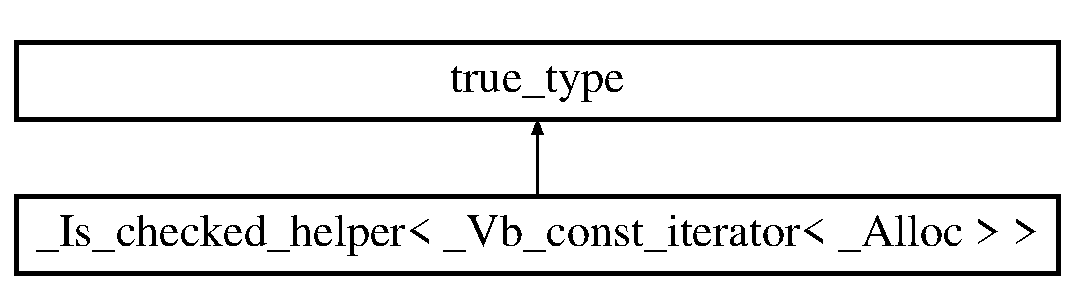
\includegraphics[height=2.000000cm]{struct___is__checked__helper_3_01___vb__const__iterator_3_01___alloc_01_4_01_4}
\end{center}
\end{figure}


\subsection{Detailed Description}
\subsubsection*{template$<$class \+\_\+\+Alloc$>$struct \+\_\+\+Is\+\_\+checked\+\_\+helper$<$ \+\_\+\+Vb\+\_\+const\+\_\+iterator$<$ \+\_\+\+Alloc $>$ $>$}



Definition at line 1886 of file vector.\+h.



The documentation for this struct was generated from the following file\+:\begin{DoxyCompactItemize}
\item 
\hyperlink{vector_8h}{vector.\+h}\end{DoxyCompactItemize}

\hypertarget{struct___is__checked__helper_3_01___vb__iterator_3_01___alloc_01_4_01_4}{\section{\+\_\+\+Is\+\_\+checked\+\_\+helper$<$ \+\_\+\+Vb\+\_\+iterator$<$ \+\_\+\+Alloc $>$ $>$ Struct Template Reference}
\label{struct___is__checked__helper_3_01___vb__iterator_3_01___alloc_01_4_01_4}\index{\+\_\+\+Is\+\_\+checked\+\_\+helper$<$ \+\_\+\+Vb\+\_\+iterator$<$ \+\_\+\+Alloc $>$ $>$@{\+\_\+\+Is\+\_\+checked\+\_\+helper$<$ \+\_\+\+Vb\+\_\+iterator$<$ \+\_\+\+Alloc $>$ $>$}}
}


{\ttfamily \#include $<$vector.\+h$>$}

Inheritance diagram for \+\_\+\+Is\+\_\+checked\+\_\+helper$<$ \+\_\+\+Vb\+\_\+iterator$<$ \+\_\+\+Alloc $>$ $>$\+:\begin{figure}[H]
\begin{center}
\leavevmode
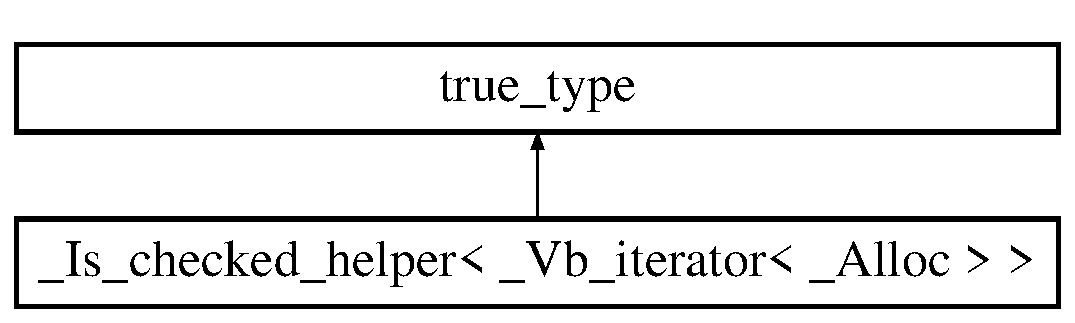
\includegraphics[height=2.000000cm]{struct___is__checked__helper_3_01___vb__iterator_3_01___alloc_01_4_01_4}
\end{center}
\end{figure}


\subsection{Detailed Description}
\subsubsection*{template$<$class \+\_\+\+Alloc$>$struct \+\_\+\+Is\+\_\+checked\+\_\+helper$<$ \+\_\+\+Vb\+\_\+iterator$<$ \+\_\+\+Alloc $>$ $>$}



Definition at line 1992 of file vector.\+h.



The documentation for this struct was generated from the following file\+:\begin{DoxyCompactItemize}
\item 
\hyperlink{vector_8h}{vector.\+h}\end{DoxyCompactItemize}

\hypertarget{class___vb__const__iterator}{\section{\+\_\+\+Vb\+\_\+const\+\_\+iterator$<$ \+\_\+\+Alloc $>$ Class Template Reference}
\label{class___vb__const__iterator}\index{\+\_\+\+Vb\+\_\+const\+\_\+iterator$<$ \+\_\+\+Alloc $>$@{\+\_\+\+Vb\+\_\+const\+\_\+iterator$<$ \+\_\+\+Alloc $>$}}
}


{\ttfamily \#include $<$vector.\+h$>$}

Inheritance diagram for \+\_\+\+Vb\+\_\+const\+\_\+iterator$<$ \+\_\+\+Alloc $>$\+:\begin{figure}[H]
\begin{center}
\leavevmode
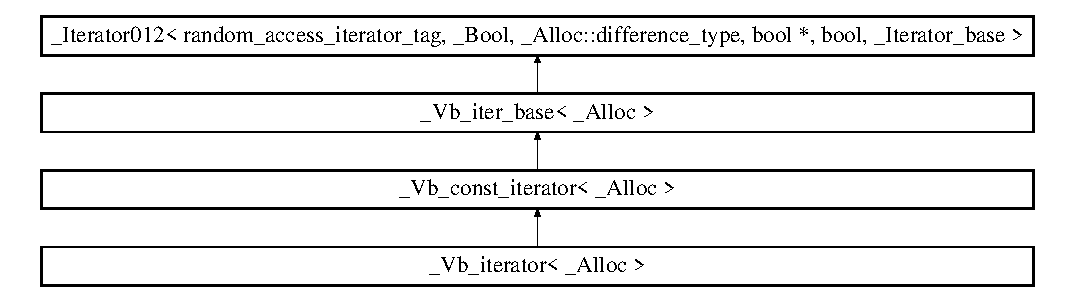
\includegraphics[height=3.607085cm]{class___vb__const__iterator}
\end{center}
\end{figure}
\subsection*{Public Types}
\begin{DoxyCompactItemize}
\item 
typedef \hyperlink{class___vb__iter__base}{\+\_\+\+Vb\+\_\+iter\+\_\+base}$<$ \+\_\+\+Alloc $>$ \hyperlink{class___vb__const__iterator_af4d51819174094e3576a3b45a3e3702f}{\+\_\+\+Mybase}
\item 
typedef \hyperlink{class___vb__const__iterator}{\+\_\+\+Vb\+\_\+const\+\_\+iterator}\\*
$<$ \+\_\+\+Alloc $>$ \hyperlink{class___vb__const__iterator_acab47f643a88497fc0bb9c74afc59fde}{\+\_\+\+Mytype}
\item 
typedef \hyperlink{class___vb__reference}{\+\_\+\+Vb\+\_\+reference}$<$ \+\_\+\+Alloc $>$ \hyperlink{class___vb__const__iterator_a9955dddb0c1346eacd54df1c2cc6e628}{\+\_\+\+Reft}
\item 
typedef bool \hyperlink{class___vb__const__iterator_a7115c71f1b57c74be5291ce71b94b101}{const\+\_\+reference}
\item 
typedef random\+\_\+access\+\_\+iterator\+\_\+tag \hyperlink{class___vb__const__iterator_aa81c954de1d156ee1cc846296d52d38a}{iterator\+\_\+category}
\item 
typedef \+\_\+\+Bool \hyperlink{class___vb__const__iterator_a8b63263ffd9490c057e4c63ae5e4a586}{value\+\_\+type}
\item 
typedef \+\_\+\+Alloc\+::size\+\_\+type \hyperlink{class___vb__const__iterator_ab4d2e8e7d079361dd5e50ac335420b09}{size\+\_\+type}
\item 
typedef \+\_\+\+Alloc\+::difference\+\_\+type \hyperlink{class___vb__const__iterator_a5966ee8cd6e57759253addfa4821de91}{difference\+\_\+type}
\item 
typedef \hyperlink{class___vb__const__iterator_a7115c71f1b57c74be5291ce71b94b101}{const\+\_\+reference} $\ast$ \hyperlink{class___vb__const__iterator_a2da9762fd4a47847dc3901d172b86263}{pointer}
\item 
typedef \hyperlink{class___vb__const__iterator_a7115c71f1b57c74be5291ce71b94b101}{const\+\_\+reference} \hyperlink{class___vb__const__iterator_a15c6fa96bc01a672faec26fbaa7279f4}{reference}
\end{DoxyCompactItemize}
\subsection*{Public Member Functions}
\begin{DoxyCompactItemize}
\item 
\hyperlink{class___vb__const__iterator_adb285202be4920471e0ee9621c2fb31f}{\+\_\+\+Vb\+\_\+const\+\_\+iterator} ()
\item 
\hyperlink{class___vb__const__iterator_a0aa36f9fb0c9ed18175744370fdf4f42}{\+\_\+\+Vb\+\_\+const\+\_\+iterator} (const \hyperlink{vector_8h_a1555a2f621ba9ade75bb9ce8bca77144}{\+\_\+\+Vbase} $\ast$\+\_\+\+Ptr, const \+\_\+\+Container\+\_\+base $\ast$\+\_\+\+Mypvbool)
\item 
\hyperlink{class___vb__const__iterator_a7115c71f1b57c74be5291ce71b94b101}{const\+\_\+reference} \hyperlink{class___vb__const__iterator_aed5662d460401be6fcae3b5a50695e4c}{operator$\ast$} () const 
\item 
\hyperlink{class___vb__const__iterator_acab47f643a88497fc0bb9c74afc59fde}{\+\_\+\+Mytype} \& \hyperlink{class___vb__const__iterator_a7a85954cff3e2e8db90398ffac4dee9b}{operator++} ()
\item 
\hyperlink{class___vb__const__iterator_acab47f643a88497fc0bb9c74afc59fde}{\+\_\+\+Mytype} \hyperlink{class___vb__const__iterator_abac73057e3eb687e73b4b25d2732cf8a}{operator++} (int)
\item 
\hyperlink{class___vb__const__iterator_acab47f643a88497fc0bb9c74afc59fde}{\+\_\+\+Mytype} \& \hyperlink{class___vb__const__iterator_a87d219cd9f573a1dc899a7653232aa4a}{operator-\/-\/} ()
\item 
\hyperlink{class___vb__const__iterator_acab47f643a88497fc0bb9c74afc59fde}{\+\_\+\+Mytype} \hyperlink{class___vb__const__iterator_af75c7595c4e4823e1200ddddf7b46c33}{operator-\/-\/} (int)
\item 
\hyperlink{class___vb__const__iterator_acab47f643a88497fc0bb9c74afc59fde}{\+\_\+\+Mytype} \& \hyperlink{class___vb__const__iterator_adbd033cd0097cc9506216b21e42c82e1}{operator+=} (\hyperlink{class___vb__const__iterator_a5966ee8cd6e57759253addfa4821de91}{difference\+\_\+type} \+\_\+\+Off)
\item 
\hyperlink{class___vb__const__iterator_acab47f643a88497fc0bb9c74afc59fde}{\+\_\+\+Mytype} \hyperlink{class___vb__const__iterator_adf5c43eda935b3b93d09ece16403e054}{operator+} (\hyperlink{class___vb__const__iterator_a5966ee8cd6e57759253addfa4821de91}{difference\+\_\+type} \+\_\+\+Off) const 
\item 
\hyperlink{class___vb__const__iterator_acab47f643a88497fc0bb9c74afc59fde}{\+\_\+\+Mytype} \& \hyperlink{class___vb__const__iterator_a47ea89edd6b70e4b9fa844ca970a1b1c}{operator-\/=} (\hyperlink{class___vb__const__iterator_a5966ee8cd6e57759253addfa4821de91}{difference\+\_\+type} \+\_\+\+Off)
\item 
\hyperlink{class___vb__const__iterator_acab47f643a88497fc0bb9c74afc59fde}{\+\_\+\+Mytype} \hyperlink{class___vb__const__iterator_abc69c09bc5c50a009b88a176254e4569}{operator-\/} (\hyperlink{class___vb__const__iterator_a5966ee8cd6e57759253addfa4821de91}{difference\+\_\+type} \+\_\+\+Off) const 
\item 
\hyperlink{class___vb__const__iterator_a5966ee8cd6e57759253addfa4821de91}{difference\+\_\+type} \hyperlink{class___vb__const__iterator_aff97243bc74d1768dc04576e78f8d31a}{operator-\/} (const \hyperlink{class___vb__const__iterator_acab47f643a88497fc0bb9c74afc59fde}{\+\_\+\+Mytype} \&\+\_\+\+Right) const 
\item 
\hyperlink{class___vb__const__iterator_a7115c71f1b57c74be5291ce71b94b101}{const\+\_\+reference} \hyperlink{class___vb__const__iterator_a64804d7b664d0ee6cbff3a732a72fd8f}{operator\mbox{[}$\,$\mbox{]}} (\hyperlink{class___vb__const__iterator_a5966ee8cd6e57759253addfa4821de91}{difference\+\_\+type} \+\_\+\+Off) const 
\item 
bool \hyperlink{class___vb__const__iterator_a5152323e1194fef039beec538f08f26c}{operator==} (const \hyperlink{class___vb__const__iterator_acab47f643a88497fc0bb9c74afc59fde}{\+\_\+\+Mytype} \&\+\_\+\+Right) const 
\item 
bool \hyperlink{class___vb__const__iterator_abb42b9934c7a8e3709c62561646d555c}{operator!=} (const \hyperlink{class___vb__const__iterator_acab47f643a88497fc0bb9c74afc59fde}{\+\_\+\+Mytype} \&\+\_\+\+Right) const 
\item 
bool \hyperlink{class___vb__const__iterator_ae54ae7c029a964b4ce3ef78d85bc0678}{operator$<$} (const \hyperlink{class___vb__const__iterator_acab47f643a88497fc0bb9c74afc59fde}{\+\_\+\+Mytype} \&\+\_\+\+Right) const 
\item 
bool \hyperlink{class___vb__const__iterator_ab221146db0e163a10e7ff2ed3ba51f73}{operator$>$} (const \hyperlink{class___vb__const__iterator_acab47f643a88497fc0bb9c74afc59fde}{\+\_\+\+Mytype} \&\+\_\+\+Right) const 
\item 
bool \hyperlink{class___vb__const__iterator_ac0ec40c64ced4610694b8a18d8145f03}{operator$<$=} (const \hyperlink{class___vb__const__iterator_acab47f643a88497fc0bb9c74afc59fde}{\+\_\+\+Mytype} \&\+\_\+\+Right) const 
\item 
bool \hyperlink{class___vb__const__iterator_a19ded2784961c7d4600ea4e3181d3c5b}{operator$>$=} (const \hyperlink{class___vb__const__iterator_acab47f643a88497fc0bb9c74afc59fde}{\+\_\+\+Mytype} \&\+\_\+\+Right) const 
\item 
void \hyperlink{class___vb__const__iterator_af359318c3d113596df73f79719f71eee}{\+\_\+\+Compat} (const \hyperlink{class___vb__const__iterator_acab47f643a88497fc0bb9c74afc59fde}{\+\_\+\+Mytype} \&) const 
\item 
void \hyperlink{class___vb__const__iterator_ac429fd3f4687d20a9271e07d61a2504b}{\+\_\+\+Dec} ()
\item 
void \hyperlink{class___vb__const__iterator_a848814eb433056ebf21e58c35c247c1a}{\+\_\+\+Inc} ()
\end{DoxyCompactItemize}
\subsection*{Additional Inherited Members}


\subsection{Detailed Description}
\subsubsection*{template$<$class \+\_\+\+Alloc$>$class \+\_\+\+Vb\+\_\+const\+\_\+iterator$<$ \+\_\+\+Alloc $>$}



Definition at line 1669 of file vector.\+h.



\subsection{Member Typedef Documentation}
\hypertarget{class___vb__const__iterator_af4d51819174094e3576a3b45a3e3702f}{\index{\+\_\+\+Vb\+\_\+const\+\_\+iterator@{\+\_\+\+Vb\+\_\+const\+\_\+iterator}!\+\_\+\+Mybase@{\+\_\+\+Mybase}}
\index{\+\_\+\+Mybase@{\+\_\+\+Mybase}!\+\_\+\+Vb\+\_\+const\+\_\+iterator@{\+\_\+\+Vb\+\_\+const\+\_\+iterator}}
\subsubsection[{\+\_\+\+Mybase}]{\setlength{\rightskip}{0pt plus 5cm}template$<$class \+\_\+\+Alloc$>$ typedef {\bf \+\_\+\+Vb\+\_\+iter\+\_\+base}$<$\+\_\+\+Alloc$>$ {\bf \+\_\+\+Vb\+\_\+const\+\_\+iterator}$<$ \+\_\+\+Alloc $>$\+::{\bf \+\_\+\+Mybase}}}\label{class___vb__const__iterator_af4d51819174094e3576a3b45a3e3702f}


Definition at line 1673 of file vector.\+h.

\hypertarget{class___vb__const__iterator_acab47f643a88497fc0bb9c74afc59fde}{\index{\+\_\+\+Vb\+\_\+const\+\_\+iterator@{\+\_\+\+Vb\+\_\+const\+\_\+iterator}!\+\_\+\+Mytype@{\+\_\+\+Mytype}}
\index{\+\_\+\+Mytype@{\+\_\+\+Mytype}!\+\_\+\+Vb\+\_\+const\+\_\+iterator@{\+\_\+\+Vb\+\_\+const\+\_\+iterator}}
\subsubsection[{\+\_\+\+Mytype}]{\setlength{\rightskip}{0pt plus 5cm}template$<$class \+\_\+\+Alloc$>$ typedef {\bf \+\_\+\+Vb\+\_\+const\+\_\+iterator}$<$\+\_\+\+Alloc$>$ {\bf \+\_\+\+Vb\+\_\+const\+\_\+iterator}$<$ \+\_\+\+Alloc $>$\+::{\bf \+\_\+\+Mytype}}}\label{class___vb__const__iterator_acab47f643a88497fc0bb9c74afc59fde}


Definition at line 1674 of file vector.\+h.

\hypertarget{class___vb__const__iterator_a9955dddb0c1346eacd54df1c2cc6e628}{\index{\+\_\+\+Vb\+\_\+const\+\_\+iterator@{\+\_\+\+Vb\+\_\+const\+\_\+iterator}!\+\_\+\+Reft@{\+\_\+\+Reft}}
\index{\+\_\+\+Reft@{\+\_\+\+Reft}!\+\_\+\+Vb\+\_\+const\+\_\+iterator@{\+\_\+\+Vb\+\_\+const\+\_\+iterator}}
\subsubsection[{\+\_\+\+Reft}]{\setlength{\rightskip}{0pt plus 5cm}template$<$class \+\_\+\+Alloc$>$ typedef {\bf \+\_\+\+Vb\+\_\+reference}$<$\+\_\+\+Alloc$>$ {\bf \+\_\+\+Vb\+\_\+const\+\_\+iterator}$<$ \+\_\+\+Alloc $>$\+::{\bf \+\_\+\+Reft}}}\label{class___vb__const__iterator_a9955dddb0c1346eacd54df1c2cc6e628}


Definition at line 1676 of file vector.\+h.

\hypertarget{class___vb__const__iterator_a7115c71f1b57c74be5291ce71b94b101}{\index{\+\_\+\+Vb\+\_\+const\+\_\+iterator@{\+\_\+\+Vb\+\_\+const\+\_\+iterator}!const\+\_\+reference@{const\+\_\+reference}}
\index{const\+\_\+reference@{const\+\_\+reference}!\+\_\+\+Vb\+\_\+const\+\_\+iterator@{\+\_\+\+Vb\+\_\+const\+\_\+iterator}}
\subsubsection[{const\+\_\+reference}]{\setlength{\rightskip}{0pt plus 5cm}template$<$class \+\_\+\+Alloc$>$ typedef bool {\bf \+\_\+\+Vb\+\_\+const\+\_\+iterator}$<$ \+\_\+\+Alloc $>$\+::{\bf const\+\_\+reference}}}\label{class___vb__const__iterator_a7115c71f1b57c74be5291ce71b94b101}


Definition at line 1677 of file vector.\+h.

\hypertarget{class___vb__const__iterator_a5966ee8cd6e57759253addfa4821de91}{\index{\+\_\+\+Vb\+\_\+const\+\_\+iterator@{\+\_\+\+Vb\+\_\+const\+\_\+iterator}!difference\+\_\+type@{difference\+\_\+type}}
\index{difference\+\_\+type@{difference\+\_\+type}!\+\_\+\+Vb\+\_\+const\+\_\+iterator@{\+\_\+\+Vb\+\_\+const\+\_\+iterator}}
\subsubsection[{difference\+\_\+type}]{\setlength{\rightskip}{0pt plus 5cm}template$<$class \+\_\+\+Alloc$>$ typedef \+\_\+\+Alloc\+::difference\+\_\+type {\bf \+\_\+\+Vb\+\_\+const\+\_\+iterator}$<$ \+\_\+\+Alloc $>$\+::{\bf difference\+\_\+type}}}\label{class___vb__const__iterator_a5966ee8cd6e57759253addfa4821de91}


Definition at line 1682 of file vector.\+h.

\hypertarget{class___vb__const__iterator_aa81c954de1d156ee1cc846296d52d38a}{\index{\+\_\+\+Vb\+\_\+const\+\_\+iterator@{\+\_\+\+Vb\+\_\+const\+\_\+iterator}!iterator\+\_\+category@{iterator\+\_\+category}}
\index{iterator\+\_\+category@{iterator\+\_\+category}!\+\_\+\+Vb\+\_\+const\+\_\+iterator@{\+\_\+\+Vb\+\_\+const\+\_\+iterator}}
\subsubsection[{iterator\+\_\+category}]{\setlength{\rightskip}{0pt plus 5cm}template$<$class \+\_\+\+Alloc$>$ typedef random\+\_\+access\+\_\+iterator\+\_\+tag {\bf \+\_\+\+Vb\+\_\+const\+\_\+iterator}$<$ \+\_\+\+Alloc $>$\+::{\bf iterator\+\_\+category}}}\label{class___vb__const__iterator_aa81c954de1d156ee1cc846296d52d38a}


Definition at line 1679 of file vector.\+h.

\hypertarget{class___vb__const__iterator_a2da9762fd4a47847dc3901d172b86263}{\index{\+\_\+\+Vb\+\_\+const\+\_\+iterator@{\+\_\+\+Vb\+\_\+const\+\_\+iterator}!pointer@{pointer}}
\index{pointer@{pointer}!\+\_\+\+Vb\+\_\+const\+\_\+iterator@{\+\_\+\+Vb\+\_\+const\+\_\+iterator}}
\subsubsection[{pointer}]{\setlength{\rightskip}{0pt plus 5cm}template$<$class \+\_\+\+Alloc$>$ typedef {\bf const\+\_\+reference}$\ast$ {\bf \+\_\+\+Vb\+\_\+const\+\_\+iterator}$<$ \+\_\+\+Alloc $>$\+::{\bf pointer}}}\label{class___vb__const__iterator_a2da9762fd4a47847dc3901d172b86263}


Definition at line 1683 of file vector.\+h.

\hypertarget{class___vb__const__iterator_a15c6fa96bc01a672faec26fbaa7279f4}{\index{\+\_\+\+Vb\+\_\+const\+\_\+iterator@{\+\_\+\+Vb\+\_\+const\+\_\+iterator}!reference@{reference}}
\index{reference@{reference}!\+\_\+\+Vb\+\_\+const\+\_\+iterator@{\+\_\+\+Vb\+\_\+const\+\_\+iterator}}
\subsubsection[{reference}]{\setlength{\rightskip}{0pt plus 5cm}template$<$class \+\_\+\+Alloc$>$ typedef {\bf const\+\_\+reference} {\bf \+\_\+\+Vb\+\_\+const\+\_\+iterator}$<$ \+\_\+\+Alloc $>$\+::{\bf reference}}}\label{class___vb__const__iterator_a15c6fa96bc01a672faec26fbaa7279f4}


Definition at line 1684 of file vector.\+h.

\hypertarget{class___vb__const__iterator_ab4d2e8e7d079361dd5e50ac335420b09}{\index{\+\_\+\+Vb\+\_\+const\+\_\+iterator@{\+\_\+\+Vb\+\_\+const\+\_\+iterator}!size\+\_\+type@{size\+\_\+type}}
\index{size\+\_\+type@{size\+\_\+type}!\+\_\+\+Vb\+\_\+const\+\_\+iterator@{\+\_\+\+Vb\+\_\+const\+\_\+iterator}}
\subsubsection[{size\+\_\+type}]{\setlength{\rightskip}{0pt plus 5cm}template$<$class \+\_\+\+Alloc$>$ typedef \+\_\+\+Alloc\+::size\+\_\+type {\bf \+\_\+\+Vb\+\_\+const\+\_\+iterator}$<$ \+\_\+\+Alloc $>$\+::{\bf size\+\_\+type}}}\label{class___vb__const__iterator_ab4d2e8e7d079361dd5e50ac335420b09}


Definition at line 1681 of file vector.\+h.

\hypertarget{class___vb__const__iterator_a8b63263ffd9490c057e4c63ae5e4a586}{\index{\+\_\+\+Vb\+\_\+const\+\_\+iterator@{\+\_\+\+Vb\+\_\+const\+\_\+iterator}!value\+\_\+type@{value\+\_\+type}}
\index{value\+\_\+type@{value\+\_\+type}!\+\_\+\+Vb\+\_\+const\+\_\+iterator@{\+\_\+\+Vb\+\_\+const\+\_\+iterator}}
\subsubsection[{value\+\_\+type}]{\setlength{\rightskip}{0pt plus 5cm}template$<$class \+\_\+\+Alloc$>$ typedef \+\_\+\+Bool {\bf \+\_\+\+Vb\+\_\+const\+\_\+iterator}$<$ \+\_\+\+Alloc $>$\+::{\bf value\+\_\+type}}}\label{class___vb__const__iterator_a8b63263ffd9490c057e4c63ae5e4a586}


Definition at line 1680 of file vector.\+h.



\subsection{Constructor \& Destructor Documentation}
\hypertarget{class___vb__const__iterator_adb285202be4920471e0ee9621c2fb31f}{\index{\+\_\+\+Vb\+\_\+const\+\_\+iterator@{\+\_\+\+Vb\+\_\+const\+\_\+iterator}!\+\_\+\+Vb\+\_\+const\+\_\+iterator@{\+\_\+\+Vb\+\_\+const\+\_\+iterator}}
\index{\+\_\+\+Vb\+\_\+const\+\_\+iterator@{\+\_\+\+Vb\+\_\+const\+\_\+iterator}!\+\_\+\+Vb\+\_\+const\+\_\+iterator@{\+\_\+\+Vb\+\_\+const\+\_\+iterator}}
\subsubsection[{\+\_\+\+Vb\+\_\+const\+\_\+iterator}]{\setlength{\rightskip}{0pt plus 5cm}template$<$class \+\_\+\+Alloc$>$ {\bf \+\_\+\+Vb\+\_\+const\+\_\+iterator}$<$ \+\_\+\+Alloc $>$\+::{\bf \+\_\+\+Vb\+\_\+const\+\_\+iterator} (
\begin{DoxyParamCaption}
{}
\end{DoxyParamCaption}
)\hspace{0.3cm}{\ttfamily [inline]}}}\label{class___vb__const__iterator_adb285202be4920471e0ee9621c2fb31f}


Definition at line 1686 of file vector.\+h.

\hypertarget{class___vb__const__iterator_a0aa36f9fb0c9ed18175744370fdf4f42}{\index{\+\_\+\+Vb\+\_\+const\+\_\+iterator@{\+\_\+\+Vb\+\_\+const\+\_\+iterator}!\+\_\+\+Vb\+\_\+const\+\_\+iterator@{\+\_\+\+Vb\+\_\+const\+\_\+iterator}}
\index{\+\_\+\+Vb\+\_\+const\+\_\+iterator@{\+\_\+\+Vb\+\_\+const\+\_\+iterator}!\+\_\+\+Vb\+\_\+const\+\_\+iterator@{\+\_\+\+Vb\+\_\+const\+\_\+iterator}}
\subsubsection[{\+\_\+\+Vb\+\_\+const\+\_\+iterator}]{\setlength{\rightskip}{0pt plus 5cm}template$<$class \+\_\+\+Alloc$>$ {\bf \+\_\+\+Vb\+\_\+const\+\_\+iterator}$<$ \+\_\+\+Alloc $>$\+::{\bf \+\_\+\+Vb\+\_\+const\+\_\+iterator} (
\begin{DoxyParamCaption}
\item[{const {\bf \+\_\+\+Vbase} $\ast$}]{\+\_\+\+Ptr, }
\item[{const \+\_\+\+Container\+\_\+base $\ast$}]{\+\_\+\+Mypvbool}
\end{DoxyParamCaption}
)\hspace{0.3cm}{\ttfamily [inline]}}}\label{class___vb__const__iterator_a0aa36f9fb0c9ed18175744370fdf4f42}


Definition at line 1690 of file vector.\+h.



\subsection{Member Function Documentation}
\hypertarget{class___vb__const__iterator_af359318c3d113596df73f79719f71eee}{\index{\+\_\+\+Vb\+\_\+const\+\_\+iterator@{\+\_\+\+Vb\+\_\+const\+\_\+iterator}!\+\_\+\+Compat@{\+\_\+\+Compat}}
\index{\+\_\+\+Compat@{\+\_\+\+Compat}!\+\_\+\+Vb\+\_\+const\+\_\+iterator@{\+\_\+\+Vb\+\_\+const\+\_\+iterator}}
\subsubsection[{\+\_\+\+Compat}]{\setlength{\rightskip}{0pt plus 5cm}template$<$class \+\_\+\+Alloc$>$ void {\bf \+\_\+\+Vb\+\_\+const\+\_\+iterator}$<$ \+\_\+\+Alloc $>$\+::\+\_\+\+Compat (
\begin{DoxyParamCaption}
\item[{const {\bf \+\_\+\+Mytype} \&}]{}
\end{DoxyParamCaption}
) const\hspace{0.3cm}{\ttfamily [inline]}}}\label{class___vb__const__iterator_af359318c3d113596df73f79719f71eee}


Definition at line 1825 of file vector.\+h.

\hypertarget{class___vb__const__iterator_ac429fd3f4687d20a9271e07d61a2504b}{\index{\+\_\+\+Vb\+\_\+const\+\_\+iterator@{\+\_\+\+Vb\+\_\+const\+\_\+iterator}!\+\_\+\+Dec@{\+\_\+\+Dec}}
\index{\+\_\+\+Dec@{\+\_\+\+Dec}!\+\_\+\+Vb\+\_\+const\+\_\+iterator@{\+\_\+\+Vb\+\_\+const\+\_\+iterator}}
\subsubsection[{\+\_\+\+Dec}]{\setlength{\rightskip}{0pt plus 5cm}template$<$class \+\_\+\+Alloc$>$ void {\bf \+\_\+\+Vb\+\_\+const\+\_\+iterator}$<$ \+\_\+\+Alloc $>$\+::\+\_\+\+Dec (
\begin{DoxyParamCaption}
{}
\end{DoxyParamCaption}
)\hspace{0.3cm}{\ttfamily [inline]}}}\label{class___vb__const__iterator_ac429fd3f4687d20a9271e07d61a2504b}


Definition at line 1830 of file vector.\+h.

\hypertarget{class___vb__const__iterator_a848814eb433056ebf21e58c35c247c1a}{\index{\+\_\+\+Vb\+\_\+const\+\_\+iterator@{\+\_\+\+Vb\+\_\+const\+\_\+iterator}!\+\_\+\+Inc@{\+\_\+\+Inc}}
\index{\+\_\+\+Inc@{\+\_\+\+Inc}!\+\_\+\+Vb\+\_\+const\+\_\+iterator@{\+\_\+\+Vb\+\_\+const\+\_\+iterator}}
\subsubsection[{\+\_\+\+Inc}]{\setlength{\rightskip}{0pt plus 5cm}template$<$class \+\_\+\+Alloc$>$ void {\bf \+\_\+\+Vb\+\_\+const\+\_\+iterator}$<$ \+\_\+\+Alloc $>$\+::\+\_\+\+Inc (
\begin{DoxyParamCaption}
{}
\end{DoxyParamCaption}
)\hspace{0.3cm}{\ttfamily [inline]}}}\label{class___vb__const__iterator_a848814eb433056ebf21e58c35c247c1a}


Definition at line 1853 of file vector.\+h.

\hypertarget{class___vb__const__iterator_abb42b9934c7a8e3709c62561646d555c}{\index{\+\_\+\+Vb\+\_\+const\+\_\+iterator@{\+\_\+\+Vb\+\_\+const\+\_\+iterator}!operator"!=@{operator"!=}}
\index{operator"!=@{operator"!=}!\+\_\+\+Vb\+\_\+const\+\_\+iterator@{\+\_\+\+Vb\+\_\+const\+\_\+iterator}}
\subsubsection[{operator"!=}]{\setlength{\rightskip}{0pt plus 5cm}template$<$class \+\_\+\+Alloc$>$ bool {\bf \+\_\+\+Vb\+\_\+const\+\_\+iterator}$<$ \+\_\+\+Alloc $>$\+::operator!= (
\begin{DoxyParamCaption}
\item[{const {\bf \+\_\+\+Mytype} \&}]{\+\_\+\+Right}
\end{DoxyParamCaption}
) const\hspace{0.3cm}{\ttfamily [inline]}}}\label{class___vb__const__iterator_abb42b9934c7a8e3709c62561646d555c}


Definition at line 1781 of file vector.\+h.

\hypertarget{class___vb__const__iterator_aed5662d460401be6fcae3b5a50695e4c}{\index{\+\_\+\+Vb\+\_\+const\+\_\+iterator@{\+\_\+\+Vb\+\_\+const\+\_\+iterator}!operator$\ast$@{operator$\ast$}}
\index{operator$\ast$@{operator$\ast$}!\+\_\+\+Vb\+\_\+const\+\_\+iterator@{\+\_\+\+Vb\+\_\+const\+\_\+iterator}}
\subsubsection[{operator$\ast$}]{\setlength{\rightskip}{0pt plus 5cm}template$<$class \+\_\+\+Alloc$>$ {\bf const\+\_\+reference} {\bf \+\_\+\+Vb\+\_\+const\+\_\+iterator}$<$ \+\_\+\+Alloc $>$\+::operator$\ast$ (
\begin{DoxyParamCaption}
{}
\end{DoxyParamCaption}
) const\hspace{0.3cm}{\ttfamily [inline]}}}\label{class___vb__const__iterator_aed5662d460401be6fcae3b5a50695e4c}


Definition at line 1695 of file vector.\+h.

\hypertarget{class___vb__const__iterator_adf5c43eda935b3b93d09ece16403e054}{\index{\+\_\+\+Vb\+\_\+const\+\_\+iterator@{\+\_\+\+Vb\+\_\+const\+\_\+iterator}!operator+@{operator+}}
\index{operator+@{operator+}!\+\_\+\+Vb\+\_\+const\+\_\+iterator@{\+\_\+\+Vb\+\_\+const\+\_\+iterator}}
\subsubsection[{operator+}]{\setlength{\rightskip}{0pt plus 5cm}template$<$class \+\_\+\+Alloc$>$ {\bf \+\_\+\+Mytype} {\bf \+\_\+\+Vb\+\_\+const\+\_\+iterator}$<$ \+\_\+\+Alloc $>$\+::operator+ (
\begin{DoxyParamCaption}
\item[{{\bf difference\+\_\+type}}]{\+\_\+\+Off}
\end{DoxyParamCaption}
) const\hspace{0.3cm}{\ttfamily [inline]}}}\label{class___vb__const__iterator_adf5c43eda935b3b93d09ece16403e054}


Definition at line 1743 of file vector.\+h.

\hypertarget{class___vb__const__iterator_a7a85954cff3e2e8db90398ffac4dee9b}{\index{\+\_\+\+Vb\+\_\+const\+\_\+iterator@{\+\_\+\+Vb\+\_\+const\+\_\+iterator}!operator++@{operator++}}
\index{operator++@{operator++}!\+\_\+\+Vb\+\_\+const\+\_\+iterator@{\+\_\+\+Vb\+\_\+const\+\_\+iterator}}
\subsubsection[{operator++}]{\setlength{\rightskip}{0pt plus 5cm}template$<$class \+\_\+\+Alloc$>$ {\bf \+\_\+\+Mytype}\& {\bf \+\_\+\+Vb\+\_\+const\+\_\+iterator}$<$ \+\_\+\+Alloc $>$\+::operator++ (
\begin{DoxyParamCaption}
{}
\end{DoxyParamCaption}
)\hspace{0.3cm}{\ttfamily [inline]}}}\label{class___vb__const__iterator_a7a85954cff3e2e8db90398ffac4dee9b}


Definition at line 1700 of file vector.\+h.

\hypertarget{class___vb__const__iterator_abac73057e3eb687e73b4b25d2732cf8a}{\index{\+\_\+\+Vb\+\_\+const\+\_\+iterator@{\+\_\+\+Vb\+\_\+const\+\_\+iterator}!operator++@{operator++}}
\index{operator++@{operator++}!\+\_\+\+Vb\+\_\+const\+\_\+iterator@{\+\_\+\+Vb\+\_\+const\+\_\+iterator}}
\subsubsection[{operator++}]{\setlength{\rightskip}{0pt plus 5cm}template$<$class \+\_\+\+Alloc$>$ {\bf \+\_\+\+Mytype} {\bf \+\_\+\+Vb\+\_\+const\+\_\+iterator}$<$ \+\_\+\+Alloc $>$\+::operator++ (
\begin{DoxyParamCaption}
\item[{int}]{}
\end{DoxyParamCaption}
)\hspace{0.3cm}{\ttfamily [inline]}}}\label{class___vb__const__iterator_abac73057e3eb687e73b4b25d2732cf8a}


Definition at line 1706 of file vector.\+h.

\hypertarget{class___vb__const__iterator_adbd033cd0097cc9506216b21e42c82e1}{\index{\+\_\+\+Vb\+\_\+const\+\_\+iterator@{\+\_\+\+Vb\+\_\+const\+\_\+iterator}!operator+=@{operator+=}}
\index{operator+=@{operator+=}!\+\_\+\+Vb\+\_\+const\+\_\+iterator@{\+\_\+\+Vb\+\_\+const\+\_\+iterator}}
\subsubsection[{operator+=}]{\setlength{\rightskip}{0pt plus 5cm}template$<$class \+\_\+\+Alloc$>$ {\bf \+\_\+\+Mytype}\& {\bf \+\_\+\+Vb\+\_\+const\+\_\+iterator}$<$ \+\_\+\+Alloc $>$\+::operator+= (
\begin{DoxyParamCaption}
\item[{{\bf difference\+\_\+type}}]{\+\_\+\+Off}
\end{DoxyParamCaption}
)\hspace{0.3cm}{\ttfamily [inline]}}}\label{class___vb__const__iterator_adbd033cd0097cc9506216b21e42c82e1}


Definition at line 1726 of file vector.\+h.

\hypertarget{class___vb__const__iterator_abc69c09bc5c50a009b88a176254e4569}{\index{\+\_\+\+Vb\+\_\+const\+\_\+iterator@{\+\_\+\+Vb\+\_\+const\+\_\+iterator}!operator-\/@{operator-\/}}
\index{operator-\/@{operator-\/}!\+\_\+\+Vb\+\_\+const\+\_\+iterator@{\+\_\+\+Vb\+\_\+const\+\_\+iterator}}
\subsubsection[{operator-\/}]{\setlength{\rightskip}{0pt plus 5cm}template$<$class \+\_\+\+Alloc$>$ {\bf \+\_\+\+Mytype} {\bf \+\_\+\+Vb\+\_\+const\+\_\+iterator}$<$ \+\_\+\+Alloc $>$\+::operator-\/ (
\begin{DoxyParamCaption}
\item[{{\bf difference\+\_\+type}}]{\+\_\+\+Off}
\end{DoxyParamCaption}
) const\hspace{0.3cm}{\ttfamily [inline]}}}\label{class___vb__const__iterator_abc69c09bc5c50a009b88a176254e4569}


Definition at line 1754 of file vector.\+h.

\hypertarget{class___vb__const__iterator_aff97243bc74d1768dc04576e78f8d31a}{\index{\+\_\+\+Vb\+\_\+const\+\_\+iterator@{\+\_\+\+Vb\+\_\+const\+\_\+iterator}!operator-\/@{operator-\/}}
\index{operator-\/@{operator-\/}!\+\_\+\+Vb\+\_\+const\+\_\+iterator@{\+\_\+\+Vb\+\_\+const\+\_\+iterator}}
\subsubsection[{operator-\/}]{\setlength{\rightskip}{0pt plus 5cm}template$<$class \+\_\+\+Alloc$>$ {\bf difference\+\_\+type} {\bf \+\_\+\+Vb\+\_\+const\+\_\+iterator}$<$ \+\_\+\+Alloc $>$\+::operator-\/ (
\begin{DoxyParamCaption}
\item[{const {\bf \+\_\+\+Mytype} \&}]{\+\_\+\+Right}
\end{DoxyParamCaption}
) const\hspace{0.3cm}{\ttfamily [inline]}}}\label{class___vb__const__iterator_aff97243bc74d1768dc04576e78f8d31a}


Definition at line 1760 of file vector.\+h.

\hypertarget{class___vb__const__iterator_a87d219cd9f573a1dc899a7653232aa4a}{\index{\+\_\+\+Vb\+\_\+const\+\_\+iterator@{\+\_\+\+Vb\+\_\+const\+\_\+iterator}!operator-\/-\/@{operator-\/-\/}}
\index{operator-\/-\/@{operator-\/-\/}!\+\_\+\+Vb\+\_\+const\+\_\+iterator@{\+\_\+\+Vb\+\_\+const\+\_\+iterator}}
\subsubsection[{operator-\/-\/}]{\setlength{\rightskip}{0pt plus 5cm}template$<$class \+\_\+\+Alloc$>$ {\bf \+\_\+\+Mytype}\& {\bf \+\_\+\+Vb\+\_\+const\+\_\+iterator}$<$ \+\_\+\+Alloc $>$\+::operator-\/-\/ (
\begin{DoxyParamCaption}
{}
\end{DoxyParamCaption}
)\hspace{0.3cm}{\ttfamily [inline]}}}\label{class___vb__const__iterator_a87d219cd9f573a1dc899a7653232aa4a}


Definition at line 1713 of file vector.\+h.

\hypertarget{class___vb__const__iterator_af75c7595c4e4823e1200ddddf7b46c33}{\index{\+\_\+\+Vb\+\_\+const\+\_\+iterator@{\+\_\+\+Vb\+\_\+const\+\_\+iterator}!operator-\/-\/@{operator-\/-\/}}
\index{operator-\/-\/@{operator-\/-\/}!\+\_\+\+Vb\+\_\+const\+\_\+iterator@{\+\_\+\+Vb\+\_\+const\+\_\+iterator}}
\subsubsection[{operator-\/-\/}]{\setlength{\rightskip}{0pt plus 5cm}template$<$class \+\_\+\+Alloc$>$ {\bf \+\_\+\+Mytype} {\bf \+\_\+\+Vb\+\_\+const\+\_\+iterator}$<$ \+\_\+\+Alloc $>$\+::operator-\/-\/ (
\begin{DoxyParamCaption}
\item[{int}]{}
\end{DoxyParamCaption}
)\hspace{0.3cm}{\ttfamily [inline]}}}\label{class___vb__const__iterator_af75c7595c4e4823e1200ddddf7b46c33}


Definition at line 1719 of file vector.\+h.

\hypertarget{class___vb__const__iterator_a47ea89edd6b70e4b9fa844ca970a1b1c}{\index{\+\_\+\+Vb\+\_\+const\+\_\+iterator@{\+\_\+\+Vb\+\_\+const\+\_\+iterator}!operator-\/=@{operator-\/=}}
\index{operator-\/=@{operator-\/=}!\+\_\+\+Vb\+\_\+const\+\_\+iterator@{\+\_\+\+Vb\+\_\+const\+\_\+iterator}}
\subsubsection[{operator-\/=}]{\setlength{\rightskip}{0pt plus 5cm}template$<$class \+\_\+\+Alloc$>$ {\bf \+\_\+\+Mytype}\& {\bf \+\_\+\+Vb\+\_\+const\+\_\+iterator}$<$ \+\_\+\+Alloc $>$\+::operator-\/= (
\begin{DoxyParamCaption}
\item[{{\bf difference\+\_\+type}}]{\+\_\+\+Off}
\end{DoxyParamCaption}
)\hspace{0.3cm}{\ttfamily [inline]}}}\label{class___vb__const__iterator_a47ea89edd6b70e4b9fa844ca970a1b1c}


Definition at line 1749 of file vector.\+h.

\hypertarget{class___vb__const__iterator_ae54ae7c029a964b4ce3ef78d85bc0678}{\index{\+\_\+\+Vb\+\_\+const\+\_\+iterator@{\+\_\+\+Vb\+\_\+const\+\_\+iterator}!operator$<$@{operator$<$}}
\index{operator$<$@{operator$<$}!\+\_\+\+Vb\+\_\+const\+\_\+iterator@{\+\_\+\+Vb\+\_\+const\+\_\+iterator}}
\subsubsection[{operator$<$}]{\setlength{\rightskip}{0pt plus 5cm}template$<$class \+\_\+\+Alloc$>$ bool {\bf \+\_\+\+Vb\+\_\+const\+\_\+iterator}$<$ \+\_\+\+Alloc $>$\+::operator$<$ (
\begin{DoxyParamCaption}
\item[{const {\bf \+\_\+\+Mytype} \&}]{\+\_\+\+Right}
\end{DoxyParamCaption}
) const\hspace{0.3cm}{\ttfamily [inline]}}}\label{class___vb__const__iterator_ae54ae7c029a964b4ce3ef78d85bc0678}


Definition at line 1786 of file vector.\+h.

\hypertarget{class___vb__const__iterator_ac0ec40c64ced4610694b8a18d8145f03}{\index{\+\_\+\+Vb\+\_\+const\+\_\+iterator@{\+\_\+\+Vb\+\_\+const\+\_\+iterator}!operator$<$=@{operator$<$=}}
\index{operator$<$=@{operator$<$=}!\+\_\+\+Vb\+\_\+const\+\_\+iterator@{\+\_\+\+Vb\+\_\+const\+\_\+iterator}}
\subsubsection[{operator$<$=}]{\setlength{\rightskip}{0pt plus 5cm}template$<$class \+\_\+\+Alloc$>$ bool {\bf \+\_\+\+Vb\+\_\+const\+\_\+iterator}$<$ \+\_\+\+Alloc $>$\+::operator$<$= (
\begin{DoxyParamCaption}
\item[{const {\bf \+\_\+\+Mytype} \&}]{\+\_\+\+Right}
\end{DoxyParamCaption}
) const\hspace{0.3cm}{\ttfamily [inline]}}}\label{class___vb__const__iterator_ac0ec40c64ced4610694b8a18d8145f03}


Definition at line 1799 of file vector.\+h.

\hypertarget{class___vb__const__iterator_a5152323e1194fef039beec538f08f26c}{\index{\+\_\+\+Vb\+\_\+const\+\_\+iterator@{\+\_\+\+Vb\+\_\+const\+\_\+iterator}!operator==@{operator==}}
\index{operator==@{operator==}!\+\_\+\+Vb\+\_\+const\+\_\+iterator@{\+\_\+\+Vb\+\_\+const\+\_\+iterator}}
\subsubsection[{operator==}]{\setlength{\rightskip}{0pt plus 5cm}template$<$class \+\_\+\+Alloc$>$ bool {\bf \+\_\+\+Vb\+\_\+const\+\_\+iterator}$<$ \+\_\+\+Alloc $>$\+::operator== (
\begin{DoxyParamCaption}
\item[{const {\bf \+\_\+\+Mytype} \&}]{\+\_\+\+Right}
\end{DoxyParamCaption}
) const\hspace{0.3cm}{\ttfamily [inline]}}}\label{class___vb__const__iterator_a5152323e1194fef039beec538f08f26c}


Definition at line 1774 of file vector.\+h.

\hypertarget{class___vb__const__iterator_ab221146db0e163a10e7ff2ed3ba51f73}{\index{\+\_\+\+Vb\+\_\+const\+\_\+iterator@{\+\_\+\+Vb\+\_\+const\+\_\+iterator}!operator$>$@{operator$>$}}
\index{operator$>$@{operator$>$}!\+\_\+\+Vb\+\_\+const\+\_\+iterator@{\+\_\+\+Vb\+\_\+const\+\_\+iterator}}
\subsubsection[{operator$>$}]{\setlength{\rightskip}{0pt plus 5cm}template$<$class \+\_\+\+Alloc$>$ bool {\bf \+\_\+\+Vb\+\_\+const\+\_\+iterator}$<$ \+\_\+\+Alloc $>$\+::operator$>$ (
\begin{DoxyParamCaption}
\item[{const {\bf \+\_\+\+Mytype} \&}]{\+\_\+\+Right}
\end{DoxyParamCaption}
) const\hspace{0.3cm}{\ttfamily [inline]}}}\label{class___vb__const__iterator_ab221146db0e163a10e7ff2ed3ba51f73}


Definition at line 1794 of file vector.\+h.

\hypertarget{class___vb__const__iterator_a19ded2784961c7d4600ea4e3181d3c5b}{\index{\+\_\+\+Vb\+\_\+const\+\_\+iterator@{\+\_\+\+Vb\+\_\+const\+\_\+iterator}!operator$>$=@{operator$>$=}}
\index{operator$>$=@{operator$>$=}!\+\_\+\+Vb\+\_\+const\+\_\+iterator@{\+\_\+\+Vb\+\_\+const\+\_\+iterator}}
\subsubsection[{operator$>$=}]{\setlength{\rightskip}{0pt plus 5cm}template$<$class \+\_\+\+Alloc$>$ bool {\bf \+\_\+\+Vb\+\_\+const\+\_\+iterator}$<$ \+\_\+\+Alloc $>$\+::operator$>$= (
\begin{DoxyParamCaption}
\item[{const {\bf \+\_\+\+Mytype} \&}]{\+\_\+\+Right}
\end{DoxyParamCaption}
) const\hspace{0.3cm}{\ttfamily [inline]}}}\label{class___vb__const__iterator_a19ded2784961c7d4600ea4e3181d3c5b}


Definition at line 1804 of file vector.\+h.

\hypertarget{class___vb__const__iterator_a64804d7b664d0ee6cbff3a732a72fd8f}{\index{\+\_\+\+Vb\+\_\+const\+\_\+iterator@{\+\_\+\+Vb\+\_\+const\+\_\+iterator}!operator\mbox{[}$\,$\mbox{]}@{operator[]}}
\index{operator\mbox{[}$\,$\mbox{]}@{operator[]}!\+\_\+\+Vb\+\_\+const\+\_\+iterator@{\+\_\+\+Vb\+\_\+const\+\_\+iterator}}
\subsubsection[{operator[]}]{\setlength{\rightskip}{0pt plus 5cm}template$<$class \+\_\+\+Alloc$>$ {\bf const\+\_\+reference} {\bf \+\_\+\+Vb\+\_\+const\+\_\+iterator}$<$ \+\_\+\+Alloc $>$\+::operator\mbox{[}$\,$\mbox{]} (
\begin{DoxyParamCaption}
\item[{{\bf difference\+\_\+type}}]{\+\_\+\+Off}
\end{DoxyParamCaption}
) const\hspace{0.3cm}{\ttfamily [inline]}}}\label{class___vb__const__iterator_a64804d7b664d0ee6cbff3a732a72fd8f}


Definition at line 1769 of file vector.\+h.



The documentation for this class was generated from the following file\+:\begin{DoxyCompactItemize}
\item 
\hyperlink{vector_8h}{vector.\+h}\end{DoxyCompactItemize}

\hypertarget{class___vb__iter__base}{\section{\+\_\+\+Vb\+\_\+iter\+\_\+base$<$ \+\_\+\+Alloc $>$ Class Template Reference}
\label{class___vb__iter__base}\index{\+\_\+\+Vb\+\_\+iter\+\_\+base$<$ \+\_\+\+Alloc $>$@{\+\_\+\+Vb\+\_\+iter\+\_\+base$<$ \+\_\+\+Alloc $>$}}
}


{\ttfamily \#include $<$vector.\+h$>$}

Inheritance diagram for \+\_\+\+Vb\+\_\+iter\+\_\+base$<$ \+\_\+\+Alloc $>$\+:\begin{figure}[H]
\begin{center}
\leavevmode
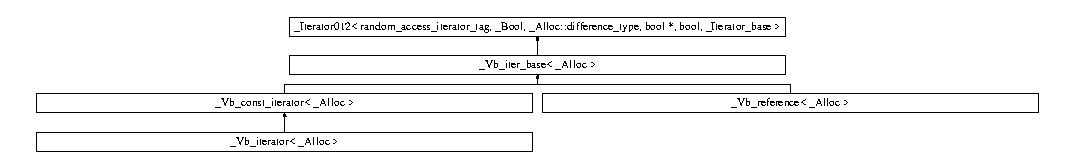
\includegraphics[height=1.803543cm]{class___vb__iter__base}
\end{center}
\end{figure}
\subsection*{Public Types}
\begin{DoxyCompactItemize}
\item 
typedef \+\_\+\+Alloc\+::size\+\_\+type \hyperlink{class___vb__iter__base_a43b848fb198e38fc0e831a270c07a60d}{\+\_\+\+Sizet}
\item 
typedef \hyperlink{classvector}{vector}$<$ \+\_\+\+Bool, \+\_\+\+Alloc $>$ \hyperlink{class___vb__iter__base_af0f146606d0f7f220d58bfa7ffada3b7}{\+\_\+\+Mycont}
\end{DoxyCompactItemize}
\subsection*{Public Member Functions}
\begin{DoxyCompactItemize}
\item 
\hyperlink{class___vb__iter__base_ae4cbe1ace2e26c6fcf673a15cf881d82}{\+\_\+\+Vb\+\_\+iter\+\_\+base} ()
\item 
\hyperlink{class___vb__iter__base_a7847ca8c4f1c49cc78f3ef0a5be406d4}{\+\_\+\+Vb\+\_\+iter\+\_\+base} (const \hyperlink{vector_8h_a1555a2f621ba9ade75bb9ce8bca77144}{\+\_\+\+Vbase} $\ast$\+\_\+\+Ptr, \hyperlink{class___vb__iter__base_a43b848fb198e38fc0e831a270c07a60d}{\+\_\+\+Sizet} \+\_\+\+Off, const \+\_\+\+Container\+\_\+base $\ast$\+\_\+\+Mypvbool)
\item 
int \hyperlink{class___vb__iter__base_a916ac903fceeced2345bdd305ec66fbc}{\+\_\+\+Valid} (\hyperlink{class___vb__iter__base_a43b848fb198e38fc0e831a270c07a60d}{\+\_\+\+Sizet} \+\_\+\+Inc) const 
\end{DoxyCompactItemize}
\subsection*{Public Attributes}
\begin{DoxyCompactItemize}
\item 
const \hyperlink{vector_8h_a1555a2f621ba9ade75bb9ce8bca77144}{\+\_\+\+Vbase} $\ast$ \hyperlink{class___vb__iter__base_a5b1b58fc2e3a55121f0c227c8077fb05}{\+\_\+\+Myptr}
\item 
\hyperlink{class___vb__iter__base_a43b848fb198e38fc0e831a270c07a60d}{\+\_\+\+Sizet} \hyperlink{class___vb__iter__base_a83e2c6bfcf7b8ba34cf6b80997a24b25}{\+\_\+\+Myoff}
\end{DoxyCompactItemize}


\subsection{Detailed Description}
\subsubsection*{template$<$class \+\_\+\+Alloc$>$class \+\_\+\+Vb\+\_\+iter\+\_\+base$<$ \+\_\+\+Alloc $>$}



Definition at line 1541 of file vector.\+h.



\subsection{Member Typedef Documentation}
\hypertarget{class___vb__iter__base_af0f146606d0f7f220d58bfa7ffada3b7}{\index{\+\_\+\+Vb\+\_\+iter\+\_\+base@{\+\_\+\+Vb\+\_\+iter\+\_\+base}!\+\_\+\+Mycont@{\+\_\+\+Mycont}}
\index{\+\_\+\+Mycont@{\+\_\+\+Mycont}!\+\_\+\+Vb\+\_\+iter\+\_\+base@{\+\_\+\+Vb\+\_\+iter\+\_\+base}}
\subsubsection[{\+\_\+\+Mycont}]{\setlength{\rightskip}{0pt plus 5cm}template$<$class \+\_\+\+Alloc $>$ typedef {\bf vector}$<$\+\_\+\+Bool, \+\_\+\+Alloc$>$ {\bf \+\_\+\+Vb\+\_\+iter\+\_\+base}$<$ \+\_\+\+Alloc $>$\+::{\bf \+\_\+\+Mycont}}}\label{class___vb__iter__base_af0f146606d0f7f220d58bfa7ffada3b7}


Definition at line 1551 of file vector.\+h.

\hypertarget{class___vb__iter__base_a43b848fb198e38fc0e831a270c07a60d}{\index{\+\_\+\+Vb\+\_\+iter\+\_\+base@{\+\_\+\+Vb\+\_\+iter\+\_\+base}!\+\_\+\+Sizet@{\+\_\+\+Sizet}}
\index{\+\_\+\+Sizet@{\+\_\+\+Sizet}!\+\_\+\+Vb\+\_\+iter\+\_\+base@{\+\_\+\+Vb\+\_\+iter\+\_\+base}}
\subsubsection[{\+\_\+\+Sizet}]{\setlength{\rightskip}{0pt plus 5cm}template$<$class \+\_\+\+Alloc $>$ typedef \+\_\+\+Alloc\+::size\+\_\+type {\bf \+\_\+\+Vb\+\_\+iter\+\_\+base}$<$ \+\_\+\+Alloc $>$\+::{\bf \+\_\+\+Sizet}}}\label{class___vb__iter__base_a43b848fb198e38fc0e831a270c07a60d}


Definition at line 1550 of file vector.\+h.



\subsection{Constructor \& Destructor Documentation}
\hypertarget{class___vb__iter__base_ae4cbe1ace2e26c6fcf673a15cf881d82}{\index{\+\_\+\+Vb\+\_\+iter\+\_\+base@{\+\_\+\+Vb\+\_\+iter\+\_\+base}!\+\_\+\+Vb\+\_\+iter\+\_\+base@{\+\_\+\+Vb\+\_\+iter\+\_\+base}}
\index{\+\_\+\+Vb\+\_\+iter\+\_\+base@{\+\_\+\+Vb\+\_\+iter\+\_\+base}!\+\_\+\+Vb\+\_\+iter\+\_\+base@{\+\_\+\+Vb\+\_\+iter\+\_\+base}}
\subsubsection[{\+\_\+\+Vb\+\_\+iter\+\_\+base}]{\setlength{\rightskip}{0pt plus 5cm}template$<$class \+\_\+\+Alloc $>$ {\bf \+\_\+\+Vb\+\_\+iter\+\_\+base}$<$ \+\_\+\+Alloc $>$\+::{\bf \+\_\+\+Vb\+\_\+iter\+\_\+base} (
\begin{DoxyParamCaption}
{}
\end{DoxyParamCaption}
)\hspace{0.3cm}{\ttfamily [inline]}}}\label{class___vb__iter__base_ae4cbe1ace2e26c6fcf673a15cf881d82}


Definition at line 1553 of file vector.\+h.

\hypertarget{class___vb__iter__base_a7847ca8c4f1c49cc78f3ef0a5be406d4}{\index{\+\_\+\+Vb\+\_\+iter\+\_\+base@{\+\_\+\+Vb\+\_\+iter\+\_\+base}!\+\_\+\+Vb\+\_\+iter\+\_\+base@{\+\_\+\+Vb\+\_\+iter\+\_\+base}}
\index{\+\_\+\+Vb\+\_\+iter\+\_\+base@{\+\_\+\+Vb\+\_\+iter\+\_\+base}!\+\_\+\+Vb\+\_\+iter\+\_\+base@{\+\_\+\+Vb\+\_\+iter\+\_\+base}}
\subsubsection[{\+\_\+\+Vb\+\_\+iter\+\_\+base}]{\setlength{\rightskip}{0pt plus 5cm}template$<$class \+\_\+\+Alloc $>$ {\bf \+\_\+\+Vb\+\_\+iter\+\_\+base}$<$ \+\_\+\+Alloc $>$\+::{\bf \+\_\+\+Vb\+\_\+iter\+\_\+base} (
\begin{DoxyParamCaption}
\item[{const {\bf \+\_\+\+Vbase} $\ast$}]{\+\_\+\+Ptr, }
\item[{{\bf \+\_\+\+Sizet}}]{\+\_\+\+Off, }
\item[{const \+\_\+\+Container\+\_\+base $\ast$}]{\+\_\+\+Mypvbool}
\end{DoxyParamCaption}
)\hspace{0.3cm}{\ttfamily [inline]}}}\label{class___vb__iter__base_a7847ca8c4f1c49cc78f3ef0a5be406d4}


Definition at line 1558 of file vector.\+h.



\subsection{Member Function Documentation}
\hypertarget{class___vb__iter__base_a916ac903fceeced2345bdd305ec66fbc}{\index{\+\_\+\+Vb\+\_\+iter\+\_\+base@{\+\_\+\+Vb\+\_\+iter\+\_\+base}!\+\_\+\+Valid@{\+\_\+\+Valid}}
\index{\+\_\+\+Valid@{\+\_\+\+Valid}!\+\_\+\+Vb\+\_\+iter\+\_\+base@{\+\_\+\+Vb\+\_\+iter\+\_\+base}}
\subsubsection[{\+\_\+\+Valid}]{\setlength{\rightskip}{0pt plus 5cm}template$<$class \+\_\+\+Alloc $>$ int {\bf \+\_\+\+Vb\+\_\+iter\+\_\+base}$<$ \+\_\+\+Alloc $>$\+::\+\_\+\+Valid (
\begin{DoxyParamCaption}
\item[{{\bf \+\_\+\+Sizet}}]{\+\_\+\+Inc}
\end{DoxyParamCaption}
) const\hspace{0.3cm}{\ttfamily [inline]}}}\label{class___vb__iter__base_a916ac903fceeced2345bdd305ec66fbc}


Definition at line 1565 of file vector.\+h.



\subsection{Member Data Documentation}
\hypertarget{class___vb__iter__base_a83e2c6bfcf7b8ba34cf6b80997a24b25}{\index{\+\_\+\+Vb\+\_\+iter\+\_\+base@{\+\_\+\+Vb\+\_\+iter\+\_\+base}!\+\_\+\+Myoff@{\+\_\+\+Myoff}}
\index{\+\_\+\+Myoff@{\+\_\+\+Myoff}!\+\_\+\+Vb\+\_\+iter\+\_\+base@{\+\_\+\+Vb\+\_\+iter\+\_\+base}}
\subsubsection[{\+\_\+\+Myoff}]{\setlength{\rightskip}{0pt plus 5cm}template$<$class \+\_\+\+Alloc $>$ {\bf \+\_\+\+Sizet} {\bf \+\_\+\+Vb\+\_\+iter\+\_\+base}$<$ \+\_\+\+Alloc $>$\+::\+\_\+\+Myoff}}\label{class___vb__iter__base_a83e2c6bfcf7b8ba34cf6b80997a24b25}


Definition at line 1582 of file vector.\+h.

\hypertarget{class___vb__iter__base_a5b1b58fc2e3a55121f0c227c8077fb05}{\index{\+\_\+\+Vb\+\_\+iter\+\_\+base@{\+\_\+\+Vb\+\_\+iter\+\_\+base}!\+\_\+\+Myptr@{\+\_\+\+Myptr}}
\index{\+\_\+\+Myptr@{\+\_\+\+Myptr}!\+\_\+\+Vb\+\_\+iter\+\_\+base@{\+\_\+\+Vb\+\_\+iter\+\_\+base}}
\subsubsection[{\+\_\+\+Myptr}]{\setlength{\rightskip}{0pt plus 5cm}template$<$class \+\_\+\+Alloc $>$ const {\bf \+\_\+\+Vbase}$\ast$ {\bf \+\_\+\+Vb\+\_\+iter\+\_\+base}$<$ \+\_\+\+Alloc $>$\+::\+\_\+\+Myptr}}\label{class___vb__iter__base_a5b1b58fc2e3a55121f0c227c8077fb05}


Definition at line 1581 of file vector.\+h.



The documentation for this class was generated from the following file\+:\begin{DoxyCompactItemize}
\item 
\hyperlink{vector_8h}{vector.\+h}\end{DoxyCompactItemize}

\hypertarget{class___vb__iterator}{\section{\+\_\+\+Vb\+\_\+iterator$<$ \+\_\+\+Alloc $>$ Class Template Reference}
\label{class___vb__iterator}\index{\+\_\+\+Vb\+\_\+iterator$<$ \+\_\+\+Alloc $>$@{\+\_\+\+Vb\+\_\+iterator$<$ \+\_\+\+Alloc $>$}}
}


{\ttfamily \#include $<$vector.\+h$>$}

Inheritance diagram for \+\_\+\+Vb\+\_\+iterator$<$ \+\_\+\+Alloc $>$\+:\begin{figure}[H]
\begin{center}
\leavevmode
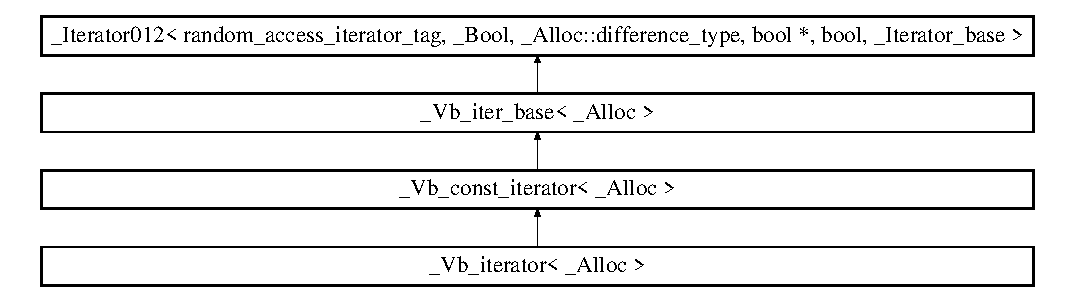
\includegraphics[height=3.607085cm]{class___vb__iterator}
\end{center}
\end{figure}
\subsection*{Public Types}
\begin{DoxyCompactItemize}
\item 
typedef \hyperlink{class___vb__const__iterator}{\+\_\+\+Vb\+\_\+const\+\_\+iterator}\\*
$<$ \+\_\+\+Alloc $>$ \hyperlink{class___vb__iterator_ad51a01f62e10e7da8f8aa6393e5fa4db}{\+\_\+\+Mybase}
\item 
typedef \hyperlink{class___vb__iterator}{\+\_\+\+Vb\+\_\+iterator}$<$ \+\_\+\+Alloc $>$ \hyperlink{class___vb__iterator_a2fff8ac5ba795d77033915aa2a358403}{\+\_\+\+Mytype}
\item 
typedef \hyperlink{class___vb__reference}{\+\_\+\+Vb\+\_\+reference}$<$ \+\_\+\+Alloc $>$ \hyperlink{class___vb__iterator_a30e2e5d349b96c5988cd782e69c58161}{\+\_\+\+Reft}
\item 
typedef bool \hyperlink{class___vb__iterator_ad346337dd66c8689d4017f3b74b7d50f}{const\+\_\+reference}
\item 
typedef random\+\_\+access\+\_\+iterator\+\_\+tag \hyperlink{class___vb__iterator_a637be1a0886bd658f935ce022e5bfe09}{iterator\+\_\+category}
\item 
typedef \+\_\+\+Bool \hyperlink{class___vb__iterator_ae9282be9870338a878afd631ba072555}{value\+\_\+type}
\item 
typedef \+\_\+\+Alloc\+::size\+\_\+type \hyperlink{class___vb__iterator_a9dfed016c4d7f08f4bac304af81f8397}{size\+\_\+type}
\item 
typedef \+\_\+\+Alloc\+::difference\+\_\+type \hyperlink{class___vb__iterator_a148abf77b7a6501dc20581b9f4b1dfe4}{difference\+\_\+type}
\item 
typedef \hyperlink{class___vb__const__iterator_a9955dddb0c1346eacd54df1c2cc6e628}{\+\_\+\+Reft} $\ast$ \hyperlink{class___vb__iterator_abfdae002074201202d96a0200ca2ab23}{pointer}
\item 
typedef \hyperlink{class___vb__const__iterator_a9955dddb0c1346eacd54df1c2cc6e628}{\+\_\+\+Reft} \hyperlink{class___vb__iterator_a0fd0a2449dbc621f22117b1999cb1929}{reference}
\end{DoxyCompactItemize}
\subsection*{Public Member Functions}
\begin{DoxyCompactItemize}
\item 
\hyperlink{class___vb__iterator_ac1d30a9ec5f9304ebf9856eea41f8768}{\+\_\+\+Vb\+\_\+iterator} ()
\item 
\hyperlink{class___vb__iterator_a259ac0c62c3d2ade3e451b622d9937c6}{\+\_\+\+Vb\+\_\+iterator} (\hyperlink{vector_8h_a1555a2f621ba9ade75bb9ce8bca77144}{\+\_\+\+Vbase} $\ast$\+\_\+\+Ptr, \+\_\+\+Container\+\_\+base $\ast$\+\_\+\+Mypvbool)
\item 
\hyperlink{class___vb__const__iterator_a15c6fa96bc01a672faec26fbaa7279f4}{reference} \hyperlink{class___vb__iterator_a44aebc25b6cfc48f07c432152dbeaeff}{operator$\ast$} () const 
\item 
\hyperlink{class___vb__const__iterator_acab47f643a88497fc0bb9c74afc59fde}{\+\_\+\+Mytype} \& \hyperlink{class___vb__iterator_aee7ea7599386765c1ee06623816e6552}{operator++} ()
\item 
\hyperlink{class___vb__const__iterator_acab47f643a88497fc0bb9c74afc59fde}{\+\_\+\+Mytype} \hyperlink{class___vb__iterator_a318d5bc0c8b61bcacf0005e274abf42e}{operator++} (int)
\item 
\hyperlink{class___vb__const__iterator_acab47f643a88497fc0bb9c74afc59fde}{\+\_\+\+Mytype} \& \hyperlink{class___vb__iterator_aab9b62a59fab1ef0454913af894e221e}{operator-\/-\/} ()
\item 
\hyperlink{class___vb__const__iterator_acab47f643a88497fc0bb9c74afc59fde}{\+\_\+\+Mytype} \hyperlink{class___vb__iterator_a174b7ac71912c9ac58f7616483133fd0}{operator-\/-\/} (int)
\item 
\hyperlink{class___vb__const__iterator_acab47f643a88497fc0bb9c74afc59fde}{\+\_\+\+Mytype} \& \hyperlink{class___vb__iterator_aaf8d830a65c1968c3086d8fbca761655}{operator+=} (\hyperlink{class___vb__const__iterator_a5966ee8cd6e57759253addfa4821de91}{difference\+\_\+type} \+\_\+\+Off)
\item 
\hyperlink{class___vb__const__iterator_acab47f643a88497fc0bb9c74afc59fde}{\+\_\+\+Mytype} \hyperlink{class___vb__iterator_ae754ace3f1b47879b156e94330ec720d}{operator+} (\hyperlink{class___vb__const__iterator_a5966ee8cd6e57759253addfa4821de91}{difference\+\_\+type} \+\_\+\+Off) const 
\item 
\hyperlink{class___vb__const__iterator_acab47f643a88497fc0bb9c74afc59fde}{\+\_\+\+Mytype} \& \hyperlink{class___vb__iterator_a526df7970bf944cea861058d24f7ba44}{operator-\/=} (\hyperlink{class___vb__const__iterator_a5966ee8cd6e57759253addfa4821de91}{difference\+\_\+type} \+\_\+\+Off)
\item 
\hyperlink{class___vb__const__iterator_acab47f643a88497fc0bb9c74afc59fde}{\+\_\+\+Mytype} \hyperlink{class___vb__iterator_aee20ce70ac1a5b71170f20e7aa7cb0c7}{operator-\/} (\hyperlink{class___vb__const__iterator_a5966ee8cd6e57759253addfa4821de91}{difference\+\_\+type} \+\_\+\+Off) const 
\item 
\hyperlink{class___vb__const__iterator_a5966ee8cd6e57759253addfa4821de91}{difference\+\_\+type} \hyperlink{class___vb__iterator_a99022c5a1a92e41f4eb02becde1062f0}{operator-\/} (const \hyperlink{class___vb__const__iterator_af4d51819174094e3576a3b45a3e3702f}{\+\_\+\+Mybase} \&\+\_\+\+Right) const 
\item 
\hyperlink{class___vb__const__iterator_a15c6fa96bc01a672faec26fbaa7279f4}{reference} \hyperlink{class___vb__iterator_ae5b762680c39e9fd49faead971121594}{operator\mbox{[}$\,$\mbox{]}} (\hyperlink{class___vb__const__iterator_a5966ee8cd6e57759253addfa4821de91}{difference\+\_\+type} \+\_\+\+Off) const 
\end{DoxyCompactItemize}
\subsection*{Additional Inherited Members}


\subsection{Detailed Description}
\subsubsection*{template$<$class \+\_\+\+Alloc$>$class \+\_\+\+Vb\+\_\+iterator$<$ \+\_\+\+Alloc $>$}



Definition at line 1893 of file vector.\+h.



\subsection{Member Typedef Documentation}
\hypertarget{class___vb__iterator_ad51a01f62e10e7da8f8aa6393e5fa4db}{\index{\+\_\+\+Vb\+\_\+iterator@{\+\_\+\+Vb\+\_\+iterator}!\+\_\+\+Mybase@{\+\_\+\+Mybase}}
\index{\+\_\+\+Mybase@{\+\_\+\+Mybase}!\+\_\+\+Vb\+\_\+iterator@{\+\_\+\+Vb\+\_\+iterator}}
\subsubsection[{\+\_\+\+Mybase}]{\setlength{\rightskip}{0pt plus 5cm}template$<$class \+\_\+\+Alloc$>$ typedef {\bf \+\_\+\+Vb\+\_\+const\+\_\+iterator}$<$\+\_\+\+Alloc$>$ {\bf \+\_\+\+Vb\+\_\+iterator}$<$ \+\_\+\+Alloc $>$\+::{\bf \+\_\+\+Mybase}}}\label{class___vb__iterator_ad51a01f62e10e7da8f8aa6393e5fa4db}


Definition at line 1897 of file vector.\+h.

\hypertarget{class___vb__iterator_a2fff8ac5ba795d77033915aa2a358403}{\index{\+\_\+\+Vb\+\_\+iterator@{\+\_\+\+Vb\+\_\+iterator}!\+\_\+\+Mytype@{\+\_\+\+Mytype}}
\index{\+\_\+\+Mytype@{\+\_\+\+Mytype}!\+\_\+\+Vb\+\_\+iterator@{\+\_\+\+Vb\+\_\+iterator}}
\subsubsection[{\+\_\+\+Mytype}]{\setlength{\rightskip}{0pt plus 5cm}template$<$class \+\_\+\+Alloc$>$ typedef {\bf \+\_\+\+Vb\+\_\+iterator}$<$\+\_\+\+Alloc$>$ {\bf \+\_\+\+Vb\+\_\+iterator}$<$ \+\_\+\+Alloc $>$\+::{\bf \+\_\+\+Mytype}}}\label{class___vb__iterator_a2fff8ac5ba795d77033915aa2a358403}


Definition at line 1898 of file vector.\+h.

\hypertarget{class___vb__iterator_a30e2e5d349b96c5988cd782e69c58161}{\index{\+\_\+\+Vb\+\_\+iterator@{\+\_\+\+Vb\+\_\+iterator}!\+\_\+\+Reft@{\+\_\+\+Reft}}
\index{\+\_\+\+Reft@{\+\_\+\+Reft}!\+\_\+\+Vb\+\_\+iterator@{\+\_\+\+Vb\+\_\+iterator}}
\subsubsection[{\+\_\+\+Reft}]{\setlength{\rightskip}{0pt plus 5cm}template$<$class \+\_\+\+Alloc$>$ typedef {\bf \+\_\+\+Vb\+\_\+reference}$<$\+\_\+\+Alloc$>$ {\bf \+\_\+\+Vb\+\_\+iterator}$<$ \+\_\+\+Alloc $>$\+::{\bf \+\_\+\+Reft}}}\label{class___vb__iterator_a30e2e5d349b96c5988cd782e69c58161}


Definition at line 1900 of file vector.\+h.

\hypertarget{class___vb__iterator_ad346337dd66c8689d4017f3b74b7d50f}{\index{\+\_\+\+Vb\+\_\+iterator@{\+\_\+\+Vb\+\_\+iterator}!const\+\_\+reference@{const\+\_\+reference}}
\index{const\+\_\+reference@{const\+\_\+reference}!\+\_\+\+Vb\+\_\+iterator@{\+\_\+\+Vb\+\_\+iterator}}
\subsubsection[{const\+\_\+reference}]{\setlength{\rightskip}{0pt plus 5cm}template$<$class \+\_\+\+Alloc$>$ typedef bool {\bf \+\_\+\+Vb\+\_\+iterator}$<$ \+\_\+\+Alloc $>$\+::{\bf const\+\_\+reference}}}\label{class___vb__iterator_ad346337dd66c8689d4017f3b74b7d50f}


Definition at line 1901 of file vector.\+h.

\hypertarget{class___vb__iterator_a148abf77b7a6501dc20581b9f4b1dfe4}{\index{\+\_\+\+Vb\+\_\+iterator@{\+\_\+\+Vb\+\_\+iterator}!difference\+\_\+type@{difference\+\_\+type}}
\index{difference\+\_\+type@{difference\+\_\+type}!\+\_\+\+Vb\+\_\+iterator@{\+\_\+\+Vb\+\_\+iterator}}
\subsubsection[{difference\+\_\+type}]{\setlength{\rightskip}{0pt plus 5cm}template$<$class \+\_\+\+Alloc$>$ typedef \+\_\+\+Alloc\+::difference\+\_\+type {\bf \+\_\+\+Vb\+\_\+iterator}$<$ \+\_\+\+Alloc $>$\+::{\bf difference\+\_\+type}}}\label{class___vb__iterator_a148abf77b7a6501dc20581b9f4b1dfe4}


Definition at line 1906 of file vector.\+h.

\hypertarget{class___vb__iterator_a637be1a0886bd658f935ce022e5bfe09}{\index{\+\_\+\+Vb\+\_\+iterator@{\+\_\+\+Vb\+\_\+iterator}!iterator\+\_\+category@{iterator\+\_\+category}}
\index{iterator\+\_\+category@{iterator\+\_\+category}!\+\_\+\+Vb\+\_\+iterator@{\+\_\+\+Vb\+\_\+iterator}}
\subsubsection[{iterator\+\_\+category}]{\setlength{\rightskip}{0pt plus 5cm}template$<$class \+\_\+\+Alloc$>$ typedef random\+\_\+access\+\_\+iterator\+\_\+tag {\bf \+\_\+\+Vb\+\_\+iterator}$<$ \+\_\+\+Alloc $>$\+::{\bf iterator\+\_\+category}}}\label{class___vb__iterator_a637be1a0886bd658f935ce022e5bfe09}


Definition at line 1903 of file vector.\+h.

\hypertarget{class___vb__iterator_abfdae002074201202d96a0200ca2ab23}{\index{\+\_\+\+Vb\+\_\+iterator@{\+\_\+\+Vb\+\_\+iterator}!pointer@{pointer}}
\index{pointer@{pointer}!\+\_\+\+Vb\+\_\+iterator@{\+\_\+\+Vb\+\_\+iterator}}
\subsubsection[{pointer}]{\setlength{\rightskip}{0pt plus 5cm}template$<$class \+\_\+\+Alloc$>$ typedef {\bf \+\_\+\+Reft}$\ast$ {\bf \+\_\+\+Vb\+\_\+iterator}$<$ \+\_\+\+Alloc $>$\+::{\bf pointer}}}\label{class___vb__iterator_abfdae002074201202d96a0200ca2ab23}


Definition at line 1907 of file vector.\+h.

\hypertarget{class___vb__iterator_a0fd0a2449dbc621f22117b1999cb1929}{\index{\+\_\+\+Vb\+\_\+iterator@{\+\_\+\+Vb\+\_\+iterator}!reference@{reference}}
\index{reference@{reference}!\+\_\+\+Vb\+\_\+iterator@{\+\_\+\+Vb\+\_\+iterator}}
\subsubsection[{reference}]{\setlength{\rightskip}{0pt plus 5cm}template$<$class \+\_\+\+Alloc$>$ typedef {\bf \+\_\+\+Reft} {\bf \+\_\+\+Vb\+\_\+iterator}$<$ \+\_\+\+Alloc $>$\+::{\bf reference}}}\label{class___vb__iterator_a0fd0a2449dbc621f22117b1999cb1929}


Definition at line 1908 of file vector.\+h.

\hypertarget{class___vb__iterator_a9dfed016c4d7f08f4bac304af81f8397}{\index{\+\_\+\+Vb\+\_\+iterator@{\+\_\+\+Vb\+\_\+iterator}!size\+\_\+type@{size\+\_\+type}}
\index{size\+\_\+type@{size\+\_\+type}!\+\_\+\+Vb\+\_\+iterator@{\+\_\+\+Vb\+\_\+iterator}}
\subsubsection[{size\+\_\+type}]{\setlength{\rightskip}{0pt plus 5cm}template$<$class \+\_\+\+Alloc$>$ typedef \+\_\+\+Alloc\+::size\+\_\+type {\bf \+\_\+\+Vb\+\_\+iterator}$<$ \+\_\+\+Alloc $>$\+::{\bf size\+\_\+type}}}\label{class___vb__iterator_a9dfed016c4d7f08f4bac304af81f8397}


Definition at line 1905 of file vector.\+h.

\hypertarget{class___vb__iterator_ae9282be9870338a878afd631ba072555}{\index{\+\_\+\+Vb\+\_\+iterator@{\+\_\+\+Vb\+\_\+iterator}!value\+\_\+type@{value\+\_\+type}}
\index{value\+\_\+type@{value\+\_\+type}!\+\_\+\+Vb\+\_\+iterator@{\+\_\+\+Vb\+\_\+iterator}}
\subsubsection[{value\+\_\+type}]{\setlength{\rightskip}{0pt plus 5cm}template$<$class \+\_\+\+Alloc$>$ typedef \+\_\+\+Bool {\bf \+\_\+\+Vb\+\_\+iterator}$<$ \+\_\+\+Alloc $>$\+::{\bf value\+\_\+type}}}\label{class___vb__iterator_ae9282be9870338a878afd631ba072555}


Definition at line 1904 of file vector.\+h.



\subsection{Constructor \& Destructor Documentation}
\hypertarget{class___vb__iterator_ac1d30a9ec5f9304ebf9856eea41f8768}{\index{\+\_\+\+Vb\+\_\+iterator@{\+\_\+\+Vb\+\_\+iterator}!\+\_\+\+Vb\+\_\+iterator@{\+\_\+\+Vb\+\_\+iterator}}
\index{\+\_\+\+Vb\+\_\+iterator@{\+\_\+\+Vb\+\_\+iterator}!\+\_\+\+Vb\+\_\+iterator@{\+\_\+\+Vb\+\_\+iterator}}
\subsubsection[{\+\_\+\+Vb\+\_\+iterator}]{\setlength{\rightskip}{0pt plus 5cm}template$<$class \+\_\+\+Alloc$>$ {\bf \+\_\+\+Vb\+\_\+iterator}$<$ \+\_\+\+Alloc $>$\+::{\bf \+\_\+\+Vb\+\_\+iterator} (
\begin{DoxyParamCaption}
{}
\end{DoxyParamCaption}
)\hspace{0.3cm}{\ttfamily [inline]}}}\label{class___vb__iterator_ac1d30a9ec5f9304ebf9856eea41f8768}


Definition at line 1910 of file vector.\+h.

\hypertarget{class___vb__iterator_a259ac0c62c3d2ade3e451b622d9937c6}{\index{\+\_\+\+Vb\+\_\+iterator@{\+\_\+\+Vb\+\_\+iterator}!\+\_\+\+Vb\+\_\+iterator@{\+\_\+\+Vb\+\_\+iterator}}
\index{\+\_\+\+Vb\+\_\+iterator@{\+\_\+\+Vb\+\_\+iterator}!\+\_\+\+Vb\+\_\+iterator@{\+\_\+\+Vb\+\_\+iterator}}
\subsubsection[{\+\_\+\+Vb\+\_\+iterator}]{\setlength{\rightskip}{0pt plus 5cm}template$<$class \+\_\+\+Alloc$>$ {\bf \+\_\+\+Vb\+\_\+iterator}$<$ \+\_\+\+Alloc $>$\+::{\bf \+\_\+\+Vb\+\_\+iterator} (
\begin{DoxyParamCaption}
\item[{{\bf \+\_\+\+Vbase} $\ast$}]{\+\_\+\+Ptr, }
\item[{\+\_\+\+Container\+\_\+base $\ast$}]{\+\_\+\+Mypvbool}
\end{DoxyParamCaption}
)\hspace{0.3cm}{\ttfamily [inline]}}}\label{class___vb__iterator_a259ac0c62c3d2ade3e451b622d9937c6}


Definition at line 1914 of file vector.\+h.



\subsection{Member Function Documentation}
\hypertarget{class___vb__iterator_a44aebc25b6cfc48f07c432152dbeaeff}{\index{\+\_\+\+Vb\+\_\+iterator@{\+\_\+\+Vb\+\_\+iterator}!operator$\ast$@{operator$\ast$}}
\index{operator$\ast$@{operator$\ast$}!\+\_\+\+Vb\+\_\+iterator@{\+\_\+\+Vb\+\_\+iterator}}
\subsubsection[{operator$\ast$}]{\setlength{\rightskip}{0pt plus 5cm}template$<$class \+\_\+\+Alloc$>$ {\bf reference} {\bf \+\_\+\+Vb\+\_\+iterator}$<$ \+\_\+\+Alloc $>$\+::operator$\ast$ (
\begin{DoxyParamCaption}
{}
\end{DoxyParamCaption}
) const\hspace{0.3cm}{\ttfamily [inline]}}}\label{class___vb__iterator_a44aebc25b6cfc48f07c432152dbeaeff}


Definition at line 1919 of file vector.\+h.

\hypertarget{class___vb__iterator_ae754ace3f1b47879b156e94330ec720d}{\index{\+\_\+\+Vb\+\_\+iterator@{\+\_\+\+Vb\+\_\+iterator}!operator+@{operator+}}
\index{operator+@{operator+}!\+\_\+\+Vb\+\_\+iterator@{\+\_\+\+Vb\+\_\+iterator}}
\subsubsection[{operator+}]{\setlength{\rightskip}{0pt plus 5cm}template$<$class \+\_\+\+Alloc$>$ {\bf \+\_\+\+Mytype} {\bf \+\_\+\+Vb\+\_\+iterator}$<$ \+\_\+\+Alloc $>$\+::operator+ (
\begin{DoxyParamCaption}
\item[{{\bf difference\+\_\+type}}]{\+\_\+\+Off}
\end{DoxyParamCaption}
) const\hspace{0.3cm}{\ttfamily [inline]}}}\label{class___vb__iterator_ae754ace3f1b47879b156e94330ec720d}


Definition at line 1956 of file vector.\+h.

\hypertarget{class___vb__iterator_aee7ea7599386765c1ee06623816e6552}{\index{\+\_\+\+Vb\+\_\+iterator@{\+\_\+\+Vb\+\_\+iterator}!operator++@{operator++}}
\index{operator++@{operator++}!\+\_\+\+Vb\+\_\+iterator@{\+\_\+\+Vb\+\_\+iterator}}
\subsubsection[{operator++}]{\setlength{\rightskip}{0pt plus 5cm}template$<$class \+\_\+\+Alloc$>$ {\bf \+\_\+\+Mytype}\& {\bf \+\_\+\+Vb\+\_\+iterator}$<$ \+\_\+\+Alloc $>$\+::operator++ (
\begin{DoxyParamCaption}
{}
\end{DoxyParamCaption}
)\hspace{0.3cm}{\ttfamily [inline]}}}\label{class___vb__iterator_aee7ea7599386765c1ee06623816e6552}


Definition at line 1924 of file vector.\+h.

\hypertarget{class___vb__iterator_a318d5bc0c8b61bcacf0005e274abf42e}{\index{\+\_\+\+Vb\+\_\+iterator@{\+\_\+\+Vb\+\_\+iterator}!operator++@{operator++}}
\index{operator++@{operator++}!\+\_\+\+Vb\+\_\+iterator@{\+\_\+\+Vb\+\_\+iterator}}
\subsubsection[{operator++}]{\setlength{\rightskip}{0pt plus 5cm}template$<$class \+\_\+\+Alloc$>$ {\bf \+\_\+\+Mytype} {\bf \+\_\+\+Vb\+\_\+iterator}$<$ \+\_\+\+Alloc $>$\+::operator++ (
\begin{DoxyParamCaption}
\item[{int}]{}
\end{DoxyParamCaption}
)\hspace{0.3cm}{\ttfamily [inline]}}}\label{class___vb__iterator_a318d5bc0c8b61bcacf0005e274abf42e}


Definition at line 1930 of file vector.\+h.

\hypertarget{class___vb__iterator_aaf8d830a65c1968c3086d8fbca761655}{\index{\+\_\+\+Vb\+\_\+iterator@{\+\_\+\+Vb\+\_\+iterator}!operator+=@{operator+=}}
\index{operator+=@{operator+=}!\+\_\+\+Vb\+\_\+iterator@{\+\_\+\+Vb\+\_\+iterator}}
\subsubsection[{operator+=}]{\setlength{\rightskip}{0pt plus 5cm}template$<$class \+\_\+\+Alloc$>$ {\bf \+\_\+\+Mytype}\& {\bf \+\_\+\+Vb\+\_\+iterator}$<$ \+\_\+\+Alloc $>$\+::operator+= (
\begin{DoxyParamCaption}
\item[{{\bf difference\+\_\+type}}]{\+\_\+\+Off}
\end{DoxyParamCaption}
)\hspace{0.3cm}{\ttfamily [inline]}}}\label{class___vb__iterator_aaf8d830a65c1968c3086d8fbca761655}


Definition at line 1950 of file vector.\+h.

\hypertarget{class___vb__iterator_aee20ce70ac1a5b71170f20e7aa7cb0c7}{\index{\+\_\+\+Vb\+\_\+iterator@{\+\_\+\+Vb\+\_\+iterator}!operator-\/@{operator-\/}}
\index{operator-\/@{operator-\/}!\+\_\+\+Vb\+\_\+iterator@{\+\_\+\+Vb\+\_\+iterator}}
\subsubsection[{operator-\/}]{\setlength{\rightskip}{0pt plus 5cm}template$<$class \+\_\+\+Alloc$>$ {\bf \+\_\+\+Mytype} {\bf \+\_\+\+Vb\+\_\+iterator}$<$ \+\_\+\+Alloc $>$\+::operator-\/ (
\begin{DoxyParamCaption}
\item[{{\bf difference\+\_\+type}}]{\+\_\+\+Off}
\end{DoxyParamCaption}
) const\hspace{0.3cm}{\ttfamily [inline]}}}\label{class___vb__iterator_aee20ce70ac1a5b71170f20e7aa7cb0c7}


Definition at line 1967 of file vector.\+h.

\hypertarget{class___vb__iterator_a99022c5a1a92e41f4eb02becde1062f0}{\index{\+\_\+\+Vb\+\_\+iterator@{\+\_\+\+Vb\+\_\+iterator}!operator-\/@{operator-\/}}
\index{operator-\/@{operator-\/}!\+\_\+\+Vb\+\_\+iterator@{\+\_\+\+Vb\+\_\+iterator}}
\subsubsection[{operator-\/}]{\setlength{\rightskip}{0pt plus 5cm}template$<$class \+\_\+\+Alloc$>$ {\bf difference\+\_\+type} {\bf \+\_\+\+Vb\+\_\+iterator}$<$ \+\_\+\+Alloc $>$\+::operator-\/ (
\begin{DoxyParamCaption}
\item[{const {\bf \+\_\+\+Mybase} \&}]{\+\_\+\+Right}
\end{DoxyParamCaption}
) const\hspace{0.3cm}{\ttfamily [inline]}}}\label{class___vb__iterator_a99022c5a1a92e41f4eb02becde1062f0}


Definition at line 1973 of file vector.\+h.

\hypertarget{class___vb__iterator_aab9b62a59fab1ef0454913af894e221e}{\index{\+\_\+\+Vb\+\_\+iterator@{\+\_\+\+Vb\+\_\+iterator}!operator-\/-\/@{operator-\/-\/}}
\index{operator-\/-\/@{operator-\/-\/}!\+\_\+\+Vb\+\_\+iterator@{\+\_\+\+Vb\+\_\+iterator}}
\subsubsection[{operator-\/-\/}]{\setlength{\rightskip}{0pt plus 5cm}template$<$class \+\_\+\+Alloc$>$ {\bf \+\_\+\+Mytype}\& {\bf \+\_\+\+Vb\+\_\+iterator}$<$ \+\_\+\+Alloc $>$\+::operator-\/-\/ (
\begin{DoxyParamCaption}
{}
\end{DoxyParamCaption}
)\hspace{0.3cm}{\ttfamily [inline]}}}\label{class___vb__iterator_aab9b62a59fab1ef0454913af894e221e}


Definition at line 1937 of file vector.\+h.

\hypertarget{class___vb__iterator_a174b7ac71912c9ac58f7616483133fd0}{\index{\+\_\+\+Vb\+\_\+iterator@{\+\_\+\+Vb\+\_\+iterator}!operator-\/-\/@{operator-\/-\/}}
\index{operator-\/-\/@{operator-\/-\/}!\+\_\+\+Vb\+\_\+iterator@{\+\_\+\+Vb\+\_\+iterator}}
\subsubsection[{operator-\/-\/}]{\setlength{\rightskip}{0pt plus 5cm}template$<$class \+\_\+\+Alloc$>$ {\bf \+\_\+\+Mytype} {\bf \+\_\+\+Vb\+\_\+iterator}$<$ \+\_\+\+Alloc $>$\+::operator-\/-\/ (
\begin{DoxyParamCaption}
\item[{int}]{}
\end{DoxyParamCaption}
)\hspace{0.3cm}{\ttfamily [inline]}}}\label{class___vb__iterator_a174b7ac71912c9ac58f7616483133fd0}


Definition at line 1943 of file vector.\+h.

\hypertarget{class___vb__iterator_a526df7970bf944cea861058d24f7ba44}{\index{\+\_\+\+Vb\+\_\+iterator@{\+\_\+\+Vb\+\_\+iterator}!operator-\/=@{operator-\/=}}
\index{operator-\/=@{operator-\/=}!\+\_\+\+Vb\+\_\+iterator@{\+\_\+\+Vb\+\_\+iterator}}
\subsubsection[{operator-\/=}]{\setlength{\rightskip}{0pt plus 5cm}template$<$class \+\_\+\+Alloc$>$ {\bf \+\_\+\+Mytype}\& {\bf \+\_\+\+Vb\+\_\+iterator}$<$ \+\_\+\+Alloc $>$\+::operator-\/= (
\begin{DoxyParamCaption}
\item[{{\bf difference\+\_\+type}}]{\+\_\+\+Off}
\end{DoxyParamCaption}
)\hspace{0.3cm}{\ttfamily [inline]}}}\label{class___vb__iterator_a526df7970bf944cea861058d24f7ba44}


Definition at line 1962 of file vector.\+h.

\hypertarget{class___vb__iterator_ae5b762680c39e9fd49faead971121594}{\index{\+\_\+\+Vb\+\_\+iterator@{\+\_\+\+Vb\+\_\+iterator}!operator\mbox{[}$\,$\mbox{]}@{operator[]}}
\index{operator\mbox{[}$\,$\mbox{]}@{operator[]}!\+\_\+\+Vb\+\_\+iterator@{\+\_\+\+Vb\+\_\+iterator}}
\subsubsection[{operator[]}]{\setlength{\rightskip}{0pt plus 5cm}template$<$class \+\_\+\+Alloc$>$ {\bf reference} {\bf \+\_\+\+Vb\+\_\+iterator}$<$ \+\_\+\+Alloc $>$\+::operator\mbox{[}$\,$\mbox{]} (
\begin{DoxyParamCaption}
\item[{{\bf difference\+\_\+type}}]{\+\_\+\+Off}
\end{DoxyParamCaption}
) const\hspace{0.3cm}{\ttfamily [inline]}}}\label{class___vb__iterator_ae5b762680c39e9fd49faead971121594}


Definition at line 1978 of file vector.\+h.



The documentation for this class was generated from the following file\+:\begin{DoxyCompactItemize}
\item 
\hyperlink{vector_8h}{vector.\+h}\end{DoxyCompactItemize}

\hypertarget{class___vb__reference}{\section{\+\_\+\+Vb\+\_\+reference$<$ \+\_\+\+Alloc $>$ Class Template Reference}
\label{class___vb__reference}\index{\+\_\+\+Vb\+\_\+reference$<$ \+\_\+\+Alloc $>$@{\+\_\+\+Vb\+\_\+reference$<$ \+\_\+\+Alloc $>$}}
}


{\ttfamily \#include $<$vector.\+h$>$}

Inheritance diagram for \+\_\+\+Vb\+\_\+reference$<$ \+\_\+\+Alloc $>$\+:\begin{figure}[H]
\begin{center}
\leavevmode
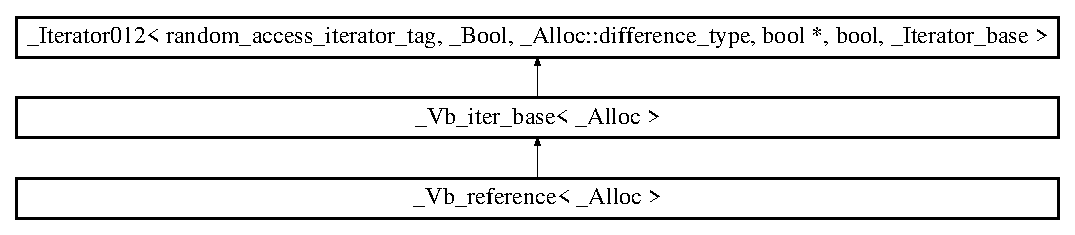
\includegraphics[height=2.705314cm]{class___vb__reference}
\end{center}
\end{figure}
\subsection*{Public Types}
\begin{DoxyCompactItemize}
\item 
typedef \hyperlink{class___vb__iter__base}{\+\_\+\+Vb\+\_\+iter\+\_\+base}$<$ \+\_\+\+Alloc $>$ \hyperlink{class___vb__reference_a9885641a0d5bfa12196f9b2fa497fd0d}{\+\_\+\+Mybase}
\item 
typedef \hyperlink{class___vb__reference}{\+\_\+\+Vb\+\_\+reference}$<$ \+\_\+\+Alloc $>$ \hyperlink{class___vb__reference_aa1f6faf9ee4e99f42b9ba34d0ca98705}{\+\_\+\+Mytype}
\end{DoxyCompactItemize}
\subsection*{Public Member Functions}
\begin{DoxyCompactItemize}
\item 
\hyperlink{class___vb__reference_aa4a4484ac726d499dd0fa063a7dfa2fa}{\+\_\+\+Vb\+\_\+reference} ()
\item 
\hyperlink{class___vb__reference_ad8ef4be97d965a69ed7d3985316e99f8}{\+\_\+\+Vb\+\_\+reference} (const \hyperlink{class___vb__reference_a9885641a0d5bfa12196f9b2fa497fd0d}{\+\_\+\+Mybase} \&\+\_\+\+Right)
\item 
\hyperlink{class___vb__reference_aa1f6faf9ee4e99f42b9ba34d0ca98705}{\+\_\+\+Mytype} \& \hyperlink{class___vb__reference_ab22320956a99cb27af2facc712d66421}{operator=} (const \hyperlink{class___vb__reference_aa1f6faf9ee4e99f42b9ba34d0ca98705}{\+\_\+\+Mytype} \&\+\_\+\+Right)
\item 
\hyperlink{class___vb__reference_aa1f6faf9ee4e99f42b9ba34d0ca98705}{\+\_\+\+Mytype} \& \hyperlink{class___vb__reference_a770493c45597daca6ec4c63c7edf4e98}{operator=} (bool \+\_\+\+Val)
\item 
void \hyperlink{class___vb__reference_a35fbc073a030672fbbcf06eeb66519f0}{flip} ()
\item 
bool \hyperlink{class___vb__reference_aac4a983f96e3b0e6ed61c2d1cafac0f5}{operator$\sim$} () const 
\item 
\hyperlink{class___vb__reference_a4687d7929ac033538f043c9ab0dbf075}{operator bool} () const 
\item 
const \hyperlink{vector_8h_a1555a2f621ba9ade75bb9ce8bca77144}{\+\_\+\+Vbase} $\ast$ \hyperlink{class___vb__reference_ab97793ab72229e7e965976a6fbb42a00}{\+\_\+\+Getptr} () const 
\end{DoxyCompactItemize}
\subsection*{Protected Member Functions}
\begin{DoxyCompactItemize}
\item 
\hyperlink{vector_8h_a1555a2f621ba9ade75bb9ce8bca77144}{\+\_\+\+Vbase} \hyperlink{class___vb__reference_aec2f9f21fbc9347adb04f0e1c7b4d8db}{\+\_\+\+Mask} () const 
\end{DoxyCompactItemize}
\subsection*{Additional Inherited Members}


\subsection{Detailed Description}
\subsubsection*{template$<$class \+\_\+\+Alloc$>$class \+\_\+\+Vb\+\_\+reference$<$ \+\_\+\+Alloc $>$}



Definition at line 1587 of file vector.\+h.



\subsection{Member Typedef Documentation}
\hypertarget{class___vb__reference_a9885641a0d5bfa12196f9b2fa497fd0d}{\index{\+\_\+\+Vb\+\_\+reference@{\+\_\+\+Vb\+\_\+reference}!\+\_\+\+Mybase@{\+\_\+\+Mybase}}
\index{\+\_\+\+Mybase@{\+\_\+\+Mybase}!\+\_\+\+Vb\+\_\+reference@{\+\_\+\+Vb\+\_\+reference}}
\subsubsection[{\+\_\+\+Mybase}]{\setlength{\rightskip}{0pt plus 5cm}template$<$class \+\_\+\+Alloc$>$ typedef {\bf \+\_\+\+Vb\+\_\+iter\+\_\+base}$<$\+\_\+\+Alloc$>$ {\bf \+\_\+\+Vb\+\_\+reference}$<$ \+\_\+\+Alloc $>$\+::{\bf \+\_\+\+Mybase}}}\label{class___vb__reference_a9885641a0d5bfa12196f9b2fa497fd0d}


Definition at line 1591 of file vector.\+h.

\hypertarget{class___vb__reference_aa1f6faf9ee4e99f42b9ba34d0ca98705}{\index{\+\_\+\+Vb\+\_\+reference@{\+\_\+\+Vb\+\_\+reference}!\+\_\+\+Mytype@{\+\_\+\+Mytype}}
\index{\+\_\+\+Mytype@{\+\_\+\+Mytype}!\+\_\+\+Vb\+\_\+reference@{\+\_\+\+Vb\+\_\+reference}}
\subsubsection[{\+\_\+\+Mytype}]{\setlength{\rightskip}{0pt plus 5cm}template$<$class \+\_\+\+Alloc$>$ typedef {\bf \+\_\+\+Vb\+\_\+reference}$<$\+\_\+\+Alloc$>$ {\bf \+\_\+\+Vb\+\_\+reference}$<$ \+\_\+\+Alloc $>$\+::{\bf \+\_\+\+Mytype}}}\label{class___vb__reference_aa1f6faf9ee4e99f42b9ba34d0ca98705}


Definition at line 1592 of file vector.\+h.



\subsection{Constructor \& Destructor Documentation}
\hypertarget{class___vb__reference_aa4a4484ac726d499dd0fa063a7dfa2fa}{\index{\+\_\+\+Vb\+\_\+reference@{\+\_\+\+Vb\+\_\+reference}!\+\_\+\+Vb\+\_\+reference@{\+\_\+\+Vb\+\_\+reference}}
\index{\+\_\+\+Vb\+\_\+reference@{\+\_\+\+Vb\+\_\+reference}!\+\_\+\+Vb\+\_\+reference@{\+\_\+\+Vb\+\_\+reference}}
\subsubsection[{\+\_\+\+Vb\+\_\+reference}]{\setlength{\rightskip}{0pt plus 5cm}template$<$class \+\_\+\+Alloc$>$ {\bf \+\_\+\+Vb\+\_\+reference}$<$ \+\_\+\+Alloc $>$\+::{\bf \+\_\+\+Vb\+\_\+reference} (
\begin{DoxyParamCaption}
{}
\end{DoxyParamCaption}
)\hspace{0.3cm}{\ttfamily [inline]}}}\label{class___vb__reference_aa4a4484ac726d499dd0fa063a7dfa2fa}


Definition at line 1594 of file vector.\+h.

\hypertarget{class___vb__reference_ad8ef4be97d965a69ed7d3985316e99f8}{\index{\+\_\+\+Vb\+\_\+reference@{\+\_\+\+Vb\+\_\+reference}!\+\_\+\+Vb\+\_\+reference@{\+\_\+\+Vb\+\_\+reference}}
\index{\+\_\+\+Vb\+\_\+reference@{\+\_\+\+Vb\+\_\+reference}!\+\_\+\+Vb\+\_\+reference@{\+\_\+\+Vb\+\_\+reference}}
\subsubsection[{\+\_\+\+Vb\+\_\+reference}]{\setlength{\rightskip}{0pt plus 5cm}template$<$class \+\_\+\+Alloc$>$ {\bf \+\_\+\+Vb\+\_\+reference}$<$ \+\_\+\+Alloc $>$\+::{\bf \+\_\+\+Vb\+\_\+reference} (
\begin{DoxyParamCaption}
\item[{const {\bf \+\_\+\+Mybase} \&}]{\+\_\+\+Right}
\end{DoxyParamCaption}
)\hspace{0.3cm}{\ttfamily [inline]}}}\label{class___vb__reference_ad8ef4be97d965a69ed7d3985316e99f8}


Definition at line 1598 of file vector.\+h.



\subsection{Member Function Documentation}
\hypertarget{class___vb__reference_ab97793ab72229e7e965976a6fbb42a00}{\index{\+\_\+\+Vb\+\_\+reference@{\+\_\+\+Vb\+\_\+reference}!\+\_\+\+Getptr@{\+\_\+\+Getptr}}
\index{\+\_\+\+Getptr@{\+\_\+\+Getptr}!\+\_\+\+Vb\+\_\+reference@{\+\_\+\+Vb\+\_\+reference}}
\subsubsection[{\+\_\+\+Getptr}]{\setlength{\rightskip}{0pt plus 5cm}template$<$class \+\_\+\+Alloc$>$ const {\bf \+\_\+\+Vbase}$\ast$ {\bf \+\_\+\+Vb\+\_\+reference}$<$ \+\_\+\+Alloc $>$\+::\+\_\+\+Getptr (
\begin{DoxyParamCaption}
{}
\end{DoxyParamCaption}
) const\hspace{0.3cm}{\ttfamily [inline]}}}\label{class___vb__reference_ab97793ab72229e7e965976a6fbb42a00}


Definition at line 1632 of file vector.\+h.

\hypertarget{class___vb__reference_aec2f9f21fbc9347adb04f0e1c7b4d8db}{\index{\+\_\+\+Vb\+\_\+reference@{\+\_\+\+Vb\+\_\+reference}!\+\_\+\+Mask@{\+\_\+\+Mask}}
\index{\+\_\+\+Mask@{\+\_\+\+Mask}!\+\_\+\+Vb\+\_\+reference@{\+\_\+\+Vb\+\_\+reference}}
\subsubsection[{\+\_\+\+Mask}]{\setlength{\rightskip}{0pt plus 5cm}template$<$class \+\_\+\+Alloc$>$ {\bf \+\_\+\+Vbase} {\bf \+\_\+\+Vb\+\_\+reference}$<$ \+\_\+\+Alloc $>$\+::\+\_\+\+Mask (
\begin{DoxyParamCaption}
{}
\end{DoxyParamCaption}
) const\hspace{0.3cm}{\ttfamily [inline]}, {\ttfamily [protected]}}}\label{class___vb__reference_aec2f9f21fbc9347adb04f0e1c7b4d8db}


Definition at line 1652 of file vector.\+h.

\hypertarget{class___vb__reference_a35fbc073a030672fbbcf06eeb66519f0}{\index{\+\_\+\+Vb\+\_\+reference@{\+\_\+\+Vb\+\_\+reference}!flip@{flip}}
\index{flip@{flip}!\+\_\+\+Vb\+\_\+reference@{\+\_\+\+Vb\+\_\+reference}}
\subsubsection[{flip}]{\setlength{\rightskip}{0pt plus 5cm}template$<$class \+\_\+\+Alloc$>$ void {\bf \+\_\+\+Vb\+\_\+reference}$<$ \+\_\+\+Alloc $>$\+::flip (
\begin{DoxyParamCaption}
{}
\end{DoxyParamCaption}
)\hspace{0.3cm}{\ttfamily [inline]}}}\label{class___vb__reference_a35fbc073a030672fbbcf06eeb66519f0}


Definition at line 1617 of file vector.\+h.

\hypertarget{class___vb__reference_a4687d7929ac033538f043c9ab0dbf075}{\index{\+\_\+\+Vb\+\_\+reference@{\+\_\+\+Vb\+\_\+reference}!operator bool@{operator bool}}
\index{operator bool@{operator bool}!\+\_\+\+Vb\+\_\+reference@{\+\_\+\+Vb\+\_\+reference}}
\subsubsection[{operator bool}]{\setlength{\rightskip}{0pt plus 5cm}template$<$class \+\_\+\+Alloc$>$ {\bf \+\_\+\+Vb\+\_\+reference}$<$ \+\_\+\+Alloc $>$\+::operator bool (
\begin{DoxyParamCaption}
{}
\end{DoxyParamCaption}
) const\hspace{0.3cm}{\ttfamily [inline]}}}\label{class___vb__reference_a4687d7929ac033538f043c9ab0dbf075}


Definition at line 1627 of file vector.\+h.

\hypertarget{class___vb__reference_ab22320956a99cb27af2facc712d66421}{\index{\+\_\+\+Vb\+\_\+reference@{\+\_\+\+Vb\+\_\+reference}!operator=@{operator=}}
\index{operator=@{operator=}!\+\_\+\+Vb\+\_\+reference@{\+\_\+\+Vb\+\_\+reference}}
\subsubsection[{operator=}]{\setlength{\rightskip}{0pt plus 5cm}template$<$class \+\_\+\+Alloc$>$ {\bf \+\_\+\+Mytype}\& {\bf \+\_\+\+Vb\+\_\+reference}$<$ \+\_\+\+Alloc $>$\+::operator= (
\begin{DoxyParamCaption}
\item[{const {\bf \+\_\+\+Mytype} \&}]{\+\_\+\+Right}
\end{DoxyParamCaption}
)\hspace{0.3cm}{\ttfamily [inline]}}}\label{class___vb__reference_ab22320956a99cb27af2facc712d66421}


Definition at line 1603 of file vector.\+h.

\hypertarget{class___vb__reference_a770493c45597daca6ec4c63c7edf4e98}{\index{\+\_\+\+Vb\+\_\+reference@{\+\_\+\+Vb\+\_\+reference}!operator=@{operator=}}
\index{operator=@{operator=}!\+\_\+\+Vb\+\_\+reference@{\+\_\+\+Vb\+\_\+reference}}
\subsubsection[{operator=}]{\setlength{\rightskip}{0pt plus 5cm}template$<$class \+\_\+\+Alloc$>$ {\bf \+\_\+\+Mytype}\& {\bf \+\_\+\+Vb\+\_\+reference}$<$ \+\_\+\+Alloc $>$\+::operator= (
\begin{DoxyParamCaption}
\item[{bool}]{\+\_\+\+Val}
\end{DoxyParamCaption}
)\hspace{0.3cm}{\ttfamily [inline]}}}\label{class___vb__reference_a770493c45597daca6ec4c63c7edf4e98}


Definition at line 1608 of file vector.\+h.

\hypertarget{class___vb__reference_aac4a983f96e3b0e6ed61c2d1cafac0f5}{\index{\+\_\+\+Vb\+\_\+reference@{\+\_\+\+Vb\+\_\+reference}!operator````~@{operator$\sim$}}
\index{operator````~@{operator$\sim$}!\+\_\+\+Vb\+\_\+reference@{\+\_\+\+Vb\+\_\+reference}}
\subsubsection[{operator$\sim$}]{\setlength{\rightskip}{0pt plus 5cm}template$<$class \+\_\+\+Alloc$>$ bool {\bf \+\_\+\+Vb\+\_\+reference}$<$ \+\_\+\+Alloc $>$\+::operator$\sim$ (
\begin{DoxyParamCaption}
{}
\end{DoxyParamCaption}
) const\hspace{0.3cm}{\ttfamily [inline]}}}\label{class___vb__reference_aac4a983f96e3b0e6ed61c2d1cafac0f5}


Definition at line 1622 of file vector.\+h.



The documentation for this class was generated from the following file\+:\begin{DoxyCompactItemize}
\item 
\hyperlink{vector_8h}{vector.\+h}\end{DoxyCompactItemize}

\hypertarget{class___vb__val}{\section{\+\_\+\+Vb\+\_\+val$<$ \+\_\+\+Alloc $>$ Class Template Reference}
\label{class___vb__val}\index{\+\_\+\+Vb\+\_\+val$<$ \+\_\+\+Alloc $>$@{\+\_\+\+Vb\+\_\+val$<$ \+\_\+\+Alloc $>$}}
}


{\ttfamily \#include $<$vector.\+h$>$}

Inheritance diagram for \+\_\+\+Vb\+\_\+val$<$ \+\_\+\+Alloc $>$\+:\begin{figure}[H]
\begin{center}
\leavevmode
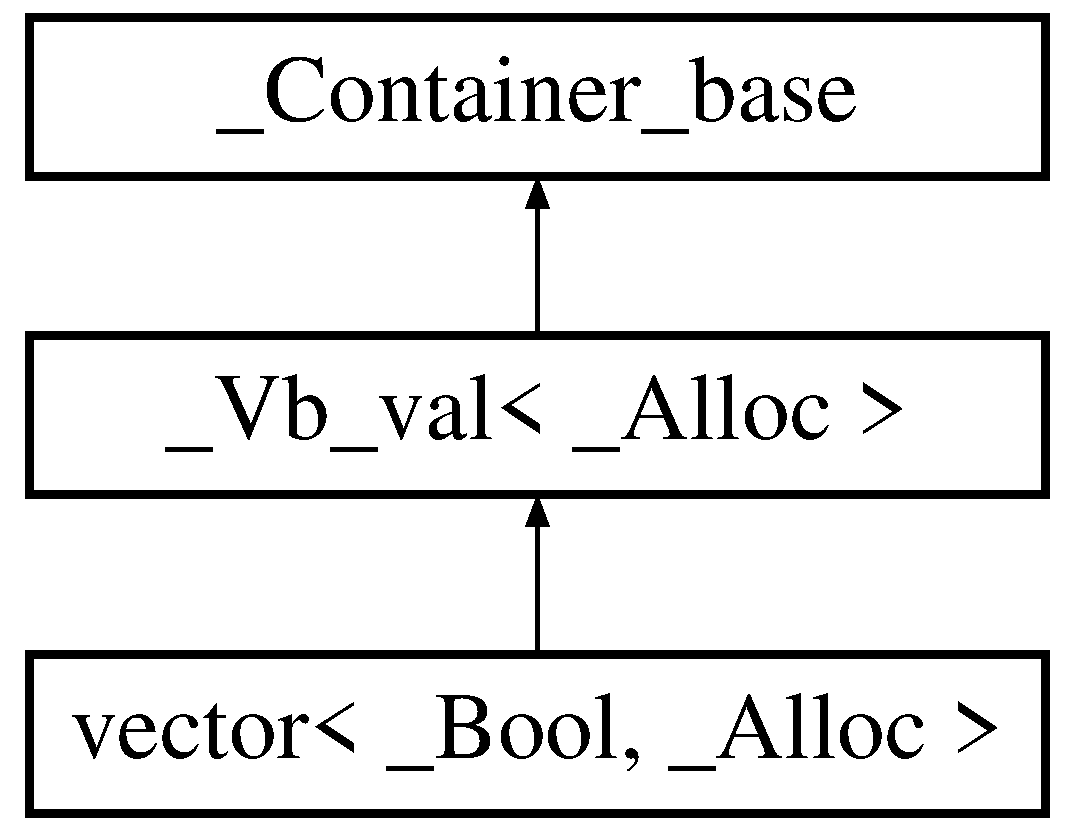
\includegraphics[height=3.000000cm]{class___vb__val}
\end{center}
\end{figure}
\subsection*{Public Types}
\begin{DoxyCompactItemize}
\item 
typedef \+\_\+\+Alloc\+::template \\*
rebind$<$ \hyperlink{vector_8h_a1555a2f621ba9ade75bb9ce8bca77144}{\+\_\+\+Vbase} $>$\+::other \hyperlink{class___vb__val_a20c01f1d8456573db64c3f9098bb5eda}{\+\_\+\+Alty}
\item 
typedef \+\_\+\+Alty\+::size\+\_\+type \hyperlink{class___vb__val_aae6aa10bcd41d235b46f128df1198612}{size\+\_\+type}
\end{DoxyCompactItemize}
\subsection*{Public Member Functions}
\begin{DoxyCompactItemize}
\item 
\hyperlink{class___vb__val_a40d7d702dcab7f7f8aa893263bf501ff}{\+\_\+\+Vb\+\_\+val} (\hyperlink{class___vb__val_aae6aa10bcd41d235b46f128df1198612}{size\+\_\+type} \+\_\+\+Count, bool \+\_\+\+Val, \+\_\+\+Alloc \+\_\+\+Al=\+\_\+\+Alloc())
\item 
\hyperlink{class___vb__val_a9c4e8432d643ca9239347b7d6fdb05ab}{$\sim$\+\_\+\+Vb\+\_\+val} ()
\end{DoxyCompactItemize}
\subsection*{Static Public Member Functions}
\begin{DoxyCompactItemize}
\item 
static \hyperlink{class___vb__val_aae6aa10bcd41d235b46f128df1198612}{size\+\_\+type} \hyperlink{class___vb__val_a4d2e656ee706fbd56939891618fa9057}{\+\_\+\+Nw} (\hyperlink{class___vb__val_aae6aa10bcd41d235b46f128df1198612}{size\+\_\+type} \+\_\+\+Count)
\end{DoxyCompactItemize}
\subsection*{Public Attributes}
\begin{DoxyCompactItemize}
\item 
\+\_\+\+S\+T\+D \hyperlink{classvector}{vector}$<$ \hyperlink{vector_8h_a1555a2f621ba9ade75bb9ce8bca77144}{\+\_\+\+Vbase}, \hyperlink{class___vb__val_a20c01f1d8456573db64c3f9098bb5eda}{\+\_\+\+Alty} $>$ \hyperlink{class___vb__val_a767a14d1ad38891dbf939ef319bab983}{\+\_\+\+Myvec}
\item 
\+\_\+\+Alty\+::size\+\_\+type \hyperlink{class___vb__val_accdd2cf575b73798e173b94f8c30dedc}{\+\_\+\+Mysize}
\end{DoxyCompactItemize}


\subsection{Detailed Description}
\subsubsection*{template$<$class \+\_\+\+Alloc$>$class \+\_\+\+Vb\+\_\+val$<$ \+\_\+\+Alloc $>$}



Definition at line 1999 of file vector.\+h.



\subsection{Member Typedef Documentation}
\hypertarget{class___vb__val_a20c01f1d8456573db64c3f9098bb5eda}{\index{\+\_\+\+Vb\+\_\+val@{\+\_\+\+Vb\+\_\+val}!\+\_\+\+Alty@{\+\_\+\+Alty}}
\index{\+\_\+\+Alty@{\+\_\+\+Alty}!\+\_\+\+Vb\+\_\+val@{\+\_\+\+Vb\+\_\+val}}
\subsubsection[{\+\_\+\+Alty}]{\setlength{\rightskip}{0pt plus 5cm}template$<$class \+\_\+\+Alloc $>$ typedef \+\_\+\+Alloc\+::template rebind$<${\bf \+\_\+\+Vbase}$>$\+::other {\bf \+\_\+\+Vb\+\_\+val}$<$ \+\_\+\+Alloc $>$\+::{\bf \+\_\+\+Alty}}}\label{class___vb__val_a20c01f1d8456573db64c3f9098bb5eda}


Definition at line 2003 of file vector.\+h.

\hypertarget{class___vb__val_aae6aa10bcd41d235b46f128df1198612}{\index{\+\_\+\+Vb\+\_\+val@{\+\_\+\+Vb\+\_\+val}!size\+\_\+type@{size\+\_\+type}}
\index{size\+\_\+type@{size\+\_\+type}!\+\_\+\+Vb\+\_\+val@{\+\_\+\+Vb\+\_\+val}}
\subsubsection[{size\+\_\+type}]{\setlength{\rightskip}{0pt plus 5cm}template$<$class \+\_\+\+Alloc $>$ typedef \+\_\+\+Alty\+::size\+\_\+type {\bf \+\_\+\+Vb\+\_\+val}$<$ \+\_\+\+Alloc $>$\+::{\bf size\+\_\+type}}}\label{class___vb__val_aae6aa10bcd41d235b46f128df1198612}


Definition at line 2004 of file vector.\+h.



\subsection{Constructor \& Destructor Documentation}
\hypertarget{class___vb__val_a40d7d702dcab7f7f8aa893263bf501ff}{\index{\+\_\+\+Vb\+\_\+val@{\+\_\+\+Vb\+\_\+val}!\+\_\+\+Vb\+\_\+val@{\+\_\+\+Vb\+\_\+val}}
\index{\+\_\+\+Vb\+\_\+val@{\+\_\+\+Vb\+\_\+val}!\+\_\+\+Vb\+\_\+val@{\+\_\+\+Vb\+\_\+val}}
\subsubsection[{\+\_\+\+Vb\+\_\+val}]{\setlength{\rightskip}{0pt plus 5cm}template$<$class \+\_\+\+Alloc $>$ {\bf \+\_\+\+Vb\+\_\+val}$<$ \+\_\+\+Alloc $>$\+::{\bf \+\_\+\+Vb\+\_\+val} (
\begin{DoxyParamCaption}
\item[{{\bf size\+\_\+type}}]{\+\_\+\+Count, }
\item[{bool}]{\+\_\+\+Val, }
\item[{\+\_\+\+Alloc}]{\+\_\+\+Al = {\ttfamily \+\_\+Alloc()}}
\end{DoxyParamCaption}
)\hspace{0.3cm}{\ttfamily [inline]}}}\label{class___vb__val_a40d7d702dcab7f7f8aa893263bf501ff}


Definition at line 2007 of file vector.\+h.

\hypertarget{class___vb__val_a9c4e8432d643ca9239347b7d6fdb05ab}{\index{\+\_\+\+Vb\+\_\+val@{\+\_\+\+Vb\+\_\+val}!````~\+\_\+\+Vb\+\_\+val@{$\sim$\+\_\+\+Vb\+\_\+val}}
\index{````~\+\_\+\+Vb\+\_\+val@{$\sim$\+\_\+\+Vb\+\_\+val}!\+\_\+\+Vb\+\_\+val@{\+\_\+\+Vb\+\_\+val}}
\subsubsection[{$\sim$\+\_\+\+Vb\+\_\+val}]{\setlength{\rightskip}{0pt plus 5cm}template$<$class \+\_\+\+Alloc $>$ {\bf \+\_\+\+Vb\+\_\+val}$<$ \+\_\+\+Alloc $>$\+::$\sim${\bf \+\_\+\+Vb\+\_\+val} (
\begin{DoxyParamCaption}
{}
\end{DoxyParamCaption}
)\hspace{0.3cm}{\ttfamily [inline]}}}\label{class___vb__val_a9c4e8432d643ca9239347b7d6fdb05ab}


Definition at line 2013 of file vector.\+h.



\subsection{Member Function Documentation}
\hypertarget{class___vb__val_a4d2e656ee706fbd56939891618fa9057}{\index{\+\_\+\+Vb\+\_\+val@{\+\_\+\+Vb\+\_\+val}!\+\_\+\+Nw@{\+\_\+\+Nw}}
\index{\+\_\+\+Nw@{\+\_\+\+Nw}!\+\_\+\+Vb\+\_\+val@{\+\_\+\+Vb\+\_\+val}}
\subsubsection[{\+\_\+\+Nw}]{\setlength{\rightskip}{0pt plus 5cm}template$<$class \+\_\+\+Alloc $>$ static {\bf size\+\_\+type} {\bf \+\_\+\+Vb\+\_\+val}$<$ \+\_\+\+Alloc $>$\+::\+\_\+\+Nw (
\begin{DoxyParamCaption}
\item[{{\bf size\+\_\+type}}]{\+\_\+\+Count}
\end{DoxyParamCaption}
)\hspace{0.3cm}{\ttfamily [inline]}, {\ttfamily [static]}}}\label{class___vb__val_a4d2e656ee706fbd56939891618fa9057}


Definition at line 2051 of file vector.\+h.



\subsection{Member Data Documentation}
\hypertarget{class___vb__val_accdd2cf575b73798e173b94f8c30dedc}{\index{\+\_\+\+Vb\+\_\+val@{\+\_\+\+Vb\+\_\+val}!\+\_\+\+Mysize@{\+\_\+\+Mysize}}
\index{\+\_\+\+Mysize@{\+\_\+\+Mysize}!\+\_\+\+Vb\+\_\+val@{\+\_\+\+Vb\+\_\+val}}
\subsubsection[{\+\_\+\+Mysize}]{\setlength{\rightskip}{0pt plus 5cm}template$<$class \+\_\+\+Alloc $>$ \+\_\+\+Alty\+::size\+\_\+type {\bf \+\_\+\+Vb\+\_\+val}$<$ \+\_\+\+Alloc $>$\+::\+\_\+\+Mysize}}\label{class___vb__val_accdd2cf575b73798e173b94f8c30dedc}


Definition at line 2057 of file vector.\+h.

\hypertarget{class___vb__val_a767a14d1ad38891dbf939ef319bab983}{\index{\+\_\+\+Vb\+\_\+val@{\+\_\+\+Vb\+\_\+val}!\+\_\+\+Myvec@{\+\_\+\+Myvec}}
\index{\+\_\+\+Myvec@{\+\_\+\+Myvec}!\+\_\+\+Vb\+\_\+val@{\+\_\+\+Vb\+\_\+val}}
\subsubsection[{\+\_\+\+Myvec}]{\setlength{\rightskip}{0pt plus 5cm}template$<$class \+\_\+\+Alloc $>$ \+\_\+\+S\+T\+D {\bf vector}$<${\bf \+\_\+\+Vbase}, {\bf \+\_\+\+Alty}$>$ {\bf \+\_\+\+Vb\+\_\+val}$<$ \+\_\+\+Alloc $>$\+::\+\_\+\+Myvec}}\label{class___vb__val_a767a14d1ad38891dbf939ef319bab983}


Definition at line 2056 of file vector.\+h.



The documentation for this class was generated from the following file\+:\begin{DoxyCompactItemize}
\item 
\hyperlink{vector_8h}{vector.\+h}\end{DoxyCompactItemize}

\hypertarget{class___vector__const__iterator}{\section{\+\_\+\+Vector\+\_\+const\+\_\+iterator$<$ \+\_\+\+Myvec $>$ Class Template Reference}
\label{class___vector__const__iterator}\index{\+\_\+\+Vector\+\_\+const\+\_\+iterator$<$ \+\_\+\+Myvec $>$@{\+\_\+\+Vector\+\_\+const\+\_\+iterator$<$ \+\_\+\+Myvec $>$}}
}


{\ttfamily \#include $<$vector.\+h$>$}

Inheritance diagram for \+\_\+\+Vector\+\_\+const\+\_\+iterator$<$ \+\_\+\+Myvec $>$\+:\begin{figure}[H]
\begin{center}
\leavevmode
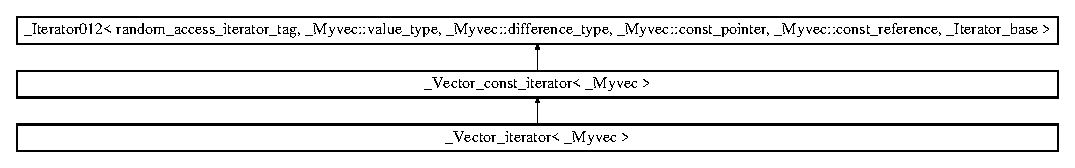
\includegraphics[height=1.814255cm]{class___vector__const__iterator}
\end{center}
\end{figure}
\subsection*{Public Types}
\begin{DoxyCompactItemize}
\item 
typedef \hyperlink{class___vector__const__iterator}{\+\_\+\+Vector\+\_\+const\+\_\+iterator}\\*
$<$ \+\_\+\+Myvec $>$ \hyperlink{class___vector__const__iterator_ac41cce1a95dfa665c2d7237fd94d776b}{\+\_\+\+Myiter}
\item 
typedef random\+\_\+access\+\_\+iterator\+\_\+tag \hyperlink{class___vector__const__iterator_a3e45b76a1bb5d1c6adb70bf8d924d1e5}{iterator\+\_\+category}
\item 
typedef \+\_\+\+Myvec\+::pointer \hyperlink{class___vector__const__iterator_a9b6960b4fe0656e2e83c54e6c7757a15}{\+\_\+\+Tptr}
\item 
typedef \+\_\+\+Myvec\+::value\+\_\+type \hyperlink{class___vector__const__iterator_ae488763bcaee2e0738351caacc5c8922}{value\+\_\+type}
\item 
typedef \+\_\+\+Myvec\+::difference\+\_\+type \hyperlink{class___vector__const__iterator_a4fad8668028c0db06eda92c190eeca39}{difference\+\_\+type}
\item 
typedef \+\_\+\+Myvec\+::const\+\_\+pointer \hyperlink{class___vector__const__iterator_a301a1187c227c820bd86335496229e6a}{pointer}
\item 
typedef \+\_\+\+Myvec\+::const\+\_\+reference \hyperlink{class___vector__const__iterator_ad622d2f855c02a5b3b2f49f39cbbabf4}{reference}
\item 
typedef \hyperlink{class___vector__const__iterator_a301a1187c227c820bd86335496229e6a}{pointer} \hyperlink{class___vector__const__iterator_a17897ed20e5a6c25f9b383d0f0a4bb9d}{\+\_\+\+Unchecked\+\_\+type}
\end{DoxyCompactItemize}
\subsection*{Public Member Functions}
\begin{DoxyCompactItemize}
\item 
\hyperlink{class___vector__const__iterator_abe1aa8a2e93616a96b68fba5d20840c0}{\+\_\+\+Vector\+\_\+const\+\_\+iterator} ()
\item 
\hyperlink{class___vector__const__iterator_ae032c3d3a887e78738ff28dfaeeafc09}{\+\_\+\+Vector\+\_\+const\+\_\+iterator} (\hyperlink{class___vector__const__iterator_a9b6960b4fe0656e2e83c54e6c7757a15}{\+\_\+\+Tptr} \+\_\+\+Parg, const \+\_\+\+Container\+\_\+base $\ast$\+\_\+\+Pvector)
\item 
\hyperlink{class___vector__const__iterator_ac41cce1a95dfa665c2d7237fd94d776b}{\+\_\+\+Myiter} \& \hyperlink{class___vector__const__iterator_a1efb4c8566f4ed31eb665c65cc74d1dc}{\+\_\+\+Rechecked} (\hyperlink{class___vector__const__iterator_a17897ed20e5a6c25f9b383d0f0a4bb9d}{\+\_\+\+Unchecked\+\_\+type} \+\_\+\+Right)
\item 
\hyperlink{class___vector__const__iterator_a17897ed20e5a6c25f9b383d0f0a4bb9d}{\+\_\+\+Unchecked\+\_\+type} \hyperlink{class___vector__const__iterator_a0f1bb188a364ea983f766cd7cb08a1d8}{\+\_\+\+Unchecked} () const 
\item 
\hyperlink{class___vector__const__iterator_ad622d2f855c02a5b3b2f49f39cbbabf4}{reference} \hyperlink{class___vector__const__iterator_aff78225a996909556ae7836840592bec}{operator$\ast$} () const 
\item 
\hyperlink{class___vector__const__iterator_a301a1187c227c820bd86335496229e6a}{pointer} \hyperlink{class___vector__const__iterator_aff1b4b3863ccd8d605288acd0bdab017}{operator-\/$>$} () const 
\item 
\hyperlink{class___vector__const__iterator_ac41cce1a95dfa665c2d7237fd94d776b}{\+\_\+\+Myiter} \& \hyperlink{class___vector__const__iterator_af06aa214fc08cfe0a52f1cade5e11297}{operator++} ()
\item 
\hyperlink{class___vector__const__iterator_ac41cce1a95dfa665c2d7237fd94d776b}{\+\_\+\+Myiter} \hyperlink{class___vector__const__iterator_ab85d07f8d450f7a039f3718e2fa40085}{operator++} (int)
\item 
\hyperlink{class___vector__const__iterator_ac41cce1a95dfa665c2d7237fd94d776b}{\+\_\+\+Myiter} \& \hyperlink{class___vector__const__iterator_a308a1e2758c025af89d9827611991f75}{operator-\/-\/} ()
\item 
\hyperlink{class___vector__const__iterator_ac41cce1a95dfa665c2d7237fd94d776b}{\+\_\+\+Myiter} \hyperlink{class___vector__const__iterator_abbb7cfe7ce38c5adbb20b0fa0892a746}{operator-\/-\/} (int)
\item 
\hyperlink{class___vector__const__iterator_ac41cce1a95dfa665c2d7237fd94d776b}{\+\_\+\+Myiter} \& \hyperlink{class___vector__const__iterator_affaf0a330a883ac3f9595d6c94587e42}{operator+=} (\hyperlink{class___vector__const__iterator_a4fad8668028c0db06eda92c190eeca39}{difference\+\_\+type} \+\_\+\+Off)
\item 
\hyperlink{class___vector__const__iterator_ac41cce1a95dfa665c2d7237fd94d776b}{\+\_\+\+Myiter} \hyperlink{class___vector__const__iterator_a657a041e6acfd3e27e29aad419951ca2}{operator+} (\hyperlink{class___vector__const__iterator_a4fad8668028c0db06eda92c190eeca39}{difference\+\_\+type} \+\_\+\+Off) const 
\item 
\hyperlink{class___vector__const__iterator_ac41cce1a95dfa665c2d7237fd94d776b}{\+\_\+\+Myiter} \& \hyperlink{class___vector__const__iterator_a1a1b12bf78c271d6832240b801554204}{operator-\/=} (\hyperlink{class___vector__const__iterator_a4fad8668028c0db06eda92c190eeca39}{difference\+\_\+type} \+\_\+\+Off)
\item 
\hyperlink{class___vector__const__iterator_ac41cce1a95dfa665c2d7237fd94d776b}{\+\_\+\+Myiter} \hyperlink{class___vector__const__iterator_ad45f9e7dde0a0bfa1fc8f1c3711d0447}{operator-\/} (\hyperlink{class___vector__const__iterator_a4fad8668028c0db06eda92c190eeca39}{difference\+\_\+type} \+\_\+\+Off) const 
\item 
\hyperlink{class___vector__const__iterator_a4fad8668028c0db06eda92c190eeca39}{difference\+\_\+type} \hyperlink{class___vector__const__iterator_a633f3e03af0ba527fc80454629f34c7e}{operator-\/} (const \hyperlink{class___vector__const__iterator_ac41cce1a95dfa665c2d7237fd94d776b}{\+\_\+\+Myiter} \&\+\_\+\+Right) const 
\item 
\hyperlink{class___vector__const__iterator_ad622d2f855c02a5b3b2f49f39cbbabf4}{reference} \hyperlink{class___vector__const__iterator_a89e06ec06f88dc4897da3793c3aa19b9}{operator\mbox{[}$\,$\mbox{]}} (\hyperlink{class___vector__const__iterator_a4fad8668028c0db06eda92c190eeca39}{difference\+\_\+type} \+\_\+\+Off) const 
\item 
bool \hyperlink{class___vector__const__iterator_adac14f68d59d3b96c7211b4e35dee0bc}{operator==} (const \hyperlink{class___vector__const__iterator_ac41cce1a95dfa665c2d7237fd94d776b}{\+\_\+\+Myiter} \&\+\_\+\+Right) const 
\item 
bool \hyperlink{class___vector__const__iterator_ad39d47fe82c1c1dd61f3b507acedc13e}{operator!=} (const \hyperlink{class___vector__const__iterator_ac41cce1a95dfa665c2d7237fd94d776b}{\+\_\+\+Myiter} \&\+\_\+\+Right) const 
\item 
bool \hyperlink{class___vector__const__iterator_a9828845596ea577cd18ac917d4bf6ada}{operator$<$} (const \hyperlink{class___vector__const__iterator_ac41cce1a95dfa665c2d7237fd94d776b}{\+\_\+\+Myiter} \&\+\_\+\+Right) const 
\item 
bool \hyperlink{class___vector__const__iterator_a41bf77cee70e02ea7043aeafc5f52feb}{operator$>$} (const \hyperlink{class___vector__const__iterator_ac41cce1a95dfa665c2d7237fd94d776b}{\+\_\+\+Myiter} \&\+\_\+\+Right) const 
\item 
bool \hyperlink{class___vector__const__iterator_af6d151eed7372fb887708802fc016083}{operator$<$=} (const \hyperlink{class___vector__const__iterator_ac41cce1a95dfa665c2d7237fd94d776b}{\+\_\+\+Myiter} \&\+\_\+\+Right) const 
\item 
bool \hyperlink{class___vector__const__iterator_aa5eabf17e130fe96933e2035f8eac7bd}{operator$>$=} (const \hyperlink{class___vector__const__iterator_ac41cce1a95dfa665c2d7237fd94d776b}{\+\_\+\+Myiter} \&\+\_\+\+Right) const 
\item 
void \hyperlink{class___vector__const__iterator_afd73ab744b74a3fe26c9857a287f038e}{\+\_\+\+Compat} (const \hyperlink{class___vector__const__iterator_ac41cce1a95dfa665c2d7237fd94d776b}{\+\_\+\+Myiter} \&) const 
\end{DoxyCompactItemize}
\subsection*{Public Attributes}
\begin{DoxyCompactItemize}
\item 
\hyperlink{class___vector__const__iterator_a9b6960b4fe0656e2e83c54e6c7757a15}{\+\_\+\+Tptr} \hyperlink{class___vector__const__iterator_a4671fc4a9c2824046f5a827afb87b721}{\+\_\+\+Ptr}
\end{DoxyCompactItemize}


\subsection{Detailed Description}
\subsubsection*{template$<$class \+\_\+\+Myvec$>$class \+\_\+\+Vector\+\_\+const\+\_\+iterator$<$ \+\_\+\+Myvec $>$}



Definition at line 20 of file vector.\+h.



\subsection{Member Typedef Documentation}
\hypertarget{class___vector__const__iterator_ac41cce1a95dfa665c2d7237fd94d776b}{\index{\+\_\+\+Vector\+\_\+const\+\_\+iterator@{\+\_\+\+Vector\+\_\+const\+\_\+iterator}!\+\_\+\+Myiter@{\+\_\+\+Myiter}}
\index{\+\_\+\+Myiter@{\+\_\+\+Myiter}!\+\_\+\+Vector\+\_\+const\+\_\+iterator@{\+\_\+\+Vector\+\_\+const\+\_\+iterator}}
\subsubsection[{\+\_\+\+Myiter}]{\setlength{\rightskip}{0pt plus 5cm}template$<$class \+\_\+\+Myvec$>$ typedef {\bf \+\_\+\+Vector\+\_\+const\+\_\+iterator}$<$\+\_\+\+Myvec$>$ {\bf \+\_\+\+Vector\+\_\+const\+\_\+iterator}$<$ \+\_\+\+Myvec $>$\+::{\bf \+\_\+\+Myiter}}}\label{class___vector__const__iterator_ac41cce1a95dfa665c2d7237fd94d776b}


Definition at line 29 of file vector.\+h.

\hypertarget{class___vector__const__iterator_a9b6960b4fe0656e2e83c54e6c7757a15}{\index{\+\_\+\+Vector\+\_\+const\+\_\+iterator@{\+\_\+\+Vector\+\_\+const\+\_\+iterator}!\+\_\+\+Tptr@{\+\_\+\+Tptr}}
\index{\+\_\+\+Tptr@{\+\_\+\+Tptr}!\+\_\+\+Vector\+\_\+const\+\_\+iterator@{\+\_\+\+Vector\+\_\+const\+\_\+iterator}}
\subsubsection[{\+\_\+\+Tptr}]{\setlength{\rightskip}{0pt plus 5cm}template$<$class \+\_\+\+Myvec$>$ typedef \+\_\+\+Myvec\+::pointer {\bf \+\_\+\+Vector\+\_\+const\+\_\+iterator}$<$ \+\_\+\+Myvec $>$\+::{\bf \+\_\+\+Tptr}}}\label{class___vector__const__iterator_a9b6960b4fe0656e2e83c54e6c7757a15}


Definition at line 32 of file vector.\+h.

\hypertarget{class___vector__const__iterator_a17897ed20e5a6c25f9b383d0f0a4bb9d}{\index{\+\_\+\+Vector\+\_\+const\+\_\+iterator@{\+\_\+\+Vector\+\_\+const\+\_\+iterator}!\+\_\+\+Unchecked\+\_\+type@{\+\_\+\+Unchecked\+\_\+type}}
\index{\+\_\+\+Unchecked\+\_\+type@{\+\_\+\+Unchecked\+\_\+type}!\+\_\+\+Vector\+\_\+const\+\_\+iterator@{\+\_\+\+Vector\+\_\+const\+\_\+iterator}}
\subsubsection[{\+\_\+\+Unchecked\+\_\+type}]{\setlength{\rightskip}{0pt plus 5cm}template$<$class \+\_\+\+Myvec$>$ typedef {\bf pointer} {\bf \+\_\+\+Vector\+\_\+const\+\_\+iterator}$<$ \+\_\+\+Myvec $>$\+::{\bf \+\_\+\+Unchecked\+\_\+type}}}\label{class___vector__const__iterator_a17897ed20e5a6c25f9b383d0f0a4bb9d}


Definition at line 49 of file vector.\+h.

\hypertarget{class___vector__const__iterator_a4fad8668028c0db06eda92c190eeca39}{\index{\+\_\+\+Vector\+\_\+const\+\_\+iterator@{\+\_\+\+Vector\+\_\+const\+\_\+iterator}!difference\+\_\+type@{difference\+\_\+type}}
\index{difference\+\_\+type@{difference\+\_\+type}!\+\_\+\+Vector\+\_\+const\+\_\+iterator@{\+\_\+\+Vector\+\_\+const\+\_\+iterator}}
\subsubsection[{difference\+\_\+type}]{\setlength{\rightskip}{0pt plus 5cm}template$<$class \+\_\+\+Myvec$>$ typedef \+\_\+\+Myvec\+::difference\+\_\+type {\bf \+\_\+\+Vector\+\_\+const\+\_\+iterator}$<$ \+\_\+\+Myvec $>$\+::{\bf difference\+\_\+type}}}\label{class___vector__const__iterator_a4fad8668028c0db06eda92c190eeca39}


Definition at line 34 of file vector.\+h.

\hypertarget{class___vector__const__iterator_a3e45b76a1bb5d1c6adb70bf8d924d1e5}{\index{\+\_\+\+Vector\+\_\+const\+\_\+iterator@{\+\_\+\+Vector\+\_\+const\+\_\+iterator}!iterator\+\_\+category@{iterator\+\_\+category}}
\index{iterator\+\_\+category@{iterator\+\_\+category}!\+\_\+\+Vector\+\_\+const\+\_\+iterator@{\+\_\+\+Vector\+\_\+const\+\_\+iterator}}
\subsubsection[{iterator\+\_\+category}]{\setlength{\rightskip}{0pt plus 5cm}template$<$class \+\_\+\+Myvec$>$ typedef random\+\_\+access\+\_\+iterator\+\_\+tag {\bf \+\_\+\+Vector\+\_\+const\+\_\+iterator}$<$ \+\_\+\+Myvec $>$\+::{\bf iterator\+\_\+category}}}\label{class___vector__const__iterator_a3e45b76a1bb5d1c6adb70bf8d924d1e5}


Definition at line 30 of file vector.\+h.

\hypertarget{class___vector__const__iterator_a301a1187c227c820bd86335496229e6a}{\index{\+\_\+\+Vector\+\_\+const\+\_\+iterator@{\+\_\+\+Vector\+\_\+const\+\_\+iterator}!pointer@{pointer}}
\index{pointer@{pointer}!\+\_\+\+Vector\+\_\+const\+\_\+iterator@{\+\_\+\+Vector\+\_\+const\+\_\+iterator}}
\subsubsection[{pointer}]{\setlength{\rightskip}{0pt plus 5cm}template$<$class \+\_\+\+Myvec$>$ typedef \+\_\+\+Myvec\+::const\+\_\+pointer {\bf \+\_\+\+Vector\+\_\+const\+\_\+iterator}$<$ \+\_\+\+Myvec $>$\+::{\bf pointer}}}\label{class___vector__const__iterator_a301a1187c227c820bd86335496229e6a}


Definition at line 35 of file vector.\+h.

\hypertarget{class___vector__const__iterator_ad622d2f855c02a5b3b2f49f39cbbabf4}{\index{\+\_\+\+Vector\+\_\+const\+\_\+iterator@{\+\_\+\+Vector\+\_\+const\+\_\+iterator}!reference@{reference}}
\index{reference@{reference}!\+\_\+\+Vector\+\_\+const\+\_\+iterator@{\+\_\+\+Vector\+\_\+const\+\_\+iterator}}
\subsubsection[{reference}]{\setlength{\rightskip}{0pt plus 5cm}template$<$class \+\_\+\+Myvec$>$ typedef \+\_\+\+Myvec\+::const\+\_\+reference {\bf \+\_\+\+Vector\+\_\+const\+\_\+iterator}$<$ \+\_\+\+Myvec $>$\+::{\bf reference}}}\label{class___vector__const__iterator_ad622d2f855c02a5b3b2f49f39cbbabf4}


Definition at line 36 of file vector.\+h.

\hypertarget{class___vector__const__iterator_ae488763bcaee2e0738351caacc5c8922}{\index{\+\_\+\+Vector\+\_\+const\+\_\+iterator@{\+\_\+\+Vector\+\_\+const\+\_\+iterator}!value\+\_\+type@{value\+\_\+type}}
\index{value\+\_\+type@{value\+\_\+type}!\+\_\+\+Vector\+\_\+const\+\_\+iterator@{\+\_\+\+Vector\+\_\+const\+\_\+iterator}}
\subsubsection[{value\+\_\+type}]{\setlength{\rightskip}{0pt plus 5cm}template$<$class \+\_\+\+Myvec$>$ typedef \+\_\+\+Myvec\+::value\+\_\+type {\bf \+\_\+\+Vector\+\_\+const\+\_\+iterator}$<$ \+\_\+\+Myvec $>$\+::{\bf value\+\_\+type}}}\label{class___vector__const__iterator_ae488763bcaee2e0738351caacc5c8922}


Definition at line 33 of file vector.\+h.



\subsection{Constructor \& Destructor Documentation}
\hypertarget{class___vector__const__iterator_abe1aa8a2e93616a96b68fba5d20840c0}{\index{\+\_\+\+Vector\+\_\+const\+\_\+iterator@{\+\_\+\+Vector\+\_\+const\+\_\+iterator}!\+\_\+\+Vector\+\_\+const\+\_\+iterator@{\+\_\+\+Vector\+\_\+const\+\_\+iterator}}
\index{\+\_\+\+Vector\+\_\+const\+\_\+iterator@{\+\_\+\+Vector\+\_\+const\+\_\+iterator}!\+\_\+\+Vector\+\_\+const\+\_\+iterator@{\+\_\+\+Vector\+\_\+const\+\_\+iterator}}
\subsubsection[{\+\_\+\+Vector\+\_\+const\+\_\+iterator}]{\setlength{\rightskip}{0pt plus 5cm}template$<$class \+\_\+\+Myvec$>$ {\bf \+\_\+\+Vector\+\_\+const\+\_\+iterator}$<$ \+\_\+\+Myvec $>$\+::{\bf \+\_\+\+Vector\+\_\+const\+\_\+iterator} (
\begin{DoxyParamCaption}
{}
\end{DoxyParamCaption}
)\hspace{0.3cm}{\ttfamily [inline]}}}\label{class___vector__const__iterator_abe1aa8a2e93616a96b68fba5d20840c0}


Definition at line 38 of file vector.\+h.

\hypertarget{class___vector__const__iterator_ae032c3d3a887e78738ff28dfaeeafc09}{\index{\+\_\+\+Vector\+\_\+const\+\_\+iterator@{\+\_\+\+Vector\+\_\+const\+\_\+iterator}!\+\_\+\+Vector\+\_\+const\+\_\+iterator@{\+\_\+\+Vector\+\_\+const\+\_\+iterator}}
\index{\+\_\+\+Vector\+\_\+const\+\_\+iterator@{\+\_\+\+Vector\+\_\+const\+\_\+iterator}!\+\_\+\+Vector\+\_\+const\+\_\+iterator@{\+\_\+\+Vector\+\_\+const\+\_\+iterator}}
\subsubsection[{\+\_\+\+Vector\+\_\+const\+\_\+iterator}]{\setlength{\rightskip}{0pt plus 5cm}template$<$class \+\_\+\+Myvec$>$ {\bf \+\_\+\+Vector\+\_\+const\+\_\+iterator}$<$ \+\_\+\+Myvec $>$\+::{\bf \+\_\+\+Vector\+\_\+const\+\_\+iterator} (
\begin{DoxyParamCaption}
\item[{{\bf \+\_\+\+Tptr}}]{\+\_\+\+Parg, }
\item[{const \+\_\+\+Container\+\_\+base $\ast$}]{\+\_\+\+Pvector}
\end{DoxyParamCaption}
)\hspace{0.3cm}{\ttfamily [inline]}}}\label{class___vector__const__iterator_ae032c3d3a887e78738ff28dfaeeafc09}


Definition at line 43 of file vector.\+h.



\subsection{Member Function Documentation}
\hypertarget{class___vector__const__iterator_afd73ab744b74a3fe26c9857a287f038e}{\index{\+\_\+\+Vector\+\_\+const\+\_\+iterator@{\+\_\+\+Vector\+\_\+const\+\_\+iterator}!\+\_\+\+Compat@{\+\_\+\+Compat}}
\index{\+\_\+\+Compat@{\+\_\+\+Compat}!\+\_\+\+Vector\+\_\+const\+\_\+iterator@{\+\_\+\+Vector\+\_\+const\+\_\+iterator}}
\subsubsection[{\+\_\+\+Compat}]{\setlength{\rightskip}{0pt plus 5cm}template$<$class \+\_\+\+Myvec$>$ void {\bf \+\_\+\+Vector\+\_\+const\+\_\+iterator}$<$ \+\_\+\+Myvec $>$\+::\+\_\+\+Compat (
\begin{DoxyParamCaption}
\item[{const {\bf \+\_\+\+Myiter} \&}]{}
\end{DoxyParamCaption}
) const\hspace{0.3cm}{\ttfamily [inline]}}}\label{class___vector__const__iterator_afd73ab744b74a3fe26c9857a287f038e}


Definition at line 251 of file vector.\+h.

\hypertarget{class___vector__const__iterator_a1efb4c8566f4ed31eb665c65cc74d1dc}{\index{\+\_\+\+Vector\+\_\+const\+\_\+iterator@{\+\_\+\+Vector\+\_\+const\+\_\+iterator}!\+\_\+\+Rechecked@{\+\_\+\+Rechecked}}
\index{\+\_\+\+Rechecked@{\+\_\+\+Rechecked}!\+\_\+\+Vector\+\_\+const\+\_\+iterator@{\+\_\+\+Vector\+\_\+const\+\_\+iterator}}
\subsubsection[{\+\_\+\+Rechecked}]{\setlength{\rightskip}{0pt plus 5cm}template$<$class \+\_\+\+Myvec$>$ {\bf \+\_\+\+Myiter}\& {\bf \+\_\+\+Vector\+\_\+const\+\_\+iterator}$<$ \+\_\+\+Myvec $>$\+::\+\_\+\+Rechecked (
\begin{DoxyParamCaption}
\item[{{\bf \+\_\+\+Unchecked\+\_\+type}}]{\+\_\+\+Right}
\end{DoxyParamCaption}
)\hspace{0.3cm}{\ttfamily [inline]}}}\label{class___vector__const__iterator_a1efb4c8566f4ed31eb665c65cc74d1dc}


Definition at line 51 of file vector.\+h.

\hypertarget{class___vector__const__iterator_a0f1bb188a364ea983f766cd7cb08a1d8}{\index{\+\_\+\+Vector\+\_\+const\+\_\+iterator@{\+\_\+\+Vector\+\_\+const\+\_\+iterator}!\+\_\+\+Unchecked@{\+\_\+\+Unchecked}}
\index{\+\_\+\+Unchecked@{\+\_\+\+Unchecked}!\+\_\+\+Vector\+\_\+const\+\_\+iterator@{\+\_\+\+Vector\+\_\+const\+\_\+iterator}}
\subsubsection[{\+\_\+\+Unchecked}]{\setlength{\rightskip}{0pt plus 5cm}template$<$class \+\_\+\+Myvec$>$ {\bf \+\_\+\+Unchecked\+\_\+type} {\bf \+\_\+\+Vector\+\_\+const\+\_\+iterator}$<$ \+\_\+\+Myvec $>$\+::\+\_\+\+Unchecked (
\begin{DoxyParamCaption}
{}
\end{DoxyParamCaption}
) const\hspace{0.3cm}{\ttfamily [inline]}}}\label{class___vector__const__iterator_a0f1bb188a364ea983f766cd7cb08a1d8}


Definition at line 57 of file vector.\+h.

\hypertarget{class___vector__const__iterator_ad39d47fe82c1c1dd61f3b507acedc13e}{\index{\+\_\+\+Vector\+\_\+const\+\_\+iterator@{\+\_\+\+Vector\+\_\+const\+\_\+iterator}!operator"!=@{operator"!=}}
\index{operator"!=@{operator"!=}!\+\_\+\+Vector\+\_\+const\+\_\+iterator@{\+\_\+\+Vector\+\_\+const\+\_\+iterator}}
\subsubsection[{operator"!=}]{\setlength{\rightskip}{0pt plus 5cm}template$<$class \+\_\+\+Myvec$>$ bool {\bf \+\_\+\+Vector\+\_\+const\+\_\+iterator}$<$ \+\_\+\+Myvec $>$\+::operator!= (
\begin{DoxyParamCaption}
\item[{const {\bf \+\_\+\+Myiter} \&}]{\+\_\+\+Right}
\end{DoxyParamCaption}
) const\hspace{0.3cm}{\ttfamily [inline]}}}\label{class___vector__const__iterator_ad39d47fe82c1c1dd61f3b507acedc13e}


Definition at line 206 of file vector.\+h.

\hypertarget{class___vector__const__iterator_aff78225a996909556ae7836840592bec}{\index{\+\_\+\+Vector\+\_\+const\+\_\+iterator@{\+\_\+\+Vector\+\_\+const\+\_\+iterator}!operator$\ast$@{operator$\ast$}}
\index{operator$\ast$@{operator$\ast$}!\+\_\+\+Vector\+\_\+const\+\_\+iterator@{\+\_\+\+Vector\+\_\+const\+\_\+iterator}}
\subsubsection[{operator$\ast$}]{\setlength{\rightskip}{0pt plus 5cm}template$<$class \+\_\+\+Myvec$>$ {\bf reference} {\bf \+\_\+\+Vector\+\_\+const\+\_\+iterator}$<$ \+\_\+\+Myvec $>$\+::operator$\ast$ (
\begin{DoxyParamCaption}
{}
\end{DoxyParamCaption}
) const\hspace{0.3cm}{\ttfamily [inline]}}}\label{class___vector__const__iterator_aff78225a996909556ae7836840592bec}


Definition at line 62 of file vector.\+h.

\hypertarget{class___vector__const__iterator_a657a041e6acfd3e27e29aad419951ca2}{\index{\+\_\+\+Vector\+\_\+const\+\_\+iterator@{\+\_\+\+Vector\+\_\+const\+\_\+iterator}!operator+@{operator+}}
\index{operator+@{operator+}!\+\_\+\+Vector\+\_\+const\+\_\+iterator@{\+\_\+\+Vector\+\_\+const\+\_\+iterator}}
\subsubsection[{operator+}]{\setlength{\rightskip}{0pt plus 5cm}template$<$class \+\_\+\+Myvec$>$ {\bf \+\_\+\+Myiter} {\bf \+\_\+\+Vector\+\_\+const\+\_\+iterator}$<$ \+\_\+\+Myvec $>$\+::operator+ (
\begin{DoxyParamCaption}
\item[{{\bf difference\+\_\+type}}]{\+\_\+\+Off}
\end{DoxyParamCaption}
) const\hspace{0.3cm}{\ttfamily [inline]}}}\label{class___vector__const__iterator_a657a041e6acfd3e27e29aad419951ca2}


Definition at line 172 of file vector.\+h.

\hypertarget{class___vector__const__iterator_af06aa214fc08cfe0a52f1cade5e11297}{\index{\+\_\+\+Vector\+\_\+const\+\_\+iterator@{\+\_\+\+Vector\+\_\+const\+\_\+iterator}!operator++@{operator++}}
\index{operator++@{operator++}!\+\_\+\+Vector\+\_\+const\+\_\+iterator@{\+\_\+\+Vector\+\_\+const\+\_\+iterator}}
\subsubsection[{operator++}]{\setlength{\rightskip}{0pt plus 5cm}template$<$class \+\_\+\+Myvec$>$ {\bf \+\_\+\+Myiter}\& {\bf \+\_\+\+Vector\+\_\+const\+\_\+iterator}$<$ \+\_\+\+Myvec $>$\+::operator++ (
\begin{DoxyParamCaption}
{}
\end{DoxyParamCaption}
)\hspace{0.3cm}{\ttfamily [inline]}}}\label{class___vector__const__iterator_af06aa214fc08cfe0a52f1cade5e11297}


Definition at line 92 of file vector.\+h.

\hypertarget{class___vector__const__iterator_ab85d07f8d450f7a039f3718e2fa40085}{\index{\+\_\+\+Vector\+\_\+const\+\_\+iterator@{\+\_\+\+Vector\+\_\+const\+\_\+iterator}!operator++@{operator++}}
\index{operator++@{operator++}!\+\_\+\+Vector\+\_\+const\+\_\+iterator@{\+\_\+\+Vector\+\_\+const\+\_\+iterator}}
\subsubsection[{operator++}]{\setlength{\rightskip}{0pt plus 5cm}template$<$class \+\_\+\+Myvec$>$ {\bf \+\_\+\+Myiter} {\bf \+\_\+\+Vector\+\_\+const\+\_\+iterator}$<$ \+\_\+\+Myvec $>$\+::operator++ (
\begin{DoxyParamCaption}
\item[{int}]{}
\end{DoxyParamCaption}
)\hspace{0.3cm}{\ttfamily [inline]}}}\label{class___vector__const__iterator_ab85d07f8d450f7a039f3718e2fa40085}


Definition at line 114 of file vector.\+h.

\hypertarget{class___vector__const__iterator_affaf0a330a883ac3f9595d6c94587e42}{\index{\+\_\+\+Vector\+\_\+const\+\_\+iterator@{\+\_\+\+Vector\+\_\+const\+\_\+iterator}!operator+=@{operator+=}}
\index{operator+=@{operator+=}!\+\_\+\+Vector\+\_\+const\+\_\+iterator@{\+\_\+\+Vector\+\_\+const\+\_\+iterator}}
\subsubsection[{operator+=}]{\setlength{\rightskip}{0pt plus 5cm}template$<$class \+\_\+\+Myvec$>$ {\bf \+\_\+\+Myiter}\& {\bf \+\_\+\+Vector\+\_\+const\+\_\+iterator}$<$ \+\_\+\+Myvec $>$\+::operator+= (
\begin{DoxyParamCaption}
\item[{{\bf difference\+\_\+type}}]{\+\_\+\+Off}
\end{DoxyParamCaption}
)\hspace{0.3cm}{\ttfamily [inline]}}}\label{class___vector__const__iterator_affaf0a330a883ac3f9595d6c94587e42}


Definition at line 150 of file vector.\+h.

\hypertarget{class___vector__const__iterator_ad45f9e7dde0a0bfa1fc8f1c3711d0447}{\index{\+\_\+\+Vector\+\_\+const\+\_\+iterator@{\+\_\+\+Vector\+\_\+const\+\_\+iterator}!operator-\/@{operator-\/}}
\index{operator-\/@{operator-\/}!\+\_\+\+Vector\+\_\+const\+\_\+iterator@{\+\_\+\+Vector\+\_\+const\+\_\+iterator}}
\subsubsection[{operator-\/}]{\setlength{\rightskip}{0pt plus 5cm}template$<$class \+\_\+\+Myvec$>$ {\bf \+\_\+\+Myiter} {\bf \+\_\+\+Vector\+\_\+const\+\_\+iterator}$<$ \+\_\+\+Myvec $>$\+::operator-\/ (
\begin{DoxyParamCaption}
\item[{{\bf difference\+\_\+type}}]{\+\_\+\+Off}
\end{DoxyParamCaption}
) const\hspace{0.3cm}{\ttfamily [inline]}}}\label{class___vector__const__iterator_ad45f9e7dde0a0bfa1fc8f1c3711d0447}


Definition at line 183 of file vector.\+h.

\hypertarget{class___vector__const__iterator_a633f3e03af0ba527fc80454629f34c7e}{\index{\+\_\+\+Vector\+\_\+const\+\_\+iterator@{\+\_\+\+Vector\+\_\+const\+\_\+iterator}!operator-\/@{operator-\/}}
\index{operator-\/@{operator-\/}!\+\_\+\+Vector\+\_\+const\+\_\+iterator@{\+\_\+\+Vector\+\_\+const\+\_\+iterator}}
\subsubsection[{operator-\/}]{\setlength{\rightskip}{0pt plus 5cm}template$<$class \+\_\+\+Myvec$>$ {\bf difference\+\_\+type} {\bf \+\_\+\+Vector\+\_\+const\+\_\+iterator}$<$ \+\_\+\+Myvec $>$\+::operator-\/ (
\begin{DoxyParamCaption}
\item[{const {\bf \+\_\+\+Myiter} \&}]{\+\_\+\+Right}
\end{DoxyParamCaption}
) const\hspace{0.3cm}{\ttfamily [inline]}}}\label{class___vector__const__iterator_a633f3e03af0ba527fc80454629f34c7e}


Definition at line 189 of file vector.\+h.

\hypertarget{class___vector__const__iterator_a308a1e2758c025af89d9827611991f75}{\index{\+\_\+\+Vector\+\_\+const\+\_\+iterator@{\+\_\+\+Vector\+\_\+const\+\_\+iterator}!operator-\/-\/@{operator-\/-\/}}
\index{operator-\/-\/@{operator-\/-\/}!\+\_\+\+Vector\+\_\+const\+\_\+iterator@{\+\_\+\+Vector\+\_\+const\+\_\+iterator}}
\subsubsection[{operator-\/-\/}]{\setlength{\rightskip}{0pt plus 5cm}template$<$class \+\_\+\+Myvec$>$ {\bf \+\_\+\+Myiter}\& {\bf \+\_\+\+Vector\+\_\+const\+\_\+iterator}$<$ \+\_\+\+Myvec $>$\+::operator-\/-\/ (
\begin{DoxyParamCaption}
{}
\end{DoxyParamCaption}
)\hspace{0.3cm}{\ttfamily [inline]}}}\label{class___vector__const__iterator_a308a1e2758c025af89d9827611991f75}


Definition at line 121 of file vector.\+h.

\hypertarget{class___vector__const__iterator_abbb7cfe7ce38c5adbb20b0fa0892a746}{\index{\+\_\+\+Vector\+\_\+const\+\_\+iterator@{\+\_\+\+Vector\+\_\+const\+\_\+iterator}!operator-\/-\/@{operator-\/-\/}}
\index{operator-\/-\/@{operator-\/-\/}!\+\_\+\+Vector\+\_\+const\+\_\+iterator@{\+\_\+\+Vector\+\_\+const\+\_\+iterator}}
\subsubsection[{operator-\/-\/}]{\setlength{\rightskip}{0pt plus 5cm}template$<$class \+\_\+\+Myvec$>$ {\bf \+\_\+\+Myiter} {\bf \+\_\+\+Vector\+\_\+const\+\_\+iterator}$<$ \+\_\+\+Myvec $>$\+::operator-\/-\/ (
\begin{DoxyParamCaption}
\item[{int}]{}
\end{DoxyParamCaption}
)\hspace{0.3cm}{\ttfamily [inline]}}}\label{class___vector__const__iterator_abbb7cfe7ce38c5adbb20b0fa0892a746}


Definition at line 143 of file vector.\+h.

\hypertarget{class___vector__const__iterator_a1a1b12bf78c271d6832240b801554204}{\index{\+\_\+\+Vector\+\_\+const\+\_\+iterator@{\+\_\+\+Vector\+\_\+const\+\_\+iterator}!operator-\/=@{operator-\/=}}
\index{operator-\/=@{operator-\/=}!\+\_\+\+Vector\+\_\+const\+\_\+iterator@{\+\_\+\+Vector\+\_\+const\+\_\+iterator}}
\subsubsection[{operator-\/=}]{\setlength{\rightskip}{0pt plus 5cm}template$<$class \+\_\+\+Myvec$>$ {\bf \+\_\+\+Myiter}\& {\bf \+\_\+\+Vector\+\_\+const\+\_\+iterator}$<$ \+\_\+\+Myvec $>$\+::operator-\/= (
\begin{DoxyParamCaption}
\item[{{\bf difference\+\_\+type}}]{\+\_\+\+Off}
\end{DoxyParamCaption}
)\hspace{0.3cm}{\ttfamily [inline]}}}\label{class___vector__const__iterator_a1a1b12bf78c271d6832240b801554204}


Definition at line 178 of file vector.\+h.

\hypertarget{class___vector__const__iterator_aff1b4b3863ccd8d605288acd0bdab017}{\index{\+\_\+\+Vector\+\_\+const\+\_\+iterator@{\+\_\+\+Vector\+\_\+const\+\_\+iterator}!operator-\/$>$@{operator-\/$>$}}
\index{operator-\/$>$@{operator-\/$>$}!\+\_\+\+Vector\+\_\+const\+\_\+iterator@{\+\_\+\+Vector\+\_\+const\+\_\+iterator}}
\subsubsection[{operator-\/$>$}]{\setlength{\rightskip}{0pt plus 5cm}template$<$class \+\_\+\+Myvec$>$ {\bf pointer} {\bf \+\_\+\+Vector\+\_\+const\+\_\+iterator}$<$ \+\_\+\+Myvec $>$\+::operator-\/$>$ (
\begin{DoxyParamCaption}
{}
\end{DoxyParamCaption}
) const\hspace{0.3cm}{\ttfamily [inline]}}}\label{class___vector__const__iterator_aff1b4b3863ccd8d605288acd0bdab017}


Definition at line 87 of file vector.\+h.

\hypertarget{class___vector__const__iterator_a9828845596ea577cd18ac917d4bf6ada}{\index{\+\_\+\+Vector\+\_\+const\+\_\+iterator@{\+\_\+\+Vector\+\_\+const\+\_\+iterator}!operator$<$@{operator$<$}}
\index{operator$<$@{operator$<$}!\+\_\+\+Vector\+\_\+const\+\_\+iterator@{\+\_\+\+Vector\+\_\+const\+\_\+iterator}}
\subsubsection[{operator$<$}]{\setlength{\rightskip}{0pt plus 5cm}template$<$class \+\_\+\+Myvec$>$ bool {\bf \+\_\+\+Vector\+\_\+const\+\_\+iterator}$<$ \+\_\+\+Myvec $>$\+::operator$<$ (
\begin{DoxyParamCaption}
\item[{const {\bf \+\_\+\+Myiter} \&}]{\+\_\+\+Right}
\end{DoxyParamCaption}
) const\hspace{0.3cm}{\ttfamily [inline]}}}\label{class___vector__const__iterator_a9828845596ea577cd18ac917d4bf6ada}


Definition at line 211 of file vector.\+h.

\hypertarget{class___vector__const__iterator_af6d151eed7372fb887708802fc016083}{\index{\+\_\+\+Vector\+\_\+const\+\_\+iterator@{\+\_\+\+Vector\+\_\+const\+\_\+iterator}!operator$<$=@{operator$<$=}}
\index{operator$<$=@{operator$<$=}!\+\_\+\+Vector\+\_\+const\+\_\+iterator@{\+\_\+\+Vector\+\_\+const\+\_\+iterator}}
\subsubsection[{operator$<$=}]{\setlength{\rightskip}{0pt plus 5cm}template$<$class \+\_\+\+Myvec$>$ bool {\bf \+\_\+\+Vector\+\_\+const\+\_\+iterator}$<$ \+\_\+\+Myvec $>$\+::operator$<$= (
\begin{DoxyParamCaption}
\item[{const {\bf \+\_\+\+Myiter} \&}]{\+\_\+\+Right}
\end{DoxyParamCaption}
) const\hspace{0.3cm}{\ttfamily [inline]}}}\label{class___vector__const__iterator_af6d151eed7372fb887708802fc016083}


Definition at line 222 of file vector.\+h.

\hypertarget{class___vector__const__iterator_adac14f68d59d3b96c7211b4e35dee0bc}{\index{\+\_\+\+Vector\+\_\+const\+\_\+iterator@{\+\_\+\+Vector\+\_\+const\+\_\+iterator}!operator==@{operator==}}
\index{operator==@{operator==}!\+\_\+\+Vector\+\_\+const\+\_\+iterator@{\+\_\+\+Vector\+\_\+const\+\_\+iterator}}
\subsubsection[{operator==}]{\setlength{\rightskip}{0pt plus 5cm}template$<$class \+\_\+\+Myvec$>$ bool {\bf \+\_\+\+Vector\+\_\+const\+\_\+iterator}$<$ \+\_\+\+Myvec $>$\+::operator== (
\begin{DoxyParamCaption}
\item[{const {\bf \+\_\+\+Myiter} \&}]{\+\_\+\+Right}
\end{DoxyParamCaption}
) const\hspace{0.3cm}{\ttfamily [inline]}}}\label{class___vector__const__iterator_adac14f68d59d3b96c7211b4e35dee0bc}


Definition at line 200 of file vector.\+h.

\hypertarget{class___vector__const__iterator_a41bf77cee70e02ea7043aeafc5f52feb}{\index{\+\_\+\+Vector\+\_\+const\+\_\+iterator@{\+\_\+\+Vector\+\_\+const\+\_\+iterator}!operator$>$@{operator$>$}}
\index{operator$>$@{operator$>$}!\+\_\+\+Vector\+\_\+const\+\_\+iterator@{\+\_\+\+Vector\+\_\+const\+\_\+iterator}}
\subsubsection[{operator$>$}]{\setlength{\rightskip}{0pt plus 5cm}template$<$class \+\_\+\+Myvec$>$ bool {\bf \+\_\+\+Vector\+\_\+const\+\_\+iterator}$<$ \+\_\+\+Myvec $>$\+::operator$>$ (
\begin{DoxyParamCaption}
\item[{const {\bf \+\_\+\+Myiter} \&}]{\+\_\+\+Right}
\end{DoxyParamCaption}
) const\hspace{0.3cm}{\ttfamily [inline]}}}\label{class___vector__const__iterator_a41bf77cee70e02ea7043aeafc5f52feb}


Definition at line 217 of file vector.\+h.

\hypertarget{class___vector__const__iterator_aa5eabf17e130fe96933e2035f8eac7bd}{\index{\+\_\+\+Vector\+\_\+const\+\_\+iterator@{\+\_\+\+Vector\+\_\+const\+\_\+iterator}!operator$>$=@{operator$>$=}}
\index{operator$>$=@{operator$>$=}!\+\_\+\+Vector\+\_\+const\+\_\+iterator@{\+\_\+\+Vector\+\_\+const\+\_\+iterator}}
\subsubsection[{operator$>$=}]{\setlength{\rightskip}{0pt plus 5cm}template$<$class \+\_\+\+Myvec$>$ bool {\bf \+\_\+\+Vector\+\_\+const\+\_\+iterator}$<$ \+\_\+\+Myvec $>$\+::operator$>$= (
\begin{DoxyParamCaption}
\item[{const {\bf \+\_\+\+Myiter} \&}]{\+\_\+\+Right}
\end{DoxyParamCaption}
) const\hspace{0.3cm}{\ttfamily [inline]}}}\label{class___vector__const__iterator_aa5eabf17e130fe96933e2035f8eac7bd}


Definition at line 227 of file vector.\+h.

\hypertarget{class___vector__const__iterator_a89e06ec06f88dc4897da3793c3aa19b9}{\index{\+\_\+\+Vector\+\_\+const\+\_\+iterator@{\+\_\+\+Vector\+\_\+const\+\_\+iterator}!operator\mbox{[}$\,$\mbox{]}@{operator[]}}
\index{operator\mbox{[}$\,$\mbox{]}@{operator[]}!\+\_\+\+Vector\+\_\+const\+\_\+iterator@{\+\_\+\+Vector\+\_\+const\+\_\+iterator}}
\subsubsection[{operator[]}]{\setlength{\rightskip}{0pt plus 5cm}template$<$class \+\_\+\+Myvec$>$ {\bf reference} {\bf \+\_\+\+Vector\+\_\+const\+\_\+iterator}$<$ \+\_\+\+Myvec $>$\+::operator\mbox{[}$\,$\mbox{]} (
\begin{DoxyParamCaption}
\item[{{\bf difference\+\_\+type}}]{\+\_\+\+Off}
\end{DoxyParamCaption}
) const\hspace{0.3cm}{\ttfamily [inline]}}}\label{class___vector__const__iterator_a89e06ec06f88dc4897da3793c3aa19b9}


Definition at line 195 of file vector.\+h.



\subsection{Member Data Documentation}
\hypertarget{class___vector__const__iterator_a4671fc4a9c2824046f5a827afb87b721}{\index{\+\_\+\+Vector\+\_\+const\+\_\+iterator@{\+\_\+\+Vector\+\_\+const\+\_\+iterator}!\+\_\+\+Ptr@{\+\_\+\+Ptr}}
\index{\+\_\+\+Ptr@{\+\_\+\+Ptr}!\+\_\+\+Vector\+\_\+const\+\_\+iterator@{\+\_\+\+Vector\+\_\+const\+\_\+iterator}}
\subsubsection[{\+\_\+\+Ptr}]{\setlength{\rightskip}{0pt plus 5cm}template$<$class \+\_\+\+Myvec$>$ {\bf \+\_\+\+Tptr} {\bf \+\_\+\+Vector\+\_\+const\+\_\+iterator}$<$ \+\_\+\+Myvec $>$\+::\+\_\+\+Ptr}}\label{class___vector__const__iterator_a4671fc4a9c2824046f5a827afb87b721}


Definition at line 256 of file vector.\+h.



The documentation for this class was generated from the following file\+:\begin{DoxyCompactItemize}
\item 
\hyperlink{vector_8h}{vector.\+h}\end{DoxyCompactItemize}

\hypertarget{class___vector__iterator}{\section{\+\_\+\+Vector\+\_\+iterator$<$ \+\_\+\+Myvec $>$ Class Template Reference}
\label{class___vector__iterator}\index{\+\_\+\+Vector\+\_\+iterator$<$ \+\_\+\+Myvec $>$@{\+\_\+\+Vector\+\_\+iterator$<$ \+\_\+\+Myvec $>$}}
}


{\ttfamily \#include $<$vector.\+h$>$}

Inheritance diagram for \+\_\+\+Vector\+\_\+iterator$<$ \+\_\+\+Myvec $>$\+:\begin{figure}[H]
\begin{center}
\leavevmode
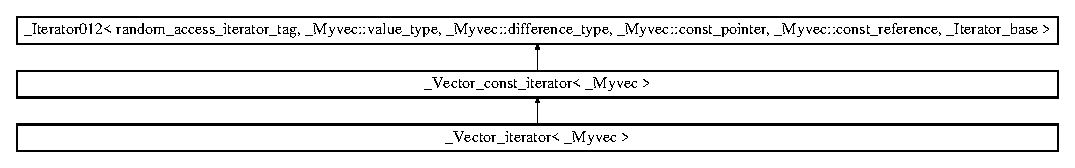
\includegraphics[height=1.814255cm]{class___vector__iterator}
\end{center}
\end{figure}
\subsection*{Public Types}
\begin{DoxyCompactItemize}
\item 
typedef \hyperlink{class___vector__iterator}{\+\_\+\+Vector\+\_\+iterator}$<$ \+\_\+\+Myvec $>$ \hyperlink{class___vector__iterator_a207a91d767f8b7b96d0b375b9dbc8731}{\+\_\+\+Myiter}
\item 
typedef \hyperlink{class___vector__const__iterator}{\+\_\+\+Vector\+\_\+const\+\_\+iterator}\\*
$<$ \+\_\+\+Myvec $>$ \hyperlink{class___vector__iterator_a62a662bae2cce37b78e1b581c15b2d2f}{\+\_\+\+Mybase}
\item 
typedef random\+\_\+access\+\_\+iterator\+\_\+tag \hyperlink{class___vector__iterator_a006e733e2d90ae9efd29706dfa13b852}{iterator\+\_\+category}
\item 
typedef \+\_\+\+Myvec\+::value\+\_\+type \hyperlink{class___vector__iterator_a8b4b40f1be9b179c801618301d4c1ca6}{value\+\_\+type}
\item 
typedef \+\_\+\+Myvec\+::difference\+\_\+type \hyperlink{class___vector__iterator_a2ae251a7a575573a37b141db607a2f3d}{difference\+\_\+type}
\item 
typedef \+\_\+\+Myvec\+::pointer \hyperlink{class___vector__iterator_ab246deee0546c9ff56abdda572e6bfdd}{pointer}
\item 
typedef \+\_\+\+Myvec\+::reference \hyperlink{class___vector__iterator_a854f9738b7e51e509531d5b5c649bf8b}{reference}
\item 
typedef \hyperlink{class___vector__const__iterator_a301a1187c227c820bd86335496229e6a}{pointer} \hyperlink{class___vector__iterator_a9707cfb9b3706ab297a178e6afeaae9b}{\+\_\+\+Unchecked\+\_\+type}
\end{DoxyCompactItemize}
\subsection*{Public Member Functions}
\begin{DoxyCompactItemize}
\item 
\hyperlink{class___vector__iterator_a9fc76d6179a75914582b7200686831bb}{\+\_\+\+Vector\+\_\+iterator} ()
\item 
\hyperlink{class___vector__iterator_a9cd2942135f3dac16a87780426359097}{\+\_\+\+Vector\+\_\+iterator} (\hyperlink{class___vector__const__iterator_a301a1187c227c820bd86335496229e6a}{pointer} \+\_\+\+Parg, const \+\_\+\+Container\+\_\+base $\ast$\+\_\+\+Pvector)
\item 
\hyperlink{class___vector__const__iterator_ac41cce1a95dfa665c2d7237fd94d776b}{\+\_\+\+Myiter} \& \hyperlink{class___vector__iterator_acefd479aa8f5896943bdd945f8acc42f}{\+\_\+\+Rechecked} (\hyperlink{class___vector__const__iterator_a17897ed20e5a6c25f9b383d0f0a4bb9d}{\+\_\+\+Unchecked\+\_\+type} \+\_\+\+Right)
\item 
\hyperlink{class___vector__const__iterator_a17897ed20e5a6c25f9b383d0f0a4bb9d}{\+\_\+\+Unchecked\+\_\+type} \hyperlink{class___vector__iterator_ad65487fdb21c5884dbfac53a8c6ad374}{\+\_\+\+Unchecked} () const 
\item 
\hyperlink{class___vector__const__iterator_ad622d2f855c02a5b3b2f49f39cbbabf4}{reference} \hyperlink{class___vector__iterator_a383ffeb3f02911746695882f9eaf30e7}{operator$\ast$} () const 
\item 
\hyperlink{class___vector__const__iterator_a301a1187c227c820bd86335496229e6a}{pointer} \hyperlink{class___vector__iterator_a96df6099708efb35589933c5daeb0bea}{operator-\/$>$} () const 
\item 
\hyperlink{class___vector__const__iterator_ac41cce1a95dfa665c2d7237fd94d776b}{\+\_\+\+Myiter} \& \hyperlink{class___vector__iterator_a9171d2ff57d806f4468f9cea0eda6ad8}{operator++} ()
\item 
\hyperlink{class___vector__const__iterator_ac41cce1a95dfa665c2d7237fd94d776b}{\+\_\+\+Myiter} \hyperlink{class___vector__iterator_a99fb2657716d84e921cbb984ab594733}{operator++} (int)
\item 
\hyperlink{class___vector__const__iterator_ac41cce1a95dfa665c2d7237fd94d776b}{\+\_\+\+Myiter} \& \hyperlink{class___vector__iterator_ad5103b4825d1b3c2b50273940b3b6613}{operator-\/-\/} ()
\item 
\hyperlink{class___vector__const__iterator_ac41cce1a95dfa665c2d7237fd94d776b}{\+\_\+\+Myiter} \hyperlink{class___vector__iterator_a935b4c4f379d2ea763361857e6bb63ac}{operator-\/-\/} (int)
\item 
\hyperlink{class___vector__const__iterator_ac41cce1a95dfa665c2d7237fd94d776b}{\+\_\+\+Myiter} \& \hyperlink{class___vector__iterator_a52d3b237e619b02430225a4e8553f5ec}{operator+=} (\hyperlink{class___vector__const__iterator_a4fad8668028c0db06eda92c190eeca39}{difference\+\_\+type} \+\_\+\+Off)
\item 
\hyperlink{class___vector__const__iterator_ac41cce1a95dfa665c2d7237fd94d776b}{\+\_\+\+Myiter} \hyperlink{class___vector__iterator_a3f06cc6f1d241585ab5d4d92e4d6409d}{operator+} (\hyperlink{class___vector__const__iterator_a4fad8668028c0db06eda92c190eeca39}{difference\+\_\+type} \+\_\+\+Off) const 
\item 
\hyperlink{class___vector__const__iterator_ac41cce1a95dfa665c2d7237fd94d776b}{\+\_\+\+Myiter} \& \hyperlink{class___vector__iterator_a5e7ba3c086277ff3750077b61390a6c3}{operator-\/=} (\hyperlink{class___vector__const__iterator_a4fad8668028c0db06eda92c190eeca39}{difference\+\_\+type} \+\_\+\+Off)
\item 
\hyperlink{class___vector__const__iterator_ac41cce1a95dfa665c2d7237fd94d776b}{\+\_\+\+Myiter} \hyperlink{class___vector__iterator_a121e9e2805188ce645a77496559120ab}{operator-\/} (\hyperlink{class___vector__const__iterator_a4fad8668028c0db06eda92c190eeca39}{difference\+\_\+type} \+\_\+\+Off) const 
\item 
\hyperlink{class___vector__const__iterator_a4fad8668028c0db06eda92c190eeca39}{difference\+\_\+type} \hyperlink{class___vector__iterator_a02d060bfcfec3049aa6c149428e721d2}{operator-\/} (const \hyperlink{class___vector__iterator_a62a662bae2cce37b78e1b581c15b2d2f}{\+\_\+\+Mybase} \&\+\_\+\+Right) const 
\item 
\hyperlink{class___vector__const__iterator_ad622d2f855c02a5b3b2f49f39cbbabf4}{reference} \hyperlink{class___vector__iterator_a02a084f0f4608220566f34fe4a0ebf94}{operator\mbox{[}$\,$\mbox{]}} (\hyperlink{class___vector__const__iterator_a4fad8668028c0db06eda92c190eeca39}{difference\+\_\+type} \+\_\+\+Off) const 
\end{DoxyCompactItemize}
\subsection*{Additional Inherited Members}


\subsection{Detailed Description}
\subsubsection*{template$<$class \+\_\+\+Myvec$>$class \+\_\+\+Vector\+\_\+iterator$<$ \+\_\+\+Myvec $>$}



Definition at line 285 of file vector.\+h.



\subsection{Member Typedef Documentation}
\hypertarget{class___vector__iterator_a62a662bae2cce37b78e1b581c15b2d2f}{\index{\+\_\+\+Vector\+\_\+iterator@{\+\_\+\+Vector\+\_\+iterator}!\+\_\+\+Mybase@{\+\_\+\+Mybase}}
\index{\+\_\+\+Mybase@{\+\_\+\+Mybase}!\+\_\+\+Vector\+\_\+iterator@{\+\_\+\+Vector\+\_\+iterator}}
\subsubsection[{\+\_\+\+Mybase}]{\setlength{\rightskip}{0pt plus 5cm}template$<$class \+\_\+\+Myvec$>$ typedef {\bf \+\_\+\+Vector\+\_\+const\+\_\+iterator}$<$\+\_\+\+Myvec$>$ {\bf \+\_\+\+Vector\+\_\+iterator}$<$ \+\_\+\+Myvec $>$\+::{\bf \+\_\+\+Mybase}}}\label{class___vector__iterator_a62a662bae2cce37b78e1b581c15b2d2f}


Definition at line 290 of file vector.\+h.

\hypertarget{class___vector__iterator_a207a91d767f8b7b96d0b375b9dbc8731}{\index{\+\_\+\+Vector\+\_\+iterator@{\+\_\+\+Vector\+\_\+iterator}!\+\_\+\+Myiter@{\+\_\+\+Myiter}}
\index{\+\_\+\+Myiter@{\+\_\+\+Myiter}!\+\_\+\+Vector\+\_\+iterator@{\+\_\+\+Vector\+\_\+iterator}}
\subsubsection[{\+\_\+\+Myiter}]{\setlength{\rightskip}{0pt plus 5cm}template$<$class \+\_\+\+Myvec$>$ typedef {\bf \+\_\+\+Vector\+\_\+iterator}$<$\+\_\+\+Myvec$>$ {\bf \+\_\+\+Vector\+\_\+iterator}$<$ \+\_\+\+Myvec $>$\+::{\bf \+\_\+\+Myiter}}}\label{class___vector__iterator_a207a91d767f8b7b96d0b375b9dbc8731}


Definition at line 289 of file vector.\+h.

\hypertarget{class___vector__iterator_a9707cfb9b3706ab297a178e6afeaae9b}{\index{\+\_\+\+Vector\+\_\+iterator@{\+\_\+\+Vector\+\_\+iterator}!\+\_\+\+Unchecked\+\_\+type@{\+\_\+\+Unchecked\+\_\+type}}
\index{\+\_\+\+Unchecked\+\_\+type@{\+\_\+\+Unchecked\+\_\+type}!\+\_\+\+Vector\+\_\+iterator@{\+\_\+\+Vector\+\_\+iterator}}
\subsubsection[{\+\_\+\+Unchecked\+\_\+type}]{\setlength{\rightskip}{0pt plus 5cm}template$<$class \+\_\+\+Myvec$>$ typedef {\bf pointer} {\bf \+\_\+\+Vector\+\_\+iterator}$<$ \+\_\+\+Myvec $>$\+::{\bf \+\_\+\+Unchecked\+\_\+type}}}\label{class___vector__iterator_a9707cfb9b3706ab297a178e6afeaae9b}


Definition at line 307 of file vector.\+h.

\hypertarget{class___vector__iterator_a2ae251a7a575573a37b141db607a2f3d}{\index{\+\_\+\+Vector\+\_\+iterator@{\+\_\+\+Vector\+\_\+iterator}!difference\+\_\+type@{difference\+\_\+type}}
\index{difference\+\_\+type@{difference\+\_\+type}!\+\_\+\+Vector\+\_\+iterator@{\+\_\+\+Vector\+\_\+iterator}}
\subsubsection[{difference\+\_\+type}]{\setlength{\rightskip}{0pt plus 5cm}template$<$class \+\_\+\+Myvec$>$ typedef \+\_\+\+Myvec\+::difference\+\_\+type {\bf \+\_\+\+Vector\+\_\+iterator}$<$ \+\_\+\+Myvec $>$\+::{\bf difference\+\_\+type}}}\label{class___vector__iterator_a2ae251a7a575573a37b141db607a2f3d}


Definition at line 294 of file vector.\+h.

\hypertarget{class___vector__iterator_a006e733e2d90ae9efd29706dfa13b852}{\index{\+\_\+\+Vector\+\_\+iterator@{\+\_\+\+Vector\+\_\+iterator}!iterator\+\_\+category@{iterator\+\_\+category}}
\index{iterator\+\_\+category@{iterator\+\_\+category}!\+\_\+\+Vector\+\_\+iterator@{\+\_\+\+Vector\+\_\+iterator}}
\subsubsection[{iterator\+\_\+category}]{\setlength{\rightskip}{0pt plus 5cm}template$<$class \+\_\+\+Myvec$>$ typedef random\+\_\+access\+\_\+iterator\+\_\+tag {\bf \+\_\+\+Vector\+\_\+iterator}$<$ \+\_\+\+Myvec $>$\+::{\bf iterator\+\_\+category}}}\label{class___vector__iterator_a006e733e2d90ae9efd29706dfa13b852}


Definition at line 291 of file vector.\+h.

\hypertarget{class___vector__iterator_ab246deee0546c9ff56abdda572e6bfdd}{\index{\+\_\+\+Vector\+\_\+iterator@{\+\_\+\+Vector\+\_\+iterator}!pointer@{pointer}}
\index{pointer@{pointer}!\+\_\+\+Vector\+\_\+iterator@{\+\_\+\+Vector\+\_\+iterator}}
\subsubsection[{pointer}]{\setlength{\rightskip}{0pt plus 5cm}template$<$class \+\_\+\+Myvec$>$ typedef \+\_\+\+Myvec\+::pointer {\bf \+\_\+\+Vector\+\_\+iterator}$<$ \+\_\+\+Myvec $>$\+::{\bf pointer}}}\label{class___vector__iterator_ab246deee0546c9ff56abdda572e6bfdd}


Definition at line 295 of file vector.\+h.

\hypertarget{class___vector__iterator_a854f9738b7e51e509531d5b5c649bf8b}{\index{\+\_\+\+Vector\+\_\+iterator@{\+\_\+\+Vector\+\_\+iterator}!reference@{reference}}
\index{reference@{reference}!\+\_\+\+Vector\+\_\+iterator@{\+\_\+\+Vector\+\_\+iterator}}
\subsubsection[{reference}]{\setlength{\rightskip}{0pt plus 5cm}template$<$class \+\_\+\+Myvec$>$ typedef \+\_\+\+Myvec\+::reference {\bf \+\_\+\+Vector\+\_\+iterator}$<$ \+\_\+\+Myvec $>$\+::{\bf reference}}}\label{class___vector__iterator_a854f9738b7e51e509531d5b5c649bf8b}


Definition at line 296 of file vector.\+h.

\hypertarget{class___vector__iterator_a8b4b40f1be9b179c801618301d4c1ca6}{\index{\+\_\+\+Vector\+\_\+iterator@{\+\_\+\+Vector\+\_\+iterator}!value\+\_\+type@{value\+\_\+type}}
\index{value\+\_\+type@{value\+\_\+type}!\+\_\+\+Vector\+\_\+iterator@{\+\_\+\+Vector\+\_\+iterator}}
\subsubsection[{value\+\_\+type}]{\setlength{\rightskip}{0pt plus 5cm}template$<$class \+\_\+\+Myvec$>$ typedef \+\_\+\+Myvec\+::value\+\_\+type {\bf \+\_\+\+Vector\+\_\+iterator}$<$ \+\_\+\+Myvec $>$\+::{\bf value\+\_\+type}}}\label{class___vector__iterator_a8b4b40f1be9b179c801618301d4c1ca6}


Definition at line 293 of file vector.\+h.



\subsection{Constructor \& Destructor Documentation}
\hypertarget{class___vector__iterator_a9fc76d6179a75914582b7200686831bb}{\index{\+\_\+\+Vector\+\_\+iterator@{\+\_\+\+Vector\+\_\+iterator}!\+\_\+\+Vector\+\_\+iterator@{\+\_\+\+Vector\+\_\+iterator}}
\index{\+\_\+\+Vector\+\_\+iterator@{\+\_\+\+Vector\+\_\+iterator}!\+\_\+\+Vector\+\_\+iterator@{\+\_\+\+Vector\+\_\+iterator}}
\subsubsection[{\+\_\+\+Vector\+\_\+iterator}]{\setlength{\rightskip}{0pt plus 5cm}template$<$class \+\_\+\+Myvec$>$ {\bf \+\_\+\+Vector\+\_\+iterator}$<$ \+\_\+\+Myvec $>$\+::{\bf \+\_\+\+Vector\+\_\+iterator} (
\begin{DoxyParamCaption}
{}
\end{DoxyParamCaption}
)\hspace{0.3cm}{\ttfamily [inline]}}}\label{class___vector__iterator_a9fc76d6179a75914582b7200686831bb}


Definition at line 298 of file vector.\+h.

\hypertarget{class___vector__iterator_a9cd2942135f3dac16a87780426359097}{\index{\+\_\+\+Vector\+\_\+iterator@{\+\_\+\+Vector\+\_\+iterator}!\+\_\+\+Vector\+\_\+iterator@{\+\_\+\+Vector\+\_\+iterator}}
\index{\+\_\+\+Vector\+\_\+iterator@{\+\_\+\+Vector\+\_\+iterator}!\+\_\+\+Vector\+\_\+iterator@{\+\_\+\+Vector\+\_\+iterator}}
\subsubsection[{\+\_\+\+Vector\+\_\+iterator}]{\setlength{\rightskip}{0pt plus 5cm}template$<$class \+\_\+\+Myvec$>$ {\bf \+\_\+\+Vector\+\_\+iterator}$<$ \+\_\+\+Myvec $>$\+::{\bf \+\_\+\+Vector\+\_\+iterator} (
\begin{DoxyParamCaption}
\item[{{\bf pointer}}]{\+\_\+\+Parg, }
\item[{const \+\_\+\+Container\+\_\+base $\ast$}]{\+\_\+\+Pvector}
\end{DoxyParamCaption}
)\hspace{0.3cm}{\ttfamily [inline]}}}\label{class___vector__iterator_a9cd2942135f3dac16a87780426359097}


Definition at line 302 of file vector.\+h.



\subsection{Member Function Documentation}
\hypertarget{class___vector__iterator_acefd479aa8f5896943bdd945f8acc42f}{\index{\+\_\+\+Vector\+\_\+iterator@{\+\_\+\+Vector\+\_\+iterator}!\+\_\+\+Rechecked@{\+\_\+\+Rechecked}}
\index{\+\_\+\+Rechecked@{\+\_\+\+Rechecked}!\+\_\+\+Vector\+\_\+iterator@{\+\_\+\+Vector\+\_\+iterator}}
\subsubsection[{\+\_\+\+Rechecked}]{\setlength{\rightskip}{0pt plus 5cm}template$<$class \+\_\+\+Myvec$>$ {\bf \+\_\+\+Myiter}\& {\bf \+\_\+\+Vector\+\_\+iterator}$<$ \+\_\+\+Myvec $>$\+::\+\_\+\+Rechecked (
\begin{DoxyParamCaption}
\item[{{\bf \+\_\+\+Unchecked\+\_\+type}}]{\+\_\+\+Right}
\end{DoxyParamCaption}
)\hspace{0.3cm}{\ttfamily [inline]}}}\label{class___vector__iterator_acefd479aa8f5896943bdd945f8acc42f}


Definition at line 309 of file vector.\+h.

\hypertarget{class___vector__iterator_ad65487fdb21c5884dbfac53a8c6ad374}{\index{\+\_\+\+Vector\+\_\+iterator@{\+\_\+\+Vector\+\_\+iterator}!\+\_\+\+Unchecked@{\+\_\+\+Unchecked}}
\index{\+\_\+\+Unchecked@{\+\_\+\+Unchecked}!\+\_\+\+Vector\+\_\+iterator@{\+\_\+\+Vector\+\_\+iterator}}
\subsubsection[{\+\_\+\+Unchecked}]{\setlength{\rightskip}{0pt plus 5cm}template$<$class \+\_\+\+Myvec$>$ {\bf \+\_\+\+Unchecked\+\_\+type} {\bf \+\_\+\+Vector\+\_\+iterator}$<$ \+\_\+\+Myvec $>$\+::\+\_\+\+Unchecked (
\begin{DoxyParamCaption}
{}
\end{DoxyParamCaption}
) const\hspace{0.3cm}{\ttfamily [inline]}}}\label{class___vector__iterator_ad65487fdb21c5884dbfac53a8c6ad374}


Definition at line 315 of file vector.\+h.

\hypertarget{class___vector__iterator_a383ffeb3f02911746695882f9eaf30e7}{\index{\+\_\+\+Vector\+\_\+iterator@{\+\_\+\+Vector\+\_\+iterator}!operator$\ast$@{operator$\ast$}}
\index{operator$\ast$@{operator$\ast$}!\+\_\+\+Vector\+\_\+iterator@{\+\_\+\+Vector\+\_\+iterator}}
\subsubsection[{operator$\ast$}]{\setlength{\rightskip}{0pt plus 5cm}template$<$class \+\_\+\+Myvec$>$ {\bf reference} {\bf \+\_\+\+Vector\+\_\+iterator}$<$ \+\_\+\+Myvec $>$\+::operator$\ast$ (
\begin{DoxyParamCaption}
{}
\end{DoxyParamCaption}
) const\hspace{0.3cm}{\ttfamily [inline]}}}\label{class___vector__iterator_a383ffeb3f02911746695882f9eaf30e7}


Definition at line 320 of file vector.\+h.

\hypertarget{class___vector__iterator_a3f06cc6f1d241585ab5d4d92e4d6409d}{\index{\+\_\+\+Vector\+\_\+iterator@{\+\_\+\+Vector\+\_\+iterator}!operator+@{operator+}}
\index{operator+@{operator+}!\+\_\+\+Vector\+\_\+iterator@{\+\_\+\+Vector\+\_\+iterator}}
\subsubsection[{operator+}]{\setlength{\rightskip}{0pt plus 5cm}template$<$class \+\_\+\+Myvec$>$ {\bf \+\_\+\+Myiter} {\bf \+\_\+\+Vector\+\_\+iterator}$<$ \+\_\+\+Myvec $>$\+::operator+ (
\begin{DoxyParamCaption}
\item[{{\bf difference\+\_\+type}}]{\+\_\+\+Off}
\end{DoxyParamCaption}
) const\hspace{0.3cm}{\ttfamily [inline]}}}\label{class___vector__iterator_a3f06cc6f1d241585ab5d4d92e4d6409d}


Definition at line 362 of file vector.\+h.

\hypertarget{class___vector__iterator_a9171d2ff57d806f4468f9cea0eda6ad8}{\index{\+\_\+\+Vector\+\_\+iterator@{\+\_\+\+Vector\+\_\+iterator}!operator++@{operator++}}
\index{operator++@{operator++}!\+\_\+\+Vector\+\_\+iterator@{\+\_\+\+Vector\+\_\+iterator}}
\subsubsection[{operator++}]{\setlength{\rightskip}{0pt plus 5cm}template$<$class \+\_\+\+Myvec$>$ {\bf \+\_\+\+Myiter}\& {\bf \+\_\+\+Vector\+\_\+iterator}$<$ \+\_\+\+Myvec $>$\+::operator++ (
\begin{DoxyParamCaption}
{}
\end{DoxyParamCaption}
)\hspace{0.3cm}{\ttfamily [inline]}}}\label{class___vector__iterator_a9171d2ff57d806f4468f9cea0eda6ad8}


Definition at line 330 of file vector.\+h.

\hypertarget{class___vector__iterator_a99fb2657716d84e921cbb984ab594733}{\index{\+\_\+\+Vector\+\_\+iterator@{\+\_\+\+Vector\+\_\+iterator}!operator++@{operator++}}
\index{operator++@{operator++}!\+\_\+\+Vector\+\_\+iterator@{\+\_\+\+Vector\+\_\+iterator}}
\subsubsection[{operator++}]{\setlength{\rightskip}{0pt plus 5cm}template$<$class \+\_\+\+Myvec$>$ {\bf \+\_\+\+Myiter} {\bf \+\_\+\+Vector\+\_\+iterator}$<$ \+\_\+\+Myvec $>$\+::operator++ (
\begin{DoxyParamCaption}
\item[{int}]{}
\end{DoxyParamCaption}
)\hspace{0.3cm}{\ttfamily [inline]}}}\label{class___vector__iterator_a99fb2657716d84e921cbb984ab594733}


Definition at line 336 of file vector.\+h.

\hypertarget{class___vector__iterator_a52d3b237e619b02430225a4e8553f5ec}{\index{\+\_\+\+Vector\+\_\+iterator@{\+\_\+\+Vector\+\_\+iterator}!operator+=@{operator+=}}
\index{operator+=@{operator+=}!\+\_\+\+Vector\+\_\+iterator@{\+\_\+\+Vector\+\_\+iterator}}
\subsubsection[{operator+=}]{\setlength{\rightskip}{0pt plus 5cm}template$<$class \+\_\+\+Myvec$>$ {\bf \+\_\+\+Myiter}\& {\bf \+\_\+\+Vector\+\_\+iterator}$<$ \+\_\+\+Myvec $>$\+::operator+= (
\begin{DoxyParamCaption}
\item[{{\bf difference\+\_\+type}}]{\+\_\+\+Off}
\end{DoxyParamCaption}
)\hspace{0.3cm}{\ttfamily [inline]}}}\label{class___vector__iterator_a52d3b237e619b02430225a4e8553f5ec}


Definition at line 356 of file vector.\+h.

\hypertarget{class___vector__iterator_a121e9e2805188ce645a77496559120ab}{\index{\+\_\+\+Vector\+\_\+iterator@{\+\_\+\+Vector\+\_\+iterator}!operator-\/@{operator-\/}}
\index{operator-\/@{operator-\/}!\+\_\+\+Vector\+\_\+iterator@{\+\_\+\+Vector\+\_\+iterator}}
\subsubsection[{operator-\/}]{\setlength{\rightskip}{0pt plus 5cm}template$<$class \+\_\+\+Myvec$>$ {\bf \+\_\+\+Myiter} {\bf \+\_\+\+Vector\+\_\+iterator}$<$ \+\_\+\+Myvec $>$\+::operator-\/ (
\begin{DoxyParamCaption}
\item[{{\bf difference\+\_\+type}}]{\+\_\+\+Off}
\end{DoxyParamCaption}
) const\hspace{0.3cm}{\ttfamily [inline]}}}\label{class___vector__iterator_a121e9e2805188ce645a77496559120ab}


Definition at line 373 of file vector.\+h.

\hypertarget{class___vector__iterator_a02d060bfcfec3049aa6c149428e721d2}{\index{\+\_\+\+Vector\+\_\+iterator@{\+\_\+\+Vector\+\_\+iterator}!operator-\/@{operator-\/}}
\index{operator-\/@{operator-\/}!\+\_\+\+Vector\+\_\+iterator@{\+\_\+\+Vector\+\_\+iterator}}
\subsubsection[{operator-\/}]{\setlength{\rightskip}{0pt plus 5cm}template$<$class \+\_\+\+Myvec$>$ {\bf difference\+\_\+type} {\bf \+\_\+\+Vector\+\_\+iterator}$<$ \+\_\+\+Myvec $>$\+::operator-\/ (
\begin{DoxyParamCaption}
\item[{const {\bf \+\_\+\+Mybase} \&}]{\+\_\+\+Right}
\end{DoxyParamCaption}
) const\hspace{0.3cm}{\ttfamily [inline]}}}\label{class___vector__iterator_a02d060bfcfec3049aa6c149428e721d2}


Definition at line 379 of file vector.\+h.

\hypertarget{class___vector__iterator_ad5103b4825d1b3c2b50273940b3b6613}{\index{\+\_\+\+Vector\+\_\+iterator@{\+\_\+\+Vector\+\_\+iterator}!operator-\/-\/@{operator-\/-\/}}
\index{operator-\/-\/@{operator-\/-\/}!\+\_\+\+Vector\+\_\+iterator@{\+\_\+\+Vector\+\_\+iterator}}
\subsubsection[{operator-\/-\/}]{\setlength{\rightskip}{0pt plus 5cm}template$<$class \+\_\+\+Myvec$>$ {\bf \+\_\+\+Myiter}\& {\bf \+\_\+\+Vector\+\_\+iterator}$<$ \+\_\+\+Myvec $>$\+::operator-\/-\/ (
\begin{DoxyParamCaption}
{}
\end{DoxyParamCaption}
)\hspace{0.3cm}{\ttfamily [inline]}}}\label{class___vector__iterator_ad5103b4825d1b3c2b50273940b3b6613}


Definition at line 343 of file vector.\+h.

\hypertarget{class___vector__iterator_a935b4c4f379d2ea763361857e6bb63ac}{\index{\+\_\+\+Vector\+\_\+iterator@{\+\_\+\+Vector\+\_\+iterator}!operator-\/-\/@{operator-\/-\/}}
\index{operator-\/-\/@{operator-\/-\/}!\+\_\+\+Vector\+\_\+iterator@{\+\_\+\+Vector\+\_\+iterator}}
\subsubsection[{operator-\/-\/}]{\setlength{\rightskip}{0pt plus 5cm}template$<$class \+\_\+\+Myvec$>$ {\bf \+\_\+\+Myiter} {\bf \+\_\+\+Vector\+\_\+iterator}$<$ \+\_\+\+Myvec $>$\+::operator-\/-\/ (
\begin{DoxyParamCaption}
\item[{int}]{}
\end{DoxyParamCaption}
)\hspace{0.3cm}{\ttfamily [inline]}}}\label{class___vector__iterator_a935b4c4f379d2ea763361857e6bb63ac}


Definition at line 349 of file vector.\+h.

\hypertarget{class___vector__iterator_a5e7ba3c086277ff3750077b61390a6c3}{\index{\+\_\+\+Vector\+\_\+iterator@{\+\_\+\+Vector\+\_\+iterator}!operator-\/=@{operator-\/=}}
\index{operator-\/=@{operator-\/=}!\+\_\+\+Vector\+\_\+iterator@{\+\_\+\+Vector\+\_\+iterator}}
\subsubsection[{operator-\/=}]{\setlength{\rightskip}{0pt plus 5cm}template$<$class \+\_\+\+Myvec$>$ {\bf \+\_\+\+Myiter}\& {\bf \+\_\+\+Vector\+\_\+iterator}$<$ \+\_\+\+Myvec $>$\+::operator-\/= (
\begin{DoxyParamCaption}
\item[{{\bf difference\+\_\+type}}]{\+\_\+\+Off}
\end{DoxyParamCaption}
)\hspace{0.3cm}{\ttfamily [inline]}}}\label{class___vector__iterator_a5e7ba3c086277ff3750077b61390a6c3}


Definition at line 368 of file vector.\+h.

\hypertarget{class___vector__iterator_a96df6099708efb35589933c5daeb0bea}{\index{\+\_\+\+Vector\+\_\+iterator@{\+\_\+\+Vector\+\_\+iterator}!operator-\/$>$@{operator-\/$>$}}
\index{operator-\/$>$@{operator-\/$>$}!\+\_\+\+Vector\+\_\+iterator@{\+\_\+\+Vector\+\_\+iterator}}
\subsubsection[{operator-\/$>$}]{\setlength{\rightskip}{0pt plus 5cm}template$<$class \+\_\+\+Myvec$>$ {\bf pointer} {\bf \+\_\+\+Vector\+\_\+iterator}$<$ \+\_\+\+Myvec $>$\+::operator-\/$>$ (
\begin{DoxyParamCaption}
{}
\end{DoxyParamCaption}
) const\hspace{0.3cm}{\ttfamily [inline]}}}\label{class___vector__iterator_a96df6099708efb35589933c5daeb0bea}


Definition at line 325 of file vector.\+h.

\hypertarget{class___vector__iterator_a02a084f0f4608220566f34fe4a0ebf94}{\index{\+\_\+\+Vector\+\_\+iterator@{\+\_\+\+Vector\+\_\+iterator}!operator\mbox{[}$\,$\mbox{]}@{operator[]}}
\index{operator\mbox{[}$\,$\mbox{]}@{operator[]}!\+\_\+\+Vector\+\_\+iterator@{\+\_\+\+Vector\+\_\+iterator}}
\subsubsection[{operator[]}]{\setlength{\rightskip}{0pt plus 5cm}template$<$class \+\_\+\+Myvec$>$ {\bf reference} {\bf \+\_\+\+Vector\+\_\+iterator}$<$ \+\_\+\+Myvec $>$\+::operator\mbox{[}$\,$\mbox{]} (
\begin{DoxyParamCaption}
\item[{{\bf difference\+\_\+type}}]{\+\_\+\+Off}
\end{DoxyParamCaption}
) const\hspace{0.3cm}{\ttfamily [inline]}}}\label{class___vector__iterator_a02a084f0f4608220566f34fe4a0ebf94}


Definition at line 384 of file vector.\+h.



The documentation for this class was generated from the following file\+:\begin{DoxyCompactItemize}
\item 
\hyperlink{vector_8h}{vector.\+h}\end{DoxyCompactItemize}

\hypertarget{class___vector__val}{\section{\+\_\+\+Vector\+\_\+val$<$ \+\_\+\+Ty, \+\_\+\+Alloc $>$ Class Template Reference}
\label{class___vector__val}\index{\+\_\+\+Vector\+\_\+val$<$ \+\_\+\+Ty, \+\_\+\+Alloc $>$@{\+\_\+\+Vector\+\_\+val$<$ \+\_\+\+Ty, \+\_\+\+Alloc $>$}}
}


{\ttfamily \#include $<$vector.\+h$>$}

Inheritance diagram for \+\_\+\+Vector\+\_\+val$<$ \+\_\+\+Ty, \+\_\+\+Alloc $>$\+:\begin{figure}[H]
\begin{center}
\leavevmode
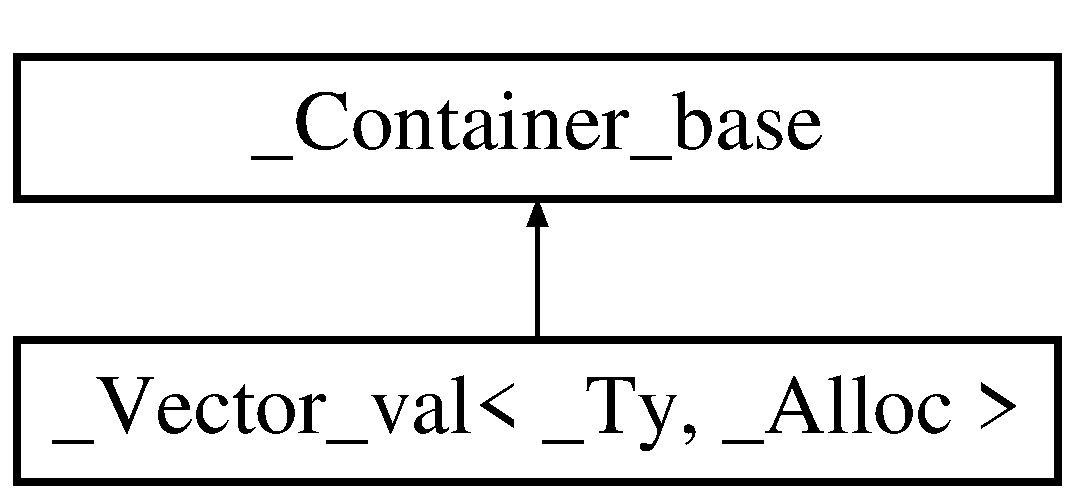
\includegraphics[height=2.000000cm]{class___vector__val}
\end{center}
\end{figure}
\subsection*{Public Types}
\begin{DoxyCompactItemize}
\item 
typedef \+\_\+\+Alloc\+::template \\*
rebind$<$ \+\_\+\+Ty $>$\+::other \hyperlink{class___vector__val_ad273d1146bf265f65e75133aa2f9986a}{\+\_\+\+Alty}
\item 
typedef \+\_\+\+Alty\+::size\+\_\+type \hyperlink{class___vector__val_a46109be8e2eefdf86304a44e05074941}{size\+\_\+type}
\item 
typedef \+\_\+\+Alty\+::difference\+\_\+type \hyperlink{class___vector__val_ac80d6a645f27bc921bf30f5b0acdffb4}{difference\+\_\+type}
\item 
typedef \+\_\+\+Alty\+::pointer \hyperlink{class___vector__val_ae6cca5a50b243bc20bd27fa8f620d63e}{pointer}
\item 
typedef \+\_\+\+Alty\+::const\+\_\+pointer \hyperlink{class___vector__val_ab8b3d3a2093e4799ac46bf479e8789bb}{const\+\_\+pointer}
\item 
typedef \+\_\+\+Alty\+::reference \hyperlink{class___vector__val_a87f4bfea49b67e864cba8029a999eefe}{reference}
\item 
typedef \+\_\+\+Alty\+::const\+\_\+reference \hyperlink{class___vector__val_a0c18884755addbb2c0530338682d3506}{const\+\_\+reference}
\item 
typedef \+\_\+\+Alty\+::value\+\_\+type \hyperlink{class___vector__val_ad185b733a2aa2cd3df73e23303d5c43e}{value\+\_\+type}
\end{DoxyCompactItemize}
\subsection*{Public Member Functions}
\begin{DoxyCompactItemize}
\item 
\hyperlink{class___vector__val_a06a11b0429e308118aaa63bda49040f1}{\+\_\+\+Vector\+\_\+val} (\+\_\+\+Alloc \+\_\+\+Al=\+\_\+\+Alloc())
\item 
\hyperlink{class___vector__val_a2e7cc72fb5c7241f0015e7ec4ace117d}{$\sim$\+\_\+\+Vector\+\_\+val} ()
\end{DoxyCompactItemize}
\subsection*{Public Attributes}
\begin{DoxyCompactItemize}
\item 
\hyperlink{class___vector__val_ae6cca5a50b243bc20bd27fa8f620d63e}{pointer} \hyperlink{class___vector__val_ac10d5b268d1c2c005f2b9257e5458ec7}{\+\_\+\+Myfirst}
\item 
\hyperlink{class___vector__val_ae6cca5a50b243bc20bd27fa8f620d63e}{pointer} \hyperlink{class___vector__val_a76c098026a887586c12c91249908ecd9}{\+\_\+\+Mylast}
\item 
\hyperlink{class___vector__val_ae6cca5a50b243bc20bd27fa8f620d63e}{pointer} \hyperlink{class___vector__val_a6ae5d0e49562c6cc6b697450284cda58}{\+\_\+\+Myend}
\item 
\hyperlink{class___vector__val_ad273d1146bf265f65e75133aa2f9986a}{\+\_\+\+Alty} \hyperlink{class___vector__val_a86df8093d4b6a58caa7e8d7ff0c441fd}{\+\_\+\+Alval}
\end{DoxyCompactItemize}


\subsection{Detailed Description}
\subsubsection*{template$<$class \+\_\+\+Ty, class \+\_\+\+Alloc$>$class \+\_\+\+Vector\+\_\+val$<$ \+\_\+\+Ty, \+\_\+\+Alloc $>$}



Definition at line 417 of file vector.\+h.



\subsection{Member Typedef Documentation}
\hypertarget{class___vector__val_ad273d1146bf265f65e75133aa2f9986a}{\index{\+\_\+\+Vector\+\_\+val@{\+\_\+\+Vector\+\_\+val}!\+\_\+\+Alty@{\+\_\+\+Alty}}
\index{\+\_\+\+Alty@{\+\_\+\+Alty}!\+\_\+\+Vector\+\_\+val@{\+\_\+\+Vector\+\_\+val}}
\subsubsection[{\+\_\+\+Alty}]{\setlength{\rightskip}{0pt plus 5cm}template$<$class \+\_\+\+Ty, class \+\_\+\+Alloc$>$ typedef \+\_\+\+Alloc\+::template rebind$<$\+\_\+\+Ty$>$\+::other {\bf \+\_\+\+Vector\+\_\+val}$<$ \+\_\+\+Ty, \+\_\+\+Alloc $>$\+::{\bf \+\_\+\+Alty}}}\label{class___vector__val_ad273d1146bf265f65e75133aa2f9986a}


Definition at line 421 of file vector.\+h.

\hypertarget{class___vector__val_ab8b3d3a2093e4799ac46bf479e8789bb}{\index{\+\_\+\+Vector\+\_\+val@{\+\_\+\+Vector\+\_\+val}!const\+\_\+pointer@{const\+\_\+pointer}}
\index{const\+\_\+pointer@{const\+\_\+pointer}!\+\_\+\+Vector\+\_\+val@{\+\_\+\+Vector\+\_\+val}}
\subsubsection[{const\+\_\+pointer}]{\setlength{\rightskip}{0pt plus 5cm}template$<$class \+\_\+\+Ty, class \+\_\+\+Alloc$>$ typedef \+\_\+\+Alty\+::const\+\_\+pointer {\bf \+\_\+\+Vector\+\_\+val}$<$ \+\_\+\+Ty, \+\_\+\+Alloc $>$\+::{\bf const\+\_\+pointer}}}\label{class___vector__val_ab8b3d3a2093e4799ac46bf479e8789bb}


Definition at line 465 of file vector.\+h.

\hypertarget{class___vector__val_a0c18884755addbb2c0530338682d3506}{\index{\+\_\+\+Vector\+\_\+val@{\+\_\+\+Vector\+\_\+val}!const\+\_\+reference@{const\+\_\+reference}}
\index{const\+\_\+reference@{const\+\_\+reference}!\+\_\+\+Vector\+\_\+val@{\+\_\+\+Vector\+\_\+val}}
\subsubsection[{const\+\_\+reference}]{\setlength{\rightskip}{0pt plus 5cm}template$<$class \+\_\+\+Ty, class \+\_\+\+Alloc$>$ typedef \+\_\+\+Alty\+::const\+\_\+reference {\bf \+\_\+\+Vector\+\_\+val}$<$ \+\_\+\+Ty, \+\_\+\+Alloc $>$\+::{\bf const\+\_\+reference}}}\label{class___vector__val_a0c18884755addbb2c0530338682d3506}


Definition at line 467 of file vector.\+h.

\hypertarget{class___vector__val_ac80d6a645f27bc921bf30f5b0acdffb4}{\index{\+\_\+\+Vector\+\_\+val@{\+\_\+\+Vector\+\_\+val}!difference\+\_\+type@{difference\+\_\+type}}
\index{difference\+\_\+type@{difference\+\_\+type}!\+\_\+\+Vector\+\_\+val@{\+\_\+\+Vector\+\_\+val}}
\subsubsection[{difference\+\_\+type}]{\setlength{\rightskip}{0pt plus 5cm}template$<$class \+\_\+\+Ty, class \+\_\+\+Alloc$>$ typedef \+\_\+\+Alty\+::difference\+\_\+type {\bf \+\_\+\+Vector\+\_\+val}$<$ \+\_\+\+Ty, \+\_\+\+Alloc $>$\+::{\bf difference\+\_\+type}}}\label{class___vector__val_ac80d6a645f27bc921bf30f5b0acdffb4}


Definition at line 463 of file vector.\+h.

\hypertarget{class___vector__val_ae6cca5a50b243bc20bd27fa8f620d63e}{\index{\+\_\+\+Vector\+\_\+val@{\+\_\+\+Vector\+\_\+val}!pointer@{pointer}}
\index{pointer@{pointer}!\+\_\+\+Vector\+\_\+val@{\+\_\+\+Vector\+\_\+val}}
\subsubsection[{pointer}]{\setlength{\rightskip}{0pt plus 5cm}template$<$class \+\_\+\+Ty, class \+\_\+\+Alloc$>$ typedef \+\_\+\+Alty\+::pointer {\bf \+\_\+\+Vector\+\_\+val}$<$ \+\_\+\+Ty, \+\_\+\+Alloc $>$\+::{\bf pointer}}}\label{class___vector__val_ae6cca5a50b243bc20bd27fa8f620d63e}


Definition at line 464 of file vector.\+h.

\hypertarget{class___vector__val_a87f4bfea49b67e864cba8029a999eefe}{\index{\+\_\+\+Vector\+\_\+val@{\+\_\+\+Vector\+\_\+val}!reference@{reference}}
\index{reference@{reference}!\+\_\+\+Vector\+\_\+val@{\+\_\+\+Vector\+\_\+val}}
\subsubsection[{reference}]{\setlength{\rightskip}{0pt plus 5cm}template$<$class \+\_\+\+Ty, class \+\_\+\+Alloc$>$ typedef \+\_\+\+Alty\+::reference {\bf \+\_\+\+Vector\+\_\+val}$<$ \+\_\+\+Ty, \+\_\+\+Alloc $>$\+::{\bf reference}}}\label{class___vector__val_a87f4bfea49b67e864cba8029a999eefe}


Definition at line 466 of file vector.\+h.

\hypertarget{class___vector__val_a46109be8e2eefdf86304a44e05074941}{\index{\+\_\+\+Vector\+\_\+val@{\+\_\+\+Vector\+\_\+val}!size\+\_\+type@{size\+\_\+type}}
\index{size\+\_\+type@{size\+\_\+type}!\+\_\+\+Vector\+\_\+val@{\+\_\+\+Vector\+\_\+val}}
\subsubsection[{size\+\_\+type}]{\setlength{\rightskip}{0pt plus 5cm}template$<$class \+\_\+\+Ty, class \+\_\+\+Alloc$>$ typedef \+\_\+\+Alty\+::size\+\_\+type {\bf \+\_\+\+Vector\+\_\+val}$<$ \+\_\+\+Ty, \+\_\+\+Alloc $>$\+::{\bf size\+\_\+type}}}\label{class___vector__val_a46109be8e2eefdf86304a44e05074941}


Definition at line 462 of file vector.\+h.

\hypertarget{class___vector__val_ad185b733a2aa2cd3df73e23303d5c43e}{\index{\+\_\+\+Vector\+\_\+val@{\+\_\+\+Vector\+\_\+val}!value\+\_\+type@{value\+\_\+type}}
\index{value\+\_\+type@{value\+\_\+type}!\+\_\+\+Vector\+\_\+val@{\+\_\+\+Vector\+\_\+val}}
\subsubsection[{value\+\_\+type}]{\setlength{\rightskip}{0pt plus 5cm}template$<$class \+\_\+\+Ty, class \+\_\+\+Alloc$>$ typedef \+\_\+\+Alty\+::value\+\_\+type {\bf \+\_\+\+Vector\+\_\+val}$<$ \+\_\+\+Ty, \+\_\+\+Alloc $>$\+::{\bf value\+\_\+type}}}\label{class___vector__val_ad185b733a2aa2cd3df73e23303d5c43e}


Definition at line 468 of file vector.\+h.



\subsection{Constructor \& Destructor Documentation}
\hypertarget{class___vector__val_a06a11b0429e308118aaa63bda49040f1}{\index{\+\_\+\+Vector\+\_\+val@{\+\_\+\+Vector\+\_\+val}!\+\_\+\+Vector\+\_\+val@{\+\_\+\+Vector\+\_\+val}}
\index{\+\_\+\+Vector\+\_\+val@{\+\_\+\+Vector\+\_\+val}!\+\_\+\+Vector\+\_\+val@{\+\_\+\+Vector\+\_\+val}}
\subsubsection[{\+\_\+\+Vector\+\_\+val}]{\setlength{\rightskip}{0pt plus 5cm}template$<$class \+\_\+\+Ty, class \+\_\+\+Alloc$>$ {\bf \+\_\+\+Vector\+\_\+val}$<$ \+\_\+\+Ty, \+\_\+\+Alloc $>$\+::{\bf \+\_\+\+Vector\+\_\+val} (
\begin{DoxyParamCaption}
\item[{\+\_\+\+Alloc}]{\+\_\+\+Al = {\ttfamily \+\_\+Alloc()}}
\end{DoxyParamCaption}
)\hspace{0.3cm}{\ttfamily [inline]}}}\label{class___vector__val_a06a11b0429e308118aaa63bda49040f1}


Definition at line 424 of file vector.\+h.

\hypertarget{class___vector__val_a2e7cc72fb5c7241f0015e7ec4ace117d}{\index{\+\_\+\+Vector\+\_\+val@{\+\_\+\+Vector\+\_\+val}!````~\+\_\+\+Vector\+\_\+val@{$\sim$\+\_\+\+Vector\+\_\+val}}
\index{````~\+\_\+\+Vector\+\_\+val@{$\sim$\+\_\+\+Vector\+\_\+val}!\+\_\+\+Vector\+\_\+val@{\+\_\+\+Vector\+\_\+val}}
\subsubsection[{$\sim$\+\_\+\+Vector\+\_\+val}]{\setlength{\rightskip}{0pt plus 5cm}template$<$class \+\_\+\+Ty, class \+\_\+\+Alloc$>$ {\bf \+\_\+\+Vector\+\_\+val}$<$ \+\_\+\+Ty, \+\_\+\+Alloc $>$\+::$\sim${\bf \+\_\+\+Vector\+\_\+val} (
\begin{DoxyParamCaption}
{}
\end{DoxyParamCaption}
)\hspace{0.3cm}{\ttfamily [inline]}}}\label{class___vector__val_a2e7cc72fb5c7241f0015e7ec4ace117d}


Definition at line 432 of file vector.\+h.



\subsection{Member Data Documentation}
\hypertarget{class___vector__val_a86df8093d4b6a58caa7e8d7ff0c441fd}{\index{\+\_\+\+Vector\+\_\+val@{\+\_\+\+Vector\+\_\+val}!\+\_\+\+Alval@{\+\_\+\+Alval}}
\index{\+\_\+\+Alval@{\+\_\+\+Alval}!\+\_\+\+Vector\+\_\+val@{\+\_\+\+Vector\+\_\+val}}
\subsubsection[{\+\_\+\+Alval}]{\setlength{\rightskip}{0pt plus 5cm}template$<$class \+\_\+\+Ty, class \+\_\+\+Alloc$>$ {\bf \+\_\+\+Alty} {\bf \+\_\+\+Vector\+\_\+val}$<$ \+\_\+\+Ty, \+\_\+\+Alloc $>$\+::\+\_\+\+Alval}}\label{class___vector__val_a86df8093d4b6a58caa7e8d7ff0c441fd}


Definition at line 473 of file vector.\+h.

\hypertarget{class___vector__val_a6ae5d0e49562c6cc6b697450284cda58}{\index{\+\_\+\+Vector\+\_\+val@{\+\_\+\+Vector\+\_\+val}!\+\_\+\+Myend@{\+\_\+\+Myend}}
\index{\+\_\+\+Myend@{\+\_\+\+Myend}!\+\_\+\+Vector\+\_\+val@{\+\_\+\+Vector\+\_\+val}}
\subsubsection[{\+\_\+\+Myend}]{\setlength{\rightskip}{0pt plus 5cm}template$<$class \+\_\+\+Ty, class \+\_\+\+Alloc$>$ {\bf pointer} {\bf \+\_\+\+Vector\+\_\+val}$<$ \+\_\+\+Ty, \+\_\+\+Alloc $>$\+::\+\_\+\+Myend}}\label{class___vector__val_a6ae5d0e49562c6cc6b697450284cda58}


Definition at line 472 of file vector.\+h.

\hypertarget{class___vector__val_ac10d5b268d1c2c005f2b9257e5458ec7}{\index{\+\_\+\+Vector\+\_\+val@{\+\_\+\+Vector\+\_\+val}!\+\_\+\+Myfirst@{\+\_\+\+Myfirst}}
\index{\+\_\+\+Myfirst@{\+\_\+\+Myfirst}!\+\_\+\+Vector\+\_\+val@{\+\_\+\+Vector\+\_\+val}}
\subsubsection[{\+\_\+\+Myfirst}]{\setlength{\rightskip}{0pt plus 5cm}template$<$class \+\_\+\+Ty, class \+\_\+\+Alloc$>$ {\bf pointer} {\bf \+\_\+\+Vector\+\_\+val}$<$ \+\_\+\+Ty, \+\_\+\+Alloc $>$\+::\+\_\+\+Myfirst}}\label{class___vector__val_ac10d5b268d1c2c005f2b9257e5458ec7}


Definition at line 470 of file vector.\+h.

\hypertarget{class___vector__val_a76c098026a887586c12c91249908ecd9}{\index{\+\_\+\+Vector\+\_\+val@{\+\_\+\+Vector\+\_\+val}!\+\_\+\+Mylast@{\+\_\+\+Mylast}}
\index{\+\_\+\+Mylast@{\+\_\+\+Mylast}!\+\_\+\+Vector\+\_\+val@{\+\_\+\+Vector\+\_\+val}}
\subsubsection[{\+\_\+\+Mylast}]{\setlength{\rightskip}{0pt plus 5cm}template$<$class \+\_\+\+Ty, class \+\_\+\+Alloc$>$ {\bf pointer} {\bf \+\_\+\+Vector\+\_\+val}$<$ \+\_\+\+Ty, \+\_\+\+Alloc $>$\+::\+\_\+\+Mylast}}\label{class___vector__val_a76c098026a887586c12c91249908ecd9}


Definition at line 471 of file vector.\+h.



The documentation for this class was generated from the following file\+:\begin{DoxyCompactItemize}
\item 
\hyperlink{vector_8h}{vector.\+h}\end{DoxyCompactItemize}

\hypertarget{class_addition_op}{\section{Addition\+Op Class Reference}
\label{class_addition_op}\index{Addition\+Op@{Addition\+Op}}
}


{\ttfamily \#include $<$Addition\+Op.\+h$>$}

Inheritance diagram for Addition\+Op\+:\begin{figure}[H]
\begin{center}
\leavevmode
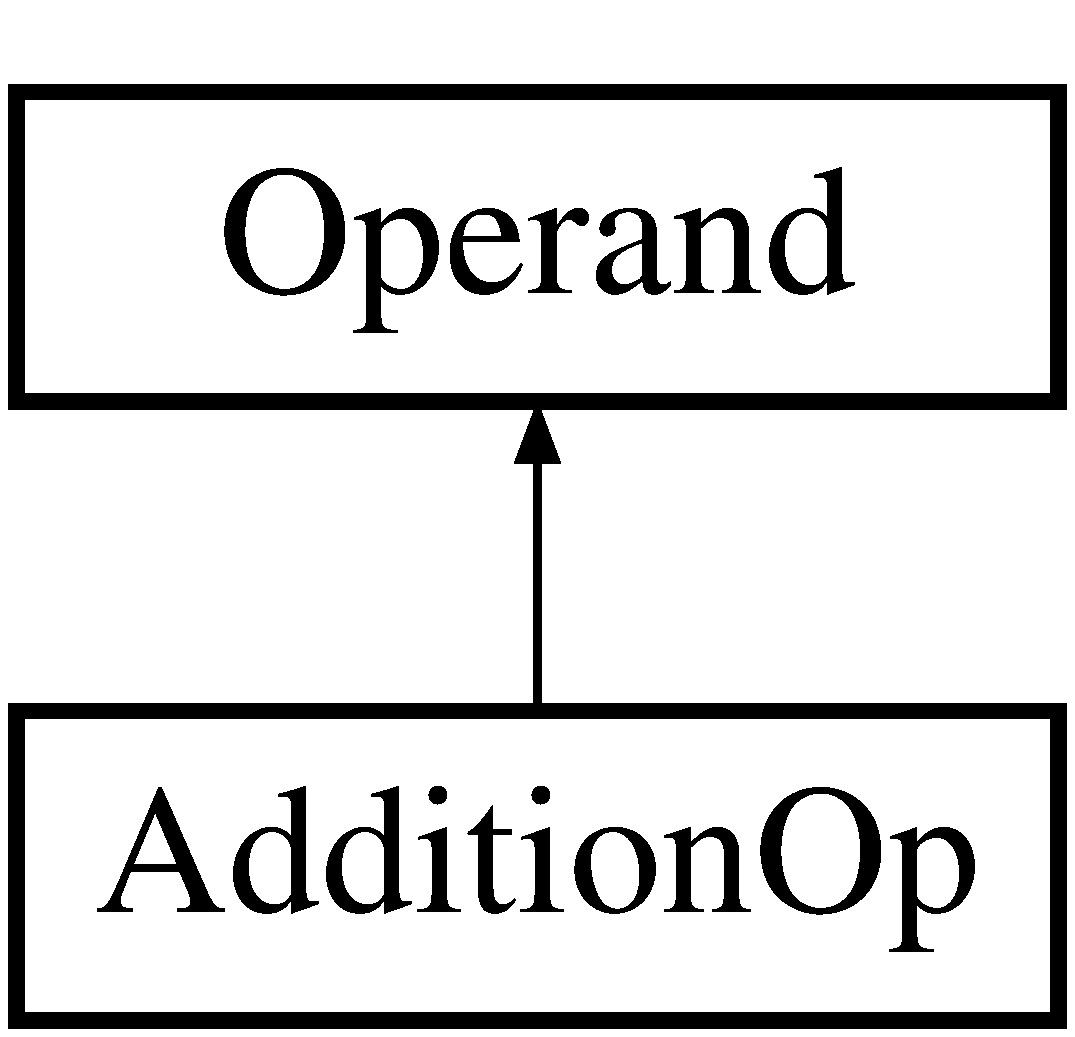
\includegraphics[height=2.000000cm]{class_addition_op}
\end{center}
\end{figure}
\subsection*{Public Member Functions}
\begin{DoxyCompactItemize}
\item 
\hyperlink{class_addition_op_a17fcc4c0a906f2dc9d177cb306f45fb3}{Addition\+Op} ()
\item 
\hyperlink{class_addition_op_a3f4c3e0a00355c7c4a2a52d121da1e91}{Addition\+Op} (std\+::vector$<$ \hyperlink{class_operand}{Operand} $\ast$ $>$ in\+Operands)
\item 
\hyperlink{class_addition_op_a840ff52a9d90e1e49c6e3f44a0af6c34}{Addition\+Op} (std\+::vector$<$ \hyperlink{class_operand}{Operand} $\ast$ $>$ in\+Operands, std\+::vector$<$ int $>$ in\+Coeffs)
\item 
virtual \hyperlink{class_symbol}{Symbol} $\ast$ \hyperlink{class_addition_op_acc5fa1937f8e82d7e6356d2aa199a5e9}{evaluate} (\hyperlink{class_symbol}{Symbol} $\ast$vars\mbox{[}$\,$\mbox{]})
\item 
virtual std\+::stringstream \hyperlink{class_addition_op_a6e62b558d233e3c358d62e14941872dc}{print} ()
\item 
virtual \hyperlink{class_addition_op}{Addition\+Op} $\ast$ \hyperlink{class_addition_op_a0339b4c06997d4592c50f9bf72f578a3}{diff} (int var\+Index)
\item 
virtual void \hyperlink{class_addition_op_aae8debc8773974054d3acf6a5df231ff}{combine\+Adds} ()
\item 
virtual void \hyperlink{class_addition_op_abd35da4badb0e1b02ab271a8f87da472}{combine\+Mults} ()
\item 
virtual void \hyperlink{class_addition_op_ad04b68e36b5852ec2b951005b71cd56d}{clean\+Mults} ()
\item 
virtual void \hyperlink{class_addition_op_a4f573734c49e2acff6ae51f15a8698d6}{clean\+Adds} ()
\item 
virtual void \hyperlink{class_addition_op_a4a0b8c6e12b6c54857b8b318c6ba55f1}{add\+Operand} (\hyperlink{class_operand}{Operand} $\ast$op)
\item 
virtual void \hyperlink{class_addition_op_a07520d850b5ab6156d278aa474e5006d}{add\+Operand} (\hyperlink{class_operand}{Operand} $\ast$op, int coeff)
\item 
std\+::vector$<$ int $>$ \hyperlink{class_addition_op_a8f952105219f850c06b9eacd352d5b0b}{get\+Coeffs} ()
\end{DoxyCompactItemize}
\subsection*{Additional Inherited Members}


\subsection{Detailed Description}


Definition at line 17 of file Addition\+Op.\+h.



\subsection{Constructor \& Destructor Documentation}
\hypertarget{class_addition_op_a17fcc4c0a906f2dc9d177cb306f45fb3}{\index{Addition\+Op@{Addition\+Op}!Addition\+Op@{Addition\+Op}}
\index{Addition\+Op@{Addition\+Op}!Addition\+Op@{Addition\+Op}}
\subsubsection[{Addition\+Op}]{\setlength{\rightskip}{0pt plus 5cm}Addition\+Op\+::\+Addition\+Op (
\begin{DoxyParamCaption}
{}
\end{DoxyParamCaption}
)\hspace{0.3cm}{\ttfamily [inline]}}}\label{class_addition_op_a17fcc4c0a906f2dc9d177cb306f45fb3}


Definition at line 23 of file Addition\+Op.\+h.

\hypertarget{class_addition_op_a3f4c3e0a00355c7c4a2a52d121da1e91}{\index{Addition\+Op@{Addition\+Op}!Addition\+Op@{Addition\+Op}}
\index{Addition\+Op@{Addition\+Op}!Addition\+Op@{Addition\+Op}}
\subsubsection[{Addition\+Op}]{\setlength{\rightskip}{0pt plus 5cm}Addition\+Op\+::\+Addition\+Op (
\begin{DoxyParamCaption}
\item[{std\+::vector$<$ {\bf Operand} $\ast$ $>$}]{in\+Operands}
\end{DoxyParamCaption}
)}}\label{class_addition_op_a3f4c3e0a00355c7c4a2a52d121da1e91}


Definition at line 25 of file Addition\+Op.\+cpp.

\hypertarget{class_addition_op_a840ff52a9d90e1e49c6e3f44a0af6c34}{\index{Addition\+Op@{Addition\+Op}!Addition\+Op@{Addition\+Op}}
\index{Addition\+Op@{Addition\+Op}!Addition\+Op@{Addition\+Op}}
\subsubsection[{Addition\+Op}]{\setlength{\rightskip}{0pt plus 5cm}Addition\+Op\+::\+Addition\+Op (
\begin{DoxyParamCaption}
\item[{std\+::vector$<$ {\bf Operand} $\ast$ $>$}]{in\+Operands, }
\item[{std\+::vector$<$ int $>$}]{in\+Coeffs}
\end{DoxyParamCaption}
)}}\label{class_addition_op_a840ff52a9d90e1e49c6e3f44a0af6c34}


Definition at line 49 of file Addition\+Op.\+cpp.



\subsection{Member Function Documentation}
\hypertarget{class_addition_op_a4a0b8c6e12b6c54857b8b318c6ba55f1}{\index{Addition\+Op@{Addition\+Op}!add\+Operand@{add\+Operand}}
\index{add\+Operand@{add\+Operand}!Addition\+Op@{Addition\+Op}}
\subsubsection[{add\+Operand}]{\setlength{\rightskip}{0pt plus 5cm}virtual void Addition\+Op\+::add\+Operand (
\begin{DoxyParamCaption}
\item[{{\bf Operand} $\ast$}]{op}
\end{DoxyParamCaption}
)\hspace{0.3cm}{\ttfamily [inline]}, {\ttfamily [virtual]}}}\label{class_addition_op_a4a0b8c6e12b6c54857b8b318c6ba55f1}


Reimplemented from \hyperlink{class_operand_aa4d004991f0b05b9b6aaa566443f63a6}{Operand}.



Definition at line 35 of file Addition\+Op.\+h.

\hypertarget{class_addition_op_a07520d850b5ab6156d278aa474e5006d}{\index{Addition\+Op@{Addition\+Op}!add\+Operand@{add\+Operand}}
\index{add\+Operand@{add\+Operand}!Addition\+Op@{Addition\+Op}}
\subsubsection[{add\+Operand}]{\setlength{\rightskip}{0pt plus 5cm}virtual void Addition\+Op\+::add\+Operand (
\begin{DoxyParamCaption}
\item[{{\bf Operand} $\ast$}]{op, }
\item[{int}]{coeff}
\end{DoxyParamCaption}
)\hspace{0.3cm}{\ttfamily [inline]}, {\ttfamily [virtual]}}}\label{class_addition_op_a07520d850b5ab6156d278aa474e5006d}


Definition at line 36 of file Addition\+Op.\+h.

\hypertarget{class_addition_op_a4f573734c49e2acff6ae51f15a8698d6}{\index{Addition\+Op@{Addition\+Op}!clean\+Adds@{clean\+Adds}}
\index{clean\+Adds@{clean\+Adds}!Addition\+Op@{Addition\+Op}}
\subsubsection[{clean\+Adds}]{\setlength{\rightskip}{0pt plus 5cm}void Addition\+Op\+::clean\+Adds (
\begin{DoxyParamCaption}
{}
\end{DoxyParamCaption}
)\hspace{0.3cm}{\ttfamily [virtual]}}}\label{class_addition_op_a4f573734c49e2acff6ae51f15a8698d6}


Implements \hyperlink{class_operand_adce551c3eaf269ed417647d9365fd8de}{Operand}.



Definition at line 374 of file Addition\+Op.\+cpp.

\hypertarget{class_addition_op_ad04b68e36b5852ec2b951005b71cd56d}{\index{Addition\+Op@{Addition\+Op}!clean\+Mults@{clean\+Mults}}
\index{clean\+Mults@{clean\+Mults}!Addition\+Op@{Addition\+Op}}
\subsubsection[{clean\+Mults}]{\setlength{\rightskip}{0pt plus 5cm}void Addition\+Op\+::clean\+Mults (
\begin{DoxyParamCaption}
{}
\end{DoxyParamCaption}
)\hspace{0.3cm}{\ttfamily [virtual]}}}\label{class_addition_op_ad04b68e36b5852ec2b951005b71cd56d}


Implements \hyperlink{class_operand_aca12745fcb2d33fda67568181eb19179}{Operand}.



Definition at line 324 of file Addition\+Op.\+cpp.

\hypertarget{class_addition_op_aae8debc8773974054d3acf6a5df231ff}{\index{Addition\+Op@{Addition\+Op}!combine\+Adds@{combine\+Adds}}
\index{combine\+Adds@{combine\+Adds}!Addition\+Op@{Addition\+Op}}
\subsubsection[{combine\+Adds}]{\setlength{\rightskip}{0pt plus 5cm}void Addition\+Op\+::combine\+Adds (
\begin{DoxyParamCaption}
{}
\end{DoxyParamCaption}
)\hspace{0.3cm}{\ttfamily [virtual]}}}\label{class_addition_op_aae8debc8773974054d3acf6a5df231ff}


Implements \hyperlink{class_operand_a1650a1adf9ed0d15423c746b6cdcdf2b}{Operand}.



Definition at line 224 of file Addition\+Op.\+cpp.

\hypertarget{class_addition_op_abd35da4badb0e1b02ab271a8f87da472}{\index{Addition\+Op@{Addition\+Op}!combine\+Mults@{combine\+Mults}}
\index{combine\+Mults@{combine\+Mults}!Addition\+Op@{Addition\+Op}}
\subsubsection[{combine\+Mults}]{\setlength{\rightskip}{0pt plus 5cm}void Addition\+Op\+::combine\+Mults (
\begin{DoxyParamCaption}
{}
\end{DoxyParamCaption}
)\hspace{0.3cm}{\ttfamily [virtual]}}}\label{class_addition_op_abd35da4badb0e1b02ab271a8f87da472}


Implements \hyperlink{class_operand_a82913d427a06d6d3f3832ce9ee0e59ff}{Operand}.



Definition at line 300 of file Addition\+Op.\+cpp.

\hypertarget{class_addition_op_a0339b4c06997d4592c50f9bf72f578a3}{\index{Addition\+Op@{Addition\+Op}!diff@{diff}}
\index{diff@{diff}!Addition\+Op@{Addition\+Op}}
\subsubsection[{diff}]{\setlength{\rightskip}{0pt plus 5cm}{\bf Addition\+Op} $\ast$ Addition\+Op\+::diff (
\begin{DoxyParamCaption}
\item[{int}]{var\+Index}
\end{DoxyParamCaption}
)\hspace{0.3cm}{\ttfamily [virtual]}}}\label{class_addition_op_a0339b4c06997d4592c50f9bf72f578a3}


Implements \hyperlink{class_operand_a057d6848e78c2cc4d36a5d57ef68fa61}{Operand}.



Definition at line 194 of file Addition\+Op.\+cpp.

\hypertarget{class_addition_op_acc5fa1937f8e82d7e6356d2aa199a5e9}{\index{Addition\+Op@{Addition\+Op}!evaluate@{evaluate}}
\index{evaluate@{evaluate}!Addition\+Op@{Addition\+Op}}
\subsubsection[{evaluate}]{\setlength{\rightskip}{0pt plus 5cm}{\bf Symbol} $\ast$ Addition\+Op\+::evaluate (
\begin{DoxyParamCaption}
\item[{{\bf Symbol} $\ast$}]{vars\mbox{[}$\,$\mbox{]}}
\end{DoxyParamCaption}
)\hspace{0.3cm}{\ttfamily [virtual]}}}\label{class_addition_op_acc5fa1937f8e82d7e6356d2aa199a5e9}


Implements \hyperlink{class_operand_a910e63f6f002b26dd75deb83af9c69a7}{Operand}.



Definition at line 71 of file Addition\+Op.\+cpp.

\hypertarget{class_addition_op_a8f952105219f850c06b9eacd352d5b0b}{\index{Addition\+Op@{Addition\+Op}!get\+Coeffs@{get\+Coeffs}}
\index{get\+Coeffs@{get\+Coeffs}!Addition\+Op@{Addition\+Op}}
\subsubsection[{get\+Coeffs}]{\setlength{\rightskip}{0pt plus 5cm}std\+::vector$<$int$>$ Addition\+Op\+::get\+Coeffs (
\begin{DoxyParamCaption}
{}
\end{DoxyParamCaption}
)\hspace{0.3cm}{\ttfamily [inline]}}}\label{class_addition_op_a8f952105219f850c06b9eacd352d5b0b}


Definition at line 39 of file Addition\+Op.\+h.

\hypertarget{class_addition_op_a6e62b558d233e3c358d62e14941872dc}{\index{Addition\+Op@{Addition\+Op}!print@{print}}
\index{print@{print}!Addition\+Op@{Addition\+Op}}
\subsubsection[{print}]{\setlength{\rightskip}{0pt plus 5cm}std\+::stringstream Addition\+Op\+::print (
\begin{DoxyParamCaption}
{}
\end{DoxyParamCaption}
)\hspace{0.3cm}{\ttfamily [virtual]}}}\label{class_addition_op_a6e62b558d233e3c358d62e14941872dc}


Implements \hyperlink{class_operand_a8cc045602e1f603a5920249a69abde03}{Operand}.



Definition at line 127 of file Addition\+Op.\+cpp.



The documentation for this class was generated from the following files\+:\begin{DoxyCompactItemize}
\item 
S\+L\+P/\hyperlink{_addition_op_8h}{Addition\+Op.\+h}\item 
S\+L\+P/\hyperlink{_addition_op_8cpp}{Addition\+Op.\+cpp}\end{DoxyCompactItemize}

\hypertarget{class_a_m_p}{\section{A\+M\+P Class Reference}
\label{class_a_m_p}\index{A\+M\+P@{A\+M\+P}}
}


{\ttfamily \#include $<$amp.\+hpp$>$}

Inheritance diagram for A\+M\+P\+:\begin{figure}[H]
\begin{center}
\leavevmode
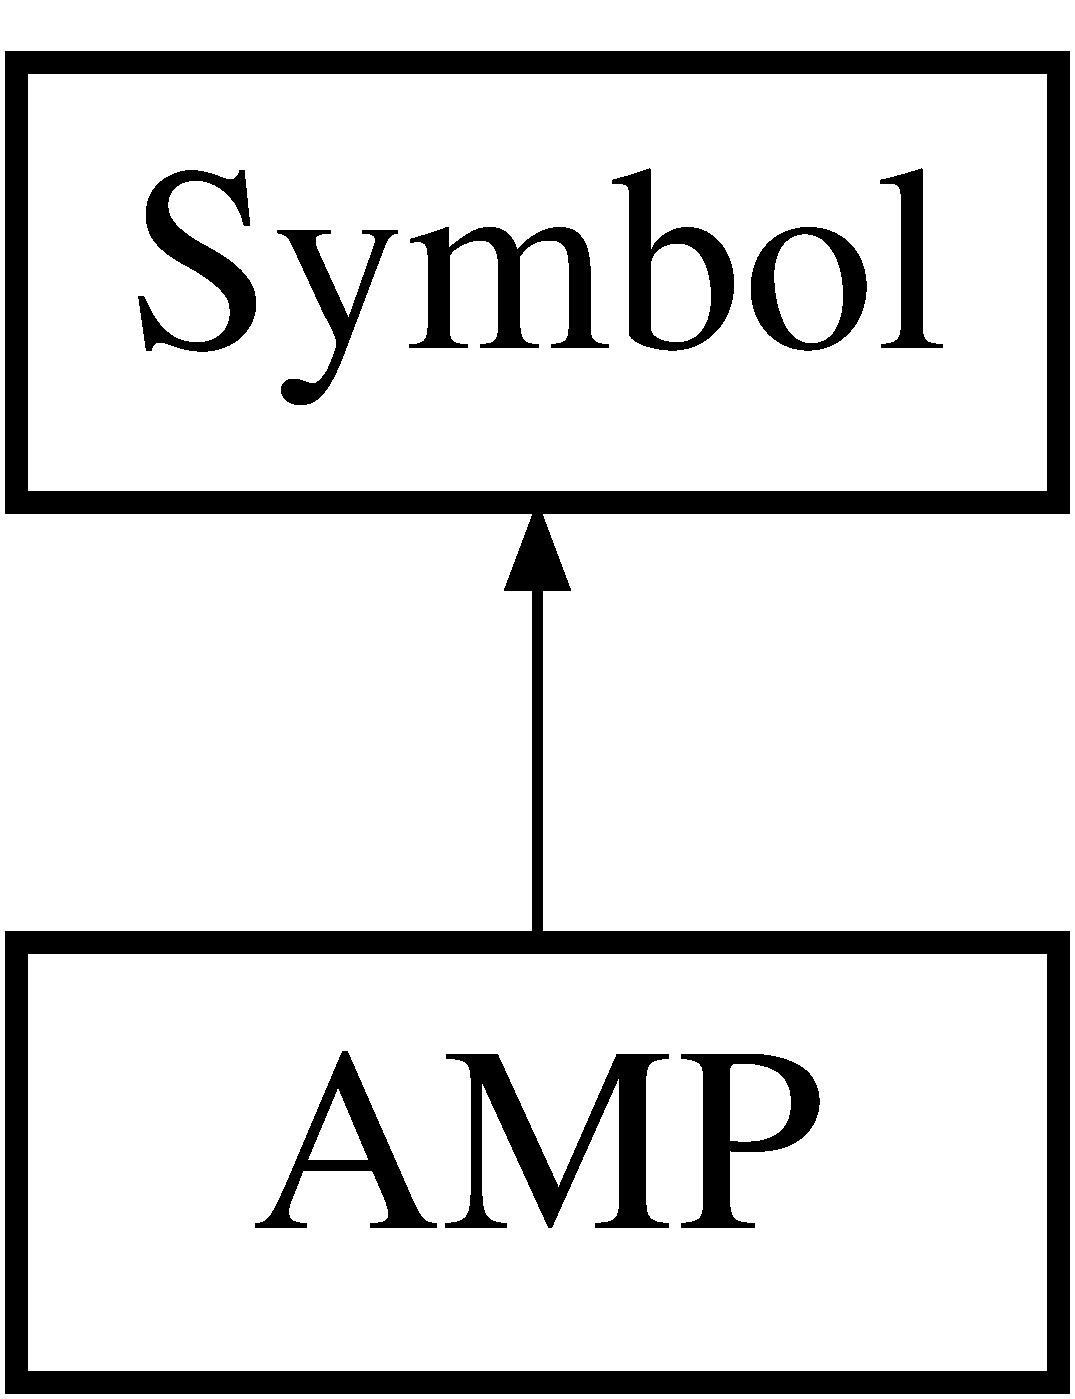
\includegraphics[height=2.000000cm]{class_a_m_p}
\end{center}
\end{figure}
\subsection*{Public Member Functions}
\begin{DoxyCompactItemize}
\item 
\hyperlink{class_a_m_p_adee66e9c3e14bcda4e0f9ad41e1e0335}{A\+M\+P} ()
\item 
\hyperlink{class_a_m_p_a481ad3a03f94b3b94568bb9eac1fb466}{A\+M\+P} (double v)
\item 
\hyperlink{class_a_m_p_af2718e09eaedb9bbf3a28bd260c6d8b6}{A\+M\+P} (std\+::string str, int base, int prec)
\item 
\hyperlink{class_a_m_p_a82233ee7f6ef6d3a60de4c26577c3dfd}{A\+M\+P} (mpfr\+\_\+t m)
\item 
\hyperlink{class_a_m_p_a8d3bb5485998c3eb4fd8440ad13ed1af}{$\sim$\+A\+M\+P} ()
\item 
\hyperlink{class_a_m_p_a1489b5bcd791211890e96be541f45693}{A\+M\+P} (\hyperlink{class_a_m_p}{A\+M\+P} \&copy\+\_\+from\+\_\+me)
\item 
\hyperlink{class_a_m_p_a979411a214a965c50b60a95eda1ea78e}{A\+M\+P} (const \hyperlink{class_a_m_p}{A\+M\+P} \&copy\+\_\+from\+\_\+me)
\item 
\hyperlink{class_a_m_p_a4a2d7e847c333daf12a1b957adbb9a62}{A\+M\+P} (volatile \hyperlink{class_a_m_p}{A\+M\+P} \&copy\+\_\+from\+\_\+me)
\item 
\hyperlink{class_a_m_p_a499d42ec7afbb99db2d9ba32cf98f98d}{A\+M\+P} (const volatile \hyperlink{class_a_m_p}{A\+M\+P} \&copy\+\_\+from\+\_\+me)
\item 
int \hyperlink{class_a_m_p_ab19be67af62d854d022ee53921953167}{Get\+Precision} ()
\item 
double $\ast$ \hyperlink{class_a_m_p_abc7e1b7d895d542da54e332ec461f07f}{Get\+D} ()
\item 
mpfr\+\_\+t $\ast$ \hyperlink{class_a_m_p_a3f39697c054b30f4637923b45aac9795}{Get\+M\+P} ()
\item 
std\+::string \hyperlink{class_a_m_p_aa376d6c4be6390e62c274eeeef4fbd12}{Get\+Stats} (std\+::string s)
\item 
bool \hyperlink{class_a_m_p_afd0da25041946d69753f2cdf6b2a5065}{Get\+Precision\+B} ()
\item 
void \hyperlink{class_a_m_p_ab098ea8e83660764f2f2110aa4ea739f}{Set\+Precision} (int prec)
\item 
void \hyperlink{class_a_m_p_a7d3f8c20b06a72cd4f7b8300aae45e6d}{Set\+Precision} (mp\+\_\+prec\+\_\+t mp\+\_\+prec)
\item 
void \hyperlink{class_a_m_p_a1a3f15f4cd90c4f97fcfe2f4fbb2e4e5}{Set} (std\+::string str, int base, int prec)
\item 
void \hyperlink{class_a_m_p_a3c0a25d70c600791f4ad22b11e462101}{Set} (mpfr\+\_\+t m)
\item 
void \hyperlink{class_a_m_p_a4d7472e47c0b5458c00fe30dff4d91d4}{Set} (double t)
\item 
\hyperlink{class_a_m_p}{A\+M\+P} \& \hyperlink{class_a_m_p_a5bbdda51e9627a6e4ec3171fce34c1b3}{operator=} (\hyperlink{class_a_m_p}{A\+M\+P} a)
\item 
virtual std\+::stringstream \hyperlink{class_a_m_p_a0d97f7941390b745d4a8c5099f8530c1}{print} ()
\item 
virtual \hyperlink{class_symbol}{Symbol} $\ast$ \hyperlink{class_a_m_p_a13330b73b85994d48e091ba35d37f5da}{add} (\hyperlink{class_symbol}{Symbol} $\ast$operand)
\item 
virtual \hyperlink{class_symbol}{Symbol} $\ast$ \hyperlink{class_a_m_p_aa22f858fe19e8d00dea47ee9a6c26040}{sub} (\hyperlink{class_symbol}{Symbol} $\ast$operand)
\item 
virtual \hyperlink{class_symbol}{Symbol} $\ast$ \hyperlink{class_a_m_p_ab9c9e14b427261284a980f936ce64095}{mult} (\hyperlink{class_symbol}{Symbol} $\ast$operand)
\item 
virtual \hyperlink{class_symbol}{Symbol} $\ast$ \hyperlink{class_a_m_p_a0c3ed1aeaa0a0974f0ea3f7f92dbe080}{exp} (int exp)
\item 
virtual \hyperlink{class_symbol}{Symbol} $\ast$ \hyperlink{class_a_m_p_aacc63b07222e5a3e1d3008ffcf8564c2}{neg} ()
\item 
virtual \hyperlink{class_a_m_p}{A\+M\+P} $\ast$ \hyperlink{class_a_m_p_a7be3cf2bc62e7849d829412cd9e83875}{clone} ()
\end{DoxyCompactItemize}
\subsection*{Friends}
\begin{DoxyCompactItemize}
\item 
\hyperlink{class_a_m_p}{A\+M\+P} \hyperlink{class_a_m_p_a53fa727ddd84247135d8242ca76c0ea5}{operator+} (\hyperlink{class_a_m_p}{A\+M\+P} a, \hyperlink{class_a_m_p}{A\+M\+P} b)
\item 
\hyperlink{class_a_m_p}{A\+M\+P} \hyperlink{class_a_m_p_ab8c006600aac3ca1d268f527fa735601}{operator+} (\hyperlink{class_a_m_p}{A\+M\+P} a, double b)
\item 
\hyperlink{class_a_m_p}{A\+M\+P} \hyperlink{class_a_m_p_a129043da29f3d738404f7677f435d08f}{operator+} (double a, \hyperlink{class_a_m_p}{A\+M\+P} b)
\item 
\hyperlink{class_a_m_p}{A\+M\+P} \hyperlink{class_a_m_p_a9dfbf753a991f63b3bbd4edefeaa09dd}{operator-\/} (\hyperlink{class_a_m_p}{A\+M\+P} a, \hyperlink{class_a_m_p}{A\+M\+P} b)
\item 
\hyperlink{class_a_m_p}{A\+M\+P} \hyperlink{class_a_m_p_a9dd9bc8a7376ca14830562409c00ce9c}{operator-\/} (\hyperlink{class_a_m_p}{A\+M\+P} a, double b)
\item 
\hyperlink{class_a_m_p}{A\+M\+P} \hyperlink{class_a_m_p_aa8ee1d36bd733990bbbba40412e3f554}{operator-\/} (double a, \hyperlink{class_a_m_p}{A\+M\+P} b)
\item 
\hyperlink{class_a_m_p}{A\+M\+P} \hyperlink{class_a_m_p_a9c2c71d0d7012e73cf03b456d95166b4}{operator$\ast$} (\hyperlink{class_a_m_p}{A\+M\+P} a, \hyperlink{class_a_m_p}{A\+M\+P} b)
\item 
\hyperlink{class_a_m_p}{A\+M\+P} \hyperlink{class_a_m_p_acb5225604989f2f4177eaec6b08c5cde}{operator$\ast$} (double a, \hyperlink{class_a_m_p}{A\+M\+P} b)
\item 
\hyperlink{class_a_m_p}{A\+M\+P} \hyperlink{class_a_m_p_a9fc5f153f95cda0dd331590738815acf}{operator$\ast$} (\hyperlink{class_a_m_p}{A\+M\+P} a, double b)
\item 
\hyperlink{class_a_m_p}{A\+M\+P} \hyperlink{class_a_m_p_a09fc3cf3b6ff3f388cfbf730cca9d216}{operator/} (\hyperlink{class_a_m_p}{A\+M\+P} a, \hyperlink{class_a_m_p}{A\+M\+P} b)
\item 
\hyperlink{class_a_m_p}{A\+M\+P} \hyperlink{class_a_m_p_a92ea228fb63190a290a22dd1f61d7084}{operator/} (\hyperlink{class_a_m_p}{A\+M\+P} a, double b)
\item 
\hyperlink{class_a_m_p}{A\+M\+P} \hyperlink{class_a_m_p_a3b58c3a64b532a6460a734b96792ec4a}{operator/} (double a, \hyperlink{class_a_m_p}{A\+M\+P} b)
\end{DoxyCompactItemize}
\subsection*{Additional Inherited Members}


\subsection{Detailed Description}


Definition at line 20 of file amp.\+hpp.



\subsection{Constructor \& Destructor Documentation}
\hypertarget{class_a_m_p_adee66e9c3e14bcda4e0f9ad41e1e0335}{\index{A\+M\+P@{A\+M\+P}!A\+M\+P@{A\+M\+P}}
\index{A\+M\+P@{A\+M\+P}!A\+M\+P@{A\+M\+P}}
\subsubsection[{A\+M\+P}]{\setlength{\rightskip}{0pt plus 5cm}A\+M\+P\+::\+A\+M\+P (
\begin{DoxyParamCaption}
{}
\end{DoxyParamCaption}
)}}\label{class_a_m_p_adee66e9c3e14bcda4e0f9ad41e1e0335}
Constructors Default Constructor. Allocate all pointers, precision, and initalize the dereferenced mpfr\+\_\+t pointer. 

Definition at line 13 of file amp.\+cpp.

\hypertarget{class_a_m_p_a481ad3a03f94b3b94568bb9eac1fb466}{\index{A\+M\+P@{A\+M\+P}!A\+M\+P@{A\+M\+P}}
\index{A\+M\+P@{A\+M\+P}!A\+M\+P@{A\+M\+P}}
\subsubsection[{A\+M\+P}]{\setlength{\rightskip}{0pt plus 5cm}A\+M\+P\+::\+A\+M\+P (
\begin{DoxyParamCaption}
\item[{double}]{v}
\end{DoxyParamCaption}
)}}\label{class_a_m_p_a481ad3a03f94b3b94568bb9eac1fb466}
Double constructor. 
\begin{DoxyParams}{Parameters}
{\em double} & v -\/ The value of the dereferenced pointer. \\
\hline
\end{DoxyParams}


Definition at line 28 of file amp.\+cpp.

\hypertarget{class_a_m_p_af2718e09eaedb9bbf3a28bd260c6d8b6}{\index{A\+M\+P@{A\+M\+P}!A\+M\+P@{A\+M\+P}}
\index{A\+M\+P@{A\+M\+P}!A\+M\+P@{A\+M\+P}}
\subsubsection[{A\+M\+P}]{\setlength{\rightskip}{0pt plus 5cm}A\+M\+P\+::\+A\+M\+P (
\begin{DoxyParamCaption}
\item[{std\+::string}]{str, }
\item[{int}]{base, }
\item[{int}]{prec}
\end{DoxyParamCaption}
)}}\label{class_a_m_p_af2718e09eaedb9bbf3a28bd260c6d8b6}
M\+P String Constructor 
\begin{DoxyParams}{Parameters}
{\em std\+::string} & -\/ the string of the constructor. \\
\hline
{\em int} & base -\/ the base of the string \\
\hline
{\em prec} & -\/ the precision in bits \\
\hline
\end{DoxyParams}


Definition at line 46 of file amp.\+cpp.

\hypertarget{class_a_m_p_a82233ee7f6ef6d3a60de4c26577c3dfd}{\index{A\+M\+P@{A\+M\+P}!A\+M\+P@{A\+M\+P}}
\index{A\+M\+P@{A\+M\+P}!A\+M\+P@{A\+M\+P}}
\subsubsection[{A\+M\+P}]{\setlength{\rightskip}{0pt plus 5cm}A\+M\+P\+::\+A\+M\+P (
\begin{DoxyParamCaption}
\item[{mpfr\+\_\+t}]{m}
\end{DoxyParamCaption}
)}}\label{class_a_m_p_a82233ee7f6ef6d3a60de4c26577c3dfd}
M\+P mpfr\+\_\+t constructor 
\begin{DoxyParams}{Parameters}
{\em mpfr\+\_\+t} & m -\/ The new value of the derefenced mp.\\
\hline
\end{DoxyParams}
M\+P mpfr\+\_\+t constructor. 
\begin{DoxyParams}{Parameters}
{\em mpfr\+\_\+t} & m -- the value of the dereferenced mp \\
\hline
\end{DoxyParams}


Definition at line 67 of file amp.\+cpp.

\hypertarget{class_a_m_p_a8d3bb5485998c3eb4fd8440ad13ed1af}{\index{A\+M\+P@{A\+M\+P}!````~A\+M\+P@{$\sim$\+A\+M\+P}}
\index{````~A\+M\+P@{$\sim$\+A\+M\+P}!A\+M\+P@{A\+M\+P}}
\subsubsection[{$\sim$\+A\+M\+P}]{\setlength{\rightskip}{0pt plus 5cm}A\+M\+P\+::$\sim$\+A\+M\+P (
\begin{DoxyParamCaption}
{}
\end{DoxyParamCaption}
)}}\label{class_a_m_p_a8d3bb5485998c3eb4fd8440ad13ed1af}
The default destructor. 

Definition at line 77 of file amp.\+cpp.

\hypertarget{class_a_m_p_a1489b5bcd791211890e96be541f45693}{\index{A\+M\+P@{A\+M\+P}!A\+M\+P@{A\+M\+P}}
\index{A\+M\+P@{A\+M\+P}!A\+M\+P@{A\+M\+P}}
\subsubsection[{A\+M\+P}]{\setlength{\rightskip}{0pt plus 5cm}A\+M\+P\+::\+A\+M\+P (
\begin{DoxyParamCaption}
\item[{{\bf A\+M\+P} \&}]{copy\+\_\+from\+\_\+me}
\end{DoxyParamCaption}
)}}\label{class_a_m_p_a1489b5bcd791211890e96be541f45693}
Copy constructors. Reference copy constructor. 

Definition at line 88 of file amp.\+cpp.

\hypertarget{class_a_m_p_a979411a214a965c50b60a95eda1ea78e}{\index{A\+M\+P@{A\+M\+P}!A\+M\+P@{A\+M\+P}}
\index{A\+M\+P@{A\+M\+P}!A\+M\+P@{A\+M\+P}}
\subsubsection[{A\+M\+P}]{\setlength{\rightskip}{0pt plus 5cm}A\+M\+P\+::\+A\+M\+P (
\begin{DoxyParamCaption}
\item[{const {\bf A\+M\+P} \&}]{copy\+\_\+from\+\_\+me}
\end{DoxyParamCaption}
)}}\label{class_a_m_p_a979411a214a965c50b60a95eda1ea78e}
Constant reference copy constructor. 

Definition at line 99 of file amp.\+cpp.

\hypertarget{class_a_m_p_a4a2d7e847c333daf12a1b957adbb9a62}{\index{A\+M\+P@{A\+M\+P}!A\+M\+P@{A\+M\+P}}
\index{A\+M\+P@{A\+M\+P}!A\+M\+P@{A\+M\+P}}
\subsubsection[{A\+M\+P}]{\setlength{\rightskip}{0pt plus 5cm}A\+M\+P\+::\+A\+M\+P (
\begin{DoxyParamCaption}
\item[{volatile {\bf A\+M\+P} \&}]{copy\+\_\+from\+\_\+me}
\end{DoxyParamCaption}
)}}\label{class_a_m_p_a4a2d7e847c333daf12a1b957adbb9a62}
Volatile reference copy constructor. 

Definition at line 109 of file amp.\+cpp.

\hypertarget{class_a_m_p_a499d42ec7afbb99db2d9ba32cf98f98d}{\index{A\+M\+P@{A\+M\+P}!A\+M\+P@{A\+M\+P}}
\index{A\+M\+P@{A\+M\+P}!A\+M\+P@{A\+M\+P}}
\subsubsection[{A\+M\+P}]{\setlength{\rightskip}{0pt plus 5cm}A\+M\+P\+::\+A\+M\+P (
\begin{DoxyParamCaption}
\item[{const volatile {\bf A\+M\+P} \&}]{copy\+\_\+from\+\_\+me}
\end{DoxyParamCaption}
)}}\label{class_a_m_p_a499d42ec7afbb99db2d9ba32cf98f98d}
Constant volatile reference copy constructor. 

Definition at line 118 of file amp.\+cpp.



\subsection{Member Function Documentation}
\hypertarget{class_a_m_p_a13330b73b85994d48e091ba35d37f5da}{\index{A\+M\+P@{A\+M\+P}!add@{add}}
\index{add@{add}!A\+M\+P@{A\+M\+P}}
\subsubsection[{add}]{\setlength{\rightskip}{0pt plus 5cm}{\bf Symbol} $\ast$ A\+M\+P\+::add (
\begin{DoxyParamCaption}
\item[{{\bf Symbol} $\ast$}]{operand}
\end{DoxyParamCaption}
)\hspace{0.3cm}{\ttfamily [virtual]}}}\label{class_a_m_p_a13330b73b85994d48e091ba35d37f5da}


Implements \hyperlink{class_symbol_ae8aeeef72df9b6c8f32197e97b909c72}{Symbol}.



Definition at line 816 of file amp.\+cpp.

\hypertarget{class_a_m_p_a7be3cf2bc62e7849d829412cd9e83875}{\index{A\+M\+P@{A\+M\+P}!clone@{clone}}
\index{clone@{clone}!A\+M\+P@{A\+M\+P}}
\subsubsection[{clone}]{\setlength{\rightskip}{0pt plus 5cm}virtual {\bf A\+M\+P}$\ast$ A\+M\+P\+::clone (
\begin{DoxyParamCaption}
{}
\end{DoxyParamCaption}
)\hspace{0.3cm}{\ttfamily [inline]}, {\ttfamily [virtual]}}}\label{class_a_m_p_a7be3cf2bc62e7849d829412cd9e83875}


Implements \hyperlink{class_symbol_a642df9ea636eb1b7fafa11fc539ea49a}{Symbol}.



Definition at line 164 of file amp.\+hpp.

\hypertarget{class_a_m_p_a0c3ed1aeaa0a0974f0ea3f7f92dbe080}{\index{A\+M\+P@{A\+M\+P}!exp@{exp}}
\index{exp@{exp}!A\+M\+P@{A\+M\+P}}
\subsubsection[{exp}]{\setlength{\rightskip}{0pt plus 5cm}{\bf Symbol} $\ast$ A\+M\+P\+::exp (
\begin{DoxyParamCaption}
\item[{int}]{exp}
\end{DoxyParamCaption}
)\hspace{0.3cm}{\ttfamily [virtual]}}}\label{class_a_m_p_a0c3ed1aeaa0a0974f0ea3f7f92dbe080}


Implements \hyperlink{class_symbol_aa259102d6727f267c718b91c78e5eb46}{Symbol}.



Definition at line 925 of file amp.\+cpp.

\hypertarget{class_a_m_p_abc7e1b7d895d542da54e332ec461f07f}{\index{A\+M\+P@{A\+M\+P}!Get\+D@{Get\+D}}
\index{Get\+D@{Get\+D}!A\+M\+P@{A\+M\+P}}
\subsubsection[{Get\+D}]{\setlength{\rightskip}{0pt plus 5cm}double$\ast$ A\+M\+P\+::\+Get\+D (
\begin{DoxyParamCaption}
{}
\end{DoxyParamCaption}
)\hspace{0.3cm}{\ttfamily [inline]}}}\label{class_a_m_p_abc7e1b7d895d542da54e332ec461f07f}
Get the pointer to the double. \begin{DoxyReturn}{Returns}
d -\/ The pointer to the double. 
\end{DoxyReturn}


Definition at line 69 of file amp.\+hpp.

\hypertarget{class_a_m_p_a3f39697c054b30f4637923b45aac9795}{\index{A\+M\+P@{A\+M\+P}!Get\+M\+P@{Get\+M\+P}}
\index{Get\+M\+P@{Get\+M\+P}!A\+M\+P@{A\+M\+P}}
\subsubsection[{Get\+M\+P}]{\setlength{\rightskip}{0pt plus 5cm}mpfr\+\_\+t$\ast$ A\+M\+P\+::\+Get\+M\+P (
\begin{DoxyParamCaption}
{}
\end{DoxyParamCaption}
)\hspace{0.3cm}{\ttfamily [inline]}}}\label{class_a_m_p_a3f39697c054b30f4637923b45aac9795}
Get the pointer to the mpfr object. \begin{DoxyReturn}{Returns}
mp -\/ The pointer to the mpfr object. 
\end{DoxyReturn}


Definition at line 74 of file amp.\+hpp.

\hypertarget{class_a_m_p_ab19be67af62d854d022ee53921953167}{\index{A\+M\+P@{A\+M\+P}!Get\+Precision@{Get\+Precision}}
\index{Get\+Precision@{Get\+Precision}!A\+M\+P@{A\+M\+P}}
\subsubsection[{Get\+Precision}]{\setlength{\rightskip}{0pt plus 5cm}int A\+M\+P\+::\+Get\+Precision (
\begin{DoxyParamCaption}
{}
\end{DoxyParamCaption}
)}}\label{class_a_m_p_ab19be67af62d854d022ee53921953167}
Get the precision. \begin{DoxyReturn}{Returns}
precision -\/ The precision in bits. 
\end{DoxyReturn}


Definition at line 133 of file amp.\+cpp.

\hypertarget{class_a_m_p_afd0da25041946d69753f2cdf6b2a5065}{\index{A\+M\+P@{A\+M\+P}!Get\+Precision\+B@{Get\+Precision\+B}}
\index{Get\+Precision\+B@{Get\+Precision\+B}!A\+M\+P@{A\+M\+P}}
\subsubsection[{Get\+Precision\+B}]{\setlength{\rightskip}{0pt plus 5cm}bool A\+M\+P\+::\+Get\+Precision\+B (
\begin{DoxyParamCaption}
{}
\end{DoxyParamCaption}
)\hspace{0.3cm}{\ttfamily [inline]}}}\label{class_a_m_p_afd0da25041946d69753f2cdf6b2a5065}
A function that returns true if using multiprecision and false when using hardware precision. 

Definition at line 83 of file amp.\+hpp.

\hypertarget{class_a_m_p_aa376d6c4be6390e62c274eeeef4fbd12}{\index{A\+M\+P@{A\+M\+P}!Get\+Stats@{Get\+Stats}}
\index{Get\+Stats@{Get\+Stats}!A\+M\+P@{A\+M\+P}}
\subsubsection[{Get\+Stats}]{\setlength{\rightskip}{0pt plus 5cm}std\+::string A\+M\+P\+::\+Get\+Stats (
\begin{DoxyParamCaption}
\item[{std\+::string}]{s}
\end{DoxyParamCaption}
)}}\label{class_a_m_p_aa376d6c4be6390e62c274eeeef4fbd12}
A function for testing purposes that returns a string object with the \hyperlink{class_a_m_p}{A\+M\+P} object's information. \begin{DoxyReturn}{Returns}
std\+::string -\/ The string that contains the information.
\end{DoxyReturn}
A function for testing purposes. returns a string with object information. 

Definition at line 283 of file amp.\+cpp.

\hypertarget{class_a_m_p_ab9c9e14b427261284a980f936ce64095}{\index{A\+M\+P@{A\+M\+P}!mult@{mult}}
\index{mult@{mult}!A\+M\+P@{A\+M\+P}}
\subsubsection[{mult}]{\setlength{\rightskip}{0pt plus 5cm}{\bf Symbol} $\ast$ A\+M\+P\+::mult (
\begin{DoxyParamCaption}
\item[{{\bf Symbol} $\ast$}]{operand}
\end{DoxyParamCaption}
)\hspace{0.3cm}{\ttfamily [virtual]}}}\label{class_a_m_p_ab9c9e14b427261284a980f936ce64095}


Implements \hyperlink{class_symbol_a224ae5c870650b7704756d8279b9bc53}{Symbol}.



Definition at line 890 of file amp.\+cpp.

\hypertarget{class_a_m_p_aacc63b07222e5a3e1d3008ffcf8564c2}{\index{A\+M\+P@{A\+M\+P}!neg@{neg}}
\index{neg@{neg}!A\+M\+P@{A\+M\+P}}
\subsubsection[{neg}]{\setlength{\rightskip}{0pt plus 5cm}{\bf Symbol} $\ast$ A\+M\+P\+::neg (
\begin{DoxyParamCaption}
{}
\end{DoxyParamCaption}
)\hspace{0.3cm}{\ttfamily [virtual]}}}\label{class_a_m_p_aacc63b07222e5a3e1d3008ffcf8564c2}


Implements \hyperlink{class_symbol_acfc77f36fef51f4d300896d0e5183986}{Symbol}.



Definition at line 932 of file amp.\+cpp.

\hypertarget{class_a_m_p_a5bbdda51e9627a6e4ec3171fce34c1b3}{\index{A\+M\+P@{A\+M\+P}!operator=@{operator=}}
\index{operator=@{operator=}!A\+M\+P@{A\+M\+P}}
\subsubsection[{operator=}]{\setlength{\rightskip}{0pt plus 5cm}{\bf A\+M\+P} \& A\+M\+P\+::operator= (
\begin{DoxyParamCaption}
\item[{{\bf A\+M\+P}}]{a}
\end{DoxyParamCaption}
)}}\label{class_a_m_p_a5bbdda51e9627a6e4ec3171fce34c1b3}
The assignment = operator. 
\begin{DoxyParams}{Parameters}
{\em \hyperlink{class_a_m_p}{A\+M\+P}} & a -\/ The value to be assigned to $\ast$this. \\
\hline
\end{DoxyParams}


Definition at line 299 of file amp.\+cpp.

\hypertarget{class_a_m_p_a0d97f7941390b745d4a8c5099f8530c1}{\index{A\+M\+P@{A\+M\+P}!print@{print}}
\index{print@{print}!A\+M\+P@{A\+M\+P}}
\subsubsection[{print}]{\setlength{\rightskip}{0pt plus 5cm}virtual std\+::stringstream A\+M\+P\+::print (
\begin{DoxyParamCaption}
{}
\end{DoxyParamCaption}
)\hspace{0.3cm}{\ttfamily [inline]}, {\ttfamily [virtual]}}}\label{class_a_m_p_a0d97f7941390b745d4a8c5099f8530c1}


Implements \hyperlink{class_symbol_a327d7b38b13102918bab2a09b8b6a303}{Symbol}.



Definition at line 156 of file amp.\+hpp.

\hypertarget{class_a_m_p_a1a3f15f4cd90c4f97fcfe2f4fbb2e4e5}{\index{A\+M\+P@{A\+M\+P}!Set@{Set}}
\index{Set@{Set}!A\+M\+P@{A\+M\+P}}
\subsubsection[{Set}]{\setlength{\rightskip}{0pt plus 5cm}void A\+M\+P\+::\+Set (
\begin{DoxyParamCaption}
\item[{std\+::string}]{str, }
\item[{int}]{base, }
\item[{int}]{prec}
\end{DoxyParamCaption}
)}}\label{class_a_m_p_a1a3f15f4cd90c4f97fcfe2f4fbb2e4e5}
Set the dereferenced mpfr\+\_\+t pointer. Uses the mpfr\+\_\+set\+\_\+str(mpfr\+\_\+t m, char$\ast$ c, int base, int prec) function from mpfr. 
\begin{DoxyParams}{Parameters}
{\em std\+::string} & str -\/ The floating represented as a string object. \\
\hline
{\em int} & base -\/ The base (i.\+e. number of symbols) of the string object \\
\hline
{\em prec} & -\/ The precision in bits. \\
\hline
\end{DoxyParams}


Definition at line 227 of file amp.\+cpp.

\hypertarget{class_a_m_p_a3c0a25d70c600791f4ad22b11e462101}{\index{A\+M\+P@{A\+M\+P}!Set@{Set}}
\index{Set@{Set}!A\+M\+P@{A\+M\+P}}
\subsubsection[{Set}]{\setlength{\rightskip}{0pt plus 5cm}void A\+M\+P\+::\+Set (
\begin{DoxyParamCaption}
\item[{mpfr\+\_\+t}]{m}
\end{DoxyParamCaption}
)}}\label{class_a_m_p_a3c0a25d70c600791f4ad22b11e462101}
Set the dereferenced mpfr\+\_\+t pointer. 
\begin{DoxyParams}{Parameters}
{\em mpfr\+\_\+t} & m -\/ The new value of the dereferenced pointer. \\
\hline
\end{DoxyParams}


Definition at line 244 of file amp.\+cpp.

\hypertarget{class_a_m_p_a4d7472e47c0b5458c00fe30dff4d91d4}{\index{A\+M\+P@{A\+M\+P}!Set@{Set}}
\index{Set@{Set}!A\+M\+P@{A\+M\+P}}
\subsubsection[{Set}]{\setlength{\rightskip}{0pt plus 5cm}void A\+M\+P\+::\+Set (
\begin{DoxyParamCaption}
\item[{double}]{t}
\end{DoxyParamCaption}
)}}\label{class_a_m_p_a4d7472e47c0b5458c00fe30dff4d91d4}
Set the dereferenced double pointer. 
\begin{DoxyParams}{Parameters}
{\em double} & t -\/ The value of the dereferenced pointer. \\
\hline
\end{DoxyParams}


Definition at line 268 of file amp.\+cpp.

\hypertarget{class_a_m_p_ab098ea8e83660764f2f2110aa4ea739f}{\index{A\+M\+P@{A\+M\+P}!Set\+Precision@{Set\+Precision}}
\index{Set\+Precision@{Set\+Precision}!A\+M\+P@{A\+M\+P}}
\subsubsection[{Set\+Precision}]{\setlength{\rightskip}{0pt plus 5cm}void A\+M\+P\+::\+Set\+Precision (
\begin{DoxyParamCaption}
\item[{int}]{prec}
\end{DoxyParamCaption}
)}}\label{class_a_m_p_ab098ea8e83660764f2f2110aa4ea739f}
Set the precision. 
\begin{DoxyParams}{Parameters}
{\em -\/} & The precision in bits.\\
\hline
\end{DoxyParams}
Set the precision. 
\begin{DoxyParams}{Parameters}
{\em int} & prec -\/ The precision in bits. \\
\hline
\end{DoxyParams}


Definition at line 153 of file amp.\+cpp.

\hypertarget{class_a_m_p_a7d3f8c20b06a72cd4f7b8300aae45e6d}{\index{A\+M\+P@{A\+M\+P}!Set\+Precision@{Set\+Precision}}
\index{Set\+Precision@{Set\+Precision}!A\+M\+P@{A\+M\+P}}
\subsubsection[{Set\+Precision}]{\setlength{\rightskip}{0pt plus 5cm}void A\+M\+P\+::\+Set\+Precision (
\begin{DoxyParamCaption}
\item[{mp\+\_\+prec\+\_\+t}]{mp\+\_\+prec}
\end{DoxyParamCaption}
)}}\label{class_a_m_p_a7d3f8c20b06a72cd4f7b8300aae45e6d}
Set the precision. 
\begin{DoxyParams}{Parameters}
{\em mpfr\+\_\+prec} & mp\+\_\+prec -\/ The precision in bits as an mpfr\+\_\+prec object.\\
\hline
\end{DoxyParams}
Set the precision. 
\begin{DoxyParams}{Parameters}
{\em mpfr\+\_\+prec} & mp\+\_\+prec -\/ The precision in bits as an mpfr\+\_\+prec object. \\
\hline
{\em bool} & b -\/ This should be true if int(mp\+\_\+prec) $<$ H\+A\+R\+D\+W\+A\+R\+E\+\_\+\+P\+R\+E\+C\+I\+S\+I\+O\+N \\
\hline
\end{DoxyParams}


Definition at line 188 of file amp.\+cpp.

\hypertarget{class_a_m_p_aa22f858fe19e8d00dea47ee9a6c26040}{\index{A\+M\+P@{A\+M\+P}!sub@{sub}}
\index{sub@{sub}!A\+M\+P@{A\+M\+P}}
\subsubsection[{sub}]{\setlength{\rightskip}{0pt plus 5cm}{\bf Symbol} $\ast$ A\+M\+P\+::sub (
\begin{DoxyParamCaption}
\item[{{\bf Symbol} $\ast$}]{operand}
\end{DoxyParamCaption}
)\hspace{0.3cm}{\ttfamily [virtual]}}}\label{class_a_m_p_aa22f858fe19e8d00dea47ee9a6c26040}


Implements \hyperlink{class_symbol_a53b98ce639c66d1b2e73992f20f56c54}{Symbol}.



Definition at line 851 of file amp.\+cpp.



\subsection{Friends And Related Function Documentation}
\hypertarget{class_a_m_p_a9c2c71d0d7012e73cf03b456d95166b4}{\index{A\+M\+P@{A\+M\+P}!operator$\ast$@{operator$\ast$}}
\index{operator$\ast$@{operator$\ast$}!A\+M\+P@{A\+M\+P}}
\subsubsection[{operator$\ast$}]{\setlength{\rightskip}{0pt plus 5cm}{\bf A\+M\+P} operator$\ast$ (
\begin{DoxyParamCaption}
\item[{{\bf A\+M\+P}}]{a, }
\item[{{\bf A\+M\+P}}]{b}
\end{DoxyParamCaption}
)\hspace{0.3cm}{\ttfamily [friend]}}}\label{class_a_m_p_a9c2c71d0d7012e73cf03b456d95166b4}
Multiplication operator. 

Definition at line 528 of file amp.\+cpp.

\hypertarget{class_a_m_p_acb5225604989f2f4177eaec6b08c5cde}{\index{A\+M\+P@{A\+M\+P}!operator$\ast$@{operator$\ast$}}
\index{operator$\ast$@{operator$\ast$}!A\+M\+P@{A\+M\+P}}
\subsubsection[{operator$\ast$}]{\setlength{\rightskip}{0pt plus 5cm}{\bf A\+M\+P} operator$\ast$ (
\begin{DoxyParamCaption}
\item[{double}]{a, }
\item[{{\bf A\+M\+P}}]{b}
\end{DoxyParamCaption}
)\hspace{0.3cm}{\ttfamily [friend]}}}\label{class_a_m_p_acb5225604989f2f4177eaec6b08c5cde}


Definition at line 655 of file amp.\+cpp.

\hypertarget{class_a_m_p_a9fc5f153f95cda0dd331590738815acf}{\index{A\+M\+P@{A\+M\+P}!operator$\ast$@{operator$\ast$}}
\index{operator$\ast$@{operator$\ast$}!A\+M\+P@{A\+M\+P}}
\subsubsection[{operator$\ast$}]{\setlength{\rightskip}{0pt plus 5cm}{\bf A\+M\+P} operator$\ast$ (
\begin{DoxyParamCaption}
\item[{{\bf A\+M\+P}}]{a, }
\item[{double}]{b}
\end{DoxyParamCaption}
)\hspace{0.3cm}{\ttfamily [friend]}}}\label{class_a_m_p_a9fc5f153f95cda0dd331590738815acf}


Definition at line 690 of file amp.\+cpp.

\hypertarget{class_a_m_p_a53fa727ddd84247135d8242ca76c0ea5}{\index{A\+M\+P@{A\+M\+P}!operator+@{operator+}}
\index{operator+@{operator+}!A\+M\+P@{A\+M\+P}}
\subsubsection[{operator+}]{\setlength{\rightskip}{0pt plus 5cm}{\bf A\+M\+P} operator+ (
\begin{DoxyParamCaption}
\item[{{\bf A\+M\+P}}]{a, }
\item[{{\bf A\+M\+P}}]{b}
\end{DoxyParamCaption}
)\hspace{0.3cm}{\ttfamily [friend]}}}\label{class_a_m_p_a53fa727ddd84247135d8242ca76c0ea5}
Addition operator.

Extraction operator. Addition operator. 

Definition at line 387 of file amp.\+cpp.

\hypertarget{class_a_m_p_ab8c006600aac3ca1d268f527fa735601}{\index{A\+M\+P@{A\+M\+P}!operator+@{operator+}}
\index{operator+@{operator+}!A\+M\+P@{A\+M\+P}}
\subsubsection[{operator+}]{\setlength{\rightskip}{0pt plus 5cm}{\bf A\+M\+P} operator+ (
\begin{DoxyParamCaption}
\item[{{\bf A\+M\+P}}]{a, }
\item[{double}]{b}
\end{DoxyParamCaption}
)\hspace{0.3cm}{\ttfamily [friend]}}}\label{class_a_m_p_ab8c006600aac3ca1d268f527fa735601}


Definition at line 443 of file amp.\+cpp.

\hypertarget{class_a_m_p_a129043da29f3d738404f7677f435d08f}{\index{A\+M\+P@{A\+M\+P}!operator+@{operator+}}
\index{operator+@{operator+}!A\+M\+P@{A\+M\+P}}
\subsubsection[{operator+}]{\setlength{\rightskip}{0pt plus 5cm}{\bf A\+M\+P} operator+ (
\begin{DoxyParamCaption}
\item[{double}]{a, }
\item[{{\bf A\+M\+P}}]{b}
\end{DoxyParamCaption}
)\hspace{0.3cm}{\ttfamily [friend]}}}\label{class_a_m_p_a129043da29f3d738404f7677f435d08f}


Definition at line 477 of file amp.\+cpp.

\hypertarget{class_a_m_p_a9dfbf753a991f63b3bbd4edefeaa09dd}{\index{A\+M\+P@{A\+M\+P}!operator-\/@{operator-\/}}
\index{operator-\/@{operator-\/}!A\+M\+P@{A\+M\+P}}
\subsubsection[{operator-\/}]{\setlength{\rightskip}{0pt plus 5cm}{\bf A\+M\+P} operator-\/ (
\begin{DoxyParamCaption}
\item[{{\bf A\+M\+P}}]{a, }
\item[{{\bf A\+M\+P}}]{b}
\end{DoxyParamCaption}
)\hspace{0.3cm}{\ttfamily [friend]}}}\label{class_a_m_p_a9dfbf753a991f63b3bbd4edefeaa09dd}
Subtraction operator. 

Definition at line 483 of file amp.\+cpp.

\hypertarget{class_a_m_p_a9dd9bc8a7376ca14830562409c00ce9c}{\index{A\+M\+P@{A\+M\+P}!operator-\/@{operator-\/}}
\index{operator-\/@{operator-\/}!A\+M\+P@{A\+M\+P}}
\subsubsection[{operator-\/}]{\setlength{\rightskip}{0pt plus 5cm}{\bf A\+M\+P} operator-\/ (
\begin{DoxyParamCaption}
\item[{{\bf A\+M\+P}}]{a, }
\item[{double}]{b}
\end{DoxyParamCaption}
)\hspace{0.3cm}{\ttfamily [friend]}}}\label{class_a_m_p_a9dd9bc8a7376ca14830562409c00ce9c}


Definition at line 615 of file amp.\+cpp.

\hypertarget{class_a_m_p_aa8ee1d36bd733990bbbba40412e3f554}{\index{A\+M\+P@{A\+M\+P}!operator-\/@{operator-\/}}
\index{operator-\/@{operator-\/}!A\+M\+P@{A\+M\+P}}
\subsubsection[{operator-\/}]{\setlength{\rightskip}{0pt plus 5cm}{\bf A\+M\+P} operator-\/ (
\begin{DoxyParamCaption}
\item[{double}]{a, }
\item[{{\bf A\+M\+P}}]{b}
\end{DoxyParamCaption}
)\hspace{0.3cm}{\ttfamily [friend]}}}\label{class_a_m_p_aa8ee1d36bd733990bbbba40412e3f554}


Definition at line 577 of file amp.\+cpp.

\hypertarget{class_a_m_p_a09fc3cf3b6ff3f388cfbf730cca9d216}{\index{A\+M\+P@{A\+M\+P}!operator/@{operator/}}
\index{operator/@{operator/}!A\+M\+P@{A\+M\+P}}
\subsubsection[{operator/}]{\setlength{\rightskip}{0pt plus 5cm}{\bf A\+M\+P} operator/ (
\begin{DoxyParamCaption}
\item[{{\bf A\+M\+P}}]{a, }
\item[{{\bf A\+M\+P}}]{b}
\end{DoxyParamCaption}
)\hspace{0.3cm}{\ttfamily [friend]}}}\label{class_a_m_p_a09fc3cf3b6ff3f388cfbf730cca9d216}
Division operator. 

Definition at line 698 of file amp.\+cpp.

\hypertarget{class_a_m_p_a92ea228fb63190a290a22dd1f61d7084}{\index{A\+M\+P@{A\+M\+P}!operator/@{operator/}}
\index{operator/@{operator/}!A\+M\+P@{A\+M\+P}}
\subsubsection[{operator/}]{\setlength{\rightskip}{0pt plus 5cm}{\bf A\+M\+P} operator/ (
\begin{DoxyParamCaption}
\item[{{\bf A\+M\+P}}]{a, }
\item[{double}]{b}
\end{DoxyParamCaption}
)\hspace{0.3cm}{\ttfamily [friend]}}}\label{class_a_m_p_a92ea228fb63190a290a22dd1f61d7084}


Definition at line 776 of file amp.\+cpp.

\hypertarget{class_a_m_p_a3b58c3a64b532a6460a734b96792ec4a}{\index{A\+M\+P@{A\+M\+P}!operator/@{operator/}}
\index{operator/@{operator/}!A\+M\+P@{A\+M\+P}}
\subsubsection[{operator/}]{\setlength{\rightskip}{0pt plus 5cm}{\bf A\+M\+P} operator/ (
\begin{DoxyParamCaption}
\item[{double}]{a, }
\item[{{\bf A\+M\+P}}]{b}
\end{DoxyParamCaption}
)\hspace{0.3cm}{\ttfamily [friend]}}}\label{class_a_m_p_a3b58c3a64b532a6460a734b96792ec4a}


Definition at line 748 of file amp.\+cpp.



The documentation for this class was generated from the following files\+:\begin{DoxyCompactItemize}
\item 
S\+L\+P/\hyperlink{amp_8hpp}{amp.\+hpp}\item 
S\+L\+P/\hyperlink{amp_8cpp}{amp.\+cpp}\end{DoxyCompactItemize}

\hypertarget{classbertinivector}{\section{bertinivector$<$ T $>$ Class Template Reference}
\label{classbertinivector}\index{bertinivector$<$ T $>$@{bertinivector$<$ T $>$}}
}


{\ttfamily \#include $<$bertinivector.\+h$>$}

\subsection*{Public Member Functions}
\begin{DoxyCompactItemize}
\item 
\hyperlink{classbertinivector_a4e4d4646946cecd0d131151ea63bf4b3}{bertinivector} ()
\item 
\hyperlink{classbertinivector_afc27cef039c8901c7df12256b836f7ba}{bertinivector} (int i)
\item 
\hyperlink{classbertinivector_a60b237a859adc1a28b22e9fe9575c9e9}{bertinivector} (const \hyperlink{classbertinivector}{bertinivector} \&)
\item 
void \hyperlink{classbertinivector_add1d276c73126f5c3742a79baddda86e}{push\+\_\+back} (T)
\item 
int \hyperlink{classbertinivector_a2b9a646cf9fca4ad7174503d8f5212b7}{size} ()
\item 
T \hyperlink{classbertinivector_abc1f1760611307c8d3e8f821a5b9e6b9}{operator\mbox{[}$\,$\mbox{]}} (int)
\item 
\hyperlink{classbertinivector}{bertinivector} \hyperlink{classbertinivector_a11a60de57c2abd4cbfdcf6b1a878299c}{operator+=} (const T \&)
\item 
\hyperlink{classbertinivector}{bertinivector} \hyperlink{classbertinivector_a74d1c6e0f5db23fc938f067fd272fd5e}{operator+=} (const \hyperlink{classbertinivector}{bertinivector} \&)
\item 
\hyperlink{classbertinivector}{bertinivector} \hyperlink{classbertinivector_af8619aadc7a501813553c26e3bd661e0}{operator+} (const \hyperlink{classbertinivector}{bertinivector} \&)
\item 
\hyperlink{classbertinivector}{bertinivector} \hyperlink{classbertinivector_afc122f5a018555b8666c214785b90471}{operator-\/} (const \hyperlink{classbertinivector}{bertinivector} \&)
\item 
\hyperlink{classbertinivector}{bertinivector} \hyperlink{classbertinivector_a2269c44a9db2d5cc758b4f4831488488}{operator$\ast$} (const \hyperlink{classbertinivector}{bertinivector} \&)
\item 
T \hyperlink{classbertinivector_ac03f4fb26536a56cacb97b3123bfc176}{l2norm} ()
\item 
T \hyperlink{classbertinivector_a389f6369d9fcf4386526caf01492bcc0}{l2norm\+\_\+sqrt} ()
\item 
T \hyperlink{classbertinivector_a1e44b59814fb464dd9f141312f747204}{s\+\_\+mult} (const \hyperlink{classbertinivector}{bertinivector} \&)
\item 
\hyperlink{classbertinivector}{bertinivector} \hyperlink{classbertinivector_aa1a165c356b5c62524bf37dc6fdb00b2}{operator=} (const \hyperlink{classbertinivector}{bertinivector} \&)
\item 
T \hyperlink{classbertinivector_a30295ae69152e3a5091237104276647c}{at} (int i)
\item 
virtual \hyperlink{classbertinivector_a59ba5d1fe59d831df787aa3d5d030bcc}{$\sim$bertinivector} ()
\end{DoxyCompactItemize}


\subsection{Detailed Description}
\subsubsection*{template$<$class T$>$class bertinivector$<$ T $>$}



Definition at line 11 of file bertinivector.\+h.



\subsection{Constructor \& Destructor Documentation}
\hypertarget{classbertinivector_a4e4d4646946cecd0d131151ea63bf4b3}{\index{bertinivector@{bertinivector}!bertinivector@{bertinivector}}
\index{bertinivector@{bertinivector}!bertinivector@{bertinivector}}
\subsubsection[{bertinivector}]{\setlength{\rightskip}{0pt plus 5cm}template$<$class T $>$ {\bf bertinivector}$<$ T $>$\+::{\bf bertinivector} (
\begin{DoxyParamCaption}
{}
\end{DoxyParamCaption}
)}}\label{classbertinivector_a4e4d4646946cecd0d131151ea63bf4b3}


Definition at line 13 of file bertinivector.\+cpp.

\hypertarget{classbertinivector_afc27cef039c8901c7df12256b836f7ba}{\index{bertinivector@{bertinivector}!bertinivector@{bertinivector}}
\index{bertinivector@{bertinivector}!bertinivector@{bertinivector}}
\subsubsection[{bertinivector}]{\setlength{\rightskip}{0pt plus 5cm}template$<$class T $>$ {\bf bertinivector}$<$ T $>$\+::{\bf bertinivector} (
\begin{DoxyParamCaption}
\item[{int}]{i}
\end{DoxyParamCaption}
)}}\label{classbertinivector_afc27cef039c8901c7df12256b836f7ba}


Definition at line 20 of file bertinivector.\+cpp.

\hypertarget{classbertinivector_a60b237a859adc1a28b22e9fe9575c9e9}{\index{bertinivector@{bertinivector}!bertinivector@{bertinivector}}
\index{bertinivector@{bertinivector}!bertinivector@{bertinivector}}
\subsubsection[{bertinivector}]{\setlength{\rightskip}{0pt plus 5cm}template$<$class T $>$ {\bf bertinivector}$<$ T $>$\+::{\bf bertinivector} (
\begin{DoxyParamCaption}
\item[{const {\bf bertinivector}$<$ T $>$ \&}]{v}
\end{DoxyParamCaption}
)}}\label{classbertinivector_a60b237a859adc1a28b22e9fe9575c9e9}


Definition at line 27 of file bertinivector.\+cpp.

\hypertarget{classbertinivector_a59ba5d1fe59d831df787aa3d5d030bcc}{\index{bertinivector@{bertinivector}!````~bertinivector@{$\sim$bertinivector}}
\index{````~bertinivector@{$\sim$bertinivector}!bertinivector@{bertinivector}}
\subsubsection[{$\sim$bertinivector}]{\setlength{\rightskip}{0pt plus 5cm}template$<$class T $>$ {\bf bertinivector}$<$ T $>$\+::$\sim${\bf bertinivector} (
\begin{DoxyParamCaption}
{}
\end{DoxyParamCaption}
)\hspace{0.3cm}{\ttfamily [virtual]}}}\label{classbertinivector_a59ba5d1fe59d831df787aa3d5d030bcc}


Definition at line 36 of file bertinivector.\+cpp.



\subsection{Member Function Documentation}
\hypertarget{classbertinivector_a30295ae69152e3a5091237104276647c}{\index{bertinivector@{bertinivector}!at@{at}}
\index{at@{at}!bertinivector@{bertinivector}}
\subsubsection[{at}]{\setlength{\rightskip}{0pt plus 5cm}template$<$class T $>$ T {\bf bertinivector}$<$ T $>$\+::at (
\begin{DoxyParamCaption}
\item[{int}]{i}
\end{DoxyParamCaption}
)}}\label{classbertinivector_a30295ae69152e3a5091237104276647c}


Definition at line 54 of file bertinivector.\+cpp.

\hypertarget{classbertinivector_ac03f4fb26536a56cacb97b3123bfc176}{\index{bertinivector@{bertinivector}!l2norm@{l2norm}}
\index{l2norm@{l2norm}!bertinivector@{bertinivector}}
\subsubsection[{l2norm}]{\setlength{\rightskip}{0pt plus 5cm}template$<$class T $>$ T {\bf bertinivector}$<$ T $>$\+::l2norm (
\begin{DoxyParamCaption}
{}
\end{DoxyParamCaption}
)}}\label{classbertinivector_ac03f4fb26536a56cacb97b3123bfc176}


Definition at line 151 of file bertinivector.\+cpp.

\hypertarget{classbertinivector_a389f6369d9fcf4386526caf01492bcc0}{\index{bertinivector@{bertinivector}!l2norm\+\_\+sqrt@{l2norm\+\_\+sqrt}}
\index{l2norm\+\_\+sqrt@{l2norm\+\_\+sqrt}!bertinivector@{bertinivector}}
\subsubsection[{l2norm\+\_\+sqrt}]{\setlength{\rightskip}{0pt plus 5cm}template$<$class T $>$ T {\bf bertinivector}$<$ T $>$\+::l2norm\+\_\+sqrt (
\begin{DoxyParamCaption}
{}
\end{DoxyParamCaption}
)}}\label{classbertinivector_a389f6369d9fcf4386526caf01492bcc0}


Definition at line 161 of file bertinivector.\+cpp.

\hypertarget{classbertinivector_a2269c44a9db2d5cc758b4f4831488488}{\index{bertinivector@{bertinivector}!operator$\ast$@{operator$\ast$}}
\index{operator$\ast$@{operator$\ast$}!bertinivector@{bertinivector}}
\subsubsection[{operator$\ast$}]{\setlength{\rightskip}{0pt plus 5cm}template$<$class T $>$ {\bf bertinivector}$<$ T $>$ {\bf bertinivector}$<$ T $>$\+::operator$\ast$ (
\begin{DoxyParamCaption}
\item[{const {\bf bertinivector}$<$ T $>$ \&}]{v}
\end{DoxyParamCaption}
)}}\label{classbertinivector_a2269c44a9db2d5cc758b4f4831488488}


Definition at line 121 of file bertinivector.\+cpp.

\hypertarget{classbertinivector_af8619aadc7a501813553c26e3bd661e0}{\index{bertinivector@{bertinivector}!operator+@{operator+}}
\index{operator+@{operator+}!bertinivector@{bertinivector}}
\subsubsection[{operator+}]{\setlength{\rightskip}{0pt plus 5cm}template$<$class T $>$ {\bf bertinivector}$<$ T $>$ {\bf bertinivector}$<$ T $>$\+::operator+ (
\begin{DoxyParamCaption}
\item[{const {\bf bertinivector}$<$ T $>$ \&}]{v}
\end{DoxyParamCaption}
)}}\label{classbertinivector_af8619aadc7a501813553c26e3bd661e0}


Definition at line 91 of file bertinivector.\+cpp.

\hypertarget{classbertinivector_a11a60de57c2abd4cbfdcf6b1a878299c}{\index{bertinivector@{bertinivector}!operator+=@{operator+=}}
\index{operator+=@{operator+=}!bertinivector@{bertinivector}}
\subsubsection[{operator+=}]{\setlength{\rightskip}{0pt plus 5cm}template$<$class T $>$ {\bf bertinivector}$<$ T $>$ {\bf bertinivector}$<$ T $>$\+::operator+= (
\begin{DoxyParamCaption}
\item[{const T \&}]{i}
\end{DoxyParamCaption}
)}}\label{classbertinivector_a11a60de57c2abd4cbfdcf6b1a878299c}


Definition at line 76 of file bertinivector.\+cpp.

\hypertarget{classbertinivector_a74d1c6e0f5db23fc938f067fd272fd5e}{\index{bertinivector@{bertinivector}!operator+=@{operator+=}}
\index{operator+=@{operator+=}!bertinivector@{bertinivector}}
\subsubsection[{operator+=}]{\setlength{\rightskip}{0pt plus 5cm}template$<$class T $>$ {\bf bertinivector}$<$ T $>$ {\bf bertinivector}$<$ T $>$\+::operator+= (
\begin{DoxyParamCaption}
\item[{const {\bf bertinivector}$<$ T $>$ \&}]{v}
\end{DoxyParamCaption}
)}}\label{classbertinivector_a74d1c6e0f5db23fc938f067fd272fd5e}


Definition at line 83 of file bertinivector.\+cpp.

\hypertarget{classbertinivector_afc122f5a018555b8666c214785b90471}{\index{bertinivector@{bertinivector}!operator-\/@{operator-\/}}
\index{operator-\/@{operator-\/}!bertinivector@{bertinivector}}
\subsubsection[{operator-\/}]{\setlength{\rightskip}{0pt plus 5cm}template$<$class T $>$ {\bf bertinivector}$<$ T $>$ {\bf bertinivector}$<$ T $>$\+::operator-\/ (
\begin{DoxyParamCaption}
\item[{const {\bf bertinivector}$<$ T $>$ \&}]{v}
\end{DoxyParamCaption}
)}}\label{classbertinivector_afc122f5a018555b8666c214785b90471}


Definition at line 106 of file bertinivector.\+cpp.

\hypertarget{classbertinivector_aa1a165c356b5c62524bf37dc6fdb00b2}{\index{bertinivector@{bertinivector}!operator=@{operator=}}
\index{operator=@{operator=}!bertinivector@{bertinivector}}
\subsubsection[{operator=}]{\setlength{\rightskip}{0pt plus 5cm}template$<$class T $>$ {\bf bertinivector}$<$ T $>$ {\bf bertinivector}$<$ T $>$\+::operator= (
\begin{DoxyParamCaption}
\item[{const {\bf bertinivector}$<$ T $>$ \&}]{v}
\end{DoxyParamCaption}
)}}\label{classbertinivector_aa1a165c356b5c62524bf37dc6fdb00b2}


Definition at line 172 of file bertinivector.\+cpp.

\hypertarget{classbertinivector_abc1f1760611307c8d3e8f821a5b9e6b9}{\index{bertinivector@{bertinivector}!operator\mbox{[}$\,$\mbox{]}@{operator[]}}
\index{operator\mbox{[}$\,$\mbox{]}@{operator[]}!bertinivector@{bertinivector}}
\subsubsection[{operator[]}]{\setlength{\rightskip}{0pt plus 5cm}template$<$class T $>$ T {\bf bertinivector}$<$ T $>$\+::operator\mbox{[}$\,$\mbox{]} (
\begin{DoxyParamCaption}
\item[{int}]{i}
\end{DoxyParamCaption}
)}}\label{classbertinivector_abc1f1760611307c8d3e8f821a5b9e6b9}


Definition at line 49 of file bertinivector.\+cpp.

\hypertarget{classbertinivector_add1d276c73126f5c3742a79baddda86e}{\index{bertinivector@{bertinivector}!push\+\_\+back@{push\+\_\+back}}
\index{push\+\_\+back@{push\+\_\+back}!bertinivector@{bertinivector}}
\subsubsection[{push\+\_\+back}]{\setlength{\rightskip}{0pt plus 5cm}template$<$class T $>$ void {\bf bertinivector}$<$ T $>$\+::push\+\_\+back (
\begin{DoxyParamCaption}
\item[{T}]{i}
\end{DoxyParamCaption}
)}}\label{classbertinivector_add1d276c73126f5c3742a79baddda86e}


Definition at line 41 of file bertinivector.\+cpp.

\hypertarget{classbertinivector_a1e44b59814fb464dd9f141312f747204}{\index{bertinivector@{bertinivector}!s\+\_\+mult@{s\+\_\+mult}}
\index{s\+\_\+mult@{s\+\_\+mult}!bertinivector@{bertinivector}}
\subsubsection[{s\+\_\+mult}]{\setlength{\rightskip}{0pt plus 5cm}template$<$class T $>$ T {\bf bertinivector}$<$ T $>$\+::s\+\_\+mult (
\begin{DoxyParamCaption}
\item[{const {\bf bertinivector}$<$ T $>$ \&}]{v}
\end{DoxyParamCaption}
)}}\label{classbertinivector_a1e44b59814fb464dd9f141312f747204}


Definition at line 136 of file bertinivector.\+cpp.

\hypertarget{classbertinivector_a2b9a646cf9fca4ad7174503d8f5212b7}{\index{bertinivector@{bertinivector}!size@{size}}
\index{size@{size}!bertinivector@{bertinivector}}
\subsubsection[{size}]{\setlength{\rightskip}{0pt plus 5cm}template$<$class T $>$ int {\bf bertinivector}$<$ T $>$\+::size (
\begin{DoxyParamCaption}
{}
\end{DoxyParamCaption}
)}}\label{classbertinivector_a2b9a646cf9fca4ad7174503d8f5212b7}


Definition at line 71 of file bertinivector.\+cpp.



The documentation for this class was generated from the following files\+:\begin{DoxyCompactItemize}
\item 
\hyperlink{bertinivector_8h}{bertinivector.\+h}\item 
\hyperlink{bertinivector_8cpp}{bertinivector.\+cpp}\end{DoxyCompactItemize}

\hypertarget{class_complex_a_m_p}{\section{Complex\+A\+M\+P Class Reference}
\label{class_complex_a_m_p}\index{Complex\+A\+M\+P@{Complex\+A\+M\+P}}
}


{\ttfamily \#include $<$complex\+\_\+amp.\+hpp$>$}

\subsection*{Public Member Functions}
\begin{DoxyCompactItemize}
\item 
\hyperlink{class_complex_a_m_p_a761e3ad1cffb6b430c9506350daeee7c}{Complex\+A\+M\+P} ()
\item 
\hyperlink{class_complex_a_m_p_a2e4e3a1c65d6255d7403dcf779fdc56f}{Complex\+A\+M\+P} (\hyperlink{class_a_m_p}{A\+M\+P} r, \hyperlink{class_a_m_p}{A\+M\+P} i)
\item 
\hyperlink{class_complex_a_m_p_a03a6196657f98a6b03e186f270edf6a4}{Complex\+A\+M\+P} (mpfr\+\_\+t mp\+\_\+r, mpfr\+\_\+t mp\+\_\+i)
\item 
\hyperlink{class_complex_a_m_p_a9e2cf3c6757e669b0c5e3c0a5a5c4bce}{Complex\+A\+M\+P} (double r, double i)
\item 
\hyperlink{class_complex_a_m_p_aa00c27201d3c690df6c40de6e587ab22}{$\sim$\+Complex\+A\+M\+P} ()
\item 
\hyperlink{class_complex_a_m_p_a61b4ce319592d4d298d8ab0082f95a92}{Complex\+A\+M\+P} (\hyperlink{class_complex_a_m_p}{Complex\+A\+M\+P} \&copy\+\_\+from\+\_\+me)
\item 
\hyperlink{class_complex_a_m_p_adb4464a3f59098b37b2109a12f9f33df}{Complex\+A\+M\+P} (const \hyperlink{class_complex_a_m_p}{Complex\+A\+M\+P} \&copy\+\_\+from\+\_\+me)
\item 
\hyperlink{class_complex_a_m_p_a880a526fcb17d87111cfe461fb705543}{Complex\+A\+M\+P} (volatile \hyperlink{class_complex_a_m_p}{Complex\+A\+M\+P} \&copy\+\_\+from\+\_\+me)
\item 
\hyperlink{class_complex_a_m_p_a58c83fe476969c9c3cf871ca3e214181}{Complex\+A\+M\+P} (const volatile \hyperlink{class_complex_a_m_p}{Complex\+A\+M\+P} \&copy\+\_\+from\+\_\+me)
\item 
\hyperlink{class_complex_a_m_p}{Complex\+A\+M\+P} \hyperlink{class_complex_a_m_p_a1716f29c710221dd573f5e76b1bd34ee}{Conjugate} ()
\item 
\hyperlink{class_a_m_p}{A\+M\+P} \hyperlink{class_complex_a_m_p_a1619171701c1c4a2197089eb4e4de7e4}{Norm\+Squared} ()
\item 
std\+::string \hyperlink{class_complex_a_m_p_a84b1541f74031f73148a13bf7f767fda}{Get\+Stats} (std\+::string s)
\item 
int \hyperlink{class_complex_a_m_p_a6c996530938a3f1a1404a341592c8b23}{Get\+Real\+Precision} ()
\item 
int \hyperlink{class_complex_a_m_p_a9856f877e22bb67158b05f98a38f2ccf}{Get\+Imag\+Precision} ()
\item 
\hyperlink{class_a_m_p}{A\+M\+P} $\ast$ \hyperlink{class_complex_a_m_p_a0bfcde48569256c228b65e7512fdb89f}{Get\+Real} ()
\item 
\hyperlink{class_a_m_p}{A\+M\+P} $\ast$ \hyperlink{class_complex_a_m_p_a35d1272197c25f115584ce76276114b3}{Get\+Imag} ()
\item 
void \hyperlink{class_complex_a_m_p_a3550d8128f4a70e4b1e7f93541de6628}{Set\+Real\+Precision} (int prec)
\item 
void \hyperlink{class_complex_a_m_p_ad33a9d37aec8210b610be96de637caa0}{Set\+Imag\+Precision} (int prec)
\item 
void \hyperlink{class_complex_a_m_p_a5121db2ef54a7916ed5c689dd93513e0}{Set\+Precision} (int prec)
\item 
void \hyperlink{class_complex_a_m_p_ab571ade48e4865953e40c8d8b0a84477}{Set\+Real} (std\+::string str, int base, int prec)
\item 
void \hyperlink{class_complex_a_m_p_a1b656e9391f52104e4ea2c0002f2ce2e}{Set\+Real} (mpfr\+\_\+t m)
\item 
void \hyperlink{class_complex_a_m_p_a0f16900ee31a821a9b8bf0817f3d94bb}{Set\+Real} (double t)
\item 
void \hyperlink{class_complex_a_m_p_ac110d5d5d56d8c6cd3dd6c9b9fb8c918}{Set\+Real} (\hyperlink{class_a_m_p}{A\+M\+P} a)
\item 
void \hyperlink{class_complex_a_m_p_ae3b29305bee9519cf24a6a32bdc1f630}{Set\+Imag} (std\+::string str, int base, int prec)
\item 
void \hyperlink{class_complex_a_m_p_ac7ff9e0aed1f8e63ff3a2ccd1dad2b49}{Set\+Imag} (mpfr\+\_\+t m)
\item 
void \hyperlink{class_complex_a_m_p_a085c12a641deb1a8992786f7992563ac}{Set\+Imag} (double t)
\item 
void \hyperlink{class_complex_a_m_p_a0457938c2e513636fc7bccf97cd84ea8}{Set\+Imag} (\hyperlink{class_a_m_p}{A\+M\+P} a)
\item 
\hyperlink{class_complex_a_m_p}{Complex\+A\+M\+P} \& \hyperlink{class_complex_a_m_p_ab9ca8a5ffd07d507db072daa59970070}{operator=} (\hyperlink{class_complex_a_m_p}{Complex\+A\+M\+P} a)
\item 
bool \hyperlink{class_complex_a_m_p_a9e8c8a8df3cd3dbdd51d002b926fcf9c}{Get\+Precision\+Real\+B} ()
\item 
bool \hyperlink{class_complex_a_m_p_ada99d00434efada480e7829638e84751}{Get\+Precision\+Imag\+B} ()
\end{DoxyCompactItemize}
\subsection*{Friends}
\begin{DoxyCompactItemize}
\item 
\hyperlink{class_complex_a_m_p}{Complex\+A\+M\+P} \hyperlink{class_complex_a_m_p_aca16873efb5c7084a95fdf24b1520f6a}{operator+} (\hyperlink{class_complex_a_m_p}{Complex\+A\+M\+P} a, \hyperlink{class_complex_a_m_p}{Complex\+A\+M\+P} b)
\item 
\hyperlink{class_complex_a_m_p}{Complex\+A\+M\+P} \hyperlink{class_complex_a_m_p_ae144e4785937e0f8bd56298beae88b3e}{operator+} (\hyperlink{class_complex_a_m_p}{Complex\+A\+M\+P} a, \hyperlink{class_a_m_p}{A\+M\+P} b)
\item 
\hyperlink{class_complex_a_m_p}{Complex\+A\+M\+P} \hyperlink{class_complex_a_m_p_aa28655296a329cc803c538de4a30e190}{operator+} (\hyperlink{class_a_m_p}{A\+M\+P} a, \hyperlink{class_complex_a_m_p}{Complex\+A\+M\+P} b)
\item 
\hyperlink{class_complex_a_m_p}{Complex\+A\+M\+P} \hyperlink{class_complex_a_m_p_ae116303de5549df76b2d9f2879275b97}{operator-\/} (\hyperlink{class_complex_a_m_p}{Complex\+A\+M\+P} a, \hyperlink{class_complex_a_m_p}{Complex\+A\+M\+P} b)
\item 
\hyperlink{class_complex_a_m_p}{Complex\+A\+M\+P} \hyperlink{class_complex_a_m_p_abea240d92014f571fe457c45545f1cb1}{operator-\/} (\hyperlink{class_complex_a_m_p}{Complex\+A\+M\+P} a, \hyperlink{class_a_m_p}{A\+M\+P} b)
\item 
\hyperlink{class_complex_a_m_p}{Complex\+A\+M\+P} \hyperlink{class_complex_a_m_p_ab6519c4c4cc3946197702624fd2f7702}{operator-\/} (\hyperlink{class_a_m_p}{A\+M\+P} a, \hyperlink{class_complex_a_m_p}{Complex\+A\+M\+P} b)
\item 
\hyperlink{class_complex_a_m_p}{Complex\+A\+M\+P} \hyperlink{class_complex_a_m_p_a698b9299c47283711cfb6123e564532e}{operator$\ast$} (\hyperlink{class_complex_a_m_p}{Complex\+A\+M\+P} a, \hyperlink{class_complex_a_m_p}{Complex\+A\+M\+P} b)
\item 
\hyperlink{class_complex_a_m_p}{Complex\+A\+M\+P} \hyperlink{class_complex_a_m_p_a768086a02c3485f6b9c66658a0146981}{operator$\ast$} (\hyperlink{class_a_m_p}{A\+M\+P} a, \hyperlink{class_complex_a_m_p}{Complex\+A\+M\+P} b)
\item 
\hyperlink{class_complex_a_m_p}{Complex\+A\+M\+P} \hyperlink{class_complex_a_m_p_a099f6f31d034e1e9804b2f9214c6df2d}{operator$\ast$} (\hyperlink{class_complex_a_m_p}{Complex\+A\+M\+P} a, \hyperlink{class_a_m_p}{A\+M\+P} b)
\item 
\hyperlink{class_complex_a_m_p}{Complex\+A\+M\+P} \hyperlink{class_complex_a_m_p_ae1f9327003f2a3d598203e52f2e4005c}{operator$\ast$} (double a, \hyperlink{class_complex_a_m_p}{Complex\+A\+M\+P} b)
\item 
\hyperlink{class_complex_a_m_p}{Complex\+A\+M\+P} \hyperlink{class_complex_a_m_p_a9c65836f38335d91a35125b5aeb96ffb}{operator$\ast$} (\hyperlink{class_complex_a_m_p}{Complex\+A\+M\+P} a, double b)
\item 
\hyperlink{class_complex_a_m_p}{Complex\+A\+M\+P} \hyperlink{class_complex_a_m_p_ac970f6f1abdcf9b284e99e0f83c287cd}{operator/} (\hyperlink{class_complex_a_m_p}{Complex\+A\+M\+P} a, \hyperlink{class_complex_a_m_p}{Complex\+A\+M\+P} b)
\item 
\hyperlink{class_complex_a_m_p}{Complex\+A\+M\+P} \hyperlink{class_complex_a_m_p_a549c88c933d9e2dc657ffa55fcd6f11a}{operator/} (\hyperlink{class_complex_a_m_p}{Complex\+A\+M\+P} a, \hyperlink{class_a_m_p}{A\+M\+P} b)
\item 
\hyperlink{class_complex_a_m_p}{Complex\+A\+M\+P} \hyperlink{class_complex_a_m_p_a9025f313f0f61d0cd2dc36892c7a1c9d}{operator/} (\hyperlink{class_a_m_p}{A\+M\+P} a, \hyperlink{class_complex_a_m_p}{Complex\+A\+M\+P} b)
\item 
\hyperlink{class_complex_a_m_p}{Complex\+A\+M\+P} \hyperlink{class_complex_a_m_p_a196673208eaba76be6e3a7d8448f846b}{operator/} (\hyperlink{class_complex_a_m_p}{Complex\+A\+M\+P} a, double b)
\item 
\hyperlink{class_complex_a_m_p}{Complex\+A\+M\+P} \hyperlink{class_complex_a_m_p_a25a4ac460092ef632a3a64f95c335548}{operator/} (double a, \hyperlink{class_complex_a_m_p}{Complex\+A\+M\+P} b)
\end{DoxyCompactItemize}


\subsection{Detailed Description}
Define hardware precision to be 32 or 64 bits (or more?). Dependent on system and easy enough to change. 

Definition at line 21 of file complex\+\_\+amp.\+hpp.



\subsection{Constructor \& Destructor Documentation}
\hypertarget{class_complex_a_m_p_a761e3ad1cffb6b430c9506350daeee7c}{\index{Complex\+A\+M\+P@{Complex\+A\+M\+P}!Complex\+A\+M\+P@{Complex\+A\+M\+P}}
\index{Complex\+A\+M\+P@{Complex\+A\+M\+P}!Complex\+A\+M\+P@{Complex\+A\+M\+P}}
\subsubsection[{Complex\+A\+M\+P}]{\setlength{\rightskip}{0pt plus 5cm}Complex\+A\+M\+P\+::\+Complex\+A\+M\+P (
\begin{DoxyParamCaption}
{}
\end{DoxyParamCaption}
)}}\label{class_complex_a_m_p_a761e3ad1cffb6b430c9506350daeee7c}
Constructors Default Constructor. Allocate all pointers, precision, and initalize the dereferenced mpfr\+\_\+t pointer.

Define hardware precision to be 32 or 64 bits (or more?). Dependent on system and easy enough to change. Constructors Default Constructor. Allocate all pointers. 

Definition at line 40 of file complex\+\_\+amp.\+cpp.

\hypertarget{class_complex_a_m_p_a2e4e3a1c65d6255d7403dcf779fdc56f}{\index{Complex\+A\+M\+P@{Complex\+A\+M\+P}!Complex\+A\+M\+P@{Complex\+A\+M\+P}}
\index{Complex\+A\+M\+P@{Complex\+A\+M\+P}!Complex\+A\+M\+P@{Complex\+A\+M\+P}}
\subsubsection[{Complex\+A\+M\+P}]{\setlength{\rightskip}{0pt plus 5cm}Complex\+A\+M\+P\+::\+Complex\+A\+M\+P (
\begin{DoxyParamCaption}
\item[{{\bf A\+M\+P}}]{r, }
\item[{{\bf A\+M\+P}}]{i}
\end{DoxyParamCaption}
)}}\label{class_complex_a_m_p_a2e4e3a1c65d6255d7403dcf779fdc56f}
Double constructor. 
\begin{DoxyParams}{Parameters}
{\em \hyperlink{class_a_m_p}{A\+M\+P}} & r -\/ The value of the dereferenced A\+M\+P$\ast$ real\+\_\+amp. \\
\hline
{\em \hyperlink{class_a_m_p}{A\+M\+P}} & i -\/ The value of the dereferenced A\+M\+P$\ast$ imag\+\_\+amp. \\
\hline
\end{DoxyParams}


Definition at line 53 of file complex\+\_\+amp.\+cpp.

\hypertarget{class_complex_a_m_p_a03a6196657f98a6b03e186f270edf6a4}{\index{Complex\+A\+M\+P@{Complex\+A\+M\+P}!Complex\+A\+M\+P@{Complex\+A\+M\+P}}
\index{Complex\+A\+M\+P@{Complex\+A\+M\+P}!Complex\+A\+M\+P@{Complex\+A\+M\+P}}
\subsubsection[{Complex\+A\+M\+P}]{\setlength{\rightskip}{0pt plus 5cm}Complex\+A\+M\+P\+::\+Complex\+A\+M\+P (
\begin{DoxyParamCaption}
\item[{mpfr\+\_\+t}]{mp\+\_\+r, }
\item[{mpfr\+\_\+t}]{mp\+\_\+i}
\end{DoxyParamCaption}
)}}\label{class_complex_a_m_p_a03a6196657f98a6b03e186f270edf6a4}
M\+P mpfr\+\_\+t constructor. 
\begin{DoxyParams}{Parameters}
{\em mpfr\+\_\+t} & mp\+\_\+r -\/ The new value of the dereferenced A\+M\+P$\ast$ real\+\_\+amp. \\
\hline
{\em mpfr\+\_\+t} & mp\+\_\+i -\/ The new value of the dereferenced A\+M\+P$\ast$ imag\+\_\+amp. \\
\hline
\end{DoxyParams}


Definition at line 73 of file complex\+\_\+amp.\+cpp.

\hypertarget{class_complex_a_m_p_a9e2cf3c6757e669b0c5e3c0a5a5c4bce}{\index{Complex\+A\+M\+P@{Complex\+A\+M\+P}!Complex\+A\+M\+P@{Complex\+A\+M\+P}}
\index{Complex\+A\+M\+P@{Complex\+A\+M\+P}!Complex\+A\+M\+P@{Complex\+A\+M\+P}}
\subsubsection[{Complex\+A\+M\+P}]{\setlength{\rightskip}{0pt plus 5cm}Complex\+A\+M\+P\+::\+Complex\+A\+M\+P (
\begin{DoxyParamCaption}
\item[{double}]{r, }
\item[{double}]{i}
\end{DoxyParamCaption}
)}}\label{class_complex_a_m_p_a9e2cf3c6757e669b0c5e3c0a5a5c4bce}
double constructor. 
\begin{DoxyParams}{Parameters}
{\em double} & r -\/ The new value of the dereferenced A\+M\+P$\ast$ real\+\_\+amp. \\
\hline
{\em double} & i -\/ The new value of the dereferenced A\+M\+P$\ast$ imag\+\_\+amp. \\
\hline
\end{DoxyParams}


Definition at line 94 of file complex\+\_\+amp.\+cpp.

\hypertarget{class_complex_a_m_p_aa00c27201d3c690df6c40de6e587ab22}{\index{Complex\+A\+M\+P@{Complex\+A\+M\+P}!````~Complex\+A\+M\+P@{$\sim$\+Complex\+A\+M\+P}}
\index{````~Complex\+A\+M\+P@{$\sim$\+Complex\+A\+M\+P}!Complex\+A\+M\+P@{Complex\+A\+M\+P}}
\subsubsection[{$\sim$\+Complex\+A\+M\+P}]{\setlength{\rightskip}{0pt plus 5cm}Complex\+A\+M\+P\+::$\sim$\+Complex\+A\+M\+P (
\begin{DoxyParamCaption}
{}
\end{DoxyParamCaption}
)}}\label{class_complex_a_m_p_aa00c27201d3c690df6c40de6e587ab22}
The default destructor. 

Definition at line 113 of file complex\+\_\+amp.\+cpp.

\hypertarget{class_complex_a_m_p_a61b4ce319592d4d298d8ab0082f95a92}{\index{Complex\+A\+M\+P@{Complex\+A\+M\+P}!Complex\+A\+M\+P@{Complex\+A\+M\+P}}
\index{Complex\+A\+M\+P@{Complex\+A\+M\+P}!Complex\+A\+M\+P@{Complex\+A\+M\+P}}
\subsubsection[{Complex\+A\+M\+P}]{\setlength{\rightskip}{0pt plus 5cm}Complex\+A\+M\+P\+::\+Complex\+A\+M\+P (
\begin{DoxyParamCaption}
\item[{{\bf Complex\+A\+M\+P} \&}]{copy\+\_\+from\+\_\+me}
\end{DoxyParamCaption}
)}}\label{class_complex_a_m_p_a61b4ce319592d4d298d8ab0082f95a92}
Copy constructors. Reference copy constructor. 

Definition at line 135 of file complex\+\_\+amp.\+cpp.

\hypertarget{class_complex_a_m_p_adb4464a3f59098b37b2109a12f9f33df}{\index{Complex\+A\+M\+P@{Complex\+A\+M\+P}!Complex\+A\+M\+P@{Complex\+A\+M\+P}}
\index{Complex\+A\+M\+P@{Complex\+A\+M\+P}!Complex\+A\+M\+P@{Complex\+A\+M\+P}}
\subsubsection[{Complex\+A\+M\+P}]{\setlength{\rightskip}{0pt plus 5cm}Complex\+A\+M\+P\+::\+Complex\+A\+M\+P (
\begin{DoxyParamCaption}
\item[{const {\bf Complex\+A\+M\+P} \&}]{copy\+\_\+from\+\_\+me}
\end{DoxyParamCaption}
)}}\label{class_complex_a_m_p_adb4464a3f59098b37b2109a12f9f33df}
Constant reference copy constructor. 

Definition at line 159 of file complex\+\_\+amp.\+cpp.

\hypertarget{class_complex_a_m_p_a880a526fcb17d87111cfe461fb705543}{\index{Complex\+A\+M\+P@{Complex\+A\+M\+P}!Complex\+A\+M\+P@{Complex\+A\+M\+P}}
\index{Complex\+A\+M\+P@{Complex\+A\+M\+P}!Complex\+A\+M\+P@{Complex\+A\+M\+P}}
\subsubsection[{Complex\+A\+M\+P}]{\setlength{\rightskip}{0pt plus 5cm}Complex\+A\+M\+P\+::\+Complex\+A\+M\+P (
\begin{DoxyParamCaption}
\item[{volatile {\bf Complex\+A\+M\+P} \&}]{copy\+\_\+from\+\_\+me}
\end{DoxyParamCaption}
)}}\label{class_complex_a_m_p_a880a526fcb17d87111cfe461fb705543}
Volatile reference copy constructor. 

Definition at line 179 of file complex\+\_\+amp.\+cpp.

\hypertarget{class_complex_a_m_p_a58c83fe476969c9c3cf871ca3e214181}{\index{Complex\+A\+M\+P@{Complex\+A\+M\+P}!Complex\+A\+M\+P@{Complex\+A\+M\+P}}
\index{Complex\+A\+M\+P@{Complex\+A\+M\+P}!Complex\+A\+M\+P@{Complex\+A\+M\+P}}
\subsubsection[{Complex\+A\+M\+P}]{\setlength{\rightskip}{0pt plus 5cm}Complex\+A\+M\+P\+::\+Complex\+A\+M\+P (
\begin{DoxyParamCaption}
\item[{const volatile {\bf Complex\+A\+M\+P} \&}]{copy\+\_\+from\+\_\+me}
\end{DoxyParamCaption}
)}}\label{class_complex_a_m_p_a58c83fe476969c9c3cf871ca3e214181}
Constant volatile reference copy constructor. 

Definition at line 199 of file complex\+\_\+amp.\+cpp.



\subsection{Member Function Documentation}
\hypertarget{class_complex_a_m_p_a1716f29c710221dd573f5e76b1bd34ee}{\index{Complex\+A\+M\+P@{Complex\+A\+M\+P}!Conjugate@{Conjugate}}
\index{Conjugate@{Conjugate}!Complex\+A\+M\+P@{Complex\+A\+M\+P}}
\subsubsection[{Conjugate}]{\setlength{\rightskip}{0pt plus 5cm}{\bf Complex\+A\+M\+P} Complex\+A\+M\+P\+::\+Conjugate (
\begin{DoxyParamCaption}
{}
\end{DoxyParamCaption}
)}}\label{class_complex_a_m_p_a1716f29c710221dd573f5e76b1bd34ee}


Definition at line 226 of file complex\+\_\+amp.\+cpp.

\hypertarget{class_complex_a_m_p_a35d1272197c25f115584ce76276114b3}{\index{Complex\+A\+M\+P@{Complex\+A\+M\+P}!Get\+Imag@{Get\+Imag}}
\index{Get\+Imag@{Get\+Imag}!Complex\+A\+M\+P@{Complex\+A\+M\+P}}
\subsubsection[{Get\+Imag}]{\setlength{\rightskip}{0pt plus 5cm}{\bf A\+M\+P}$\ast$ Complex\+A\+M\+P\+::\+Get\+Imag (
\begin{DoxyParamCaption}
{}
\end{DoxyParamCaption}
)\hspace{0.3cm}{\ttfamily [inline]}}}\label{class_complex_a_m_p_a35d1272197c25f115584ce76276114b3}
Get the pointer to the imaginary \hyperlink{class_a_m_p}{A\+M\+P}. \begin{DoxyReturn}{Returns}
mp -\/ The pointer to the imaginary \hyperlink{class_a_m_p}{A\+M\+P}. 
\end{DoxyReturn}


Definition at line 97 of file complex\+\_\+amp.\+hpp.

\hypertarget{class_complex_a_m_p_a9856f877e22bb67158b05f98a38f2ccf}{\index{Complex\+A\+M\+P@{Complex\+A\+M\+P}!Get\+Imag\+Precision@{Get\+Imag\+Precision}}
\index{Get\+Imag\+Precision@{Get\+Imag\+Precision}!Complex\+A\+M\+P@{Complex\+A\+M\+P}}
\subsubsection[{Get\+Imag\+Precision}]{\setlength{\rightskip}{0pt plus 5cm}int Complex\+A\+M\+P\+::\+Get\+Imag\+Precision (
\begin{DoxyParamCaption}
{}
\end{DoxyParamCaption}
)\hspace{0.3cm}{\ttfamily [inline]}}}\label{class_complex_a_m_p_a9856f877e22bb67158b05f98a38f2ccf}
Get the precision of the dereferenced A\+M\+P$\ast$ i. \begin{DoxyReturn}{Returns}
precision -\/ The precision in bits. 
\end{DoxyReturn}


Definition at line 87 of file complex\+\_\+amp.\+hpp.

\hypertarget{class_complex_a_m_p_ada99d00434efada480e7829638e84751}{\index{Complex\+A\+M\+P@{Complex\+A\+M\+P}!Get\+Precision\+Imag\+B@{Get\+Precision\+Imag\+B}}
\index{Get\+Precision\+Imag\+B@{Get\+Precision\+Imag\+B}!Complex\+A\+M\+P@{Complex\+A\+M\+P}}
\subsubsection[{Get\+Precision\+Imag\+B}]{\setlength{\rightskip}{0pt plus 5cm}bool Complex\+A\+M\+P\+::\+Get\+Precision\+Imag\+B (
\begin{DoxyParamCaption}
{}
\end{DoxyParamCaption}
)\hspace{0.3cm}{\ttfamily [inline]}}}\label{class_complex_a_m_p_ada99d00434efada480e7829638e84751}


Definition at line 229 of file complex\+\_\+amp.\+hpp.

\hypertarget{class_complex_a_m_p_a9e8c8a8df3cd3dbdd51d002b926fcf9c}{\index{Complex\+A\+M\+P@{Complex\+A\+M\+P}!Get\+Precision\+Real\+B@{Get\+Precision\+Real\+B}}
\index{Get\+Precision\+Real\+B@{Get\+Precision\+Real\+B}!Complex\+A\+M\+P@{Complex\+A\+M\+P}}
\subsubsection[{Get\+Precision\+Real\+B}]{\setlength{\rightskip}{0pt plus 5cm}bool Complex\+A\+M\+P\+::\+Get\+Precision\+Real\+B (
\begin{DoxyParamCaption}
{}
\end{DoxyParamCaption}
)\hspace{0.3cm}{\ttfamily [inline]}}}\label{class_complex_a_m_p_a9e8c8a8df3cd3dbdd51d002b926fcf9c}


Definition at line 228 of file complex\+\_\+amp.\+hpp.

\hypertarget{class_complex_a_m_p_a0bfcde48569256c228b65e7512fdb89f}{\index{Complex\+A\+M\+P@{Complex\+A\+M\+P}!Get\+Real@{Get\+Real}}
\index{Get\+Real@{Get\+Real}!Complex\+A\+M\+P@{Complex\+A\+M\+P}}
\subsubsection[{Get\+Real}]{\setlength{\rightskip}{0pt plus 5cm}{\bf A\+M\+P}$\ast$ Complex\+A\+M\+P\+::\+Get\+Real (
\begin{DoxyParamCaption}
{}
\end{DoxyParamCaption}
)\hspace{0.3cm}{\ttfamily [inline]}}}\label{class_complex_a_m_p_a0bfcde48569256c228b65e7512fdb89f}
Get the pointer to the real \hyperlink{class_a_m_p}{A\+M\+P}. \begin{DoxyReturn}{Returns}
d -\/ The pointer to the real \hyperlink{class_a_m_p}{A\+M\+P}. 
\end{DoxyReturn}


Definition at line 92 of file complex\+\_\+amp.\+hpp.

\hypertarget{class_complex_a_m_p_a6c996530938a3f1a1404a341592c8b23}{\index{Complex\+A\+M\+P@{Complex\+A\+M\+P}!Get\+Real\+Precision@{Get\+Real\+Precision}}
\index{Get\+Real\+Precision@{Get\+Real\+Precision}!Complex\+A\+M\+P@{Complex\+A\+M\+P}}
\subsubsection[{Get\+Real\+Precision}]{\setlength{\rightskip}{0pt plus 5cm}int Complex\+A\+M\+P\+::\+Get\+Real\+Precision (
\begin{DoxyParamCaption}
{}
\end{DoxyParamCaption}
)\hspace{0.3cm}{\ttfamily [inline]}}}\label{class_complex_a_m_p_a6c996530938a3f1a1404a341592c8b23}
Get the precision of the dereferenced A\+M\+P$\ast$ r. \begin{DoxyReturn}{Returns}
precision -\/ The precision in bits. 
\end{DoxyReturn}


Definition at line 82 of file complex\+\_\+amp.\+hpp.

\hypertarget{class_complex_a_m_p_a84b1541f74031f73148a13bf7f767fda}{\index{Complex\+A\+M\+P@{Complex\+A\+M\+P}!Get\+Stats@{Get\+Stats}}
\index{Get\+Stats@{Get\+Stats}!Complex\+A\+M\+P@{Complex\+A\+M\+P}}
\subsubsection[{Get\+Stats}]{\setlength{\rightskip}{0pt plus 5cm}std\+::string Complex\+A\+M\+P\+::\+Get\+Stats (
\begin{DoxyParamCaption}
\item[{std\+::string}]{s}
\end{DoxyParamCaption}
)}}\label{class_complex_a_m_p_a84b1541f74031f73148a13bf7f767fda}
A function that returns a string object with all the information of the \hyperlink{class_complex_a_m_p}{Complex\+A\+M\+P} object. Returns a string that stores the value of both the real\+\_\+amp and imag\+\_\+amp objects with their precision in bits. 
\begin{DoxyParams}{Parameters}
{\em std\+::string} & s -\/ the 'name' of the object used in the program. \\
\hline
\end{DoxyParams}
\begin{DoxyReturn}{Returns}
string object that contains the information regarding precision and value. 
\end{DoxyReturn}


Definition at line 237 of file complex\+\_\+amp.\+cpp.

\hypertarget{class_complex_a_m_p_a1619171701c1c4a2197089eb4e4de7e4}{\index{Complex\+A\+M\+P@{Complex\+A\+M\+P}!Norm\+Squared@{Norm\+Squared}}
\index{Norm\+Squared@{Norm\+Squared}!Complex\+A\+M\+P@{Complex\+A\+M\+P}}
\subsubsection[{Norm\+Squared}]{\setlength{\rightskip}{0pt plus 5cm}{\bf A\+M\+P} Complex\+A\+M\+P\+::\+Norm\+Squared (
\begin{DoxyParamCaption}
{}
\end{DoxyParamCaption}
)}}\label{class_complex_a_m_p_a1619171701c1c4a2197089eb4e4de7e4}


Definition at line 217 of file complex\+\_\+amp.\+cpp.

\hypertarget{class_complex_a_m_p_ab9ca8a5ffd07d507db072daa59970070}{\index{Complex\+A\+M\+P@{Complex\+A\+M\+P}!operator=@{operator=}}
\index{operator=@{operator=}!Complex\+A\+M\+P@{Complex\+A\+M\+P}}
\subsubsection[{operator=}]{\setlength{\rightskip}{0pt plus 5cm}{\bf Complex\+A\+M\+P} \& Complex\+A\+M\+P\+::operator= (
\begin{DoxyParamCaption}
\item[{{\bf Complex\+A\+M\+P}}]{a}
\end{DoxyParamCaption}
)}}\label{class_complex_a_m_p_ab9ca8a5ffd07d507db072daa59970070}
The assignment = operator. 
\begin{DoxyParams}{Parameters}
{\em \hyperlink{class_a_m_p}{A\+M\+P}} & a -\/ The value to be assigned to $\ast$this. \\
\hline
\end{DoxyParams}


Definition at line 265 of file complex\+\_\+amp.\+cpp.

\hypertarget{class_complex_a_m_p_ae3b29305bee9519cf24a6a32bdc1f630}{\index{Complex\+A\+M\+P@{Complex\+A\+M\+P}!Set\+Imag@{Set\+Imag}}
\index{Set\+Imag@{Set\+Imag}!Complex\+A\+M\+P@{Complex\+A\+M\+P}}
\subsubsection[{Set\+Imag}]{\setlength{\rightskip}{0pt plus 5cm}void Complex\+A\+M\+P\+::\+Set\+Imag (
\begin{DoxyParamCaption}
\item[{std\+::string}]{str, }
\item[{int}]{base, }
\item[{int}]{prec}
\end{DoxyParamCaption}
)\hspace{0.3cm}{\ttfamily [inline]}}}\label{class_complex_a_m_p_ae3b29305bee9519cf24a6a32bdc1f630}
Set the dereferenced A\+M\+P$\ast$ imag. Uses the mpfr\+\_\+set\+\_\+str(mpfr\+\_\+t m, char$\ast$ c, int base, int prec) function from mpfr. 
\begin{DoxyParams}{Parameters}
{\em std\+::string} & str -\/ The floating represented as a string object. \\
\hline
{\em int} & base -\/ The base (i.\+e. number of symbols) of the string object \\
\hline
{\em prec} & -\/ The precision in bits. \\
\hline
\end{DoxyParams}


Definition at line 159 of file complex\+\_\+amp.\+hpp.

\hypertarget{class_complex_a_m_p_ac7ff9e0aed1f8e63ff3a2ccd1dad2b49}{\index{Complex\+A\+M\+P@{Complex\+A\+M\+P}!Set\+Imag@{Set\+Imag}}
\index{Set\+Imag@{Set\+Imag}!Complex\+A\+M\+P@{Complex\+A\+M\+P}}
\subsubsection[{Set\+Imag}]{\setlength{\rightskip}{0pt plus 5cm}void Complex\+A\+M\+P\+::\+Set\+Imag (
\begin{DoxyParamCaption}
\item[{mpfr\+\_\+t}]{m}
\end{DoxyParamCaption}
)\hspace{0.3cm}{\ttfamily [inline]}}}\label{class_complex_a_m_p_ac7ff9e0aed1f8e63ff3a2ccd1dad2b49}
Set the dereferenced A\+M\+P$\ast$ imag. 
\begin{DoxyParams}{Parameters}
{\em mpfr\+\_\+t} & m -\/ The new value of the dereferenced pointer. \\
\hline
\end{DoxyParams}


Definition at line 165 of file complex\+\_\+amp.\+hpp.

\hypertarget{class_complex_a_m_p_a085c12a641deb1a8992786f7992563ac}{\index{Complex\+A\+M\+P@{Complex\+A\+M\+P}!Set\+Imag@{Set\+Imag}}
\index{Set\+Imag@{Set\+Imag}!Complex\+A\+M\+P@{Complex\+A\+M\+P}}
\subsubsection[{Set\+Imag}]{\setlength{\rightskip}{0pt plus 5cm}void Complex\+A\+M\+P\+::\+Set\+Imag (
\begin{DoxyParamCaption}
\item[{double}]{t}
\end{DoxyParamCaption}
)\hspace{0.3cm}{\ttfamily [inline]}}}\label{class_complex_a_m_p_a085c12a641deb1a8992786f7992563ac}
Set the dereferenced A\+M\+P$\ast$ imag to the double value. 
\begin{DoxyParams}{Parameters}
{\em double} & t -\/ The double value of the dereferenced A\+M\+P$\ast$ imag. \\
\hline
\end{DoxyParams}


Definition at line 171 of file complex\+\_\+amp.\+hpp.

\hypertarget{class_complex_a_m_p_a0457938c2e513636fc7bccf97cd84ea8}{\index{Complex\+A\+M\+P@{Complex\+A\+M\+P}!Set\+Imag@{Set\+Imag}}
\index{Set\+Imag@{Set\+Imag}!Complex\+A\+M\+P@{Complex\+A\+M\+P}}
\subsubsection[{Set\+Imag}]{\setlength{\rightskip}{0pt plus 5cm}void Complex\+A\+M\+P\+::\+Set\+Imag (
\begin{DoxyParamCaption}
\item[{{\bf A\+M\+P}}]{a}
\end{DoxyParamCaption}
)\hspace{0.3cm}{\ttfamily [inline]}}}\label{class_complex_a_m_p_a0457938c2e513636fc7bccf97cd84ea8}
Set the dereferenced A\+M\+P$\ast$ real to the \hyperlink{class_a_m_p}{A\+M\+P} value. 
\begin{DoxyParams}{Parameters}
{\em \hyperlink{class_a_m_p}{A\+M\+P}} & a -\/ The new value of the dereferenced A\+M\+P$\ast$ real. \\
\hline
\end{DoxyParams}


Definition at line 177 of file complex\+\_\+amp.\+hpp.

\hypertarget{class_complex_a_m_p_ad33a9d37aec8210b610be96de637caa0}{\index{Complex\+A\+M\+P@{Complex\+A\+M\+P}!Set\+Imag\+Precision@{Set\+Imag\+Precision}}
\index{Set\+Imag\+Precision@{Set\+Imag\+Precision}!Complex\+A\+M\+P@{Complex\+A\+M\+P}}
\subsubsection[{Set\+Imag\+Precision}]{\setlength{\rightskip}{0pt plus 5cm}void Complex\+A\+M\+P\+::\+Set\+Imag\+Precision (
\begin{DoxyParamCaption}
\item[{int}]{prec}
\end{DoxyParamCaption}
)\hspace{0.3cm}{\ttfamily [inline]}}}\label{class_complex_a_m_p_ad33a9d37aec8210b610be96de637caa0}
Set the precision of the dereferenced A\+M\+P$\ast$ imag. 
\begin{DoxyParams}{Parameters}
{\em int} & prec -\/ The precision in bits. \\
\hline
\end{DoxyParams}


Definition at line 111 of file complex\+\_\+amp.\+hpp.

\hypertarget{class_complex_a_m_p_a5121db2ef54a7916ed5c689dd93513e0}{\index{Complex\+A\+M\+P@{Complex\+A\+M\+P}!Set\+Precision@{Set\+Precision}}
\index{Set\+Precision@{Set\+Precision}!Complex\+A\+M\+P@{Complex\+A\+M\+P}}
\subsubsection[{Set\+Precision}]{\setlength{\rightskip}{0pt plus 5cm}void Complex\+A\+M\+P\+::\+Set\+Precision (
\begin{DoxyParamCaption}
\item[{int}]{prec}
\end{DoxyParamCaption}
)\hspace{0.3cm}{\ttfamily [inline]}}}\label{class_complex_a_m_p_a5121db2ef54a7916ed5c689dd93513e0}
Set the precision of both the dereferenced A\+M\+P$\ast$ imag and A\+M\+P$\ast$ real. 
\begin{DoxyParams}{Parameters}
{\em int} & prec -\/ The precision in bits. \\
\hline
\end{DoxyParams}


Definition at line 116 of file complex\+\_\+amp.\+hpp.

\hypertarget{class_complex_a_m_p_ab571ade48e4865953e40c8d8b0a84477}{\index{Complex\+A\+M\+P@{Complex\+A\+M\+P}!Set\+Real@{Set\+Real}}
\index{Set\+Real@{Set\+Real}!Complex\+A\+M\+P@{Complex\+A\+M\+P}}
\subsubsection[{Set\+Real}]{\setlength{\rightskip}{0pt plus 5cm}void Complex\+A\+M\+P\+::\+Set\+Real (
\begin{DoxyParamCaption}
\item[{std\+::string}]{str, }
\item[{int}]{base, }
\item[{int}]{prec}
\end{DoxyParamCaption}
)\hspace{0.3cm}{\ttfamily [inline]}}}\label{class_complex_a_m_p_ab571ade48e4865953e40c8d8b0a84477}
Set the dereferenced A\+M\+P$\ast$ real. Uses the mpfr\+\_\+set\+\_\+str(mpfr\+\_\+t m, char$\ast$ c, int base, int prec) function from mpfr. 
\begin{DoxyParams}{Parameters}
{\em std\+::string} & str -\/ The floating represented as a string object. \\
\hline
{\em int} & base -\/ The base (i.\+e. number of symbols) of the string object \\
\hline
{\em prec} & -\/ The precision in bits. \\
\hline
\end{DoxyParams}


Definition at line 123 of file complex\+\_\+amp.\+hpp.

\hypertarget{class_complex_a_m_p_a1b656e9391f52104e4ea2c0002f2ce2e}{\index{Complex\+A\+M\+P@{Complex\+A\+M\+P}!Set\+Real@{Set\+Real}}
\index{Set\+Real@{Set\+Real}!Complex\+A\+M\+P@{Complex\+A\+M\+P}}
\subsubsection[{Set\+Real}]{\setlength{\rightskip}{0pt plus 5cm}void Complex\+A\+M\+P\+::\+Set\+Real (
\begin{DoxyParamCaption}
\item[{mpfr\+\_\+t}]{m}
\end{DoxyParamCaption}
)\hspace{0.3cm}{\ttfamily [inline]}}}\label{class_complex_a_m_p_a1b656e9391f52104e4ea2c0002f2ce2e}
Set the dereferenced A\+M\+P$\ast$ real. 
\begin{DoxyParams}{Parameters}
{\em mpfr\+\_\+t} & m -\/ The new value of the dereferenced pointer. \\
\hline
\end{DoxyParams}


Definition at line 131 of file complex\+\_\+amp.\+hpp.

\hypertarget{class_complex_a_m_p_a0f16900ee31a821a9b8bf0817f3d94bb}{\index{Complex\+A\+M\+P@{Complex\+A\+M\+P}!Set\+Real@{Set\+Real}}
\index{Set\+Real@{Set\+Real}!Complex\+A\+M\+P@{Complex\+A\+M\+P}}
\subsubsection[{Set\+Real}]{\setlength{\rightskip}{0pt plus 5cm}void Complex\+A\+M\+P\+::\+Set\+Real (
\begin{DoxyParamCaption}
\item[{double}]{t}
\end{DoxyParamCaption}
)\hspace{0.3cm}{\ttfamily [inline]}}}\label{class_complex_a_m_p_a0f16900ee31a821a9b8bf0817f3d94bb}
Set the dereferenced A\+M\+P$\ast$ real to the double value. 
\begin{DoxyParams}{Parameters}
{\em double} & t -\/ The double value of the dereferenced A\+M\+P$\ast$ real. \\
\hline
\end{DoxyParams}


Definition at line 138 of file complex\+\_\+amp.\+hpp.

\hypertarget{class_complex_a_m_p_ac110d5d5d56d8c6cd3dd6c9b9fb8c918}{\index{Complex\+A\+M\+P@{Complex\+A\+M\+P}!Set\+Real@{Set\+Real}}
\index{Set\+Real@{Set\+Real}!Complex\+A\+M\+P@{Complex\+A\+M\+P}}
\subsubsection[{Set\+Real}]{\setlength{\rightskip}{0pt plus 5cm}void Complex\+A\+M\+P\+::\+Set\+Real (
\begin{DoxyParamCaption}
\item[{{\bf A\+M\+P}}]{a}
\end{DoxyParamCaption}
)\hspace{0.3cm}{\ttfamily [inline]}}}\label{class_complex_a_m_p_ac110d5d5d56d8c6cd3dd6c9b9fb8c918}
Set the dereferenced A\+M\+P$\ast$ real to the \hyperlink{class_a_m_p}{A\+M\+P} value. 
\begin{DoxyParams}{Parameters}
{\em \hyperlink{class_a_m_p}{A\+M\+P}} & a -\/ The new value of the dereferenced A\+M\+P$\ast$ real. \\
\hline
\end{DoxyParams}


Definition at line 143 of file complex\+\_\+amp.\+hpp.

\hypertarget{class_complex_a_m_p_a3550d8128f4a70e4b1e7f93541de6628}{\index{Complex\+A\+M\+P@{Complex\+A\+M\+P}!Set\+Real\+Precision@{Set\+Real\+Precision}}
\index{Set\+Real\+Precision@{Set\+Real\+Precision}!Complex\+A\+M\+P@{Complex\+A\+M\+P}}
\subsubsection[{Set\+Real\+Precision}]{\setlength{\rightskip}{0pt plus 5cm}void Complex\+A\+M\+P\+::\+Set\+Real\+Precision (
\begin{DoxyParamCaption}
\item[{int}]{prec}
\end{DoxyParamCaption}
)\hspace{0.3cm}{\ttfamily [inline]}}}\label{class_complex_a_m_p_a3550d8128f4a70e4b1e7f93541de6628}
Set the precision of the dereferenced A\+M\+P$\ast$ real. 
\begin{DoxyParams}{Parameters}
{\em int} & prec -\/ The precision in bits. \\
\hline
\end{DoxyParams}


Definition at line 106 of file complex\+\_\+amp.\+hpp.



\subsection{Friends And Related Function Documentation}
\hypertarget{class_complex_a_m_p_a698b9299c47283711cfb6123e564532e}{\index{Complex\+A\+M\+P@{Complex\+A\+M\+P}!operator$\ast$@{operator$\ast$}}
\index{operator$\ast$@{operator$\ast$}!Complex\+A\+M\+P@{Complex\+A\+M\+P}}
\subsubsection[{operator$\ast$}]{\setlength{\rightskip}{0pt plus 5cm}{\bf Complex\+A\+M\+P} operator$\ast$ (
\begin{DoxyParamCaption}
\item[{{\bf Complex\+A\+M\+P}}]{a, }
\item[{{\bf Complex\+A\+M\+P}}]{b}
\end{DoxyParamCaption}
)\hspace{0.3cm}{\ttfamily [friend]}}}\label{class_complex_a_m_p_a698b9299c47283711cfb6123e564532e}
Multiplication operator. 

Definition at line 411 of file complex\+\_\+amp.\+cpp.

\hypertarget{class_complex_a_m_p_a768086a02c3485f6b9c66658a0146981}{\index{Complex\+A\+M\+P@{Complex\+A\+M\+P}!operator$\ast$@{operator$\ast$}}
\index{operator$\ast$@{operator$\ast$}!Complex\+A\+M\+P@{Complex\+A\+M\+P}}
\subsubsection[{operator$\ast$}]{\setlength{\rightskip}{0pt plus 5cm}{\bf Complex\+A\+M\+P} operator$\ast$ (
\begin{DoxyParamCaption}
\item[{{\bf A\+M\+P}}]{a, }
\item[{{\bf Complex\+A\+M\+P}}]{b}
\end{DoxyParamCaption}
)\hspace{0.3cm}{\ttfamily [friend]}}}\label{class_complex_a_m_p_a768086a02c3485f6b9c66658a0146981}


Definition at line 476 of file complex\+\_\+amp.\+cpp.

\hypertarget{class_complex_a_m_p_a099f6f31d034e1e9804b2f9214c6df2d}{\index{Complex\+A\+M\+P@{Complex\+A\+M\+P}!operator$\ast$@{operator$\ast$}}
\index{operator$\ast$@{operator$\ast$}!Complex\+A\+M\+P@{Complex\+A\+M\+P}}
\subsubsection[{operator$\ast$}]{\setlength{\rightskip}{0pt plus 5cm}{\bf Complex\+A\+M\+P} operator$\ast$ (
\begin{DoxyParamCaption}
\item[{{\bf Complex\+A\+M\+P}}]{a, }
\item[{{\bf A\+M\+P}}]{b}
\end{DoxyParamCaption}
)\hspace{0.3cm}{\ttfamily [friend]}}}\label{class_complex_a_m_p_a099f6f31d034e1e9804b2f9214c6df2d}


Definition at line 441 of file complex\+\_\+amp.\+cpp.

\hypertarget{class_complex_a_m_p_ae1f9327003f2a3d598203e52f2e4005c}{\index{Complex\+A\+M\+P@{Complex\+A\+M\+P}!operator$\ast$@{operator$\ast$}}
\index{operator$\ast$@{operator$\ast$}!Complex\+A\+M\+P@{Complex\+A\+M\+P}}
\subsubsection[{operator$\ast$}]{\setlength{\rightskip}{0pt plus 5cm}{\bf Complex\+A\+M\+P} operator$\ast$ (
\begin{DoxyParamCaption}
\item[{double}]{a, }
\item[{{\bf Complex\+A\+M\+P}}]{b}
\end{DoxyParamCaption}
)\hspace{0.3cm}{\ttfamily [friend]}}}\label{class_complex_a_m_p_ae1f9327003f2a3d598203e52f2e4005c}


Definition at line 481 of file complex\+\_\+amp.\+cpp.

\hypertarget{class_complex_a_m_p_a9c65836f38335d91a35125b5aeb96ffb}{\index{Complex\+A\+M\+P@{Complex\+A\+M\+P}!operator$\ast$@{operator$\ast$}}
\index{operator$\ast$@{operator$\ast$}!Complex\+A\+M\+P@{Complex\+A\+M\+P}}
\subsubsection[{operator$\ast$}]{\setlength{\rightskip}{0pt plus 5cm}{\bf Complex\+A\+M\+P} operator$\ast$ (
\begin{DoxyParamCaption}
\item[{{\bf Complex\+A\+M\+P}}]{a, }
\item[{double}]{b}
\end{DoxyParamCaption}
)\hspace{0.3cm}{\ttfamily [friend]}}}\label{class_complex_a_m_p_a9c65836f38335d91a35125b5aeb96ffb}


Definition at line 524 of file complex\+\_\+amp.\+cpp.

\hypertarget{class_complex_a_m_p_aca16873efb5c7084a95fdf24b1520f6a}{\index{Complex\+A\+M\+P@{Complex\+A\+M\+P}!operator+@{operator+}}
\index{operator+@{operator+}!Complex\+A\+M\+P@{Complex\+A\+M\+P}}
\subsubsection[{operator+}]{\setlength{\rightskip}{0pt plus 5cm}{\bf Complex\+A\+M\+P} operator+ (
\begin{DoxyParamCaption}
\item[{{\bf Complex\+A\+M\+P}}]{a, }
\item[{{\bf Complex\+A\+M\+P}}]{b}
\end{DoxyParamCaption}
)\hspace{0.3cm}{\ttfamily [friend]}}}\label{class_complex_a_m_p_aca16873efb5c7084a95fdf24b1520f6a}
Addition operator. 

Definition at line 300 of file complex\+\_\+amp.\+cpp.

\hypertarget{class_complex_a_m_p_ae144e4785937e0f8bd56298beae88b3e}{\index{Complex\+A\+M\+P@{Complex\+A\+M\+P}!operator+@{operator+}}
\index{operator+@{operator+}!Complex\+A\+M\+P@{Complex\+A\+M\+P}}
\subsubsection[{operator+}]{\setlength{\rightskip}{0pt plus 5cm}{\bf Complex\+A\+M\+P} operator+ (
\begin{DoxyParamCaption}
\item[{{\bf Complex\+A\+M\+P}}]{a, }
\item[{{\bf A\+M\+P}}]{b}
\end{DoxyParamCaption}
)\hspace{0.3cm}{\ttfamily [friend]}}}\label{class_complex_a_m_p_ae144e4785937e0f8bd56298beae88b3e}


Definition at line 312 of file complex\+\_\+amp.\+cpp.

\hypertarget{class_complex_a_m_p_aa28655296a329cc803c538de4a30e190}{\index{Complex\+A\+M\+P@{Complex\+A\+M\+P}!operator+@{operator+}}
\index{operator+@{operator+}!Complex\+A\+M\+P@{Complex\+A\+M\+P}}
\subsubsection[{operator+}]{\setlength{\rightskip}{0pt plus 5cm}{\bf Complex\+A\+M\+P} operator+ (
\begin{DoxyParamCaption}
\item[{{\bf A\+M\+P}}]{a, }
\item[{{\bf Complex\+A\+M\+P}}]{b}
\end{DoxyParamCaption}
)\hspace{0.3cm}{\ttfamily [friend]}}}\label{class_complex_a_m_p_aa28655296a329cc803c538de4a30e190}


Definition at line 331 of file complex\+\_\+amp.\+cpp.

\hypertarget{class_complex_a_m_p_ae116303de5549df76b2d9f2879275b97}{\index{Complex\+A\+M\+P@{Complex\+A\+M\+P}!operator-\/@{operator-\/}}
\index{operator-\/@{operator-\/}!Complex\+A\+M\+P@{Complex\+A\+M\+P}}
\subsubsection[{operator-\/}]{\setlength{\rightskip}{0pt plus 5cm}{\bf Complex\+A\+M\+P} operator-\/ (
\begin{DoxyParamCaption}
\item[{{\bf Complex\+A\+M\+P}}]{a, }
\item[{{\bf Complex\+A\+M\+P}}]{b}
\end{DoxyParamCaption}
)\hspace{0.3cm}{\ttfamily [friend]}}}\label{class_complex_a_m_p_ae116303de5549df76b2d9f2879275b97}
Subtraction operator. 

Definition at line 364 of file complex\+\_\+amp.\+cpp.

\hypertarget{class_complex_a_m_p_abea240d92014f571fe457c45545f1cb1}{\index{Complex\+A\+M\+P@{Complex\+A\+M\+P}!operator-\/@{operator-\/}}
\index{operator-\/@{operator-\/}!Complex\+A\+M\+P@{Complex\+A\+M\+P}}
\subsubsection[{operator-\/}]{\setlength{\rightskip}{0pt plus 5cm}{\bf Complex\+A\+M\+P} operator-\/ (
\begin{DoxyParamCaption}
\item[{{\bf Complex\+A\+M\+P}}]{a, }
\item[{{\bf A\+M\+P}}]{b}
\end{DoxyParamCaption}
)\hspace{0.3cm}{\ttfamily [friend]}}}\label{class_complex_a_m_p_abea240d92014f571fe457c45545f1cb1}


Definition at line 375 of file complex\+\_\+amp.\+cpp.

\hypertarget{class_complex_a_m_p_ab6519c4c4cc3946197702624fd2f7702}{\index{Complex\+A\+M\+P@{Complex\+A\+M\+P}!operator-\/@{operator-\/}}
\index{operator-\/@{operator-\/}!Complex\+A\+M\+P@{Complex\+A\+M\+P}}
\subsubsection[{operator-\/}]{\setlength{\rightskip}{0pt plus 5cm}{\bf Complex\+A\+M\+P} operator-\/ (
\begin{DoxyParamCaption}
\item[{{\bf A\+M\+P}}]{a, }
\item[{{\bf Complex\+A\+M\+P}}]{b}
\end{DoxyParamCaption}
)\hspace{0.3cm}{\ttfamily [friend]}}}\label{class_complex_a_m_p_ab6519c4c4cc3946197702624fd2f7702}


Definition at line 383 of file complex\+\_\+amp.\+cpp.

\hypertarget{class_complex_a_m_p_ac970f6f1abdcf9b284e99e0f83c287cd}{\index{Complex\+A\+M\+P@{Complex\+A\+M\+P}!operator/@{operator/}}
\index{operator/@{operator/}!Complex\+A\+M\+P@{Complex\+A\+M\+P}}
\subsubsection[{operator/}]{\setlength{\rightskip}{0pt plus 5cm}{\bf Complex\+A\+M\+P} operator/ (
\begin{DoxyParamCaption}
\item[{{\bf Complex\+A\+M\+P}}]{a, }
\item[{{\bf Complex\+A\+M\+P}}]{b}
\end{DoxyParamCaption}
)\hspace{0.3cm}{\ttfamily [friend]}}}\label{class_complex_a_m_p_ac970f6f1abdcf9b284e99e0f83c287cd}
Division operator. 

Definition at line 536 of file complex\+\_\+amp.\+cpp.

\hypertarget{class_complex_a_m_p_a549c88c933d9e2dc657ffa55fcd6f11a}{\index{Complex\+A\+M\+P@{Complex\+A\+M\+P}!operator/@{operator/}}
\index{operator/@{operator/}!Complex\+A\+M\+P@{Complex\+A\+M\+P}}
\subsubsection[{operator/}]{\setlength{\rightskip}{0pt plus 5cm}{\bf Complex\+A\+M\+P} operator/ (
\begin{DoxyParamCaption}
\item[{{\bf Complex\+A\+M\+P}}]{a, }
\item[{{\bf A\+M\+P}}]{b}
\end{DoxyParamCaption}
)\hspace{0.3cm}{\ttfamily [friend]}}}\label{class_complex_a_m_p_a549c88c933d9e2dc657ffa55fcd6f11a}


Definition at line 562 of file complex\+\_\+amp.\+cpp.

\hypertarget{class_complex_a_m_p_a9025f313f0f61d0cd2dc36892c7a1c9d}{\index{Complex\+A\+M\+P@{Complex\+A\+M\+P}!operator/@{operator/}}
\index{operator/@{operator/}!Complex\+A\+M\+P@{Complex\+A\+M\+P}}
\subsubsection[{operator/}]{\setlength{\rightskip}{0pt plus 5cm}{\bf Complex\+A\+M\+P} operator/ (
\begin{DoxyParamCaption}
\item[{{\bf A\+M\+P}}]{a, }
\item[{{\bf Complex\+A\+M\+P}}]{b}
\end{DoxyParamCaption}
)\hspace{0.3cm}{\ttfamily [friend]}}}\label{class_complex_a_m_p_a9025f313f0f61d0cd2dc36892c7a1c9d}


Definition at line 596 of file complex\+\_\+amp.\+cpp.

\hypertarget{class_complex_a_m_p_a196673208eaba76be6e3a7d8448f846b}{\index{Complex\+A\+M\+P@{Complex\+A\+M\+P}!operator/@{operator/}}
\index{operator/@{operator/}!Complex\+A\+M\+P@{Complex\+A\+M\+P}}
\subsubsection[{operator/}]{\setlength{\rightskip}{0pt plus 5cm}{\bf Complex\+A\+M\+P} operator/ (
\begin{DoxyParamCaption}
\item[{{\bf Complex\+A\+M\+P}}]{a, }
\item[{double}]{b}
\end{DoxyParamCaption}
)\hspace{0.3cm}{\ttfamily [friend]}}}\label{class_complex_a_m_p_a196673208eaba76be6e3a7d8448f846b}


Definition at line 620 of file complex\+\_\+amp.\+cpp.

\hypertarget{class_complex_a_m_p_a25a4ac460092ef632a3a64f95c335548}{\index{Complex\+A\+M\+P@{Complex\+A\+M\+P}!operator/@{operator/}}
\index{operator/@{operator/}!Complex\+A\+M\+P@{Complex\+A\+M\+P}}
\subsubsection[{operator/}]{\setlength{\rightskip}{0pt plus 5cm}{\bf Complex\+A\+M\+P} operator/ (
\begin{DoxyParamCaption}
\item[{double}]{a, }
\item[{{\bf Complex\+A\+M\+P}}]{b}
\end{DoxyParamCaption}
)\hspace{0.3cm}{\ttfamily [friend]}}}\label{class_complex_a_m_p_a25a4ac460092ef632a3a64f95c335548}


Definition at line 610 of file complex\+\_\+amp.\+cpp.



The documentation for this class was generated from the following files\+:\begin{DoxyCompactItemize}
\item 
S\+L\+P/\hyperlink{complex__amp_8hpp}{complex\+\_\+amp.\+hpp}\item 
S\+L\+P/\hyperlink{complex__amp_8cpp}{complex\+\_\+amp.\+cpp}\end{DoxyCompactItemize}

\hypertarget{class_double_symb}{\section{Double\+Symb Class Reference}
\label{class_double_symb}\index{Double\+Symb@{Double\+Symb}}
}


{\ttfamily \#include $<$Double\+Symb.\+h$>$}

Inheritance diagram for Double\+Symb\+:\begin{figure}[H]
\begin{center}
\leavevmode
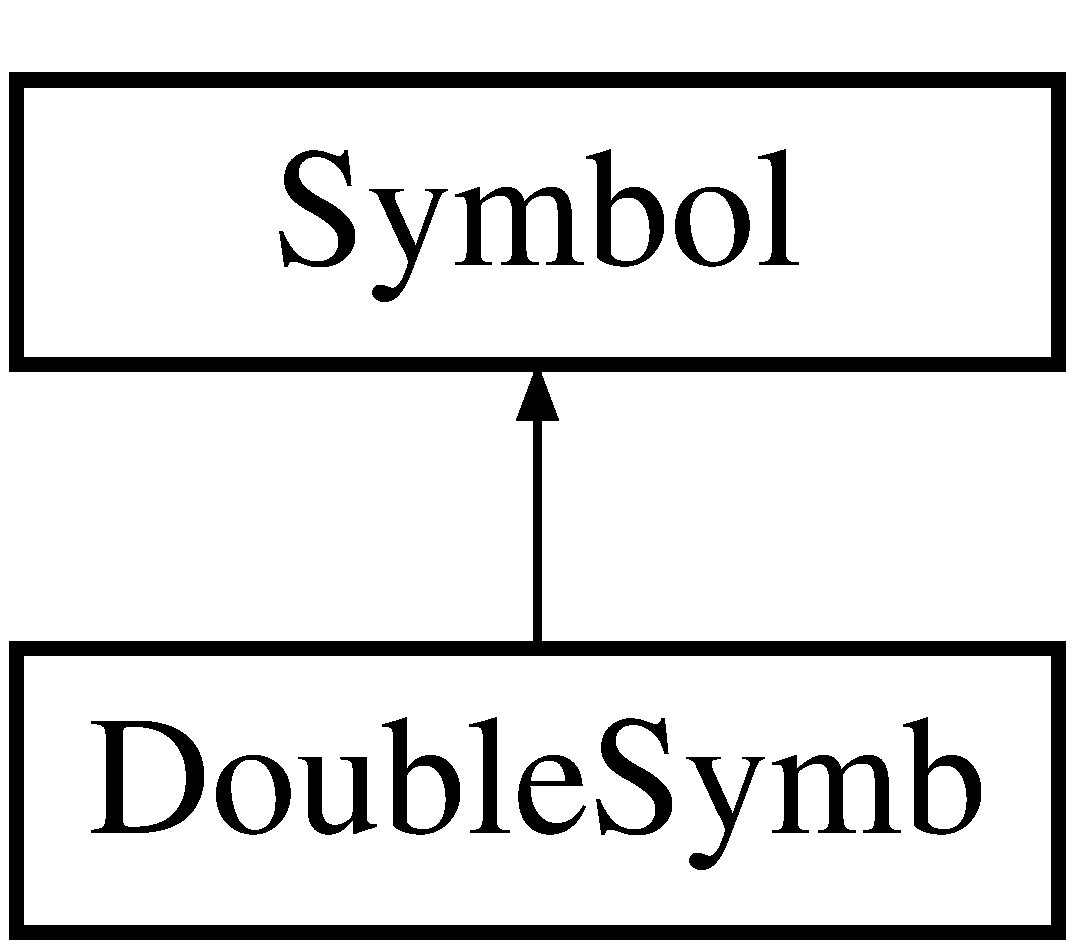
\includegraphics[height=2.000000cm]{class_double_symb}
\end{center}
\end{figure}
\subsection*{Public Member Functions}
\begin{DoxyCompactItemize}
\item 
\hyperlink{class_double_symb_aa338df568f038fb85fbdeefe33488ffd}{Double\+Symb} ()
\item 
\hyperlink{class_double_symb_ae7cb2e3ecc7bac207a9dba3ae0886317}{Double\+Symb} (\hyperlink{class_double_symb}{Double\+Symb} const \&copy)
\item 
\hyperlink{class_double_symb_a67806283db4e2c356654ceef7a91afcb}{Double\+Symb} (double in\+Value)
\item 
virtual std\+::stringstream \hyperlink{class_double_symb_a6bb7ecda5dfda94ecb658733eafc2f38}{print} ()
\item 
virtual \hyperlink{class_symbol}{Symbol} $\ast$ \hyperlink{class_double_symb_a1d8cca63cce9963b43030891f1ff5e48}{add} (\hyperlink{class_symbol}{Symbol} $\ast$operand)
\item 
virtual \hyperlink{class_symbol}{Symbol} $\ast$ \hyperlink{class_double_symb_a0c08d8436a47c3d9e96d19aa80a2bab9}{sub} (\hyperlink{class_symbol}{Symbol} $\ast$operand)
\item 
virtual \hyperlink{class_symbol}{Symbol} $\ast$ \hyperlink{class_double_symb_a7b297714a165576a11ab7ba6b8990f0a}{mult} (\hyperlink{class_symbol}{Symbol} $\ast$operand)
\item 
virtual \hyperlink{class_symbol}{Symbol} $\ast$ \hyperlink{class_double_symb_a3b632822ad185fce623724148c914b8c}{exp} (int exp)
\item 
virtual \hyperlink{class_double_symb}{Double\+Symb} $\ast$ \hyperlink{class_double_symb_a36170febbfcd8709841050db05e6415b}{neg} ()
\item 
virtual \hyperlink{class_double_symb}{Double\+Symb} $\ast$ \hyperlink{class_double_symb_a69077ea0fe3ed9eae80e3710e4be84e2}{clone} ()
\item 
double \hyperlink{class_double_symb_a4d28f9c21ace82744a042a02a7b9728c}{get\+Value} ()
\end{DoxyCompactItemize}
\subsection*{Additional Inherited Members}


\subsection{Detailed Description}


Definition at line 18 of file Double\+Symb.\+h.



\subsection{Constructor \& Destructor Documentation}
\hypertarget{class_double_symb_aa338df568f038fb85fbdeefe33488ffd}{\index{Double\+Symb@{Double\+Symb}!Double\+Symb@{Double\+Symb}}
\index{Double\+Symb@{Double\+Symb}!Double\+Symb@{Double\+Symb}}
\subsubsection[{Double\+Symb}]{\setlength{\rightskip}{0pt plus 5cm}Double\+Symb\+::\+Double\+Symb (
\begin{DoxyParamCaption}
{}
\end{DoxyParamCaption}
)\hspace{0.3cm}{\ttfamily [inline]}}}\label{class_double_symb_aa338df568f038fb85fbdeefe33488ffd}


Definition at line 26 of file Double\+Symb.\+h.

\hypertarget{class_double_symb_ae7cb2e3ecc7bac207a9dba3ae0886317}{\index{Double\+Symb@{Double\+Symb}!Double\+Symb@{Double\+Symb}}
\index{Double\+Symb@{Double\+Symb}!Double\+Symb@{Double\+Symb}}
\subsubsection[{Double\+Symb}]{\setlength{\rightskip}{0pt plus 5cm}Double\+Symb\+::\+Double\+Symb (
\begin{DoxyParamCaption}
\item[{{\bf Double\+Symb} const \&}]{copy}
\end{DoxyParamCaption}
)\hspace{0.3cm}{\ttfamily [inline]}}}\label{class_double_symb_ae7cb2e3ecc7bac207a9dba3ae0886317}


Definition at line 27 of file Double\+Symb.\+h.

\hypertarget{class_double_symb_a67806283db4e2c356654ceef7a91afcb}{\index{Double\+Symb@{Double\+Symb}!Double\+Symb@{Double\+Symb}}
\index{Double\+Symb@{Double\+Symb}!Double\+Symb@{Double\+Symb}}
\subsubsection[{Double\+Symb}]{\setlength{\rightskip}{0pt plus 5cm}Double\+Symb\+::\+Double\+Symb (
\begin{DoxyParamCaption}
\item[{double}]{in\+Value}
\end{DoxyParamCaption}
)\hspace{0.3cm}{\ttfamily [inline]}}}\label{class_double_symb_a67806283db4e2c356654ceef7a91afcb}


Definition at line 28 of file Double\+Symb.\+h.



\subsection{Member Function Documentation}
\hypertarget{class_double_symb_a1d8cca63cce9963b43030891f1ff5e48}{\index{Double\+Symb@{Double\+Symb}!add@{add}}
\index{add@{add}!Double\+Symb@{Double\+Symb}}
\subsubsection[{add}]{\setlength{\rightskip}{0pt plus 5cm}{\bf Symbol} $\ast$ Double\+Symb\+::add (
\begin{DoxyParamCaption}
\item[{{\bf Symbol} $\ast$}]{operand}
\end{DoxyParamCaption}
)\hspace{0.3cm}{\ttfamily [virtual]}}}\label{class_double_symb_a1d8cca63cce9963b43030891f1ff5e48}


Implements \hyperlink{class_symbol_ae8aeeef72df9b6c8f32197e97b909c72}{Symbol}.



Definition at line 17 of file Double\+Symb.\+cpp.

\hypertarget{class_double_symb_a69077ea0fe3ed9eae80e3710e4be84e2}{\index{Double\+Symb@{Double\+Symb}!clone@{clone}}
\index{clone@{clone}!Double\+Symb@{Double\+Symb}}
\subsubsection[{clone}]{\setlength{\rightskip}{0pt plus 5cm}virtual {\bf Double\+Symb}$\ast$ Double\+Symb\+::clone (
\begin{DoxyParamCaption}
{}
\end{DoxyParamCaption}
)\hspace{0.3cm}{\ttfamily [inline]}, {\ttfamily [virtual]}}}\label{class_double_symb_a69077ea0fe3ed9eae80e3710e4be84e2}


Implements \hyperlink{class_symbol_a642df9ea636eb1b7fafa11fc539ea49a}{Symbol}.



Definition at line 37 of file Double\+Symb.\+h.

\hypertarget{class_double_symb_a3b632822ad185fce623724148c914b8c}{\index{Double\+Symb@{Double\+Symb}!exp@{exp}}
\index{exp@{exp}!Double\+Symb@{Double\+Symb}}
\subsubsection[{exp}]{\setlength{\rightskip}{0pt plus 5cm}{\bf Symbol} $\ast$ Double\+Symb\+::exp (
\begin{DoxyParamCaption}
\item[{int}]{exp}
\end{DoxyParamCaption}
)\hspace{0.3cm}{\ttfamily [virtual]}}}\label{class_double_symb_a3b632822ad185fce623724148c914b8c}


Implements \hyperlink{class_symbol_aa259102d6727f267c718b91c78e5eb46}{Symbol}.



Definition at line 116 of file Double\+Symb.\+cpp.

\hypertarget{class_double_symb_a4d28f9c21ace82744a042a02a7b9728c}{\index{Double\+Symb@{Double\+Symb}!get\+Value@{get\+Value}}
\index{get\+Value@{get\+Value}!Double\+Symb@{Double\+Symb}}
\subsubsection[{get\+Value}]{\setlength{\rightskip}{0pt plus 5cm}double Double\+Symb\+::get\+Value (
\begin{DoxyParamCaption}
{}
\end{DoxyParamCaption}
)\hspace{0.3cm}{\ttfamily [inline]}}}\label{class_double_symb_a4d28f9c21ace82744a042a02a7b9728c}


Definition at line 42 of file Double\+Symb.\+h.

\hypertarget{class_double_symb_a7b297714a165576a11ab7ba6b8990f0a}{\index{Double\+Symb@{Double\+Symb}!mult@{mult}}
\index{mult@{mult}!Double\+Symb@{Double\+Symb}}
\subsubsection[{mult}]{\setlength{\rightskip}{0pt plus 5cm}{\bf Symbol} $\ast$ Double\+Symb\+::mult (
\begin{DoxyParamCaption}
\item[{{\bf Symbol} $\ast$}]{operand}
\end{DoxyParamCaption}
)\hspace{0.3cm}{\ttfamily [virtual]}}}\label{class_double_symb_a7b297714a165576a11ab7ba6b8990f0a}


Implements \hyperlink{class_symbol_a224ae5c870650b7704756d8279b9bc53}{Symbol}.



Definition at line 83 of file Double\+Symb.\+cpp.

\hypertarget{class_double_symb_a36170febbfcd8709841050db05e6415b}{\index{Double\+Symb@{Double\+Symb}!neg@{neg}}
\index{neg@{neg}!Double\+Symb@{Double\+Symb}}
\subsubsection[{neg}]{\setlength{\rightskip}{0pt plus 5cm}{\bf Double\+Symb} $\ast$ Double\+Symb\+::neg (
\begin{DoxyParamCaption}
{}
\end{DoxyParamCaption}
)\hspace{0.3cm}{\ttfamily [virtual]}}}\label{class_double_symb_a36170febbfcd8709841050db05e6415b}


Implements \hyperlink{class_symbol_acfc77f36fef51f4d300896d0e5183986}{Symbol}.



Definition at line 125 of file Double\+Symb.\+cpp.

\hypertarget{class_double_symb_a6bb7ecda5dfda94ecb658733eafc2f38}{\index{Double\+Symb@{Double\+Symb}!print@{print}}
\index{print@{print}!Double\+Symb@{Double\+Symb}}
\subsubsection[{print}]{\setlength{\rightskip}{0pt plus 5cm}std\+::stringstream Double\+Symb\+::print (
\begin{DoxyParamCaption}
{}
\end{DoxyParamCaption}
)\hspace{0.3cm}{\ttfamily [virtual]}}}\label{class_double_symb_a6bb7ecda5dfda94ecb658733eafc2f38}


Implements \hyperlink{class_symbol_a327d7b38b13102918bab2a09b8b6a303}{Symbol}.



Definition at line 137 of file Double\+Symb.\+cpp.

\hypertarget{class_double_symb_a0c08d8436a47c3d9e96d19aa80a2bab9}{\index{Double\+Symb@{Double\+Symb}!sub@{sub}}
\index{sub@{sub}!Double\+Symb@{Double\+Symb}}
\subsubsection[{sub}]{\setlength{\rightskip}{0pt plus 5cm}{\bf Symbol} $\ast$ Double\+Symb\+::sub (
\begin{DoxyParamCaption}
\item[{{\bf Symbol} $\ast$}]{operand}
\end{DoxyParamCaption}
)\hspace{0.3cm}{\ttfamily [virtual]}}}\label{class_double_symb_a0c08d8436a47c3d9e96d19aa80a2bab9}


Implements \hyperlink{class_symbol_a53b98ce639c66d1b2e73992f20f56c54}{Symbol}.



Definition at line 49 of file Double\+Symb.\+cpp.



The documentation for this class was generated from the following files\+:\begin{DoxyCompactItemize}
\item 
S\+L\+P/\hyperlink{_double_symb_8h}{Double\+Symb.\+h}\item 
S\+L\+P/\hyperlink{_double_symb_8cpp}{Double\+Symb.\+cpp}\end{DoxyCompactItemize}

\hypertarget{class_exp_op}{\section{Exp\+Op Class Reference}
\label{class_exp_op}\index{Exp\+Op@{Exp\+Op}}
}


{\ttfamily \#include $<$Exp\+Op.\+h$>$}

Inheritance diagram for Exp\+Op\+:\begin{figure}[H]
\begin{center}
\leavevmode
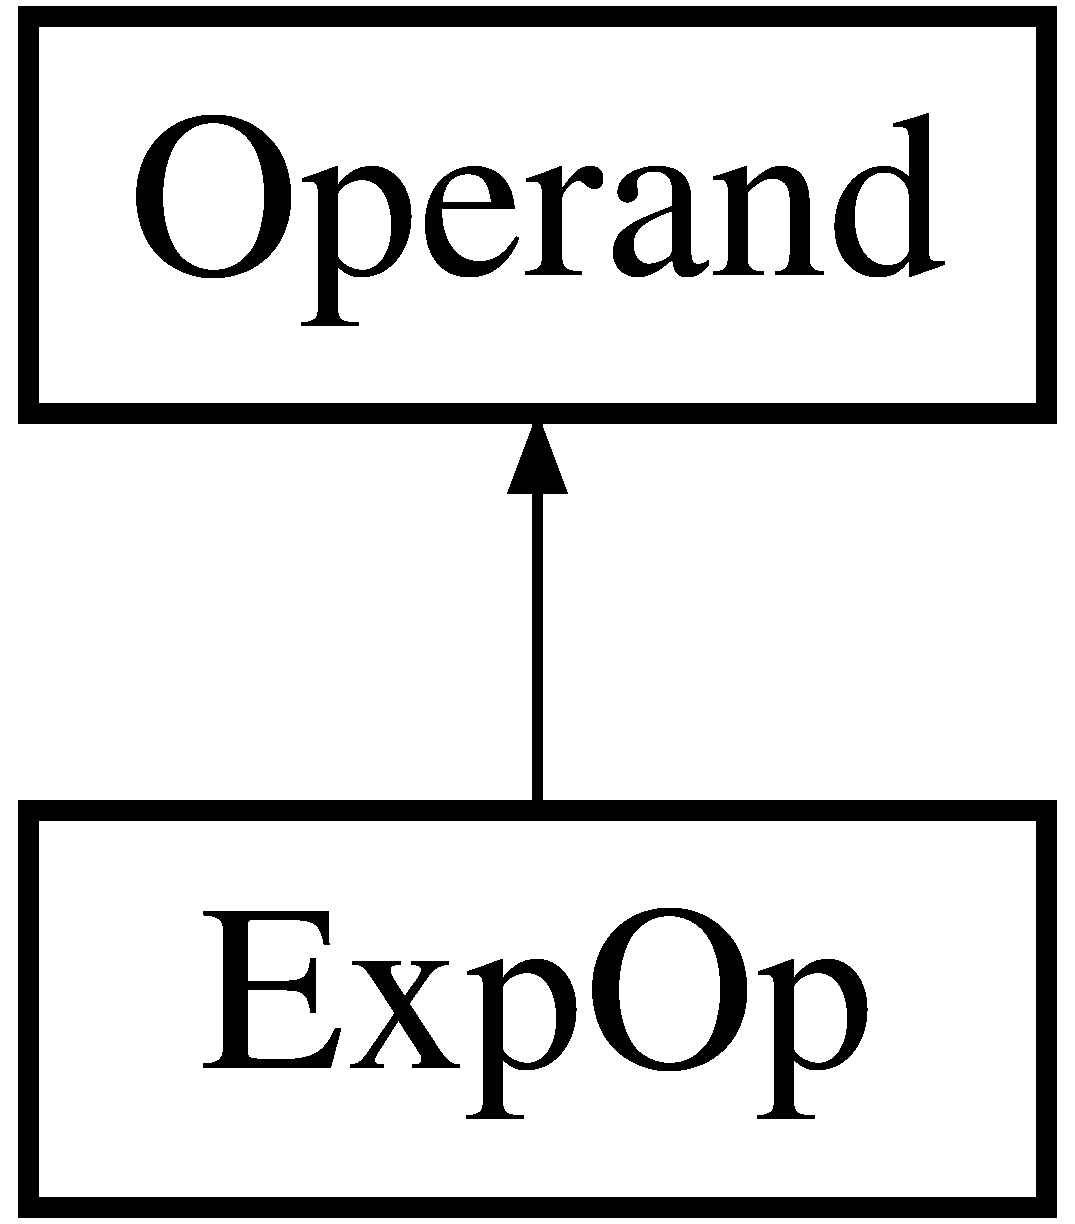
\includegraphics[height=2.000000cm]{class_exp_op}
\end{center}
\end{figure}
\subsection*{Public Member Functions}
\begin{DoxyCompactItemize}
\item 
\hyperlink{class_exp_op_a0541c28e82033972a0b7af563631cf7e}{Exp\+Op} ()
\item 
\hyperlink{class_exp_op_a49862bfd8bd893f648cab4833e941ba7}{Exp\+Op} (\hyperlink{class_operand}{Operand} $\ast$in\+Base, int in\+Exp)
\item 
virtual \hyperlink{class_symbol}{Symbol} $\ast$ \hyperlink{class_exp_op_a56abe7525f95bb5aa6b72ba9d68e56b1}{evaluate} (\hyperlink{class_symbol}{Symbol} $\ast$vars\mbox{[}$\,$\mbox{]})
\item 
virtual std\+::stringstream \hyperlink{class_exp_op_ab983d8c531da78f87e13ee7a57031b36}{print} ()
\item 
virtual \hyperlink{class_operand}{Operand} $\ast$ \hyperlink{class_exp_op_a5f9a55e3ca7ee9369bd41be93e41c2a5}{diff} (int var\+Index)
\item 
virtual void \hyperlink{class_exp_op_aebcfcfed0eb87355cf7bc89ae59bfaa1}{combine\+Adds} ()
\item 
virtual void \hyperlink{class_exp_op_aa17e9aa3c005d1edd0259253521a1e44}{combine\+Mults} ()
\item 
virtual void \hyperlink{class_exp_op_a2262538ea97f669be0e30b023071af77}{clean\+Mults} ()
\item 
virtual void \hyperlink{class_exp_op_a2a7d37dbe75ffbe6559dd3ff30ee89db}{clean\+Adds} ()
\item 
\hyperlink{class_operand}{Operand} $\ast$ \hyperlink{class_exp_op_a7ad9f5fd18040981c46a20e6e9a56d7d}{get\+Base} ()
\item 
int \hyperlink{class_exp_op_a56f4e75e8ea62d89177784c7878f5b44}{get\+Exp} ()
\item 
void \hyperlink{class_exp_op_a74320a1ab14fd2a6a0f093f1a18611a6}{set\+Exp} (int in\+Exp)
\item 
virtual void \hyperlink{class_exp_op_ae7c3e828e61808d41b2087cfeeb4cb28}{add\+Operand} (\hyperlink{class_operand}{Operand} $\ast$op)
\end{DoxyCompactItemize}
\subsection*{Additional Inherited Members}


\subsection{Detailed Description}


Definition at line 18 of file Exp\+Op.\+h.



\subsection{Constructor \& Destructor Documentation}
\hypertarget{class_exp_op_a0541c28e82033972a0b7af563631cf7e}{\index{Exp\+Op@{Exp\+Op}!Exp\+Op@{Exp\+Op}}
\index{Exp\+Op@{Exp\+Op}!Exp\+Op@{Exp\+Op}}
\subsubsection[{Exp\+Op}]{\setlength{\rightskip}{0pt plus 5cm}Exp\+Op\+::\+Exp\+Op (
\begin{DoxyParamCaption}
{}
\end{DoxyParamCaption}
)\hspace{0.3cm}{\ttfamily [inline]}}}\label{class_exp_op_a0541c28e82033972a0b7af563631cf7e}


Definition at line 24 of file Exp\+Op.\+h.

\hypertarget{class_exp_op_a49862bfd8bd893f648cab4833e941ba7}{\index{Exp\+Op@{Exp\+Op}!Exp\+Op@{Exp\+Op}}
\index{Exp\+Op@{Exp\+Op}!Exp\+Op@{Exp\+Op}}
\subsubsection[{Exp\+Op}]{\setlength{\rightskip}{0pt plus 5cm}Exp\+Op\+::\+Exp\+Op (
\begin{DoxyParamCaption}
\item[{{\bf Operand} $\ast$}]{in\+Base, }
\item[{int}]{in\+Exp}
\end{DoxyParamCaption}
)}}\label{class_exp_op_a49862bfd8bd893f648cab4833e941ba7}


Definition at line 14 of file Exp\+Op.\+cpp.



\subsection{Member Function Documentation}
\hypertarget{class_exp_op_ae7c3e828e61808d41b2087cfeeb4cb28}{\index{Exp\+Op@{Exp\+Op}!add\+Operand@{add\+Operand}}
\index{add\+Operand@{add\+Operand}!Exp\+Op@{Exp\+Op}}
\subsubsection[{add\+Operand}]{\setlength{\rightskip}{0pt plus 5cm}virtual void Exp\+Op\+::add\+Operand (
\begin{DoxyParamCaption}
\item[{{\bf Operand} $\ast$}]{op}
\end{DoxyParamCaption}
)\hspace{0.3cm}{\ttfamily [inline]}, {\ttfamily [virtual]}}}\label{class_exp_op_ae7c3e828e61808d41b2087cfeeb4cb28}


Reimplemented from \hyperlink{class_operand_aa4d004991f0b05b9b6aaa566443f63a6}{Operand}.



Definition at line 40 of file Exp\+Op.\+h.

\hypertarget{class_exp_op_a2a7d37dbe75ffbe6559dd3ff30ee89db}{\index{Exp\+Op@{Exp\+Op}!clean\+Adds@{clean\+Adds}}
\index{clean\+Adds@{clean\+Adds}!Exp\+Op@{Exp\+Op}}
\subsubsection[{clean\+Adds}]{\setlength{\rightskip}{0pt plus 5cm}virtual void Exp\+Op\+::clean\+Adds (
\begin{DoxyParamCaption}
{}
\end{DoxyParamCaption}
)\hspace{0.3cm}{\ttfamily [inline]}, {\ttfamily [virtual]}}}\label{class_exp_op_a2a7d37dbe75ffbe6559dd3ff30ee89db}


Implements \hyperlink{class_operand_adce551c3eaf269ed417647d9365fd8de}{Operand}.



Definition at line 34 of file Exp\+Op.\+h.

\hypertarget{class_exp_op_a2262538ea97f669be0e30b023071af77}{\index{Exp\+Op@{Exp\+Op}!clean\+Mults@{clean\+Mults}}
\index{clean\+Mults@{clean\+Mults}!Exp\+Op@{Exp\+Op}}
\subsubsection[{clean\+Mults}]{\setlength{\rightskip}{0pt plus 5cm}void Exp\+Op\+::clean\+Mults (
\begin{DoxyParamCaption}
{}
\end{DoxyParamCaption}
)\hspace{0.3cm}{\ttfamily [virtual]}}}\label{class_exp_op_a2262538ea97f669be0e30b023071af77}


Implements \hyperlink{class_operand_aca12745fcb2d33fda67568181eb19179}{Operand}.



Definition at line 103 of file Exp\+Op.\+cpp.

\hypertarget{class_exp_op_aebcfcfed0eb87355cf7bc89ae59bfaa1}{\index{Exp\+Op@{Exp\+Op}!combine\+Adds@{combine\+Adds}}
\index{combine\+Adds@{combine\+Adds}!Exp\+Op@{Exp\+Op}}
\subsubsection[{combine\+Adds}]{\setlength{\rightskip}{0pt plus 5cm}virtual void Exp\+Op\+::combine\+Adds (
\begin{DoxyParamCaption}
{}
\end{DoxyParamCaption}
)\hspace{0.3cm}{\ttfamily [inline]}, {\ttfamily [virtual]}}}\label{class_exp_op_aebcfcfed0eb87355cf7bc89ae59bfaa1}


Implements \hyperlink{class_operand_a1650a1adf9ed0d15423c746b6cdcdf2b}{Operand}.



Definition at line 31 of file Exp\+Op.\+h.

\hypertarget{class_exp_op_aa17e9aa3c005d1edd0259253521a1e44}{\index{Exp\+Op@{Exp\+Op}!combine\+Mults@{combine\+Mults}}
\index{combine\+Mults@{combine\+Mults}!Exp\+Op@{Exp\+Op}}
\subsubsection[{combine\+Mults}]{\setlength{\rightskip}{0pt plus 5cm}virtual void Exp\+Op\+::combine\+Mults (
\begin{DoxyParamCaption}
{}
\end{DoxyParamCaption}
)\hspace{0.3cm}{\ttfamily [inline]}, {\ttfamily [virtual]}}}\label{class_exp_op_aa17e9aa3c005d1edd0259253521a1e44}


Implements \hyperlink{class_operand_a82913d427a06d6d3f3832ce9ee0e59ff}{Operand}.



Definition at line 32 of file Exp\+Op.\+h.

\hypertarget{class_exp_op_a5f9a55e3ca7ee9369bd41be93e41c2a5}{\index{Exp\+Op@{Exp\+Op}!diff@{diff}}
\index{diff@{diff}!Exp\+Op@{Exp\+Op}}
\subsubsection[{diff}]{\setlength{\rightskip}{0pt plus 5cm}{\bf Operand} $\ast$ Exp\+Op\+::diff (
\begin{DoxyParamCaption}
\item[{int}]{var\+Index}
\end{DoxyParamCaption}
)\hspace{0.3cm}{\ttfamily [virtual]}}}\label{class_exp_op_a5f9a55e3ca7ee9369bd41be93e41c2a5}


Implements \hyperlink{class_operand_a057d6848e78c2cc4d36a5d57ef68fa61}{Operand}.



Definition at line 65 of file Exp\+Op.\+cpp.

\hypertarget{class_exp_op_a56abe7525f95bb5aa6b72ba9d68e56b1}{\index{Exp\+Op@{Exp\+Op}!evaluate@{evaluate}}
\index{evaluate@{evaluate}!Exp\+Op@{Exp\+Op}}
\subsubsection[{evaluate}]{\setlength{\rightskip}{0pt plus 5cm}{\bf Symbol} $\ast$ Exp\+Op\+::evaluate (
\begin{DoxyParamCaption}
\item[{{\bf Symbol} $\ast$}]{vars\mbox{[}$\,$\mbox{]}}
\end{DoxyParamCaption}
)\hspace{0.3cm}{\ttfamily [virtual]}}}\label{class_exp_op_a56abe7525f95bb5aa6b72ba9d68e56b1}


Implements \hyperlink{class_operand_a910e63f6f002b26dd75deb83af9c69a7}{Operand}.



Definition at line 32 of file Exp\+Op.\+cpp.

\hypertarget{class_exp_op_a7ad9f5fd18040981c46a20e6e9a56d7d}{\index{Exp\+Op@{Exp\+Op}!get\+Base@{get\+Base}}
\index{get\+Base@{get\+Base}!Exp\+Op@{Exp\+Op}}
\subsubsection[{get\+Base}]{\setlength{\rightskip}{0pt plus 5cm}{\bf Operand}$\ast$ Exp\+Op\+::get\+Base (
\begin{DoxyParamCaption}
{}
\end{DoxyParamCaption}
)\hspace{0.3cm}{\ttfamily [inline]}}}\label{class_exp_op_a7ad9f5fd18040981c46a20e6e9a56d7d}


Definition at line 36 of file Exp\+Op.\+h.

\hypertarget{class_exp_op_a56f4e75e8ea62d89177784c7878f5b44}{\index{Exp\+Op@{Exp\+Op}!get\+Exp@{get\+Exp}}
\index{get\+Exp@{get\+Exp}!Exp\+Op@{Exp\+Op}}
\subsubsection[{get\+Exp}]{\setlength{\rightskip}{0pt plus 5cm}int Exp\+Op\+::get\+Exp (
\begin{DoxyParamCaption}
{}
\end{DoxyParamCaption}
)\hspace{0.3cm}{\ttfamily [inline]}}}\label{class_exp_op_a56f4e75e8ea62d89177784c7878f5b44}


Definition at line 37 of file Exp\+Op.\+h.

\hypertarget{class_exp_op_ab983d8c531da78f87e13ee7a57031b36}{\index{Exp\+Op@{Exp\+Op}!print@{print}}
\index{print@{print}!Exp\+Op@{Exp\+Op}}
\subsubsection[{print}]{\setlength{\rightskip}{0pt plus 5cm}std\+::stringstream Exp\+Op\+::print (
\begin{DoxyParamCaption}
{}
\end{DoxyParamCaption}
)\hspace{0.3cm}{\ttfamily [virtual]}}}\label{class_exp_op_ab983d8c531da78f87e13ee7a57031b36}


Implements \hyperlink{class_operand_a8cc045602e1f603a5920249a69abde03}{Operand}.



Definition at line 43 of file Exp\+Op.\+cpp.

\hypertarget{class_exp_op_a74320a1ab14fd2a6a0f093f1a18611a6}{\index{Exp\+Op@{Exp\+Op}!set\+Exp@{set\+Exp}}
\index{set\+Exp@{set\+Exp}!Exp\+Op@{Exp\+Op}}
\subsubsection[{set\+Exp}]{\setlength{\rightskip}{0pt plus 5cm}void Exp\+Op\+::set\+Exp (
\begin{DoxyParamCaption}
\item[{int}]{in\+Exp}
\end{DoxyParamCaption}
)\hspace{0.3cm}{\ttfamily [inline]}}}\label{class_exp_op_a74320a1ab14fd2a6a0f093f1a18611a6}


Definition at line 38 of file Exp\+Op.\+h.



The documentation for this class was generated from the following files\+:\begin{DoxyCompactItemize}
\item 
S\+L\+P/\hyperlink{_exp_op_8h}{Exp\+Op.\+h}\item 
S\+L\+P/\hyperlink{_exp_op_8cpp}{Exp\+Op.\+cpp}\end{DoxyCompactItemize}

\hypertarget{class_factor}{\section{Factor Class Reference}
\label{class_factor}\index{Factor@{Factor}}
}


{\ttfamily \#include $<$Factor.\+h$>$}

\subsection*{Static Public Member Functions}
\begin{DoxyCompactItemize}
\item 
static \hyperlink{class_operand}{Operand} $\ast$ \hyperlink{class_factor_a32b4d25bf955b224966521ab6410b721}{reduce\+Term} (\hyperlink{class_operand}{Operand} $\ast$term, \hyperlink{class_operand}{Operand} $\ast$symb)
\item 
static \hyperlink{class_addition_op}{Addition\+Op} $\ast$ \hyperlink{class_factor_a0c0e7abb73bc3de0b241e3862c6946f0}{factor\+Add} (\hyperlink{class_addition_op}{Addition\+Op} $\ast$node)
\item 
static \hyperlink{class_operand}{Operand} $\ast$ \hyperlink{class_factor_a11a8f832b5675426eb1c99d0d04edf25}{find\+Factor} (\hyperlink{class_addition_op}{Addition\+Op} $\ast$terms)
\item 
static void \hyperlink{class_factor_a9356f713c8e7682079658836020aa53e}{split\+Tree} (\hyperlink{class_addition_op}{Addition\+Op} $\ast$base\+Add, \hyperlink{class_operand}{Operand} $\ast$symb, \hyperlink{class_addition_op}{Addition\+Op} $\ast$\hyperlink{class_factor_a0c0e7abb73bc3de0b241e3862c6946f0}{factor\+Add}, \hyperlink{class_addition_op}{Addition\+Op} $\ast$rest\+Add)
\item 
static int \hyperlink{class_factor_ac96af46d1a23f2149d57ffc7b6d4527d}{count\+Adds} (\hyperlink{class_operand}{Operand} $\ast$node)
\item 
static int \hyperlink{class_factor_a46b96eb50bd24d7eb6552472c0900066}{count\+Mults} (\hyperlink{class_operand}{Operand} $\ast$node)
\end{DoxyCompactItemize}
\subsection*{Static Public Attributes}
\begin{DoxyCompactItemize}
\item 
static \hyperlink{class_operand}{Operand} $\ast$ \hyperlink{class_factor_ab9b06006dd838e95ac84c49ba6ae93bb}{test\+Factor} = 0
\end{DoxyCompactItemize}


\subsection{Detailed Description}


Definition at line 32 of file Factor.\+h.



\subsection{Member Function Documentation}
\hypertarget{class_factor_ac96af46d1a23f2149d57ffc7b6d4527d}{\index{Factor@{Factor}!count\+Adds@{count\+Adds}}
\index{count\+Adds@{count\+Adds}!Factor@{Factor}}
\subsubsection[{count\+Adds}]{\setlength{\rightskip}{0pt plus 5cm}int Factor\+::count\+Adds (
\begin{DoxyParamCaption}
\item[{{\bf Operand} $\ast$}]{node}
\end{DoxyParamCaption}
)\hspace{0.3cm}{\ttfamily [static]}}}\label{class_factor_ac96af46d1a23f2149d57ffc7b6d4527d}


Definition at line 561 of file Factor.\+cpp.

\hypertarget{class_factor_a46b96eb50bd24d7eb6552472c0900066}{\index{Factor@{Factor}!count\+Mults@{count\+Mults}}
\index{count\+Mults@{count\+Mults}!Factor@{Factor}}
\subsubsection[{count\+Mults}]{\setlength{\rightskip}{0pt plus 5cm}int Factor\+::count\+Mults (
\begin{DoxyParamCaption}
\item[{{\bf Operand} $\ast$}]{node}
\end{DoxyParamCaption}
)\hspace{0.3cm}{\ttfamily [static]}}}\label{class_factor_a46b96eb50bd24d7eb6552472c0900066}


Definition at line 607 of file Factor.\+cpp.

\hypertarget{class_factor_a0c0e7abb73bc3de0b241e3862c6946f0}{\index{Factor@{Factor}!factor\+Add@{factor\+Add}}
\index{factor\+Add@{factor\+Add}!Factor@{Factor}}
\subsubsection[{factor\+Add}]{\setlength{\rightskip}{0pt plus 5cm}{\bf Addition\+Op} $\ast$ Factor\+::factor\+Add (
\begin{DoxyParamCaption}
\item[{{\bf Addition\+Op} $\ast$}]{node}
\end{DoxyParamCaption}
)\hspace{0.3cm}{\ttfamily [static]}}}\label{class_factor_a0c0e7abb73bc3de0b241e3862c6946f0}


Definition at line 297 of file Factor.\+cpp.

\hypertarget{class_factor_a11a8f832b5675426eb1c99d0d04edf25}{\index{Factor@{Factor}!find\+Factor@{find\+Factor}}
\index{find\+Factor@{find\+Factor}!Factor@{Factor}}
\subsubsection[{find\+Factor}]{\setlength{\rightskip}{0pt plus 5cm}{\bf Operand} $\ast$ Factor\+::find\+Factor (
\begin{DoxyParamCaption}
\item[{{\bf Addition\+Op} $\ast$}]{terms}
\end{DoxyParamCaption}
)\hspace{0.3cm}{\ttfamily [static]}}}\label{class_factor_a11a8f832b5675426eb1c99d0d04edf25}


Definition at line 347 of file Factor.\+cpp.

\hypertarget{class_factor_a32b4d25bf955b224966521ab6410b721}{\index{Factor@{Factor}!reduce\+Term@{reduce\+Term}}
\index{reduce\+Term@{reduce\+Term}!Factor@{Factor}}
\subsubsection[{reduce\+Term}]{\setlength{\rightskip}{0pt plus 5cm}{\bf Operand} $\ast$ Factor\+::reduce\+Term (
\begin{DoxyParamCaption}
\item[{{\bf Operand} $\ast$}]{term, }
\item[{{\bf Operand} $\ast$}]{symb}
\end{DoxyParamCaption}
)\hspace{0.3cm}{\ttfamily [static]}}}\label{class_factor_a32b4d25bf955b224966521ab6410b721}


Definition at line 467 of file Factor.\+cpp.

\hypertarget{class_factor_a9356f713c8e7682079658836020aa53e}{\index{Factor@{Factor}!split\+Tree@{split\+Tree}}
\index{split\+Tree@{split\+Tree}!Factor@{Factor}}
\subsubsection[{split\+Tree}]{\setlength{\rightskip}{0pt plus 5cm}void Factor\+::split\+Tree (
\begin{DoxyParamCaption}
\item[{{\bf Addition\+Op} $\ast$}]{base\+Add, }
\item[{{\bf Operand} $\ast$}]{symb, }
\item[{{\bf Addition\+Op} $\ast$}]{factor\+Add, }
\item[{{\bf Addition\+Op} $\ast$}]{rest\+Add}
\end{DoxyParamCaption}
)\hspace{0.3cm}{\ttfamily [static]}}}\label{class_factor_a9356f713c8e7682079658836020aa53e}


Definition at line 427 of file Factor.\+cpp.



\subsection{Member Data Documentation}
\hypertarget{class_factor_ab9b06006dd838e95ac84c49ba6ae93bb}{\index{Factor@{Factor}!test\+Factor@{test\+Factor}}
\index{test\+Factor@{test\+Factor}!Factor@{Factor}}
\subsubsection[{test\+Factor}]{\setlength{\rightskip}{0pt plus 5cm}{\bf Operand} $\ast$ Factor\+::test\+Factor = 0\hspace{0.3cm}{\ttfamily [static]}}}\label{class_factor_ab9b06006dd838e95ac84c49ba6ae93bb}


Definition at line 73 of file Factor.\+h.



The documentation for this class was generated from the following files\+:\begin{DoxyCompactItemize}
\item 
S\+L\+P/\hyperlink{_factor_8h}{Factor.\+h}\item 
S\+L\+P/\hyperlink{_factor_8cpp}{Factor.\+cpp}\end{DoxyCompactItemize}

\hypertarget{class_int_symb}{\section{Int\+Symb Class Reference}
\label{class_int_symb}\index{Int\+Symb@{Int\+Symb}}
}


{\ttfamily \#include $<$Int\+Symb.\+h$>$}

Inheritance diagram for Int\+Symb\+:\begin{figure}[H]
\begin{center}
\leavevmode
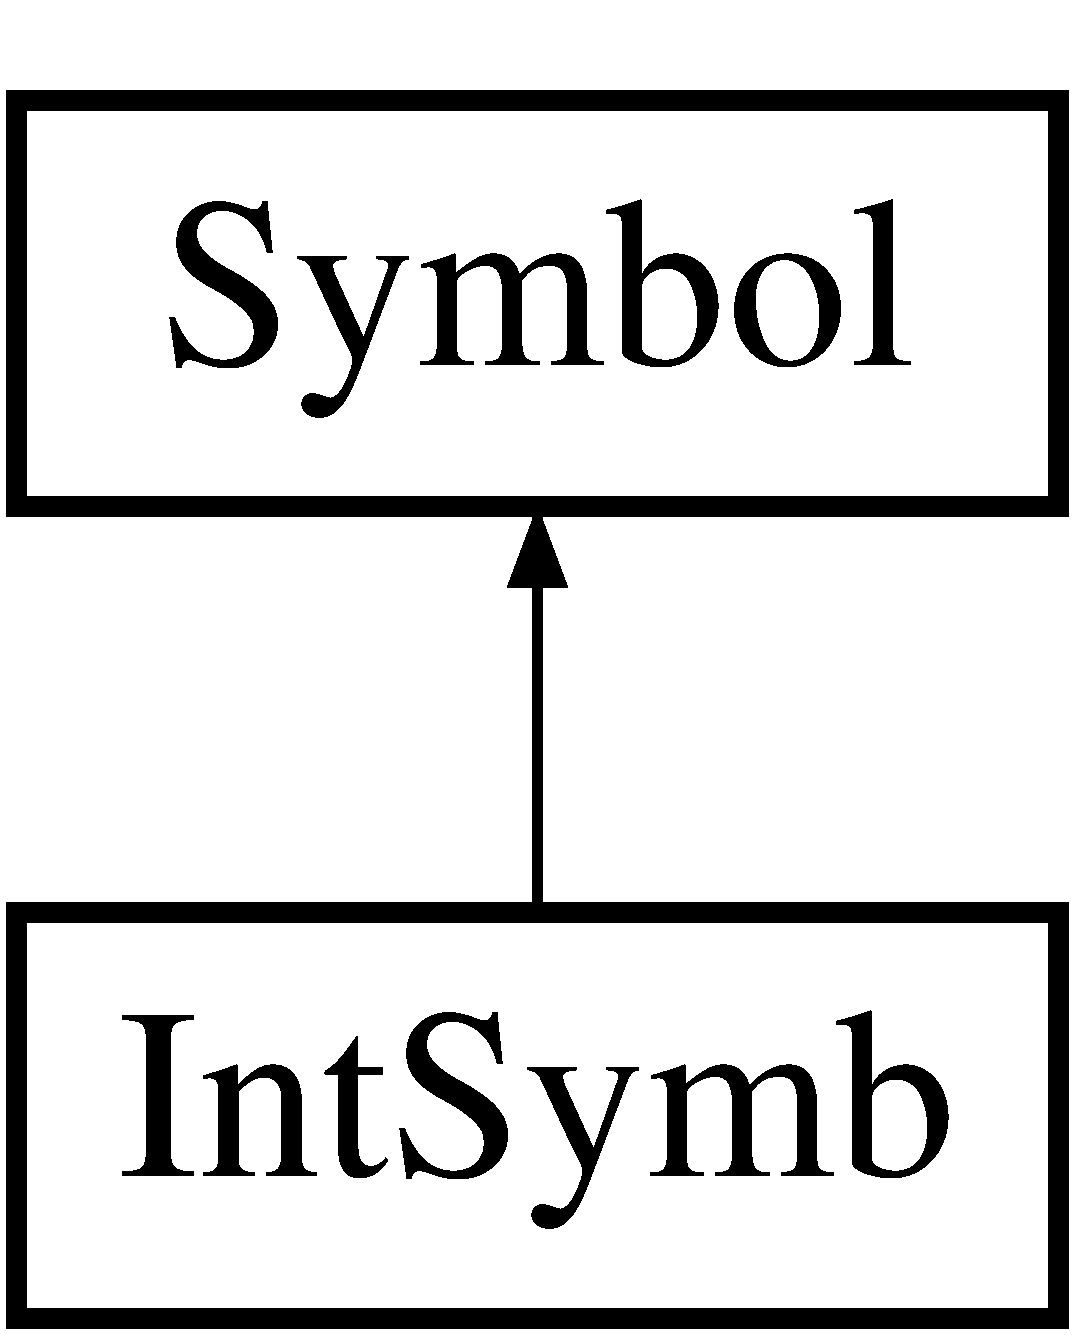
\includegraphics[height=2.000000cm]{class_int_symb}
\end{center}
\end{figure}
\subsection*{Public Member Functions}
\begin{DoxyCompactItemize}
\item 
\hyperlink{class_int_symb_ab3990513e9be8549645e5b6cef5bb8ef}{Int\+Symb} ()
\item 
\hyperlink{class_int_symb_acf0f67c2d4cdd579e1b35d558620faaa}{Int\+Symb} (\hyperlink{class_int_symb}{Int\+Symb} const \&copy)
\item 
\hyperlink{class_int_symb_a45cd842eea27be9fc89adc788c9a6985}{Int\+Symb} (int in\+Value)
\item 
virtual std\+::stringstream \hyperlink{class_int_symb_a22115e6d6a513977d4cdad1013cdd15d}{print} ()
\item 
virtual \hyperlink{class_symbol}{Symbol} $\ast$ \hyperlink{class_int_symb_a10885d3759e4a6765e8d564da4b53b2e}{add} (\hyperlink{class_symbol}{Symbol} $\ast$operand)
\item 
virtual \hyperlink{class_symbol}{Symbol} $\ast$ \hyperlink{class_int_symb_ad4dd7298bf4a8ea002e86671a96f77d9}{sub} (\hyperlink{class_symbol}{Symbol} $\ast$operand)
\item 
virtual \hyperlink{class_symbol}{Symbol} $\ast$ \hyperlink{class_int_symb_ad0b2bd020dfd9c924cac7f722e8aac7e}{mult} (\hyperlink{class_symbol}{Symbol} $\ast$operand)
\item 
virtual \hyperlink{class_int_symb}{Int\+Symb} $\ast$ \hyperlink{class_int_symb_a39254e07e5adc1b4179a39dd8aed49f7}{exp} (int exp)
\item 
virtual \hyperlink{class_int_symb}{Int\+Symb} $\ast$ \hyperlink{class_int_symb_a24d2b18787ec241f268f3e8c259e6e64}{neg} ()
\item 
\hyperlink{class_int_symb}{Int\+Symb} $\ast$ \hyperlink{class_int_symb_a9a57c73450f2a93ca5ff93b0ad8f8aa9}{clone} ()
\item 
int \hyperlink{class_int_symb_acbf0d31076f6adcc3fad9a9bc57c2b82}{get\+Value} ()
\end{DoxyCompactItemize}
\subsection*{Additional Inherited Members}


\subsection{Detailed Description}


Definition at line 17 of file Int\+Symb.\+h.



\subsection{Constructor \& Destructor Documentation}
\hypertarget{class_int_symb_ab3990513e9be8549645e5b6cef5bb8ef}{\index{Int\+Symb@{Int\+Symb}!Int\+Symb@{Int\+Symb}}
\index{Int\+Symb@{Int\+Symb}!Int\+Symb@{Int\+Symb}}
\subsubsection[{Int\+Symb}]{\setlength{\rightskip}{0pt plus 5cm}Int\+Symb\+::\+Int\+Symb (
\begin{DoxyParamCaption}
{}
\end{DoxyParamCaption}
)\hspace{0.3cm}{\ttfamily [inline]}}}\label{class_int_symb_ab3990513e9be8549645e5b6cef5bb8ef}


Definition at line 25 of file Int\+Symb.\+h.

\hypertarget{class_int_symb_acf0f67c2d4cdd579e1b35d558620faaa}{\index{Int\+Symb@{Int\+Symb}!Int\+Symb@{Int\+Symb}}
\index{Int\+Symb@{Int\+Symb}!Int\+Symb@{Int\+Symb}}
\subsubsection[{Int\+Symb}]{\setlength{\rightskip}{0pt plus 5cm}Int\+Symb\+::\+Int\+Symb (
\begin{DoxyParamCaption}
\item[{{\bf Int\+Symb} const \&}]{copy}
\end{DoxyParamCaption}
)\hspace{0.3cm}{\ttfamily [inline]}}}\label{class_int_symb_acf0f67c2d4cdd579e1b35d558620faaa}


Definition at line 26 of file Int\+Symb.\+h.

\hypertarget{class_int_symb_a45cd842eea27be9fc89adc788c9a6985}{\index{Int\+Symb@{Int\+Symb}!Int\+Symb@{Int\+Symb}}
\index{Int\+Symb@{Int\+Symb}!Int\+Symb@{Int\+Symb}}
\subsubsection[{Int\+Symb}]{\setlength{\rightskip}{0pt plus 5cm}Int\+Symb\+::\+Int\+Symb (
\begin{DoxyParamCaption}
\item[{int}]{in\+Value}
\end{DoxyParamCaption}
)\hspace{0.3cm}{\ttfamily [inline]}}}\label{class_int_symb_a45cd842eea27be9fc89adc788c9a6985}


Definition at line 27 of file Int\+Symb.\+h.



\subsection{Member Function Documentation}
\hypertarget{class_int_symb_a10885d3759e4a6765e8d564da4b53b2e}{\index{Int\+Symb@{Int\+Symb}!add@{add}}
\index{add@{add}!Int\+Symb@{Int\+Symb}}
\subsubsection[{add}]{\setlength{\rightskip}{0pt plus 5cm}{\bf Symbol} $\ast$ Int\+Symb\+::add (
\begin{DoxyParamCaption}
\item[{{\bf Symbol} $\ast$}]{operand}
\end{DoxyParamCaption}
)\hspace{0.3cm}{\ttfamily [virtual]}}}\label{class_int_symb_a10885d3759e4a6765e8d564da4b53b2e}


Implements \hyperlink{class_symbol_ae8aeeef72df9b6c8f32197e97b909c72}{Symbol}.



Definition at line 12 of file Int\+Symb.\+cpp.

\hypertarget{class_int_symb_a9a57c73450f2a93ca5ff93b0ad8f8aa9}{\index{Int\+Symb@{Int\+Symb}!clone@{clone}}
\index{clone@{clone}!Int\+Symb@{Int\+Symb}}
\subsubsection[{clone}]{\setlength{\rightskip}{0pt plus 5cm}{\bf Int\+Symb}$\ast$ Int\+Symb\+::clone (
\begin{DoxyParamCaption}
{}
\end{DoxyParamCaption}
)\hspace{0.3cm}{\ttfamily [inline]}, {\ttfamily [virtual]}}}\label{class_int_symb_a9a57c73450f2a93ca5ff93b0ad8f8aa9}


Implements \hyperlink{class_symbol_a642df9ea636eb1b7fafa11fc539ea49a}{Symbol}.



Definition at line 36 of file Int\+Symb.\+h.

\hypertarget{class_int_symb_a39254e07e5adc1b4179a39dd8aed49f7}{\index{Int\+Symb@{Int\+Symb}!exp@{exp}}
\index{exp@{exp}!Int\+Symb@{Int\+Symb}}
\subsubsection[{exp}]{\setlength{\rightskip}{0pt plus 5cm}{\bf Int\+Symb} $\ast$ Int\+Symb\+::exp (
\begin{DoxyParamCaption}
\item[{int}]{exp}
\end{DoxyParamCaption}
)\hspace{0.3cm}{\ttfamily [virtual]}}}\label{class_int_symb_a39254e07e5adc1b4179a39dd8aed49f7}


Implements \hyperlink{class_symbol_aa259102d6727f267c718b91c78e5eb46}{Symbol}.



Definition at line 114 of file Int\+Symb.\+cpp.

\hypertarget{class_int_symb_acbf0d31076f6adcc3fad9a9bc57c2b82}{\index{Int\+Symb@{Int\+Symb}!get\+Value@{get\+Value}}
\index{get\+Value@{get\+Value}!Int\+Symb@{Int\+Symb}}
\subsubsection[{get\+Value}]{\setlength{\rightskip}{0pt plus 5cm}int Int\+Symb\+::get\+Value (
\begin{DoxyParamCaption}
{}
\end{DoxyParamCaption}
)\hspace{0.3cm}{\ttfamily [inline]}}}\label{class_int_symb_acbf0d31076f6adcc3fad9a9bc57c2b82}


Definition at line 41 of file Int\+Symb.\+h.

\hypertarget{class_int_symb_ad0b2bd020dfd9c924cac7f722e8aac7e}{\index{Int\+Symb@{Int\+Symb}!mult@{mult}}
\index{mult@{mult}!Int\+Symb@{Int\+Symb}}
\subsubsection[{mult}]{\setlength{\rightskip}{0pt plus 5cm}{\bf Symbol} $\ast$ Int\+Symb\+::mult (
\begin{DoxyParamCaption}
\item[{{\bf Symbol} $\ast$}]{operand}
\end{DoxyParamCaption}
)\hspace{0.3cm}{\ttfamily [virtual]}}}\label{class_int_symb_ad0b2bd020dfd9c924cac7f722e8aac7e}


Implements \hyperlink{class_symbol_a224ae5c870650b7704756d8279b9bc53}{Symbol}.



Definition at line 82 of file Int\+Symb.\+cpp.

\hypertarget{class_int_symb_a24d2b18787ec241f268f3e8c259e6e64}{\index{Int\+Symb@{Int\+Symb}!neg@{neg}}
\index{neg@{neg}!Int\+Symb@{Int\+Symb}}
\subsubsection[{neg}]{\setlength{\rightskip}{0pt plus 5cm}{\bf Int\+Symb} $\ast$ Int\+Symb\+::neg (
\begin{DoxyParamCaption}
{}
\end{DoxyParamCaption}
)\hspace{0.3cm}{\ttfamily [virtual]}}}\label{class_int_symb_a24d2b18787ec241f268f3e8c259e6e64}


Implements \hyperlink{class_symbol_acfc77f36fef51f4d300896d0e5183986}{Symbol}.



Definition at line 124 of file Int\+Symb.\+cpp.

\hypertarget{class_int_symb_a22115e6d6a513977d4cdad1013cdd15d}{\index{Int\+Symb@{Int\+Symb}!print@{print}}
\index{print@{print}!Int\+Symb@{Int\+Symb}}
\subsubsection[{print}]{\setlength{\rightskip}{0pt plus 5cm}std\+::stringstream Int\+Symb\+::print (
\begin{DoxyParamCaption}
{}
\end{DoxyParamCaption}
)\hspace{0.3cm}{\ttfamily [virtual]}}}\label{class_int_symb_a22115e6d6a513977d4cdad1013cdd15d}


Implements \hyperlink{class_symbol_a327d7b38b13102918bab2a09b8b6a303}{Symbol}.



Definition at line 135 of file Int\+Symb.\+cpp.

\hypertarget{class_int_symb_ad4dd7298bf4a8ea002e86671a96f77d9}{\index{Int\+Symb@{Int\+Symb}!sub@{sub}}
\index{sub@{sub}!Int\+Symb@{Int\+Symb}}
\subsubsection[{sub}]{\setlength{\rightskip}{0pt plus 5cm}{\bf Symbol} $\ast$ Int\+Symb\+::sub (
\begin{DoxyParamCaption}
\item[{{\bf Symbol} $\ast$}]{operand}
\end{DoxyParamCaption}
)\hspace{0.3cm}{\ttfamily [virtual]}}}\label{class_int_symb_ad4dd7298bf4a8ea002e86671a96f77d9}


Implements \hyperlink{class_symbol_a53b98ce639c66d1b2e73992f20f56c54}{Symbol}.



Definition at line 45 of file Int\+Symb.\+cpp.



The documentation for this class was generated from the following files\+:\begin{DoxyCompactItemize}
\item 
S\+L\+P/\hyperlink{_int_symb_8h}{Int\+Symb.\+h}\item 
S\+L\+P/\hyperlink{_int_symb_8cpp}{Int\+Symb.\+cpp}\end{DoxyCompactItemize}

\hypertarget{class_leaf_operand}{\section{Leaf\+Operand Class Reference}
\label{class_leaf_operand}\index{Leaf\+Operand@{Leaf\+Operand}}
}


{\ttfamily \#include $<$Leaf\+Operand.\+h$>$}

Inheritance diagram for Leaf\+Operand\+:\begin{figure}[H]
\begin{center}
\leavevmode
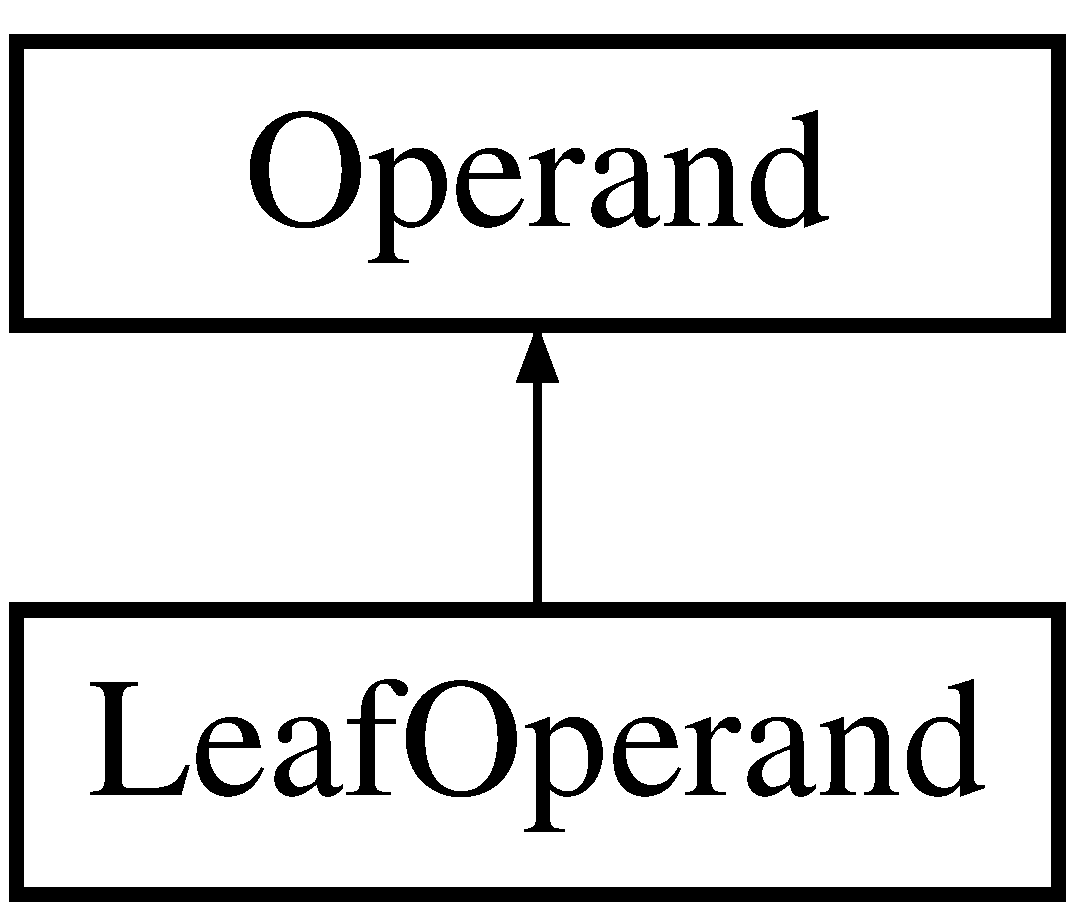
\includegraphics[height=2.000000cm]{class_leaf_operand}
\end{center}
\end{figure}
\subsection*{Public Member Functions}
\begin{DoxyCompactItemize}
\item 
\hyperlink{class_leaf_operand_a82c9cefd1d49381d53b6ea4cf65c314f}{Leaf\+Operand} ()
\item 
\hyperlink{class_leaf_operand_adbe93a55f8afd71db31b6038ef68f6ae}{Leaf\+Operand} (\hyperlink{class_symbol}{Symbol} $\ast$in\+Symb)
\item 
\hyperlink{class_leaf_operand_a6d0a1222d321a82b8b2322e78165c4ba}{Leaf\+Operand} (int index)
\item 
\hyperlink{class_leaf_operand_a33d6c50fa7164efba0bc8aa1b57bf1a0}{Leaf\+Operand} (bool one, bool zero)
\item 
virtual \hyperlink{class_symbol}{Symbol} $\ast$ \hyperlink{class_leaf_operand_ae42e6497dac355f12624a718d6f91a33}{evaluate} (\hyperlink{class_symbol}{Symbol} $\ast$vars\mbox{[}$\,$\mbox{]})
\item 
virtual std\+::stringstream \hyperlink{class_leaf_operand_a3fd735b5d259ad12676f01e84407e0da}{print} ()
\item 
virtual \hyperlink{class_leaf_operand}{Leaf\+Operand} $\ast$ \hyperlink{class_leaf_operand_ada3d818eb13fe43a9117b6140a66072f}{diff} (int invar\+Index)
\item 
virtual void \hyperlink{class_leaf_operand_ae0702803af7b67cf3d1f2da7d27c4698}{combine\+Adds} ()
\item 
virtual void \hyperlink{class_leaf_operand_a11f84bc19234ece8291aaba171692bb8}{combine\+Mults} ()
\item 
virtual void \hyperlink{class_leaf_operand_af5c807f1f53e279f63bd89b89e20272e}{clean\+Mults} ()
\item 
virtual void \hyperlink{class_leaf_operand_ac1f316659c696c5c09fc58a9f02ccc53}{clean\+Adds} ()
\item 
bool \hyperlink{class_leaf_operand_a3674169dd74d3f9f408163f4a796950a}{get\+Is\+Var} ()
\item 
\hyperlink{class_symbol}{Symbol} $\ast$ \hyperlink{class_leaf_operand_aa777cbbfef3b5fcd24622692d7d1821f}{get\+Symb} ()
\item 
bool \hyperlink{class_leaf_operand_aa2b82625a6291864d4afb6f5a1adea15}{get\+Is\+Zero} ()
\item 
bool \hyperlink{class_leaf_operand_a5bc1ec7ac9dbd5f77d598213706fe8e7}{get\+Is\+One} ()
\item 
virtual void \hyperlink{class_leaf_operand_a10d0959f23294fd4929d0b7551168f5c}{add\+Operand} (\hyperlink{class_operand}{Operand} $\ast$op)
\end{DoxyCompactItemize}
\subsection*{Additional Inherited Members}


\subsection{Detailed Description}


Definition at line 17 of file Leaf\+Operand.\+h.



\subsection{Constructor \& Destructor Documentation}
\hypertarget{class_leaf_operand_a82c9cefd1d49381d53b6ea4cf65c314f}{\index{Leaf\+Operand@{Leaf\+Operand}!Leaf\+Operand@{Leaf\+Operand}}
\index{Leaf\+Operand@{Leaf\+Operand}!Leaf\+Operand@{Leaf\+Operand}}
\subsubsection[{Leaf\+Operand}]{\setlength{\rightskip}{0pt plus 5cm}Leaf\+Operand\+::\+Leaf\+Operand (
\begin{DoxyParamCaption}
{}
\end{DoxyParamCaption}
)\hspace{0.3cm}{\ttfamily [inline]}}}\label{class_leaf_operand_a82c9cefd1d49381d53b6ea4cf65c314f}


Definition at line 28 of file Leaf\+Operand.\+h.

\hypertarget{class_leaf_operand_adbe93a55f8afd71db31b6038ef68f6ae}{\index{Leaf\+Operand@{Leaf\+Operand}!Leaf\+Operand@{Leaf\+Operand}}
\index{Leaf\+Operand@{Leaf\+Operand}!Leaf\+Operand@{Leaf\+Operand}}
\subsubsection[{Leaf\+Operand}]{\setlength{\rightskip}{0pt plus 5cm}Leaf\+Operand\+::\+Leaf\+Operand (
\begin{DoxyParamCaption}
\item[{{\bf Symbol} $\ast$}]{in\+Symb}
\end{DoxyParamCaption}
)\hspace{0.3cm}{\ttfamily [inline]}}}\label{class_leaf_operand_adbe93a55f8afd71db31b6038ef68f6ae}


Definition at line 29 of file Leaf\+Operand.\+h.

\hypertarget{class_leaf_operand_a6d0a1222d321a82b8b2322e78165c4ba}{\index{Leaf\+Operand@{Leaf\+Operand}!Leaf\+Operand@{Leaf\+Operand}}
\index{Leaf\+Operand@{Leaf\+Operand}!Leaf\+Operand@{Leaf\+Operand}}
\subsubsection[{Leaf\+Operand}]{\setlength{\rightskip}{0pt plus 5cm}Leaf\+Operand\+::\+Leaf\+Operand (
\begin{DoxyParamCaption}
\item[{int}]{index}
\end{DoxyParamCaption}
)\hspace{0.3cm}{\ttfamily [inline]}}}\label{class_leaf_operand_a6d0a1222d321a82b8b2322e78165c4ba}


Definition at line 30 of file Leaf\+Operand.\+h.

\hypertarget{class_leaf_operand_a33d6c50fa7164efba0bc8aa1b57bf1a0}{\index{Leaf\+Operand@{Leaf\+Operand}!Leaf\+Operand@{Leaf\+Operand}}
\index{Leaf\+Operand@{Leaf\+Operand}!Leaf\+Operand@{Leaf\+Operand}}
\subsubsection[{Leaf\+Operand}]{\setlength{\rightskip}{0pt plus 5cm}Leaf\+Operand\+::\+Leaf\+Operand (
\begin{DoxyParamCaption}
\item[{bool}]{one, }
\item[{bool}]{zero}
\end{DoxyParamCaption}
)\hspace{0.3cm}{\ttfamily [inline]}}}\label{class_leaf_operand_a33d6c50fa7164efba0bc8aa1b57bf1a0}


Definition at line 31 of file Leaf\+Operand.\+h.



\subsection{Member Function Documentation}
\hypertarget{class_leaf_operand_a10d0959f23294fd4929d0b7551168f5c}{\index{Leaf\+Operand@{Leaf\+Operand}!add\+Operand@{add\+Operand}}
\index{add\+Operand@{add\+Operand}!Leaf\+Operand@{Leaf\+Operand}}
\subsubsection[{add\+Operand}]{\setlength{\rightskip}{0pt plus 5cm}virtual void Leaf\+Operand\+::add\+Operand (
\begin{DoxyParamCaption}
\item[{{\bf Operand} $\ast$}]{op}
\end{DoxyParamCaption}
)\hspace{0.3cm}{\ttfamily [inline]}, {\ttfamily [virtual]}}}\label{class_leaf_operand_a10d0959f23294fd4929d0b7551168f5c}


Reimplemented from \hyperlink{class_operand_aa4d004991f0b05b9b6aaa566443f63a6}{Operand}.



Definition at line 56 of file Leaf\+Operand.\+h.

\hypertarget{class_leaf_operand_ac1f316659c696c5c09fc58a9f02ccc53}{\index{Leaf\+Operand@{Leaf\+Operand}!clean\+Adds@{clean\+Adds}}
\index{clean\+Adds@{clean\+Adds}!Leaf\+Operand@{Leaf\+Operand}}
\subsubsection[{clean\+Adds}]{\setlength{\rightskip}{0pt plus 5cm}virtual void Leaf\+Operand\+::clean\+Adds (
\begin{DoxyParamCaption}
{}
\end{DoxyParamCaption}
)\hspace{0.3cm}{\ttfamily [inline]}, {\ttfamily [virtual]}}}\label{class_leaf_operand_ac1f316659c696c5c09fc58a9f02ccc53}


Implements \hyperlink{class_operand_adce551c3eaf269ed417647d9365fd8de}{Operand}.



Definition at line 49 of file Leaf\+Operand.\+h.

\hypertarget{class_leaf_operand_af5c807f1f53e279f63bd89b89e20272e}{\index{Leaf\+Operand@{Leaf\+Operand}!clean\+Mults@{clean\+Mults}}
\index{clean\+Mults@{clean\+Mults}!Leaf\+Operand@{Leaf\+Operand}}
\subsubsection[{clean\+Mults}]{\setlength{\rightskip}{0pt plus 5cm}virtual void Leaf\+Operand\+::clean\+Mults (
\begin{DoxyParamCaption}
{}
\end{DoxyParamCaption}
)\hspace{0.3cm}{\ttfamily [inline]}, {\ttfamily [virtual]}}}\label{class_leaf_operand_af5c807f1f53e279f63bd89b89e20272e}


Implements \hyperlink{class_operand_aca12745fcb2d33fda67568181eb19179}{Operand}.



Definition at line 48 of file Leaf\+Operand.\+h.

\hypertarget{class_leaf_operand_ae0702803af7b67cf3d1f2da7d27c4698}{\index{Leaf\+Operand@{Leaf\+Operand}!combine\+Adds@{combine\+Adds}}
\index{combine\+Adds@{combine\+Adds}!Leaf\+Operand@{Leaf\+Operand}}
\subsubsection[{combine\+Adds}]{\setlength{\rightskip}{0pt plus 5cm}virtual void Leaf\+Operand\+::combine\+Adds (
\begin{DoxyParamCaption}
{}
\end{DoxyParamCaption}
)\hspace{0.3cm}{\ttfamily [inline]}, {\ttfamily [virtual]}}}\label{class_leaf_operand_ae0702803af7b67cf3d1f2da7d27c4698}


Implements \hyperlink{class_operand_a1650a1adf9ed0d15423c746b6cdcdf2b}{Operand}.



Definition at line 46 of file Leaf\+Operand.\+h.

\hypertarget{class_leaf_operand_a11f84bc19234ece8291aaba171692bb8}{\index{Leaf\+Operand@{Leaf\+Operand}!combine\+Mults@{combine\+Mults}}
\index{combine\+Mults@{combine\+Mults}!Leaf\+Operand@{Leaf\+Operand}}
\subsubsection[{combine\+Mults}]{\setlength{\rightskip}{0pt plus 5cm}virtual void Leaf\+Operand\+::combine\+Mults (
\begin{DoxyParamCaption}
{}
\end{DoxyParamCaption}
)\hspace{0.3cm}{\ttfamily [inline]}, {\ttfamily [virtual]}}}\label{class_leaf_operand_a11f84bc19234ece8291aaba171692bb8}


Implements \hyperlink{class_operand_a82913d427a06d6d3f3832ce9ee0e59ff}{Operand}.



Definition at line 47 of file Leaf\+Operand.\+h.

\hypertarget{class_leaf_operand_ada3d818eb13fe43a9117b6140a66072f}{\index{Leaf\+Operand@{Leaf\+Operand}!diff@{diff}}
\index{diff@{diff}!Leaf\+Operand@{Leaf\+Operand}}
\subsubsection[{diff}]{\setlength{\rightskip}{0pt plus 5cm}{\bf Leaf\+Operand} $\ast$ Leaf\+Operand\+::diff (
\begin{DoxyParamCaption}
\item[{int}]{invar\+Index}
\end{DoxyParamCaption}
)\hspace{0.3cm}{\ttfamily [virtual]}}}\label{class_leaf_operand_ada3d818eb13fe43a9117b6140a66072f}


Implements \hyperlink{class_operand_a057d6848e78c2cc4d36a5d57ef68fa61}{Operand}.



Definition at line 89 of file Leaf\+Operand.\+cpp.

\hypertarget{class_leaf_operand_ae42e6497dac355f12624a718d6f91a33}{\index{Leaf\+Operand@{Leaf\+Operand}!evaluate@{evaluate}}
\index{evaluate@{evaluate}!Leaf\+Operand@{Leaf\+Operand}}
\subsubsection[{evaluate}]{\setlength{\rightskip}{0pt plus 5cm}{\bf Symbol} $\ast$ Leaf\+Operand\+::evaluate (
\begin{DoxyParamCaption}
\item[{{\bf Symbol} $\ast$}]{vars\mbox{[}$\,$\mbox{]}}
\end{DoxyParamCaption}
)\hspace{0.3cm}{\ttfamily [virtual]}}}\label{class_leaf_operand_ae42e6497dac355f12624a718d6f91a33}


Implements \hyperlink{class_operand_a910e63f6f002b26dd75deb83af9c69a7}{Operand}.



Definition at line 21 of file Leaf\+Operand.\+cpp.

\hypertarget{class_leaf_operand_a5bc1ec7ac9dbd5f77d598213706fe8e7}{\index{Leaf\+Operand@{Leaf\+Operand}!get\+Is\+One@{get\+Is\+One}}
\index{get\+Is\+One@{get\+Is\+One}!Leaf\+Operand@{Leaf\+Operand}}
\subsubsection[{get\+Is\+One}]{\setlength{\rightskip}{0pt plus 5cm}bool Leaf\+Operand\+::get\+Is\+One (
\begin{DoxyParamCaption}
{}
\end{DoxyParamCaption}
)\hspace{0.3cm}{\ttfamily [inline]}}}\label{class_leaf_operand_a5bc1ec7ac9dbd5f77d598213706fe8e7}


Definition at line 54 of file Leaf\+Operand.\+h.

\hypertarget{class_leaf_operand_a3674169dd74d3f9f408163f4a796950a}{\index{Leaf\+Operand@{Leaf\+Operand}!get\+Is\+Var@{get\+Is\+Var}}
\index{get\+Is\+Var@{get\+Is\+Var}!Leaf\+Operand@{Leaf\+Operand}}
\subsubsection[{get\+Is\+Var}]{\setlength{\rightskip}{0pt plus 5cm}bool Leaf\+Operand\+::get\+Is\+Var (
\begin{DoxyParamCaption}
{}
\end{DoxyParamCaption}
)\hspace{0.3cm}{\ttfamily [inline]}}}\label{class_leaf_operand_a3674169dd74d3f9f408163f4a796950a}


Definition at line 51 of file Leaf\+Operand.\+h.

\hypertarget{class_leaf_operand_aa2b82625a6291864d4afb6f5a1adea15}{\index{Leaf\+Operand@{Leaf\+Operand}!get\+Is\+Zero@{get\+Is\+Zero}}
\index{get\+Is\+Zero@{get\+Is\+Zero}!Leaf\+Operand@{Leaf\+Operand}}
\subsubsection[{get\+Is\+Zero}]{\setlength{\rightskip}{0pt plus 5cm}bool Leaf\+Operand\+::get\+Is\+Zero (
\begin{DoxyParamCaption}
{}
\end{DoxyParamCaption}
)\hspace{0.3cm}{\ttfamily [inline]}}}\label{class_leaf_operand_aa2b82625a6291864d4afb6f5a1adea15}


Definition at line 53 of file Leaf\+Operand.\+h.

\hypertarget{class_leaf_operand_aa777cbbfef3b5fcd24622692d7d1821f}{\index{Leaf\+Operand@{Leaf\+Operand}!get\+Symb@{get\+Symb}}
\index{get\+Symb@{get\+Symb}!Leaf\+Operand@{Leaf\+Operand}}
\subsubsection[{get\+Symb}]{\setlength{\rightskip}{0pt plus 5cm}{\bf Symbol}$\ast$ Leaf\+Operand\+::get\+Symb (
\begin{DoxyParamCaption}
{}
\end{DoxyParamCaption}
)\hspace{0.3cm}{\ttfamily [inline]}}}\label{class_leaf_operand_aa777cbbfef3b5fcd24622692d7d1821f}


Definition at line 52 of file Leaf\+Operand.\+h.

\hypertarget{class_leaf_operand_a3fd735b5d259ad12676f01e84407e0da}{\index{Leaf\+Operand@{Leaf\+Operand}!print@{print}}
\index{print@{print}!Leaf\+Operand@{Leaf\+Operand}}
\subsubsection[{print}]{\setlength{\rightskip}{0pt plus 5cm}std\+::stringstream Leaf\+Operand\+::print (
\begin{DoxyParamCaption}
{}
\end{DoxyParamCaption}
)\hspace{0.3cm}{\ttfamily [virtual]}}}\label{class_leaf_operand_a3fd735b5d259ad12676f01e84407e0da}


Implements \hyperlink{class_operand_a8cc045602e1f603a5920249a69abde03}{Operand}.



Definition at line 55 of file Leaf\+Operand.\+cpp.



The documentation for this class was generated from the following files\+:\begin{DoxyCompactItemize}
\item 
S\+L\+P/\hyperlink{_leaf_operand_8h}{Leaf\+Operand.\+h}\item 
S\+L\+P/\hyperlink{_leaf_operand_8cpp}{Leaf\+Operand.\+cpp}\end{DoxyCompactItemize}

\hypertarget{class_mult_op}{\section{Mult\+Op Class Reference}
\label{class_mult_op}\index{Mult\+Op@{Mult\+Op}}
}


{\ttfamily \#include $<$Mult\+Op.\+h$>$}

Inheritance diagram for Mult\+Op\+:\begin{figure}[H]
\begin{center}
\leavevmode
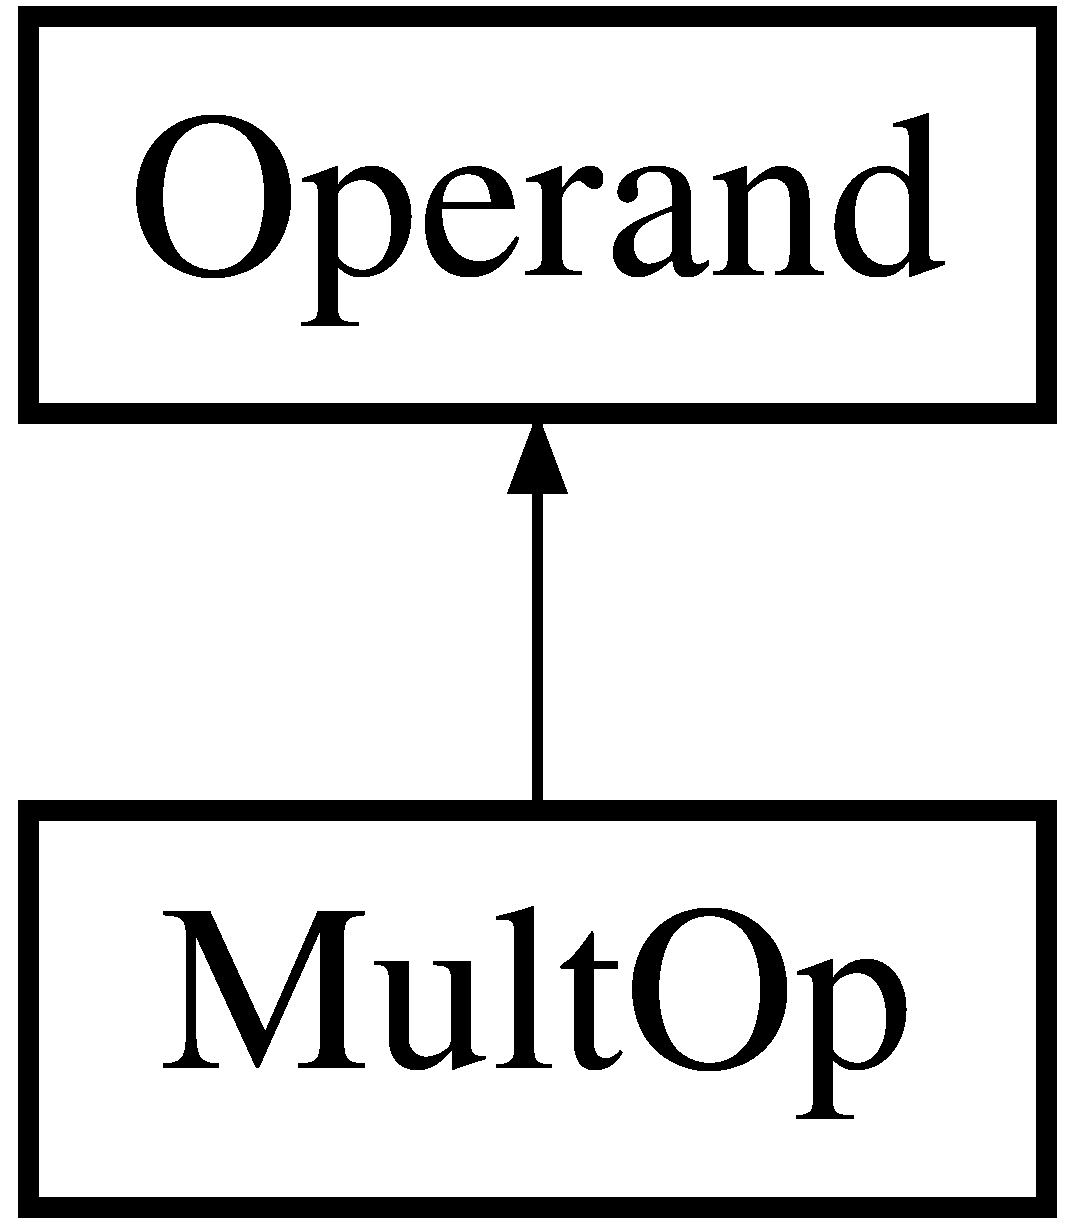
\includegraphics[height=2.000000cm]{class_mult_op}
\end{center}
\end{figure}
\subsection*{Public Member Functions}
\begin{DoxyCompactItemize}
\item 
\hyperlink{class_mult_op_ae0ea2e5997a3cac068c00143680cbb6f}{Mult\+Op} ()
\item 
\hyperlink{class_mult_op_a18a1a7a3d5c65ab3a994d400002610d1}{Mult\+Op} (std\+::vector$<$ \hyperlink{class_operand}{Operand} $\ast$ $>$ in\+Operands)
\item 
virtual \hyperlink{class_symbol}{Symbol} $\ast$ \hyperlink{class_mult_op_ae25e9a6e8e71dab26b15513f8de6a36a}{evaluate} (\hyperlink{class_symbol}{Symbol} $\ast$vars\mbox{[}$\,$\mbox{]})
\item 
virtual std\+::stringstream \hyperlink{class_mult_op_ab08cb5ca6f8ad57596160a98a79f88ae}{print} ()
\item 
virtual \hyperlink{class_addition_op}{Addition\+Op} $\ast$ \hyperlink{class_mult_op_a37b0fd3f963181f326272b7c8de9d86c}{diff} (int var\+Index)
\item 
virtual void \hyperlink{class_mult_op_ae2c71f6cacdf19f30adc3dbb53f54c28}{combine\+Adds} ()
\item 
virtual void \hyperlink{class_mult_op_a53528db5222b6e7d0aa985c0a40e6e6c}{combine\+Mults} ()
\item 
virtual void \hyperlink{class_mult_op_aa46a75fb04c6a595eda8fb3f5d1dc15c}{clean\+Mults} ()
\item 
virtual void \hyperlink{class_mult_op_a84302f5059650d7eb78bb64fe07e4f9d}{clean\+Adds} ()
\end{DoxyCompactItemize}
\subsection*{Additional Inherited Members}


\subsection{Detailed Description}


Definition at line 18 of file Mult\+Op.\+h.



\subsection{Constructor \& Destructor Documentation}
\hypertarget{class_mult_op_ae0ea2e5997a3cac068c00143680cbb6f}{\index{Mult\+Op@{Mult\+Op}!Mult\+Op@{Mult\+Op}}
\index{Mult\+Op@{Mult\+Op}!Mult\+Op@{Mult\+Op}}
\subsubsection[{Mult\+Op}]{\setlength{\rightskip}{0pt plus 5cm}Mult\+Op\+::\+Mult\+Op (
\begin{DoxyParamCaption}
{}
\end{DoxyParamCaption}
)\hspace{0.3cm}{\ttfamily [inline]}}}\label{class_mult_op_ae0ea2e5997a3cac068c00143680cbb6f}


Definition at line 21 of file Mult\+Op.\+h.

\hypertarget{class_mult_op_a18a1a7a3d5c65ab3a994d400002610d1}{\index{Mult\+Op@{Mult\+Op}!Mult\+Op@{Mult\+Op}}
\index{Mult\+Op@{Mult\+Op}!Mult\+Op@{Mult\+Op}}
\subsubsection[{Mult\+Op}]{\setlength{\rightskip}{0pt plus 5cm}Mult\+Op\+::\+Mult\+Op (
\begin{DoxyParamCaption}
\item[{std\+::vector$<$ {\bf Operand} $\ast$ $>$}]{in\+Operands}
\end{DoxyParamCaption}
)}}\label{class_mult_op_a18a1a7a3d5c65ab3a994d400002610d1}


Definition at line 20 of file Mult\+Op.\+cpp.



\subsection{Member Function Documentation}
\hypertarget{class_mult_op_a84302f5059650d7eb78bb64fe07e4f9d}{\index{Mult\+Op@{Mult\+Op}!clean\+Adds@{clean\+Adds}}
\index{clean\+Adds@{clean\+Adds}!Mult\+Op@{Mult\+Op}}
\subsubsection[{clean\+Adds}]{\setlength{\rightskip}{0pt plus 5cm}void Mult\+Op\+::clean\+Adds (
\begin{DoxyParamCaption}
{}
\end{DoxyParamCaption}
)\hspace{0.3cm}{\ttfamily [virtual]}}}\label{class_mult_op_a84302f5059650d7eb78bb64fe07e4f9d}


Implements \hyperlink{class_operand_adce551c3eaf269ed417647d9365fd8de}{Operand}.



Definition at line 383 of file Mult\+Op.\+cpp.

\hypertarget{class_mult_op_aa46a75fb04c6a595eda8fb3f5d1dc15c}{\index{Mult\+Op@{Mult\+Op}!clean\+Mults@{clean\+Mults}}
\index{clean\+Mults@{clean\+Mults}!Mult\+Op@{Mult\+Op}}
\subsubsection[{clean\+Mults}]{\setlength{\rightskip}{0pt plus 5cm}void Mult\+Op\+::clean\+Mults (
\begin{DoxyParamCaption}
{}
\end{DoxyParamCaption}
)\hspace{0.3cm}{\ttfamily [virtual]}}}\label{class_mult_op_aa46a75fb04c6a595eda8fb3f5d1dc15c}


Implements \hyperlink{class_operand_aca12745fcb2d33fda67568181eb19179}{Operand}.



Definition at line 300 of file Mult\+Op.\+cpp.

\hypertarget{class_mult_op_ae2c71f6cacdf19f30adc3dbb53f54c28}{\index{Mult\+Op@{Mult\+Op}!combine\+Adds@{combine\+Adds}}
\index{combine\+Adds@{combine\+Adds}!Mult\+Op@{Mult\+Op}}
\subsubsection[{combine\+Adds}]{\setlength{\rightskip}{0pt plus 5cm}void Mult\+Op\+::combine\+Adds (
\begin{DoxyParamCaption}
{}
\end{DoxyParamCaption}
)\hspace{0.3cm}{\ttfamily [virtual]}}}\label{class_mult_op_ae2c71f6cacdf19f30adc3dbb53f54c28}


Implements \hyperlink{class_operand_a1650a1adf9ed0d15423c746b6cdcdf2b}{Operand}.



Definition at line 195 of file Mult\+Op.\+cpp.

\hypertarget{class_mult_op_a53528db5222b6e7d0aa985c0a40e6e6c}{\index{Mult\+Op@{Mult\+Op}!combine\+Mults@{combine\+Mults}}
\index{combine\+Mults@{combine\+Mults}!Mult\+Op@{Mult\+Op}}
\subsubsection[{combine\+Mults}]{\setlength{\rightskip}{0pt plus 5cm}void Mult\+Op\+::combine\+Mults (
\begin{DoxyParamCaption}
{}
\end{DoxyParamCaption}
)\hspace{0.3cm}{\ttfamily [virtual]}}}\label{class_mult_op_a53528db5222b6e7d0aa985c0a40e6e6c}


Implements \hyperlink{class_operand_a82913d427a06d6d3f3832ce9ee0e59ff}{Operand}.



Definition at line 226 of file Mult\+Op.\+cpp.

\hypertarget{class_mult_op_a37b0fd3f963181f326272b7c8de9d86c}{\index{Mult\+Op@{Mult\+Op}!diff@{diff}}
\index{diff@{diff}!Mult\+Op@{Mult\+Op}}
\subsubsection[{diff}]{\setlength{\rightskip}{0pt plus 5cm}{\bf Addition\+Op} $\ast$ Mult\+Op\+::diff (
\begin{DoxyParamCaption}
\item[{int}]{var\+Index}
\end{DoxyParamCaption}
)\hspace{0.3cm}{\ttfamily [virtual]}}}\label{class_mult_op_a37b0fd3f963181f326272b7c8de9d86c}


Implements \hyperlink{class_operand_a057d6848e78c2cc4d36a5d57ef68fa61}{Operand}.



Definition at line 142 of file Mult\+Op.\+cpp.

\hypertarget{class_mult_op_ae25e9a6e8e71dab26b15513f8de6a36a}{\index{Mult\+Op@{Mult\+Op}!evaluate@{evaluate}}
\index{evaluate@{evaluate}!Mult\+Op@{Mult\+Op}}
\subsubsection[{evaluate}]{\setlength{\rightskip}{0pt plus 5cm}{\bf Symbol} $\ast$ Mult\+Op\+::evaluate (
\begin{DoxyParamCaption}
\item[{{\bf Symbol} $\ast$}]{vars\mbox{[}$\,$\mbox{]}}
\end{DoxyParamCaption}
)\hspace{0.3cm}{\ttfamily [virtual]}}}\label{class_mult_op_ae25e9a6e8e71dab26b15513f8de6a36a}


Implements \hyperlink{class_operand_a910e63f6f002b26dd75deb83af9c69a7}{Operand}.



Definition at line 45 of file Mult\+Op.\+cpp.

\hypertarget{class_mult_op_ab08cb5ca6f8ad57596160a98a79f88ae}{\index{Mult\+Op@{Mult\+Op}!print@{print}}
\index{print@{print}!Mult\+Op@{Mult\+Op}}
\subsubsection[{print}]{\setlength{\rightskip}{0pt plus 5cm}std\+::stringstream Mult\+Op\+::print (
\begin{DoxyParamCaption}
{}
\end{DoxyParamCaption}
)\hspace{0.3cm}{\ttfamily [virtual]}}}\label{class_mult_op_ab08cb5ca6f8ad57596160a98a79f88ae}


Implements \hyperlink{class_operand_a8cc045602e1f603a5920249a69abde03}{Operand}.



Definition at line 83 of file Mult\+Op.\+cpp.



The documentation for this class was generated from the following files\+:\begin{DoxyCompactItemize}
\item 
S\+L\+P/\hyperlink{_mult_op_8h}{Mult\+Op.\+h}\item 
S\+L\+P/\hyperlink{_mult_op_8cpp}{Mult\+Op.\+cpp}\end{DoxyCompactItemize}

\hypertarget{class_operand}{\section{Operand Class Reference}
\label{class_operand}\index{Operand@{Operand}}
}


{\ttfamily \#include $<$Operand.\+h$>$}

Inheritance diagram for Operand\+:\begin{figure}[H]
\begin{center}
\leavevmode
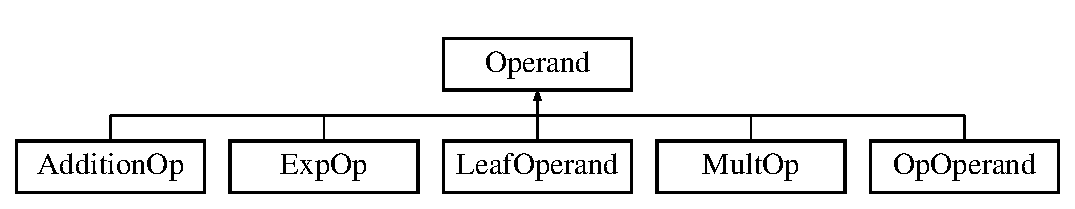
\includegraphics[height=2.000000cm]{class_operand}
\end{center}
\end{figure}
\subsection*{Public Member Functions}
\begin{DoxyCompactItemize}
\item 
virtual \hyperlink{class_symbol}{Symbol} $\ast$ \hyperlink{class_operand_a910e63f6f002b26dd75deb83af9c69a7}{evaluate} (\hyperlink{class_symbol}{Symbol} $\ast$vars\mbox{[}$\,$\mbox{]})=0
\item 
virtual std\+::stringstream \hyperlink{class_operand_a8cc045602e1f603a5920249a69abde03}{print} ()=0
\item 
virtual \hyperlink{class_operand}{Operand} $\ast$ \hyperlink{class_operand_a057d6848e78c2cc4d36a5d57ef68fa61}{diff} (int var\+Index)=0
\item 
virtual void \hyperlink{class_operand_a1650a1adf9ed0d15423c746b6cdcdf2b}{combine\+Adds} ()=0
\item 
virtual void \hyperlink{class_operand_a82913d427a06d6d3f3832ce9ee0e59ff}{combine\+Mults} ()=0
\item 
virtual void \hyperlink{class_operand_aca12745fcb2d33fda67568181eb19179}{clean\+Mults} ()=0
\item 
virtual void \hyperlink{class_operand_adce551c3eaf269ed417647d9365fd8de}{clean\+Adds} ()=0
\item 
int \hyperlink{class_operand_a78a71c37d38e0b703e2f94caa4cfee56}{get\+Type} ()
\item 
virtual std\+::vector$<$ \hyperlink{class_operand}{Operand} $\ast$ $>$ \hyperlink{class_operand_ad51e24642aff7fbeaefebc732bf01565}{get\+Operands} ()
\item 
virtual int \hyperlink{class_operand_ab2648e8880b005d2500d97f583e19022}{get\+Num\+Operands} ()
\item 
virtual void \hyperlink{class_operand_aa4d004991f0b05b9b6aaa566443f63a6}{add\+Operand} (\hyperlink{class_operand}{Operand} $\ast$op)
\item 
void \hyperlink{class_operand_a3ace581e9ed6c16129d30d6862c342e9}{clear} ()
\end{DoxyCompactItemize}
\subsection*{Static Public Member Functions}
\begin{DoxyCompactItemize}
\item 
static void \hyperlink{class_operand_a690d7ad2b55003a28adf37aeaa658527}{clean} (\hyperlink{class_operand}{Operand} $\ast$node)
\end{DoxyCompactItemize}
\subsection*{Static Public Attributes}
\begin{DoxyCompactItemize}
\item 
static const int \hyperlink{class_operand_a72561b58147e35a5a359d9b79118dbb0}{T\+Y\+P\+E\+\_\+\+A\+D\+D} = 1
\item 
static const int \hyperlink{class_operand_a081453264453622326e975742d65bdc8}{T\+Y\+P\+E\+\_\+\+M\+U\+L\+T} = 2
\item 
static const int \hyperlink{class_operand_a16ab8a1b33c8e8a2f576a9027f7f2d21}{T\+Y\+P\+E\+\_\+\+E\+X\+P} = 3
\item 
static const int \hyperlink{class_operand_a9d9c7e7ff88c2ce280aa1332f9b12913}{T\+Y\+P\+E\+\_\+\+L\+E\+A\+F} = 4
\end{DoxyCompactItemize}
\subsection*{Protected Attributes}
\begin{DoxyCompactItemize}
\item 
std\+::vector$<$ \hyperlink{class_operand}{Operand} $\ast$ $>$ \hyperlink{class_operand_a7939bfe67bad92030551774aed8a1b77}{operands}
\item 
int \hyperlink{class_operand_a36baa86e6e7199ef596a647f180a8584}{num\+Operands}
\item 
int \hyperlink{class_operand_a389bb640b257a1fc4ed658a1817591c6}{type}
\end{DoxyCompactItemize}


\subsection{Detailed Description}


Definition at line 30 of file Operand.\+h.



\subsection{Member Function Documentation}
\hypertarget{class_operand_aa4d004991f0b05b9b6aaa566443f63a6}{\index{Operand@{Operand}!add\+Operand@{add\+Operand}}
\index{add\+Operand@{add\+Operand}!Operand@{Operand}}
\subsubsection[{add\+Operand}]{\setlength{\rightskip}{0pt plus 5cm}virtual void Operand\+::add\+Operand (
\begin{DoxyParamCaption}
\item[{{\bf Operand} $\ast$}]{op}
\end{DoxyParamCaption}
)\hspace{0.3cm}{\ttfamily [inline]}, {\ttfamily [virtual]}}}\label{class_operand_aa4d004991f0b05b9b6aaa566443f63a6}


Reimplemented in \hyperlink{class_leaf_operand_a10d0959f23294fd4929d0b7551168f5c}{Leaf\+Operand}, \hyperlink{class_exp_op_ae7c3e828e61808d41b2087cfeeb4cb28}{Exp\+Op}, \hyperlink{class_addition_op_a4a0b8c6e12b6c54857b8b318c6ba55f1}{Addition\+Op}, and \hyperlink{class_op_operand_a97bd0af8d4e30f9815600b26bd0d2349}{Op\+Operand}.



Definition at line 75 of file Operand.\+h.

\hypertarget{class_operand_a690d7ad2b55003a28adf37aeaa658527}{\index{Operand@{Operand}!clean@{clean}}
\index{clean@{clean}!Operand@{Operand}}
\subsubsection[{clean}]{\setlength{\rightskip}{0pt plus 5cm}static void Operand\+::clean (
\begin{DoxyParamCaption}
\item[{{\bf Operand} $\ast$}]{node}
\end{DoxyParamCaption}
)\hspace{0.3cm}{\ttfamily [inline]}, {\ttfamily [static]}}}\label{class_operand_a690d7ad2b55003a28adf37aeaa658527}


Definition at line 65 of file Operand.\+h.

\hypertarget{class_operand_adce551c3eaf269ed417647d9365fd8de}{\index{Operand@{Operand}!clean\+Adds@{clean\+Adds}}
\index{clean\+Adds@{clean\+Adds}!Operand@{Operand}}
\subsubsection[{clean\+Adds}]{\setlength{\rightskip}{0pt plus 5cm}virtual void Operand\+::clean\+Adds (
\begin{DoxyParamCaption}
{}
\end{DoxyParamCaption}
)\hspace{0.3cm}{\ttfamily [pure virtual]}}}\label{class_operand_adce551c3eaf269ed417647d9365fd8de}


Implemented in \hyperlink{class_leaf_operand_ac1f316659c696c5c09fc58a9f02ccc53}{Leaf\+Operand}, \hyperlink{class_exp_op_a2a7d37dbe75ffbe6559dd3ff30ee89db}{Exp\+Op}, \hyperlink{class_addition_op_a4f573734c49e2acff6ae51f15a8698d6}{Addition\+Op}, and \hyperlink{class_mult_op_a84302f5059650d7eb78bb64fe07e4f9d}{Mult\+Op}.

\hypertarget{class_operand_aca12745fcb2d33fda67568181eb19179}{\index{Operand@{Operand}!clean\+Mults@{clean\+Mults}}
\index{clean\+Mults@{clean\+Mults}!Operand@{Operand}}
\subsubsection[{clean\+Mults}]{\setlength{\rightskip}{0pt plus 5cm}virtual void Operand\+::clean\+Mults (
\begin{DoxyParamCaption}
{}
\end{DoxyParamCaption}
)\hspace{0.3cm}{\ttfamily [pure virtual]}}}\label{class_operand_aca12745fcb2d33fda67568181eb19179}


Implemented in \hyperlink{class_leaf_operand_af5c807f1f53e279f63bd89b89e20272e}{Leaf\+Operand}, \hyperlink{class_op_operand_a669d2794a1939e92e976c3ff41e72fc9}{Op\+Operand}, \hyperlink{class_exp_op_a2262538ea97f669be0e30b023071af77}{Exp\+Op}, \hyperlink{class_addition_op_ad04b68e36b5852ec2b951005b71cd56d}{Addition\+Op}, and \hyperlink{class_mult_op_aa46a75fb04c6a595eda8fb3f5d1dc15c}{Mult\+Op}.

\hypertarget{class_operand_a3ace581e9ed6c16129d30d6862c342e9}{\index{Operand@{Operand}!clear@{clear}}
\index{clear@{clear}!Operand@{Operand}}
\subsubsection[{clear}]{\setlength{\rightskip}{0pt plus 5cm}void Operand\+::clear (
\begin{DoxyParamCaption}
{}
\end{DoxyParamCaption}
)\hspace{0.3cm}{\ttfamily [inline]}}}\label{class_operand_a3ace581e9ed6c16129d30d6862c342e9}


Definition at line 76 of file Operand.\+h.

\hypertarget{class_operand_a1650a1adf9ed0d15423c746b6cdcdf2b}{\index{Operand@{Operand}!combine\+Adds@{combine\+Adds}}
\index{combine\+Adds@{combine\+Adds}!Operand@{Operand}}
\subsubsection[{combine\+Adds}]{\setlength{\rightskip}{0pt plus 5cm}virtual void Operand\+::combine\+Adds (
\begin{DoxyParamCaption}
{}
\end{DoxyParamCaption}
)\hspace{0.3cm}{\ttfamily [pure virtual]}}}\label{class_operand_a1650a1adf9ed0d15423c746b6cdcdf2b}


Implemented in \hyperlink{class_leaf_operand_ae0702803af7b67cf3d1f2da7d27c4698}{Leaf\+Operand}, \hyperlink{class_op_operand_a7207c2534050ce2f909e29f4cc3b7345}{Op\+Operand}, \hyperlink{class_exp_op_aebcfcfed0eb87355cf7bc89ae59bfaa1}{Exp\+Op}, \hyperlink{class_addition_op_aae8debc8773974054d3acf6a5df231ff}{Addition\+Op}, and \hyperlink{class_mult_op_ae2c71f6cacdf19f30adc3dbb53f54c28}{Mult\+Op}.

\hypertarget{class_operand_a82913d427a06d6d3f3832ce9ee0e59ff}{\index{Operand@{Operand}!combine\+Mults@{combine\+Mults}}
\index{combine\+Mults@{combine\+Mults}!Operand@{Operand}}
\subsubsection[{combine\+Mults}]{\setlength{\rightskip}{0pt plus 5cm}virtual void Operand\+::combine\+Mults (
\begin{DoxyParamCaption}
{}
\end{DoxyParamCaption}
)\hspace{0.3cm}{\ttfamily [pure virtual]}}}\label{class_operand_a82913d427a06d6d3f3832ce9ee0e59ff}


Implemented in \hyperlink{class_leaf_operand_a11f84bc19234ece8291aaba171692bb8}{Leaf\+Operand}, \hyperlink{class_op_operand_a0e12f3662ac434767c8ad51053870fb2}{Op\+Operand}, \hyperlink{class_exp_op_aa17e9aa3c005d1edd0259253521a1e44}{Exp\+Op}, \hyperlink{class_addition_op_abd35da4badb0e1b02ab271a8f87da472}{Addition\+Op}, and \hyperlink{class_mult_op_a53528db5222b6e7d0aa985c0a40e6e6c}{Mult\+Op}.

\hypertarget{class_operand_a057d6848e78c2cc4d36a5d57ef68fa61}{\index{Operand@{Operand}!diff@{diff}}
\index{diff@{diff}!Operand@{Operand}}
\subsubsection[{diff}]{\setlength{\rightskip}{0pt plus 5cm}virtual {\bf Operand}$\ast$ Operand\+::diff (
\begin{DoxyParamCaption}
\item[{int}]{var\+Index}
\end{DoxyParamCaption}
)\hspace{0.3cm}{\ttfamily [pure virtual]}}}\label{class_operand_a057d6848e78c2cc4d36a5d57ef68fa61}


Implemented in \hyperlink{class_leaf_operand_ada3d818eb13fe43a9117b6140a66072f}{Leaf\+Operand}, \hyperlink{class_exp_op_a5f9a55e3ca7ee9369bd41be93e41c2a5}{Exp\+Op}, \hyperlink{class_addition_op_a0339b4c06997d4592c50f9bf72f578a3}{Addition\+Op}, \hyperlink{class_op_operand_ac20c0b3333ea6f67b677921f561c973b}{Op\+Operand}, and \hyperlink{class_mult_op_a37b0fd3f963181f326272b7c8de9d86c}{Mult\+Op}.

\hypertarget{class_operand_a910e63f6f002b26dd75deb83af9c69a7}{\index{Operand@{Operand}!evaluate@{evaluate}}
\index{evaluate@{evaluate}!Operand@{Operand}}
\subsubsection[{evaluate}]{\setlength{\rightskip}{0pt plus 5cm}virtual {\bf Symbol}$\ast$ Operand\+::evaluate (
\begin{DoxyParamCaption}
\item[{{\bf Symbol} $\ast$}]{vars\mbox{[}$\,$\mbox{]}}
\end{DoxyParamCaption}
)\hspace{0.3cm}{\ttfamily [pure virtual]}}}\label{class_operand_a910e63f6f002b26dd75deb83af9c69a7}


Implemented in \hyperlink{class_leaf_operand_ae42e6497dac355f12624a718d6f91a33}{Leaf\+Operand}, \hyperlink{class_exp_op_a56abe7525f95bb5aa6b72ba9d68e56b1}{Exp\+Op}, \hyperlink{class_addition_op_acc5fa1937f8e82d7e6356d2aa199a5e9}{Addition\+Op}, \hyperlink{class_op_operand_a5c1da397269f8edfb7ebb76c6da16bdb}{Op\+Operand}, and \hyperlink{class_mult_op_ae25e9a6e8e71dab26b15513f8de6a36a}{Mult\+Op}.

\hypertarget{class_operand_ab2648e8880b005d2500d97f583e19022}{\index{Operand@{Operand}!get\+Num\+Operands@{get\+Num\+Operands}}
\index{get\+Num\+Operands@{get\+Num\+Operands}!Operand@{Operand}}
\subsubsection[{get\+Num\+Operands}]{\setlength{\rightskip}{0pt plus 5cm}virtual int Operand\+::get\+Num\+Operands (
\begin{DoxyParamCaption}
{}
\end{DoxyParamCaption}
)\hspace{0.3cm}{\ttfamily [inline]}, {\ttfamily [virtual]}}}\label{class_operand_ab2648e8880b005d2500d97f583e19022}


Reimplemented in \hyperlink{class_op_operand_ab73903f1d3eb535209eb15c992b17c61}{Op\+Operand}.



Definition at line 72 of file Operand.\+h.

\hypertarget{class_operand_ad51e24642aff7fbeaefebc732bf01565}{\index{Operand@{Operand}!get\+Operands@{get\+Operands}}
\index{get\+Operands@{get\+Operands}!Operand@{Operand}}
\subsubsection[{get\+Operands}]{\setlength{\rightskip}{0pt plus 5cm}virtual std\+::vector$<${\bf Operand}$\ast$$>$ Operand\+::get\+Operands (
\begin{DoxyParamCaption}
{}
\end{DoxyParamCaption}
)\hspace{0.3cm}{\ttfamily [inline]}, {\ttfamily [virtual]}}}\label{class_operand_ad51e24642aff7fbeaefebc732bf01565}


Reimplemented in \hyperlink{class_op_operand_a4dabe730f5df82d74919c974fb54e1c6}{Op\+Operand}.



Definition at line 71 of file Operand.\+h.

\hypertarget{class_operand_a78a71c37d38e0b703e2f94caa4cfee56}{\index{Operand@{Operand}!get\+Type@{get\+Type}}
\index{get\+Type@{get\+Type}!Operand@{Operand}}
\subsubsection[{get\+Type}]{\setlength{\rightskip}{0pt plus 5cm}int Operand\+::get\+Type (
\begin{DoxyParamCaption}
{}
\end{DoxyParamCaption}
)\hspace{0.3cm}{\ttfamily [inline]}}}\label{class_operand_a78a71c37d38e0b703e2f94caa4cfee56}


Definition at line 70 of file Operand.\+h.

\hypertarget{class_operand_a8cc045602e1f603a5920249a69abde03}{\index{Operand@{Operand}!print@{print}}
\index{print@{print}!Operand@{Operand}}
\subsubsection[{print}]{\setlength{\rightskip}{0pt plus 5cm}virtual std\+::stringstream Operand\+::print (
\begin{DoxyParamCaption}
{}
\end{DoxyParamCaption}
)\hspace{0.3cm}{\ttfamily [pure virtual]}}}\label{class_operand_a8cc045602e1f603a5920249a69abde03}


Implemented in \hyperlink{class_leaf_operand_a3fd735b5d259ad12676f01e84407e0da}{Leaf\+Operand}, \hyperlink{class_exp_op_ab983d8c531da78f87e13ee7a57031b36}{Exp\+Op}, \hyperlink{class_addition_op_a6e62b558d233e3c358d62e14941872dc}{Addition\+Op}, \hyperlink{class_op_operand_af23227873e50e47d7fa8fb72834d4823}{Op\+Operand}, and \hyperlink{class_mult_op_ab08cb5ca6f8ad57596160a98a79f88ae}{Mult\+Op}.



\subsection{Member Data Documentation}
\hypertarget{class_operand_a36baa86e6e7199ef596a647f180a8584}{\index{Operand@{Operand}!num\+Operands@{num\+Operands}}
\index{num\+Operands@{num\+Operands}!Operand@{Operand}}
\subsubsection[{num\+Operands}]{\setlength{\rightskip}{0pt plus 5cm}int Operand\+::num\+Operands\hspace{0.3cm}{\ttfamily [protected]}}}\label{class_operand_a36baa86e6e7199ef596a647f180a8584}


Definition at line 37 of file Operand.\+h.

\hypertarget{class_operand_a7939bfe67bad92030551774aed8a1b77}{\index{Operand@{Operand}!operands@{operands}}
\index{operands@{operands}!Operand@{Operand}}
\subsubsection[{operands}]{\setlength{\rightskip}{0pt plus 5cm}std\+::vector$<${\bf Operand}$\ast$$>$ Operand\+::operands\hspace{0.3cm}{\ttfamily [protected]}}}\label{class_operand_a7939bfe67bad92030551774aed8a1b77}


Definition at line 35 of file Operand.\+h.

\hypertarget{class_operand_a389bb640b257a1fc4ed658a1817591c6}{\index{Operand@{Operand}!type@{type}}
\index{type@{type}!Operand@{Operand}}
\subsubsection[{type}]{\setlength{\rightskip}{0pt plus 5cm}int Operand\+::type\hspace{0.3cm}{\ttfamily [protected]}}}\label{class_operand_a389bb640b257a1fc4ed658a1817591c6}


Definition at line 40 of file Operand.\+h.

\hypertarget{class_operand_a72561b58147e35a5a359d9b79118dbb0}{\index{Operand@{Operand}!T\+Y\+P\+E\+\_\+\+A\+D\+D@{T\+Y\+P\+E\+\_\+\+A\+D\+D}}
\index{T\+Y\+P\+E\+\_\+\+A\+D\+D@{T\+Y\+P\+E\+\_\+\+A\+D\+D}!Operand@{Operand}}
\subsubsection[{T\+Y\+P\+E\+\_\+\+A\+D\+D}]{\setlength{\rightskip}{0pt plus 5cm}const int Operand\+::\+T\+Y\+P\+E\+\_\+\+A\+D\+D = 1\hspace{0.3cm}{\ttfamily [static]}}}\label{class_operand_a72561b58147e35a5a359d9b79118dbb0}


Definition at line 44 of file Operand.\+h.

\hypertarget{class_operand_a16ab8a1b33c8e8a2f576a9027f7f2d21}{\index{Operand@{Operand}!T\+Y\+P\+E\+\_\+\+E\+X\+P@{T\+Y\+P\+E\+\_\+\+E\+X\+P}}
\index{T\+Y\+P\+E\+\_\+\+E\+X\+P@{T\+Y\+P\+E\+\_\+\+E\+X\+P}!Operand@{Operand}}
\subsubsection[{T\+Y\+P\+E\+\_\+\+E\+X\+P}]{\setlength{\rightskip}{0pt plus 5cm}const int Operand\+::\+T\+Y\+P\+E\+\_\+\+E\+X\+P = 3\hspace{0.3cm}{\ttfamily [static]}}}\label{class_operand_a16ab8a1b33c8e8a2f576a9027f7f2d21}


Definition at line 46 of file Operand.\+h.

\hypertarget{class_operand_a9d9c7e7ff88c2ce280aa1332f9b12913}{\index{Operand@{Operand}!T\+Y\+P\+E\+\_\+\+L\+E\+A\+F@{T\+Y\+P\+E\+\_\+\+L\+E\+A\+F}}
\index{T\+Y\+P\+E\+\_\+\+L\+E\+A\+F@{T\+Y\+P\+E\+\_\+\+L\+E\+A\+F}!Operand@{Operand}}
\subsubsection[{T\+Y\+P\+E\+\_\+\+L\+E\+A\+F}]{\setlength{\rightskip}{0pt plus 5cm}const int Operand\+::\+T\+Y\+P\+E\+\_\+\+L\+E\+A\+F = 4\hspace{0.3cm}{\ttfamily [static]}}}\label{class_operand_a9d9c7e7ff88c2ce280aa1332f9b12913}


Definition at line 47 of file Operand.\+h.

\hypertarget{class_operand_a081453264453622326e975742d65bdc8}{\index{Operand@{Operand}!T\+Y\+P\+E\+\_\+\+M\+U\+L\+T@{T\+Y\+P\+E\+\_\+\+M\+U\+L\+T}}
\index{T\+Y\+P\+E\+\_\+\+M\+U\+L\+T@{T\+Y\+P\+E\+\_\+\+M\+U\+L\+T}!Operand@{Operand}}
\subsubsection[{T\+Y\+P\+E\+\_\+\+M\+U\+L\+T}]{\setlength{\rightskip}{0pt plus 5cm}const int Operand\+::\+T\+Y\+P\+E\+\_\+\+M\+U\+L\+T = 2\hspace{0.3cm}{\ttfamily [static]}}}\label{class_operand_a081453264453622326e975742d65bdc8}


Definition at line 45 of file Operand.\+h.



The documentation for this class was generated from the following file\+:\begin{DoxyCompactItemize}
\item 
S\+L\+P/\hyperlink{_operand_8h}{Operand.\+h}\end{DoxyCompactItemize}

\hypertarget{class_op_operand}{\section{Op\+Operand Class Reference}
\label{class_op_operand}\index{Op\+Operand@{Op\+Operand}}
}


{\ttfamily \#include $<$Op\+Operand.\+h$>$}

Inheritance diagram for Op\+Operand\+:\begin{figure}[H]
\begin{center}
\leavevmode
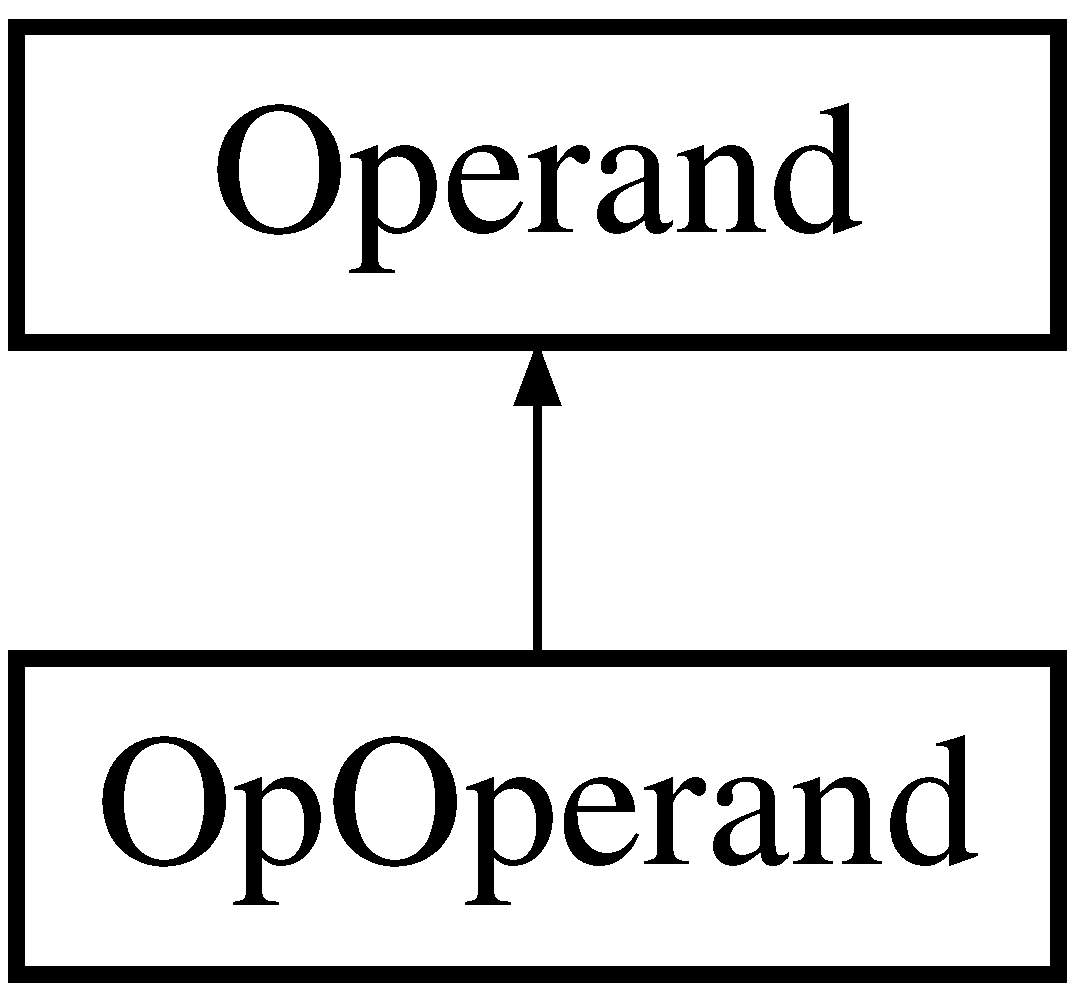
\includegraphics[height=2.000000cm]{class_op_operand}
\end{center}
\end{figure}
\subsection*{Public Member Functions}
\begin{DoxyCompactItemize}
\item 
virtual \hyperlink{class_symbol}{Symbol} $\ast$ \hyperlink{class_op_operand_a5c1da397269f8edfb7ebb76c6da16bdb}{evaluate} (\hyperlink{class_symbol}{Symbol} $\ast$vars\mbox{[}$\,$\mbox{]})=0
\item 
virtual std\+::stringstream \hyperlink{class_op_operand_af23227873e50e47d7fa8fb72834d4823}{print} ()=0
\item 
virtual \hyperlink{class_operand}{Operand} $\ast$ \hyperlink{class_op_operand_ac20c0b3333ea6f67b677921f561c973b}{diff} (int var\+Index)=0
\item 
int \hyperlink{class_op_operand_ab73903f1d3eb535209eb15c992b17c61}{get\+Num\+Operands} ()
\item 
virtual std\+::vector$<$ \hyperlink{class_operand}{Operand} $\ast$ $>$ \hyperlink{class_op_operand_a4dabe730f5df82d74919c974fb54e1c6}{get\+Operands} ()
\item 
virtual void \hyperlink{class_op_operand_a97bd0af8d4e30f9815600b26bd0d2349}{add\+Operand} (\hyperlink{class_operand}{Operand} $\ast$op)
\item 
void \hyperlink{class_op_operand_a074990400d19506a0f82081b99ac5e19}{clear} ()
\item 
virtual void \hyperlink{class_op_operand_a7207c2534050ce2f909e29f4cc3b7345}{combine\+Adds} ()=0
\item 
virtual void \hyperlink{class_op_operand_a0e12f3662ac434767c8ad51053870fb2}{combine\+Mults} ()=0
\item 
virtual void \hyperlink{class_op_operand_a669d2794a1939e92e976c3ff41e72fc9}{clean\+Mults} ()=0
\end{DoxyCompactItemize}
\subsection*{Protected Attributes}
\begin{DoxyCompactItemize}
\item 
std\+::vector$<$ \hyperlink{class_operand}{Operand} $\ast$ $>$ \hyperlink{class_op_operand_a49873cda1ad02191eb14b57a3455f984}{operands}
\item 
int \hyperlink{class_op_operand_a1d559ad86d7efc1db7a6e90788847023}{num\+Operands}
\end{DoxyCompactItemize}
\subsection*{Additional Inherited Members}


\subsection{Detailed Description}


Definition at line 18 of file Op\+Operand.\+h.



\subsection{Member Function Documentation}
\hypertarget{class_op_operand_a97bd0af8d4e30f9815600b26bd0d2349}{\index{Op\+Operand@{Op\+Operand}!add\+Operand@{add\+Operand}}
\index{add\+Operand@{add\+Operand}!Op\+Operand@{Op\+Operand}}
\subsubsection[{add\+Operand}]{\setlength{\rightskip}{0pt plus 5cm}virtual void Op\+Operand\+::add\+Operand (
\begin{DoxyParamCaption}
\item[{{\bf Operand} $\ast$}]{op}
\end{DoxyParamCaption}
)\hspace{0.3cm}{\ttfamily [inline]}, {\ttfamily [virtual]}}}\label{class_op_operand_a97bd0af8d4e30f9815600b26bd0d2349}


Reimplemented from \hyperlink{class_operand_aa4d004991f0b05b9b6aaa566443f63a6}{Operand}.



Definition at line 32 of file Op\+Operand.\+h.

\hypertarget{class_op_operand_a669d2794a1939e92e976c3ff41e72fc9}{\index{Op\+Operand@{Op\+Operand}!clean\+Mults@{clean\+Mults}}
\index{clean\+Mults@{clean\+Mults}!Op\+Operand@{Op\+Operand}}
\subsubsection[{clean\+Mults}]{\setlength{\rightskip}{0pt plus 5cm}virtual void Op\+Operand\+::clean\+Mults (
\begin{DoxyParamCaption}
{}
\end{DoxyParamCaption}
)\hspace{0.3cm}{\ttfamily [pure virtual]}}}\label{class_op_operand_a669d2794a1939e92e976c3ff41e72fc9}


Implements \hyperlink{class_operand_aca12745fcb2d33fda67568181eb19179}{Operand}.

\hypertarget{class_op_operand_a074990400d19506a0f82081b99ac5e19}{\index{Op\+Operand@{Op\+Operand}!clear@{clear}}
\index{clear@{clear}!Op\+Operand@{Op\+Operand}}
\subsubsection[{clear}]{\setlength{\rightskip}{0pt plus 5cm}void Op\+Operand\+::clear (
\begin{DoxyParamCaption}
{}
\end{DoxyParamCaption}
)\hspace{0.3cm}{\ttfamily [inline]}}}\label{class_op_operand_a074990400d19506a0f82081b99ac5e19}


Definition at line 35 of file Op\+Operand.\+h.

\hypertarget{class_op_operand_a7207c2534050ce2f909e29f4cc3b7345}{\index{Op\+Operand@{Op\+Operand}!combine\+Adds@{combine\+Adds}}
\index{combine\+Adds@{combine\+Adds}!Op\+Operand@{Op\+Operand}}
\subsubsection[{combine\+Adds}]{\setlength{\rightskip}{0pt plus 5cm}virtual void Op\+Operand\+::combine\+Adds (
\begin{DoxyParamCaption}
{}
\end{DoxyParamCaption}
)\hspace{0.3cm}{\ttfamily [pure virtual]}}}\label{class_op_operand_a7207c2534050ce2f909e29f4cc3b7345}


Implements \hyperlink{class_operand_a1650a1adf9ed0d15423c746b6cdcdf2b}{Operand}.

\hypertarget{class_op_operand_a0e12f3662ac434767c8ad51053870fb2}{\index{Op\+Operand@{Op\+Operand}!combine\+Mults@{combine\+Mults}}
\index{combine\+Mults@{combine\+Mults}!Op\+Operand@{Op\+Operand}}
\subsubsection[{combine\+Mults}]{\setlength{\rightskip}{0pt plus 5cm}virtual void Op\+Operand\+::combine\+Mults (
\begin{DoxyParamCaption}
{}
\end{DoxyParamCaption}
)\hspace{0.3cm}{\ttfamily [pure virtual]}}}\label{class_op_operand_a0e12f3662ac434767c8ad51053870fb2}


Implements \hyperlink{class_operand_a82913d427a06d6d3f3832ce9ee0e59ff}{Operand}.

\hypertarget{class_op_operand_ac20c0b3333ea6f67b677921f561c973b}{\index{Op\+Operand@{Op\+Operand}!diff@{diff}}
\index{diff@{diff}!Op\+Operand@{Op\+Operand}}
\subsubsection[{diff}]{\setlength{\rightskip}{0pt plus 5cm}virtual {\bf Operand}$\ast$ Op\+Operand\+::diff (
\begin{DoxyParamCaption}
\item[{int}]{var\+Index}
\end{DoxyParamCaption}
)\hspace{0.3cm}{\ttfamily [pure virtual]}}}\label{class_op_operand_ac20c0b3333ea6f67b677921f561c973b}


Implements \hyperlink{class_operand_a057d6848e78c2cc4d36a5d57ef68fa61}{Operand}.

\hypertarget{class_op_operand_a5c1da397269f8edfb7ebb76c6da16bdb}{\index{Op\+Operand@{Op\+Operand}!evaluate@{evaluate}}
\index{evaluate@{evaluate}!Op\+Operand@{Op\+Operand}}
\subsubsection[{evaluate}]{\setlength{\rightskip}{0pt plus 5cm}virtual {\bf Symbol}$\ast$ Op\+Operand\+::evaluate (
\begin{DoxyParamCaption}
\item[{{\bf Symbol} $\ast$}]{vars\mbox{[}$\,$\mbox{]}}
\end{DoxyParamCaption}
)\hspace{0.3cm}{\ttfamily [pure virtual]}}}\label{class_op_operand_a5c1da397269f8edfb7ebb76c6da16bdb}


Implements \hyperlink{class_operand_a910e63f6f002b26dd75deb83af9c69a7}{Operand}.

\hypertarget{class_op_operand_ab73903f1d3eb535209eb15c992b17c61}{\index{Op\+Operand@{Op\+Operand}!get\+Num\+Operands@{get\+Num\+Operands}}
\index{get\+Num\+Operands@{get\+Num\+Operands}!Op\+Operand@{Op\+Operand}}
\subsubsection[{get\+Num\+Operands}]{\setlength{\rightskip}{0pt plus 5cm}int Op\+Operand\+::get\+Num\+Operands (
\begin{DoxyParamCaption}
{}
\end{DoxyParamCaption}
)\hspace{0.3cm}{\ttfamily [inline]}, {\ttfamily [virtual]}}}\label{class_op_operand_ab73903f1d3eb535209eb15c992b17c61}


Reimplemented from \hyperlink{class_operand_ab2648e8880b005d2500d97f583e19022}{Operand}.



Definition at line 29 of file Op\+Operand.\+h.

\hypertarget{class_op_operand_a4dabe730f5df82d74919c974fb54e1c6}{\index{Op\+Operand@{Op\+Operand}!get\+Operands@{get\+Operands}}
\index{get\+Operands@{get\+Operands}!Op\+Operand@{Op\+Operand}}
\subsubsection[{get\+Operands}]{\setlength{\rightskip}{0pt plus 5cm}virtual std\+::vector$<${\bf Operand}$\ast$$>$ Op\+Operand\+::get\+Operands (
\begin{DoxyParamCaption}
{}
\end{DoxyParamCaption}
)\hspace{0.3cm}{\ttfamily [inline]}, {\ttfamily [virtual]}}}\label{class_op_operand_a4dabe730f5df82d74919c974fb54e1c6}


Reimplemented from \hyperlink{class_operand_ad51e24642aff7fbeaefebc732bf01565}{Operand}.



Definition at line 30 of file Op\+Operand.\+h.

\hypertarget{class_op_operand_af23227873e50e47d7fa8fb72834d4823}{\index{Op\+Operand@{Op\+Operand}!print@{print}}
\index{print@{print}!Op\+Operand@{Op\+Operand}}
\subsubsection[{print}]{\setlength{\rightskip}{0pt plus 5cm}virtual std\+::stringstream Op\+Operand\+::print (
\begin{DoxyParamCaption}
{}
\end{DoxyParamCaption}
)\hspace{0.3cm}{\ttfamily [pure virtual]}}}\label{class_op_operand_af23227873e50e47d7fa8fb72834d4823}


Implements \hyperlink{class_operand_a8cc045602e1f603a5920249a69abde03}{Operand}.



\subsection{Member Data Documentation}
\hypertarget{class_op_operand_a1d559ad86d7efc1db7a6e90788847023}{\index{Op\+Operand@{Op\+Operand}!num\+Operands@{num\+Operands}}
\index{num\+Operands@{num\+Operands}!Op\+Operand@{Op\+Operand}}
\subsubsection[{num\+Operands}]{\setlength{\rightskip}{0pt plus 5cm}int Op\+Operand\+::num\+Operands\hspace{0.3cm}{\ttfamily [protected]}}}\label{class_op_operand_a1d559ad86d7efc1db7a6e90788847023}


Definition at line 22 of file Op\+Operand.\+h.

\hypertarget{class_op_operand_a49873cda1ad02191eb14b57a3455f984}{\index{Op\+Operand@{Op\+Operand}!operands@{operands}}
\index{operands@{operands}!Op\+Operand@{Op\+Operand}}
\subsubsection[{operands}]{\setlength{\rightskip}{0pt plus 5cm}std\+::vector$<${\bf Operand}$\ast$$>$ Op\+Operand\+::operands\hspace{0.3cm}{\ttfamily [protected]}}}\label{class_op_operand_a49873cda1ad02191eb14b57a3455f984}


Definition at line 21 of file Op\+Operand.\+h.



The documentation for this class was generated from the following file\+:\begin{DoxyCompactItemize}
\item 
S\+L\+P/\hyperlink{_op_operand_8h}{Op\+Operand.\+h}\end{DoxyCompactItemize}

\hypertarget{class_symbol}{\section{Symbol Class Reference}
\label{class_symbol}\index{Symbol@{Symbol}}
}


{\ttfamily \#include $<$Symbol.\+h$>$}

Inheritance diagram for Symbol\+:\begin{figure}[H]
\begin{center}
\leavevmode
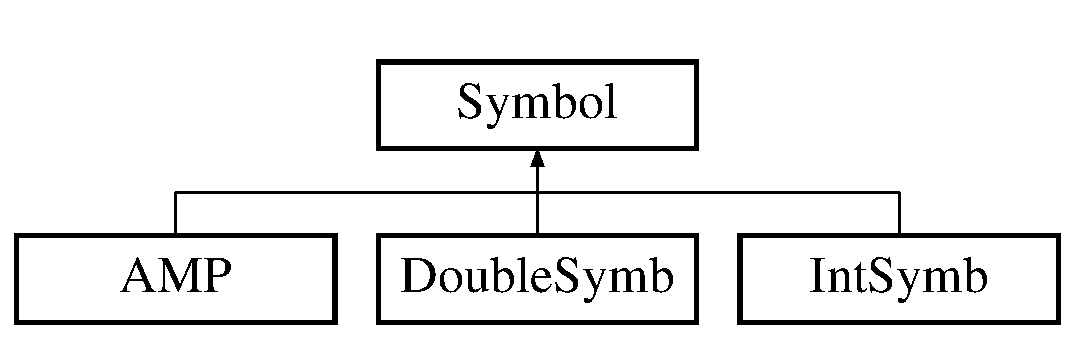
\includegraphics[height=2.000000cm]{class_symbol}
\end{center}
\end{figure}
\subsection*{Public Member Functions}
\begin{DoxyCompactItemize}
\item 
virtual std\+::stringstream \hyperlink{class_symbol_a327d7b38b13102918bab2a09b8b6a303}{print} ()=0
\item 
virtual \hyperlink{class_symbol}{Symbol} $\ast$ \hyperlink{class_symbol_ae8aeeef72df9b6c8f32197e97b909c72}{add} (\hyperlink{class_symbol}{Symbol} $\ast$operand)=0
\item 
virtual \hyperlink{class_symbol}{Symbol} $\ast$ \hyperlink{class_symbol_a53b98ce639c66d1b2e73992f20f56c54}{sub} (\hyperlink{class_symbol}{Symbol} $\ast$operand)=0
\item 
virtual \hyperlink{class_symbol}{Symbol} $\ast$ \hyperlink{class_symbol_a224ae5c870650b7704756d8279b9bc53}{mult} (\hyperlink{class_symbol}{Symbol} $\ast$operand)=0
\item 
virtual \hyperlink{class_symbol}{Symbol} $\ast$ \hyperlink{class_symbol_aa259102d6727f267c718b91c78e5eb46}{exp} (int exp)=0
\item 
virtual \hyperlink{class_symbol}{Symbol} $\ast$ \hyperlink{class_symbol_acfc77f36fef51f4d300896d0e5183986}{neg} ()=0
\item 
virtual \hyperlink{class_symbol}{Symbol} $\ast$ \hyperlink{class_symbol_a642df9ea636eb1b7fafa11fc539ea49a}{clone} ()=0
\item 
virtual \hyperlink{class_symbol_a0f129c4040fac10b29e9e9a3cddb2e69}{$\sim$\+Symbol} ()
\end{DoxyCompactItemize}
\subsection*{Protected Attributes}
\begin{DoxyCompactItemize}
\item 
bool \hyperlink{class_symbol_a4083674d0a03f08336b5767f3e83ddde}{is\+Var}
\end{DoxyCompactItemize}


\subsection{Detailed Description}


Definition at line 17 of file Symbol.\+h.



\subsection{Constructor \& Destructor Documentation}
\hypertarget{class_symbol_a0f129c4040fac10b29e9e9a3cddb2e69}{\index{Symbol@{Symbol}!````~Symbol@{$\sim$\+Symbol}}
\index{````~Symbol@{$\sim$\+Symbol}!Symbol@{Symbol}}
\subsubsection[{$\sim$\+Symbol}]{\setlength{\rightskip}{0pt plus 5cm}virtual Symbol\+::$\sim$\+Symbol (
\begin{DoxyParamCaption}
{}
\end{DoxyParamCaption}
)\hspace{0.3cm}{\ttfamily [inline]}, {\ttfamily [virtual]}}}\label{class_symbol_a0f129c4040fac10b29e9e9a3cddb2e69}


Definition at line 37 of file Symbol.\+h.



\subsection{Member Function Documentation}
\hypertarget{class_symbol_ae8aeeef72df9b6c8f32197e97b909c72}{\index{Symbol@{Symbol}!add@{add}}
\index{add@{add}!Symbol@{Symbol}}
\subsubsection[{add}]{\setlength{\rightskip}{0pt plus 5cm}virtual {\bf Symbol}$\ast$ Symbol\+::add (
\begin{DoxyParamCaption}
\item[{{\bf Symbol} $\ast$}]{operand}
\end{DoxyParamCaption}
)\hspace{0.3cm}{\ttfamily [pure virtual]}}}\label{class_symbol_ae8aeeef72df9b6c8f32197e97b909c72}


Implemented in \hyperlink{class_a_m_p_a13330b73b85994d48e091ba35d37f5da}{A\+M\+P}, \hyperlink{class_double_symb_a1d8cca63cce9963b43030891f1ff5e48}{Double\+Symb}, and \hyperlink{class_int_symb_a10885d3759e4a6765e8d564da4b53b2e}{Int\+Symb}.

\hypertarget{class_symbol_a642df9ea636eb1b7fafa11fc539ea49a}{\index{Symbol@{Symbol}!clone@{clone}}
\index{clone@{clone}!Symbol@{Symbol}}
\subsubsection[{clone}]{\setlength{\rightskip}{0pt plus 5cm}virtual {\bf Symbol}$\ast$ Symbol\+::clone (
\begin{DoxyParamCaption}
{}
\end{DoxyParamCaption}
)\hspace{0.3cm}{\ttfamily [pure virtual]}}}\label{class_symbol_a642df9ea636eb1b7fafa11fc539ea49a}


Implemented in \hyperlink{class_a_m_p_a7be3cf2bc62e7849d829412cd9e83875}{A\+M\+P}, \hyperlink{class_double_symb_a69077ea0fe3ed9eae80e3710e4be84e2}{Double\+Symb}, and \hyperlink{class_int_symb_a9a57c73450f2a93ca5ff93b0ad8f8aa9}{Int\+Symb}.

\hypertarget{class_symbol_aa259102d6727f267c718b91c78e5eb46}{\index{Symbol@{Symbol}!exp@{exp}}
\index{exp@{exp}!Symbol@{Symbol}}
\subsubsection[{exp}]{\setlength{\rightskip}{0pt plus 5cm}virtual {\bf Symbol}$\ast$ Symbol\+::exp (
\begin{DoxyParamCaption}
\item[{int}]{exp}
\end{DoxyParamCaption}
)\hspace{0.3cm}{\ttfamily [pure virtual]}}}\label{class_symbol_aa259102d6727f267c718b91c78e5eb46}


Implemented in \hyperlink{class_a_m_p_a0c3ed1aeaa0a0974f0ea3f7f92dbe080}{A\+M\+P}, \hyperlink{class_double_symb_a3b632822ad185fce623724148c914b8c}{Double\+Symb}, and \hyperlink{class_int_symb_a39254e07e5adc1b4179a39dd8aed49f7}{Int\+Symb}.

\hypertarget{class_symbol_a224ae5c870650b7704756d8279b9bc53}{\index{Symbol@{Symbol}!mult@{mult}}
\index{mult@{mult}!Symbol@{Symbol}}
\subsubsection[{mult}]{\setlength{\rightskip}{0pt plus 5cm}virtual {\bf Symbol}$\ast$ Symbol\+::mult (
\begin{DoxyParamCaption}
\item[{{\bf Symbol} $\ast$}]{operand}
\end{DoxyParamCaption}
)\hspace{0.3cm}{\ttfamily [pure virtual]}}}\label{class_symbol_a224ae5c870650b7704756d8279b9bc53}


Implemented in \hyperlink{class_a_m_p_ab9c9e14b427261284a980f936ce64095}{A\+M\+P}, \hyperlink{class_double_symb_a7b297714a165576a11ab7ba6b8990f0a}{Double\+Symb}, and \hyperlink{class_int_symb_ad0b2bd020dfd9c924cac7f722e8aac7e}{Int\+Symb}.

\hypertarget{class_symbol_acfc77f36fef51f4d300896d0e5183986}{\index{Symbol@{Symbol}!neg@{neg}}
\index{neg@{neg}!Symbol@{Symbol}}
\subsubsection[{neg}]{\setlength{\rightskip}{0pt plus 5cm}virtual {\bf Symbol}$\ast$ Symbol\+::neg (
\begin{DoxyParamCaption}
{}
\end{DoxyParamCaption}
)\hspace{0.3cm}{\ttfamily [pure virtual]}}}\label{class_symbol_acfc77f36fef51f4d300896d0e5183986}


Implemented in \hyperlink{class_a_m_p_aacc63b07222e5a3e1d3008ffcf8564c2}{A\+M\+P}, \hyperlink{class_double_symb_a36170febbfcd8709841050db05e6415b}{Double\+Symb}, and \hyperlink{class_int_symb_a24d2b18787ec241f268f3e8c259e6e64}{Int\+Symb}.

\hypertarget{class_symbol_a327d7b38b13102918bab2a09b8b6a303}{\index{Symbol@{Symbol}!print@{print}}
\index{print@{print}!Symbol@{Symbol}}
\subsubsection[{print}]{\setlength{\rightskip}{0pt plus 5cm}virtual std\+::stringstream Symbol\+::print (
\begin{DoxyParamCaption}
{}
\end{DoxyParamCaption}
)\hspace{0.3cm}{\ttfamily [pure virtual]}}}\label{class_symbol_a327d7b38b13102918bab2a09b8b6a303}


Implemented in \hyperlink{class_a_m_p_a0d97f7941390b745d4a8c5099f8530c1}{A\+M\+P}, \hyperlink{class_double_symb_a6bb7ecda5dfda94ecb658733eafc2f38}{Double\+Symb}, and \hyperlink{class_int_symb_a22115e6d6a513977d4cdad1013cdd15d}{Int\+Symb}.

\hypertarget{class_symbol_a53b98ce639c66d1b2e73992f20f56c54}{\index{Symbol@{Symbol}!sub@{sub}}
\index{sub@{sub}!Symbol@{Symbol}}
\subsubsection[{sub}]{\setlength{\rightskip}{0pt plus 5cm}virtual {\bf Symbol}$\ast$ Symbol\+::sub (
\begin{DoxyParamCaption}
\item[{{\bf Symbol} $\ast$}]{operand}
\end{DoxyParamCaption}
)\hspace{0.3cm}{\ttfamily [pure virtual]}}}\label{class_symbol_a53b98ce639c66d1b2e73992f20f56c54}


Implemented in \hyperlink{class_a_m_p_aa22f858fe19e8d00dea47ee9a6c26040}{A\+M\+P}, \hyperlink{class_double_symb_a0c08d8436a47c3d9e96d19aa80a2bab9}{Double\+Symb}, and \hyperlink{class_int_symb_ad4dd7298bf4a8ea002e86671a96f77d9}{Int\+Symb}.



\subsection{Member Data Documentation}
\hypertarget{class_symbol_a4083674d0a03f08336b5767f3e83ddde}{\index{Symbol@{Symbol}!is\+Var@{is\+Var}}
\index{is\+Var@{is\+Var}!Symbol@{Symbol}}
\subsubsection[{is\+Var}]{\setlength{\rightskip}{0pt plus 5cm}bool Symbol\+::is\+Var\hspace{0.3cm}{\ttfamily [protected]}}}\label{class_symbol_a4083674d0a03f08336b5767f3e83ddde}


Definition at line 20 of file Symbol.\+h.



The documentation for this class was generated from the following file\+:\begin{DoxyCompactItemize}
\item 
S\+L\+P/\hyperlink{_symbol_8h}{Symbol.\+h}\end{DoxyCompactItemize}

\hypertarget{class_vector}{\section{Vector$<$ T $>$ Class Template Reference}
\label{class_vector}\index{Vector$<$ T $>$@{Vector$<$ T $>$}}
}


{\ttfamily \#include $<$vec.\+h$>$}

\subsection*{Public Types}
\begin{DoxyCompactItemize}
\item 
typedef \hyperlink{vec_8h_a2dedc729e88b5f13d52bc9aeeda264dc}{Subscript} \hyperlink{class_vector_af11e5408e13f84b5de506db7681cf46e}{size\+\_\+type}
\item 
typedef T \hyperlink{class_vector_a79be47483938eb902a0a5af772985850}{value\+\_\+type}
\item 
typedef T \hyperlink{class_vector_a89d40fb2fabe6e0576ad9de72e829df1}{element\+\_\+type}
\item 
typedef T $\ast$ \hyperlink{class_vector_a79c196184d53dc1e6c4f7841392e528e}{pointer}
\item 
typedef T $\ast$ \hyperlink{class_vector_a30c203480dfd28a0f1fde5c08a68db94}{iterator}
\item 
typedef T \& \hyperlink{class_vector_aacab8f5d93fda39cbdf810e3440d1c29}{reference}
\item 
typedef const T $\ast$ \hyperlink{class_vector_acbec6290edaeacd3b3b72f39bf910365}{const\+\_\+iterator}
\item 
typedef const T \& \hyperlink{class_vector_a44d455da2c2c75f0ffda9856aa52308d}{const\+\_\+reference}
\end{DoxyCompactItemize}
\subsection*{Public Member Functions}
\begin{DoxyCompactItemize}
\item 
\hyperlink{vec_8h_a2dedc729e88b5f13d52bc9aeeda264dc}{Subscript} \hyperlink{class_vector_a1572f8f1f51c91ca1244ad4007554419}{lbound} () const 
\item 
\hyperlink{class_vector_a30c203480dfd28a0f1fde5c08a68db94}{iterator} \hyperlink{class_vector_a466e8c045ea10d62c28b689888e9fe5a}{begin} ()
\item 
\hyperlink{class_vector_a30c203480dfd28a0f1fde5c08a68db94}{iterator} \hyperlink{class_vector_ae288fa619188bff101d5300b8aaf9a90}{end} ()
\item 
const \hyperlink{class_vector_a30c203480dfd28a0f1fde5c08a68db94}{iterator} \hyperlink{class_vector_ae788da34b714381b90142b195d62fd42}{begin} () const 
\item 
const \hyperlink{class_vector_a30c203480dfd28a0f1fde5c08a68db94}{iterator} \hyperlink{class_vector_a89b541445053d883ad244ba5a7e49fbb}{end} () const 
\item 
\hyperlink{class_vector_afd524fac19e6d3d69db5198ffe2952b0}{$\sim$\+Vector} ()
\item 
\hyperlink{class_vector_a39d6069675db4ecfc1ab81d440da759a}{Vector} ()
\item 
\hyperlink{class_vector_a1687554d658dc6cf062f5a9c47b2bfdc}{Vector} (const \hyperlink{class_vector}{Vector}$<$ T $>$ \&A)
\item 
\hyperlink{class_vector_a82501ca0ed78bc60797e61429988ba5f}{Vector} (\hyperlink{vec_8h_a2dedc729e88b5f13d52bc9aeeda264dc}{Subscript} N, const T \&value=T(0))
\item 
\hyperlink{class_vector_aeb3281a2f62d066cecdd8d78f5758e9a}{Vector} (\hyperlink{vec_8h_a2dedc729e88b5f13d52bc9aeeda264dc}{Subscript} N, const T $\ast$v)
\item 
\hyperlink{class_vector_ac7cb3f96e3adb4bd02d075480849dd43}{Vector} (\hyperlink{vec_8h_a2dedc729e88b5f13d52bc9aeeda264dc}{Subscript} N, char $\ast$s)
\item 
\hyperlink{class_vector}{Vector}$<$ T $>$ \& \hyperlink{class_vector_a98e75f046dc4ed19e833c1fd79d7a15b}{newsize} (\hyperlink{vec_8h_a2dedc729e88b5f13d52bc9aeeda264dc}{Subscript} N)
\item 
\hyperlink{class_vector}{Vector}$<$ T $>$ \& \hyperlink{class_vector_a7b134c71c1f210b7df5c8025780e9740}{operator=} (const \hyperlink{class_vector}{Vector}$<$ T $>$ \&A)
\item 
\hyperlink{class_vector}{Vector}$<$ T $>$ \& \hyperlink{class_vector_a2e5185fbf998e9f599641db714d7efa5}{operator=} (const T \&scalar)
\item 
\hyperlink{vec_8h_a2dedc729e88b5f13d52bc9aeeda264dc}{Subscript} \hyperlink{class_vector_a709e7cbc009b3422d4571631a7dd921b}{dim} () const 
\item 
\hyperlink{vec_8h_a2dedc729e88b5f13d52bc9aeeda264dc}{Subscript} \hyperlink{class_vector_afde82844208cffe770402780c9d6538f}{size} () const 
\item 
\hyperlink{class_vector_aacab8f5d93fda39cbdf810e3440d1c29}{reference} \hyperlink{class_vector_a6da8486f6d5f590315568dd7fe521be0}{operator()} (\hyperlink{vec_8h_a2dedc729e88b5f13d52bc9aeeda264dc}{Subscript} i)
\item 
\hyperlink{class_vector_a44d455da2c2c75f0ffda9856aa52308d}{const\+\_\+reference} \hyperlink{class_vector_aa04fb25900a745548aa2354ed0f4fda4}{operator()} (\hyperlink{vec_8h_a2dedc729e88b5f13d52bc9aeeda264dc}{Subscript} i) const 
\item 
\hyperlink{class_vector_aacab8f5d93fda39cbdf810e3440d1c29}{reference} \hyperlink{class_vector_a9e29b5bf3394ef1dcff37e239c1ad5a5}{operator\mbox{[}$\,$\mbox{]}} (\hyperlink{vec_8h_a2dedc729e88b5f13d52bc9aeeda264dc}{Subscript} i)
\item 
\hyperlink{class_vector_a44d455da2c2c75f0ffda9856aa52308d}{const\+\_\+reference} \hyperlink{class_vector_a44f63672e86aedd66fa48deee29d191e}{operator\mbox{[}$\,$\mbox{]}} (\hyperlink{vec_8h_a2dedc729e88b5f13d52bc9aeeda264dc}{Subscript} i) const 
\item 
double \hyperlink{class_vector_a7662f254a0c62df3d02e92b575f7d5ac}{l2norm} ()
\item 
double \hyperlink{class_vector_a3c8c4aa22b451c5c416fb25a627fc0b8}{l2norm\+\_\+sqr} ()
\end{DoxyCompactItemize}
\subsection*{Protected Member Functions}
\begin{DoxyCompactItemize}
\item 
void \hyperlink{class_vector_a57325431d39d428c5c14b2ccb7849f50}{initialize} (\hyperlink{vec_8h_a2dedc729e88b5f13d52bc9aeeda264dc}{Subscript} N)
\item 
void \hyperlink{class_vector_a44a9d4be6b71e4e8db60f9249cd59a4b}{copy} (const T $\ast$v)
\item 
void \hyperlink{class_vector_aa2b58b0013fb00821d8ed3b666253557}{set} (const T \&val)
\item 
void \hyperlink{class_vector_a557dae0338b7c4f08a58cae39a7df869}{destroy} ()
\end{DoxyCompactItemize}
\subsection*{Protected Attributes}
\begin{DoxyCompactItemize}
\item 
T $\ast$ \hyperlink{class_vector_a35e75689eb9e46f564a5eaf515c73b72}{v\+\_\+}
\item 
T $\ast$ \hyperlink{class_vector_a5fe8f82950fdae7d3a8f2405e66bbbbc}{vm1\+\_\+}
\item 
\hyperlink{vec_8h_a2dedc729e88b5f13d52bc9aeeda264dc}{Subscript} \hyperlink{class_vector_a163c6b74af740a53f7cddc72c4d32978}{n\+\_\+}
\end{DoxyCompactItemize}
\subsection*{Friends}
\begin{DoxyCompactItemize}
\item 
bool \hyperlink{class_vector_a463b93549af3a1b5106e42b9e26cc7a1}{isnear} (const \hyperlink{class_vector}{Vector}$<$ T $>$ \&A, const \hyperlink{class_vector}{Vector}$<$ T $>$ \&B, const T tolerance)
\item 
bool \hyperlink{class_vector_ae8a7164cace28ff215b1d2b9d0e8a092}{operator==} (const \hyperlink{class_vector}{Vector}$<$ T $>$ \&A, const \hyperlink{class_vector}{Vector}$<$ T $>$ \&B)
\item 
bool \hyperlink{class_vector_ac833e0191dee06fa44ac6b49877336dc}{operator!=} (const \hyperlink{class_vector}{Vector}$<$ T $>$ \&A, const \hyperlink{class_vector}{Vector}$<$ T $>$ \&B)
\item 
istream \& \hyperlink{class_vector_a05030005479a3bd6c80f279f60e04568}{operator$>$$>$} (istream \&s, \hyperlink{class_vector}{Vector}$<$ T $>$ \&A)
\end{DoxyCompactItemize}


\subsection{Detailed Description}
\subsubsection*{template$<$class T$>$class Vector$<$ T $>$}



Definition at line 70 of file vec.\+h.



\subsection{Member Typedef Documentation}
\hypertarget{class_vector_acbec6290edaeacd3b3b72f39bf910365}{\index{Vector@{Vector}!const\+\_\+iterator@{const\+\_\+iterator}}
\index{const\+\_\+iterator@{const\+\_\+iterator}!Vector@{Vector}}
\subsubsection[{const\+\_\+iterator}]{\setlength{\rightskip}{0pt plus 5cm}template$<$class T$>$ typedef const T$\ast$ {\bf Vector}$<$ T $>$\+::{\bf const\+\_\+iterator}}}\label{class_vector_acbec6290edaeacd3b3b72f39bf910365}


Definition at line 82 of file vec.\+h.

\hypertarget{class_vector_a44d455da2c2c75f0ffda9856aa52308d}{\index{Vector@{Vector}!const\+\_\+reference@{const\+\_\+reference}}
\index{const\+\_\+reference@{const\+\_\+reference}!Vector@{Vector}}
\subsubsection[{const\+\_\+reference}]{\setlength{\rightskip}{0pt plus 5cm}template$<$class T$>$ typedef const T\& {\bf Vector}$<$ T $>$\+::{\bf const\+\_\+reference}}}\label{class_vector_a44d455da2c2c75f0ffda9856aa52308d}


Definition at line 83 of file vec.\+h.

\hypertarget{class_vector_a89d40fb2fabe6e0576ad9de72e829df1}{\index{Vector@{Vector}!element\+\_\+type@{element\+\_\+type}}
\index{element\+\_\+type@{element\+\_\+type}!Vector@{Vector}}
\subsubsection[{element\+\_\+type}]{\setlength{\rightskip}{0pt plus 5cm}template$<$class T$>$ typedef T {\bf Vector}$<$ T $>$\+::{\bf element\+\_\+type}}}\label{class_vector_a89d40fb2fabe6e0576ad9de72e829df1}


Definition at line 78 of file vec.\+h.

\hypertarget{class_vector_a30c203480dfd28a0f1fde5c08a68db94}{\index{Vector@{Vector}!iterator@{iterator}}
\index{iterator@{iterator}!Vector@{Vector}}
\subsubsection[{iterator}]{\setlength{\rightskip}{0pt plus 5cm}template$<$class T$>$ typedef T$\ast$ {\bf Vector}$<$ T $>$\+::{\bf iterator}}}\label{class_vector_a30c203480dfd28a0f1fde5c08a68db94}


Definition at line 80 of file vec.\+h.

\hypertarget{class_vector_a79c196184d53dc1e6c4f7841392e528e}{\index{Vector@{Vector}!pointer@{pointer}}
\index{pointer@{pointer}!Vector@{Vector}}
\subsubsection[{pointer}]{\setlength{\rightskip}{0pt plus 5cm}template$<$class T$>$ typedef T$\ast$ {\bf Vector}$<$ T $>$\+::{\bf pointer}}}\label{class_vector_a79c196184d53dc1e6c4f7841392e528e}


Definition at line 79 of file vec.\+h.

\hypertarget{class_vector_aacab8f5d93fda39cbdf810e3440d1c29}{\index{Vector@{Vector}!reference@{reference}}
\index{reference@{reference}!Vector@{Vector}}
\subsubsection[{reference}]{\setlength{\rightskip}{0pt plus 5cm}template$<$class T$>$ typedef T\& {\bf Vector}$<$ T $>$\+::{\bf reference}}}\label{class_vector_aacab8f5d93fda39cbdf810e3440d1c29}


Definition at line 81 of file vec.\+h.

\hypertarget{class_vector_af11e5408e13f84b5de506db7681cf46e}{\index{Vector@{Vector}!size\+\_\+type@{size\+\_\+type}}
\index{size\+\_\+type@{size\+\_\+type}!Vector@{Vector}}
\subsubsection[{size\+\_\+type}]{\setlength{\rightskip}{0pt plus 5cm}template$<$class T$>$ typedef {\bf Subscript} {\bf Vector}$<$ T $>$\+::{\bf size\+\_\+type}}}\label{class_vector_af11e5408e13f84b5de506db7681cf46e}


Definition at line 76 of file vec.\+h.

\hypertarget{class_vector_a79be47483938eb902a0a5af772985850}{\index{Vector@{Vector}!value\+\_\+type@{value\+\_\+type}}
\index{value\+\_\+type@{value\+\_\+type}!Vector@{Vector}}
\subsubsection[{value\+\_\+type}]{\setlength{\rightskip}{0pt plus 5cm}template$<$class T$>$ typedef T {\bf Vector}$<$ T $>$\+::{\bf value\+\_\+type}}}\label{class_vector_a79be47483938eb902a0a5af772985850}


Definition at line 77 of file vec.\+h.



\subsection{Constructor \& Destructor Documentation}
\hypertarget{class_vector_afd524fac19e6d3d69db5198ffe2952b0}{\index{Vector@{Vector}!````~Vector@{$\sim$\+Vector}}
\index{````~Vector@{$\sim$\+Vector}!Vector@{Vector}}
\subsubsection[{$\sim$\+Vector}]{\setlength{\rightskip}{0pt plus 5cm}template$<$class T$>$ {\bf Vector}$<$ T $>$\+::$\sim${\bf Vector} (
\begin{DoxyParamCaption}
{}
\end{DoxyParamCaption}
)\hspace{0.3cm}{\ttfamily [inline]}}}\label{class_vector_afd524fac19e6d3d69db5198ffe2952b0}


Definition at line 198 of file vec.\+h.

\hypertarget{class_vector_a39d6069675db4ecfc1ab81d440da759a}{\index{Vector@{Vector}!Vector@{Vector}}
\index{Vector@{Vector}!Vector@{Vector}}
\subsubsection[{Vector}]{\setlength{\rightskip}{0pt plus 5cm}template$<$class T$>$ {\bf Vector}$<$ T $>$\+::{\bf Vector} (
\begin{DoxyParamCaption}
{}
\end{DoxyParamCaption}
)\hspace{0.3cm}{\ttfamily [inline]}}}\label{class_vector_a39d6069675db4ecfc1ab81d440da759a}


Definition at line 205 of file vec.\+h.

\hypertarget{class_vector_a1687554d658dc6cf062f5a9c47b2bfdc}{\index{Vector@{Vector}!Vector@{Vector}}
\index{Vector@{Vector}!Vector@{Vector}}
\subsubsection[{Vector}]{\setlength{\rightskip}{0pt plus 5cm}template$<$class T$>$ {\bf Vector}$<$ T $>$\+::{\bf Vector} (
\begin{DoxyParamCaption}
\item[{const {\bf Vector}$<$ T $>$ \&}]{A}
\end{DoxyParamCaption}
)\hspace{0.3cm}{\ttfamily [inline]}}}\label{class_vector_a1687554d658dc6cf062f5a9c47b2bfdc}


Definition at line 207 of file vec.\+h.

\hypertarget{class_vector_a82501ca0ed78bc60797e61429988ba5f}{\index{Vector@{Vector}!Vector@{Vector}}
\index{Vector@{Vector}!Vector@{Vector}}
\subsubsection[{Vector}]{\setlength{\rightskip}{0pt plus 5cm}template$<$class T$>$ {\bf Vector}$<$ T $>$\+::{\bf Vector} (
\begin{DoxyParamCaption}
\item[{{\bf Subscript}}]{N, }
\item[{const T \&}]{value = {\ttfamily T(0)}}
\end{DoxyParamCaption}
)\hspace{0.3cm}{\ttfamily [inline]}}}\label{class_vector_a82501ca0ed78bc60797e61429988ba5f}


Definition at line 213 of file vec.\+h.

\hypertarget{class_vector_aeb3281a2f62d066cecdd8d78f5758e9a}{\index{Vector@{Vector}!Vector@{Vector}}
\index{Vector@{Vector}!Vector@{Vector}}
\subsubsection[{Vector}]{\setlength{\rightskip}{0pt plus 5cm}template$<$class T$>$ {\bf Vector}$<$ T $>$\+::{\bf Vector} (
\begin{DoxyParamCaption}
\item[{{\bf Subscript}}]{N, }
\item[{const T $\ast$}]{v}
\end{DoxyParamCaption}
)\hspace{0.3cm}{\ttfamily [inline]}}}\label{class_vector_aeb3281a2f62d066cecdd8d78f5758e9a}


Definition at line 219 of file vec.\+h.

\hypertarget{class_vector_ac7cb3f96e3adb4bd02d075480849dd43}{\index{Vector@{Vector}!Vector@{Vector}}
\index{Vector@{Vector}!Vector@{Vector}}
\subsubsection[{Vector}]{\setlength{\rightskip}{0pt plus 5cm}template$<$class T$>$ {\bf Vector}$<$ T $>$\+::{\bf Vector} (
\begin{DoxyParamCaption}
\item[{{\bf Subscript}}]{N, }
\item[{char $\ast$}]{s}
\end{DoxyParamCaption}
)\hspace{0.3cm}{\ttfamily [inline]}}}\label{class_vector_ac7cb3f96e3adb4bd02d075480849dd43}


Definition at line 225 of file vec.\+h.



\subsection{Member Function Documentation}
\hypertarget{class_vector_a466e8c045ea10d62c28b689888e9fe5a}{\index{Vector@{Vector}!begin@{begin}}
\index{begin@{begin}!Vector@{Vector}}
\subsubsection[{begin}]{\setlength{\rightskip}{0pt plus 5cm}template$<$class T$>$ {\bf iterator} {\bf Vector}$<$ T $>$\+::begin (
\begin{DoxyParamCaption}
{}
\end{DoxyParamCaption}
)\hspace{0.3cm}{\ttfamily [inline]}}}\label{class_vector_a466e8c045ea10d62c28b689888e9fe5a}


Definition at line 191 of file vec.\+h.

\hypertarget{class_vector_ae788da34b714381b90142b195d62fd42}{\index{Vector@{Vector}!begin@{begin}}
\index{begin@{begin}!Vector@{Vector}}
\subsubsection[{begin}]{\setlength{\rightskip}{0pt plus 5cm}template$<$class T$>$ const {\bf iterator} {\bf Vector}$<$ T $>$\+::begin (
\begin{DoxyParamCaption}
{}
\end{DoxyParamCaption}
) const\hspace{0.3cm}{\ttfamily [inline]}}}\label{class_vector_ae788da34b714381b90142b195d62fd42}


Definition at line 193 of file vec.\+h.

\hypertarget{class_vector_a44a9d4be6b71e4e8db60f9249cd59a4b}{\index{Vector@{Vector}!copy@{copy}}
\index{copy@{copy}!Vector@{Vector}}
\subsubsection[{copy}]{\setlength{\rightskip}{0pt plus 5cm}template$<$class T$>$ void {\bf Vector}$<$ T $>$\+::copy (
\begin{DoxyParamCaption}
\item[{const T $\ast$}]{v}
\end{DoxyParamCaption}
)\hspace{0.3cm}{\ttfamily [inline]}, {\ttfamily [protected]}}}\label{class_vector_a44a9d4be6b71e4e8db60f9249cd59a4b}


Definition at line 119 of file vec.\+h.

\hypertarget{class_vector_a557dae0338b7c4f08a58cae39a7df869}{\index{Vector@{Vector}!destroy@{destroy}}
\index{destroy@{destroy}!Vector@{Vector}}
\subsubsection[{destroy}]{\setlength{\rightskip}{0pt plus 5cm}template$<$class T$>$ void {\bf Vector}$<$ T $>$\+::destroy (
\begin{DoxyParamCaption}
{}
\end{DoxyParamCaption}
)\hspace{0.3cm}{\ttfamily [inline]}, {\ttfamily [protected]}}}\label{class_vector_a557dae0338b7c4f08a58cae39a7df869}


Definition at line 174 of file vec.\+h.

\hypertarget{class_vector_a709e7cbc009b3422d4571631a7dd921b}{\index{Vector@{Vector}!dim@{dim}}
\index{dim@{dim}!Vector@{Vector}}
\subsubsection[{dim}]{\setlength{\rightskip}{0pt plus 5cm}template$<$class T$>$ {\bf Subscript} {\bf Vector}$<$ T $>$\+::dim (
\begin{DoxyParamCaption}
{}
\end{DoxyParamCaption}
) const\hspace{0.3cm}{\ttfamily [inline]}}}\label{class_vector_a709e7cbc009b3422d4571631a7dd921b}


Definition at line 276 of file vec.\+h.

\hypertarget{class_vector_ae288fa619188bff101d5300b8aaf9a90}{\index{Vector@{Vector}!end@{end}}
\index{end@{end}!Vector@{Vector}}
\subsubsection[{end}]{\setlength{\rightskip}{0pt plus 5cm}template$<$class T$>$ {\bf iterator} {\bf Vector}$<$ T $>$\+::end (
\begin{DoxyParamCaption}
{}
\end{DoxyParamCaption}
)\hspace{0.3cm}{\ttfamily [inline]}}}\label{class_vector_ae288fa619188bff101d5300b8aaf9a90}


Definition at line 192 of file vec.\+h.

\hypertarget{class_vector_a89b541445053d883ad244ba5a7e49fbb}{\index{Vector@{Vector}!end@{end}}
\index{end@{end}!Vector@{Vector}}
\subsubsection[{end}]{\setlength{\rightskip}{0pt plus 5cm}template$<$class T$>$ const {\bf iterator} {\bf Vector}$<$ T $>$\+::end (
\begin{DoxyParamCaption}
{}
\end{DoxyParamCaption}
) const\hspace{0.3cm}{\ttfamily [inline]}}}\label{class_vector_a89b541445053d883ad244ba5a7e49fbb}


Definition at line 194 of file vec.\+h.

\hypertarget{class_vector_a57325431d39d428c5c14b2ccb7849f50}{\index{Vector@{Vector}!initialize@{initialize}}
\index{initialize@{initialize}!Vector@{Vector}}
\subsubsection[{initialize}]{\setlength{\rightskip}{0pt plus 5cm}template$<$class T$>$ void {\bf Vector}$<$ T $>$\+::initialize (
\begin{DoxyParamCaption}
\item[{{\bf Subscript}}]{N}
\end{DoxyParamCaption}
)\hspace{0.3cm}{\ttfamily [inline]}, {\ttfamily [protected]}}}\label{class_vector_a57325431d39d428c5c14b2ccb7849f50}


Definition at line 95 of file vec.\+h.

\hypertarget{class_vector_a7662f254a0c62df3d02e92b575f7d5ac}{\index{Vector@{Vector}!l2norm@{l2norm}}
\index{l2norm@{l2norm}!Vector@{Vector}}
\subsubsection[{l2norm}]{\setlength{\rightskip}{0pt plus 5cm}template$<$class T$>$ double {\bf Vector}$<$ T $>$\+::l2norm (
\begin{DoxyParamCaption}
{}
\end{DoxyParamCaption}
)\hspace{0.3cm}{\ttfamily [inline]}}}\label{class_vector_a7662f254a0c62df3d02e92b575f7d5ac}


Definition at line 362 of file vec.\+h.

\hypertarget{class_vector_a3c8c4aa22b451c5c416fb25a627fc0b8}{\index{Vector@{Vector}!l2norm\+\_\+sqr@{l2norm\+\_\+sqr}}
\index{l2norm\+\_\+sqr@{l2norm\+\_\+sqr}!Vector@{Vector}}
\subsubsection[{l2norm\+\_\+sqr}]{\setlength{\rightskip}{0pt plus 5cm}template$<$class T$>$ double {\bf Vector}$<$ T $>$\+::l2norm\+\_\+sqr (
\begin{DoxyParamCaption}
{}
\end{DoxyParamCaption}
)\hspace{0.3cm}{\ttfamily [inline]}}}\label{class_vector_a3c8c4aa22b451c5c416fb25a627fc0b8}


Definition at line 403 of file vec.\+h.

\hypertarget{class_vector_a1572f8f1f51c91ca1244ad4007554419}{\index{Vector@{Vector}!lbound@{lbound}}
\index{lbound@{lbound}!Vector@{Vector}}
\subsubsection[{lbound}]{\setlength{\rightskip}{0pt plus 5cm}template$<$class T$>$ {\bf Subscript} {\bf Vector}$<$ T $>$\+::lbound (
\begin{DoxyParamCaption}
{}
\end{DoxyParamCaption}
) const\hspace{0.3cm}{\ttfamily [inline]}}}\label{class_vector_a1572f8f1f51c91ca1244ad4007554419}


Definition at line 85 of file vec.\+h.

\hypertarget{class_vector_a98e75f046dc4ed19e833c1fd79d7a15b}{\index{Vector@{Vector}!newsize@{newsize}}
\index{newsize@{newsize}!Vector@{Vector}}
\subsubsection[{newsize}]{\setlength{\rightskip}{0pt plus 5cm}template$<$class T$>$ {\bf Vector}$<$T$>$\& {\bf Vector}$<$ T $>$\+::newsize (
\begin{DoxyParamCaption}
\item[{{\bf Subscript}}]{N}
\end{DoxyParamCaption}
)\hspace{0.3cm}{\ttfamily [inline]}}}\label{class_vector_a98e75f046dc4ed19e833c1fd79d7a15b}


Definition at line 239 of file vec.\+h.

\hypertarget{class_vector_a6da8486f6d5f590315568dd7fe521be0}{\index{Vector@{Vector}!operator()@{operator()}}
\index{operator()@{operator()}!Vector@{Vector}}
\subsubsection[{operator()}]{\setlength{\rightskip}{0pt plus 5cm}template$<$class T$>$ {\bf reference} {\bf Vector}$<$ T $>$\+::operator() (
\begin{DoxyParamCaption}
\item[{{\bf Subscript}}]{i}
\end{DoxyParamCaption}
)\hspace{0.3cm}{\ttfamily [inline]}}}\label{class_vector_a6da8486f6d5f590315568dd7fe521be0}


Definition at line 315 of file vec.\+h.

\hypertarget{class_vector_aa04fb25900a745548aa2354ed0f4fda4}{\index{Vector@{Vector}!operator()@{operator()}}
\index{operator()@{operator()}!Vector@{Vector}}
\subsubsection[{operator()}]{\setlength{\rightskip}{0pt plus 5cm}template$<$class T$>$ {\bf const\+\_\+reference} {\bf Vector}$<$ T $>$\+::operator() (
\begin{DoxyParamCaption}
\item[{{\bf Subscript}}]{i}
\end{DoxyParamCaption}
) const\hspace{0.3cm}{\ttfamily [inline]}}}\label{class_vector_aa04fb25900a745548aa2354ed0f4fda4}


Definition at line 324 of file vec.\+h.

\hypertarget{class_vector_a7b134c71c1f210b7df5c8025780e9740}{\index{Vector@{Vector}!operator=@{operator=}}
\index{operator=@{operator=}!Vector@{Vector}}
\subsubsection[{operator=}]{\setlength{\rightskip}{0pt plus 5cm}template$<$class T$>$ {\bf Vector}$<$T$>$\& {\bf Vector}$<$ T $>$\+::operator= (
\begin{DoxyParamCaption}
\item[{const {\bf Vector}$<$ T $>$ \&}]{A}
\end{DoxyParamCaption}
)\hspace{0.3cm}{\ttfamily [inline]}}}\label{class_vector_a7b134c71c1f210b7df5c8025780e9740}


Definition at line 252 of file vec.\+h.

\hypertarget{class_vector_a2e5185fbf998e9f599641db714d7efa5}{\index{Vector@{Vector}!operator=@{operator=}}
\index{operator=@{operator=}!Vector@{Vector}}
\subsubsection[{operator=}]{\setlength{\rightskip}{0pt plus 5cm}template$<$class T$>$ {\bf Vector}$<$T$>$\& {\bf Vector}$<$ T $>$\+::operator= (
\begin{DoxyParamCaption}
\item[{const T \&}]{scalar}
\end{DoxyParamCaption}
)\hspace{0.3cm}{\ttfamily [inline]}}}\label{class_vector_a2e5185fbf998e9f599641db714d7efa5}


Definition at line 270 of file vec.\+h.

\hypertarget{class_vector_a9e29b5bf3394ef1dcff37e239c1ad5a5}{\index{Vector@{Vector}!operator\mbox{[}$\,$\mbox{]}@{operator[]}}
\index{operator\mbox{[}$\,$\mbox{]}@{operator[]}!Vector@{Vector}}
\subsubsection[{operator[]}]{\setlength{\rightskip}{0pt plus 5cm}template$<$class T$>$ {\bf reference} {\bf Vector}$<$ T $>$\+::operator\mbox{[}$\,$\mbox{]} (
\begin{DoxyParamCaption}
\item[{{\bf Subscript}}]{i}
\end{DoxyParamCaption}
)\hspace{0.3cm}{\ttfamily [inline]}}}\label{class_vector_a9e29b5bf3394ef1dcff37e239c1ad5a5}


Definition at line 333 of file vec.\+h.

\hypertarget{class_vector_a44f63672e86aedd66fa48deee29d191e}{\index{Vector@{Vector}!operator\mbox{[}$\,$\mbox{]}@{operator[]}}
\index{operator\mbox{[}$\,$\mbox{]}@{operator[]}!Vector@{Vector}}
\subsubsection[{operator[]}]{\setlength{\rightskip}{0pt plus 5cm}template$<$class T$>$ {\bf const\+\_\+reference} {\bf Vector}$<$ T $>$\+::operator\mbox{[}$\,$\mbox{]} (
\begin{DoxyParamCaption}
\item[{{\bf Subscript}}]{i}
\end{DoxyParamCaption}
) const\hspace{0.3cm}{\ttfamily [inline]}}}\label{class_vector_a44f63672e86aedd66fa48deee29d191e}


Definition at line 342 of file vec.\+h.

\hypertarget{class_vector_aa2b58b0013fb00821d8ed3b666253557}{\index{Vector@{Vector}!set@{set}}
\index{set@{set}!Vector@{Vector}}
\subsubsection[{set}]{\setlength{\rightskip}{0pt plus 5cm}template$<$class T$>$ void {\bf Vector}$<$ T $>$\+::set (
\begin{DoxyParamCaption}
\item[{const T \&}]{val}
\end{DoxyParamCaption}
)\hspace{0.3cm}{\ttfamily [inline]}, {\ttfamily [protected]}}}\label{class_vector_aa2b58b0013fb00821d8ed3b666253557}


Definition at line 145 of file vec.\+h.

\hypertarget{class_vector_afde82844208cffe770402780c9d6538f}{\index{Vector@{Vector}!size@{size}}
\index{size@{size}!Vector@{Vector}}
\subsubsection[{size}]{\setlength{\rightskip}{0pt plus 5cm}template$<$class T$>$ {\bf Subscript} {\bf Vector}$<$ T $>$\+::size (
\begin{DoxyParamCaption}
{}
\end{DoxyParamCaption}
) const\hspace{0.3cm}{\ttfamily [inline]}}}\label{class_vector_afde82844208cffe770402780c9d6538f}


Definition at line 281 of file vec.\+h.



\subsection{Friends And Related Function Documentation}
\hypertarget{class_vector_a463b93549af3a1b5106e42b9e26cc7a1}{\index{Vector@{Vector}!isnear@{isnear}}
\index{isnear@{isnear}!Vector@{Vector}}
\subsubsection[{isnear}]{\setlength{\rightskip}{0pt plus 5cm}template$<$class T$>$ bool isnear (
\begin{DoxyParamCaption}
\item[{const {\bf Vector}$<$ T $>$ \&}]{A, }
\item[{const {\bf Vector}$<$ T $>$ \&}]{B, }
\item[{const T}]{tolerance}
\end{DoxyParamCaption}
)\hspace{0.3cm}{\ttfamily [friend]}}}\label{class_vector_a463b93549af3a1b5106e42b9e26cc7a1}


Definition at line 288 of file vec.\+h.

\hypertarget{class_vector_ac833e0191dee06fa44ac6b49877336dc}{\index{Vector@{Vector}!operator"!=@{operator"!=}}
\index{operator"!=@{operator"!=}!Vector@{Vector}}
\subsubsection[{operator"!=}]{\setlength{\rightskip}{0pt plus 5cm}template$<$class T$>$ bool operator!= (
\begin{DoxyParamCaption}
\item[{const {\bf Vector}$<$ T $>$ \&}]{A, }
\item[{const {\bf Vector}$<$ T $>$ \&}]{B}
\end{DoxyParamCaption}
)\hspace{0.3cm}{\ttfamily [friend]}}}\label{class_vector_ac833e0191dee06fa44ac6b49877336dc}


Definition at line 308 of file vec.\+h.

\hypertarget{class_vector_ae8a7164cace28ff215b1d2b9d0e8a092}{\index{Vector@{Vector}!operator==@{operator==}}
\index{operator==@{operator==}!Vector@{Vector}}
\subsubsection[{operator==}]{\setlength{\rightskip}{0pt plus 5cm}template$<$class T$>$ bool operator== (
\begin{DoxyParamCaption}
\item[{const {\bf Vector}$<$ T $>$ \&}]{A, }
\item[{const {\bf Vector}$<$ T $>$ \&}]{B}
\end{DoxyParamCaption}
)\hspace{0.3cm}{\ttfamily [friend]}}}\label{class_vector_ae8a7164cace28ff215b1d2b9d0e8a092}


Definition at line 298 of file vec.\+h.

\hypertarget{class_vector_a05030005479a3bd6c80f279f60e04568}{\index{Vector@{Vector}!operator$>$$>$@{operator$>$$>$}}
\index{operator$>$$>$@{operator$>$$>$}!Vector@{Vector}}
\subsubsection[{operator$>$$>$}]{\setlength{\rightskip}{0pt plus 5cm}template$<$class T$>$ istream\& operator$>$$>$ (
\begin{DoxyParamCaption}
\item[{istream \&}]{s, }
\item[{{\bf Vector}$<$ T $>$ \&}]{A}
\end{DoxyParamCaption}
)\hspace{0.3cm}{\ttfamily [friend]}}}\label{class_vector_a05030005479a3bd6c80f279f60e04568}


Definition at line 463 of file vec.\+h.



\subsection{Member Data Documentation}
\hypertarget{class_vector_a163c6b74af740a53f7cddc72c4d32978}{\index{Vector@{Vector}!n\+\_\+@{n\+\_\+}}
\index{n\+\_\+@{n\+\_\+}!Vector@{Vector}}
\subsubsection[{n\+\_\+}]{\setlength{\rightskip}{0pt plus 5cm}template$<$class T$>$ {\bf Subscript} {\bf Vector}$<$ T $>$\+::n\+\_\+\hspace{0.3cm}{\ttfamily [protected]}}}\label{class_vector_a163c6b74af740a53f7cddc72c4d32978}


Definition at line 90 of file vec.\+h.

\hypertarget{class_vector_a35e75689eb9e46f564a5eaf515c73b72}{\index{Vector@{Vector}!v\+\_\+@{v\+\_\+}}
\index{v\+\_\+@{v\+\_\+}!Vector@{Vector}}
\subsubsection[{v\+\_\+}]{\setlength{\rightskip}{0pt plus 5cm}template$<$class T$>$ T$\ast$ {\bf Vector}$<$ T $>$\+::v\+\_\+\hspace{0.3cm}{\ttfamily [protected]}}}\label{class_vector_a35e75689eb9e46f564a5eaf515c73b72}


Definition at line 88 of file vec.\+h.

\hypertarget{class_vector_a5fe8f82950fdae7d3a8f2405e66bbbbc}{\index{Vector@{Vector}!vm1\+\_\+@{vm1\+\_\+}}
\index{vm1\+\_\+@{vm1\+\_\+}!Vector@{Vector}}
\subsubsection[{vm1\+\_\+}]{\setlength{\rightskip}{0pt plus 5cm}template$<$class T$>$ T$\ast$ {\bf Vector}$<$ T $>$\+::vm1\+\_\+\hspace{0.3cm}{\ttfamily [protected]}}}\label{class_vector_a5fe8f82950fdae7d3a8f2405e66bbbbc}


Definition at line 89 of file vec.\+h.



The documentation for this class was generated from the following file\+:\begin{DoxyCompactItemize}
\item 
\hyperlink{vec_8h}{vec.\+h}\end{DoxyCompactItemize}

\hypertarget{classvector}{\section{vector$<$ \+\_\+\+Ty, \+\_\+\+Ax $>$ Class Template Reference}
\label{classvector}\index{vector$<$ \+\_\+\+Ty, \+\_\+\+Ax $>$@{vector$<$ \+\_\+\+Ty, \+\_\+\+Ax $>$}}
}


{\ttfamily \#include $<$vector.\+h$>$}

Inheritance diagram for vector$<$ \+\_\+\+Ty, \+\_\+\+Ax $>$\+:\begin{figure}[H]
\begin{center}
\leavevmode
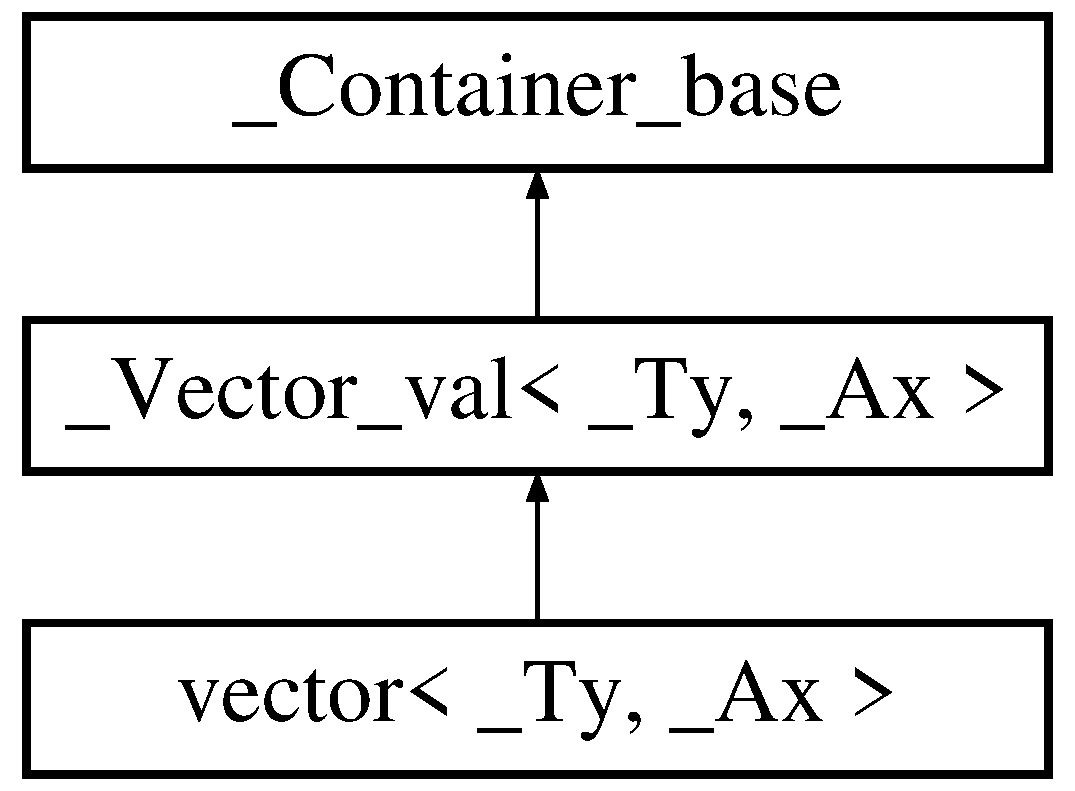
\includegraphics[height=3.000000cm]{classvector}
\end{center}
\end{figure}
\subsection*{Public Types}
\begin{DoxyCompactItemize}
\item 
typedef \hyperlink{classvector}{vector}$<$ \+\_\+\+Ty, \+\_\+\+Ax $>$ \hyperlink{classvector_ae499c665535254a7364e3a219b780112}{\+\_\+\+Myt}
\item 
typedef \hyperlink{class___vector__val}{\+\_\+\+Vector\+\_\+val}$<$ \+\_\+\+Ty, \+\_\+\+Ax $>$ \hyperlink{classvector_a1d0fa35df9c0b874ea870eae971fe5e0}{\+\_\+\+Mybase}
\item 
typedef \hyperlink{class___vector__val_ad273d1146bf265f65e75133aa2f9986a}{\+\_\+\+Mybase\+::\+\_\+\+Alty} \hyperlink{classvector_af95a9863612fdd67572c39c825c5aee6}{\+\_\+\+Alloc}
\item 
typedef \hyperlink{classvector_af95a9863612fdd67572c39c825c5aee6}{\+\_\+\+Alloc} \hyperlink{classvector_ae35ea7650735172fd02fdd94aa530a25}{allocator\+\_\+type}
\item 
typedef \+\_\+\+Alloc\+::size\+\_\+type \hyperlink{classvector_ac975e84f5d6c2fe2267bb354a85818af}{size\+\_\+type}
\item 
typedef \+\_\+\+Alloc\+::difference\+\_\+type \hyperlink{classvector_a5972097c9d52210f29e2d753a75b0a7a}{difference\+\_\+type}
\item 
typedef \+\_\+\+Alloc\+::pointer \hyperlink{classvector_a7f69707c8f1cc638260b523d48793523}{pointer}
\item 
typedef \+\_\+\+Alloc\+::const\+\_\+pointer \hyperlink{classvector_a52b51d85dd355481f31b8d1643d5b969}{const\+\_\+pointer}
\item 
typedef \+\_\+\+Alloc\+::reference \hyperlink{classvector_a68d6b0f887c9e4d0f422a1e3900b9794}{reference}
\item 
typedef \+\_\+\+Alloc\+::const\+\_\+reference \hyperlink{classvector_a22ae7381c38ba94955ba45177b24a51f}{const\+\_\+reference}
\item 
typedef \+\_\+\+Alloc\+::value\+\_\+type \hyperlink{classvector_acb600d25126cc0f3871b5a73f840acad}{value\+\_\+type}
\item 
typedef \hyperlink{class___vector__iterator}{\+\_\+\+Vector\+\_\+iterator}$<$ \hyperlink{classvector_a1d0fa35df9c0b874ea870eae971fe5e0}{\+\_\+\+Mybase} $>$ \hyperlink{classvector_a5a7a542bca0f55f43e161bd5a09c483d}{iterator}
\item 
typedef \hyperlink{class___vector__const__iterator}{\+\_\+\+Vector\+\_\+const\+\_\+iterator}\\*
$<$ \hyperlink{classvector_a1d0fa35df9c0b874ea870eae971fe5e0}{\+\_\+\+Mybase} $>$ \hyperlink{classvector_abed2910558c61a5a17113b2d250994da}{const\+\_\+iterator}
\item 
typedef \+\_\+\+S\+T\+D \hyperlink{classvector_a40def3e50f68e742f5b0cc571eaf51eb}{reverse\+\_\+iterator}\\*
$<$ \hyperlink{classvector_a5a7a542bca0f55f43e161bd5a09c483d}{iterator} $>$ \hyperlink{classvector_a40def3e50f68e742f5b0cc571eaf51eb}{reverse\+\_\+iterator}
\item 
typedef \+\_\+\+S\+T\+D \hyperlink{classvector_a40def3e50f68e742f5b0cc571eaf51eb}{reverse\+\_\+iterator}\\*
$<$ \hyperlink{classvector_abed2910558c61a5a17113b2d250994da}{const\+\_\+iterator} $>$ \hyperlink{classvector_aefbb12258ea747e127ef628e91e3c061}{const\+\_\+reverse\+\_\+iterator}
\end{DoxyCompactItemize}
\subsection*{Public Member Functions}
\begin{DoxyCompactItemize}
\item 
\hyperlink{classvector_a228c9f7f14ec03dc6c77b58ad336aef3}{vector} ()
\item 
\hyperlink{classvector_ab21a4ccb639ea9fd983deaf97ae08034}{vector} (const \hyperlink{classvector_af95a9863612fdd67572c39c825c5aee6}{\+\_\+\+Alloc} \&\+\_\+\+Al)
\item 
\hyperlink{classvector_a51699cf57fc396ee5e6d220cc443e1b9}{vector} (\hyperlink{classvector_ac975e84f5d6c2fe2267bb354a85818af}{size\+\_\+type} \+\_\+\+Count)
\item 
\hyperlink{classvector_a216cecdf1dce89b22e429f462f782c05}{vector} (\hyperlink{classvector_ac975e84f5d6c2fe2267bb354a85818af}{size\+\_\+type} \+\_\+\+Count, const \+\_\+\+Ty \&\+\_\+\+Val)
\item 
\hyperlink{classvector_aa42d2e860dd28f204fb63ff24c8d046d}{vector} (\hyperlink{classvector_ac975e84f5d6c2fe2267bb354a85818af}{size\+\_\+type} \+\_\+\+Count, const \+\_\+\+Ty \&\+\_\+\+Val, const \hyperlink{classvector_af95a9863612fdd67572c39c825c5aee6}{\+\_\+\+Alloc} \&\+\_\+\+Al)
\item 
\hyperlink{classvector_ad33fdaff980e232bc58ae3ffcc39b44a}{vector} (const \hyperlink{classvector_ae499c665535254a7364e3a219b780112}{\+\_\+\+Myt} \&\+\_\+\+Right)
\item 
{\footnotesize template$<$class \+\_\+\+Iter $>$ }\\\hyperlink{classvector_a91c17323d484d96fd650414a1b4355e5}{vector} (\+\_\+\+Iter \+\_\+\+First, \+\_\+\+Iter \+\_\+\+Last)
\item 
{\footnotesize template$<$class \+\_\+\+Iter $>$ }\\\hyperlink{classvector_a49286302a69b1ea41854e75183810cba}{vector} (\+\_\+\+Iter \+\_\+\+First, \+\_\+\+Iter \+\_\+\+Last, const \hyperlink{classvector_af95a9863612fdd67572c39c825c5aee6}{\+\_\+\+Alloc} \&\+\_\+\+Al)
\item 
{\footnotesize template$<$class \+\_\+\+Iter $>$ }\\void \hyperlink{classvector_af458407343307d48e496bad8e3aaecbf}{\+\_\+\+Construct} (\+\_\+\+Iter \+\_\+\+Count, \+\_\+\+Iter \+\_\+\+Val, \+\_\+\+Int\+\_\+iterator\+\_\+tag)
\item 
{\footnotesize template$<$class \+\_\+\+Iter $>$ }\\void \hyperlink{classvector_a8d6b5f89ce28d9e71f67500a96cefa45}{\+\_\+\+Construct} (\+\_\+\+Iter \+\_\+\+First, \+\_\+\+Iter \+\_\+\+Last, input\+\_\+iterator\+\_\+tag)
\item 
void \hyperlink{classvector_a37d757eaf6d72cf8b3d0e2195cacf188}{\+\_\+\+Construct\+\_\+n} (\hyperlink{classvector_ac975e84f5d6c2fe2267bb354a85818af}{size\+\_\+type} \+\_\+\+Count, const \+\_\+\+Ty $\ast$\+\_\+\+Pval)
\item 
\hyperlink{classvector_ad6d57100eef2daafdcc4628af06a656d}{vector} (\hyperlink{classvector_ae499c665535254a7364e3a219b780112}{\+\_\+\+Myt} \&\&\+\_\+\+Right)
\item 
\hyperlink{classvector_ae499c665535254a7364e3a219b780112}{\+\_\+\+Myt} \& \hyperlink{classvector_a209c9b772cdd5ed01ffc9d351a953826}{operator=} (\hyperlink{classvector_ae499c665535254a7364e3a219b780112}{\+\_\+\+Myt} \&\&\+\_\+\+Right)
\item 
void \hyperlink{classvector_a5b3c2d0a2573a1ed31a1ac9b7413f0f3}{\+\_\+\+Assign\+\_\+rv} (\hyperlink{classvector_ae499c665535254a7364e3a219b780112}{\+\_\+\+Myt} \&\&\+\_\+\+Right)
\item 
void \hyperlink{classvector_acf11e850cea519337e771d3d9d3779eb}{push\+\_\+back} (\+\_\+\+Ty \&\&\+\_\+\+Val)
\item 
void \hyperlink{classvector_a9a698dee99d62dd092caa7f17572866a}{emplace\+\_\+back} (\+\_\+\+Ty \&\&\+\_\+\+Val)
\item 
{\footnotesize template$<$class \+\_\+\+Valty $>$ }\\void \hyperlink{classvector_abd73be05a346e182658bbc1b1ae52dec}{emplace\+\_\+back} (\+\_\+\+Valty \&\&\+\_\+\+Val)
\item 
{\footnotesize template$<$class \+\_\+\+Valty $>$ }\\\hyperlink{classvector_a5a7a542bca0f55f43e161bd5a09c483d}{iterator} \hyperlink{classvector_ac52a3ac9c41a88dea7ab11fd73539893}{insert} (\hyperlink{classvector_abed2910558c61a5a17113b2d250994da}{const\+\_\+iterator} \+\_\+\+Where, \+\_\+\+Valty \&\&\+\_\+\+Val)
\item 
{\footnotesize template$<$class \+\_\+\+Valty $>$ }\\\hyperlink{classvector_a5a7a542bca0f55f43e161bd5a09c483d}{iterator} \hyperlink{classvector_abd24d07d48fcb842a6d07d2e7f0578dc}{emplace} (\hyperlink{classvector_abed2910558c61a5a17113b2d250994da}{const\+\_\+iterator} \+\_\+\+Where, \+\_\+\+Valty \&\&\+\_\+\+Val)
\item 
void \hyperlink{classvector_a949b2559806ecaae9cd5e3fcbec75d95}{swap} (\hyperlink{classvector_ae499c665535254a7364e3a219b780112}{\+\_\+\+Myt} \&\&\+\_\+\+Right)
\item 
\hyperlink{classvector_a98318c18baf337cfd287144557edb20c}{$\sim$vector} ()
\item 
\hyperlink{classvector_ae499c665535254a7364e3a219b780112}{\+\_\+\+Myt} \& \hyperlink{classvector_a5d402c01180b25eeb170866e2717b725}{operator=} (const \hyperlink{classvector_ae499c665535254a7364e3a219b780112}{\+\_\+\+Myt} \&\+\_\+\+Right)
\item 
void \hyperlink{classvector_a7428e66207efbf468e49651985a08c31}{reserve} (\hyperlink{classvector_ac975e84f5d6c2fe2267bb354a85818af}{size\+\_\+type} \+\_\+\+Count)
\item 
\hyperlink{classvector_ac975e84f5d6c2fe2267bb354a85818af}{size\+\_\+type} \hyperlink{classvector_a21c65889147afae2659222cd573aeb6e}{capacity} () const 
\item 
\hyperlink{classvector_a5a7a542bca0f55f43e161bd5a09c483d}{iterator} \hyperlink{classvector_a6efe00923de326e1661c331968658cf6}{begin} ()
\item 
\hyperlink{classvector_abed2910558c61a5a17113b2d250994da}{const\+\_\+iterator} \hyperlink{classvector_a7852e2f2214cf8b6c35cc37fd403ad3c}{begin} () const 
\item 
\hyperlink{classvector_a5a7a542bca0f55f43e161bd5a09c483d}{iterator} \hyperlink{classvector_aba1634590994c68b16af21735a4f541a}{end} ()
\item 
\hyperlink{classvector_abed2910558c61a5a17113b2d250994da}{const\+\_\+iterator} \hyperlink{classvector_a5ddbe02dc2954e254f93eb33dc03c9c8}{end} () const 
\item 
\hyperlink{classvector_a5a7a542bca0f55f43e161bd5a09c483d}{iterator} \hyperlink{classvector_a3957e92146489f5d04e5075dec2858cb}{\+\_\+\+Make\+\_\+iter} (\hyperlink{classvector_abed2910558c61a5a17113b2d250994da}{const\+\_\+iterator} \+\_\+\+Where) const 
\item 
\hyperlink{classvector_a40def3e50f68e742f5b0cc571eaf51eb}{reverse\+\_\+iterator} \hyperlink{classvector_a78f8334976fd4cb3954b1fe0833f7d90}{rbegin} ()
\item 
\hyperlink{classvector_aefbb12258ea747e127ef628e91e3c061}{const\+\_\+reverse\+\_\+iterator} \hyperlink{classvector_ae885bc2d89e2e938acf68437b618249b}{rbegin} () const 
\item 
\hyperlink{classvector_a40def3e50f68e742f5b0cc571eaf51eb}{reverse\+\_\+iterator} \hyperlink{classvector_ace499734c8f59823a305d8ee8355faf4}{rend} ()
\item 
\hyperlink{classvector_aefbb12258ea747e127ef628e91e3c061}{const\+\_\+reverse\+\_\+iterator} \hyperlink{classvector_a5d33de9ba4b238f1baeb6ae178d6725a}{rend} () const 
\item 
void \hyperlink{classvector_aa98dbcc4560cd1171d5d6d23567e8d53}{resize} (\hyperlink{classvector_ac975e84f5d6c2fe2267bb354a85818af}{size\+\_\+type} \+\_\+\+Newsize)
\item 
void \hyperlink{classvector_a7bc8f8fd18dfea8648036ba31f616386}{resize} (\hyperlink{classvector_ac975e84f5d6c2fe2267bb354a85818af}{size\+\_\+type} \+\_\+\+Newsize, \+\_\+\+Ty \+\_\+\+Val)
\item 
\hyperlink{classvector_ac975e84f5d6c2fe2267bb354a85818af}{size\+\_\+type} \hyperlink{classvector_a1f753ec0d05eadcb7fc18617ea54a82b}{size} () const 
\item 
\hyperlink{classvector_ac975e84f5d6c2fe2267bb354a85818af}{size\+\_\+type} \hyperlink{classvector_a0002515b016b6ea9ba25902c44ec7b1a}{max\+\_\+size} () const 
\item 
bool \hyperlink{classvector_a8aa620f8d84b5a9b2279d0956039da25}{empty} () const 
\item 
\hyperlink{classvector_af95a9863612fdd67572c39c825c5aee6}{\+\_\+\+Alloc} \hyperlink{classvector_a0ee6657761474e25e5d0c33926b1f7f7}{get\+\_\+allocator} () const 
\item 
\hyperlink{classvector_a22ae7381c38ba94955ba45177b24a51f}{const\+\_\+reference} \hyperlink{classvector_abb4ef2cdcb5fe5fd4f67abbf4135765c}{at} (\hyperlink{classvector_ac975e84f5d6c2fe2267bb354a85818af}{size\+\_\+type} \+\_\+\+Pos) const 
\item 
\hyperlink{classvector_a68d6b0f887c9e4d0f422a1e3900b9794}{reference} \hyperlink{classvector_af83e91556a8a2ea79e558c8d62bd442b}{at} (\hyperlink{classvector_ac975e84f5d6c2fe2267bb354a85818af}{size\+\_\+type} \+\_\+\+Pos)
\item 
\hyperlink{classvector_a22ae7381c38ba94955ba45177b24a51f}{const\+\_\+reference} \hyperlink{classvector_aa364f7385b52acc5e9931fb1e9af09d7}{operator\mbox{[}$\,$\mbox{]}} (\hyperlink{classvector_ac975e84f5d6c2fe2267bb354a85818af}{size\+\_\+type} \+\_\+\+Pos) const 
\item 
\hyperlink{classvector_a68d6b0f887c9e4d0f422a1e3900b9794}{reference} \hyperlink{classvector_a193ab55a199d22c1f47c190343a535fa}{operator\mbox{[}$\,$\mbox{]}} (\hyperlink{classvector_ac975e84f5d6c2fe2267bb354a85818af}{size\+\_\+type} \+\_\+\+Pos)
\item 
\hyperlink{classvector_a68d6b0f887c9e4d0f422a1e3900b9794}{reference} \hyperlink{classvector_a327ba92b9bf6c74429a6671a727913cd}{front} ()
\item 
\hyperlink{classvector_a22ae7381c38ba94955ba45177b24a51f}{const\+\_\+reference} \hyperlink{classvector_abc308a2e916ff33162db56d0673a0ea0}{front} () const 
\item 
\hyperlink{classvector_a68d6b0f887c9e4d0f422a1e3900b9794}{reference} \hyperlink{classvector_a98c5a0f98672a189f63e8424f9c3274e}{back} ()
\item 
\hyperlink{classvector_a22ae7381c38ba94955ba45177b24a51f}{const\+\_\+reference} \hyperlink{classvector_af7d191b66470dc5df940008dae6887dc}{back} () const 
\item 
void \hyperlink{classvector_ac2bfd37a2361f30ba58eee1eca3fc6c7}{push\+\_\+back} (const \+\_\+\+Ty \&\+\_\+\+Val)
\item 
void \hyperlink{classvector_a915399f4b25c73588948f5c363fd2111}{pop\+\_\+back} ()
\item 
{\footnotesize template$<$class \+\_\+\+Iter $>$ }\\void \hyperlink{classvector_a12288587f56ae22d9306cb39792a50c9}{assign} (\+\_\+\+Iter \+\_\+\+First, \+\_\+\+Iter \+\_\+\+Last)
\item 
{\footnotesize template$<$class \+\_\+\+Iter $>$ }\\void \hyperlink{classvector_aeba4b1947b3c0719a0d37bd8f6083fd8}{\+\_\+\+Assign} (\+\_\+\+Iter \+\_\+\+Count, \+\_\+\+Iter \+\_\+\+Val, \+\_\+\+Int\+\_\+iterator\+\_\+tag)
\item 
{\footnotesize template$<$class \+\_\+\+Iter $>$ }\\void \hyperlink{classvector_a08a08acdbaf15a5c31891aa483615fca}{\+\_\+\+Assign} (\+\_\+\+Iter \+\_\+\+First, \+\_\+\+Iter \+\_\+\+Last, input\+\_\+iterator\+\_\+tag)
\item 
void \hyperlink{classvector_a84147518414e7b1b2ca725ced50a60d4}{assign} (\hyperlink{classvector_ac975e84f5d6c2fe2267bb354a85818af}{size\+\_\+type} \+\_\+\+Count, const \+\_\+\+Ty \&\+\_\+\+Val)
\item 
\hyperlink{classvector_a5a7a542bca0f55f43e161bd5a09c483d}{iterator} \hyperlink{classvector_a26fbb403c5e2f43caea7e42c408de747}{insert} (\hyperlink{classvector_abed2910558c61a5a17113b2d250994da}{const\+\_\+iterator} \+\_\+\+Where, const \+\_\+\+Ty \&\+\_\+\+Val)
\item 
void \hyperlink{classvector_add70179791405b879492b3fbf52ef668}{insert} (\hyperlink{classvector_abed2910558c61a5a17113b2d250994da}{const\+\_\+iterator} \+\_\+\+Where, \hyperlink{classvector_ac975e84f5d6c2fe2267bb354a85818af}{size\+\_\+type} \+\_\+\+Count, const \+\_\+\+Ty \&\+\_\+\+Val)
\item 
{\footnotesize template$<$class \+\_\+\+Iter $>$ }\\void \hyperlink{classvector_a9ef38510dac40c69bb0ab0998d045f02}{insert} (\hyperlink{classvector_abed2910558c61a5a17113b2d250994da}{const\+\_\+iterator} \+\_\+\+Where, \+\_\+\+Iter \+\_\+\+First, \+\_\+\+Iter \+\_\+\+Last)
\item 
{\footnotesize template$<$class \+\_\+\+Iter $>$ }\\void \hyperlink{classvector_a18b93a6644080bb543c9aff2d041ea97}{\+\_\+\+Insert} (\hyperlink{classvector_abed2910558c61a5a17113b2d250994da}{const\+\_\+iterator} \+\_\+\+Where, \+\_\+\+Iter \+\_\+\+First, \+\_\+\+Iter \+\_\+\+Last, \+\_\+\+Int\+\_\+iterator\+\_\+tag)
\item 
{\footnotesize template$<$class \+\_\+\+Iter $>$ }\\void \hyperlink{classvector_a45db786cdafa1273cd1f605426f8f0c2}{\+\_\+\+Insert} (\hyperlink{classvector_abed2910558c61a5a17113b2d250994da}{const\+\_\+iterator} \+\_\+\+Where, \+\_\+\+Iter \+\_\+\+First, \+\_\+\+Iter \+\_\+\+Last, input\+\_\+iterator\+\_\+tag)
\item 
{\footnotesize template$<$class \+\_\+\+Iter $>$ }\\void \hyperlink{classvector_abc90508f0d68ec762eec41b5824f4e9d}{\+\_\+\+Insert} (\hyperlink{classvector_abed2910558c61a5a17113b2d250994da}{const\+\_\+iterator} \+\_\+\+Where, \+\_\+\+Iter \+\_\+\+First, \+\_\+\+Iter \+\_\+\+Last, forward\+\_\+iterator\+\_\+tag)
\item 
\hyperlink{classvector_a5a7a542bca0f55f43e161bd5a09c483d}{iterator} \hyperlink{classvector_a4e9ff386d2bbdf9b6360fa8106139073}{erase} (\hyperlink{classvector_abed2910558c61a5a17113b2d250994da}{const\+\_\+iterator} \+\_\+\+Where)
\item 
\hyperlink{classvector_a5a7a542bca0f55f43e161bd5a09c483d}{iterator} \hyperlink{classvector_ad17b00c67398fd746359b1caa55b5348}{erase} (\hyperlink{classvector_abed2910558c61a5a17113b2d250994da}{const\+\_\+iterator} \+\_\+\+First\+\_\+arg, \hyperlink{classvector_abed2910558c61a5a17113b2d250994da}{const\+\_\+iterator} \+\_\+\+Last\+\_\+arg)
\item 
void \hyperlink{classvector_a51da9039663bda99118fa35aace9ae9c}{clear} ()
\item 
void \hyperlink{classvector_ada1f77df63cd9cf53ff2109c9dcb5ee0}{swap} (\hyperlink{classvector_ae499c665535254a7364e3a219b780112}{\+\_\+\+Myt} \&\+\_\+\+Right)
\end{DoxyCompactItemize}
\subsection*{Protected Member Functions}
\begin{DoxyCompactItemize}
\item 
void \hyperlink{classvector_af6ae46542130d94f62eaca2f150c1a07}{\+\_\+\+Assign\+\_\+n} (\hyperlink{classvector_ac975e84f5d6c2fe2267bb354a85818af}{size\+\_\+type} \+\_\+\+Count, const \+\_\+\+Ty \&\+\_\+\+Val)
\item 
bool \hyperlink{classvector_a8b82acf390655c3df75716064d30862a}{\+\_\+\+Buy} (\hyperlink{classvector_ac975e84f5d6c2fe2267bb354a85818af}{size\+\_\+type} \+\_\+\+Capacity)
\item 
void \hyperlink{classvector_adc2e4d8e694e03595c8c12ebb0e724b6}{\+\_\+\+Destroy} (\hyperlink{classvector_a7f69707c8f1cc638260b523d48793523}{pointer} \+\_\+\+First, \hyperlink{classvector_a7f69707c8f1cc638260b523d48793523}{pointer} \+\_\+\+Last)
\item 
\hyperlink{classvector_ac975e84f5d6c2fe2267bb354a85818af}{size\+\_\+type} \hyperlink{classvector_a6f65f39c49d359c1d9dd33fba88ca182}{\+\_\+\+Grow\+\_\+to} (\hyperlink{classvector_ac975e84f5d6c2fe2267bb354a85818af}{size\+\_\+type} \+\_\+\+Count) const 
\item 
bool \hyperlink{classvector_a1d9754111e0124a045277acb78e2f2e5}{\+\_\+\+Inside} (const \+\_\+\+Ty $\ast$\+\_\+\+Ptr) const 
\item 
void \hyperlink{classvector_ae2e64058c9c07a661f3c20a01e13b723}{\+\_\+\+Reserve} (\hyperlink{classvector_ac975e84f5d6c2fe2267bb354a85818af}{size\+\_\+type} \+\_\+\+Count)
\item 
void \hyperlink{classvector_a90176ebd5790a9cbc1d4664cd55774b2}{\+\_\+\+Tidy} ()
\item 
{\footnotesize template$<$class \+\_\+\+Iter $>$ }\\\hyperlink{classvector_a7f69707c8f1cc638260b523d48793523}{pointer} \hyperlink{classvector_a1faab67c07f4d062e65447a917783255}{\+\_\+\+Ucopy} (\+\_\+\+Iter \+\_\+\+First, \+\_\+\+Iter \+\_\+\+Last, \hyperlink{classvector_a7f69707c8f1cc638260b523d48793523}{pointer} \+\_\+\+Ptr)
\item 
{\footnotesize template$<$class \+\_\+\+Iter $>$ }\\\hyperlink{classvector_a7f69707c8f1cc638260b523d48793523}{pointer} \hyperlink{classvector_a7fb2c85958dd62d4cb404372e592592a}{\+\_\+\+Umove} (\+\_\+\+Iter \+\_\+\+First, \+\_\+\+Iter \+\_\+\+Last, \hyperlink{classvector_a7f69707c8f1cc638260b523d48793523}{pointer} \+\_\+\+Ptr)
\item 
void \hyperlink{classvector_af4c55e88f9f4c6cc90163700228505cb}{\+\_\+\+Insert\+\_\+n} (\hyperlink{classvector_abed2910558c61a5a17113b2d250994da}{const\+\_\+iterator} \+\_\+\+Where, \hyperlink{classvector_ac975e84f5d6c2fe2267bb354a85818af}{size\+\_\+type} \+\_\+\+Count, const \+\_\+\+Ty \&\+\_\+\+Val)
\item 
\hyperlink{classvector_a7f69707c8f1cc638260b523d48793523}{pointer} \hyperlink{classvector_af7344c421c511345d29874b97cf021f8}{\+\_\+\+Ufill} (\hyperlink{classvector_a7f69707c8f1cc638260b523d48793523}{pointer} \+\_\+\+Ptr, \hyperlink{classvector_ac975e84f5d6c2fe2267bb354a85818af}{size\+\_\+type} \+\_\+\+Count, const \+\_\+\+Ty $\ast$\+\_\+\+Pval)
\item 
\hyperlink{classvector_a804dd7945b52d9e372b1433c16ab78c2}{\+\_\+\+\_\+declspec} (noreturn) void \+\_\+\+Xlen() const 
\item 
\hyperlink{classvector_ae43c8191913ff101482185dc22e80d15}{\+\_\+\+\_\+declspec} (noreturn) void \+\_\+\+Xran() const 
\item 
void \hyperlink{classvector_abc1081a6cc86d9b7dae1cf7b8aeaca68}{\+\_\+\+Orphan\+\_\+range} (\hyperlink{classvector_a7f69707c8f1cc638260b523d48793523}{pointer}, \hyperlink{classvector_a7f69707c8f1cc638260b523d48793523}{pointer}) const 
\end{DoxyCompactItemize}
\subsection*{Additional Inherited Members}


\subsection{Detailed Description}
\subsubsection*{template$<$class \+\_\+\+Ty, class \+\_\+\+Ax = allocator$<$\+\_\+\+Ty$>$$>$class vector$<$ \+\_\+\+Ty, \+\_\+\+Ax $>$}



Definition at line 479 of file vector.\+h.



\subsection{Member Typedef Documentation}
\hypertarget{classvector_af95a9863612fdd67572c39c825c5aee6}{\index{vector@{vector}!\+\_\+\+Alloc@{\+\_\+\+Alloc}}
\index{\+\_\+\+Alloc@{\+\_\+\+Alloc}!vector@{vector}}
\subsubsection[{\+\_\+\+Alloc}]{\setlength{\rightskip}{0pt plus 5cm}template$<$class \+\_\+\+Ty, class \+\_\+\+Ax = allocator$<$\+\_\+\+Ty$>$$>$ typedef {\bf \+\_\+\+Mybase\+::\+\_\+\+Alty} {\bf vector}$<$ \+\_\+\+Ty, \+\_\+\+Ax $>$\+::{\bf \+\_\+\+Alloc}}}\label{classvector_af95a9863612fdd67572c39c825c5aee6}


Definition at line 485 of file vector.\+h.

\hypertarget{classvector_a1d0fa35df9c0b874ea870eae971fe5e0}{\index{vector@{vector}!\+\_\+\+Mybase@{\+\_\+\+Mybase}}
\index{\+\_\+\+Mybase@{\+\_\+\+Mybase}!vector@{vector}}
\subsubsection[{\+\_\+\+Mybase}]{\setlength{\rightskip}{0pt plus 5cm}template$<$class \+\_\+\+Ty, class \+\_\+\+Ax = allocator$<$\+\_\+\+Ty$>$$>$ typedef {\bf \+\_\+\+Vector\+\_\+val}$<$\+\_\+\+Ty, \+\_\+\+Ax$>$ {\bf vector}$<$ \+\_\+\+Ty, \+\_\+\+Ax $>$\+::{\bf \+\_\+\+Mybase}}}\label{classvector_a1d0fa35df9c0b874ea870eae971fe5e0}


Definition at line 484 of file vector.\+h.

\hypertarget{classvector_ae499c665535254a7364e3a219b780112}{\index{vector@{vector}!\+\_\+\+Myt@{\+\_\+\+Myt}}
\index{\+\_\+\+Myt@{\+\_\+\+Myt}!vector@{vector}}
\subsubsection[{\+\_\+\+Myt}]{\setlength{\rightskip}{0pt plus 5cm}template$<$class \+\_\+\+Ty, class \+\_\+\+Ax = allocator$<$\+\_\+\+Ty$>$$>$ typedef {\bf vector}$<$\+\_\+\+Ty, \+\_\+\+Ax$>$ {\bf vector}$<$ \+\_\+\+Ty, \+\_\+\+Ax $>$\+::{\bf \+\_\+\+Myt}}}\label{classvector_ae499c665535254a7364e3a219b780112}


Definition at line 483 of file vector.\+h.

\hypertarget{classvector_ae35ea7650735172fd02fdd94aa530a25}{\index{vector@{vector}!allocator\+\_\+type@{allocator\+\_\+type}}
\index{allocator\+\_\+type@{allocator\+\_\+type}!vector@{vector}}
\subsubsection[{allocator\+\_\+type}]{\setlength{\rightskip}{0pt plus 5cm}template$<$class \+\_\+\+Ty, class \+\_\+\+Ax = allocator$<$\+\_\+\+Ty$>$$>$ typedef {\bf \+\_\+\+Alloc} {\bf vector}$<$ \+\_\+\+Ty, \+\_\+\+Ax $>$\+::{\bf allocator\+\_\+type}}}\label{classvector_ae35ea7650735172fd02fdd94aa530a25}


Definition at line 487 of file vector.\+h.

\hypertarget{classvector_abed2910558c61a5a17113b2d250994da}{\index{vector@{vector}!const\+\_\+iterator@{const\+\_\+iterator}}
\index{const\+\_\+iterator@{const\+\_\+iterator}!vector@{vector}}
\subsubsection[{const\+\_\+iterator}]{\setlength{\rightskip}{0pt plus 5cm}template$<$class \+\_\+\+Ty, class \+\_\+\+Ax = allocator$<$\+\_\+\+Ty$>$$>$ typedef {\bf \+\_\+\+Vector\+\_\+const\+\_\+iterator}$<${\bf \+\_\+\+Mybase}$>$ {\bf vector}$<$ \+\_\+\+Ty, \+\_\+\+Ax $>$\+::{\bf const\+\_\+iterator}}}\label{classvector_abed2910558c61a5a17113b2d250994da}


Definition at line 500 of file vector.\+h.

\hypertarget{classvector_a52b51d85dd355481f31b8d1643d5b969}{\index{vector@{vector}!const\+\_\+pointer@{const\+\_\+pointer}}
\index{const\+\_\+pointer@{const\+\_\+pointer}!vector@{vector}}
\subsubsection[{const\+\_\+pointer}]{\setlength{\rightskip}{0pt plus 5cm}template$<$class \+\_\+\+Ty, class \+\_\+\+Ax = allocator$<$\+\_\+\+Ty$>$$>$ typedef \+\_\+\+Alloc\+::const\+\_\+pointer {\bf vector}$<$ \+\_\+\+Ty, \+\_\+\+Ax $>$\+::{\bf const\+\_\+pointer}}}\label{classvector_a52b51d85dd355481f31b8d1643d5b969}


Definition at line 491 of file vector.\+h.

\hypertarget{classvector_a22ae7381c38ba94955ba45177b24a51f}{\index{vector@{vector}!const\+\_\+reference@{const\+\_\+reference}}
\index{const\+\_\+reference@{const\+\_\+reference}!vector@{vector}}
\subsubsection[{const\+\_\+reference}]{\setlength{\rightskip}{0pt plus 5cm}template$<$class \+\_\+\+Ty, class \+\_\+\+Ax = allocator$<$\+\_\+\+Ty$>$$>$ typedef \+\_\+\+Alloc\+::const\+\_\+reference {\bf vector}$<$ \+\_\+\+Ty, \+\_\+\+Ax $>$\+::{\bf const\+\_\+reference}}}\label{classvector_a22ae7381c38ba94955ba45177b24a51f}


Definition at line 493 of file vector.\+h.

\hypertarget{classvector_aefbb12258ea747e127ef628e91e3c061}{\index{vector@{vector}!const\+\_\+reverse\+\_\+iterator@{const\+\_\+reverse\+\_\+iterator}}
\index{const\+\_\+reverse\+\_\+iterator@{const\+\_\+reverse\+\_\+iterator}!vector@{vector}}
\subsubsection[{const\+\_\+reverse\+\_\+iterator}]{\setlength{\rightskip}{0pt plus 5cm}template$<$class \+\_\+\+Ty, class \+\_\+\+Ax = allocator$<$\+\_\+\+Ty$>$$>$ typedef \+\_\+\+S\+T\+D {\bf reverse\+\_\+iterator}$<${\bf const\+\_\+iterator}$>$ {\bf vector}$<$ \+\_\+\+Ty, \+\_\+\+Ax $>$\+::{\bf const\+\_\+reverse\+\_\+iterator}}}\label{classvector_aefbb12258ea747e127ef628e91e3c061}


Definition at line 503 of file vector.\+h.

\hypertarget{classvector_a5972097c9d52210f29e2d753a75b0a7a}{\index{vector@{vector}!difference\+\_\+type@{difference\+\_\+type}}
\index{difference\+\_\+type@{difference\+\_\+type}!vector@{vector}}
\subsubsection[{difference\+\_\+type}]{\setlength{\rightskip}{0pt plus 5cm}template$<$class \+\_\+\+Ty, class \+\_\+\+Ax = allocator$<$\+\_\+\+Ty$>$$>$ typedef \+\_\+\+Alloc\+::difference\+\_\+type {\bf vector}$<$ \+\_\+\+Ty, \+\_\+\+Ax $>$\+::{\bf difference\+\_\+type}}}\label{classvector_a5972097c9d52210f29e2d753a75b0a7a}


Definition at line 489 of file vector.\+h.

\hypertarget{classvector_a5a7a542bca0f55f43e161bd5a09c483d}{\index{vector@{vector}!iterator@{iterator}}
\index{iterator@{iterator}!vector@{vector}}
\subsubsection[{iterator}]{\setlength{\rightskip}{0pt plus 5cm}template$<$class \+\_\+\+Ty, class \+\_\+\+Ax = allocator$<$\+\_\+\+Ty$>$$>$ typedef {\bf \+\_\+\+Vector\+\_\+iterator}$<${\bf \+\_\+\+Mybase}$>$ {\bf vector}$<$ \+\_\+\+Ty, \+\_\+\+Ax $>$\+::{\bf iterator}}}\label{classvector_a5a7a542bca0f55f43e161bd5a09c483d}


Definition at line 499 of file vector.\+h.

\hypertarget{classvector_a7f69707c8f1cc638260b523d48793523}{\index{vector@{vector}!pointer@{pointer}}
\index{pointer@{pointer}!vector@{vector}}
\subsubsection[{pointer}]{\setlength{\rightskip}{0pt plus 5cm}template$<$class \+\_\+\+Ty, class \+\_\+\+Ax = allocator$<$\+\_\+\+Ty$>$$>$ typedef \+\_\+\+Alloc\+::pointer {\bf vector}$<$ \+\_\+\+Ty, \+\_\+\+Ax $>$\+::{\bf pointer}}}\label{classvector_a7f69707c8f1cc638260b523d48793523}


Definition at line 490 of file vector.\+h.

\hypertarget{classvector_a68d6b0f887c9e4d0f422a1e3900b9794}{\index{vector@{vector}!reference@{reference}}
\index{reference@{reference}!vector@{vector}}
\subsubsection[{reference}]{\setlength{\rightskip}{0pt plus 5cm}template$<$class \+\_\+\+Ty, class \+\_\+\+Ax = allocator$<$\+\_\+\+Ty$>$$>$ typedef \+\_\+\+Alloc\+::reference {\bf vector}$<$ \+\_\+\+Ty, \+\_\+\+Ax $>$\+::{\bf reference}}}\label{classvector_a68d6b0f887c9e4d0f422a1e3900b9794}


Definition at line 492 of file vector.\+h.

\hypertarget{classvector_a40def3e50f68e742f5b0cc571eaf51eb}{\index{vector@{vector}!reverse\+\_\+iterator@{reverse\+\_\+iterator}}
\index{reverse\+\_\+iterator@{reverse\+\_\+iterator}!vector@{vector}}
\subsubsection[{reverse\+\_\+iterator}]{\setlength{\rightskip}{0pt plus 5cm}template$<$class \+\_\+\+Ty, class \+\_\+\+Ax = allocator$<$\+\_\+\+Ty$>$$>$ typedef \+\_\+\+S\+T\+D {\bf reverse\+\_\+iterator}$<${\bf iterator}$>$ {\bf vector}$<$ \+\_\+\+Ty, \+\_\+\+Ax $>$\+::{\bf reverse\+\_\+iterator}}}\label{classvector_a40def3e50f68e742f5b0cc571eaf51eb}


Definition at line 502 of file vector.\+h.

\hypertarget{classvector_ac975e84f5d6c2fe2267bb354a85818af}{\index{vector@{vector}!size\+\_\+type@{size\+\_\+type}}
\index{size\+\_\+type@{size\+\_\+type}!vector@{vector}}
\subsubsection[{size\+\_\+type}]{\setlength{\rightskip}{0pt plus 5cm}template$<$class \+\_\+\+Ty, class \+\_\+\+Ax = allocator$<$\+\_\+\+Ty$>$$>$ typedef \+\_\+\+Alloc\+::size\+\_\+type {\bf vector}$<$ \+\_\+\+Ty, \+\_\+\+Ax $>$\+::{\bf size\+\_\+type}}}\label{classvector_ac975e84f5d6c2fe2267bb354a85818af}


Definition at line 488 of file vector.\+h.

\hypertarget{classvector_acb600d25126cc0f3871b5a73f840acad}{\index{vector@{vector}!value\+\_\+type@{value\+\_\+type}}
\index{value\+\_\+type@{value\+\_\+type}!vector@{vector}}
\subsubsection[{value\+\_\+type}]{\setlength{\rightskip}{0pt plus 5cm}template$<$class \+\_\+\+Ty, class \+\_\+\+Ax = allocator$<$\+\_\+\+Ty$>$$>$ typedef \+\_\+\+Alloc\+::value\+\_\+type {\bf vector}$<$ \+\_\+\+Ty, \+\_\+\+Ax $>$\+::{\bf value\+\_\+type}}}\label{classvector_acb600d25126cc0f3871b5a73f840acad}


Definition at line 494 of file vector.\+h.



\subsection{Constructor \& Destructor Documentation}
\hypertarget{classvector_a228c9f7f14ec03dc6c77b58ad336aef3}{\index{vector@{vector}!vector@{vector}}
\index{vector@{vector}!vector@{vector}}
\subsubsection[{vector}]{\setlength{\rightskip}{0pt plus 5cm}template$<$class \+\_\+\+Ty, class \+\_\+\+Ax = allocator$<$\+\_\+\+Ty$>$$>$ {\bf vector}$<$ \+\_\+\+Ty, \+\_\+\+Ax $>$\+::{\bf vector} (
\begin{DoxyParamCaption}
{}
\end{DoxyParamCaption}
)\hspace{0.3cm}{\ttfamily [inline]}}}\label{classvector_a228c9f7f14ec03dc6c77b58ad336aef3}


Definition at line 505 of file vector.\+h.

\hypertarget{classvector_ab21a4ccb639ea9fd983deaf97ae08034}{\index{vector@{vector}!vector@{vector}}
\index{vector@{vector}!vector@{vector}}
\subsubsection[{vector}]{\setlength{\rightskip}{0pt plus 5cm}template$<$class \+\_\+\+Ty, class \+\_\+\+Ax = allocator$<$\+\_\+\+Ty$>$$>$ {\bf vector}$<$ \+\_\+\+Ty, \+\_\+\+Ax $>$\+::{\bf vector} (
\begin{DoxyParamCaption}
\item[{const {\bf \+\_\+\+Alloc} \&}]{\+\_\+\+Al}
\end{DoxyParamCaption}
)\hspace{0.3cm}{\ttfamily [inline]}, {\ttfamily [explicit]}}}\label{classvector_ab21a4ccb639ea9fd983deaf97ae08034}


Definition at line 510 of file vector.\+h.

\hypertarget{classvector_a51699cf57fc396ee5e6d220cc443e1b9}{\index{vector@{vector}!vector@{vector}}
\index{vector@{vector}!vector@{vector}}
\subsubsection[{vector}]{\setlength{\rightskip}{0pt plus 5cm}template$<$class \+\_\+\+Ty, class \+\_\+\+Ax = allocator$<$\+\_\+\+Ty$>$$>$ {\bf vector}$<$ \+\_\+\+Ty, \+\_\+\+Ax $>$\+::{\bf vector} (
\begin{DoxyParamCaption}
\item[{{\bf size\+\_\+type}}]{\+\_\+\+Count}
\end{DoxyParamCaption}
)\hspace{0.3cm}{\ttfamily [inline]}, {\ttfamily [explicit]}}}\label{classvector_a51699cf57fc396ee5e6d220cc443e1b9}


Definition at line 515 of file vector.\+h.

\hypertarget{classvector_a216cecdf1dce89b22e429f462f782c05}{\index{vector@{vector}!vector@{vector}}
\index{vector@{vector}!vector@{vector}}
\subsubsection[{vector}]{\setlength{\rightskip}{0pt plus 5cm}template$<$class \+\_\+\+Ty, class \+\_\+\+Ax = allocator$<$\+\_\+\+Ty$>$$>$ {\bf vector}$<$ \+\_\+\+Ty, \+\_\+\+Ax $>$\+::{\bf vector} (
\begin{DoxyParamCaption}
\item[{{\bf size\+\_\+type}}]{\+\_\+\+Count, }
\item[{const \+\_\+\+Ty \&}]{\+\_\+\+Val}
\end{DoxyParamCaption}
)\hspace{0.3cm}{\ttfamily [inline]}}}\label{classvector_a216cecdf1dce89b22e429f462f782c05}


Definition at line 521 of file vector.\+h.

\hypertarget{classvector_aa42d2e860dd28f204fb63ff24c8d046d}{\index{vector@{vector}!vector@{vector}}
\index{vector@{vector}!vector@{vector}}
\subsubsection[{vector}]{\setlength{\rightskip}{0pt plus 5cm}template$<$class \+\_\+\+Ty, class \+\_\+\+Ax = allocator$<$\+\_\+\+Ty$>$$>$ {\bf vector}$<$ \+\_\+\+Ty, \+\_\+\+Ax $>$\+::{\bf vector} (
\begin{DoxyParamCaption}
\item[{{\bf size\+\_\+type}}]{\+\_\+\+Count, }
\item[{const \+\_\+\+Ty \&}]{\+\_\+\+Val, }
\item[{const {\bf \+\_\+\+Alloc} \&}]{\+\_\+\+Al}
\end{DoxyParamCaption}
)\hspace{0.3cm}{\ttfamily [inline]}}}\label{classvector_aa42d2e860dd28f204fb63ff24c8d046d}


Definition at line 527 of file vector.\+h.

\hypertarget{classvector_ad33fdaff980e232bc58ae3ffcc39b44a}{\index{vector@{vector}!vector@{vector}}
\index{vector@{vector}!vector@{vector}}
\subsubsection[{vector}]{\setlength{\rightskip}{0pt plus 5cm}template$<$class \+\_\+\+Ty, class \+\_\+\+Ax = allocator$<$\+\_\+\+Ty$>$$>$ {\bf vector}$<$ \+\_\+\+Ty, \+\_\+\+Ax $>$\+::{\bf vector} (
\begin{DoxyParamCaption}
\item[{const {\bf \+\_\+\+Myt} \&}]{\+\_\+\+Right}
\end{DoxyParamCaption}
)\hspace{0.3cm}{\ttfamily [inline]}}}\label{classvector_ad33fdaff980e232bc58ae3ffcc39b44a}


Definition at line 533 of file vector.\+h.

\hypertarget{classvector_a91c17323d484d96fd650414a1b4355e5}{\index{vector@{vector}!vector@{vector}}
\index{vector@{vector}!vector@{vector}}
\subsubsection[{vector}]{\setlength{\rightskip}{0pt plus 5cm}template$<$class \+\_\+\+Ty, class \+\_\+\+Ax = allocator$<$\+\_\+\+Ty$>$$>$ template$<$class \+\_\+\+Iter $>$ {\bf vector}$<$ \+\_\+\+Ty, \+\_\+\+Ax $>$\+::{\bf vector} (
\begin{DoxyParamCaption}
\item[{\+\_\+\+Iter}]{\+\_\+\+First, }
\item[{\+\_\+\+Iter}]{\+\_\+\+Last}
\end{DoxyParamCaption}
)\hspace{0.3cm}{\ttfamily [inline]}}}\label{classvector_a91c17323d484d96fd650414a1b4355e5}


Definition at line 547 of file vector.\+h.

\hypertarget{classvector_a49286302a69b1ea41854e75183810cba}{\index{vector@{vector}!vector@{vector}}
\index{vector@{vector}!vector@{vector}}
\subsubsection[{vector}]{\setlength{\rightskip}{0pt plus 5cm}template$<$class \+\_\+\+Ty, class \+\_\+\+Ax = allocator$<$\+\_\+\+Ty$>$$>$ template$<$class \+\_\+\+Iter $>$ {\bf vector}$<$ \+\_\+\+Ty, \+\_\+\+Ax $>$\+::{\bf vector} (
\begin{DoxyParamCaption}
\item[{\+\_\+\+Iter}]{\+\_\+\+First, }
\item[{\+\_\+\+Iter}]{\+\_\+\+Last, }
\item[{const {\bf \+\_\+\+Alloc} \&}]{\+\_\+\+Al}
\end{DoxyParamCaption}
)\hspace{0.3cm}{\ttfamily [inline]}}}\label{classvector_a49286302a69b1ea41854e75183810cba}


Definition at line 554 of file vector.\+h.

\hypertarget{classvector_ad6d57100eef2daafdcc4628af06a656d}{\index{vector@{vector}!vector@{vector}}
\index{vector@{vector}!vector@{vector}}
\subsubsection[{vector}]{\setlength{\rightskip}{0pt plus 5cm}template$<$class \+\_\+\+Ty, class \+\_\+\+Ax = allocator$<$\+\_\+\+Ty$>$$>$ {\bf vector}$<$ \+\_\+\+Ty, \+\_\+\+Ax $>$\+::{\bf vector} (
\begin{DoxyParamCaption}
\item[{{\bf \+\_\+\+Myt} \&\&}]{\+\_\+\+Right}
\end{DoxyParamCaption}
)\hspace{0.3cm}{\ttfamily [inline]}}}\label{classvector_ad6d57100eef2daafdcc4628af06a656d}


Definition at line 593 of file vector.\+h.

\hypertarget{classvector_a98318c18baf337cfd287144557edb20c}{\index{vector@{vector}!````~vector@{$\sim$vector}}
\index{````~vector@{$\sim$vector}!vector@{vector}}
\subsubsection[{$\sim$vector}]{\setlength{\rightskip}{0pt plus 5cm}template$<$class \+\_\+\+Ty, class \+\_\+\+Ax = allocator$<$\+\_\+\+Ty$>$$>$ {\bf vector}$<$ \+\_\+\+Ty, \+\_\+\+Ax $>$\+::$\sim${\bf vector} (
\begin{DoxyParamCaption}
{}
\end{DoxyParamCaption}
)\hspace{0.3cm}{\ttfamily [inline]}}}\label{classvector_a98318c18baf337cfd287144557edb20c}


Definition at line 703 of file vector.\+h.



\subsection{Member Function Documentation}
\hypertarget{classvector_a804dd7945b52d9e372b1433c16ab78c2}{\index{vector@{vector}!\+\_\+\+\_\+declspec@{\+\_\+\+\_\+declspec}}
\index{\+\_\+\+\_\+declspec@{\+\_\+\+\_\+declspec}!vector@{vector}}
\subsubsection[{\+\_\+\+\_\+declspec}]{\setlength{\rightskip}{0pt plus 5cm}template$<$class \+\_\+\+Ty, class \+\_\+\+Ax = allocator$<$\+\_\+\+Ty$>$$>$ {\bf vector}$<$ \+\_\+\+Ty, \+\_\+\+Ax $>$\+::\+\_\+\+\_\+declspec (
\begin{DoxyParamCaption}
\item[{noreturn}]{}
\end{DoxyParamCaption}
) const\hspace{0.3cm}{\ttfamily [inline]}, {\ttfamily [protected]}}}\label{classvector_a804dd7945b52d9e372b1433c16ab78c2}


Definition at line 1425 of file vector.\+h.

\hypertarget{classvector_ae43c8191913ff101482185dc22e80d15}{\index{vector@{vector}!\+\_\+\+\_\+declspec@{\+\_\+\+\_\+declspec}}
\index{\+\_\+\+\_\+declspec@{\+\_\+\+\_\+declspec}!vector@{vector}}
\subsubsection[{\+\_\+\+\_\+declspec}]{\setlength{\rightskip}{0pt plus 5cm}template$<$class \+\_\+\+Ty, class \+\_\+\+Ax = allocator$<$\+\_\+\+Ty$>$$>$ {\bf vector}$<$ \+\_\+\+Ty, \+\_\+\+Ax $>$\+::\+\_\+\+\_\+declspec (
\begin{DoxyParamCaption}
\item[{noreturn}]{}
\end{DoxyParamCaption}
) const\hspace{0.3cm}{\ttfamily [inline]}, {\ttfamily [protected]}}}\label{classvector_ae43c8191913ff101482185dc22e80d15}


Definition at line 1430 of file vector.\+h.

\hypertarget{classvector_aeba4b1947b3c0719a0d37bd8f6083fd8}{\index{vector@{vector}!\+\_\+\+Assign@{\+\_\+\+Assign}}
\index{\+\_\+\+Assign@{\+\_\+\+Assign}!vector@{vector}}
\subsubsection[{\+\_\+\+Assign}]{\setlength{\rightskip}{0pt plus 5cm}template$<$class \+\_\+\+Ty, class \+\_\+\+Ax = allocator$<$\+\_\+\+Ty$>$$>$ template$<$class \+\_\+\+Iter $>$ void {\bf vector}$<$ \+\_\+\+Ty, \+\_\+\+Ax $>$\+::\+\_\+\+Assign (
\begin{DoxyParamCaption}
\item[{\+\_\+\+Iter}]{\+\_\+\+Count, }
\item[{\+\_\+\+Iter}]{\+\_\+\+Val, }
\item[{\+\_\+\+Int\+\_\+iterator\+\_\+tag}]{}
\end{DoxyParamCaption}
)\hspace{0.3cm}{\ttfamily [inline]}}}\label{classvector_aeba4b1947b3c0719a0d37bd8f6083fd8}


Definition at line 1033 of file vector.\+h.

\hypertarget{classvector_a08a08acdbaf15a5c31891aa483615fca}{\index{vector@{vector}!\+\_\+\+Assign@{\+\_\+\+Assign}}
\index{\+\_\+\+Assign@{\+\_\+\+Assign}!vector@{vector}}
\subsubsection[{\+\_\+\+Assign}]{\setlength{\rightskip}{0pt plus 5cm}template$<$class \+\_\+\+Ty, class \+\_\+\+Ax = allocator$<$\+\_\+\+Ty$>$$>$ template$<$class \+\_\+\+Iter $>$ void {\bf vector}$<$ \+\_\+\+Ty, \+\_\+\+Ax $>$\+::\+\_\+\+Assign (
\begin{DoxyParamCaption}
\item[{\+\_\+\+Iter}]{\+\_\+\+First, }
\item[{\+\_\+\+Iter}]{\+\_\+\+Last, }
\item[{input\+\_\+iterator\+\_\+tag}]{}
\end{DoxyParamCaption}
)\hspace{0.3cm}{\ttfamily [inline]}}}\label{classvector_a08a08acdbaf15a5c31891aa483615fca}


Definition at line 1039 of file vector.\+h.

\hypertarget{classvector_af6ae46542130d94f62eaca2f150c1a07}{\index{vector@{vector}!\+\_\+\+Assign\+\_\+n@{\+\_\+\+Assign\+\_\+n}}
\index{\+\_\+\+Assign\+\_\+n@{\+\_\+\+Assign\+\_\+n}!vector@{vector}}
\subsubsection[{\+\_\+\+Assign\+\_\+n}]{\setlength{\rightskip}{0pt plus 5cm}template$<$class \+\_\+\+Ty, class \+\_\+\+Ax = allocator$<$\+\_\+\+Ty$>$$>$ void {\bf vector}$<$ \+\_\+\+Ty, \+\_\+\+Ax $>$\+::\+\_\+\+Assign\+\_\+n (
\begin{DoxyParamCaption}
\item[{{\bf size\+\_\+type}}]{\+\_\+\+Count, }
\item[{const \+\_\+\+Ty \&}]{\+\_\+\+Val}
\end{DoxyParamCaption}
)\hspace{0.3cm}{\ttfamily [inline]}, {\ttfamily [protected]}}}\label{classvector_af6ae46542130d94f62eaca2f150c1a07}


Definition at line 1242 of file vector.\+h.

\hypertarget{classvector_a5b3c2d0a2573a1ed31a1ac9b7413f0f3}{\index{vector@{vector}!\+\_\+\+Assign\+\_\+rv@{\+\_\+\+Assign\+\_\+rv}}
\index{\+\_\+\+Assign\+\_\+rv@{\+\_\+\+Assign\+\_\+rv}!vector@{vector}}
\subsubsection[{\+\_\+\+Assign\+\_\+rv}]{\setlength{\rightskip}{0pt plus 5cm}template$<$class \+\_\+\+Ty, class \+\_\+\+Ax = allocator$<$\+\_\+\+Ty$>$$>$ void {\bf vector}$<$ \+\_\+\+Ty, \+\_\+\+Ax $>$\+::\+\_\+\+Assign\+\_\+rv (
\begin{DoxyParamCaption}
\item[{{\bf \+\_\+\+Myt} \&\&}]{\+\_\+\+Right}
\end{DoxyParamCaption}
)\hspace{0.3cm}{\ttfamily [inline]}}}\label{classvector_a5b3c2d0a2573a1ed31a1ac9b7413f0f3}


Definition at line 605 of file vector.\+h.

\hypertarget{classvector_a8b82acf390655c3df75716064d30862a}{\index{vector@{vector}!\+\_\+\+Buy@{\+\_\+\+Buy}}
\index{\+\_\+\+Buy@{\+\_\+\+Buy}!vector@{vector}}
\subsubsection[{\+\_\+\+Buy}]{\setlength{\rightskip}{0pt plus 5cm}template$<$class \+\_\+\+Ty, class \+\_\+\+Ax = allocator$<$\+\_\+\+Ty$>$$>$ bool {\bf vector}$<$ \+\_\+\+Ty, \+\_\+\+Ax $>$\+::\+\_\+\+Buy (
\begin{DoxyParamCaption}
\item[{{\bf size\+\_\+type}}]{\+\_\+\+Capacity}
\end{DoxyParamCaption}
)\hspace{0.3cm}{\ttfamily [inline]}, {\ttfamily [protected]}}}\label{classvector_a8b82acf390655c3df75716064d30862a}


Definition at line 1249 of file vector.\+h.

\hypertarget{classvector_af458407343307d48e496bad8e3aaecbf}{\index{vector@{vector}!\+\_\+\+Construct@{\+\_\+\+Construct}}
\index{\+\_\+\+Construct@{\+\_\+\+Construct}!vector@{vector}}
\subsubsection[{\+\_\+\+Construct}]{\setlength{\rightskip}{0pt plus 5cm}template$<$class \+\_\+\+Ty, class \+\_\+\+Ax = allocator$<$\+\_\+\+Ty$>$$>$ template$<$class \+\_\+\+Iter $>$ void {\bf vector}$<$ \+\_\+\+Ty, \+\_\+\+Ax $>$\+::\+\_\+\+Construct (
\begin{DoxyParamCaption}
\item[{\+\_\+\+Iter}]{\+\_\+\+Count, }
\item[{\+\_\+\+Iter}]{\+\_\+\+Val, }
\item[{\+\_\+\+Int\+\_\+iterator\+\_\+tag}]{}
\end{DoxyParamCaption}
)\hspace{0.3cm}{\ttfamily [inline]}}}\label{classvector_af458407343307d48e496bad8e3aaecbf}


Definition at line 561 of file vector.\+h.

\hypertarget{classvector_a8d6b5f89ce28d9e71f67500a96cefa45}{\index{vector@{vector}!\+\_\+\+Construct@{\+\_\+\+Construct}}
\index{\+\_\+\+Construct@{\+\_\+\+Construct}!vector@{vector}}
\subsubsection[{\+\_\+\+Construct}]{\setlength{\rightskip}{0pt plus 5cm}template$<$class \+\_\+\+Ty, class \+\_\+\+Ax = allocator$<$\+\_\+\+Ty$>$$>$ template$<$class \+\_\+\+Iter $>$ void {\bf vector}$<$ \+\_\+\+Ty, \+\_\+\+Ax $>$\+::\+\_\+\+Construct (
\begin{DoxyParamCaption}
\item[{\+\_\+\+Iter}]{\+\_\+\+First, }
\item[{\+\_\+\+Iter}]{\+\_\+\+Last, }
\item[{input\+\_\+iterator\+\_\+tag}]{}
\end{DoxyParamCaption}
)\hspace{0.3cm}{\ttfamily [inline]}}}\label{classvector_a8d6b5f89ce28d9e71f67500a96cefa45}


Definition at line 569 of file vector.\+h.

\hypertarget{classvector_a37d757eaf6d72cf8b3d0e2195cacf188}{\index{vector@{vector}!\+\_\+\+Construct\+\_\+n@{\+\_\+\+Construct\+\_\+n}}
\index{\+\_\+\+Construct\+\_\+n@{\+\_\+\+Construct\+\_\+n}!vector@{vector}}
\subsubsection[{\+\_\+\+Construct\+\_\+n}]{\setlength{\rightskip}{0pt plus 5cm}template$<$class \+\_\+\+Ty, class \+\_\+\+Ax = allocator$<$\+\_\+\+Ty$>$$>$ void {\bf vector}$<$ \+\_\+\+Ty, \+\_\+\+Ax $>$\+::\+\_\+\+Construct\+\_\+n (
\begin{DoxyParamCaption}
\item[{{\bf size\+\_\+type}}]{\+\_\+\+Count, }
\item[{const \+\_\+\+Ty $\ast$}]{\+\_\+\+Pval}
\end{DoxyParamCaption}
)\hspace{0.3cm}{\ttfamily [inline]}}}\label{classvector_a37d757eaf6d72cf8b3d0e2195cacf188}


Definition at line 580 of file vector.\+h.

\hypertarget{classvector_adc2e4d8e694e03595c8c12ebb0e724b6}{\index{vector@{vector}!\+\_\+\+Destroy@{\+\_\+\+Destroy}}
\index{\+\_\+\+Destroy@{\+\_\+\+Destroy}!vector@{vector}}
\subsubsection[{\+\_\+\+Destroy}]{\setlength{\rightskip}{0pt plus 5cm}template$<$class \+\_\+\+Ty, class \+\_\+\+Ax = allocator$<$\+\_\+\+Ty$>$$>$ void {\bf vector}$<$ \+\_\+\+Ty, \+\_\+\+Ax $>$\+::\+\_\+\+Destroy (
\begin{DoxyParamCaption}
\item[{{\bf pointer}}]{\+\_\+\+First, }
\item[{{\bf pointer}}]{\+\_\+\+Last}
\end{DoxyParamCaption}
)\hspace{0.3cm}{\ttfamily [inline]}, {\ttfamily [protected]}}}\label{classvector_adc2e4d8e694e03595c8c12ebb0e724b6}


Definition at line 1268 of file vector.\+h.

\hypertarget{classvector_a6f65f39c49d359c1d9dd33fba88ca182}{\index{vector@{vector}!\+\_\+\+Grow\+\_\+to@{\+\_\+\+Grow\+\_\+to}}
\index{\+\_\+\+Grow\+\_\+to@{\+\_\+\+Grow\+\_\+to}!vector@{vector}}
\subsubsection[{\+\_\+\+Grow\+\_\+to}]{\setlength{\rightskip}{0pt plus 5cm}template$<$class \+\_\+\+Ty, class \+\_\+\+Ax = allocator$<$\+\_\+\+Ty$>$$>$ {\bf size\+\_\+type} {\bf vector}$<$ \+\_\+\+Ty, \+\_\+\+Ax $>$\+::\+\_\+\+Grow\+\_\+to (
\begin{DoxyParamCaption}
\item[{{\bf size\+\_\+type}}]{\+\_\+\+Count}
\end{DoxyParamCaption}
) const\hspace{0.3cm}{\ttfamily [inline]}, {\ttfamily [protected]}}}\label{classvector_a6f65f39c49d359c1d9dd33fba88ca182}


Definition at line 1273 of file vector.\+h.

\hypertarget{classvector_a18b93a6644080bb543c9aff2d041ea97}{\index{vector@{vector}!\+\_\+\+Insert@{\+\_\+\+Insert}}
\index{\+\_\+\+Insert@{\+\_\+\+Insert}!vector@{vector}}
\subsubsection[{\+\_\+\+Insert}]{\setlength{\rightskip}{0pt plus 5cm}template$<$class \+\_\+\+Ty, class \+\_\+\+Ax = allocator$<$\+\_\+\+Ty$>$$>$ template$<$class \+\_\+\+Iter $>$ void {\bf vector}$<$ \+\_\+\+Ty, \+\_\+\+Ax $>$\+::\+\_\+\+Insert (
\begin{DoxyParamCaption}
\item[{{\bf const\+\_\+iterator}}]{\+\_\+\+Where, }
\item[{\+\_\+\+Iter}]{\+\_\+\+First, }
\item[{\+\_\+\+Iter}]{\+\_\+\+Last, }
\item[{\+\_\+\+Int\+\_\+iterator\+\_\+tag}]{}
\end{DoxyParamCaption}
)\hspace{0.3cm}{\ttfamily [inline]}}}\label{classvector_a18b93a6644080bb543c9aff2d041ea97}


Definition at line 1069 of file vector.\+h.

\hypertarget{classvector_a45db786cdafa1273cd1f605426f8f0c2}{\index{vector@{vector}!\+\_\+\+Insert@{\+\_\+\+Insert}}
\index{\+\_\+\+Insert@{\+\_\+\+Insert}!vector@{vector}}
\subsubsection[{\+\_\+\+Insert}]{\setlength{\rightskip}{0pt plus 5cm}template$<$class \+\_\+\+Ty, class \+\_\+\+Ax = allocator$<$\+\_\+\+Ty$>$$>$ template$<$class \+\_\+\+Iter $>$ void {\bf vector}$<$ \+\_\+\+Ty, \+\_\+\+Ax $>$\+::\+\_\+\+Insert (
\begin{DoxyParamCaption}
\item[{{\bf const\+\_\+iterator}}]{\+\_\+\+Where, }
\item[{\+\_\+\+Iter}]{\+\_\+\+First, }
\item[{\+\_\+\+Iter}]{\+\_\+\+Last, }
\item[{input\+\_\+iterator\+\_\+tag}]{}
\end{DoxyParamCaption}
)\hspace{0.3cm}{\ttfamily [inline]}}}\label{classvector_a45db786cdafa1273cd1f605426f8f0c2}


Definition at line 1076 of file vector.\+h.

\hypertarget{classvector_abc90508f0d68ec762eec41b5824f4e9d}{\index{vector@{vector}!\+\_\+\+Insert@{\+\_\+\+Insert}}
\index{\+\_\+\+Insert@{\+\_\+\+Insert}!vector@{vector}}
\subsubsection[{\+\_\+\+Insert}]{\setlength{\rightskip}{0pt plus 5cm}template$<$class \+\_\+\+Ty, class \+\_\+\+Ax = allocator$<$\+\_\+\+Ty$>$$>$ template$<$class \+\_\+\+Iter $>$ void {\bf vector}$<$ \+\_\+\+Ty, \+\_\+\+Ax $>$\+::\+\_\+\+Insert (
\begin{DoxyParamCaption}
\item[{{\bf const\+\_\+iterator}}]{\+\_\+\+Where, }
\item[{\+\_\+\+Iter}]{\+\_\+\+First, }
\item[{\+\_\+\+Iter}]{\+\_\+\+Last, }
\item[{forward\+\_\+iterator\+\_\+tag}]{}
\end{DoxyParamCaption}
)\hspace{0.3cm}{\ttfamily [inline]}}}\label{classvector_abc90508f0d68ec762eec41b5824f4e9d}


Definition at line 1104 of file vector.\+h.

\hypertarget{classvector_af4c55e88f9f4c6cc90163700228505cb}{\index{vector@{vector}!\+\_\+\+Insert\+\_\+n@{\+\_\+\+Insert\+\_\+n}}
\index{\+\_\+\+Insert\+\_\+n@{\+\_\+\+Insert\+\_\+n}!vector@{vector}}
\subsubsection[{\+\_\+\+Insert\+\_\+n}]{\setlength{\rightskip}{0pt plus 5cm}template$<$class \+\_\+\+Ty, class \+\_\+\+Ax = allocator$<$\+\_\+\+Ty$>$$>$ void {\bf vector}$<$ \+\_\+\+Ty, \+\_\+\+Ax $>$\+::\+\_\+\+Insert\+\_\+n (
\begin{DoxyParamCaption}
\item[{{\bf const\+\_\+iterator}}]{\+\_\+\+Where, }
\item[{{\bf size\+\_\+type}}]{\+\_\+\+Count, }
\item[{const \+\_\+\+Ty \&}]{\+\_\+\+Val}
\end{DoxyParamCaption}
)\hspace{0.3cm}{\ttfamily [inline]}, {\ttfamily [protected]}}}\label{classvector_af4c55e88f9f4c6cc90163700228505cb}


Definition at line 1328 of file vector.\+h.

\hypertarget{classvector_a1d9754111e0124a045277acb78e2f2e5}{\index{vector@{vector}!\+\_\+\+Inside@{\+\_\+\+Inside}}
\index{\+\_\+\+Inside@{\+\_\+\+Inside}!vector@{vector}}
\subsubsection[{\+\_\+\+Inside}]{\setlength{\rightskip}{0pt plus 5cm}template$<$class \+\_\+\+Ty, class \+\_\+\+Ax = allocator$<$\+\_\+\+Ty$>$$>$ bool {\bf vector}$<$ \+\_\+\+Ty, \+\_\+\+Ax $>$\+::\+\_\+\+Inside (
\begin{DoxyParamCaption}
\item[{const \+\_\+\+Ty $\ast$}]{\+\_\+\+Ptr}
\end{DoxyParamCaption}
) const\hspace{0.3cm}{\ttfamily [inline]}, {\ttfamily [protected]}}}\label{classvector_a1d9754111e0124a045277acb78e2f2e5}


Definition at line 1284 of file vector.\+h.

\hypertarget{classvector_a3957e92146489f5d04e5075dec2858cb}{\index{vector@{vector}!\+\_\+\+Make\+\_\+iter@{\+\_\+\+Make\+\_\+iter}}
\index{\+\_\+\+Make\+\_\+iter@{\+\_\+\+Make\+\_\+iter}!vector@{vector}}
\subsubsection[{\+\_\+\+Make\+\_\+iter}]{\setlength{\rightskip}{0pt plus 5cm}template$<$class \+\_\+\+Ty, class \+\_\+\+Ax = allocator$<$\+\_\+\+Ty$>$$>$ {\bf iterator} {\bf vector}$<$ \+\_\+\+Ty, \+\_\+\+Ax $>$\+::\+\_\+\+Make\+\_\+iter (
\begin{DoxyParamCaption}
\item[{{\bf const\+\_\+iterator}}]{\+\_\+\+Where}
\end{DoxyParamCaption}
) const\hspace{0.3cm}{\ttfamily [inline]}}}\label{classvector_a3957e92146489f5d04e5075dec2858cb}


Definition at line 800 of file vector.\+h.

\hypertarget{classvector_abc1081a6cc86d9b7dae1cf7b8aeaca68}{\index{vector@{vector}!\+\_\+\+Orphan\+\_\+range@{\+\_\+\+Orphan\+\_\+range}}
\index{\+\_\+\+Orphan\+\_\+range@{\+\_\+\+Orphan\+\_\+range}!vector@{vector}}
\subsubsection[{\+\_\+\+Orphan\+\_\+range}]{\setlength{\rightskip}{0pt plus 5cm}template$<$class \+\_\+\+Ty, class \+\_\+\+Ax = allocator$<$\+\_\+\+Ty$>$$>$ void {\bf vector}$<$ \+\_\+\+Ty, \+\_\+\+Ax $>$\+::\+\_\+\+Orphan\+\_\+range (
\begin{DoxyParamCaption}
\item[{{\bf pointer}}]{, }
\item[{{\bf pointer}}]{}
\end{DoxyParamCaption}
) const\hspace{0.3cm}{\ttfamily [inline]}, {\ttfamily [protected]}}}\label{classvector_abc1081a6cc86d9b7dae1cf7b8aeaca68}


Definition at line 1452 of file vector.\+h.

\hypertarget{classvector_ae2e64058c9c07a661f3c20a01e13b723}{\index{vector@{vector}!\+\_\+\+Reserve@{\+\_\+\+Reserve}}
\index{\+\_\+\+Reserve@{\+\_\+\+Reserve}!vector@{vector}}
\subsubsection[{\+\_\+\+Reserve}]{\setlength{\rightskip}{0pt plus 5cm}template$<$class \+\_\+\+Ty, class \+\_\+\+Ax = allocator$<$\+\_\+\+Ty$>$$>$ void {\bf vector}$<$ \+\_\+\+Ty, \+\_\+\+Ax $>$\+::\+\_\+\+Reserve (
\begin{DoxyParamCaption}
\item[{{\bf size\+\_\+type}}]{\+\_\+\+Count}
\end{DoxyParamCaption}
)\hspace{0.3cm}{\ttfamily [inline]}, {\ttfamily [protected]}}}\label{classvector_ae2e64058c9c07a661f3c20a01e13b723}


Definition at line 1289 of file vector.\+h.

\hypertarget{classvector_a90176ebd5790a9cbc1d4664cd55774b2}{\index{vector@{vector}!\+\_\+\+Tidy@{\+\_\+\+Tidy}}
\index{\+\_\+\+Tidy@{\+\_\+\+Tidy}!vector@{vector}}
\subsubsection[{\+\_\+\+Tidy}]{\setlength{\rightskip}{0pt plus 5cm}template$<$class \+\_\+\+Ty, class \+\_\+\+Ax = allocator$<$\+\_\+\+Ty$>$$>$ void {\bf vector}$<$ \+\_\+\+Ty, \+\_\+\+Ax $>$\+::\+\_\+\+Tidy (
\begin{DoxyParamCaption}
{}
\end{DoxyParamCaption}
)\hspace{0.3cm}{\ttfamily [inline]}, {\ttfamily [protected]}}}\label{classvector_a90176ebd5790a9cbc1d4664cd55774b2}


Definition at line 1300 of file vector.\+h.

\hypertarget{classvector_a1faab67c07f4d062e65447a917783255}{\index{vector@{vector}!\+\_\+\+Ucopy@{\+\_\+\+Ucopy}}
\index{\+\_\+\+Ucopy@{\+\_\+\+Ucopy}!vector@{vector}}
\subsubsection[{\+\_\+\+Ucopy}]{\setlength{\rightskip}{0pt plus 5cm}template$<$class \+\_\+\+Ty, class \+\_\+\+Ax = allocator$<$\+\_\+\+Ty$>$$>$ template$<$class \+\_\+\+Iter $>$ {\bf pointer} {\bf vector}$<$ \+\_\+\+Ty, \+\_\+\+Ax $>$\+::\+\_\+\+Ucopy (
\begin{DoxyParamCaption}
\item[{\+\_\+\+Iter}]{\+\_\+\+First, }
\item[{\+\_\+\+Iter}]{\+\_\+\+Last, }
\item[{{\bf pointer}}]{\+\_\+\+Ptr}
\end{DoxyParamCaption}
)\hspace{0.3cm}{\ttfamily [inline]}, {\ttfamily [protected]}}}\label{classvector_a1faab67c07f4d062e65447a917783255}


Definition at line 1315 of file vector.\+h.

\hypertarget{classvector_af7344c421c511345d29874b97cf021f8}{\index{vector@{vector}!\+\_\+\+Ufill@{\+\_\+\+Ufill}}
\index{\+\_\+\+Ufill@{\+\_\+\+Ufill}!vector@{vector}}
\subsubsection[{\+\_\+\+Ufill}]{\setlength{\rightskip}{0pt plus 5cm}template$<$class \+\_\+\+Ty, class \+\_\+\+Ax = allocator$<$\+\_\+\+Ty$>$$>$ {\bf pointer} {\bf vector}$<$ \+\_\+\+Ty, \+\_\+\+Ax $>$\+::\+\_\+\+Ufill (
\begin{DoxyParamCaption}
\item[{{\bf pointer}}]{\+\_\+\+Ptr, }
\item[{{\bf size\+\_\+type}}]{\+\_\+\+Count, }
\item[{const \+\_\+\+Ty $\ast$}]{\+\_\+\+Pval}
\end{DoxyParamCaption}
)\hspace{0.3cm}{\ttfamily [inline]}, {\ttfamily [protected]}}}\label{classvector_af7344c421c511345d29874b97cf021f8}


Definition at line 1419 of file vector.\+h.

\hypertarget{classvector_a7fb2c85958dd62d4cb404372e592592a}{\index{vector@{vector}!\+\_\+\+Umove@{\+\_\+\+Umove}}
\index{\+\_\+\+Umove@{\+\_\+\+Umove}!vector@{vector}}
\subsubsection[{\+\_\+\+Umove}]{\setlength{\rightskip}{0pt plus 5cm}template$<$class \+\_\+\+Ty, class \+\_\+\+Ax = allocator$<$\+\_\+\+Ty$>$$>$ template$<$class \+\_\+\+Iter $>$ {\bf pointer} {\bf vector}$<$ \+\_\+\+Ty, \+\_\+\+Ax $>$\+::\+\_\+\+Umove (
\begin{DoxyParamCaption}
\item[{\+\_\+\+Iter}]{\+\_\+\+First, }
\item[{\+\_\+\+Iter}]{\+\_\+\+Last, }
\item[{{\bf pointer}}]{\+\_\+\+Ptr}
\end{DoxyParamCaption}
)\hspace{0.3cm}{\ttfamily [inline]}, {\ttfamily [protected]}}}\label{classvector_a7fb2c85958dd62d4cb404372e592592a}


Definition at line 1322 of file vector.\+h.

\hypertarget{classvector_a12288587f56ae22d9306cb39792a50c9}{\index{vector@{vector}!assign@{assign}}
\index{assign@{assign}!vector@{vector}}
\subsubsection[{assign}]{\setlength{\rightskip}{0pt plus 5cm}template$<$class \+\_\+\+Ty, class \+\_\+\+Ax = allocator$<$\+\_\+\+Ty$>$$>$ template$<$class \+\_\+\+Iter $>$ void {\bf vector}$<$ \+\_\+\+Ty, \+\_\+\+Ax $>$\+::assign (
\begin{DoxyParamCaption}
\item[{\+\_\+\+Iter}]{\+\_\+\+First, }
\item[{\+\_\+\+Iter}]{\+\_\+\+Last}
\end{DoxyParamCaption}
)\hspace{0.3cm}{\ttfamily [inline]}}}\label{classvector_a12288587f56ae22d9306cb39792a50c9}


Definition at line 1027 of file vector.\+h.

\hypertarget{classvector_a84147518414e7b1b2ca725ced50a60d4}{\index{vector@{vector}!assign@{assign}}
\index{assign@{assign}!vector@{vector}}
\subsubsection[{assign}]{\setlength{\rightskip}{0pt plus 5cm}template$<$class \+\_\+\+Ty, class \+\_\+\+Ax = allocator$<$\+\_\+\+Ty$>$$>$ void {\bf vector}$<$ \+\_\+\+Ty, \+\_\+\+Ax $>$\+::assign (
\begin{DoxyParamCaption}
\item[{{\bf size\+\_\+type}}]{\+\_\+\+Count, }
\item[{const \+\_\+\+Ty \&}]{\+\_\+\+Val}
\end{DoxyParamCaption}
)\hspace{0.3cm}{\ttfamily [inline]}}}\label{classvector_a84147518414e7b1b2ca725ced50a60d4}


Definition at line 1045 of file vector.\+h.

\hypertarget{classvector_abb4ef2cdcb5fe5fd4f67abbf4135765c}{\index{vector@{vector}!at@{at}}
\index{at@{at}!vector@{vector}}
\subsubsection[{at}]{\setlength{\rightskip}{0pt plus 5cm}template$<$class \+\_\+\+Ty, class \+\_\+\+Ax = allocator$<$\+\_\+\+Ty$>$$>$ {\bf const\+\_\+reference} {\bf vector}$<$ \+\_\+\+Ty, \+\_\+\+Ax $>$\+::at (
\begin{DoxyParamCaption}
\item[{{\bf size\+\_\+type}}]{\+\_\+\+Pos}
\end{DoxyParamCaption}
) const\hspace{0.3cm}{\ttfamily [inline]}}}\label{classvector_abb4ef2cdcb5fe5fd4f67abbf4135765c}


Definition at line 897 of file vector.\+h.

\hypertarget{classvector_af83e91556a8a2ea79e558c8d62bd442b}{\index{vector@{vector}!at@{at}}
\index{at@{at}!vector@{vector}}
\subsubsection[{at}]{\setlength{\rightskip}{0pt plus 5cm}template$<$class \+\_\+\+Ty, class \+\_\+\+Ax = allocator$<$\+\_\+\+Ty$>$$>$ {\bf reference} {\bf vector}$<$ \+\_\+\+Ty, \+\_\+\+Ax $>$\+::at (
\begin{DoxyParamCaption}
\item[{{\bf size\+\_\+type}}]{\+\_\+\+Pos}
\end{DoxyParamCaption}
)\hspace{0.3cm}{\ttfamily [inline]}}}\label{classvector_af83e91556a8a2ea79e558c8d62bd442b}


Definition at line 904 of file vector.\+h.

\hypertarget{classvector_a98c5a0f98672a189f63e8424f9c3274e}{\index{vector@{vector}!back@{back}}
\index{back@{back}!vector@{vector}}
\subsubsection[{back}]{\setlength{\rightskip}{0pt plus 5cm}template$<$class \+\_\+\+Ty, class \+\_\+\+Ax = allocator$<$\+\_\+\+Ty$>$$>$ {\bf reference} {\bf vector}$<$ \+\_\+\+Ty, \+\_\+\+Ax $>$\+::back (
\begin{DoxyParamCaption}
{}
\end{DoxyParamCaption}
)\hspace{0.3cm}{\ttfamily [inline]}}}\label{classvector_a98c5a0f98672a189f63e8424f9c3274e}


Definition at line 965 of file vector.\+h.

\hypertarget{classvector_af7d191b66470dc5df940008dae6887dc}{\index{vector@{vector}!back@{back}}
\index{back@{back}!vector@{vector}}
\subsubsection[{back}]{\setlength{\rightskip}{0pt plus 5cm}template$<$class \+\_\+\+Ty, class \+\_\+\+Ax = allocator$<$\+\_\+\+Ty$>$$>$ {\bf const\+\_\+reference} {\bf vector}$<$ \+\_\+\+Ty, \+\_\+\+Ax $>$\+::back (
\begin{DoxyParamCaption}
{}
\end{DoxyParamCaption}
) const\hspace{0.3cm}{\ttfamily [inline]}}}\label{classvector_af7d191b66470dc5df940008dae6887dc}


Definition at line 970 of file vector.\+h.

\hypertarget{classvector_a6efe00923de326e1661c331968658cf6}{\index{vector@{vector}!begin@{begin}}
\index{begin@{begin}!vector@{vector}}
\subsubsection[{begin}]{\setlength{\rightskip}{0pt plus 5cm}template$<$class \+\_\+\+Ty, class \+\_\+\+Ax = allocator$<$\+\_\+\+Ty$>$$>$ {\bf iterator} {\bf vector}$<$ \+\_\+\+Ty, \+\_\+\+Ax $>$\+::begin (
\begin{DoxyParamCaption}
{}
\end{DoxyParamCaption}
)\hspace{0.3cm}{\ttfamily [inline]}}}\label{classvector_a6efe00923de326e1661c331968658cf6}


Definition at line 780 of file vector.\+h.

\hypertarget{classvector_a7852e2f2214cf8b6c35cc37fd403ad3c}{\index{vector@{vector}!begin@{begin}}
\index{begin@{begin}!vector@{vector}}
\subsubsection[{begin}]{\setlength{\rightskip}{0pt plus 5cm}template$<$class \+\_\+\+Ty, class \+\_\+\+Ax = allocator$<$\+\_\+\+Ty$>$$>$ {\bf const\+\_\+iterator} {\bf vector}$<$ \+\_\+\+Ty, \+\_\+\+Ax $>$\+::begin (
\begin{DoxyParamCaption}
{}
\end{DoxyParamCaption}
) const\hspace{0.3cm}{\ttfamily [inline]}}}\label{classvector_a7852e2f2214cf8b6c35cc37fd403ad3c}


Definition at line 785 of file vector.\+h.

\hypertarget{classvector_a21c65889147afae2659222cd573aeb6e}{\index{vector@{vector}!capacity@{capacity}}
\index{capacity@{capacity}!vector@{vector}}
\subsubsection[{capacity}]{\setlength{\rightskip}{0pt plus 5cm}template$<$class \+\_\+\+Ty, class \+\_\+\+Ax = allocator$<$\+\_\+\+Ty$>$$>$ {\bf size\+\_\+type} {\bf vector}$<$ \+\_\+\+Ty, \+\_\+\+Ax $>$\+::capacity (
\begin{DoxyParamCaption}
{}
\end{DoxyParamCaption}
) const\hspace{0.3cm}{\ttfamily [inline]}}}\label{classvector_a21c65889147afae2659222cd573aeb6e}


Definition at line 775 of file vector.\+h.

\hypertarget{classvector_a51da9039663bda99118fa35aace9ae9c}{\index{vector@{vector}!clear@{clear}}
\index{clear@{clear}!vector@{vector}}
\subsubsection[{clear}]{\setlength{\rightskip}{0pt plus 5cm}template$<$class \+\_\+\+Ty, class \+\_\+\+Ax = allocator$<$\+\_\+\+Ty$>$$>$ void {\bf vector}$<$ \+\_\+\+Ty, \+\_\+\+Ax $>$\+::clear (
\begin{DoxyParamCaption}
{}
\end{DoxyParamCaption}
)\hspace{0.3cm}{\ttfamily [inline]}}}\label{classvector_a51da9039663bda99118fa35aace9ae9c}


Definition at line 1216 of file vector.\+h.

\hypertarget{classvector_abd24d07d48fcb842a6d07d2e7f0578dc}{\index{vector@{vector}!emplace@{emplace}}
\index{emplace@{emplace}!vector@{vector}}
\subsubsection[{emplace}]{\setlength{\rightskip}{0pt plus 5cm}template$<$class \+\_\+\+Ty, class \+\_\+\+Ax = allocator$<$\+\_\+\+Ty$>$$>$ template$<$class \+\_\+\+Valty $>$ {\bf iterator} {\bf vector}$<$ \+\_\+\+Ty, \+\_\+\+Ax $>$\+::emplace (
\begin{DoxyParamCaption}
\item[{{\bf const\+\_\+iterator}}]{\+\_\+\+Where, }
\item[{\+\_\+\+Valty \&\&}]{\+\_\+\+Val}
\end{DoxyParamCaption}
)\hspace{0.3cm}{\ttfamily [inline]}}}\label{classvector_abd24d07d48fcb842a6d07d2e7f0578dc}


Definition at line 679 of file vector.\+h.

\hypertarget{classvector_a9a698dee99d62dd092caa7f17572866a}{\index{vector@{vector}!emplace\+\_\+back@{emplace\+\_\+back}}
\index{emplace\+\_\+back@{emplace\+\_\+back}!vector@{vector}}
\subsubsection[{emplace\+\_\+back}]{\setlength{\rightskip}{0pt plus 5cm}template$<$class \+\_\+\+Ty, class \+\_\+\+Ax = allocator$<$\+\_\+\+Ty$>$$>$ void {\bf vector}$<$ \+\_\+\+Ty, \+\_\+\+Ax $>$\+::emplace\+\_\+back (
\begin{DoxyParamCaption}
\item[{\+\_\+\+Ty \&\&}]{\+\_\+\+Val}
\end{DoxyParamCaption}
)\hspace{0.3cm}{\ttfamily [inline]}}}\label{classvector_a9a698dee99d62dd092caa7f17572866a}


Definition at line 655 of file vector.\+h.

\hypertarget{classvector_abd73be05a346e182658bbc1b1ae52dec}{\index{vector@{vector}!emplace\+\_\+back@{emplace\+\_\+back}}
\index{emplace\+\_\+back@{emplace\+\_\+back}!vector@{vector}}
\subsubsection[{emplace\+\_\+back}]{\setlength{\rightskip}{0pt plus 5cm}template$<$class \+\_\+\+Ty, class \+\_\+\+Ax = allocator$<$\+\_\+\+Ty$>$$>$ template$<$class \+\_\+\+Valty $>$ void {\bf vector}$<$ \+\_\+\+Ty, \+\_\+\+Ax $>$\+::emplace\+\_\+back (
\begin{DoxyParamCaption}
\item[{\+\_\+\+Valty \&\&}]{\+\_\+\+Val}
\end{DoxyParamCaption}
)\hspace{0.3cm}{\ttfamily [inline]}}}\label{classvector_abd73be05a346e182658bbc1b1ae52dec}


Definition at line 661 of file vector.\+h.

\hypertarget{classvector_a8aa620f8d84b5a9b2279d0956039da25}{\index{vector@{vector}!empty@{empty}}
\index{empty@{empty}!vector@{vector}}
\subsubsection[{empty}]{\setlength{\rightskip}{0pt plus 5cm}template$<$class \+\_\+\+Ty, class \+\_\+\+Ax = allocator$<$\+\_\+\+Ty$>$$>$ bool {\bf vector}$<$ \+\_\+\+Ty, \+\_\+\+Ax $>$\+::empty (
\begin{DoxyParamCaption}
{}
\end{DoxyParamCaption}
) const\hspace{0.3cm}{\ttfamily [inline]}}}\label{classvector_a8aa620f8d84b5a9b2279d0956039da25}


Definition at line 887 of file vector.\+h.

\hypertarget{classvector_aba1634590994c68b16af21735a4f541a}{\index{vector@{vector}!end@{end}}
\index{end@{end}!vector@{vector}}
\subsubsection[{end}]{\setlength{\rightskip}{0pt plus 5cm}template$<$class \+\_\+\+Ty, class \+\_\+\+Ax = allocator$<$\+\_\+\+Ty$>$$>$ {\bf iterator} {\bf vector}$<$ \+\_\+\+Ty, \+\_\+\+Ax $>$\+::end (
\begin{DoxyParamCaption}
{}
\end{DoxyParamCaption}
)\hspace{0.3cm}{\ttfamily [inline]}}}\label{classvector_aba1634590994c68b16af21735a4f541a}


Definition at line 790 of file vector.\+h.

\hypertarget{classvector_a5ddbe02dc2954e254f93eb33dc03c9c8}{\index{vector@{vector}!end@{end}}
\index{end@{end}!vector@{vector}}
\subsubsection[{end}]{\setlength{\rightskip}{0pt plus 5cm}template$<$class \+\_\+\+Ty, class \+\_\+\+Ax = allocator$<$\+\_\+\+Ty$>$$>$ {\bf const\+\_\+iterator} {\bf vector}$<$ \+\_\+\+Ty, \+\_\+\+Ax $>$\+::end (
\begin{DoxyParamCaption}
{}
\end{DoxyParamCaption}
) const\hspace{0.3cm}{\ttfamily [inline]}}}\label{classvector_a5ddbe02dc2954e254f93eb33dc03c9c8}


Definition at line 795 of file vector.\+h.

\hypertarget{classvector_a4e9ff386d2bbdf9b6360fa8106139073}{\index{vector@{vector}!erase@{erase}}
\index{erase@{erase}!vector@{vector}}
\subsubsection[{erase}]{\setlength{\rightskip}{0pt plus 5cm}template$<$class \+\_\+\+Ty, class \+\_\+\+Ax = allocator$<$\+\_\+\+Ty$>$$>$ {\bf iterator} {\bf vector}$<$ \+\_\+\+Ty, \+\_\+\+Ax $>$\+::erase (
\begin{DoxyParamCaption}
\item[{{\bf const\+\_\+iterator}}]{\+\_\+\+Where}
\end{DoxyParamCaption}
)\hspace{0.3cm}{\ttfamily [inline]}}}\label{classvector_a4e9ff386d2bbdf9b6360fa8106139073}


Definition at line 1178 of file vector.\+h.

\hypertarget{classvector_ad17b00c67398fd746359b1caa55b5348}{\index{vector@{vector}!erase@{erase}}
\index{erase@{erase}!vector@{vector}}
\subsubsection[{erase}]{\setlength{\rightskip}{0pt plus 5cm}template$<$class \+\_\+\+Ty, class \+\_\+\+Ax = allocator$<$\+\_\+\+Ty$>$$>$ {\bf iterator} {\bf vector}$<$ \+\_\+\+Ty, \+\_\+\+Ax $>$\+::erase (
\begin{DoxyParamCaption}
\item[{{\bf const\+\_\+iterator}}]{\+\_\+\+First\+\_\+arg, }
\item[{{\bf const\+\_\+iterator}}]{\+\_\+\+Last\+\_\+arg}
\end{DoxyParamCaption}
)\hspace{0.3cm}{\ttfamily [inline]}}}\label{classvector_ad17b00c67398fd746359b1caa55b5348}


Definition at line 1188 of file vector.\+h.

\hypertarget{classvector_a327ba92b9bf6c74429a6671a727913cd}{\index{vector@{vector}!front@{front}}
\index{front@{front}!vector@{vector}}
\subsubsection[{front}]{\setlength{\rightskip}{0pt plus 5cm}template$<$class \+\_\+\+Ty, class \+\_\+\+Ax = allocator$<$\+\_\+\+Ty$>$$>$ {\bf reference} {\bf vector}$<$ \+\_\+\+Ty, \+\_\+\+Ax $>$\+::front (
\begin{DoxyParamCaption}
{}
\end{DoxyParamCaption}
)\hspace{0.3cm}{\ttfamily [inline]}}}\label{classvector_a327ba92b9bf6c74429a6671a727913cd}


Definition at line 955 of file vector.\+h.

\hypertarget{classvector_abc308a2e916ff33162db56d0673a0ea0}{\index{vector@{vector}!front@{front}}
\index{front@{front}!vector@{vector}}
\subsubsection[{front}]{\setlength{\rightskip}{0pt plus 5cm}template$<$class \+\_\+\+Ty, class \+\_\+\+Ax = allocator$<$\+\_\+\+Ty$>$$>$ {\bf const\+\_\+reference} {\bf vector}$<$ \+\_\+\+Ty, \+\_\+\+Ax $>$\+::front (
\begin{DoxyParamCaption}
{}
\end{DoxyParamCaption}
) const\hspace{0.3cm}{\ttfamily [inline]}}}\label{classvector_abc308a2e916ff33162db56d0673a0ea0}


Definition at line 960 of file vector.\+h.

\hypertarget{classvector_a0ee6657761474e25e5d0c33926b1f7f7}{\index{vector@{vector}!get\+\_\+allocator@{get\+\_\+allocator}}
\index{get\+\_\+allocator@{get\+\_\+allocator}!vector@{vector}}
\subsubsection[{get\+\_\+allocator}]{\setlength{\rightskip}{0pt plus 5cm}template$<$class \+\_\+\+Ty, class \+\_\+\+Ax = allocator$<$\+\_\+\+Ty$>$$>$ {\bf \+\_\+\+Alloc} {\bf vector}$<$ \+\_\+\+Ty, \+\_\+\+Ax $>$\+::get\+\_\+allocator (
\begin{DoxyParamCaption}
{}
\end{DoxyParamCaption}
) const\hspace{0.3cm}{\ttfamily [inline]}}}\label{classvector_a0ee6657761474e25e5d0c33926b1f7f7}


Definition at line 892 of file vector.\+h.

\hypertarget{classvector_ac52a3ac9c41a88dea7ab11fd73539893}{\index{vector@{vector}!insert@{insert}}
\index{insert@{insert}!vector@{vector}}
\subsubsection[{insert}]{\setlength{\rightskip}{0pt plus 5cm}template$<$class \+\_\+\+Ty, class \+\_\+\+Ax = allocator$<$\+\_\+\+Ty$>$$>$ template$<$class \+\_\+\+Valty $>$ {\bf iterator} {\bf vector}$<$ \+\_\+\+Ty, \+\_\+\+Ax $>$\+::insert (
\begin{DoxyParamCaption}
\item[{{\bf const\+\_\+iterator}}]{\+\_\+\+Where, }
\item[{\+\_\+\+Valty \&\&}]{\+\_\+\+Val}
\end{DoxyParamCaption}
)\hspace{0.3cm}{\ttfamily [inline]}}}\label{classvector_ac52a3ac9c41a88dea7ab11fd73539893}


Definition at line 673 of file vector.\+h.

\hypertarget{classvector_a26fbb403c5e2f43caea7e42c408de747}{\index{vector@{vector}!insert@{insert}}
\index{insert@{insert}!vector@{vector}}
\subsubsection[{insert}]{\setlength{\rightskip}{0pt plus 5cm}template$<$class \+\_\+\+Ty, class \+\_\+\+Ax = allocator$<$\+\_\+\+Ty$>$$>$ {\bf iterator} {\bf vector}$<$ \+\_\+\+Ty, \+\_\+\+Ax $>$\+::insert (
\begin{DoxyParamCaption}
\item[{{\bf const\+\_\+iterator}}]{\+\_\+\+Where, }
\item[{const \+\_\+\+Ty \&}]{\+\_\+\+Val}
\end{DoxyParamCaption}
)\hspace{0.3cm}{\ttfamily [inline]}}}\label{classvector_a26fbb403c5e2f43caea7e42c408de747}


Definition at line 1050 of file vector.\+h.

\hypertarget{classvector_add70179791405b879492b3fbf52ef668}{\index{vector@{vector}!insert@{insert}}
\index{insert@{insert}!vector@{vector}}
\subsubsection[{insert}]{\setlength{\rightskip}{0pt plus 5cm}template$<$class \+\_\+\+Ty, class \+\_\+\+Ax = allocator$<$\+\_\+\+Ty$>$$>$ void {\bf vector}$<$ \+\_\+\+Ty, \+\_\+\+Ax $>$\+::insert (
\begin{DoxyParamCaption}
\item[{{\bf const\+\_\+iterator}}]{\+\_\+\+Where, }
\item[{{\bf size\+\_\+type}}]{\+\_\+\+Count, }
\item[{const \+\_\+\+Ty \&}]{\+\_\+\+Val}
\end{DoxyParamCaption}
)\hspace{0.3cm}{\ttfamily [inline]}}}\label{classvector_add70179791405b879492b3fbf52ef668}


Definition at line 1057 of file vector.\+h.

\hypertarget{classvector_a9ef38510dac40c69bb0ab0998d045f02}{\index{vector@{vector}!insert@{insert}}
\index{insert@{insert}!vector@{vector}}
\subsubsection[{insert}]{\setlength{\rightskip}{0pt plus 5cm}template$<$class \+\_\+\+Ty, class \+\_\+\+Ax = allocator$<$\+\_\+\+Ty$>$$>$ template$<$class \+\_\+\+Iter $>$ void {\bf vector}$<$ \+\_\+\+Ty, \+\_\+\+Ax $>$\+::insert (
\begin{DoxyParamCaption}
\item[{{\bf const\+\_\+iterator}}]{\+\_\+\+Where, }
\item[{\+\_\+\+Iter}]{\+\_\+\+First, }
\item[{\+\_\+\+Iter}]{\+\_\+\+Last}
\end{DoxyParamCaption}
)\hspace{0.3cm}{\ttfamily [inline]}}}\label{classvector_a9ef38510dac40c69bb0ab0998d045f02}


Definition at line 1063 of file vector.\+h.

\hypertarget{classvector_a0002515b016b6ea9ba25902c44ec7b1a}{\index{vector@{vector}!max\+\_\+size@{max\+\_\+size}}
\index{max\+\_\+size@{max\+\_\+size}!vector@{vector}}
\subsubsection[{max\+\_\+size}]{\setlength{\rightskip}{0pt plus 5cm}template$<$class \+\_\+\+Ty, class \+\_\+\+Ax = allocator$<$\+\_\+\+Ty$>$$>$ {\bf size\+\_\+type} {\bf vector}$<$ \+\_\+\+Ty, \+\_\+\+Ax $>$\+::max\+\_\+size (
\begin{DoxyParamCaption}
{}
\end{DoxyParamCaption}
) const\hspace{0.3cm}{\ttfamily [inline]}}}\label{classvector_a0002515b016b6ea9ba25902c44ec7b1a}


Definition at line 882 of file vector.\+h.

\hypertarget{classvector_a209c9b772cdd5ed01ffc9d351a953826}{\index{vector@{vector}!operator=@{operator=}}
\index{operator=@{operator=}!vector@{vector}}
\subsubsection[{operator=}]{\setlength{\rightskip}{0pt plus 5cm}template$<$class \+\_\+\+Ty, class \+\_\+\+Ax = allocator$<$\+\_\+\+Ty$>$$>$ {\bf \+\_\+\+Myt}\& {\bf vector}$<$ \+\_\+\+Ty, \+\_\+\+Ax $>$\+::operator= (
\begin{DoxyParamCaption}
\item[{{\bf \+\_\+\+Myt} \&\&}]{\+\_\+\+Right}
\end{DoxyParamCaption}
)\hspace{0.3cm}{\ttfamily [inline]}}}\label{classvector_a209c9b772cdd5ed01ffc9d351a953826}


Definition at line 599 of file vector.\+h.

\hypertarget{classvector_a5d402c01180b25eeb170866e2717b725}{\index{vector@{vector}!operator=@{operator=}}
\index{operator=@{operator=}!vector@{vector}}
\subsubsection[{operator=}]{\setlength{\rightskip}{0pt plus 5cm}template$<$class \+\_\+\+Ty, class \+\_\+\+Ax = allocator$<$\+\_\+\+Ty$>$$>$ {\bf \+\_\+\+Myt}\& {\bf vector}$<$ \+\_\+\+Ty, \+\_\+\+Ax $>$\+::operator= (
\begin{DoxyParamCaption}
\item[{const {\bf \+\_\+\+Myt} \&}]{\+\_\+\+Right}
\end{DoxyParamCaption}
)\hspace{0.3cm}{\ttfamily [inline]}}}\label{classvector_a5d402c01180b25eeb170866e2717b725}


Definition at line 708 of file vector.\+h.

\hypertarget{classvector_aa364f7385b52acc5e9931fb1e9af09d7}{\index{vector@{vector}!operator\mbox{[}$\,$\mbox{]}@{operator[]}}
\index{operator\mbox{[}$\,$\mbox{]}@{operator[]}!vector@{vector}}
\subsubsection[{operator[]}]{\setlength{\rightskip}{0pt plus 5cm}template$<$class \+\_\+\+Ty, class \+\_\+\+Ax = allocator$<$\+\_\+\+Ty$>$$>$ {\bf const\+\_\+reference} {\bf vector}$<$ \+\_\+\+Ty, \+\_\+\+Ax $>$\+::operator\mbox{[}$\,$\mbox{]} (
\begin{DoxyParamCaption}
\item[{{\bf size\+\_\+type}}]{\+\_\+\+Pos}
\end{DoxyParamCaption}
) const\hspace{0.3cm}{\ttfamily [inline]}}}\label{classvector_aa364f7385b52acc5e9931fb1e9af09d7}


Definition at line 911 of file vector.\+h.

\hypertarget{classvector_a193ab55a199d22c1f47c190343a535fa}{\index{vector@{vector}!operator\mbox{[}$\,$\mbox{]}@{operator[]}}
\index{operator\mbox{[}$\,$\mbox{]}@{operator[]}!vector@{vector}}
\subsubsection[{operator[]}]{\setlength{\rightskip}{0pt plus 5cm}template$<$class \+\_\+\+Ty, class \+\_\+\+Ax = allocator$<$\+\_\+\+Ty$>$$>$ {\bf reference} {\bf vector}$<$ \+\_\+\+Ty, \+\_\+\+Ax $>$\+::operator\mbox{[}$\,$\mbox{]} (
\begin{DoxyParamCaption}
\item[{{\bf size\+\_\+type}}]{\+\_\+\+Pos}
\end{DoxyParamCaption}
)\hspace{0.3cm}{\ttfamily [inline]}}}\label{classvector_a193ab55a199d22c1f47c190343a535fa}


Definition at line 927 of file vector.\+h.

\hypertarget{classvector_a915399f4b25c73588948f5c363fd2111}{\index{vector@{vector}!pop\+\_\+back@{pop\+\_\+back}}
\index{pop\+\_\+back@{pop\+\_\+back}!vector@{vector}}
\subsubsection[{pop\+\_\+back}]{\setlength{\rightskip}{0pt plus 5cm}template$<$class \+\_\+\+Ty, class \+\_\+\+Ax = allocator$<$\+\_\+\+Ty$>$$>$ void {\bf vector}$<$ \+\_\+\+Ty, \+\_\+\+Ax $>$\+::pop\+\_\+back (
\begin{DoxyParamCaption}
{}
\end{DoxyParamCaption}
)\hspace{0.3cm}{\ttfamily [inline]}}}\label{classvector_a915399f4b25c73588948f5c363fd2111}


Definition at line 1015 of file vector.\+h.

\hypertarget{classvector_acf11e850cea519337e771d3d9d3779eb}{\index{vector@{vector}!push\+\_\+back@{push\+\_\+back}}
\index{push\+\_\+back@{push\+\_\+back}!vector@{vector}}
\subsubsection[{push\+\_\+back}]{\setlength{\rightskip}{0pt plus 5cm}template$<$class \+\_\+\+Ty, class \+\_\+\+Ax = allocator$<$\+\_\+\+Ty$>$$>$ void {\bf vector}$<$ \+\_\+\+Ty, \+\_\+\+Ax $>$\+::push\+\_\+back (
\begin{DoxyParamCaption}
\item[{\+\_\+\+Ty \&\&}]{\+\_\+\+Val}
\end{DoxyParamCaption}
)\hspace{0.3cm}{\ttfamily [inline]}}}\label{classvector_acf11e850cea519337e771d3d9d3779eb}


Definition at line 630 of file vector.\+h.

\hypertarget{classvector_ac2bfd37a2361f30ba58eee1eca3fc6c7}{\index{vector@{vector}!push\+\_\+back@{push\+\_\+back}}
\index{push\+\_\+back@{push\+\_\+back}!vector@{vector}}
\subsubsection[{push\+\_\+back}]{\setlength{\rightskip}{0pt plus 5cm}template$<$class \+\_\+\+Ty, class \+\_\+\+Ax = allocator$<$\+\_\+\+Ty$>$$>$ void {\bf vector}$<$ \+\_\+\+Ty, \+\_\+\+Ax $>$\+::push\+\_\+back (
\begin{DoxyParamCaption}
\item[{const \+\_\+\+Ty \&}]{\+\_\+\+Val}
\end{DoxyParamCaption}
)\hspace{0.3cm}{\ttfamily [inline]}}}\label{classvector_ac2bfd37a2361f30ba58eee1eca3fc6c7}


Definition at line 975 of file vector.\+h.

\hypertarget{classvector_a78f8334976fd4cb3954b1fe0833f7d90}{\index{vector@{vector}!rbegin@{rbegin}}
\index{rbegin@{rbegin}!vector@{vector}}
\subsubsection[{rbegin}]{\setlength{\rightskip}{0pt plus 5cm}template$<$class \+\_\+\+Ty, class \+\_\+\+Ax = allocator$<$\+\_\+\+Ty$>$$>$ {\bf reverse\+\_\+iterator} {\bf vector}$<$ \+\_\+\+Ty, \+\_\+\+Ax $>$\+::rbegin (
\begin{DoxyParamCaption}
{}
\end{DoxyParamCaption}
)\hspace{0.3cm}{\ttfamily [inline]}}}\label{classvector_a78f8334976fd4cb3954b1fe0833f7d90}


Definition at line 805 of file vector.\+h.

\hypertarget{classvector_ae885bc2d89e2e938acf68437b618249b}{\index{vector@{vector}!rbegin@{rbegin}}
\index{rbegin@{rbegin}!vector@{vector}}
\subsubsection[{rbegin}]{\setlength{\rightskip}{0pt plus 5cm}template$<$class \+\_\+\+Ty, class \+\_\+\+Ax = allocator$<$\+\_\+\+Ty$>$$>$ {\bf const\+\_\+reverse\+\_\+iterator} {\bf vector}$<$ \+\_\+\+Ty, \+\_\+\+Ax $>$\+::rbegin (
\begin{DoxyParamCaption}
{}
\end{DoxyParamCaption}
) const\hspace{0.3cm}{\ttfamily [inline]}}}\label{classvector_ae885bc2d89e2e938acf68437b618249b}


Definition at line 810 of file vector.\+h.

\hypertarget{classvector_ace499734c8f59823a305d8ee8355faf4}{\index{vector@{vector}!rend@{rend}}
\index{rend@{rend}!vector@{vector}}
\subsubsection[{rend}]{\setlength{\rightskip}{0pt plus 5cm}template$<$class \+\_\+\+Ty, class \+\_\+\+Ax = allocator$<$\+\_\+\+Ty$>$$>$ {\bf reverse\+\_\+iterator} {\bf vector}$<$ \+\_\+\+Ty, \+\_\+\+Ax $>$\+::rend (
\begin{DoxyParamCaption}
{}
\end{DoxyParamCaption}
)\hspace{0.3cm}{\ttfamily [inline]}}}\label{classvector_ace499734c8f59823a305d8ee8355faf4}


Definition at line 815 of file vector.\+h.

\hypertarget{classvector_a5d33de9ba4b238f1baeb6ae178d6725a}{\index{vector@{vector}!rend@{rend}}
\index{rend@{rend}!vector@{vector}}
\subsubsection[{rend}]{\setlength{\rightskip}{0pt plus 5cm}template$<$class \+\_\+\+Ty, class \+\_\+\+Ax = allocator$<$\+\_\+\+Ty$>$$>$ {\bf const\+\_\+reverse\+\_\+iterator} {\bf vector}$<$ \+\_\+\+Ty, \+\_\+\+Ax $>$\+::rend (
\begin{DoxyParamCaption}
{}
\end{DoxyParamCaption}
) const\hspace{0.3cm}{\ttfamily [inline]}}}\label{classvector_a5d33de9ba4b238f1baeb6ae178d6725a}


Definition at line 820 of file vector.\+h.

\hypertarget{classvector_a7428e66207efbf468e49651985a08c31}{\index{vector@{vector}!reserve@{reserve}}
\index{reserve@{reserve}!vector@{vector}}
\subsubsection[{reserve}]{\setlength{\rightskip}{0pt plus 5cm}template$<$class \+\_\+\+Ty, class \+\_\+\+Ax = allocator$<$\+\_\+\+Ty$>$$>$ void {\bf vector}$<$ \+\_\+\+Ty, \+\_\+\+Ax $>$\+::reserve (
\begin{DoxyParamCaption}
\item[{{\bf size\+\_\+type}}]{\+\_\+\+Count}
\end{DoxyParamCaption}
)\hspace{0.3cm}{\ttfamily [inline]}}}\label{classvector_a7428e66207efbf468e49651985a08c31}


Definition at line 745 of file vector.\+h.

\hypertarget{classvector_aa98dbcc4560cd1171d5d6d23567e8d53}{\index{vector@{vector}!resize@{resize}}
\index{resize@{resize}!vector@{vector}}
\subsubsection[{resize}]{\setlength{\rightskip}{0pt plus 5cm}template$<$class \+\_\+\+Ty, class \+\_\+\+Ax = allocator$<$\+\_\+\+Ty$>$$>$ void {\bf vector}$<$ \+\_\+\+Ty, \+\_\+\+Ax $>$\+::resize (
\begin{DoxyParamCaption}
\item[{{\bf size\+\_\+type}}]{\+\_\+\+Newsize}
\end{DoxyParamCaption}
)\hspace{0.3cm}{\ttfamily [inline]}}}\label{classvector_aa98dbcc4560cd1171d5d6d23567e8d53}


Definition at line 856 of file vector.\+h.

\hypertarget{classvector_a7bc8f8fd18dfea8648036ba31f616386}{\index{vector@{vector}!resize@{resize}}
\index{resize@{resize}!vector@{vector}}
\subsubsection[{resize}]{\setlength{\rightskip}{0pt plus 5cm}template$<$class \+\_\+\+Ty, class \+\_\+\+Ax = allocator$<$\+\_\+\+Ty$>$$>$ void {\bf vector}$<$ \+\_\+\+Ty, \+\_\+\+Ax $>$\+::resize (
\begin{DoxyParamCaption}
\item[{{\bf size\+\_\+type}}]{\+\_\+\+Newsize, }
\item[{\+\_\+\+Ty}]{\+\_\+\+Val}
\end{DoxyParamCaption}
)\hspace{0.3cm}{\ttfamily [inline]}}}\label{classvector_a7bc8f8fd18dfea8648036ba31f616386}


Definition at line 869 of file vector.\+h.

\hypertarget{classvector_a1f753ec0d05eadcb7fc18617ea54a82b}{\index{vector@{vector}!size@{size}}
\index{size@{size}!vector@{vector}}
\subsubsection[{size}]{\setlength{\rightskip}{0pt plus 5cm}template$<$class \+\_\+\+Ty, class \+\_\+\+Ax = allocator$<$\+\_\+\+Ty$>$$>$ {\bf size\+\_\+type} {\bf vector}$<$ \+\_\+\+Ty, \+\_\+\+Ax $>$\+::size (
\begin{DoxyParamCaption}
{}
\end{DoxyParamCaption}
) const\hspace{0.3cm}{\ttfamily [inline]}}}\label{classvector_a1f753ec0d05eadcb7fc18617ea54a82b}


Definition at line 877 of file vector.\+h.

\hypertarget{classvector_a949b2559806ecaae9cd5e3fcbec75d95}{\index{vector@{vector}!swap@{swap}}
\index{swap@{swap}!vector@{vector}}
\subsubsection[{swap}]{\setlength{\rightskip}{0pt plus 5cm}template$<$class \+\_\+\+Ty, class \+\_\+\+Ax = allocator$<$\+\_\+\+Ty$>$$>$ void {\bf vector}$<$ \+\_\+\+Ty, \+\_\+\+Ax $>$\+::swap (
\begin{DoxyParamCaption}
\item[{{\bf \+\_\+\+Myt} \&\&}]{\+\_\+\+Right}
\end{DoxyParamCaption}
)\hspace{0.3cm}{\ttfamily [inline]}}}\label{classvector_a949b2559806ecaae9cd5e3fcbec75d95}


Definition at line 693 of file vector.\+h.

\hypertarget{classvector_ada1f77df63cd9cf53ff2109c9dcb5ee0}{\index{vector@{vector}!swap@{swap}}
\index{swap@{swap}!vector@{vector}}
\subsubsection[{swap}]{\setlength{\rightskip}{0pt plus 5cm}template$<$class \+\_\+\+Ty, class \+\_\+\+Ax = allocator$<$\+\_\+\+Ty$>$$>$ void {\bf vector}$<$ \+\_\+\+Ty, \+\_\+\+Ax $>$\+::swap (
\begin{DoxyParamCaption}
\item[{{\bf \+\_\+\+Myt} \&}]{\+\_\+\+Right}
\end{DoxyParamCaption}
)\hspace{0.3cm}{\ttfamily [inline]}}}\label{classvector_ada1f77df63cd9cf53ff2109c9dcb5ee0}


Definition at line 1221 of file vector.\+h.



The documentation for this class was generated from the following file\+:\begin{DoxyCompactItemize}
\item 
\hyperlink{vector_8h}{vector.\+h}\end{DoxyCompactItemize}

\hypertarget{classvector_3_01___bool_00_01___alloc_01_4}{\section{vector$<$ \+\_\+\+Bool, \+\_\+\+Alloc $>$ Class Template Reference}
\label{classvector_3_01___bool_00_01___alloc_01_4}\index{vector$<$ \+\_\+\+Bool, \+\_\+\+Alloc $>$@{vector$<$ \+\_\+\+Bool, \+\_\+\+Alloc $>$}}
}


{\ttfamily \#include $<$vector.\+h$>$}

Inheritance diagram for vector$<$ \+\_\+\+Bool, \+\_\+\+Alloc $>$\+:\begin{figure}[H]
\begin{center}
\leavevmode
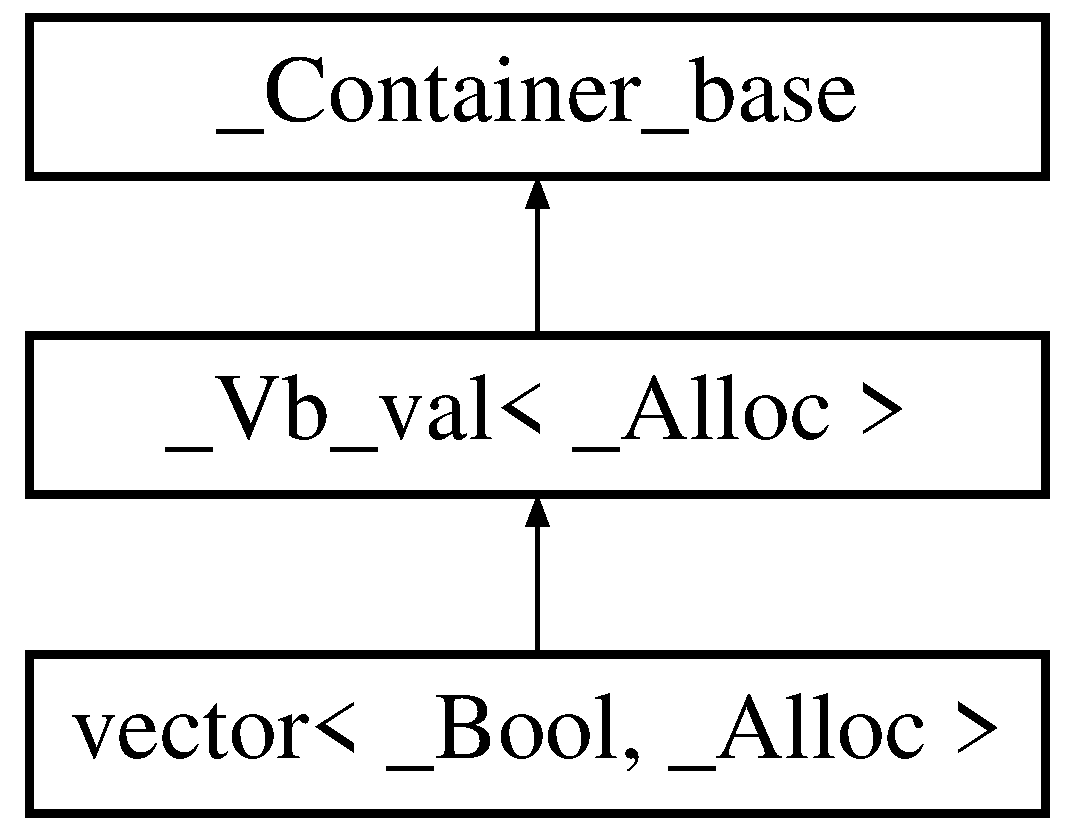
\includegraphics[height=3.000000cm]{classvector_3_01___bool_00_01___alloc_01_4}
\end{center}
\end{figure}
\subsection*{Public Types}
\begin{DoxyCompactItemize}
\item 
typedef \+\_\+\+Alloc\+::size\+\_\+type \hyperlink{classvector_3_01___bool_00_01___alloc_01_4_af9cea187d823373a41b15fea30455e7a}{size\+\_\+type}
\item 
typedef \+\_\+\+Alloc\+::difference\+\_\+type \hyperlink{classvector_3_01___bool_00_01___alloc_01_4_ab724ede91c7a24f8e27c0dca79f10742}{\+\_\+\+Dift}
\item 
typedef \+\_\+\+S\+T\+D \hyperlink{classvector}{vector}$<$ \hyperlink{vector_8h_a1555a2f621ba9ade75bb9ce8bca77144}{\+\_\+\+Vbase}, \\*
typename \+\_\+\+Alloc\+::template \\*
rebind$<$ \hyperlink{vector_8h_a1555a2f621ba9ade75bb9ce8bca77144}{\+\_\+\+Vbase} $>$\+::other $>$ \hyperlink{classvector_3_01___bool_00_01___alloc_01_4_a75194d2d323a8ab90a486691176345f5}{\+\_\+\+Vbtype}
\item 
typedef \+\_\+\+S\+T\+D \hyperlink{classvector}{vector}$<$ \+\_\+\+Bool, \\*
\+\_\+\+Alloc $>$ \hyperlink{classvector_3_01___bool_00_01___alloc_01_4_ada353b682f03c458260a7f7cf361d465}{\+\_\+\+Myt}
\item 
typedef \hyperlink{class___vb__val}{\+\_\+\+Vb\+\_\+val}$<$ \+\_\+\+Alloc $>$ \hyperlink{classvector_3_01___bool_00_01___alloc_01_4_a90abb38ec959ec3cdec7a70765171609}{\+\_\+\+Mybase}
\item 
typedef \hyperlink{classvector_3_01___bool_00_01___alloc_01_4_ab724ede91c7a24f8e27c0dca79f10742}{\+\_\+\+Dift} \hyperlink{classvector_3_01___bool_00_01___alloc_01_4_ada17d1119c13b3e998d89dcec059b2ce}{difference\+\_\+type}
\item 
typedef \+\_\+\+Bool \hyperlink{classvector_3_01___bool_00_01___alloc_01_4_aa52755d5f25533b3a4db77fa17b528a7}{\+\_\+\+Ty}
\item 
typedef \+\_\+\+Alloc \hyperlink{classvector_3_01___bool_00_01___alloc_01_4_a5d383a2381a0b1643f8c2b9618286c95}{allocator\+\_\+type}
\item 
typedef \hyperlink{class___vb__reference}{\+\_\+\+Vb\+\_\+reference}$<$ \+\_\+\+Alloc $>$ \hyperlink{classvector_3_01___bool_00_01___alloc_01_4_afa1a38ae57c26454f265b34ebc302830}{reference}
\item 
typedef bool \hyperlink{classvector_3_01___bool_00_01___alloc_01_4_ab8b5b0a3cc432065c3a9083e11014298}{const\+\_\+reference}
\item 
typedef bool \hyperlink{classvector_3_01___bool_00_01___alloc_01_4_ab9c7e051ec6defeeeb22fa53d3cfca8c}{value\+\_\+type}
\item 
typedef \hyperlink{classvector_3_01___bool_00_01___alloc_01_4_afa1a38ae57c26454f265b34ebc302830}{reference} \hyperlink{classvector_3_01___bool_00_01___alloc_01_4_a22d06114ab3f5ef9677e423f41d99846}{\+\_\+\+Reft}
\item 
typedef \hyperlink{class___vb__const__iterator}{\+\_\+\+Vb\+\_\+const\+\_\+iterator}\\*
$<$ \+\_\+\+Alloc $>$ \hyperlink{classvector_3_01___bool_00_01___alloc_01_4_a79966c86fbbd4dcb38b01eb352633b7e}{const\+\_\+iterator}
\item 
typedef \hyperlink{class___vb__iterator}{\+\_\+\+Vb\+\_\+iterator}$<$ \+\_\+\+Alloc $>$ \hyperlink{classvector_3_01___bool_00_01___alloc_01_4_a151edfa584da275286dbb10b3992940e}{iterator}
\item 
typedef \hyperlink{classvector_3_01___bool_00_01___alloc_01_4_a151edfa584da275286dbb10b3992940e}{iterator} \hyperlink{classvector_3_01___bool_00_01___alloc_01_4_a7694039a51b5a3b856f2c1438d6f5700}{pointer}
\item 
typedef \hyperlink{classvector_3_01___bool_00_01___alloc_01_4_a79966c86fbbd4dcb38b01eb352633b7e}{const\+\_\+iterator} \hyperlink{classvector_3_01___bool_00_01___alloc_01_4_a37c69754c68d037af4ff810352cfefe7}{const\+\_\+pointer}
\item 
typedef \+\_\+\+S\+T\+D \hyperlink{classvector_3_01___bool_00_01___alloc_01_4_a91f49dea5e022761921d459ecd97aef7}{reverse\+\_\+iterator}\\*
$<$ \hyperlink{classvector_3_01___bool_00_01___alloc_01_4_a151edfa584da275286dbb10b3992940e}{iterator} $>$ \hyperlink{classvector_3_01___bool_00_01___alloc_01_4_a91f49dea5e022761921d459ecd97aef7}{reverse\+\_\+iterator}
\item 
typedef \+\_\+\+S\+T\+D \hyperlink{classvector_3_01___bool_00_01___alloc_01_4_a91f49dea5e022761921d459ecd97aef7}{reverse\+\_\+iterator}\\*
$<$ \hyperlink{classvector_3_01___bool_00_01___alloc_01_4_a79966c86fbbd4dcb38b01eb352633b7e}{const\+\_\+iterator} $>$ \hyperlink{classvector_3_01___bool_00_01___alloc_01_4_a519201ff91b19c9cf5f448eee90401d8}{const\+\_\+reverse\+\_\+iterator}
\end{DoxyCompactItemize}
\subsection*{Public Member Functions}
\begin{DoxyCompactItemize}
\item 
\hyperlink{classvector_3_01___bool_00_01___alloc_01_4_afd4c7f3332d8ebdd70049f8a5d262b58}{vector} ()
\item 
\hyperlink{classvector_3_01___bool_00_01___alloc_01_4_ab48c3b5446e5fc35dfe20f58f75813bc}{vector} (const \hyperlink{classvector_3_01___bool_00_01___alloc_01_4_ada353b682f03c458260a7f7cf361d465}{\+\_\+\+Myt} \&\+\_\+\+Right)
\item 
\hyperlink{classvector_3_01___bool_00_01___alloc_01_4_a35a7cae1b0ce66a2cb6efe078d9724ec}{vector} (const \+\_\+\+Alloc \&\+\_\+\+Al)
\item 
\hyperlink{classvector_3_01___bool_00_01___alloc_01_4_ad905fdd366a0d208d5d1691d42062276}{vector} (\hyperlink{class___vb__val_aae6aa10bcd41d235b46f128df1198612}{size\+\_\+type} \+\_\+\+Count, bool \+\_\+\+Val=false)
\item 
\hyperlink{classvector_3_01___bool_00_01___alloc_01_4_a1704244314427d71196810f7464f7a64}{vector} (\hyperlink{class___vb__val_aae6aa10bcd41d235b46f128df1198612}{size\+\_\+type} \+\_\+\+Count, bool \+\_\+\+Val, const \+\_\+\+Alloc \&\+\_\+\+Al)
\item 
{\footnotesize template$<$class \+\_\+\+Iter $>$ }\\\hyperlink{classvector_3_01___bool_00_01___alloc_01_4_a22dd8a5a28d58044c0cf7d3f6afca43f}{vector} (\+\_\+\+Iter \+\_\+\+First, \+\_\+\+Iter \+\_\+\+Last)
\item 
{\footnotesize template$<$class \+\_\+\+Iter $>$ }\\\hyperlink{classvector_3_01___bool_00_01___alloc_01_4_aa63b6633740c58b97313a6b5cf65cece}{vector} (\+\_\+\+Iter \+\_\+\+First, \+\_\+\+Iter \+\_\+\+Last, const \+\_\+\+Alloc \&\+\_\+\+Al)
\item 
{\footnotesize template$<$class \+\_\+\+Iter $>$ }\\void \hyperlink{classvector_3_01___bool_00_01___alloc_01_4_a46790e35a277143c9539d0cb3d3153aa}{\+\_\+\+B\+Construct} (\+\_\+\+Iter \+\_\+\+Count, \+\_\+\+Iter \+\_\+\+Val, \+\_\+\+Int\+\_\+iterator\+\_\+tag)
\item 
{\footnotesize template$<$class \+\_\+\+Iter $>$ }\\void \hyperlink{classvector_3_01___bool_00_01___alloc_01_4_a383643e134283429ec3038cd91252fab}{\+\_\+\+B\+Construct} (\+\_\+\+Iter \+\_\+\+First, \+\_\+\+Iter \+\_\+\+Last, input\+\_\+iterator\+\_\+tag)
\item 
\hyperlink{classvector_3_01___bool_00_01___alloc_01_4_a6e7b1a5180f91465e7a05b719d2881af}{vector} (\hyperlink{classvector_3_01___bool_00_01___alloc_01_4_ada353b682f03c458260a7f7cf361d465}{\+\_\+\+Myt} \&\&\+\_\+\+Right)
\item 
\hyperlink{classvector_3_01___bool_00_01___alloc_01_4_ada353b682f03c458260a7f7cf361d465}{\+\_\+\+Myt} \& \hyperlink{classvector_3_01___bool_00_01___alloc_01_4_a54e6af1534eb6211a811530cce48c5fe}{operator=} (\hyperlink{classvector_3_01___bool_00_01___alloc_01_4_ada353b682f03c458260a7f7cf361d465}{\+\_\+\+Myt} \&\&\+\_\+\+Right)
\item 
void \hyperlink{classvector_3_01___bool_00_01___alloc_01_4_af895ed327cabc0d2d907f7067539114f}{\+\_\+\+Assign\+\_\+rv} (\hyperlink{classvector_3_01___bool_00_01___alloc_01_4_ada353b682f03c458260a7f7cf361d465}{\+\_\+\+Myt} \&\&\+\_\+\+Right)
\item 
void \hyperlink{classvector_3_01___bool_00_01___alloc_01_4_af87782a7d5c33b75008d8a7a68366d50}{swap} (\hyperlink{classvector_3_01___bool_00_01___alloc_01_4_ada353b682f03c458260a7f7cf361d465}{\+\_\+\+Myt} \&\&\+\_\+\+Right)
\item 
\hyperlink{classvector_3_01___bool_00_01___alloc_01_4_a4fbcbd767d7224d231627f91487cac36}{$\sim$vector} ()
\item 
\hyperlink{classvector_3_01___bool_00_01___alloc_01_4_ada353b682f03c458260a7f7cf361d465}{\+\_\+\+Myt} \& \hyperlink{classvector_3_01___bool_00_01___alloc_01_4_a755ced058465a272e916353108868644}{operator=} (const \hyperlink{classvector_3_01___bool_00_01___alloc_01_4_ada353b682f03c458260a7f7cf361d465}{\+\_\+\+Myt} \&\+\_\+\+Right)
\item 
void \hyperlink{classvector_3_01___bool_00_01___alloc_01_4_a602a98fa3dc182d965c7727fdc2c868d}{reserve} (\hyperlink{class___vb__val_aae6aa10bcd41d235b46f128df1198612}{size\+\_\+type} \+\_\+\+Count)
\item 
\hyperlink{class___vb__val_aae6aa10bcd41d235b46f128df1198612}{size\+\_\+type} \hyperlink{classvector_3_01___bool_00_01___alloc_01_4_ad2ef8ef71dc251f26c8fd9fb93cbd742}{capacity} () const 
\item 
\hyperlink{classvector_3_01___bool_00_01___alloc_01_4_a151edfa584da275286dbb10b3992940e}{iterator} \hyperlink{classvector_3_01___bool_00_01___alloc_01_4_a19dd2102d2fc4ec2945aa6861e79680a}{begin} ()
\item 
\hyperlink{classvector_3_01___bool_00_01___alloc_01_4_a79966c86fbbd4dcb38b01eb352633b7e}{const\+\_\+iterator} \hyperlink{classvector_3_01___bool_00_01___alloc_01_4_a3fa8ff276105c7cc0a72e956f33fc24c}{begin} () const 
\item 
\hyperlink{classvector_3_01___bool_00_01___alloc_01_4_a151edfa584da275286dbb10b3992940e}{iterator} \hyperlink{classvector_3_01___bool_00_01___alloc_01_4_a7d4fa5f8713cf4580ccd3cfe62cafb44}{end} ()
\item 
\hyperlink{classvector_3_01___bool_00_01___alloc_01_4_a79966c86fbbd4dcb38b01eb352633b7e}{const\+\_\+iterator} \hyperlink{classvector_3_01___bool_00_01___alloc_01_4_a16fdcc2b68caa2fd00bac54ff1c72b2a}{end} () const 
\item 
\hyperlink{classvector_3_01___bool_00_01___alloc_01_4_a151edfa584da275286dbb10b3992940e}{iterator} \hyperlink{classvector_3_01___bool_00_01___alloc_01_4_a9a3da0f9aafe46dc07395943604ac685}{\+\_\+\+Make\+\_\+iter} (\hyperlink{classvector_3_01___bool_00_01___alloc_01_4_a79966c86fbbd4dcb38b01eb352633b7e}{const\+\_\+iterator} \+\_\+\+Where)
\item 
\hyperlink{classvector_3_01___bool_00_01___alloc_01_4_a91f49dea5e022761921d459ecd97aef7}{reverse\+\_\+iterator} \hyperlink{classvector_3_01___bool_00_01___alloc_01_4_a04dc7e9633d02d2d5edf6cd810dc7d6b}{rbegin} ()
\item 
\hyperlink{classvector_3_01___bool_00_01___alloc_01_4_a519201ff91b19c9cf5f448eee90401d8}{const\+\_\+reverse\+\_\+iterator} \hyperlink{classvector_3_01___bool_00_01___alloc_01_4_a48c2430ff4a01de93be7b188faad3d44}{rbegin} () const 
\item 
\hyperlink{classvector_3_01___bool_00_01___alloc_01_4_a91f49dea5e022761921d459ecd97aef7}{reverse\+\_\+iterator} \hyperlink{classvector_3_01___bool_00_01___alloc_01_4_a4bdfc2490f8639303fe1597b626c5d6a}{rend} ()
\item 
\hyperlink{classvector_3_01___bool_00_01___alloc_01_4_a519201ff91b19c9cf5f448eee90401d8}{const\+\_\+reverse\+\_\+iterator} \hyperlink{classvector_3_01___bool_00_01___alloc_01_4_aa2c6f488376d8f743feed2028b7fa86c}{rend} () const 
\item 
void \hyperlink{classvector_3_01___bool_00_01___alloc_01_4_abbc62c8941c477f57326db9fb15ef097}{resize} (\hyperlink{class___vb__val_aae6aa10bcd41d235b46f128df1198612}{size\+\_\+type} \+\_\+\+Newsize, bool \+\_\+\+Val=false)
\item 
\hyperlink{class___vb__val_aae6aa10bcd41d235b46f128df1198612}{size\+\_\+type} \hyperlink{classvector_3_01___bool_00_01___alloc_01_4_a70977d2def0375c86b653e9c0596546a}{size} () const 
\item 
\hyperlink{class___vb__val_aae6aa10bcd41d235b46f128df1198612}{size\+\_\+type} \hyperlink{classvector_3_01___bool_00_01___alloc_01_4_a15e355b8e1a8998ac9a000ab98c71b46}{max\+\_\+size} () const 
\item 
bool \hyperlink{classvector_3_01___bool_00_01___alloc_01_4_aeaa21a18649efe4485a6e789f15252bb}{empty} () const 
\item 
\+\_\+\+Alloc \hyperlink{classvector_3_01___bool_00_01___alloc_01_4_ab87610196de7a6abe8f5ea77c1a54c49}{get\+\_\+allocator} () const 
\item 
\hyperlink{classvector_3_01___bool_00_01___alloc_01_4_ab8b5b0a3cc432065c3a9083e11014298}{const\+\_\+reference} \hyperlink{classvector_3_01___bool_00_01___alloc_01_4_a43e08421e6570b0a9aa3a1f1b355cb81}{at} (\hyperlink{class___vb__val_aae6aa10bcd41d235b46f128df1198612}{size\+\_\+type} \+\_\+\+Off) const 
\item 
\hyperlink{classvector_3_01___bool_00_01___alloc_01_4_afa1a38ae57c26454f265b34ebc302830}{reference} \hyperlink{classvector_3_01___bool_00_01___alloc_01_4_accb557af39c9e744de03316d2f15becb}{at} (\hyperlink{class___vb__val_aae6aa10bcd41d235b46f128df1198612}{size\+\_\+type} \+\_\+\+Off)
\item 
\hyperlink{classvector_3_01___bool_00_01___alloc_01_4_ab8b5b0a3cc432065c3a9083e11014298}{const\+\_\+reference} \hyperlink{classvector_3_01___bool_00_01___alloc_01_4_aab197769e540b7753427368a41eeda76}{operator\mbox{[}$\,$\mbox{]}} (\hyperlink{class___vb__val_aae6aa10bcd41d235b46f128df1198612}{size\+\_\+type} \+\_\+\+Off) const 
\item 
\hyperlink{classvector_3_01___bool_00_01___alloc_01_4_afa1a38ae57c26454f265b34ebc302830}{reference} \hyperlink{classvector_3_01___bool_00_01___alloc_01_4_a6b7d2a9a35aa58b15982aad8ee1c4e06}{operator\mbox{[}$\,$\mbox{]}} (\hyperlink{class___vb__val_aae6aa10bcd41d235b46f128df1198612}{size\+\_\+type} \+\_\+\+Off)
\item 
\hyperlink{classvector_3_01___bool_00_01___alloc_01_4_afa1a38ae57c26454f265b34ebc302830}{reference} \hyperlink{classvector_3_01___bool_00_01___alloc_01_4_a65847634e6121fad1d886b0baa6ab5bc}{front} ()
\item 
\hyperlink{classvector_3_01___bool_00_01___alloc_01_4_ab8b5b0a3cc432065c3a9083e11014298}{const\+\_\+reference} \hyperlink{classvector_3_01___bool_00_01___alloc_01_4_a9a0aa91d0d91abd2927fee133ef78540}{front} () const 
\item 
\hyperlink{classvector_3_01___bool_00_01___alloc_01_4_afa1a38ae57c26454f265b34ebc302830}{reference} \hyperlink{classvector_3_01___bool_00_01___alloc_01_4_a00542b2998425061ccfceff36ce0b8ba}{back} ()
\item 
\hyperlink{classvector_3_01___bool_00_01___alloc_01_4_ab8b5b0a3cc432065c3a9083e11014298}{const\+\_\+reference} \hyperlink{classvector_3_01___bool_00_01___alloc_01_4_aa568ec056494a24a9fa2fb1e633a8262}{back} () const 
\item 
void \hyperlink{classvector_3_01___bool_00_01___alloc_01_4_a51a8feb75ebb3f949e5dde1c68ac9087}{push\+\_\+back} (bool \+\_\+\+Val)
\item 
void \hyperlink{classvector_3_01___bool_00_01___alloc_01_4_a1b4db666e591e12af3411573301564cc}{pop\+\_\+back} ()
\item 
{\footnotesize template$<$class \+\_\+\+Iter $>$ }\\void \hyperlink{classvector_3_01___bool_00_01___alloc_01_4_a517c1fadf919ec08fea26b4361773e31}{assign} (\+\_\+\+Iter \+\_\+\+First, \+\_\+\+Iter \+\_\+\+Last)
\item 
{\footnotesize template$<$class \+\_\+\+Iter $>$ }\\void \hyperlink{classvector_3_01___bool_00_01___alloc_01_4_a10b1e50fcac7063a74a29346039fbacc}{\+\_\+\+Assign} (\+\_\+\+Iter \+\_\+\+Count, \+\_\+\+Iter \+\_\+\+Val, \+\_\+\+Int\+\_\+iterator\+\_\+tag)
\item 
{\footnotesize template$<$class \+\_\+\+Iter $>$ }\\void \hyperlink{classvector_3_01___bool_00_01___alloc_01_4_abe6c2b97561d683aea1bad2af1ca4188}{\+\_\+\+Assign} (\+\_\+\+Iter \+\_\+\+First, \+\_\+\+Iter \+\_\+\+Last, input\+\_\+iterator\+\_\+tag)
\item 
void \hyperlink{classvector_3_01___bool_00_01___alloc_01_4_af56bc3099f1e07525e1941cc65852291}{assign} (\hyperlink{class___vb__val_aae6aa10bcd41d235b46f128df1198612}{size\+\_\+type} \+\_\+\+Count, bool \+\_\+\+Val)
\item 
\hyperlink{classvector_3_01___bool_00_01___alloc_01_4_a151edfa584da275286dbb10b3992940e}{iterator} \hyperlink{classvector_3_01___bool_00_01___alloc_01_4_a2242f90709958c4e134ddb35eafaa1f3}{insert} (\hyperlink{classvector_3_01___bool_00_01___alloc_01_4_a79966c86fbbd4dcb38b01eb352633b7e}{const\+\_\+iterator} \+\_\+\+Where, bool \+\_\+\+Val)
\item 
void \hyperlink{classvector_3_01___bool_00_01___alloc_01_4_a802c95a85e7f32ff18e90b3dcca34ef1}{insert} (\hyperlink{classvector_3_01___bool_00_01___alloc_01_4_a79966c86fbbd4dcb38b01eb352633b7e}{const\+\_\+iterator} \+\_\+\+Where, \hyperlink{class___vb__val_aae6aa10bcd41d235b46f128df1198612}{size\+\_\+type} \+\_\+\+Count, bool \+\_\+\+Val)
\item 
{\footnotesize template$<$class \+\_\+\+Iter $>$ }\\void \hyperlink{classvector_3_01___bool_00_01___alloc_01_4_a4b631226adebbfc2408a790b9fc0afea}{insert} (\hyperlink{classvector_3_01___bool_00_01___alloc_01_4_a79966c86fbbd4dcb38b01eb352633b7e}{const\+\_\+iterator} \+\_\+\+Where, \+\_\+\+Iter \+\_\+\+First, \+\_\+\+Iter \+\_\+\+Last)
\item 
{\footnotesize template$<$class \+\_\+\+Iter $>$ }\\void \hyperlink{classvector_3_01___bool_00_01___alloc_01_4_a58c0225a996079969cef68e2dbe76204}{\+\_\+\+Insert} (\hyperlink{classvector_3_01___bool_00_01___alloc_01_4_a79966c86fbbd4dcb38b01eb352633b7e}{const\+\_\+iterator} \+\_\+\+Where, \+\_\+\+Iter \+\_\+\+Count, \+\_\+\+Iter \+\_\+\+Val, \+\_\+\+Int\+\_\+iterator\+\_\+tag)
\item 
{\footnotesize template$<$class \+\_\+\+Iter $>$ }\\void \hyperlink{classvector_3_01___bool_00_01___alloc_01_4_aa8aa01469992b5f7874d00345a5ce292}{\+\_\+\+Insert} (\hyperlink{classvector_3_01___bool_00_01___alloc_01_4_a79966c86fbbd4dcb38b01eb352633b7e}{const\+\_\+iterator} \+\_\+\+Where, \+\_\+\+Iter \+\_\+\+First, \+\_\+\+Iter \+\_\+\+Last, input\+\_\+iterator\+\_\+tag)
\item 
{\footnotesize template$<$class \+\_\+\+Iter $>$ }\\void \hyperlink{classvector_3_01___bool_00_01___alloc_01_4_a8a456974f19919fbfbab89c9bfdbe5c6}{\+\_\+\+Insert} (\hyperlink{classvector_3_01___bool_00_01___alloc_01_4_a79966c86fbbd4dcb38b01eb352633b7e}{const\+\_\+iterator} \+\_\+\+Where, \+\_\+\+Iter \+\_\+\+First, \+\_\+\+Iter \+\_\+\+Last, forward\+\_\+iterator\+\_\+tag)
\item 
\hyperlink{classvector_3_01___bool_00_01___alloc_01_4_a151edfa584da275286dbb10b3992940e}{iterator} \hyperlink{classvector_3_01___bool_00_01___alloc_01_4_a1963ca8c8a65a3acf4510d72aa016874}{erase} (\hyperlink{classvector_3_01___bool_00_01___alloc_01_4_a79966c86fbbd4dcb38b01eb352633b7e}{const\+\_\+iterator} \+\_\+\+Where\+\_\+arg)
\item 
\hyperlink{classvector_3_01___bool_00_01___alloc_01_4_a151edfa584da275286dbb10b3992940e}{iterator} \hyperlink{classvector_3_01___bool_00_01___alloc_01_4_a2494531f4ab150b2853a991e5e050de0}{erase} (\hyperlink{classvector_3_01___bool_00_01___alloc_01_4_a79966c86fbbd4dcb38b01eb352633b7e}{const\+\_\+iterator} \+\_\+\+First\+\_\+arg, \hyperlink{classvector_3_01___bool_00_01___alloc_01_4_a79966c86fbbd4dcb38b01eb352633b7e}{const\+\_\+iterator} \+\_\+\+Last\+\_\+arg)
\item 
void \hyperlink{classvector_3_01___bool_00_01___alloc_01_4_a5a2b6108043801ce6f7c47d4010dc481}{clear} ()
\item 
void \hyperlink{classvector_3_01___bool_00_01___alloc_01_4_aa99d462f5e2c91cb931bb387a72ef3ee}{flip} ()
\item 
void \hyperlink{classvector_3_01___bool_00_01___alloc_01_4_a5bd5ce713d5e68299b8fe3e8d58d2814}{swap} (\hyperlink{classvector_3_01___bool_00_01___alloc_01_4_ada353b682f03c458260a7f7cf361d465}{\+\_\+\+Myt} \&\+\_\+\+Right)
\item 
void \hyperlink{classvector_3_01___bool_00_01___alloc_01_4_acd24861948baa50a924b437f24b82ae8}{\+\_\+\+Assign\+\_\+n} (\hyperlink{class___vb__val_aae6aa10bcd41d235b46f128df1198612}{size\+\_\+type} \+\_\+\+Count, bool \+\_\+\+Val)
\item 
void \hyperlink{classvector_3_01___bool_00_01___alloc_01_4_aca042831876c7a7d02a54f9d63cf7276}{\+\_\+\+Insert\+\_\+n} (\hyperlink{classvector_3_01___bool_00_01___alloc_01_4_a79966c86fbbd4dcb38b01eb352633b7e}{const\+\_\+iterator} \+\_\+\+Where, \hyperlink{class___vb__val_aae6aa10bcd41d235b46f128df1198612}{size\+\_\+type} \+\_\+\+Count, bool \+\_\+\+Val)
\item 
\hyperlink{class___vb__val_aae6aa10bcd41d235b46f128df1198612}{size\+\_\+type} \hyperlink{classvector_3_01___bool_00_01___alloc_01_4_a8ef1811e956700dd89f3d915a2007238}{\+\_\+\+Insert\+\_\+x} (\hyperlink{classvector_3_01___bool_00_01___alloc_01_4_a79966c86fbbd4dcb38b01eb352633b7e}{const\+\_\+iterator} \+\_\+\+Where, \hyperlink{class___vb__val_aae6aa10bcd41d235b46f128df1198612}{size\+\_\+type} \+\_\+\+Count)
\item 
void \hyperlink{classvector_3_01___bool_00_01___alloc_01_4_ae8604e2d46563fbfa2ed79bbba975559}{\+\_\+\+Orphan\+\_\+range} (\hyperlink{class___vb__val_aae6aa10bcd41d235b46f128df1198612}{size\+\_\+type}, \hyperlink{class___vb__val_aae6aa10bcd41d235b46f128df1198612}{size\+\_\+type}) const 
\item 
void \hyperlink{classvector_3_01___bool_00_01___alloc_01_4_a619aafe2c9f87463926dd5d7f62aa917}{\+\_\+\+Trim} (\hyperlink{class___vb__val_aae6aa10bcd41d235b46f128df1198612}{size\+\_\+type} \+\_\+\+Size)
\item 
\hyperlink{classvector_3_01___bool_00_01___alloc_01_4_a778459dd62f998a3b34468c166144283}{\+\_\+\+\_\+declspec} (noreturn) void \+\_\+\+Xlen() const 
\item 
\hyperlink{classvector_3_01___bool_00_01___alloc_01_4_a714fa9f6a856d9d7ced85aea5a2c7edc}{\+\_\+\+\_\+declspec} (noreturn) void \+\_\+\+Xran() const 
\end{DoxyCompactItemize}
\subsection*{Static Public Member Functions}
\begin{DoxyCompactItemize}
\item 
static void \hyperlink{classvector_3_01___bool_00_01___alloc_01_4_aa38ac97b69b2053641fd95680200ed2e}{swap} (\hyperlink{classvector_3_01___bool_00_01___alloc_01_4_afa1a38ae57c26454f265b34ebc302830}{reference} \+\_\+\+Left, \hyperlink{classvector_3_01___bool_00_01___alloc_01_4_afa1a38ae57c26454f265b34ebc302830}{reference} \+\_\+\+Right)
\end{DoxyCompactItemize}
\subsection*{Static Public Attributes}
\begin{DoxyCompactItemize}
\item 
static const int \hyperlink{classvector_3_01___bool_00_01___alloc_01_4_a225e72f3099206a41937bb30e5aaf9ed}{\+\_\+\+V\+B\+I\+T\+S} = \+\_\+\+S\+T\+D \+\_\+\+V\+B\+I\+T\+S
\end{DoxyCompactItemize}
\subsection*{Additional Inherited Members}


\subsection{Detailed Description}
\subsubsection*{template$<$class \+\_\+\+Alloc$>$class vector$<$ \+\_\+\+Bool, \+\_\+\+Alloc $>$}



Definition at line 2063 of file vector.\+h.



\subsection{Member Typedef Documentation}
\hypertarget{classvector_3_01___bool_00_01___alloc_01_4_ab724ede91c7a24f8e27c0dca79f10742}{\index{vector$<$ \+\_\+\+Bool, \+\_\+\+Alloc $>$@{vector$<$ \+\_\+\+Bool, \+\_\+\+Alloc $>$}!\+\_\+\+Dift@{\+\_\+\+Dift}}
\index{\+\_\+\+Dift@{\+\_\+\+Dift}!vector$<$ \+\_\+\+Bool, \+\_\+\+Alloc $>$@{vector$<$ \+\_\+\+Bool, \+\_\+\+Alloc $>$}}
\subsubsection[{\+\_\+\+Dift}]{\setlength{\rightskip}{0pt plus 5cm}template$<$class \+\_\+\+Alloc $>$ typedef \+\_\+\+Alloc\+::difference\+\_\+type {\bf vector}$<$ \+\_\+\+Bool, \+\_\+\+Alloc $>$\+::{\bf \+\_\+\+Dift}}}\label{classvector_3_01___bool_00_01___alloc_01_4_ab724ede91c7a24f8e27c0dca79f10742}


Definition at line 2068 of file vector.\+h.

\hypertarget{classvector_3_01___bool_00_01___alloc_01_4_a90abb38ec959ec3cdec7a70765171609}{\index{vector$<$ \+\_\+\+Bool, \+\_\+\+Alloc $>$@{vector$<$ \+\_\+\+Bool, \+\_\+\+Alloc $>$}!\+\_\+\+Mybase@{\+\_\+\+Mybase}}
\index{\+\_\+\+Mybase@{\+\_\+\+Mybase}!vector$<$ \+\_\+\+Bool, \+\_\+\+Alloc $>$@{vector$<$ \+\_\+\+Bool, \+\_\+\+Alloc $>$}}
\subsubsection[{\+\_\+\+Mybase}]{\setlength{\rightskip}{0pt plus 5cm}template$<$class \+\_\+\+Alloc $>$ typedef {\bf \+\_\+\+Vb\+\_\+val}$<$\+\_\+\+Alloc$>$ {\bf vector}$<$ \+\_\+\+Bool, \+\_\+\+Alloc $>$\+::{\bf \+\_\+\+Mybase}}}\label{classvector_3_01___bool_00_01___alloc_01_4_a90abb38ec959ec3cdec7a70765171609}


Definition at line 2074 of file vector.\+h.

\hypertarget{classvector_3_01___bool_00_01___alloc_01_4_ada353b682f03c458260a7f7cf361d465}{\index{vector$<$ \+\_\+\+Bool, \+\_\+\+Alloc $>$@{vector$<$ \+\_\+\+Bool, \+\_\+\+Alloc $>$}!\+\_\+\+Myt@{\+\_\+\+Myt}}
\index{\+\_\+\+Myt@{\+\_\+\+Myt}!vector$<$ \+\_\+\+Bool, \+\_\+\+Alloc $>$@{vector$<$ \+\_\+\+Bool, \+\_\+\+Alloc $>$}}
\subsubsection[{\+\_\+\+Myt}]{\setlength{\rightskip}{0pt plus 5cm}template$<$class \+\_\+\+Alloc $>$ typedef \+\_\+\+S\+T\+D {\bf vector}$<$\+\_\+\+Bool, \+\_\+\+Alloc$>$ {\bf vector}$<$ \+\_\+\+Bool, \+\_\+\+Alloc $>$\+::{\bf \+\_\+\+Myt}}}\label{classvector_3_01___bool_00_01___alloc_01_4_ada353b682f03c458260a7f7cf361d465}


Definition at line 2073 of file vector.\+h.

\hypertarget{classvector_3_01___bool_00_01___alloc_01_4_a22d06114ab3f5ef9677e423f41d99846}{\index{vector$<$ \+\_\+\+Bool, \+\_\+\+Alloc $>$@{vector$<$ \+\_\+\+Bool, \+\_\+\+Alloc $>$}!\+\_\+\+Reft@{\+\_\+\+Reft}}
\index{\+\_\+\+Reft@{\+\_\+\+Reft}!vector$<$ \+\_\+\+Bool, \+\_\+\+Alloc $>$@{vector$<$ \+\_\+\+Bool, \+\_\+\+Alloc $>$}}
\subsubsection[{\+\_\+\+Reft}]{\setlength{\rightskip}{0pt plus 5cm}template$<$class \+\_\+\+Alloc $>$ typedef {\bf reference} {\bf vector}$<$ \+\_\+\+Bool, \+\_\+\+Alloc $>$\+::{\bf \+\_\+\+Reft}}}\label{classvector_3_01___bool_00_01___alloc_01_4_a22d06114ab3f5ef9677e423f41d99846}


Definition at line 2084 of file vector.\+h.

\hypertarget{classvector_3_01___bool_00_01___alloc_01_4_aa52755d5f25533b3a4db77fa17b528a7}{\index{vector$<$ \+\_\+\+Bool, \+\_\+\+Alloc $>$@{vector$<$ \+\_\+\+Bool, \+\_\+\+Alloc $>$}!\+\_\+\+Ty@{\+\_\+\+Ty}}
\index{\+\_\+\+Ty@{\+\_\+\+Ty}!vector$<$ \+\_\+\+Bool, \+\_\+\+Alloc $>$@{vector$<$ \+\_\+\+Bool, \+\_\+\+Alloc $>$}}
\subsubsection[{\+\_\+\+Ty}]{\setlength{\rightskip}{0pt plus 5cm}template$<$class \+\_\+\+Alloc $>$ typedef \+\_\+\+Bool {\bf vector}$<$ \+\_\+\+Bool, \+\_\+\+Alloc $>$\+::{\bf \+\_\+\+Ty}}}\label{classvector_3_01___bool_00_01___alloc_01_4_aa52755d5f25533b3a4db77fa17b528a7}


Definition at line 2077 of file vector.\+h.

\hypertarget{classvector_3_01___bool_00_01___alloc_01_4_a75194d2d323a8ab90a486691176345f5}{\index{vector$<$ \+\_\+\+Bool, \+\_\+\+Alloc $>$@{vector$<$ \+\_\+\+Bool, \+\_\+\+Alloc $>$}!\+\_\+\+Vbtype@{\+\_\+\+Vbtype}}
\index{\+\_\+\+Vbtype@{\+\_\+\+Vbtype}!vector$<$ \+\_\+\+Bool, \+\_\+\+Alloc $>$@{vector$<$ \+\_\+\+Bool, \+\_\+\+Alloc $>$}}
\subsubsection[{\+\_\+\+Vbtype}]{\setlength{\rightskip}{0pt plus 5cm}template$<$class \+\_\+\+Alloc $>$ typedef \+\_\+\+S\+T\+D {\bf vector}$<${\bf \+\_\+\+Vbase}, typename \+\_\+\+Alloc\+::template rebind$<${\bf \+\_\+\+Vbase}$>$\+::other$>$ {\bf vector}$<$ \+\_\+\+Bool, \+\_\+\+Alloc $>$\+::{\bf \+\_\+\+Vbtype}}}\label{classvector_3_01___bool_00_01___alloc_01_4_a75194d2d323a8ab90a486691176345f5}


Definition at line 2071 of file vector.\+h.

\hypertarget{classvector_3_01___bool_00_01___alloc_01_4_a5d383a2381a0b1643f8c2b9618286c95}{\index{vector$<$ \+\_\+\+Bool, \+\_\+\+Alloc $>$@{vector$<$ \+\_\+\+Bool, \+\_\+\+Alloc $>$}!allocator\+\_\+type@{allocator\+\_\+type}}
\index{allocator\+\_\+type@{allocator\+\_\+type}!vector$<$ \+\_\+\+Bool, \+\_\+\+Alloc $>$@{vector$<$ \+\_\+\+Bool, \+\_\+\+Alloc $>$}}
\subsubsection[{allocator\+\_\+type}]{\setlength{\rightskip}{0pt plus 5cm}template$<$class \+\_\+\+Alloc $>$ typedef \+\_\+\+Alloc {\bf vector}$<$ \+\_\+\+Bool, \+\_\+\+Alloc $>$\+::{\bf allocator\+\_\+type}}}\label{classvector_3_01___bool_00_01___alloc_01_4_a5d383a2381a0b1643f8c2b9618286c95}


Definition at line 2078 of file vector.\+h.

\hypertarget{classvector_3_01___bool_00_01___alloc_01_4_a79966c86fbbd4dcb38b01eb352633b7e}{\index{vector$<$ \+\_\+\+Bool, \+\_\+\+Alloc $>$@{vector$<$ \+\_\+\+Bool, \+\_\+\+Alloc $>$}!const\+\_\+iterator@{const\+\_\+iterator}}
\index{const\+\_\+iterator@{const\+\_\+iterator}!vector$<$ \+\_\+\+Bool, \+\_\+\+Alloc $>$@{vector$<$ \+\_\+\+Bool, \+\_\+\+Alloc $>$}}
\subsubsection[{const\+\_\+iterator}]{\setlength{\rightskip}{0pt plus 5cm}template$<$class \+\_\+\+Alloc $>$ typedef {\bf \+\_\+\+Vb\+\_\+const\+\_\+iterator}$<$\+\_\+\+Alloc$>$ {\bf vector}$<$ \+\_\+\+Bool, \+\_\+\+Alloc $>$\+::{\bf const\+\_\+iterator}}}\label{classvector_3_01___bool_00_01___alloc_01_4_a79966c86fbbd4dcb38b01eb352633b7e}


Definition at line 2085 of file vector.\+h.

\hypertarget{classvector_3_01___bool_00_01___alloc_01_4_a37c69754c68d037af4ff810352cfefe7}{\index{vector$<$ \+\_\+\+Bool, \+\_\+\+Alloc $>$@{vector$<$ \+\_\+\+Bool, \+\_\+\+Alloc $>$}!const\+\_\+pointer@{const\+\_\+pointer}}
\index{const\+\_\+pointer@{const\+\_\+pointer}!vector$<$ \+\_\+\+Bool, \+\_\+\+Alloc $>$@{vector$<$ \+\_\+\+Bool, \+\_\+\+Alloc $>$}}
\subsubsection[{const\+\_\+pointer}]{\setlength{\rightskip}{0pt plus 5cm}template$<$class \+\_\+\+Alloc $>$ typedef {\bf const\+\_\+iterator} {\bf vector}$<$ \+\_\+\+Bool, \+\_\+\+Alloc $>$\+::{\bf const\+\_\+pointer}}}\label{classvector_3_01___bool_00_01___alloc_01_4_a37c69754c68d037af4ff810352cfefe7}


Definition at line 2089 of file vector.\+h.

\hypertarget{classvector_3_01___bool_00_01___alloc_01_4_ab8b5b0a3cc432065c3a9083e11014298}{\index{vector$<$ \+\_\+\+Bool, \+\_\+\+Alloc $>$@{vector$<$ \+\_\+\+Bool, \+\_\+\+Alloc $>$}!const\+\_\+reference@{const\+\_\+reference}}
\index{const\+\_\+reference@{const\+\_\+reference}!vector$<$ \+\_\+\+Bool, \+\_\+\+Alloc $>$@{vector$<$ \+\_\+\+Bool, \+\_\+\+Alloc $>$}}
\subsubsection[{const\+\_\+reference}]{\setlength{\rightskip}{0pt plus 5cm}template$<$class \+\_\+\+Alloc $>$ typedef bool {\bf vector}$<$ \+\_\+\+Bool, \+\_\+\+Alloc $>$\+::{\bf const\+\_\+reference}}}\label{classvector_3_01___bool_00_01___alloc_01_4_ab8b5b0a3cc432065c3a9083e11014298}


Definition at line 2081 of file vector.\+h.

\hypertarget{classvector_3_01___bool_00_01___alloc_01_4_a519201ff91b19c9cf5f448eee90401d8}{\index{vector$<$ \+\_\+\+Bool, \+\_\+\+Alloc $>$@{vector$<$ \+\_\+\+Bool, \+\_\+\+Alloc $>$}!const\+\_\+reverse\+\_\+iterator@{const\+\_\+reverse\+\_\+iterator}}
\index{const\+\_\+reverse\+\_\+iterator@{const\+\_\+reverse\+\_\+iterator}!vector$<$ \+\_\+\+Bool, \+\_\+\+Alloc $>$@{vector$<$ \+\_\+\+Bool, \+\_\+\+Alloc $>$}}
\subsubsection[{const\+\_\+reverse\+\_\+iterator}]{\setlength{\rightskip}{0pt plus 5cm}template$<$class \+\_\+\+Alloc $>$ typedef \+\_\+\+S\+T\+D {\bf reverse\+\_\+iterator}$<${\bf const\+\_\+iterator}$>$ {\bf vector}$<$ \+\_\+\+Bool, \+\_\+\+Alloc $>$\+::{\bf const\+\_\+reverse\+\_\+iterator}}}\label{classvector_3_01___bool_00_01___alloc_01_4_a519201ff91b19c9cf5f448eee90401d8}


Definition at line 2091 of file vector.\+h.

\hypertarget{classvector_3_01___bool_00_01___alloc_01_4_ada17d1119c13b3e998d89dcec059b2ce}{\index{vector$<$ \+\_\+\+Bool, \+\_\+\+Alloc $>$@{vector$<$ \+\_\+\+Bool, \+\_\+\+Alloc $>$}!difference\+\_\+type@{difference\+\_\+type}}
\index{difference\+\_\+type@{difference\+\_\+type}!vector$<$ \+\_\+\+Bool, \+\_\+\+Alloc $>$@{vector$<$ \+\_\+\+Bool, \+\_\+\+Alloc $>$}}
\subsubsection[{difference\+\_\+type}]{\setlength{\rightskip}{0pt plus 5cm}template$<$class \+\_\+\+Alloc $>$ typedef {\bf \+\_\+\+Dift} {\bf vector}$<$ \+\_\+\+Bool, \+\_\+\+Alloc $>$\+::{\bf difference\+\_\+type}}}\label{classvector_3_01___bool_00_01___alloc_01_4_ada17d1119c13b3e998d89dcec059b2ce}


Definition at line 2076 of file vector.\+h.

\hypertarget{classvector_3_01___bool_00_01___alloc_01_4_a151edfa584da275286dbb10b3992940e}{\index{vector$<$ \+\_\+\+Bool, \+\_\+\+Alloc $>$@{vector$<$ \+\_\+\+Bool, \+\_\+\+Alloc $>$}!iterator@{iterator}}
\index{iterator@{iterator}!vector$<$ \+\_\+\+Bool, \+\_\+\+Alloc $>$@{vector$<$ \+\_\+\+Bool, \+\_\+\+Alloc $>$}}
\subsubsection[{iterator}]{\setlength{\rightskip}{0pt plus 5cm}template$<$class \+\_\+\+Alloc $>$ typedef {\bf \+\_\+\+Vb\+\_\+iterator}$<$\+\_\+\+Alloc$>$ {\bf vector}$<$ \+\_\+\+Bool, \+\_\+\+Alloc $>$\+::{\bf iterator}}}\label{classvector_3_01___bool_00_01___alloc_01_4_a151edfa584da275286dbb10b3992940e}


Definition at line 2086 of file vector.\+h.

\hypertarget{classvector_3_01___bool_00_01___alloc_01_4_a7694039a51b5a3b856f2c1438d6f5700}{\index{vector$<$ \+\_\+\+Bool, \+\_\+\+Alloc $>$@{vector$<$ \+\_\+\+Bool, \+\_\+\+Alloc $>$}!pointer@{pointer}}
\index{pointer@{pointer}!vector$<$ \+\_\+\+Bool, \+\_\+\+Alloc $>$@{vector$<$ \+\_\+\+Bool, \+\_\+\+Alloc $>$}}
\subsubsection[{pointer}]{\setlength{\rightskip}{0pt plus 5cm}template$<$class \+\_\+\+Alloc $>$ typedef {\bf iterator} {\bf vector}$<$ \+\_\+\+Bool, \+\_\+\+Alloc $>$\+::{\bf pointer}}}\label{classvector_3_01___bool_00_01___alloc_01_4_a7694039a51b5a3b856f2c1438d6f5700}


Definition at line 2088 of file vector.\+h.

\hypertarget{classvector_3_01___bool_00_01___alloc_01_4_afa1a38ae57c26454f265b34ebc302830}{\index{vector$<$ \+\_\+\+Bool, \+\_\+\+Alloc $>$@{vector$<$ \+\_\+\+Bool, \+\_\+\+Alloc $>$}!reference@{reference}}
\index{reference@{reference}!vector$<$ \+\_\+\+Bool, \+\_\+\+Alloc $>$@{vector$<$ \+\_\+\+Bool, \+\_\+\+Alloc $>$}}
\subsubsection[{reference}]{\setlength{\rightskip}{0pt plus 5cm}template$<$class \+\_\+\+Alloc $>$ typedef {\bf \+\_\+\+Vb\+\_\+reference}$<$\+\_\+\+Alloc$>$ {\bf vector}$<$ \+\_\+\+Bool, \+\_\+\+Alloc $>$\+::{\bf reference}}}\label{classvector_3_01___bool_00_01___alloc_01_4_afa1a38ae57c26454f265b34ebc302830}


Definition at line 2080 of file vector.\+h.

\hypertarget{classvector_3_01___bool_00_01___alloc_01_4_a91f49dea5e022761921d459ecd97aef7}{\index{vector$<$ \+\_\+\+Bool, \+\_\+\+Alloc $>$@{vector$<$ \+\_\+\+Bool, \+\_\+\+Alloc $>$}!reverse\+\_\+iterator@{reverse\+\_\+iterator}}
\index{reverse\+\_\+iterator@{reverse\+\_\+iterator}!vector$<$ \+\_\+\+Bool, \+\_\+\+Alloc $>$@{vector$<$ \+\_\+\+Bool, \+\_\+\+Alloc $>$}}
\subsubsection[{reverse\+\_\+iterator}]{\setlength{\rightskip}{0pt plus 5cm}template$<$class \+\_\+\+Alloc $>$ typedef \+\_\+\+S\+T\+D {\bf reverse\+\_\+iterator}$<${\bf iterator}$>$ {\bf vector}$<$ \+\_\+\+Bool, \+\_\+\+Alloc $>$\+::{\bf reverse\+\_\+iterator}}}\label{classvector_3_01___bool_00_01___alloc_01_4_a91f49dea5e022761921d459ecd97aef7}


Definition at line 2090 of file vector.\+h.

\hypertarget{classvector_3_01___bool_00_01___alloc_01_4_af9cea187d823373a41b15fea30455e7a}{\index{vector$<$ \+\_\+\+Bool, \+\_\+\+Alloc $>$@{vector$<$ \+\_\+\+Bool, \+\_\+\+Alloc $>$}!size\+\_\+type@{size\+\_\+type}}
\index{size\+\_\+type@{size\+\_\+type}!vector$<$ \+\_\+\+Bool, \+\_\+\+Alloc $>$@{vector$<$ \+\_\+\+Bool, \+\_\+\+Alloc $>$}}
\subsubsection[{size\+\_\+type}]{\setlength{\rightskip}{0pt plus 5cm}template$<$class \+\_\+\+Alloc $>$ typedef \+\_\+\+Alloc\+::size\+\_\+type {\bf vector}$<$ \+\_\+\+Bool, \+\_\+\+Alloc $>$\+::{\bf size\+\_\+type}}}\label{classvector_3_01___bool_00_01___alloc_01_4_af9cea187d823373a41b15fea30455e7a}


Definition at line 2067 of file vector.\+h.

\hypertarget{classvector_3_01___bool_00_01___alloc_01_4_ab9c7e051ec6defeeeb22fa53d3cfca8c}{\index{vector$<$ \+\_\+\+Bool, \+\_\+\+Alloc $>$@{vector$<$ \+\_\+\+Bool, \+\_\+\+Alloc $>$}!value\+\_\+type@{value\+\_\+type}}
\index{value\+\_\+type@{value\+\_\+type}!vector$<$ \+\_\+\+Bool, \+\_\+\+Alloc $>$@{vector$<$ \+\_\+\+Bool, \+\_\+\+Alloc $>$}}
\subsubsection[{value\+\_\+type}]{\setlength{\rightskip}{0pt plus 5cm}template$<$class \+\_\+\+Alloc $>$ typedef bool {\bf vector}$<$ \+\_\+\+Bool, \+\_\+\+Alloc $>$\+::{\bf value\+\_\+type}}}\label{classvector_3_01___bool_00_01___alloc_01_4_ab9c7e051ec6defeeeb22fa53d3cfca8c}


Definition at line 2082 of file vector.\+h.



\subsection{Constructor \& Destructor Documentation}
\hypertarget{classvector_3_01___bool_00_01___alloc_01_4_afd4c7f3332d8ebdd70049f8a5d262b58}{\index{vector$<$ \+\_\+\+Bool, \+\_\+\+Alloc $>$@{vector$<$ \+\_\+\+Bool, \+\_\+\+Alloc $>$}!vector@{vector}}
\index{vector@{vector}!vector$<$ \+\_\+\+Bool, \+\_\+\+Alloc $>$@{vector$<$ \+\_\+\+Bool, \+\_\+\+Alloc $>$}}
\subsubsection[{vector}]{\setlength{\rightskip}{0pt plus 5cm}template$<$class \+\_\+\+Alloc $>$ {\bf vector}$<$ \+\_\+\+Bool, \+\_\+\+Alloc $>$\+::{\bf vector} (
\begin{DoxyParamCaption}
{}
\end{DoxyParamCaption}
)\hspace{0.3cm}{\ttfamily [inline]}}}\label{classvector_3_01___bool_00_01___alloc_01_4_afd4c7f3332d8ebdd70049f8a5d262b58}


Definition at line 2095 of file vector.\+h.

\hypertarget{classvector_3_01___bool_00_01___alloc_01_4_ab48c3b5446e5fc35dfe20f58f75813bc}{\index{vector$<$ \+\_\+\+Bool, \+\_\+\+Alloc $>$@{vector$<$ \+\_\+\+Bool, \+\_\+\+Alloc $>$}!vector@{vector}}
\index{vector@{vector}!vector$<$ \+\_\+\+Bool, \+\_\+\+Alloc $>$@{vector$<$ \+\_\+\+Bool, \+\_\+\+Alloc $>$}}
\subsubsection[{vector}]{\setlength{\rightskip}{0pt plus 5cm}template$<$class \+\_\+\+Alloc $>$ {\bf vector}$<$ \+\_\+\+Bool, \+\_\+\+Alloc $>$\+::{\bf vector} (
\begin{DoxyParamCaption}
\item[{const {\bf \+\_\+\+Myt} \&}]{\+\_\+\+Right}
\end{DoxyParamCaption}
)\hspace{0.3cm}{\ttfamily [inline]}}}\label{classvector_3_01___bool_00_01___alloc_01_4_ab48c3b5446e5fc35dfe20f58f75813bc}


Definition at line 2100 of file vector.\+h.

\hypertarget{classvector_3_01___bool_00_01___alloc_01_4_a35a7cae1b0ce66a2cb6efe078d9724ec}{\index{vector$<$ \+\_\+\+Bool, \+\_\+\+Alloc $>$@{vector$<$ \+\_\+\+Bool, \+\_\+\+Alloc $>$}!vector@{vector}}
\index{vector@{vector}!vector$<$ \+\_\+\+Bool, \+\_\+\+Alloc $>$@{vector$<$ \+\_\+\+Bool, \+\_\+\+Alloc $>$}}
\subsubsection[{vector}]{\setlength{\rightskip}{0pt plus 5cm}template$<$class \+\_\+\+Alloc $>$ {\bf vector}$<$ \+\_\+\+Bool, \+\_\+\+Alloc $>$\+::{\bf vector} (
\begin{DoxyParamCaption}
\item[{const \+\_\+\+Alloc \&}]{\+\_\+\+Al}
\end{DoxyParamCaption}
)\hspace{0.3cm}{\ttfamily [inline]}, {\ttfamily [explicit]}}}\label{classvector_3_01___bool_00_01___alloc_01_4_a35a7cae1b0ce66a2cb6efe078d9724ec}


Definition at line 2105 of file vector.\+h.

\hypertarget{classvector_3_01___bool_00_01___alloc_01_4_ad905fdd366a0d208d5d1691d42062276}{\index{vector$<$ \+\_\+\+Bool, \+\_\+\+Alloc $>$@{vector$<$ \+\_\+\+Bool, \+\_\+\+Alloc $>$}!vector@{vector}}
\index{vector@{vector}!vector$<$ \+\_\+\+Bool, \+\_\+\+Alloc $>$@{vector$<$ \+\_\+\+Bool, \+\_\+\+Alloc $>$}}
\subsubsection[{vector}]{\setlength{\rightskip}{0pt plus 5cm}template$<$class \+\_\+\+Alloc $>$ {\bf vector}$<$ \+\_\+\+Bool, \+\_\+\+Alloc $>$\+::{\bf vector} (
\begin{DoxyParamCaption}
\item[{{\bf size\+\_\+type}}]{\+\_\+\+Count, }
\item[{bool}]{\+\_\+\+Val = {\ttfamily false}}
\end{DoxyParamCaption}
)\hspace{0.3cm}{\ttfamily [inline]}, {\ttfamily [explicit]}}}\label{classvector_3_01___bool_00_01___alloc_01_4_ad905fdd366a0d208d5d1691d42062276}


Definition at line 2110 of file vector.\+h.

\hypertarget{classvector_3_01___bool_00_01___alloc_01_4_a1704244314427d71196810f7464f7a64}{\index{vector$<$ \+\_\+\+Bool, \+\_\+\+Alloc $>$@{vector$<$ \+\_\+\+Bool, \+\_\+\+Alloc $>$}!vector@{vector}}
\index{vector@{vector}!vector$<$ \+\_\+\+Bool, \+\_\+\+Alloc $>$@{vector$<$ \+\_\+\+Bool, \+\_\+\+Alloc $>$}}
\subsubsection[{vector}]{\setlength{\rightskip}{0pt plus 5cm}template$<$class \+\_\+\+Alloc $>$ {\bf vector}$<$ \+\_\+\+Bool, \+\_\+\+Alloc $>$\+::{\bf vector} (
\begin{DoxyParamCaption}
\item[{{\bf size\+\_\+type}}]{\+\_\+\+Count, }
\item[{bool}]{\+\_\+\+Val, }
\item[{const \+\_\+\+Alloc \&}]{\+\_\+\+Al}
\end{DoxyParamCaption}
)\hspace{0.3cm}{\ttfamily [inline]}}}\label{classvector_3_01___bool_00_01___alloc_01_4_a1704244314427d71196810f7464f7a64}


Definition at line 2116 of file vector.\+h.

\hypertarget{classvector_3_01___bool_00_01___alloc_01_4_a22dd8a5a28d58044c0cf7d3f6afca43f}{\index{vector$<$ \+\_\+\+Bool, \+\_\+\+Alloc $>$@{vector$<$ \+\_\+\+Bool, \+\_\+\+Alloc $>$}!vector@{vector}}
\index{vector@{vector}!vector$<$ \+\_\+\+Bool, \+\_\+\+Alloc $>$@{vector$<$ \+\_\+\+Bool, \+\_\+\+Alloc $>$}}
\subsubsection[{vector}]{\setlength{\rightskip}{0pt plus 5cm}template$<$class \+\_\+\+Alloc $>$ template$<$class \+\_\+\+Iter $>$ {\bf vector}$<$ \+\_\+\+Bool, \+\_\+\+Alloc $>$\+::{\bf vector} (
\begin{DoxyParamCaption}
\item[{\+\_\+\+Iter}]{\+\_\+\+First, }
\item[{\+\_\+\+Iter}]{\+\_\+\+Last}
\end{DoxyParamCaption}
)\hspace{0.3cm}{\ttfamily [inline]}}}\label{classvector_3_01___bool_00_01___alloc_01_4_a22dd8a5a28d58044c0cf7d3f6afca43f}


Definition at line 2123 of file vector.\+h.

\hypertarget{classvector_3_01___bool_00_01___alloc_01_4_aa63b6633740c58b97313a6b5cf65cece}{\index{vector$<$ \+\_\+\+Bool, \+\_\+\+Alloc $>$@{vector$<$ \+\_\+\+Bool, \+\_\+\+Alloc $>$}!vector@{vector}}
\index{vector@{vector}!vector$<$ \+\_\+\+Bool, \+\_\+\+Alloc $>$@{vector$<$ \+\_\+\+Bool, \+\_\+\+Alloc $>$}}
\subsubsection[{vector}]{\setlength{\rightskip}{0pt plus 5cm}template$<$class \+\_\+\+Alloc $>$ template$<$class \+\_\+\+Iter $>$ {\bf vector}$<$ \+\_\+\+Bool, \+\_\+\+Alloc $>$\+::{\bf vector} (
\begin{DoxyParamCaption}
\item[{\+\_\+\+Iter}]{\+\_\+\+First, }
\item[{\+\_\+\+Iter}]{\+\_\+\+Last, }
\item[{const \+\_\+\+Alloc \&}]{\+\_\+\+Al}
\end{DoxyParamCaption}
)\hspace{0.3cm}{\ttfamily [inline]}}}\label{classvector_3_01___bool_00_01___alloc_01_4_aa63b6633740c58b97313a6b5cf65cece}


Definition at line 2130 of file vector.\+h.

\hypertarget{classvector_3_01___bool_00_01___alloc_01_4_a6e7b1a5180f91465e7a05b719d2881af}{\index{vector$<$ \+\_\+\+Bool, \+\_\+\+Alloc $>$@{vector$<$ \+\_\+\+Bool, \+\_\+\+Alloc $>$}!vector@{vector}}
\index{vector@{vector}!vector$<$ \+\_\+\+Bool, \+\_\+\+Alloc $>$@{vector$<$ \+\_\+\+Bool, \+\_\+\+Alloc $>$}}
\subsubsection[{vector}]{\setlength{\rightskip}{0pt plus 5cm}template$<$class \+\_\+\+Alloc $>$ {\bf vector}$<$ \+\_\+\+Bool, \+\_\+\+Alloc $>$\+::{\bf vector} (
\begin{DoxyParamCaption}
\item[{{\bf \+\_\+\+Myt} \&\&}]{\+\_\+\+Right}
\end{DoxyParamCaption}
)\hspace{0.3cm}{\ttfamily [inline]}}}\label{classvector_3_01___bool_00_01___alloc_01_4_a6e7b1a5180f91465e7a05b719d2881af}


Definition at line 2150 of file vector.\+h.

\hypertarget{classvector_3_01___bool_00_01___alloc_01_4_a4fbcbd767d7224d231627f91487cac36}{\index{vector$<$ \+\_\+\+Bool, \+\_\+\+Alloc $>$@{vector$<$ \+\_\+\+Bool, \+\_\+\+Alloc $>$}!````~vector@{$\sim$vector}}
\index{````~vector@{$\sim$vector}!vector$<$ \+\_\+\+Bool, \+\_\+\+Alloc $>$@{vector$<$ \+\_\+\+Bool, \+\_\+\+Alloc $>$}}
\subsubsection[{$\sim$vector}]{\setlength{\rightskip}{0pt plus 5cm}template$<$class \+\_\+\+Alloc $>$ {\bf vector}$<$ \+\_\+\+Bool, \+\_\+\+Alloc $>$\+::$\sim${\bf vector} (
\begin{DoxyParamCaption}
{}
\end{DoxyParamCaption}
)\hspace{0.3cm}{\ttfamily [inline]}}}\label{classvector_3_01___bool_00_01___alloc_01_4_a4fbcbd767d7224d231627f91487cac36}


Definition at line 2183 of file vector.\+h.



\subsection{Member Function Documentation}
\hypertarget{classvector_3_01___bool_00_01___alloc_01_4_a778459dd62f998a3b34468c166144283}{\index{vector$<$ \+\_\+\+Bool, \+\_\+\+Alloc $>$@{vector$<$ \+\_\+\+Bool, \+\_\+\+Alloc $>$}!\+\_\+\+\_\+declspec@{\+\_\+\+\_\+declspec}}
\index{\+\_\+\+\_\+declspec@{\+\_\+\+\_\+declspec}!vector$<$ \+\_\+\+Bool, \+\_\+\+Alloc $>$@{vector$<$ \+\_\+\+Bool, \+\_\+\+Alloc $>$}}
\subsubsection[{\+\_\+\+\_\+declspec}]{\setlength{\rightskip}{0pt plus 5cm}template$<$class \+\_\+\+Alloc $>$ {\bf vector}$<$ \+\_\+\+Bool, \+\_\+\+Alloc $>$\+::\+\_\+\+\_\+declspec (
\begin{DoxyParamCaption}
\item[{noreturn}]{}
\end{DoxyParamCaption}
) const\hspace{0.3cm}{\ttfamily [inline]}}}\label{classvector_3_01___bool_00_01___alloc_01_4_a778459dd62f998a3b34468c166144283}


Definition at line 2623 of file vector.\+h.

\hypertarget{classvector_3_01___bool_00_01___alloc_01_4_a714fa9f6a856d9d7ced85aea5a2c7edc}{\index{vector$<$ \+\_\+\+Bool, \+\_\+\+Alloc $>$@{vector$<$ \+\_\+\+Bool, \+\_\+\+Alloc $>$}!\+\_\+\+\_\+declspec@{\+\_\+\+\_\+declspec}}
\index{\+\_\+\+\_\+declspec@{\+\_\+\+\_\+declspec}!vector$<$ \+\_\+\+Bool, \+\_\+\+Alloc $>$@{vector$<$ \+\_\+\+Bool, \+\_\+\+Alloc $>$}}
\subsubsection[{\+\_\+\+\_\+declspec}]{\setlength{\rightskip}{0pt plus 5cm}template$<$class \+\_\+\+Alloc $>$ {\bf vector}$<$ \+\_\+\+Bool, \+\_\+\+Alloc $>$\+::\+\_\+\+\_\+declspec (
\begin{DoxyParamCaption}
\item[{noreturn}]{}
\end{DoxyParamCaption}
) const\hspace{0.3cm}{\ttfamily [inline]}}}\label{classvector_3_01___bool_00_01___alloc_01_4_a714fa9f6a856d9d7ced85aea5a2c7edc}


Definition at line 2628 of file vector.\+h.

\hypertarget{classvector_3_01___bool_00_01___alloc_01_4_a10b1e50fcac7063a74a29346039fbacc}{\index{vector$<$ \+\_\+\+Bool, \+\_\+\+Alloc $>$@{vector$<$ \+\_\+\+Bool, \+\_\+\+Alloc $>$}!\+\_\+\+Assign@{\+\_\+\+Assign}}
\index{\+\_\+\+Assign@{\+\_\+\+Assign}!vector$<$ \+\_\+\+Bool, \+\_\+\+Alloc $>$@{vector$<$ \+\_\+\+Bool, \+\_\+\+Alloc $>$}}
\subsubsection[{\+\_\+\+Assign}]{\setlength{\rightskip}{0pt plus 5cm}template$<$class \+\_\+\+Alloc $>$ template$<$class \+\_\+\+Iter $>$ void {\bf vector}$<$ \+\_\+\+Bool, \+\_\+\+Alloc $>$\+::\+\_\+\+Assign (
\begin{DoxyParamCaption}
\item[{\+\_\+\+Iter}]{\+\_\+\+Count, }
\item[{\+\_\+\+Iter}]{\+\_\+\+Val, }
\item[{\+\_\+\+Int\+\_\+iterator\+\_\+tag}]{}
\end{DoxyParamCaption}
)\hspace{0.3cm}{\ttfamily [inline]}}}\label{classvector_3_01___bool_00_01___alloc_01_4_a10b1e50fcac7063a74a29346039fbacc}


Definition at line 2379 of file vector.\+h.

\hypertarget{classvector_3_01___bool_00_01___alloc_01_4_abe6c2b97561d683aea1bad2af1ca4188}{\index{vector$<$ \+\_\+\+Bool, \+\_\+\+Alloc $>$@{vector$<$ \+\_\+\+Bool, \+\_\+\+Alloc $>$}!\+\_\+\+Assign@{\+\_\+\+Assign}}
\index{\+\_\+\+Assign@{\+\_\+\+Assign}!vector$<$ \+\_\+\+Bool, \+\_\+\+Alloc $>$@{vector$<$ \+\_\+\+Bool, \+\_\+\+Alloc $>$}}
\subsubsection[{\+\_\+\+Assign}]{\setlength{\rightskip}{0pt plus 5cm}template$<$class \+\_\+\+Alloc $>$ template$<$class \+\_\+\+Iter $>$ void {\bf vector}$<$ \+\_\+\+Bool, \+\_\+\+Alloc $>$\+::\+\_\+\+Assign (
\begin{DoxyParamCaption}
\item[{\+\_\+\+Iter}]{\+\_\+\+First, }
\item[{\+\_\+\+Iter}]{\+\_\+\+Last, }
\item[{input\+\_\+iterator\+\_\+tag}]{}
\end{DoxyParamCaption}
)\hspace{0.3cm}{\ttfamily [inline]}}}\label{classvector_3_01___bool_00_01___alloc_01_4_abe6c2b97561d683aea1bad2af1ca4188}


Definition at line 2385 of file vector.\+h.

\hypertarget{classvector_3_01___bool_00_01___alloc_01_4_acd24861948baa50a924b437f24b82ae8}{\index{vector$<$ \+\_\+\+Bool, \+\_\+\+Alloc $>$@{vector$<$ \+\_\+\+Bool, \+\_\+\+Alloc $>$}!\+\_\+\+Assign\+\_\+n@{\+\_\+\+Assign\+\_\+n}}
\index{\+\_\+\+Assign\+\_\+n@{\+\_\+\+Assign\+\_\+n}!vector$<$ \+\_\+\+Bool, \+\_\+\+Alloc $>$@{vector$<$ \+\_\+\+Bool, \+\_\+\+Alloc $>$}}
\subsubsection[{\+\_\+\+Assign\+\_\+n}]{\setlength{\rightskip}{0pt plus 5cm}template$<$class \+\_\+\+Alloc $>$ void {\bf vector}$<$ \+\_\+\+Bool, \+\_\+\+Alloc $>$\+::\+\_\+\+Assign\+\_\+n (
\begin{DoxyParamCaption}
\item[{{\bf size\+\_\+type}}]{\+\_\+\+Count, }
\item[{bool}]{\+\_\+\+Val}
\end{DoxyParamCaption}
)\hspace{0.3cm}{\ttfamily [inline]}}}\label{classvector_3_01___bool_00_01___alloc_01_4_acd24861948baa50a924b437f24b82ae8}


Definition at line 2532 of file vector.\+h.

\hypertarget{classvector_3_01___bool_00_01___alloc_01_4_af895ed327cabc0d2d907f7067539114f}{\index{vector$<$ \+\_\+\+Bool, \+\_\+\+Alloc $>$@{vector$<$ \+\_\+\+Bool, \+\_\+\+Alloc $>$}!\+\_\+\+Assign\+\_\+rv@{\+\_\+\+Assign\+\_\+rv}}
\index{\+\_\+\+Assign\+\_\+rv@{\+\_\+\+Assign\+\_\+rv}!vector$<$ \+\_\+\+Bool, \+\_\+\+Alloc $>$@{vector$<$ \+\_\+\+Bool, \+\_\+\+Alloc $>$}}
\subsubsection[{\+\_\+\+Assign\+\_\+rv}]{\setlength{\rightskip}{0pt plus 5cm}template$<$class \+\_\+\+Alloc $>$ void {\bf vector}$<$ \+\_\+\+Bool, \+\_\+\+Alloc $>$\+::\+\_\+\+Assign\+\_\+rv (
\begin{DoxyParamCaption}
\item[{{\bf \+\_\+\+Myt} \&\&}]{\+\_\+\+Right}
\end{DoxyParamCaption}
)\hspace{0.3cm}{\ttfamily [inline]}}}\label{classvector_3_01___bool_00_01___alloc_01_4_af895ed327cabc0d2d907f7067539114f}


Definition at line 2162 of file vector.\+h.

\hypertarget{classvector_3_01___bool_00_01___alloc_01_4_a46790e35a277143c9539d0cb3d3153aa}{\index{vector$<$ \+\_\+\+Bool, \+\_\+\+Alloc $>$@{vector$<$ \+\_\+\+Bool, \+\_\+\+Alloc $>$}!\+\_\+\+B\+Construct@{\+\_\+\+B\+Construct}}
\index{\+\_\+\+B\+Construct@{\+\_\+\+B\+Construct}!vector$<$ \+\_\+\+Bool, \+\_\+\+Alloc $>$@{vector$<$ \+\_\+\+Bool, \+\_\+\+Alloc $>$}}
\subsubsection[{\+\_\+\+B\+Construct}]{\setlength{\rightskip}{0pt plus 5cm}template$<$class \+\_\+\+Alloc $>$ template$<$class \+\_\+\+Iter $>$ void {\bf vector}$<$ \+\_\+\+Bool, \+\_\+\+Alloc $>$\+::\+\_\+\+B\+Construct (
\begin{DoxyParamCaption}
\item[{\+\_\+\+Iter}]{\+\_\+\+Count, }
\item[{\+\_\+\+Iter}]{\+\_\+\+Val, }
\item[{\+\_\+\+Int\+\_\+iterator\+\_\+tag}]{}
\end{DoxyParamCaption}
)\hspace{0.3cm}{\ttfamily [inline]}}}\label{classvector_3_01___bool_00_01___alloc_01_4_a46790e35a277143c9539d0cb3d3153aa}


Definition at line 2137 of file vector.\+h.

\hypertarget{classvector_3_01___bool_00_01___alloc_01_4_a383643e134283429ec3038cd91252fab}{\index{vector$<$ \+\_\+\+Bool, \+\_\+\+Alloc $>$@{vector$<$ \+\_\+\+Bool, \+\_\+\+Alloc $>$}!\+\_\+\+B\+Construct@{\+\_\+\+B\+Construct}}
\index{\+\_\+\+B\+Construct@{\+\_\+\+B\+Construct}!vector$<$ \+\_\+\+Bool, \+\_\+\+Alloc $>$@{vector$<$ \+\_\+\+Bool, \+\_\+\+Alloc $>$}}
\subsubsection[{\+\_\+\+B\+Construct}]{\setlength{\rightskip}{0pt plus 5cm}template$<$class \+\_\+\+Alloc $>$ template$<$class \+\_\+\+Iter $>$ void {\bf vector}$<$ \+\_\+\+Bool, \+\_\+\+Alloc $>$\+::\+\_\+\+B\+Construct (
\begin{DoxyParamCaption}
\item[{\+\_\+\+Iter}]{\+\_\+\+First, }
\item[{\+\_\+\+Iter}]{\+\_\+\+Last, }
\item[{input\+\_\+iterator\+\_\+tag}]{}
\end{DoxyParamCaption}
)\hspace{0.3cm}{\ttfamily [inline]}}}\label{classvector_3_01___bool_00_01___alloc_01_4_a383643e134283429ec3038cd91252fab}


Definition at line 2145 of file vector.\+h.

\hypertarget{classvector_3_01___bool_00_01___alloc_01_4_a58c0225a996079969cef68e2dbe76204}{\index{vector$<$ \+\_\+\+Bool, \+\_\+\+Alloc $>$@{vector$<$ \+\_\+\+Bool, \+\_\+\+Alloc $>$}!\+\_\+\+Insert@{\+\_\+\+Insert}}
\index{\+\_\+\+Insert@{\+\_\+\+Insert}!vector$<$ \+\_\+\+Bool, \+\_\+\+Alloc $>$@{vector$<$ \+\_\+\+Bool, \+\_\+\+Alloc $>$}}
\subsubsection[{\+\_\+\+Insert}]{\setlength{\rightskip}{0pt plus 5cm}template$<$class \+\_\+\+Alloc $>$ template$<$class \+\_\+\+Iter $>$ void {\bf vector}$<$ \+\_\+\+Bool, \+\_\+\+Alloc $>$\+::\+\_\+\+Insert (
\begin{DoxyParamCaption}
\item[{{\bf const\+\_\+iterator}}]{\+\_\+\+Where, }
\item[{\+\_\+\+Iter}]{\+\_\+\+Count, }
\item[{\+\_\+\+Iter}]{\+\_\+\+Val, }
\item[{\+\_\+\+Int\+\_\+iterator\+\_\+tag}]{}
\end{DoxyParamCaption}
)\hspace{0.3cm}{\ttfamily [inline]}}}\label{classvector_3_01___bool_00_01___alloc_01_4_a58c0225a996079969cef68e2dbe76204}


Definition at line 2415 of file vector.\+h.

\hypertarget{classvector_3_01___bool_00_01___alloc_01_4_aa8aa01469992b5f7874d00345a5ce292}{\index{vector$<$ \+\_\+\+Bool, \+\_\+\+Alloc $>$@{vector$<$ \+\_\+\+Bool, \+\_\+\+Alloc $>$}!\+\_\+\+Insert@{\+\_\+\+Insert}}
\index{\+\_\+\+Insert@{\+\_\+\+Insert}!vector$<$ \+\_\+\+Bool, \+\_\+\+Alloc $>$@{vector$<$ \+\_\+\+Bool, \+\_\+\+Alloc $>$}}
\subsubsection[{\+\_\+\+Insert}]{\setlength{\rightskip}{0pt plus 5cm}template$<$class \+\_\+\+Alloc $>$ template$<$class \+\_\+\+Iter $>$ void {\bf vector}$<$ \+\_\+\+Bool, \+\_\+\+Alloc $>$\+::\+\_\+\+Insert (
\begin{DoxyParamCaption}
\item[{{\bf const\+\_\+iterator}}]{\+\_\+\+Where, }
\item[{\+\_\+\+Iter}]{\+\_\+\+First, }
\item[{\+\_\+\+Iter}]{\+\_\+\+Last, }
\item[{input\+\_\+iterator\+\_\+tag}]{}
\end{DoxyParamCaption}
)\hspace{0.3cm}{\ttfamily [inline]}}}\label{classvector_3_01___bool_00_01___alloc_01_4_aa8aa01469992b5f7874d00345a5ce292}


Definition at line 2422 of file vector.\+h.

\hypertarget{classvector_3_01___bool_00_01___alloc_01_4_a8a456974f19919fbfbab89c9bfdbe5c6}{\index{vector$<$ \+\_\+\+Bool, \+\_\+\+Alloc $>$@{vector$<$ \+\_\+\+Bool, \+\_\+\+Alloc $>$}!\+\_\+\+Insert@{\+\_\+\+Insert}}
\index{\+\_\+\+Insert@{\+\_\+\+Insert}!vector$<$ \+\_\+\+Bool, \+\_\+\+Alloc $>$@{vector$<$ \+\_\+\+Bool, \+\_\+\+Alloc $>$}}
\subsubsection[{\+\_\+\+Insert}]{\setlength{\rightskip}{0pt plus 5cm}template$<$class \+\_\+\+Alloc $>$ template$<$class \+\_\+\+Iter $>$ void {\bf vector}$<$ \+\_\+\+Bool, \+\_\+\+Alloc $>$\+::\+\_\+\+Insert (
\begin{DoxyParamCaption}
\item[{{\bf const\+\_\+iterator}}]{\+\_\+\+Where, }
\item[{\+\_\+\+Iter}]{\+\_\+\+First, }
\item[{\+\_\+\+Iter}]{\+\_\+\+Last, }
\item[{forward\+\_\+iterator\+\_\+tag}]{}
\end{DoxyParamCaption}
)\hspace{0.3cm}{\ttfamily [inline]}}}\label{classvector_3_01___bool_00_01___alloc_01_4_a8a456974f19919fbfbab89c9bfdbe5c6}


Definition at line 2432 of file vector.\+h.

\hypertarget{classvector_3_01___bool_00_01___alloc_01_4_aca042831876c7a7d02a54f9d63cf7276}{\index{vector$<$ \+\_\+\+Bool, \+\_\+\+Alloc $>$@{vector$<$ \+\_\+\+Bool, \+\_\+\+Alloc $>$}!\+\_\+\+Insert\+\_\+n@{\+\_\+\+Insert\+\_\+n}}
\index{\+\_\+\+Insert\+\_\+n@{\+\_\+\+Insert\+\_\+n}!vector$<$ \+\_\+\+Bool, \+\_\+\+Alloc $>$@{vector$<$ \+\_\+\+Bool, \+\_\+\+Alloc $>$}}
\subsubsection[{\+\_\+\+Insert\+\_\+n}]{\setlength{\rightskip}{0pt plus 5cm}template$<$class \+\_\+\+Alloc $>$ void {\bf vector}$<$ \+\_\+\+Bool, \+\_\+\+Alloc $>$\+::\+\_\+\+Insert\+\_\+n (
\begin{DoxyParamCaption}
\item[{{\bf const\+\_\+iterator}}]{\+\_\+\+Where, }
\item[{{\bf size\+\_\+type}}]{\+\_\+\+Count, }
\item[{bool}]{\+\_\+\+Val}
\end{DoxyParamCaption}
)\hspace{0.3cm}{\ttfamily [inline]}}}\label{classvector_3_01___bool_00_01___alloc_01_4_aca042831876c7a7d02a54f9d63cf7276}


Definition at line 2538 of file vector.\+h.

\hypertarget{classvector_3_01___bool_00_01___alloc_01_4_a8ef1811e956700dd89f3d915a2007238}{\index{vector$<$ \+\_\+\+Bool, \+\_\+\+Alloc $>$@{vector$<$ \+\_\+\+Bool, \+\_\+\+Alloc $>$}!\+\_\+\+Insert\+\_\+x@{\+\_\+\+Insert\+\_\+x}}
\index{\+\_\+\+Insert\+\_\+x@{\+\_\+\+Insert\+\_\+x}!vector$<$ \+\_\+\+Bool, \+\_\+\+Alloc $>$@{vector$<$ \+\_\+\+Bool, \+\_\+\+Alloc $>$}}
\subsubsection[{\+\_\+\+Insert\+\_\+x}]{\setlength{\rightskip}{0pt plus 5cm}template$<$class \+\_\+\+Alloc $>$ {\bf size\+\_\+type} {\bf vector}$<$ \+\_\+\+Bool, \+\_\+\+Alloc $>$\+::\+\_\+\+Insert\+\_\+x (
\begin{DoxyParamCaption}
\item[{{\bf const\+\_\+iterator}}]{\+\_\+\+Where, }
\item[{{\bf size\+\_\+type}}]{\+\_\+\+Count}
\end{DoxyParamCaption}
)\hspace{0.3cm}{\ttfamily [inline]}}}\label{classvector_3_01___bool_00_01___alloc_01_4_a8ef1811e956700dd89f3d915a2007238}


Definition at line 2545 of file vector.\+h.

\hypertarget{classvector_3_01___bool_00_01___alloc_01_4_a9a3da0f9aafe46dc07395943604ac685}{\index{vector$<$ \+\_\+\+Bool, \+\_\+\+Alloc $>$@{vector$<$ \+\_\+\+Bool, \+\_\+\+Alloc $>$}!\+\_\+\+Make\+\_\+iter@{\+\_\+\+Make\+\_\+iter}}
\index{\+\_\+\+Make\+\_\+iter@{\+\_\+\+Make\+\_\+iter}!vector$<$ \+\_\+\+Bool, \+\_\+\+Alloc $>$@{vector$<$ \+\_\+\+Bool, \+\_\+\+Alloc $>$}}
\subsubsection[{\+\_\+\+Make\+\_\+iter}]{\setlength{\rightskip}{0pt plus 5cm}template$<$class \+\_\+\+Alloc $>$ {\bf iterator} {\bf vector}$<$ \+\_\+\+Bool, \+\_\+\+Alloc $>$\+::\+\_\+\+Make\+\_\+iter (
\begin{DoxyParamCaption}
\item[{{\bf const\+\_\+iterator}}]{\+\_\+\+Where}
\end{DoxyParamCaption}
)\hspace{0.3cm}{\ttfamily [inline]}}}\label{classvector_3_01___bool_00_01___alloc_01_4_a9a3da0f9aafe46dc07395943604ac685}


Definition at line 2259 of file vector.\+h.

\hypertarget{classvector_3_01___bool_00_01___alloc_01_4_ae8604e2d46563fbfa2ed79bbba975559}{\index{vector$<$ \+\_\+\+Bool, \+\_\+\+Alloc $>$@{vector$<$ \+\_\+\+Bool, \+\_\+\+Alloc $>$}!\+\_\+\+Orphan\+\_\+range@{\+\_\+\+Orphan\+\_\+range}}
\index{\+\_\+\+Orphan\+\_\+range@{\+\_\+\+Orphan\+\_\+range}!vector$<$ \+\_\+\+Bool, \+\_\+\+Alloc $>$@{vector$<$ \+\_\+\+Bool, \+\_\+\+Alloc $>$}}
\subsubsection[{\+\_\+\+Orphan\+\_\+range}]{\setlength{\rightskip}{0pt plus 5cm}template$<$class \+\_\+\+Alloc $>$ void {\bf vector}$<$ \+\_\+\+Bool, \+\_\+\+Alloc $>$\+::\+\_\+\+Orphan\+\_\+range (
\begin{DoxyParamCaption}
\item[{{\bf size\+\_\+type}}]{, }
\item[{{\bf size\+\_\+type}}]{}
\end{DoxyParamCaption}
) const\hspace{0.3cm}{\ttfamily [inline]}}}\label{classvector_3_01___bool_00_01___alloc_01_4_ae8604e2d46563fbfa2ed79bbba975559}


Definition at line 2603 of file vector.\+h.

\hypertarget{classvector_3_01___bool_00_01___alloc_01_4_a619aafe2c9f87463926dd5d7f62aa917}{\index{vector$<$ \+\_\+\+Bool, \+\_\+\+Alloc $>$@{vector$<$ \+\_\+\+Bool, \+\_\+\+Alloc $>$}!\+\_\+\+Trim@{\+\_\+\+Trim}}
\index{\+\_\+\+Trim@{\+\_\+\+Trim}!vector$<$ \+\_\+\+Bool, \+\_\+\+Alloc $>$@{vector$<$ \+\_\+\+Bool, \+\_\+\+Alloc $>$}}
\subsubsection[{\+\_\+\+Trim}]{\setlength{\rightskip}{0pt plus 5cm}template$<$class \+\_\+\+Alloc $>$ void {\bf vector}$<$ \+\_\+\+Bool, \+\_\+\+Alloc $>$\+::\+\_\+\+Trim (
\begin{DoxyParamCaption}
\item[{{\bf size\+\_\+type}}]{\+\_\+\+Size}
\end{DoxyParamCaption}
)\hspace{0.3cm}{\ttfamily [inline]}}}\label{classvector_3_01___bool_00_01___alloc_01_4_a619aafe2c9f87463926dd5d7f62aa917}


Definition at line 2608 of file vector.\+h.

\hypertarget{classvector_3_01___bool_00_01___alloc_01_4_a517c1fadf919ec08fea26b4361773e31}{\index{vector$<$ \+\_\+\+Bool, \+\_\+\+Alloc $>$@{vector$<$ \+\_\+\+Bool, \+\_\+\+Alloc $>$}!assign@{assign}}
\index{assign@{assign}!vector$<$ \+\_\+\+Bool, \+\_\+\+Alloc $>$@{vector$<$ \+\_\+\+Bool, \+\_\+\+Alloc $>$}}
\subsubsection[{assign}]{\setlength{\rightskip}{0pt plus 5cm}template$<$class \+\_\+\+Alloc $>$ template$<$class \+\_\+\+Iter $>$ void {\bf vector}$<$ \+\_\+\+Bool, \+\_\+\+Alloc $>$\+::assign (
\begin{DoxyParamCaption}
\item[{\+\_\+\+Iter}]{\+\_\+\+First, }
\item[{\+\_\+\+Iter}]{\+\_\+\+Last}
\end{DoxyParamCaption}
)\hspace{0.3cm}{\ttfamily [inline]}}}\label{classvector_3_01___bool_00_01___alloc_01_4_a517c1fadf919ec08fea26b4361773e31}


Definition at line 2373 of file vector.\+h.

\hypertarget{classvector_3_01___bool_00_01___alloc_01_4_af56bc3099f1e07525e1941cc65852291}{\index{vector$<$ \+\_\+\+Bool, \+\_\+\+Alloc $>$@{vector$<$ \+\_\+\+Bool, \+\_\+\+Alloc $>$}!assign@{assign}}
\index{assign@{assign}!vector$<$ \+\_\+\+Bool, \+\_\+\+Alloc $>$@{vector$<$ \+\_\+\+Bool, \+\_\+\+Alloc $>$}}
\subsubsection[{assign}]{\setlength{\rightskip}{0pt plus 5cm}template$<$class \+\_\+\+Alloc $>$ void {\bf vector}$<$ \+\_\+\+Bool, \+\_\+\+Alloc $>$\+::assign (
\begin{DoxyParamCaption}
\item[{{\bf size\+\_\+type}}]{\+\_\+\+Count, }
\item[{bool}]{\+\_\+\+Val}
\end{DoxyParamCaption}
)\hspace{0.3cm}{\ttfamily [inline]}}}\label{classvector_3_01___bool_00_01___alloc_01_4_af56bc3099f1e07525e1941cc65852291}


Definition at line 2391 of file vector.\+h.

\hypertarget{classvector_3_01___bool_00_01___alloc_01_4_a43e08421e6570b0a9aa3a1f1b355cb81}{\index{vector$<$ \+\_\+\+Bool, \+\_\+\+Alloc $>$@{vector$<$ \+\_\+\+Bool, \+\_\+\+Alloc $>$}!at@{at}}
\index{at@{at}!vector$<$ \+\_\+\+Bool, \+\_\+\+Alloc $>$@{vector$<$ \+\_\+\+Bool, \+\_\+\+Alloc $>$}}
\subsubsection[{at}]{\setlength{\rightskip}{0pt plus 5cm}template$<$class \+\_\+\+Alloc $>$ {\bf const\+\_\+reference} {\bf vector}$<$ \+\_\+\+Bool, \+\_\+\+Alloc $>$\+::at (
\begin{DoxyParamCaption}
\item[{{\bf size\+\_\+type}}]{\+\_\+\+Off}
\end{DoxyParamCaption}
) const\hspace{0.3cm}{\ttfamily [inline]}}}\label{classvector_3_01___bool_00_01___alloc_01_4_a43e08421e6570b0a9aa3a1f1b355cb81}


Definition at line 2317 of file vector.\+h.

\hypertarget{classvector_3_01___bool_00_01___alloc_01_4_accb557af39c9e744de03316d2f15becb}{\index{vector$<$ \+\_\+\+Bool, \+\_\+\+Alloc $>$@{vector$<$ \+\_\+\+Bool, \+\_\+\+Alloc $>$}!at@{at}}
\index{at@{at}!vector$<$ \+\_\+\+Bool, \+\_\+\+Alloc $>$@{vector$<$ \+\_\+\+Bool, \+\_\+\+Alloc $>$}}
\subsubsection[{at}]{\setlength{\rightskip}{0pt plus 5cm}template$<$class \+\_\+\+Alloc $>$ {\bf reference} {\bf vector}$<$ \+\_\+\+Bool, \+\_\+\+Alloc $>$\+::at (
\begin{DoxyParamCaption}
\item[{{\bf size\+\_\+type}}]{\+\_\+\+Off}
\end{DoxyParamCaption}
)\hspace{0.3cm}{\ttfamily [inline]}}}\label{classvector_3_01___bool_00_01___alloc_01_4_accb557af39c9e744de03316d2f15becb}


Definition at line 2324 of file vector.\+h.

\hypertarget{classvector_3_01___bool_00_01___alloc_01_4_a00542b2998425061ccfceff36ce0b8ba}{\index{vector$<$ \+\_\+\+Bool, \+\_\+\+Alloc $>$@{vector$<$ \+\_\+\+Bool, \+\_\+\+Alloc $>$}!back@{back}}
\index{back@{back}!vector$<$ \+\_\+\+Bool, \+\_\+\+Alloc $>$@{vector$<$ \+\_\+\+Bool, \+\_\+\+Alloc $>$}}
\subsubsection[{back}]{\setlength{\rightskip}{0pt plus 5cm}template$<$class \+\_\+\+Alloc $>$ {\bf reference} {\bf vector}$<$ \+\_\+\+Bool, \+\_\+\+Alloc $>$\+::back (
\begin{DoxyParamCaption}
{}
\end{DoxyParamCaption}
)\hspace{0.3cm}{\ttfamily [inline]}}}\label{classvector_3_01___bool_00_01___alloc_01_4_a00542b2998425061ccfceff36ce0b8ba}


Definition at line 2351 of file vector.\+h.

\hypertarget{classvector_3_01___bool_00_01___alloc_01_4_aa568ec056494a24a9fa2fb1e633a8262}{\index{vector$<$ \+\_\+\+Bool, \+\_\+\+Alloc $>$@{vector$<$ \+\_\+\+Bool, \+\_\+\+Alloc $>$}!back@{back}}
\index{back@{back}!vector$<$ \+\_\+\+Bool, \+\_\+\+Alloc $>$@{vector$<$ \+\_\+\+Bool, \+\_\+\+Alloc $>$}}
\subsubsection[{back}]{\setlength{\rightskip}{0pt plus 5cm}template$<$class \+\_\+\+Alloc $>$ {\bf const\+\_\+reference} {\bf vector}$<$ \+\_\+\+Bool, \+\_\+\+Alloc $>$\+::back (
\begin{DoxyParamCaption}
{}
\end{DoxyParamCaption}
) const\hspace{0.3cm}{\ttfamily [inline]}}}\label{classvector_3_01___bool_00_01___alloc_01_4_aa568ec056494a24a9fa2fb1e633a8262}


Definition at line 2356 of file vector.\+h.

\hypertarget{classvector_3_01___bool_00_01___alloc_01_4_a19dd2102d2fc4ec2945aa6861e79680a}{\index{vector$<$ \+\_\+\+Bool, \+\_\+\+Alloc $>$@{vector$<$ \+\_\+\+Bool, \+\_\+\+Alloc $>$}!begin@{begin}}
\index{begin@{begin}!vector$<$ \+\_\+\+Bool, \+\_\+\+Alloc $>$@{vector$<$ \+\_\+\+Bool, \+\_\+\+Alloc $>$}}
\subsubsection[{begin}]{\setlength{\rightskip}{0pt plus 5cm}template$<$class \+\_\+\+Alloc $>$ {\bf iterator} {\bf vector}$<$ \+\_\+\+Bool, \+\_\+\+Alloc $>$\+::begin (
\begin{DoxyParamCaption}
{}
\end{DoxyParamCaption}
)\hspace{0.3cm}{\ttfamily [inline]}}}\label{classvector_3_01___bool_00_01___alloc_01_4_a19dd2102d2fc4ec2945aa6861e79680a}


Definition at line 2205 of file vector.\+h.

\hypertarget{classvector_3_01___bool_00_01___alloc_01_4_a3fa8ff276105c7cc0a72e956f33fc24c}{\index{vector$<$ \+\_\+\+Bool, \+\_\+\+Alloc $>$@{vector$<$ \+\_\+\+Bool, \+\_\+\+Alloc $>$}!begin@{begin}}
\index{begin@{begin}!vector$<$ \+\_\+\+Bool, \+\_\+\+Alloc $>$@{vector$<$ \+\_\+\+Bool, \+\_\+\+Alloc $>$}}
\subsubsection[{begin}]{\setlength{\rightskip}{0pt plus 5cm}template$<$class \+\_\+\+Alloc $>$ {\bf const\+\_\+iterator} {\bf vector}$<$ \+\_\+\+Bool, \+\_\+\+Alloc $>$\+::begin (
\begin{DoxyParamCaption}
{}
\end{DoxyParamCaption}
) const\hspace{0.3cm}{\ttfamily [inline]}}}\label{classvector_3_01___bool_00_01___alloc_01_4_a3fa8ff276105c7cc0a72e956f33fc24c}


Definition at line 2210 of file vector.\+h.

\hypertarget{classvector_3_01___bool_00_01___alloc_01_4_ad2ef8ef71dc251f26c8fd9fb93cbd742}{\index{vector$<$ \+\_\+\+Bool, \+\_\+\+Alloc $>$@{vector$<$ \+\_\+\+Bool, \+\_\+\+Alloc $>$}!capacity@{capacity}}
\index{capacity@{capacity}!vector$<$ \+\_\+\+Bool, \+\_\+\+Alloc $>$@{vector$<$ \+\_\+\+Bool, \+\_\+\+Alloc $>$}}
\subsubsection[{capacity}]{\setlength{\rightskip}{0pt plus 5cm}template$<$class \+\_\+\+Alloc $>$ {\bf size\+\_\+type} {\bf vector}$<$ \+\_\+\+Bool, \+\_\+\+Alloc $>$\+::capacity (
\begin{DoxyParamCaption}
{}
\end{DoxyParamCaption}
) const\hspace{0.3cm}{\ttfamily [inline]}}}\label{classvector_3_01___bool_00_01___alloc_01_4_ad2ef8ef71dc251f26c8fd9fb93cbd742}


Definition at line 2200 of file vector.\+h.

\hypertarget{classvector_3_01___bool_00_01___alloc_01_4_a5a2b6108043801ce6f7c47d4010dc481}{\index{vector$<$ \+\_\+\+Bool, \+\_\+\+Alloc $>$@{vector$<$ \+\_\+\+Bool, \+\_\+\+Alloc $>$}!clear@{clear}}
\index{clear@{clear}!vector$<$ \+\_\+\+Bool, \+\_\+\+Alloc $>$@{vector$<$ \+\_\+\+Bool, \+\_\+\+Alloc $>$}}
\subsubsection[{clear}]{\setlength{\rightskip}{0pt plus 5cm}template$<$class \+\_\+\+Alloc $>$ void {\bf vector}$<$ \+\_\+\+Bool, \+\_\+\+Alloc $>$\+::clear (
\begin{DoxyParamCaption}
{}
\end{DoxyParamCaption}
)\hspace{0.3cm}{\ttfamily [inline]}}}\label{classvector_3_01___bool_00_01___alloc_01_4_a5a2b6108043801ce6f7c47d4010dc481}


Definition at line 2487 of file vector.\+h.

\hypertarget{classvector_3_01___bool_00_01___alloc_01_4_aeaa21a18649efe4485a6e789f15252bb}{\index{vector$<$ \+\_\+\+Bool, \+\_\+\+Alloc $>$@{vector$<$ \+\_\+\+Bool, \+\_\+\+Alloc $>$}!empty@{empty}}
\index{empty@{empty}!vector$<$ \+\_\+\+Bool, \+\_\+\+Alloc $>$@{vector$<$ \+\_\+\+Bool, \+\_\+\+Alloc $>$}}
\subsubsection[{empty}]{\setlength{\rightskip}{0pt plus 5cm}template$<$class \+\_\+\+Alloc $>$ bool {\bf vector}$<$ \+\_\+\+Bool, \+\_\+\+Alloc $>$\+::empty (
\begin{DoxyParamCaption}
{}
\end{DoxyParamCaption}
) const\hspace{0.3cm}{\ttfamily [inline]}}}\label{classvector_3_01___bool_00_01___alloc_01_4_aeaa21a18649efe4485a6e789f15252bb}


Definition at line 2307 of file vector.\+h.

\hypertarget{classvector_3_01___bool_00_01___alloc_01_4_a7d4fa5f8713cf4580ccd3cfe62cafb44}{\index{vector$<$ \+\_\+\+Bool, \+\_\+\+Alloc $>$@{vector$<$ \+\_\+\+Bool, \+\_\+\+Alloc $>$}!end@{end}}
\index{end@{end}!vector$<$ \+\_\+\+Bool, \+\_\+\+Alloc $>$@{vector$<$ \+\_\+\+Bool, \+\_\+\+Alloc $>$}}
\subsubsection[{end}]{\setlength{\rightskip}{0pt plus 5cm}template$<$class \+\_\+\+Alloc $>$ {\bf iterator} {\bf vector}$<$ \+\_\+\+Bool, \+\_\+\+Alloc $>$\+::end (
\begin{DoxyParamCaption}
{}
\end{DoxyParamCaption}
)\hspace{0.3cm}{\ttfamily [inline]}}}\label{classvector_3_01___bool_00_01___alloc_01_4_a7d4fa5f8713cf4580ccd3cfe62cafb44}


Definition at line 2215 of file vector.\+h.

\hypertarget{classvector_3_01___bool_00_01___alloc_01_4_a16fdcc2b68caa2fd00bac54ff1c72b2a}{\index{vector$<$ \+\_\+\+Bool, \+\_\+\+Alloc $>$@{vector$<$ \+\_\+\+Bool, \+\_\+\+Alloc $>$}!end@{end}}
\index{end@{end}!vector$<$ \+\_\+\+Bool, \+\_\+\+Alloc $>$@{vector$<$ \+\_\+\+Bool, \+\_\+\+Alloc $>$}}
\subsubsection[{end}]{\setlength{\rightskip}{0pt plus 5cm}template$<$class \+\_\+\+Alloc $>$ {\bf const\+\_\+iterator} {\bf vector}$<$ \+\_\+\+Bool, \+\_\+\+Alloc $>$\+::end (
\begin{DoxyParamCaption}
{}
\end{DoxyParamCaption}
) const\hspace{0.3cm}{\ttfamily [inline]}}}\label{classvector_3_01___bool_00_01___alloc_01_4_a16fdcc2b68caa2fd00bac54ff1c72b2a}


Definition at line 2223 of file vector.\+h.

\hypertarget{classvector_3_01___bool_00_01___alloc_01_4_a1963ca8c8a65a3acf4510d72aa016874}{\index{vector$<$ \+\_\+\+Bool, \+\_\+\+Alloc $>$@{vector$<$ \+\_\+\+Bool, \+\_\+\+Alloc $>$}!erase@{erase}}
\index{erase@{erase}!vector$<$ \+\_\+\+Bool, \+\_\+\+Alloc $>$@{vector$<$ \+\_\+\+Bool, \+\_\+\+Alloc $>$}}
\subsubsection[{erase}]{\setlength{\rightskip}{0pt plus 5cm}template$<$class \+\_\+\+Alloc $>$ {\bf iterator} {\bf vector}$<$ \+\_\+\+Bool, \+\_\+\+Alloc $>$\+::erase (
\begin{DoxyParamCaption}
\item[{{\bf const\+\_\+iterator}}]{\+\_\+\+Where\+\_\+arg}
\end{DoxyParamCaption}
)\hspace{0.3cm}{\ttfamily [inline]}}}\label{classvector_3_01___bool_00_01___alloc_01_4_a1963ca8c8a65a3acf4510d72aa016874}


Definition at line 2444 of file vector.\+h.

\hypertarget{classvector_3_01___bool_00_01___alloc_01_4_a2494531f4ab150b2853a991e5e050de0}{\index{vector$<$ \+\_\+\+Bool, \+\_\+\+Alloc $>$@{vector$<$ \+\_\+\+Bool, \+\_\+\+Alloc $>$}!erase@{erase}}
\index{erase@{erase}!vector$<$ \+\_\+\+Bool, \+\_\+\+Alloc $>$@{vector$<$ \+\_\+\+Bool, \+\_\+\+Alloc $>$}}
\subsubsection[{erase}]{\setlength{\rightskip}{0pt plus 5cm}template$<$class \+\_\+\+Alloc $>$ {\bf iterator} {\bf vector}$<$ \+\_\+\+Bool, \+\_\+\+Alloc $>$\+::erase (
\begin{DoxyParamCaption}
\item[{{\bf const\+\_\+iterator}}]{\+\_\+\+First\+\_\+arg, }
\item[{{\bf const\+\_\+iterator}}]{\+\_\+\+Last\+\_\+arg}
\end{DoxyParamCaption}
)\hspace{0.3cm}{\ttfamily [inline]}}}\label{classvector_3_01___bool_00_01___alloc_01_4_a2494531f4ab150b2853a991e5e050de0}


Definition at line 2463 of file vector.\+h.

\hypertarget{classvector_3_01___bool_00_01___alloc_01_4_aa99d462f5e2c91cb931bb387a72ef3ee}{\index{vector$<$ \+\_\+\+Bool, \+\_\+\+Alloc $>$@{vector$<$ \+\_\+\+Bool, \+\_\+\+Alloc $>$}!flip@{flip}}
\index{flip@{flip}!vector$<$ \+\_\+\+Bool, \+\_\+\+Alloc $>$@{vector$<$ \+\_\+\+Bool, \+\_\+\+Alloc $>$}}
\subsubsection[{flip}]{\setlength{\rightskip}{0pt plus 5cm}template$<$class \+\_\+\+Alloc $>$ void {\bf vector}$<$ \+\_\+\+Bool, \+\_\+\+Alloc $>$\+::flip (
\begin{DoxyParamCaption}
{}
\end{DoxyParamCaption}
)\hspace{0.3cm}{\ttfamily [inline]}}}\label{classvector_3_01___bool_00_01___alloc_01_4_aa99d462f5e2c91cb931bb387a72ef3ee}


Definition at line 2492 of file vector.\+h.

\hypertarget{classvector_3_01___bool_00_01___alloc_01_4_a65847634e6121fad1d886b0baa6ab5bc}{\index{vector$<$ \+\_\+\+Bool, \+\_\+\+Alloc $>$@{vector$<$ \+\_\+\+Bool, \+\_\+\+Alloc $>$}!front@{front}}
\index{front@{front}!vector$<$ \+\_\+\+Bool, \+\_\+\+Alloc $>$@{vector$<$ \+\_\+\+Bool, \+\_\+\+Alloc $>$}}
\subsubsection[{front}]{\setlength{\rightskip}{0pt plus 5cm}template$<$class \+\_\+\+Alloc $>$ {\bf reference} {\bf vector}$<$ \+\_\+\+Bool, \+\_\+\+Alloc $>$\+::front (
\begin{DoxyParamCaption}
{}
\end{DoxyParamCaption}
)\hspace{0.3cm}{\ttfamily [inline]}}}\label{classvector_3_01___bool_00_01___alloc_01_4_a65847634e6121fad1d886b0baa6ab5bc}


Definition at line 2341 of file vector.\+h.

\hypertarget{classvector_3_01___bool_00_01___alloc_01_4_a9a0aa91d0d91abd2927fee133ef78540}{\index{vector$<$ \+\_\+\+Bool, \+\_\+\+Alloc $>$@{vector$<$ \+\_\+\+Bool, \+\_\+\+Alloc $>$}!front@{front}}
\index{front@{front}!vector$<$ \+\_\+\+Bool, \+\_\+\+Alloc $>$@{vector$<$ \+\_\+\+Bool, \+\_\+\+Alloc $>$}}
\subsubsection[{front}]{\setlength{\rightskip}{0pt plus 5cm}template$<$class \+\_\+\+Alloc $>$ {\bf const\+\_\+reference} {\bf vector}$<$ \+\_\+\+Bool, \+\_\+\+Alloc $>$\+::front (
\begin{DoxyParamCaption}
{}
\end{DoxyParamCaption}
) const\hspace{0.3cm}{\ttfamily [inline]}}}\label{classvector_3_01___bool_00_01___alloc_01_4_a9a0aa91d0d91abd2927fee133ef78540}


Definition at line 2346 of file vector.\+h.

\hypertarget{classvector_3_01___bool_00_01___alloc_01_4_ab87610196de7a6abe8f5ea77c1a54c49}{\index{vector$<$ \+\_\+\+Bool, \+\_\+\+Alloc $>$@{vector$<$ \+\_\+\+Bool, \+\_\+\+Alloc $>$}!get\+\_\+allocator@{get\+\_\+allocator}}
\index{get\+\_\+allocator@{get\+\_\+allocator}!vector$<$ \+\_\+\+Bool, \+\_\+\+Alloc $>$@{vector$<$ \+\_\+\+Bool, \+\_\+\+Alloc $>$}}
\subsubsection[{get\+\_\+allocator}]{\setlength{\rightskip}{0pt plus 5cm}template$<$class \+\_\+\+Alloc $>$ \+\_\+\+Alloc {\bf vector}$<$ \+\_\+\+Bool, \+\_\+\+Alloc $>$\+::get\+\_\+allocator (
\begin{DoxyParamCaption}
{}
\end{DoxyParamCaption}
) const\hspace{0.3cm}{\ttfamily [inline]}}}\label{classvector_3_01___bool_00_01___alloc_01_4_ab87610196de7a6abe8f5ea77c1a54c49}


Definition at line 2312 of file vector.\+h.

\hypertarget{classvector_3_01___bool_00_01___alloc_01_4_a2242f90709958c4e134ddb35eafaa1f3}{\index{vector$<$ \+\_\+\+Bool, \+\_\+\+Alloc $>$@{vector$<$ \+\_\+\+Bool, \+\_\+\+Alloc $>$}!insert@{insert}}
\index{insert@{insert}!vector$<$ \+\_\+\+Bool, \+\_\+\+Alloc $>$@{vector$<$ \+\_\+\+Bool, \+\_\+\+Alloc $>$}}
\subsubsection[{insert}]{\setlength{\rightskip}{0pt plus 5cm}template$<$class \+\_\+\+Alloc $>$ {\bf iterator} {\bf vector}$<$ \+\_\+\+Bool, \+\_\+\+Alloc $>$\+::insert (
\begin{DoxyParamCaption}
\item[{{\bf const\+\_\+iterator}}]{\+\_\+\+Where, }
\item[{bool}]{\+\_\+\+Val}
\end{DoxyParamCaption}
)\hspace{0.3cm}{\ttfamily [inline]}}}\label{classvector_3_01___bool_00_01___alloc_01_4_a2242f90709958c4e134ddb35eafaa1f3}


Definition at line 2396 of file vector.\+h.

\hypertarget{classvector_3_01___bool_00_01___alloc_01_4_a802c95a85e7f32ff18e90b3dcca34ef1}{\index{vector$<$ \+\_\+\+Bool, \+\_\+\+Alloc $>$@{vector$<$ \+\_\+\+Bool, \+\_\+\+Alloc $>$}!insert@{insert}}
\index{insert@{insert}!vector$<$ \+\_\+\+Bool, \+\_\+\+Alloc $>$@{vector$<$ \+\_\+\+Bool, \+\_\+\+Alloc $>$}}
\subsubsection[{insert}]{\setlength{\rightskip}{0pt plus 5cm}template$<$class \+\_\+\+Alloc $>$ void {\bf vector}$<$ \+\_\+\+Bool, \+\_\+\+Alloc $>$\+::insert (
\begin{DoxyParamCaption}
\item[{{\bf const\+\_\+iterator}}]{\+\_\+\+Where, }
\item[{{\bf size\+\_\+type}}]{\+\_\+\+Count, }
\item[{bool}]{\+\_\+\+Val}
\end{DoxyParamCaption}
)\hspace{0.3cm}{\ttfamily [inline]}}}\label{classvector_3_01___bool_00_01___alloc_01_4_a802c95a85e7f32ff18e90b3dcca34ef1}


Definition at line 2403 of file vector.\+h.

\hypertarget{classvector_3_01___bool_00_01___alloc_01_4_a4b631226adebbfc2408a790b9fc0afea}{\index{vector$<$ \+\_\+\+Bool, \+\_\+\+Alloc $>$@{vector$<$ \+\_\+\+Bool, \+\_\+\+Alloc $>$}!insert@{insert}}
\index{insert@{insert}!vector$<$ \+\_\+\+Bool, \+\_\+\+Alloc $>$@{vector$<$ \+\_\+\+Bool, \+\_\+\+Alloc $>$}}
\subsubsection[{insert}]{\setlength{\rightskip}{0pt plus 5cm}template$<$class \+\_\+\+Alloc $>$ template$<$class \+\_\+\+Iter $>$ void {\bf vector}$<$ \+\_\+\+Bool, \+\_\+\+Alloc $>$\+::insert (
\begin{DoxyParamCaption}
\item[{{\bf const\+\_\+iterator}}]{\+\_\+\+Where, }
\item[{\+\_\+\+Iter}]{\+\_\+\+First, }
\item[{\+\_\+\+Iter}]{\+\_\+\+Last}
\end{DoxyParamCaption}
)\hspace{0.3cm}{\ttfamily [inline]}}}\label{classvector_3_01___bool_00_01___alloc_01_4_a4b631226adebbfc2408a790b9fc0afea}


Definition at line 2409 of file vector.\+h.

\hypertarget{classvector_3_01___bool_00_01___alloc_01_4_a15e355b8e1a8998ac9a000ab98c71b46}{\index{vector$<$ \+\_\+\+Bool, \+\_\+\+Alloc $>$@{vector$<$ \+\_\+\+Bool, \+\_\+\+Alloc $>$}!max\+\_\+size@{max\+\_\+size}}
\index{max\+\_\+size@{max\+\_\+size}!vector$<$ \+\_\+\+Bool, \+\_\+\+Alloc $>$@{vector$<$ \+\_\+\+Bool, \+\_\+\+Alloc $>$}}
\subsubsection[{max\+\_\+size}]{\setlength{\rightskip}{0pt plus 5cm}template$<$class \+\_\+\+Alloc $>$ {\bf size\+\_\+type} {\bf vector}$<$ \+\_\+\+Bool, \+\_\+\+Alloc $>$\+::max\+\_\+size (
\begin{DoxyParamCaption}
{}
\end{DoxyParamCaption}
) const\hspace{0.3cm}{\ttfamily [inline]}}}\label{classvector_3_01___bool_00_01___alloc_01_4_a15e355b8e1a8998ac9a000ab98c71b46}


Definition at line 2300 of file vector.\+h.

\hypertarget{classvector_3_01___bool_00_01___alloc_01_4_a54e6af1534eb6211a811530cce48c5fe}{\index{vector$<$ \+\_\+\+Bool, \+\_\+\+Alloc $>$@{vector$<$ \+\_\+\+Bool, \+\_\+\+Alloc $>$}!operator=@{operator=}}
\index{operator=@{operator=}!vector$<$ \+\_\+\+Bool, \+\_\+\+Alloc $>$@{vector$<$ \+\_\+\+Bool, \+\_\+\+Alloc $>$}}
\subsubsection[{operator=}]{\setlength{\rightskip}{0pt plus 5cm}template$<$class \+\_\+\+Alloc $>$ {\bf \+\_\+\+Myt}\& {\bf vector}$<$ \+\_\+\+Bool, \+\_\+\+Alloc $>$\+::operator= (
\begin{DoxyParamCaption}
\item[{{\bf \+\_\+\+Myt} \&\&}]{\+\_\+\+Right}
\end{DoxyParamCaption}
)\hspace{0.3cm}{\ttfamily [inline]}}}\label{classvector_3_01___bool_00_01___alloc_01_4_a54e6af1534eb6211a811530cce48c5fe}


Definition at line 2156 of file vector.\+h.

\hypertarget{classvector_3_01___bool_00_01___alloc_01_4_a755ced058465a272e916353108868644}{\index{vector$<$ \+\_\+\+Bool, \+\_\+\+Alloc $>$@{vector$<$ \+\_\+\+Bool, \+\_\+\+Alloc $>$}!operator=@{operator=}}
\index{operator=@{operator=}!vector$<$ \+\_\+\+Bool, \+\_\+\+Alloc $>$@{vector$<$ \+\_\+\+Bool, \+\_\+\+Alloc $>$}}
\subsubsection[{operator=}]{\setlength{\rightskip}{0pt plus 5cm}template$<$class \+\_\+\+Alloc $>$ {\bf \+\_\+\+Myt}\& {\bf vector}$<$ \+\_\+\+Bool, \+\_\+\+Alloc $>$\+::operator= (
\begin{DoxyParamCaption}
\item[{const {\bf \+\_\+\+Myt} \&}]{\+\_\+\+Right}
\end{DoxyParamCaption}
)\hspace{0.3cm}{\ttfamily [inline]}}}\label{classvector_3_01___bool_00_01___alloc_01_4_a755ced058465a272e916353108868644}


Definition at line 2188 of file vector.\+h.

\hypertarget{classvector_3_01___bool_00_01___alloc_01_4_aab197769e540b7753427368a41eeda76}{\index{vector$<$ \+\_\+\+Bool, \+\_\+\+Alloc $>$@{vector$<$ \+\_\+\+Bool, \+\_\+\+Alloc $>$}!operator\mbox{[}$\,$\mbox{]}@{operator[]}}
\index{operator\mbox{[}$\,$\mbox{]}@{operator[]}!vector$<$ \+\_\+\+Bool, \+\_\+\+Alloc $>$@{vector$<$ \+\_\+\+Bool, \+\_\+\+Alloc $>$}}
\subsubsection[{operator[]}]{\setlength{\rightskip}{0pt plus 5cm}template$<$class \+\_\+\+Alloc $>$ {\bf const\+\_\+reference} {\bf vector}$<$ \+\_\+\+Bool, \+\_\+\+Alloc $>$\+::operator\mbox{[}$\,$\mbox{]} (
\begin{DoxyParamCaption}
\item[{{\bf size\+\_\+type}}]{\+\_\+\+Off}
\end{DoxyParamCaption}
) const\hspace{0.3cm}{\ttfamily [inline]}}}\label{classvector_3_01___bool_00_01___alloc_01_4_aab197769e540b7753427368a41eeda76}


Definition at line 2331 of file vector.\+h.

\hypertarget{classvector_3_01___bool_00_01___alloc_01_4_a6b7d2a9a35aa58b15982aad8ee1c4e06}{\index{vector$<$ \+\_\+\+Bool, \+\_\+\+Alloc $>$@{vector$<$ \+\_\+\+Bool, \+\_\+\+Alloc $>$}!operator\mbox{[}$\,$\mbox{]}@{operator[]}}
\index{operator\mbox{[}$\,$\mbox{]}@{operator[]}!vector$<$ \+\_\+\+Bool, \+\_\+\+Alloc $>$@{vector$<$ \+\_\+\+Bool, \+\_\+\+Alloc $>$}}
\subsubsection[{operator[]}]{\setlength{\rightskip}{0pt plus 5cm}template$<$class \+\_\+\+Alloc $>$ {\bf reference} {\bf vector}$<$ \+\_\+\+Bool, \+\_\+\+Alloc $>$\+::operator\mbox{[}$\,$\mbox{]} (
\begin{DoxyParamCaption}
\item[{{\bf size\+\_\+type}}]{\+\_\+\+Off}
\end{DoxyParamCaption}
)\hspace{0.3cm}{\ttfamily [inline]}}}\label{classvector_3_01___bool_00_01___alloc_01_4_a6b7d2a9a35aa58b15982aad8ee1c4e06}


Definition at line 2336 of file vector.\+h.

\hypertarget{classvector_3_01___bool_00_01___alloc_01_4_a1b4db666e591e12af3411573301564cc}{\index{vector$<$ \+\_\+\+Bool, \+\_\+\+Alloc $>$@{vector$<$ \+\_\+\+Bool, \+\_\+\+Alloc $>$}!pop\+\_\+back@{pop\+\_\+back}}
\index{pop\+\_\+back@{pop\+\_\+back}!vector$<$ \+\_\+\+Bool, \+\_\+\+Alloc $>$@{vector$<$ \+\_\+\+Bool, \+\_\+\+Alloc $>$}}
\subsubsection[{pop\+\_\+back}]{\setlength{\rightskip}{0pt plus 5cm}template$<$class \+\_\+\+Alloc $>$ void {\bf vector}$<$ \+\_\+\+Bool, \+\_\+\+Alloc $>$\+::pop\+\_\+back (
\begin{DoxyParamCaption}
{}
\end{DoxyParamCaption}
)\hspace{0.3cm}{\ttfamily [inline]}}}\label{classvector_3_01___bool_00_01___alloc_01_4_a1b4db666e591e12af3411573301564cc}


Definition at line 2366 of file vector.\+h.

\hypertarget{classvector_3_01___bool_00_01___alloc_01_4_a51a8feb75ebb3f949e5dde1c68ac9087}{\index{vector$<$ \+\_\+\+Bool, \+\_\+\+Alloc $>$@{vector$<$ \+\_\+\+Bool, \+\_\+\+Alloc $>$}!push\+\_\+back@{push\+\_\+back}}
\index{push\+\_\+back@{push\+\_\+back}!vector$<$ \+\_\+\+Bool, \+\_\+\+Alloc $>$@{vector$<$ \+\_\+\+Bool, \+\_\+\+Alloc $>$}}
\subsubsection[{push\+\_\+back}]{\setlength{\rightskip}{0pt plus 5cm}template$<$class \+\_\+\+Alloc $>$ void {\bf vector}$<$ \+\_\+\+Bool, \+\_\+\+Alloc $>$\+::push\+\_\+back (
\begin{DoxyParamCaption}
\item[{bool}]{\+\_\+\+Val}
\end{DoxyParamCaption}
)\hspace{0.3cm}{\ttfamily [inline]}}}\label{classvector_3_01___bool_00_01___alloc_01_4_a51a8feb75ebb3f949e5dde1c68ac9087}


Definition at line 2361 of file vector.\+h.

\hypertarget{classvector_3_01___bool_00_01___alloc_01_4_a04dc7e9633d02d2d5edf6cd810dc7d6b}{\index{vector$<$ \+\_\+\+Bool, \+\_\+\+Alloc $>$@{vector$<$ \+\_\+\+Bool, \+\_\+\+Alloc $>$}!rbegin@{rbegin}}
\index{rbegin@{rbegin}!vector$<$ \+\_\+\+Bool, \+\_\+\+Alloc $>$@{vector$<$ \+\_\+\+Bool, \+\_\+\+Alloc $>$}}
\subsubsection[{rbegin}]{\setlength{\rightskip}{0pt plus 5cm}template$<$class \+\_\+\+Alloc $>$ {\bf reverse\+\_\+iterator} {\bf vector}$<$ \+\_\+\+Bool, \+\_\+\+Alloc $>$\+::rbegin (
\begin{DoxyParamCaption}
{}
\end{DoxyParamCaption}
)\hspace{0.3cm}{\ttfamily [inline]}}}\label{classvector_3_01___bool_00_01___alloc_01_4_a04dc7e9633d02d2d5edf6cd810dc7d6b}


Definition at line 2267 of file vector.\+h.

\hypertarget{classvector_3_01___bool_00_01___alloc_01_4_a48c2430ff4a01de93be7b188faad3d44}{\index{vector$<$ \+\_\+\+Bool, \+\_\+\+Alloc $>$@{vector$<$ \+\_\+\+Bool, \+\_\+\+Alloc $>$}!rbegin@{rbegin}}
\index{rbegin@{rbegin}!vector$<$ \+\_\+\+Bool, \+\_\+\+Alloc $>$@{vector$<$ \+\_\+\+Bool, \+\_\+\+Alloc $>$}}
\subsubsection[{rbegin}]{\setlength{\rightskip}{0pt plus 5cm}template$<$class \+\_\+\+Alloc $>$ {\bf const\+\_\+reverse\+\_\+iterator} {\bf vector}$<$ \+\_\+\+Bool, \+\_\+\+Alloc $>$\+::rbegin (
\begin{DoxyParamCaption}
{}
\end{DoxyParamCaption}
) const\hspace{0.3cm}{\ttfamily [inline]}}}\label{classvector_3_01___bool_00_01___alloc_01_4_a48c2430ff4a01de93be7b188faad3d44}


Definition at line 2272 of file vector.\+h.

\hypertarget{classvector_3_01___bool_00_01___alloc_01_4_a4bdfc2490f8639303fe1597b626c5d6a}{\index{vector$<$ \+\_\+\+Bool, \+\_\+\+Alloc $>$@{vector$<$ \+\_\+\+Bool, \+\_\+\+Alloc $>$}!rend@{rend}}
\index{rend@{rend}!vector$<$ \+\_\+\+Bool, \+\_\+\+Alloc $>$@{vector$<$ \+\_\+\+Bool, \+\_\+\+Alloc $>$}}
\subsubsection[{rend}]{\setlength{\rightskip}{0pt plus 5cm}template$<$class \+\_\+\+Alloc $>$ {\bf reverse\+\_\+iterator} {\bf vector}$<$ \+\_\+\+Bool, \+\_\+\+Alloc $>$\+::rend (
\begin{DoxyParamCaption}
{}
\end{DoxyParamCaption}
)\hspace{0.3cm}{\ttfamily [inline]}}}\label{classvector_3_01___bool_00_01___alloc_01_4_a4bdfc2490f8639303fe1597b626c5d6a}


Definition at line 2277 of file vector.\+h.

\hypertarget{classvector_3_01___bool_00_01___alloc_01_4_aa2c6f488376d8f743feed2028b7fa86c}{\index{vector$<$ \+\_\+\+Bool, \+\_\+\+Alloc $>$@{vector$<$ \+\_\+\+Bool, \+\_\+\+Alloc $>$}!rend@{rend}}
\index{rend@{rend}!vector$<$ \+\_\+\+Bool, \+\_\+\+Alloc $>$@{vector$<$ \+\_\+\+Bool, \+\_\+\+Alloc $>$}}
\subsubsection[{rend}]{\setlength{\rightskip}{0pt plus 5cm}template$<$class \+\_\+\+Alloc $>$ {\bf const\+\_\+reverse\+\_\+iterator} {\bf vector}$<$ \+\_\+\+Bool, \+\_\+\+Alloc $>$\+::rend (
\begin{DoxyParamCaption}
{}
\end{DoxyParamCaption}
) const\hspace{0.3cm}{\ttfamily [inline]}}}\label{classvector_3_01___bool_00_01___alloc_01_4_aa2c6f488376d8f743feed2028b7fa86c}


Definition at line 2282 of file vector.\+h.

\hypertarget{classvector_3_01___bool_00_01___alloc_01_4_a602a98fa3dc182d965c7727fdc2c868d}{\index{vector$<$ \+\_\+\+Bool, \+\_\+\+Alloc $>$@{vector$<$ \+\_\+\+Bool, \+\_\+\+Alloc $>$}!reserve@{reserve}}
\index{reserve@{reserve}!vector$<$ \+\_\+\+Bool, \+\_\+\+Alloc $>$@{vector$<$ \+\_\+\+Bool, \+\_\+\+Alloc $>$}}
\subsubsection[{reserve}]{\setlength{\rightskip}{0pt plus 5cm}template$<$class \+\_\+\+Alloc $>$ void {\bf vector}$<$ \+\_\+\+Bool, \+\_\+\+Alloc $>$\+::reserve (
\begin{DoxyParamCaption}
\item[{{\bf size\+\_\+type}}]{\+\_\+\+Count}
\end{DoxyParamCaption}
)\hspace{0.3cm}{\ttfamily [inline]}}}\label{classvector_3_01___bool_00_01___alloc_01_4_a602a98fa3dc182d965c7727fdc2c868d}


Definition at line 2195 of file vector.\+h.

\hypertarget{classvector_3_01___bool_00_01___alloc_01_4_abbc62c8941c477f57326db9fb15ef097}{\index{vector$<$ \+\_\+\+Bool, \+\_\+\+Alloc $>$@{vector$<$ \+\_\+\+Bool, \+\_\+\+Alloc $>$}!resize@{resize}}
\index{resize@{resize}!vector$<$ \+\_\+\+Bool, \+\_\+\+Alloc $>$@{vector$<$ \+\_\+\+Bool, \+\_\+\+Alloc $>$}}
\subsubsection[{resize}]{\setlength{\rightskip}{0pt plus 5cm}template$<$class \+\_\+\+Alloc $>$ void {\bf vector}$<$ \+\_\+\+Bool, \+\_\+\+Alloc $>$\+::resize (
\begin{DoxyParamCaption}
\item[{{\bf size\+\_\+type}}]{\+\_\+\+Newsize, }
\item[{bool}]{\+\_\+\+Val = {\ttfamily false}}
\end{DoxyParamCaption}
)\hspace{0.3cm}{\ttfamily [inline]}}}\label{classvector_3_01___bool_00_01___alloc_01_4_abbc62c8941c477f57326db9fb15ef097}


Definition at line 2287 of file vector.\+h.

\hypertarget{classvector_3_01___bool_00_01___alloc_01_4_a70977d2def0375c86b653e9c0596546a}{\index{vector$<$ \+\_\+\+Bool, \+\_\+\+Alloc $>$@{vector$<$ \+\_\+\+Bool, \+\_\+\+Alloc $>$}!size@{size}}
\index{size@{size}!vector$<$ \+\_\+\+Bool, \+\_\+\+Alloc $>$@{vector$<$ \+\_\+\+Bool, \+\_\+\+Alloc $>$}}
\subsubsection[{size}]{\setlength{\rightskip}{0pt plus 5cm}template$<$class \+\_\+\+Alloc $>$ {\bf size\+\_\+type} {\bf vector}$<$ \+\_\+\+Bool, \+\_\+\+Alloc $>$\+::size (
\begin{DoxyParamCaption}
{}
\end{DoxyParamCaption}
) const\hspace{0.3cm}{\ttfamily [inline]}}}\label{classvector_3_01___bool_00_01___alloc_01_4_a70977d2def0375c86b653e9c0596546a}


Definition at line 2295 of file vector.\+h.

\hypertarget{classvector_3_01___bool_00_01___alloc_01_4_af87782a7d5c33b75008d8a7a68366d50}{\index{vector$<$ \+\_\+\+Bool, \+\_\+\+Alloc $>$@{vector$<$ \+\_\+\+Bool, \+\_\+\+Alloc $>$}!swap@{swap}}
\index{swap@{swap}!vector$<$ \+\_\+\+Bool, \+\_\+\+Alloc $>$@{vector$<$ \+\_\+\+Bool, \+\_\+\+Alloc $>$}}
\subsubsection[{swap}]{\setlength{\rightskip}{0pt plus 5cm}template$<$class \+\_\+\+Alloc $>$ void {\bf vector}$<$ \+\_\+\+Bool, \+\_\+\+Alloc $>$\+::swap (
\begin{DoxyParamCaption}
\item[{{\bf \+\_\+\+Myt} \&\&}]{\+\_\+\+Right}
\end{DoxyParamCaption}
)\hspace{0.3cm}{\ttfamily [inline]}}}\label{classvector_3_01___bool_00_01___alloc_01_4_af87782a7d5c33b75008d8a7a68366d50}


Definition at line 2178 of file vector.\+h.

\hypertarget{classvector_3_01___bool_00_01___alloc_01_4_a5bd5ce713d5e68299b8fe3e8d58d2814}{\index{vector$<$ \+\_\+\+Bool, \+\_\+\+Alloc $>$@{vector$<$ \+\_\+\+Bool, \+\_\+\+Alloc $>$}!swap@{swap}}
\index{swap@{swap}!vector$<$ \+\_\+\+Bool, \+\_\+\+Alloc $>$@{vector$<$ \+\_\+\+Bool, \+\_\+\+Alloc $>$}}
\subsubsection[{swap}]{\setlength{\rightskip}{0pt plus 5cm}template$<$class \+\_\+\+Alloc $>$ void {\bf vector}$<$ \+\_\+\+Bool, \+\_\+\+Alloc $>$\+::swap (
\begin{DoxyParamCaption}
\item[{{\bf \+\_\+\+Myt} \&}]{\+\_\+\+Right}
\end{DoxyParamCaption}
)\hspace{0.3cm}{\ttfamily [inline]}}}\label{classvector_3_01___bool_00_01___alloc_01_4_a5bd5ce713d5e68299b8fe3e8d58d2814}


Definition at line 2501 of file vector.\+h.

\hypertarget{classvector_3_01___bool_00_01___alloc_01_4_aa38ac97b69b2053641fd95680200ed2e}{\index{vector$<$ \+\_\+\+Bool, \+\_\+\+Alloc $>$@{vector$<$ \+\_\+\+Bool, \+\_\+\+Alloc $>$}!swap@{swap}}
\index{swap@{swap}!vector$<$ \+\_\+\+Bool, \+\_\+\+Alloc $>$@{vector$<$ \+\_\+\+Bool, \+\_\+\+Alloc $>$}}
\subsubsection[{swap}]{\setlength{\rightskip}{0pt plus 5cm}template$<$class \+\_\+\+Alloc $>$ static void {\bf vector}$<$ \+\_\+\+Bool, \+\_\+\+Alloc $>$\+::swap (
\begin{DoxyParamCaption}
\item[{{\bf reference}}]{\+\_\+\+Left, }
\item[{{\bf reference}}]{\+\_\+\+Right}
\end{DoxyParamCaption}
)\hspace{0.3cm}{\ttfamily [inline]}, {\ttfamily [static]}}}\label{classvector_3_01___bool_00_01___alloc_01_4_aa38ac97b69b2053641fd95680200ed2e}


Definition at line 2511 of file vector.\+h.



\subsection{Member Data Documentation}
\hypertarget{classvector_3_01___bool_00_01___alloc_01_4_a225e72f3099206a41937bb30e5aaf9ed}{\index{vector$<$ \+\_\+\+Bool, \+\_\+\+Alloc $>$@{vector$<$ \+\_\+\+Bool, \+\_\+\+Alloc $>$}!\+\_\+\+V\+B\+I\+T\+S@{\+\_\+\+V\+B\+I\+T\+S}}
\index{\+\_\+\+V\+B\+I\+T\+S@{\+\_\+\+V\+B\+I\+T\+S}!vector$<$ \+\_\+\+Bool, \+\_\+\+Alloc $>$@{vector$<$ \+\_\+\+Bool, \+\_\+\+Alloc $>$}}
\subsubsection[{\+\_\+\+V\+B\+I\+T\+S}]{\setlength{\rightskip}{0pt plus 5cm}template$<$class \+\_\+\+Alloc $>$ const int {\bf vector}$<$ \+\_\+\+Bool, \+\_\+\+Alloc $>$\+::\+\_\+\+V\+B\+I\+T\+S = \+\_\+\+S\+T\+D \+\_\+\+V\+B\+I\+T\+S\hspace{0.3cm}{\ttfamily [static]}}}\label{classvector_3_01___bool_00_01___alloc_01_4_a225e72f3099206a41937bb30e5aaf9ed}


Definition at line 2093 of file vector.\+h.



The documentation for this class was generated from the following file\+:\begin{DoxyCompactItemize}
\item 
\hyperlink{vector_8h}{vector.\+h}\end{DoxyCompactItemize}

\chapter{File Documentation}
\hypertarget{bertinivector_8cpp}{\section{bertinivector.\+cpp File Reference}
\label{bertinivector_8cpp}\index{bertinivector.\+cpp@{bertinivector.\+cpp}}
}
{\ttfamily \#include $<$iostream$>$}\\*
{\ttfamily \#include \char`\"{}bertinivector.\+h\char`\"{}}\\*
{\ttfamily \#include $<$cmath$>$}\\*

\hypertarget{bertinivector_8h}{\section{bertinivector.\+h File Reference}
\label{bertinivector_8h}\index{bertinivector.\+h@{bertinivector.\+h}}
}
\subsection*{Classes}
\begin{DoxyCompactItemize}
\item 
class \hyperlink{classbertinivector}{bertinivector$<$ T $>$}
\end{DoxyCompactItemize}

\hypertarget{_addition_op_8d}{\section{Derived\+Data/\+Bertini2/\+Build/\+Intermediates/\+Bertini2.build/\+Debug/\+S\+L\+P.build/\+Objects-\/normal/x86\+\_\+64/\+Addition\+Op.d File Reference}
\label{_addition_op_8d}\index{Derived\+Data/\+Bertini2/\+Build/\+Intermediates/\+Bertini2.\+build/\+Debug/\+S\+L\+P.\+build/\+Objects-\/normal/x86\+\_\+64/\+Addition\+Op.\+d@{Derived\+Data/\+Bertini2/\+Build/\+Intermediates/\+Bertini2.\+build/\+Debug/\+S\+L\+P.\+build/\+Objects-\/normal/x86\+\_\+64/\+Addition\+Op.\+d}}
}

\hypertarget{_double_symb_8d}{\section{Derived\+Data/\+Bertini2/\+Build/\+Intermediates/\+Bertini2.build/\+Debug/\+S\+L\+P.build/\+Objects-\/normal/x86\+\_\+64/\+Double\+Symb.d File Reference}
\label{_double_symb_8d}\index{Derived\+Data/\+Bertini2/\+Build/\+Intermediates/\+Bertini2.\+build/\+Debug/\+S\+L\+P.\+build/\+Objects-\/normal/x86\+\_\+64/\+Double\+Symb.\+d@{Derived\+Data/\+Bertini2/\+Build/\+Intermediates/\+Bertini2.\+build/\+Debug/\+S\+L\+P.\+build/\+Objects-\/normal/x86\+\_\+64/\+Double\+Symb.\+d}}
}

\hypertarget{_driver_s_l_p_8d}{\section{Derived\+Data/\+Bertini2/\+Build/\+Intermediates/\+Bertini2.build/\+Debug/\+S\+L\+P.build/\+Objects-\/normal/x86\+\_\+64/\+Driver\+S\+L\+P.d File Reference}
\label{_driver_s_l_p_8d}\index{Derived\+Data/\+Bertini2/\+Build/\+Intermediates/\+Bertini2.\+build/\+Debug/\+S\+L\+P.\+build/\+Objects-\/normal/x86\+\_\+64/\+Driver\+S\+L\+P.\+d@{Derived\+Data/\+Bertini2/\+Build/\+Intermediates/\+Bertini2.\+build/\+Debug/\+S\+L\+P.\+build/\+Objects-\/normal/x86\+\_\+64/\+Driver\+S\+L\+P.\+d}}
}

\hypertarget{_exp_op_8d}{\section{Derived\+Data/\+Bertini2/\+Build/\+Intermediates/\+Bertini2.build/\+Debug/\+S\+L\+P.build/\+Objects-\/normal/x86\+\_\+64/\+Exp\+Op.d File Reference}
\label{_exp_op_8d}\index{Derived\+Data/\+Bertini2/\+Build/\+Intermediates/\+Bertini2.\+build/\+Debug/\+S\+L\+P.\+build/\+Objects-\/normal/x86\+\_\+64/\+Exp\+Op.\+d@{Derived\+Data/\+Bertini2/\+Build/\+Intermediates/\+Bertini2.\+build/\+Debug/\+S\+L\+P.\+build/\+Objects-\/normal/x86\+\_\+64/\+Exp\+Op.\+d}}
}

\hypertarget{_factor_8d}{\section{Derived\+Data/\+Bertini2/\+Build/\+Intermediates/\+Bertini2.build/\+Debug/\+S\+L\+P.build/\+Objects-\/normal/x86\+\_\+64/\+Factor.d File Reference}
\label{_factor_8d}\index{Derived\+Data/\+Bertini2/\+Build/\+Intermediates/\+Bertini2.\+build/\+Debug/\+S\+L\+P.\+build/\+Objects-\/normal/x86\+\_\+64/\+Factor.\+d@{Derived\+Data/\+Bertini2/\+Build/\+Intermediates/\+Bertini2.\+build/\+Debug/\+S\+L\+P.\+build/\+Objects-\/normal/x86\+\_\+64/\+Factor.\+d}}
}

\hypertarget{_int_symb_8d}{\section{Derived\+Data/\+Bertini2/\+Build/\+Intermediates/\+Bertini2.build/\+Debug/\+S\+L\+P.build/\+Objects-\/normal/x86\+\_\+64/\+Int\+Symb.d File Reference}
\label{_int_symb_8d}\index{Derived\+Data/\+Bertini2/\+Build/\+Intermediates/\+Bertini2.\+build/\+Debug/\+S\+L\+P.\+build/\+Objects-\/normal/x86\+\_\+64/\+Int\+Symb.\+d@{Derived\+Data/\+Bertini2/\+Build/\+Intermediates/\+Bertini2.\+build/\+Debug/\+S\+L\+P.\+build/\+Objects-\/normal/x86\+\_\+64/\+Int\+Symb.\+d}}
}

\hypertarget{_leaf_operand_8d}{\section{Derived\+Data/\+Bertini2/\+Build/\+Intermediates/\+Bertini2.build/\+Debug/\+S\+L\+P.build/\+Objects-\/normal/x86\+\_\+64/\+Leaf\+Operand.d File Reference}
\label{_leaf_operand_8d}\index{Derived\+Data/\+Bertini2/\+Build/\+Intermediates/\+Bertini2.\+build/\+Debug/\+S\+L\+P.\+build/\+Objects-\/normal/x86\+\_\+64/\+Leaf\+Operand.\+d@{Derived\+Data/\+Bertini2/\+Build/\+Intermediates/\+Bertini2.\+build/\+Debug/\+S\+L\+P.\+build/\+Objects-\/normal/x86\+\_\+64/\+Leaf\+Operand.\+d}}
}

\hypertarget{_mult_op_8d}{\section{Derived\+Data/\+Bertini2/\+Build/\+Intermediates/\+Bertini2.build/\+Debug/\+S\+L\+P.build/\+Objects-\/normal/x86\+\_\+64/\+Mult\+Op.d File Reference}
\label{_mult_op_8d}\index{Derived\+Data/\+Bertini2/\+Build/\+Intermediates/\+Bertini2.\+build/\+Debug/\+S\+L\+P.\+build/\+Objects-\/normal/x86\+\_\+64/\+Mult\+Op.\+d@{Derived\+Data/\+Bertini2/\+Build/\+Intermediates/\+Bertini2.\+build/\+Debug/\+S\+L\+P.\+build/\+Objects-\/normal/x86\+\_\+64/\+Mult\+Op.\+d}}
}

\hypertarget{_r_e_a_d_m_e_8md}{\section{R\+E\+A\+D\+M\+E.\+md File Reference}
\label{_r_e_a_d_m_e_8md}\index{R\+E\+A\+D\+M\+E.\+md@{R\+E\+A\+D\+M\+E.\+md}}
}

\hypertarget{_addition_op_8cpp}{\section{S\+L\+P/\+Addition\+Op.cpp File Reference}
\label{_addition_op_8cpp}\index{S\+L\+P/\+Addition\+Op.\+cpp@{S\+L\+P/\+Addition\+Op.\+cpp}}
}
{\ttfamily \#include \char`\"{}Leaf\+Operand.\+h\char`\"{}}\\*
{\ttfamily \#include \char`\"{}Addition\+Op.\+h\char`\"{}}\\*
{\ttfamily \#include $<$string$>$}\\*
{\ttfamily \#include $<$cstring$>$}\\*
{\ttfamily \#include $<$sstream$>$}\\*

\hypertarget{_addition_op_8h}{\section{S\+L\+P/\+Addition\+Op.h File Reference}
\label{_addition_op_8h}\index{S\+L\+P/\+Addition\+Op.\+h@{S\+L\+P/\+Addition\+Op.\+h}}
}
{\ttfamily \#include $<$iostream$>$}\\*
{\ttfamily \#include $<$vector$>$}\\*
{\ttfamily \#include \char`\"{}Operand.\+h\char`\"{}}\\*
\subsection*{Classes}
\begin{DoxyCompactItemize}
\item 
class \hyperlink{class_addition_op}{Addition\+Op}
\end{DoxyCompactItemize}

\hypertarget{amp_8cpp}{\section{S\+L\+P/amp.cpp File Reference}
\label{amp_8cpp}\index{S\+L\+P/amp.\+cpp@{S\+L\+P/amp.\+cpp}}
}
{\ttfamily \#include $<$iomanip$>$}\\*
{\ttfamily \#include $<$string$>$}\\*
{\ttfamily \#include \char`\"{}amp.\+hpp\char`\"{}}\\*
{\ttfamily \#include $<$cmath$>$}\\*
\subsection*{Functions}
\begin{DoxyCompactItemize}
\item 
std\+::ostream \& \hyperlink{amp_8cpp_a3370af179da4c3cec4a2502e2eb8b72f}{operator$<$$<$} (std\+::ostream \&sout, mpfr\+\_\+t m)
\item 
std\+::ostream \& \hyperlink{amp_8cpp_a2b7bb8a6a8043831b78dcaad16d049cc}{operator$<$$<$} (std\+::ostream \&sout, \hyperlink{class_a_m_p}{A\+M\+P} a)
\item 
\hyperlink{class_a_m_p}{A\+M\+P} \hyperlink{amp_8cpp_a53fa727ddd84247135d8242ca76c0ea5}{operator+} (\hyperlink{class_a_m_p}{A\+M\+P} a, \hyperlink{class_a_m_p}{A\+M\+P} b)
\item 
\hyperlink{class_a_m_p}{A\+M\+P} \hyperlink{amp_8cpp_ab8c006600aac3ca1d268f527fa735601}{operator+} (\hyperlink{class_a_m_p}{A\+M\+P} a, double b)
\item 
\hyperlink{class_a_m_p}{A\+M\+P} \hyperlink{amp_8cpp_a129043da29f3d738404f7677f435d08f}{operator+} (double a, \hyperlink{class_a_m_p}{A\+M\+P} b)
\item 
\hyperlink{class_a_m_p}{A\+M\+P} \hyperlink{amp_8cpp_a9dfbf753a991f63b3bbd4edefeaa09dd}{operator-\/} (\hyperlink{class_a_m_p}{A\+M\+P} a, \hyperlink{class_a_m_p}{A\+M\+P} b)
\item 
\hyperlink{class_a_m_p}{A\+M\+P} \hyperlink{amp_8cpp_a9c2c71d0d7012e73cf03b456d95166b4}{operator$\ast$} (\hyperlink{class_a_m_p}{A\+M\+P} a, \hyperlink{class_a_m_p}{A\+M\+P} b)
\item 
\hyperlink{class_a_m_p}{A\+M\+P} \hyperlink{amp_8cpp_aa8ee1d36bd733990bbbba40412e3f554}{operator-\/} (double a, \hyperlink{class_a_m_p}{A\+M\+P} b)
\item 
\hyperlink{class_a_m_p}{A\+M\+P} \hyperlink{amp_8cpp_a9dd9bc8a7376ca14830562409c00ce9c}{operator-\/} (\hyperlink{class_a_m_p}{A\+M\+P} a, double b)
\item 
\hyperlink{class_a_m_p}{A\+M\+P} \hyperlink{amp_8cpp_acb5225604989f2f4177eaec6b08c5cde}{operator$\ast$} (double a, \hyperlink{class_a_m_p}{A\+M\+P} b)
\item 
\hyperlink{class_a_m_p}{A\+M\+P} \hyperlink{amp_8cpp_a9fc5f153f95cda0dd331590738815acf}{operator$\ast$} (\hyperlink{class_a_m_p}{A\+M\+P} a, double b)
\item 
\hyperlink{class_a_m_p}{A\+M\+P} \hyperlink{amp_8cpp_a09fc3cf3b6ff3f388cfbf730cca9d216}{operator/} (\hyperlink{class_a_m_p}{A\+M\+P} a, \hyperlink{class_a_m_p}{A\+M\+P} b)
\item 
\hyperlink{class_a_m_p}{A\+M\+P} \hyperlink{amp_8cpp_a3b58c3a64b532a6460a734b96792ec4a}{operator/} (double a, \hyperlink{class_a_m_p}{A\+M\+P} b)
\item 
\hyperlink{class_a_m_p}{A\+M\+P} \hyperlink{amp_8cpp_a92ea228fb63190a290a22dd1f61d7084}{operator/} (\hyperlink{class_a_m_p}{A\+M\+P} a, double b)
\end{DoxyCompactItemize}


\subsection{Function Documentation}
\hypertarget{amp_8cpp_a9c2c71d0d7012e73cf03b456d95166b4}{\index{amp.\+cpp@{amp.\+cpp}!operator$\ast$@{operator$\ast$}}
\index{operator$\ast$@{operator$\ast$}!amp.\+cpp@{amp.\+cpp}}
\subsubsection[{operator$\ast$}]{\setlength{\rightskip}{0pt plus 5cm}{\bf A\+M\+P} operator$\ast$ (
\begin{DoxyParamCaption}
\item[{{\bf A\+M\+P}}]{a, }
\item[{{\bf A\+M\+P}}]{b}
\end{DoxyParamCaption}
)}}\label{amp_8cpp_a9c2c71d0d7012e73cf03b456d95166b4}
Multiplication operator. 

Definition at line 528 of file amp.\+cpp.

\hypertarget{amp_8cpp_acb5225604989f2f4177eaec6b08c5cde}{\index{amp.\+cpp@{amp.\+cpp}!operator$\ast$@{operator$\ast$}}
\index{operator$\ast$@{operator$\ast$}!amp.\+cpp@{amp.\+cpp}}
\subsubsection[{operator$\ast$}]{\setlength{\rightskip}{0pt plus 5cm}{\bf A\+M\+P} operator$\ast$ (
\begin{DoxyParamCaption}
\item[{double}]{a, }
\item[{{\bf A\+M\+P}}]{b}
\end{DoxyParamCaption}
)}}\label{amp_8cpp_acb5225604989f2f4177eaec6b08c5cde}


Definition at line 655 of file amp.\+cpp.

\hypertarget{amp_8cpp_a9fc5f153f95cda0dd331590738815acf}{\index{amp.\+cpp@{amp.\+cpp}!operator$\ast$@{operator$\ast$}}
\index{operator$\ast$@{operator$\ast$}!amp.\+cpp@{amp.\+cpp}}
\subsubsection[{operator$\ast$}]{\setlength{\rightskip}{0pt plus 5cm}{\bf A\+M\+P} operator$\ast$ (
\begin{DoxyParamCaption}
\item[{{\bf A\+M\+P}}]{a, }
\item[{double}]{b}
\end{DoxyParamCaption}
)}}\label{amp_8cpp_a9fc5f153f95cda0dd331590738815acf}


Definition at line 690 of file amp.\+cpp.

\hypertarget{amp_8cpp_a53fa727ddd84247135d8242ca76c0ea5}{\index{amp.\+cpp@{amp.\+cpp}!operator+@{operator+}}
\index{operator+@{operator+}!amp.\+cpp@{amp.\+cpp}}
\subsubsection[{operator+}]{\setlength{\rightskip}{0pt plus 5cm}{\bf A\+M\+P} operator+ (
\begin{DoxyParamCaption}
\item[{{\bf A\+M\+P}}]{a, }
\item[{{\bf A\+M\+P}}]{b}
\end{DoxyParamCaption}
)}}\label{amp_8cpp_a53fa727ddd84247135d8242ca76c0ea5}
Extraction operator. Addition operator. 

Definition at line 387 of file amp.\+cpp.

\hypertarget{amp_8cpp_ab8c006600aac3ca1d268f527fa735601}{\index{amp.\+cpp@{amp.\+cpp}!operator+@{operator+}}
\index{operator+@{operator+}!amp.\+cpp@{amp.\+cpp}}
\subsubsection[{operator+}]{\setlength{\rightskip}{0pt plus 5cm}{\bf A\+M\+P} operator+ (
\begin{DoxyParamCaption}
\item[{{\bf A\+M\+P}}]{a, }
\item[{double}]{b}
\end{DoxyParamCaption}
)}}\label{amp_8cpp_ab8c006600aac3ca1d268f527fa735601}


Definition at line 443 of file amp.\+cpp.

\hypertarget{amp_8cpp_a129043da29f3d738404f7677f435d08f}{\index{amp.\+cpp@{amp.\+cpp}!operator+@{operator+}}
\index{operator+@{operator+}!amp.\+cpp@{amp.\+cpp}}
\subsubsection[{operator+}]{\setlength{\rightskip}{0pt plus 5cm}{\bf A\+M\+P} operator+ (
\begin{DoxyParamCaption}
\item[{double}]{a, }
\item[{{\bf A\+M\+P}}]{b}
\end{DoxyParamCaption}
)}}\label{amp_8cpp_a129043da29f3d738404f7677f435d08f}


Definition at line 477 of file amp.\+cpp.

\hypertarget{amp_8cpp_a9dfbf753a991f63b3bbd4edefeaa09dd}{\index{amp.\+cpp@{amp.\+cpp}!operator-\/@{operator-\/}}
\index{operator-\/@{operator-\/}!amp.\+cpp@{amp.\+cpp}}
\subsubsection[{operator-\/}]{\setlength{\rightskip}{0pt plus 5cm}{\bf A\+M\+P} operator-\/ (
\begin{DoxyParamCaption}
\item[{{\bf A\+M\+P}}]{a, }
\item[{{\bf A\+M\+P}}]{b}
\end{DoxyParamCaption}
)}}\label{amp_8cpp_a9dfbf753a991f63b3bbd4edefeaa09dd}
Subtraction operator. 

Definition at line 483 of file amp.\+cpp.

\hypertarget{amp_8cpp_aa8ee1d36bd733990bbbba40412e3f554}{\index{amp.\+cpp@{amp.\+cpp}!operator-\/@{operator-\/}}
\index{operator-\/@{operator-\/}!amp.\+cpp@{amp.\+cpp}}
\subsubsection[{operator-\/}]{\setlength{\rightskip}{0pt plus 5cm}{\bf A\+M\+P} operator-\/ (
\begin{DoxyParamCaption}
\item[{double}]{a, }
\item[{{\bf A\+M\+P}}]{b}
\end{DoxyParamCaption}
)}}\label{amp_8cpp_aa8ee1d36bd733990bbbba40412e3f554}


Definition at line 577 of file amp.\+cpp.

\hypertarget{amp_8cpp_a9dd9bc8a7376ca14830562409c00ce9c}{\index{amp.\+cpp@{amp.\+cpp}!operator-\/@{operator-\/}}
\index{operator-\/@{operator-\/}!amp.\+cpp@{amp.\+cpp}}
\subsubsection[{operator-\/}]{\setlength{\rightskip}{0pt plus 5cm}{\bf A\+M\+P} operator-\/ (
\begin{DoxyParamCaption}
\item[{{\bf A\+M\+P}}]{a, }
\item[{double}]{b}
\end{DoxyParamCaption}
)}}\label{amp_8cpp_a9dd9bc8a7376ca14830562409c00ce9c}


Definition at line 615 of file amp.\+cpp.

\hypertarget{amp_8cpp_a09fc3cf3b6ff3f388cfbf730cca9d216}{\index{amp.\+cpp@{amp.\+cpp}!operator/@{operator/}}
\index{operator/@{operator/}!amp.\+cpp@{amp.\+cpp}}
\subsubsection[{operator/}]{\setlength{\rightskip}{0pt plus 5cm}{\bf A\+M\+P} operator/ (
\begin{DoxyParamCaption}
\item[{{\bf A\+M\+P}}]{a, }
\item[{{\bf A\+M\+P}}]{b}
\end{DoxyParamCaption}
)}}\label{amp_8cpp_a09fc3cf3b6ff3f388cfbf730cca9d216}
Division operator. 

Definition at line 698 of file amp.\+cpp.

\hypertarget{amp_8cpp_a3b58c3a64b532a6460a734b96792ec4a}{\index{amp.\+cpp@{amp.\+cpp}!operator/@{operator/}}
\index{operator/@{operator/}!amp.\+cpp@{amp.\+cpp}}
\subsubsection[{operator/}]{\setlength{\rightskip}{0pt plus 5cm}{\bf A\+M\+P} operator/ (
\begin{DoxyParamCaption}
\item[{double}]{a, }
\item[{{\bf A\+M\+P}}]{b}
\end{DoxyParamCaption}
)}}\label{amp_8cpp_a3b58c3a64b532a6460a734b96792ec4a}


Definition at line 748 of file amp.\+cpp.

\hypertarget{amp_8cpp_a92ea228fb63190a290a22dd1f61d7084}{\index{amp.\+cpp@{amp.\+cpp}!operator/@{operator/}}
\index{operator/@{operator/}!amp.\+cpp@{amp.\+cpp}}
\subsubsection[{operator/}]{\setlength{\rightskip}{0pt plus 5cm}{\bf A\+M\+P} operator/ (
\begin{DoxyParamCaption}
\item[{{\bf A\+M\+P}}]{a, }
\item[{double}]{b}
\end{DoxyParamCaption}
)}}\label{amp_8cpp_a92ea228fb63190a290a22dd1f61d7084}


Definition at line 776 of file amp.\+cpp.

\hypertarget{amp_8cpp_a3370af179da4c3cec4a2502e2eb8b72f}{\index{amp.\+cpp@{amp.\+cpp}!operator$<$$<$@{operator$<$$<$}}
\index{operator$<$$<$@{operator$<$$<$}!amp.\+cpp@{amp.\+cpp}}
\subsubsection[{operator$<$$<$}]{\setlength{\rightskip}{0pt plus 5cm}std\+::ostream\& operator$<$$<$ (
\begin{DoxyParamCaption}
\item[{std\+::ostream \&}]{sout, }
\item[{mpfr\+\_\+t}]{m}
\end{DoxyParamCaption}
)}}\label{amp_8cpp_a3370af179da4c3cec4a2502e2eb8b72f}


Definition at line 339 of file amp.\+cpp.

\hypertarget{amp_8cpp_a2b7bb8a6a8043831b78dcaad16d049cc}{\index{amp.\+cpp@{amp.\+cpp}!operator$<$$<$@{operator$<$$<$}}
\index{operator$<$$<$@{operator$<$$<$}!amp.\+cpp@{amp.\+cpp}}
\subsubsection[{operator$<$$<$}]{\setlength{\rightskip}{0pt plus 5cm}std\+::ostream\& operator$<$$<$ (
\begin{DoxyParamCaption}
\item[{std\+::ostream \&}]{sout, }
\item[{{\bf A\+M\+P}}]{a}
\end{DoxyParamCaption}
)}}\label{amp_8cpp_a2b7bb8a6a8043831b78dcaad16d049cc}
Insertion operator. 

Definition at line 368 of file amp.\+cpp.


\hypertarget{amp_8hpp}{\section{S\+L\+P/amp.hpp File Reference}
\label{amp_8hpp}\index{S\+L\+P/amp.\+hpp@{S\+L\+P/amp.\+hpp}}
}
{\ttfamily \#include $<$gmp.\+h$>$}\\*
{\ttfamily \#include $<$mpfr.\+h$>$}\\*
{\ttfamily \#include $<$iomanip$>$}\\*
{\ttfamily \#include $<$iostream$>$}\\*
{\ttfamily \#include $<$sstream$>$}\\*
{\ttfamily \#include \char`\"{}Symbol.\+h\char`\"{}}\\*
\subsection*{Classes}
\begin{DoxyCompactItemize}
\item 
class \hyperlink{class_a_m_p}{A\+M\+P}
\end{DoxyCompactItemize}
\subsection*{Macros}
\begin{DoxyCompactItemize}
\item 
\#define \hyperlink{amp_8hpp_aac4dd9c2b554d05735c756ee43d1460f}{H\+A\+R\+D\+W\+A\+R\+E\+\_\+\+P\+R\+E\+C\+I\+S\+I\+O\+N}~64
\end{DoxyCompactItemize}
\subsection*{Functions}
\begin{DoxyCompactItemize}
\item 
std\+::ostream \& \hyperlink{amp_8hpp_a3370af179da4c3cec4a2502e2eb8b72f}{operator$<$$<$} (std\+::ostream \&sout, mpfr\+\_\+t m)
\item 
std\+::ostream \& \hyperlink{amp_8hpp_a2b7bb8a6a8043831b78dcaad16d049cc}{operator$<$$<$} (std\+::ostream \&sout, \hyperlink{class_a_m_p}{A\+M\+P} a)
\end{DoxyCompactItemize}


\subsection{Macro Definition Documentation}
\hypertarget{amp_8hpp_aac4dd9c2b554d05735c756ee43d1460f}{\index{amp.\+hpp@{amp.\+hpp}!H\+A\+R\+D\+W\+A\+R\+E\+\_\+\+P\+R\+E\+C\+I\+S\+I\+O\+N@{H\+A\+R\+D\+W\+A\+R\+E\+\_\+\+P\+R\+E\+C\+I\+S\+I\+O\+N}}
\index{H\+A\+R\+D\+W\+A\+R\+E\+\_\+\+P\+R\+E\+C\+I\+S\+I\+O\+N@{H\+A\+R\+D\+W\+A\+R\+E\+\_\+\+P\+R\+E\+C\+I\+S\+I\+O\+N}!amp.\+hpp@{amp.\+hpp}}
\subsubsection[{H\+A\+R\+D\+W\+A\+R\+E\+\_\+\+P\+R\+E\+C\+I\+S\+I\+O\+N}]{\setlength{\rightskip}{0pt plus 5cm}\#define H\+A\+R\+D\+W\+A\+R\+E\+\_\+\+P\+R\+E\+C\+I\+S\+I\+O\+N~64}}\label{amp_8hpp_aac4dd9c2b554d05735c756ee43d1460f}
Define hardware precision to be 32 or 64 bits (or more?). Dependent on system and easy enough to change. 

Definition at line 4 of file amp.\+hpp.



\subsection{Function Documentation}
\hypertarget{amp_8hpp_a3370af179da4c3cec4a2502e2eb8b72f}{\index{amp.\+hpp@{amp.\+hpp}!operator$<$$<$@{operator$<$$<$}}
\index{operator$<$$<$@{operator$<$$<$}!amp.\+hpp@{amp.\+hpp}}
\subsubsection[{operator$<$$<$}]{\setlength{\rightskip}{0pt plus 5cm}std\+::ostream\& operator$<$$<$ (
\begin{DoxyParamCaption}
\item[{std\+::ostream \&}]{sout, }
\item[{mpfr\+\_\+t}]{m}
\end{DoxyParamCaption}
)}}\label{amp_8hpp_a3370af179da4c3cec4a2502e2eb8b72f}


Definition at line 339 of file amp.\+cpp.

\hypertarget{amp_8hpp_a2b7bb8a6a8043831b78dcaad16d049cc}{\index{amp.\+hpp@{amp.\+hpp}!operator$<$$<$@{operator$<$$<$}}
\index{operator$<$$<$@{operator$<$$<$}!amp.\+hpp@{amp.\+hpp}}
\subsubsection[{operator$<$$<$}]{\setlength{\rightskip}{0pt plus 5cm}std\+::ostream\& operator$<$$<$ (
\begin{DoxyParamCaption}
\item[{std\+::ostream \&}]{sout, }
\item[{{\bf A\+M\+P}}]{a}
\end{DoxyParamCaption}
)}}\label{amp_8hpp_a2b7bb8a6a8043831b78dcaad16d049cc}
Insertion operator. 

Definition at line 368 of file amp.\+cpp.


\hypertarget{complex__amp_8cpp}{\section{S\+L\+P/complex\+\_\+amp.cpp File Reference}
\label{complex__amp_8cpp}\index{S\+L\+P/complex\+\_\+amp.\+cpp@{S\+L\+P/complex\+\_\+amp.\+cpp}}
}
{\ttfamily \#include $<$gmp.\+h$>$}\\*
{\ttfamily \#include $<$mpfr.\+h$>$}\\*
{\ttfamily \#include $<$iomanip$>$}\\*
{\ttfamily \#include $<$iostream$>$}\\*
{\ttfamily \#include $<$sstream$>$}\\*
{\ttfamily \#include \char`\"{}complex\+\_\+amp.\+hpp\char`\"{}}\\*
\subsection*{Functions}
\begin{DoxyCompactItemize}
\item 
\hyperlink{class_complex_a_m_p}{Complex\+A\+M\+P} \hyperlink{complex__amp_8cpp_aca16873efb5c7084a95fdf24b1520f6a}{operator+} (\hyperlink{class_complex_a_m_p}{Complex\+A\+M\+P} a, \hyperlink{class_complex_a_m_p}{Complex\+A\+M\+P} b)
\item 
\hyperlink{class_complex_a_m_p}{Complex\+A\+M\+P} \hyperlink{complex__amp_8cpp_ae144e4785937e0f8bd56298beae88b3e}{operator+} (\hyperlink{class_complex_a_m_p}{Complex\+A\+M\+P} a, \hyperlink{class_a_m_p}{A\+M\+P} b)
\item 
\hyperlink{class_complex_a_m_p}{Complex\+A\+M\+P} \hyperlink{complex__amp_8cpp_aa28655296a329cc803c538de4a30e190}{operator+} (\hyperlink{class_a_m_p}{A\+M\+P} a, \hyperlink{class_complex_a_m_p}{Complex\+A\+M\+P} b)
\item 
\hyperlink{class_complex_a_m_p}{Complex\+A\+M\+P} \hyperlink{complex__amp_8cpp_a017b93ac7eb75f1c0ddb2e6cab7776dc}{operator+} (\hyperlink{class_complex_a_m_p}{Complex\+A\+M\+P} a, double b)
\item 
\hyperlink{class_complex_a_m_p}{Complex\+A\+M\+P} \hyperlink{complex__amp_8cpp_a69e40b8e4faab320498f0460e67b5249}{operator+} (double a, \hyperlink{class_complex_a_m_p}{Complex\+A\+M\+P} b)
\item 
\hyperlink{class_complex_a_m_p}{Complex\+A\+M\+P} \hyperlink{complex__amp_8cpp_ae116303de5549df76b2d9f2879275b97}{operator-\/} (\hyperlink{class_complex_a_m_p}{Complex\+A\+M\+P} a, \hyperlink{class_complex_a_m_p}{Complex\+A\+M\+P} b)
\item 
\hyperlink{class_complex_a_m_p}{Complex\+A\+M\+P} \hyperlink{complex__amp_8cpp_abea240d92014f571fe457c45545f1cb1}{operator-\/} (\hyperlink{class_complex_a_m_p}{Complex\+A\+M\+P} a, \hyperlink{class_a_m_p}{A\+M\+P} b)
\item 
\hyperlink{class_complex_a_m_p}{Complex\+A\+M\+P} \hyperlink{complex__amp_8cpp_ab6519c4c4cc3946197702624fd2f7702}{operator-\/} (\hyperlink{class_a_m_p}{A\+M\+P} a, \hyperlink{class_complex_a_m_p}{Complex\+A\+M\+P} b)
\item 
\hyperlink{class_complex_a_m_p}{Complex\+A\+M\+P} \hyperlink{complex__amp_8cpp_aee56fa2534424f688b42fbd25ac7b92c}{operator-\/} (\hyperlink{class_complex_a_m_p}{Complex\+A\+M\+P} a, double b)
\item 
\hyperlink{class_complex_a_m_p}{Complex\+A\+M\+P} \hyperlink{complex__amp_8cpp_aa68bdf2de71e166ad1a46c2d1ae73596}{operator-\/} (double a, \hyperlink{class_complex_a_m_p}{Complex\+A\+M\+P} b)
\item 
\hyperlink{class_complex_a_m_p}{Complex\+A\+M\+P} \hyperlink{complex__amp_8cpp_a698b9299c47283711cfb6123e564532e}{operator$\ast$} (\hyperlink{class_complex_a_m_p}{Complex\+A\+M\+P} a, \hyperlink{class_complex_a_m_p}{Complex\+A\+M\+P} b)
\item 
\hyperlink{class_complex_a_m_p}{Complex\+A\+M\+P} \hyperlink{complex__amp_8cpp_a099f6f31d034e1e9804b2f9214c6df2d}{operator$\ast$} (\hyperlink{class_complex_a_m_p}{Complex\+A\+M\+P} a, \hyperlink{class_a_m_p}{A\+M\+P} b)
\item 
\hyperlink{class_complex_a_m_p}{Complex\+A\+M\+P} \hyperlink{complex__amp_8cpp_a768086a02c3485f6b9c66658a0146981}{operator$\ast$} (\hyperlink{class_a_m_p}{A\+M\+P} a, \hyperlink{class_complex_a_m_p}{Complex\+A\+M\+P} b)
\item 
\hyperlink{class_complex_a_m_p}{Complex\+A\+M\+P} \hyperlink{complex__amp_8cpp_ae1f9327003f2a3d598203e52f2e4005c}{operator$\ast$} (double a, \hyperlink{class_complex_a_m_p}{Complex\+A\+M\+P} b)
\item 
\hyperlink{class_complex_a_m_p}{Complex\+A\+M\+P} \hyperlink{complex__amp_8cpp_a9c65836f38335d91a35125b5aeb96ffb}{operator$\ast$} (\hyperlink{class_complex_a_m_p}{Complex\+A\+M\+P} a, double b)
\item 
\hyperlink{class_complex_a_m_p}{Complex\+A\+M\+P} \hyperlink{complex__amp_8cpp_ac970f6f1abdcf9b284e99e0f83c287cd}{operator/} (\hyperlink{class_complex_a_m_p}{Complex\+A\+M\+P} a, \hyperlink{class_complex_a_m_p}{Complex\+A\+M\+P} b)
\item 
\hyperlink{class_complex_a_m_p}{Complex\+A\+M\+P} \hyperlink{complex__amp_8cpp_a549c88c933d9e2dc657ffa55fcd6f11a}{operator/} (\hyperlink{class_complex_a_m_p}{Complex\+A\+M\+P} a, \hyperlink{class_a_m_p}{A\+M\+P} b)
\item 
\hyperlink{class_complex_a_m_p}{Complex\+A\+M\+P} \hyperlink{complex__amp_8cpp_a9025f313f0f61d0cd2dc36892c7a1c9d}{operator/} (\hyperlink{class_a_m_p}{A\+M\+P} a, \hyperlink{class_complex_a_m_p}{Complex\+A\+M\+P} b)
\item 
\hyperlink{class_complex_a_m_p}{Complex\+A\+M\+P} \hyperlink{complex__amp_8cpp_a25a4ac460092ef632a3a64f95c335548}{operator/} (double a, \hyperlink{class_complex_a_m_p}{Complex\+A\+M\+P} b)
\item 
\hyperlink{class_complex_a_m_p}{Complex\+A\+M\+P} \hyperlink{complex__amp_8cpp_a196673208eaba76be6e3a7d8448f846b}{operator/} (\hyperlink{class_complex_a_m_p}{Complex\+A\+M\+P} a, double b)
\item 
std\+::ostream \& \hyperlink{complex__amp_8cpp_a246a293f8e20fdd4fbf5b97d23fafce2}{operator$<$$<$} (std\+::ostream \&sout, \hyperlink{class_complex_a_m_p}{Complex\+A\+M\+P} a)
\end{DoxyCompactItemize}


\subsection{Function Documentation}
\hypertarget{complex__amp_8cpp_a698b9299c47283711cfb6123e564532e}{\index{complex\+\_\+amp.\+cpp@{complex\+\_\+amp.\+cpp}!operator$\ast$@{operator$\ast$}}
\index{operator$\ast$@{operator$\ast$}!complex\+\_\+amp.\+cpp@{complex\+\_\+amp.\+cpp}}
\subsubsection[{operator$\ast$}]{\setlength{\rightskip}{0pt plus 5cm}{\bf Complex\+A\+M\+P} operator$\ast$ (
\begin{DoxyParamCaption}
\item[{{\bf Complex\+A\+M\+P}}]{a, }
\item[{{\bf Complex\+A\+M\+P}}]{b}
\end{DoxyParamCaption}
)}}\label{complex__amp_8cpp_a698b9299c47283711cfb6123e564532e}
Multiplication operator. 

Definition at line 411 of file complex\+\_\+amp.\+cpp.

\hypertarget{complex__amp_8cpp_a099f6f31d034e1e9804b2f9214c6df2d}{\index{complex\+\_\+amp.\+cpp@{complex\+\_\+amp.\+cpp}!operator$\ast$@{operator$\ast$}}
\index{operator$\ast$@{operator$\ast$}!complex\+\_\+amp.\+cpp@{complex\+\_\+amp.\+cpp}}
\subsubsection[{operator$\ast$}]{\setlength{\rightskip}{0pt plus 5cm}{\bf Complex\+A\+M\+P} operator$\ast$ (
\begin{DoxyParamCaption}
\item[{{\bf Complex\+A\+M\+P}}]{a, }
\item[{{\bf A\+M\+P}}]{b}
\end{DoxyParamCaption}
)}}\label{complex__amp_8cpp_a099f6f31d034e1e9804b2f9214c6df2d}


Definition at line 441 of file complex\+\_\+amp.\+cpp.

\hypertarget{complex__amp_8cpp_a768086a02c3485f6b9c66658a0146981}{\index{complex\+\_\+amp.\+cpp@{complex\+\_\+amp.\+cpp}!operator$\ast$@{operator$\ast$}}
\index{operator$\ast$@{operator$\ast$}!complex\+\_\+amp.\+cpp@{complex\+\_\+amp.\+cpp}}
\subsubsection[{operator$\ast$}]{\setlength{\rightskip}{0pt plus 5cm}{\bf Complex\+A\+M\+P} operator$\ast$ (
\begin{DoxyParamCaption}
\item[{{\bf A\+M\+P}}]{a, }
\item[{{\bf Complex\+A\+M\+P}}]{b}
\end{DoxyParamCaption}
)}}\label{complex__amp_8cpp_a768086a02c3485f6b9c66658a0146981}


Definition at line 476 of file complex\+\_\+amp.\+cpp.

\hypertarget{complex__amp_8cpp_ae1f9327003f2a3d598203e52f2e4005c}{\index{complex\+\_\+amp.\+cpp@{complex\+\_\+amp.\+cpp}!operator$\ast$@{operator$\ast$}}
\index{operator$\ast$@{operator$\ast$}!complex\+\_\+amp.\+cpp@{complex\+\_\+amp.\+cpp}}
\subsubsection[{operator$\ast$}]{\setlength{\rightskip}{0pt plus 5cm}{\bf Complex\+A\+M\+P} operator$\ast$ (
\begin{DoxyParamCaption}
\item[{double}]{a, }
\item[{{\bf Complex\+A\+M\+P}}]{b}
\end{DoxyParamCaption}
)}}\label{complex__amp_8cpp_ae1f9327003f2a3d598203e52f2e4005c}


Definition at line 481 of file complex\+\_\+amp.\+cpp.

\hypertarget{complex__amp_8cpp_a9c65836f38335d91a35125b5aeb96ffb}{\index{complex\+\_\+amp.\+cpp@{complex\+\_\+amp.\+cpp}!operator$\ast$@{operator$\ast$}}
\index{operator$\ast$@{operator$\ast$}!complex\+\_\+amp.\+cpp@{complex\+\_\+amp.\+cpp}}
\subsubsection[{operator$\ast$}]{\setlength{\rightskip}{0pt plus 5cm}{\bf Complex\+A\+M\+P} operator$\ast$ (
\begin{DoxyParamCaption}
\item[{{\bf Complex\+A\+M\+P}}]{a, }
\item[{double}]{b}
\end{DoxyParamCaption}
)}}\label{complex__amp_8cpp_a9c65836f38335d91a35125b5aeb96ffb}


Definition at line 524 of file complex\+\_\+amp.\+cpp.

\hypertarget{complex__amp_8cpp_aca16873efb5c7084a95fdf24b1520f6a}{\index{complex\+\_\+amp.\+cpp@{complex\+\_\+amp.\+cpp}!operator+@{operator+}}
\index{operator+@{operator+}!complex\+\_\+amp.\+cpp@{complex\+\_\+amp.\+cpp}}
\subsubsection[{operator+}]{\setlength{\rightskip}{0pt plus 5cm}{\bf Complex\+A\+M\+P} operator+ (
\begin{DoxyParamCaption}
\item[{{\bf Complex\+A\+M\+P}}]{a, }
\item[{{\bf Complex\+A\+M\+P}}]{b}
\end{DoxyParamCaption}
)}}\label{complex__amp_8cpp_aca16873efb5c7084a95fdf24b1520f6a}
Addition operator. 

Definition at line 300 of file complex\+\_\+amp.\+cpp.

\hypertarget{complex__amp_8cpp_ae144e4785937e0f8bd56298beae88b3e}{\index{complex\+\_\+amp.\+cpp@{complex\+\_\+amp.\+cpp}!operator+@{operator+}}
\index{operator+@{operator+}!complex\+\_\+amp.\+cpp@{complex\+\_\+amp.\+cpp}}
\subsubsection[{operator+}]{\setlength{\rightskip}{0pt plus 5cm}{\bf Complex\+A\+M\+P} operator+ (
\begin{DoxyParamCaption}
\item[{{\bf Complex\+A\+M\+P}}]{a, }
\item[{{\bf A\+M\+P}}]{b}
\end{DoxyParamCaption}
)}}\label{complex__amp_8cpp_ae144e4785937e0f8bd56298beae88b3e}


Definition at line 312 of file complex\+\_\+amp.\+cpp.

\hypertarget{complex__amp_8cpp_aa28655296a329cc803c538de4a30e190}{\index{complex\+\_\+amp.\+cpp@{complex\+\_\+amp.\+cpp}!operator+@{operator+}}
\index{operator+@{operator+}!complex\+\_\+amp.\+cpp@{complex\+\_\+amp.\+cpp}}
\subsubsection[{operator+}]{\setlength{\rightskip}{0pt plus 5cm}{\bf Complex\+A\+M\+P} operator+ (
\begin{DoxyParamCaption}
\item[{{\bf A\+M\+P}}]{a, }
\item[{{\bf Complex\+A\+M\+P}}]{b}
\end{DoxyParamCaption}
)}}\label{complex__amp_8cpp_aa28655296a329cc803c538de4a30e190}


Definition at line 331 of file complex\+\_\+amp.\+cpp.

\hypertarget{complex__amp_8cpp_a017b93ac7eb75f1c0ddb2e6cab7776dc}{\index{complex\+\_\+amp.\+cpp@{complex\+\_\+amp.\+cpp}!operator+@{operator+}}
\index{operator+@{operator+}!complex\+\_\+amp.\+cpp@{complex\+\_\+amp.\+cpp}}
\subsubsection[{operator+}]{\setlength{\rightskip}{0pt plus 5cm}{\bf Complex\+A\+M\+P} operator+ (
\begin{DoxyParamCaption}
\item[{{\bf Complex\+A\+M\+P}}]{a, }
\item[{double}]{b}
\end{DoxyParamCaption}
)}}\label{complex__amp_8cpp_a017b93ac7eb75f1c0ddb2e6cab7776dc}


Definition at line 336 of file complex\+\_\+amp.\+cpp.

\hypertarget{complex__amp_8cpp_a69e40b8e4faab320498f0460e67b5249}{\index{complex\+\_\+amp.\+cpp@{complex\+\_\+amp.\+cpp}!operator+@{operator+}}
\index{operator+@{operator+}!complex\+\_\+amp.\+cpp@{complex\+\_\+amp.\+cpp}}
\subsubsection[{operator+}]{\setlength{\rightskip}{0pt plus 5cm}{\bf Complex\+A\+M\+P} operator+ (
\begin{DoxyParamCaption}
\item[{double}]{a, }
\item[{{\bf Complex\+A\+M\+P}}]{b}
\end{DoxyParamCaption}
)}}\label{complex__amp_8cpp_a69e40b8e4faab320498f0460e67b5249}


Definition at line 357 of file complex\+\_\+amp.\+cpp.

\hypertarget{complex__amp_8cpp_ae116303de5549df76b2d9f2879275b97}{\index{complex\+\_\+amp.\+cpp@{complex\+\_\+amp.\+cpp}!operator-\/@{operator-\/}}
\index{operator-\/@{operator-\/}!complex\+\_\+amp.\+cpp@{complex\+\_\+amp.\+cpp}}
\subsubsection[{operator-\/}]{\setlength{\rightskip}{0pt plus 5cm}{\bf Complex\+A\+M\+P} operator-\/ (
\begin{DoxyParamCaption}
\item[{{\bf Complex\+A\+M\+P}}]{a, }
\item[{{\bf Complex\+A\+M\+P}}]{b}
\end{DoxyParamCaption}
)}}\label{complex__amp_8cpp_ae116303de5549df76b2d9f2879275b97}
Subtraction operator. 

Definition at line 364 of file complex\+\_\+amp.\+cpp.

\hypertarget{complex__amp_8cpp_abea240d92014f571fe457c45545f1cb1}{\index{complex\+\_\+amp.\+cpp@{complex\+\_\+amp.\+cpp}!operator-\/@{operator-\/}}
\index{operator-\/@{operator-\/}!complex\+\_\+amp.\+cpp@{complex\+\_\+amp.\+cpp}}
\subsubsection[{operator-\/}]{\setlength{\rightskip}{0pt plus 5cm}{\bf Complex\+A\+M\+P} operator-\/ (
\begin{DoxyParamCaption}
\item[{{\bf Complex\+A\+M\+P}}]{a, }
\item[{{\bf A\+M\+P}}]{b}
\end{DoxyParamCaption}
)}}\label{complex__amp_8cpp_abea240d92014f571fe457c45545f1cb1}


Definition at line 375 of file complex\+\_\+amp.\+cpp.

\hypertarget{complex__amp_8cpp_ab6519c4c4cc3946197702624fd2f7702}{\index{complex\+\_\+amp.\+cpp@{complex\+\_\+amp.\+cpp}!operator-\/@{operator-\/}}
\index{operator-\/@{operator-\/}!complex\+\_\+amp.\+cpp@{complex\+\_\+amp.\+cpp}}
\subsubsection[{operator-\/}]{\setlength{\rightskip}{0pt plus 5cm}{\bf Complex\+A\+M\+P} operator-\/ (
\begin{DoxyParamCaption}
\item[{{\bf A\+M\+P}}]{a, }
\item[{{\bf Complex\+A\+M\+P}}]{b}
\end{DoxyParamCaption}
)}}\label{complex__amp_8cpp_ab6519c4c4cc3946197702624fd2f7702}


Definition at line 383 of file complex\+\_\+amp.\+cpp.

\hypertarget{complex__amp_8cpp_aee56fa2534424f688b42fbd25ac7b92c}{\index{complex\+\_\+amp.\+cpp@{complex\+\_\+amp.\+cpp}!operator-\/@{operator-\/}}
\index{operator-\/@{operator-\/}!complex\+\_\+amp.\+cpp@{complex\+\_\+amp.\+cpp}}
\subsubsection[{operator-\/}]{\setlength{\rightskip}{0pt plus 5cm}{\bf Complex\+A\+M\+P} operator-\/ (
\begin{DoxyParamCaption}
\item[{{\bf Complex\+A\+M\+P}}]{a, }
\item[{double}]{b}
\end{DoxyParamCaption}
)}}\label{complex__amp_8cpp_aee56fa2534424f688b42fbd25ac7b92c}


Definition at line 390 of file complex\+\_\+amp.\+cpp.

\hypertarget{complex__amp_8cpp_aa68bdf2de71e166ad1a46c2d1ae73596}{\index{complex\+\_\+amp.\+cpp@{complex\+\_\+amp.\+cpp}!operator-\/@{operator-\/}}
\index{operator-\/@{operator-\/}!complex\+\_\+amp.\+cpp@{complex\+\_\+amp.\+cpp}}
\subsubsection[{operator-\/}]{\setlength{\rightskip}{0pt plus 5cm}{\bf Complex\+A\+M\+P} operator-\/ (
\begin{DoxyParamCaption}
\item[{double}]{a, }
\item[{{\bf Complex\+A\+M\+P}}]{b}
\end{DoxyParamCaption}
)}}\label{complex__amp_8cpp_aa68bdf2de71e166ad1a46c2d1ae73596}


Definition at line 400 of file complex\+\_\+amp.\+cpp.

\hypertarget{complex__amp_8cpp_ac970f6f1abdcf9b284e99e0f83c287cd}{\index{complex\+\_\+amp.\+cpp@{complex\+\_\+amp.\+cpp}!operator/@{operator/}}
\index{operator/@{operator/}!complex\+\_\+amp.\+cpp@{complex\+\_\+amp.\+cpp}}
\subsubsection[{operator/}]{\setlength{\rightskip}{0pt plus 5cm}{\bf Complex\+A\+M\+P} operator/ (
\begin{DoxyParamCaption}
\item[{{\bf Complex\+A\+M\+P}}]{a, }
\item[{{\bf Complex\+A\+M\+P}}]{b}
\end{DoxyParamCaption}
)}}\label{complex__amp_8cpp_ac970f6f1abdcf9b284e99e0f83c287cd}
Division operator. 

Definition at line 536 of file complex\+\_\+amp.\+cpp.

\hypertarget{complex__amp_8cpp_a549c88c933d9e2dc657ffa55fcd6f11a}{\index{complex\+\_\+amp.\+cpp@{complex\+\_\+amp.\+cpp}!operator/@{operator/}}
\index{operator/@{operator/}!complex\+\_\+amp.\+cpp@{complex\+\_\+amp.\+cpp}}
\subsubsection[{operator/}]{\setlength{\rightskip}{0pt plus 5cm}{\bf Complex\+A\+M\+P} operator/ (
\begin{DoxyParamCaption}
\item[{{\bf Complex\+A\+M\+P}}]{a, }
\item[{{\bf A\+M\+P}}]{b}
\end{DoxyParamCaption}
)}}\label{complex__amp_8cpp_a549c88c933d9e2dc657ffa55fcd6f11a}


Definition at line 562 of file complex\+\_\+amp.\+cpp.

\hypertarget{complex__amp_8cpp_a9025f313f0f61d0cd2dc36892c7a1c9d}{\index{complex\+\_\+amp.\+cpp@{complex\+\_\+amp.\+cpp}!operator/@{operator/}}
\index{operator/@{operator/}!complex\+\_\+amp.\+cpp@{complex\+\_\+amp.\+cpp}}
\subsubsection[{operator/}]{\setlength{\rightskip}{0pt plus 5cm}{\bf Complex\+A\+M\+P} operator/ (
\begin{DoxyParamCaption}
\item[{{\bf A\+M\+P}}]{a, }
\item[{{\bf Complex\+A\+M\+P}}]{b}
\end{DoxyParamCaption}
)}}\label{complex__amp_8cpp_a9025f313f0f61d0cd2dc36892c7a1c9d}


Definition at line 596 of file complex\+\_\+amp.\+cpp.

\hypertarget{complex__amp_8cpp_a25a4ac460092ef632a3a64f95c335548}{\index{complex\+\_\+amp.\+cpp@{complex\+\_\+amp.\+cpp}!operator/@{operator/}}
\index{operator/@{operator/}!complex\+\_\+amp.\+cpp@{complex\+\_\+amp.\+cpp}}
\subsubsection[{operator/}]{\setlength{\rightskip}{0pt plus 5cm}{\bf Complex\+A\+M\+P} operator/ (
\begin{DoxyParamCaption}
\item[{double}]{a, }
\item[{{\bf Complex\+A\+M\+P}}]{b}
\end{DoxyParamCaption}
)}}\label{complex__amp_8cpp_a25a4ac460092ef632a3a64f95c335548}


Definition at line 610 of file complex\+\_\+amp.\+cpp.

\hypertarget{complex__amp_8cpp_a196673208eaba76be6e3a7d8448f846b}{\index{complex\+\_\+amp.\+cpp@{complex\+\_\+amp.\+cpp}!operator/@{operator/}}
\index{operator/@{operator/}!complex\+\_\+amp.\+cpp@{complex\+\_\+amp.\+cpp}}
\subsubsection[{operator/}]{\setlength{\rightskip}{0pt plus 5cm}{\bf Complex\+A\+M\+P} operator/ (
\begin{DoxyParamCaption}
\item[{{\bf Complex\+A\+M\+P}}]{a, }
\item[{double}]{b}
\end{DoxyParamCaption}
)}}\label{complex__amp_8cpp_a196673208eaba76be6e3a7d8448f846b}


Definition at line 620 of file complex\+\_\+amp.\+cpp.

\hypertarget{complex__amp_8cpp_a246a293f8e20fdd4fbf5b97d23fafce2}{\index{complex\+\_\+amp.\+cpp@{complex\+\_\+amp.\+cpp}!operator$<$$<$@{operator$<$$<$}}
\index{operator$<$$<$@{operator$<$$<$}!complex\+\_\+amp.\+cpp@{complex\+\_\+amp.\+cpp}}
\subsubsection[{operator$<$$<$}]{\setlength{\rightskip}{0pt plus 5cm}std\+::ostream\& operator$<$$<$ (
\begin{DoxyParamCaption}
\item[{std\+::ostream \&}]{sout, }
\item[{{\bf Complex\+A\+M\+P}}]{a}
\end{DoxyParamCaption}
)}}\label{complex__amp_8cpp_a246a293f8e20fdd4fbf5b97d23fafce2}
Insertion operator. 

Definition at line 646 of file complex\+\_\+amp.\+cpp.


\hypertarget{complex__amp_8hpp}{\section{S\+L\+P/complex\+\_\+amp.hpp File Reference}
\label{complex__amp_8hpp}\index{S\+L\+P/complex\+\_\+amp.\+hpp@{S\+L\+P/complex\+\_\+amp.\+hpp}}
}
{\ttfamily \#include $<$gmp.\+h$>$}\\*
{\ttfamily \#include $<$mpfr.\+h$>$}\\*
{\ttfamily \#include $<$iomanip$>$}\\*
{\ttfamily \#include $<$iostream$>$}\\*
{\ttfamily \#include $<$sstream$>$}\\*
{\ttfamily \#include \char`\"{}amp.\+hpp\char`\"{}}\\*
\subsection*{Classes}
\begin{DoxyCompactItemize}
\item 
class \hyperlink{class_complex_a_m_p}{Complex\+A\+M\+P}
\end{DoxyCompactItemize}
\subsection*{Functions}
\begin{DoxyCompactItemize}
\item 
std\+::ostream \& \hyperlink{complex__amp_8hpp_a3370af179da4c3cec4a2502e2eb8b72f}{operator$<$$<$} (std\+::ostream \&sout, mpfr\+\_\+t m)
\item 
std\+::ostream \& \hyperlink{complex__amp_8hpp_a246a293f8e20fdd4fbf5b97d23fafce2}{operator$<$$<$} (std\+::ostream \&sout, \hyperlink{class_complex_a_m_p}{Complex\+A\+M\+P} a)
\end{DoxyCompactItemize}


\subsection{Function Documentation}
\hypertarget{complex__amp_8hpp_a3370af179da4c3cec4a2502e2eb8b72f}{\index{complex\+\_\+amp.\+hpp@{complex\+\_\+amp.\+hpp}!operator$<$$<$@{operator$<$$<$}}
\index{operator$<$$<$@{operator$<$$<$}!complex\+\_\+amp.\+hpp@{complex\+\_\+amp.\+hpp}}
\subsubsection[{operator$<$$<$}]{\setlength{\rightskip}{0pt plus 5cm}std\+::ostream\& operator$<$$<$ (
\begin{DoxyParamCaption}
\item[{std\+::ostream \&}]{sout, }
\item[{mpfr\+\_\+t}]{m}
\end{DoxyParamCaption}
)}}\label{complex__amp_8hpp_a3370af179da4c3cec4a2502e2eb8b72f}


Definition at line 339 of file amp.\+cpp.

\hypertarget{complex__amp_8hpp_a246a293f8e20fdd4fbf5b97d23fafce2}{\index{complex\+\_\+amp.\+hpp@{complex\+\_\+amp.\+hpp}!operator$<$$<$@{operator$<$$<$}}
\index{operator$<$$<$@{operator$<$$<$}!complex\+\_\+amp.\+hpp@{complex\+\_\+amp.\+hpp}}
\subsubsection[{operator$<$$<$}]{\setlength{\rightskip}{0pt plus 5cm}std\+::ostream\& operator$<$$<$ (
\begin{DoxyParamCaption}
\item[{std\+::ostream \&}]{sout, }
\item[{{\bf Complex\+A\+M\+P}}]{a}
\end{DoxyParamCaption}
)}}\label{complex__amp_8hpp_a246a293f8e20fdd4fbf5b97d23fafce2}
Insertion operator. 

Definition at line 646 of file complex\+\_\+amp.\+cpp.


\hypertarget{_double_symb_8cpp}{\section{S\+L\+P/\+Double\+Symb.cpp File Reference}
\label{_double_symb_8cpp}\index{S\+L\+P/\+Double\+Symb.\+cpp@{S\+L\+P/\+Double\+Symb.\+cpp}}
}
{\ttfamily \#include \char`\"{}Double\+Symb.\+h\char`\"{}}\\*

\hypertarget{_double_symb_8h}{\section{S\+L\+P/\+Double\+Symb.h File Reference}
\label{_double_symb_8h}\index{S\+L\+P/\+Double\+Symb.\+h@{S\+L\+P/\+Double\+Symb.\+h}}
}
{\ttfamily \#include $<$iostream$>$}\\*
{\ttfamily \#include $<$math.\+h$>$}\\*
{\ttfamily \#include \char`\"{}Symbol.\+h\char`\"{}}\\*
{\ttfamily \#include \char`\"{}Int\+Symb.\+h\char`\"{}}\\*
\subsection*{Classes}
\begin{DoxyCompactItemize}
\item 
class \hyperlink{class_double_symb}{Double\+Symb}
\end{DoxyCompactItemize}

\hypertarget{_driver_s_l_p_8cpp}{\section{S\+L\+P/\+Driver\+S\+L\+P.cpp File Reference}
\label{_driver_s_l_p_8cpp}\index{S\+L\+P/\+Driver\+S\+L\+P.\+cpp@{S\+L\+P/\+Driver\+S\+L\+P.\+cpp}}
}
{\ttfamily \#include $<$stdio.\+h$>$}\\*
{\ttfamily \#include $<$stdlib.\+h$>$}\\*
{\ttfamily \#include $<$iostream$>$}\\*
{\ttfamily \#include $<$vector$>$}\\*
{\ttfamily \#include $<$fstream$>$}\\*
{\ttfamily \#include \char`\"{}Addition\+Op.\+h\char`\"{}}\\*
{\ttfamily \#include \char`\"{}Mult\+Op.\+h\char`\"{}}\\*
{\ttfamily \#include \char`\"{}Exp\+Op.\+h\char`\"{}}\\*
{\ttfamily \#include \char`\"{}Leaf\+Operand.\+h\char`\"{}}\\*
{\ttfamily \#include \char`\"{}Factor.\+h\char`\"{}}\\*
{\ttfamily \#include \char`\"{}Double\+Symb.\+h\char`\"{}}\\*
{\ttfamily \#include \char`\"{}Int\+Symb.\+h\char`\"{}}\\*
\subsection*{Functions}
\begin{DoxyCompactItemize}
\item 
int \hyperlink{_driver_s_l_p_8cpp_ae66f6b31b5ad750f1fe042a706a4e3d4}{main} ()
\end{DoxyCompactItemize}


\subsection{Function Documentation}
\hypertarget{_driver_s_l_p_8cpp_ae66f6b31b5ad750f1fe042a706a4e3d4}{\index{Driver\+S\+L\+P.\+cpp@{Driver\+S\+L\+P.\+cpp}!main@{main}}
\index{main@{main}!Driver\+S\+L\+P.\+cpp@{Driver\+S\+L\+P.\+cpp}}
\subsubsection[{main}]{\setlength{\rightskip}{0pt plus 5cm}int main (
\begin{DoxyParamCaption}
{}
\end{DoxyParamCaption}
)}}\label{_driver_s_l_p_8cpp_ae66f6b31b5ad750f1fe042a706a4e3d4}


Definition at line 16 of file Driver\+S\+L\+P.\+cpp.


\hypertarget{_exp_op_8cpp}{\section{S\+L\+P/\+Exp\+Op.cpp File Reference}
\label{_exp_op_8cpp}\index{S\+L\+P/\+Exp\+Op.\+cpp@{S\+L\+P/\+Exp\+Op.\+cpp}}
}
{\ttfamily \#include $<$cmath$>$}\\*
{\ttfamily \#include \char`\"{}Exp\+Op.\+h\char`\"{}}\\*
{\ttfamily \#include \char`\"{}Leaf\+Operand.\+h\char`\"{}}\\*

\hypertarget{_exp_op_8h}{\section{S\+L\+P/\+Exp\+Op.h File Reference}
\label{_exp_op_8h}\index{S\+L\+P/\+Exp\+Op.\+h@{S\+L\+P/\+Exp\+Op.\+h}}
}
{\ttfamily \#include $<$iostream$>$}\\*
{\ttfamily \#include $<$vector$>$}\\*
{\ttfamily \#include \char`\"{}Operand.\+h\char`\"{}}\\*
{\ttfamily \#include \char`\"{}Mult\+Op.\+h\char`\"{}}\\*
\subsection*{Classes}
\begin{DoxyCompactItemize}
\item 
class \hyperlink{class_exp_op}{Exp\+Op}
\end{DoxyCompactItemize}

\hypertarget{_factor_8cpp}{\section{S\+L\+P/\+Factor.cpp File Reference}
\label{_factor_8cpp}\index{S\+L\+P/\+Factor.\+cpp@{S\+L\+P/\+Factor.\+cpp}}
}
{\ttfamily \#include \char`\"{}Factor.\+h\char`\"{}}\\*

\hypertarget{_factor_8h}{\section{S\+L\+P/\+Factor.h File Reference}
\label{_factor_8h}\index{S\+L\+P/\+Factor.\+h@{S\+L\+P/\+Factor.\+h}}
}
{\ttfamily \#include $<$iostream$>$}\\*
{\ttfamily \#include $<$vector$>$}\\*
{\ttfamily \#include $<$array$>$}\\*
{\ttfamily \#include $<$boost/numeric/ublas/matrix.\+hpp$>$}\\*
{\ttfamily \#include $<$boost/numeric/ublas/vector.\+hpp$>$}\\*
{\ttfamily \#include $<$boost/numeric/ublas/io.\+hpp$>$}\\*
{\ttfamily \#include \char`\"{}Operand.\+h\char`\"{}}\\*
{\ttfamily \#include \char`\"{}Addition\+Op.\+h\char`\"{}}\\*
{\ttfamily \#include \char`\"{}Mult\+Op.\+h\char`\"{}}\\*
{\ttfamily \#include \char`\"{}Exp\+Op.\+h\char`\"{}}\\*
{\ttfamily \#include \char`\"{}Leaf\+Operand.\+h\char`\"{}}\\*
{\ttfamily \#include \char`\"{}Symbol.\+h\char`\"{}}\\*
{\ttfamily \#include \char`\"{}Int\+Symb.\+h\char`\"{}}\\*
\subsection*{Classes}
\begin{DoxyCompactItemize}
\item 
class \hyperlink{class_factor}{Factor}
\end{DoxyCompactItemize}

\hypertarget{_int_symb_8cpp}{\section{S\+L\+P/\+Int\+Symb.cpp File Reference}
\label{_int_symb_8cpp}\index{S\+L\+P/\+Int\+Symb.\+cpp@{S\+L\+P/\+Int\+Symb.\+cpp}}
}
{\ttfamily \#include \char`\"{}Int\+Symb.\+h\char`\"{}}\\*

\hypertarget{_int_symb_8h}{\section{S\+L\+P/\+Int\+Symb.h File Reference}
\label{_int_symb_8h}\index{S\+L\+P/\+Int\+Symb.\+h@{S\+L\+P/\+Int\+Symb.\+h}}
}
{\ttfamily \#include $<$iostream$>$}\\*
{\ttfamily \#include $<$math.\+h$>$}\\*
{\ttfamily \#include \char`\"{}Symbol.\+h\char`\"{}}\\*
\subsection*{Classes}
\begin{DoxyCompactItemize}
\item 
class \hyperlink{class_int_symb}{Int\+Symb}
\end{DoxyCompactItemize}

\hypertarget{_leaf_operand_8cpp}{\section{S\+L\+P/\+Leaf\+Operand.cpp File Reference}
\label{_leaf_operand_8cpp}\index{S\+L\+P/\+Leaf\+Operand.\+cpp@{S\+L\+P/\+Leaf\+Operand.\+cpp}}
}
{\ttfamily \#include \char`\"{}Leaf\+Operand.\+h\char`\"{}}\\*

\hypertarget{_leaf_operand_8h}{\section{S\+L\+P/\+Leaf\+Operand.h File Reference}
\label{_leaf_operand_8h}\index{S\+L\+P/\+Leaf\+Operand.\+h@{S\+L\+P/\+Leaf\+Operand.\+h}}
}
{\ttfamily \#include $<$iostream$>$}\\*
{\ttfamily \#include \char`\"{}Operand.\+h\char`\"{}}\\*
{\ttfamily \#include \char`\"{}Symbol.\+h\char`\"{}}\\*
\subsection*{Classes}
\begin{DoxyCompactItemize}
\item 
class \hyperlink{class_leaf_operand}{Leaf\+Operand}
\end{DoxyCompactItemize}

\hypertarget{_mult_op_8cpp}{\section{S\+L\+P/\+Mult\+Op.cpp File Reference}
\label{_mult_op_8cpp}\index{S\+L\+P/\+Mult\+Op.\+cpp@{S\+L\+P/\+Mult\+Op.\+cpp}}
}
{\ttfamily \#include \char`\"{}Mult\+Op.\+h\char`\"{}}\\*
{\ttfamily \#include \char`\"{}Leaf\+Operand.\+h\char`\"{}}\\*

\hypertarget{_mult_op_8h}{\section{S\+L\+P/\+Mult\+Op.h File Reference}
\label{_mult_op_8h}\index{S\+L\+P/\+Mult\+Op.\+h@{S\+L\+P/\+Mult\+Op.\+h}}
}
{\ttfamily \#include $<$iostream$>$}\\*
{\ttfamily \#include $<$vector$>$}\\*
{\ttfamily \#include \char`\"{}Operand.\+h\char`\"{}}\\*
{\ttfamily \#include \char`\"{}Addition\+Op.\+h\char`\"{}}\\*
\subsection*{Classes}
\begin{DoxyCompactItemize}
\item 
class \hyperlink{class_mult_op}{Mult\+Op}
\end{DoxyCompactItemize}

\hypertarget{_operand_8h}{\section{S\+L\+P/\+Operand.h File Reference}
\label{_operand_8h}\index{S\+L\+P/\+Operand.\+h@{S\+L\+P/\+Operand.\+h}}
}
{\ttfamily \#include $<$iostream$>$}\\*
{\ttfamily \#include $<$sstream$>$}\\*
{\ttfamily \#include $<$string$>$}\\*
{\ttfamily \#include $<$vector$>$}\\*
{\ttfamily \#include \char`\"{}Symbol.\+h\char`\"{}}\\*
\subsection*{Classes}
\begin{DoxyCompactItemize}
\item 
class \hyperlink{class_operand}{Operand}
\end{DoxyCompactItemize}

\hypertarget{_op_operand_8h}{\section{S\+L\+P/\+Op\+Operand.h File Reference}
\label{_op_operand_8h}\index{S\+L\+P/\+Op\+Operand.\+h@{S\+L\+P/\+Op\+Operand.\+h}}
}
{\ttfamily \#include $<$iostream$>$}\\*
{\ttfamily \#include $<$vector$>$}\\*
{\ttfamily \#include \char`\"{}Operand.\+h\char`\"{}}\\*
{\ttfamily \#include \char`\"{}Symbol.\+h\char`\"{}}\\*
\subsection*{Classes}
\begin{DoxyCompactItemize}
\item 
class \hyperlink{class_op_operand}{Op\+Operand}
\end{DoxyCompactItemize}

\hypertarget{_symbol_8h}{\section{S\+L\+P/\+Symbol.h File Reference}
\label{_symbol_8h}\index{S\+L\+P/\+Symbol.\+h@{S\+L\+P/\+Symbol.\+h}}
}
{\ttfamily \#include $<$iostream$>$}\\*
{\ttfamily \#include $<$sstream$>$}\\*
{\ttfamily \#include $<$typeinfo$>$}\\*
{\ttfamily \#include \char`\"{}Double\+Symb.\+h\char`\"{}}\\*
{\ttfamily \#include \char`\"{}Int\+Symb.\+h\char`\"{}}\\*
\subsection*{Classes}
\begin{DoxyCompactItemize}
\item 
class \hyperlink{class_symbol}{Symbol}
\end{DoxyCompactItemize}

\hypertarget{_test___appen13_8cpp}{\section{Test\+\_\+\+Appen13/\+Test\+\_\+\+Appen13.cpp File Reference}
\label{_test___appen13_8cpp}\index{Test\+\_\+\+Appen13/\+Test\+\_\+\+Appen13.\+cpp@{Test\+\_\+\+Appen13/\+Test\+\_\+\+Appen13.\+cpp}}
}
{\ttfamily \#include $<$stdio.\+h$>$}\\*
{\ttfamily \#include $<$stdlib.\+h$>$}\\*
{\ttfamily \#include $<$iostream$>$}\\*
{\ttfamily \#include $<$vector$>$}\\*
{\ttfamily \#include $<$fstream$>$}\\*
{\ttfamily \#include $<$typeinfo$>$}\\*
{\ttfamily \#include \char`\"{}Addition\+Op.\+h\char`\"{}}\\*
{\ttfamily \#include \char`\"{}Mult\+Op.\+h\char`\"{}}\\*
{\ttfamily \#include \char`\"{}Exp\+Op.\+h\char`\"{}}\\*
{\ttfamily \#include \char`\"{}Leaf\+Operand.\+h\char`\"{}}\\*
{\ttfamily \#include \char`\"{}Factor.\+h\char`\"{}}\\*
{\ttfamily \#include \char`\"{}Double\+Symb.\+h\char`\"{}}\\*
{\ttfamily \#include \char`\"{}Int\+Symb.\+h\char`\"{}}\\*
\subsection*{Functions}
\begin{DoxyCompactItemize}
\item 
int \hyperlink{_test___appen13_8cpp_ae66f6b31b5ad750f1fe042a706a4e3d4}{main} ()
\end{DoxyCompactItemize}


\subsection{Function Documentation}
\hypertarget{_test___appen13_8cpp_ae66f6b31b5ad750f1fe042a706a4e3d4}{\index{Test\+\_\+\+Appen13.\+cpp@{Test\+\_\+\+Appen13.\+cpp}!main@{main}}
\index{main@{main}!Test\+\_\+\+Appen13.\+cpp@{Test\+\_\+\+Appen13.\+cpp}}
\subsubsection[{main}]{\setlength{\rightskip}{0pt plus 5cm}int main (
\begin{DoxyParamCaption}
{}
\end{DoxyParamCaption}
)}}\label{_test___appen13_8cpp_ae66f6b31b5ad750f1fe042a706a4e3d4}


Definition at line 25 of file Test\+\_\+\+Appen13.\+cpp.


\hypertarget{_test___appen2_8cpp}{\section{Test\+\_\+\+Appen2/\+Test\+\_\+\+Appen2.cpp File Reference}
\label{_test___appen2_8cpp}\index{Test\+\_\+\+Appen2/\+Test\+\_\+\+Appen2.\+cpp@{Test\+\_\+\+Appen2/\+Test\+\_\+\+Appen2.\+cpp}}
}
{\ttfamily \#include $<$stdio.\+h$>$}\\*
{\ttfamily \#include $<$stdlib.\+h$>$}\\*
{\ttfamily \#include $<$iostream$>$}\\*
{\ttfamily \#include $<$vector$>$}\\*
{\ttfamily \#include $<$fstream$>$}\\*
{\ttfamily \#include $<$typeinfo$>$}\\*
{\ttfamily \#include \char`\"{}Addition\+Op.\+h\char`\"{}}\\*
{\ttfamily \#include \char`\"{}Mult\+Op.\+h\char`\"{}}\\*
{\ttfamily \#include \char`\"{}Exp\+Op.\+h\char`\"{}}\\*
{\ttfamily \#include \char`\"{}Leaf\+Operand.\+h\char`\"{}}\\*
{\ttfamily \#include \char`\"{}Factor.\+h\char`\"{}}\\*
{\ttfamily \#include \char`\"{}Double\+Symb.\+h\char`\"{}}\\*
{\ttfamily \#include \char`\"{}Int\+Symb.\+h\char`\"{}}\\*
\subsection*{Functions}
\begin{DoxyCompactItemize}
\item 
int \hyperlink{_test___appen2_8cpp_ae66f6b31b5ad750f1fe042a706a4e3d4}{main} ()
\end{DoxyCompactItemize}


\subsection{Function Documentation}
\hypertarget{_test___appen2_8cpp_ae66f6b31b5ad750f1fe042a706a4e3d4}{\index{Test\+\_\+\+Appen2.\+cpp@{Test\+\_\+\+Appen2.\+cpp}!main@{main}}
\index{main@{main}!Test\+\_\+\+Appen2.\+cpp@{Test\+\_\+\+Appen2.\+cpp}}
\subsubsection[{main}]{\setlength{\rightskip}{0pt plus 5cm}int main (
\begin{DoxyParamCaption}
{}
\end{DoxyParamCaption}
)}}\label{_test___appen2_8cpp_ae66f6b31b5ad750f1fe042a706a4e3d4}


Definition at line 25 of file Test\+\_\+\+Appen2.\+cpp.


\hypertarget{_test___appen3_8cpp}{\section{Test\+\_\+\+Appen3/\+Test\+\_\+\+Appen3.cpp File Reference}
\label{_test___appen3_8cpp}\index{Test\+\_\+\+Appen3/\+Test\+\_\+\+Appen3.\+cpp@{Test\+\_\+\+Appen3/\+Test\+\_\+\+Appen3.\+cpp}}
}
{\ttfamily \#include $<$stdio.\+h$>$}\\*
{\ttfamily \#include $<$stdlib.\+h$>$}\\*
{\ttfamily \#include $<$iostream$>$}\\*
{\ttfamily \#include $<$vector$>$}\\*
{\ttfamily \#include $<$fstream$>$}\\*
{\ttfamily \#include $<$typeinfo$>$}\\*
{\ttfamily \#include \char`\"{}Addition\+Op.\+h\char`\"{}}\\*
{\ttfamily \#include \char`\"{}Mult\+Op.\+h\char`\"{}}\\*
{\ttfamily \#include \char`\"{}Exp\+Op.\+h\char`\"{}}\\*
{\ttfamily \#include \char`\"{}Leaf\+Operand.\+h\char`\"{}}\\*
{\ttfamily \#include \char`\"{}Factor.\+h\char`\"{}}\\*
{\ttfamily \#include \char`\"{}Double\+Symb.\+h\char`\"{}}\\*
{\ttfamily \#include \char`\"{}Int\+Symb.\+h\char`\"{}}\\*
\subsection*{Functions}
\begin{DoxyCompactItemize}
\item 
int \hyperlink{_test___appen3_8cpp_ae66f6b31b5ad750f1fe042a706a4e3d4}{main} ()
\end{DoxyCompactItemize}


\subsection{Function Documentation}
\hypertarget{_test___appen3_8cpp_ae66f6b31b5ad750f1fe042a706a4e3d4}{\index{Test\+\_\+\+Appen3.\+cpp@{Test\+\_\+\+Appen3.\+cpp}!main@{main}}
\index{main@{main}!Test\+\_\+\+Appen3.\+cpp@{Test\+\_\+\+Appen3.\+cpp}}
\subsubsection[{main}]{\setlength{\rightskip}{0pt plus 5cm}int main (
\begin{DoxyParamCaption}
{}
\end{DoxyParamCaption}
)}}\label{_test___appen3_8cpp_ae66f6b31b5ad750f1fe042a706a4e3d4}


Definition at line 25 of file Test\+\_\+\+Appen3.\+cpp.


\hypertarget{_test___res5__3_8cpp}{\section{Test\+\_\+\+Res5\+\_\+3/\+Test\+\_\+\+Res5\+\_\+3.cpp File Reference}
\label{_test___res5__3_8cpp}\index{Test\+\_\+\+Res5\+\_\+3/\+Test\+\_\+\+Res5\+\_\+3.\+cpp@{Test\+\_\+\+Res5\+\_\+3/\+Test\+\_\+\+Res5\+\_\+3.\+cpp}}
}
{\ttfamily \#include $<$stdio.\+h$>$}\\*
{\ttfamily \#include $<$stdlib.\+h$>$}\\*
{\ttfamily \#include $<$iostream$>$}\\*
{\ttfamily \#include $<$vector$>$}\\*
{\ttfamily \#include $<$fstream$>$}\\*
{\ttfamily \#include $<$typeinfo$>$}\\*
{\ttfamily \#include \char`\"{}Addition\+Op.\+h\char`\"{}}\\*
{\ttfamily \#include \char`\"{}Mult\+Op.\+h\char`\"{}}\\*
{\ttfamily \#include \char`\"{}Exp\+Op.\+h\char`\"{}}\\*
{\ttfamily \#include \char`\"{}Leaf\+Operand.\+h\char`\"{}}\\*
{\ttfamily \#include \char`\"{}Factor.\+h\char`\"{}}\\*
{\ttfamily \#include \char`\"{}Double\+Symb.\+h\char`\"{}}\\*
{\ttfamily \#include \char`\"{}Int\+Symb.\+h\char`\"{}}\\*
\subsection*{Functions}
\begin{DoxyCompactItemize}
\item 
int \hyperlink{_test___res5__3_8cpp_ae66f6b31b5ad750f1fe042a706a4e3d4}{main} ()
\end{DoxyCompactItemize}


\subsection{Function Documentation}
\hypertarget{_test___res5__3_8cpp_ae66f6b31b5ad750f1fe042a706a4e3d4}{\index{Test\+\_\+\+Res5\+\_\+3.\+cpp@{Test\+\_\+\+Res5\+\_\+3.\+cpp}!main@{main}}
\index{main@{main}!Test\+\_\+\+Res5\+\_\+3.\+cpp@{Test\+\_\+\+Res5\+\_\+3.\+cpp}}
\subsubsection[{main}]{\setlength{\rightskip}{0pt plus 5cm}int main (
\begin{DoxyParamCaption}
{}
\end{DoxyParamCaption}
)}}\label{_test___res5__3_8cpp_ae66f6b31b5ad750f1fe042a706a4e3d4}


Definition at line 25 of file Test\+\_\+\+Res5\+\_\+3.\+cpp.


\hypertarget{_test___appen1_8cpp}{\section{Test\+\_\+\+Template\+Leaf/\+Test\+\_\+\+Appen1.cpp File Reference}
\label{_test___appen1_8cpp}\index{Test\+\_\+\+Template\+Leaf/\+Test\+\_\+\+Appen1.\+cpp@{Test\+\_\+\+Template\+Leaf/\+Test\+\_\+\+Appen1.\+cpp}}
}
{\ttfamily \#include $<$stdio.\+h$>$}\\*
{\ttfamily \#include $<$stdlib.\+h$>$}\\*
{\ttfamily \#include $<$iostream$>$}\\*
{\ttfamily \#include $<$vector$>$}\\*
{\ttfamily \#include $<$fstream$>$}\\*
{\ttfamily \#include $<$typeinfo$>$}\\*
{\ttfamily \#include \char`\"{}Addition\+Op.\+h\char`\"{}}\\*
{\ttfamily \#include \char`\"{}Mult\+Op.\+h\char`\"{}}\\*
{\ttfamily \#include \char`\"{}Exp\+Op.\+h\char`\"{}}\\*
{\ttfamily \#include \char`\"{}Leaf\+Operand.\+h\char`\"{}}\\*
{\ttfamily \#include \char`\"{}Factor.\+h\char`\"{}}\\*
{\ttfamily \#include \char`\"{}Double\+Symb.\+h\char`\"{}}\\*
{\ttfamily \#include \char`\"{}Int\+Symb.\+h\char`\"{}}\\*
\subsection*{Functions}
\begin{DoxyCompactItemize}
\item 
int \hyperlink{_test___appen1_8cpp_ae66f6b31b5ad750f1fe042a706a4e3d4}{main} ()
\end{DoxyCompactItemize}


\subsection{Function Documentation}
\hypertarget{_test___appen1_8cpp_ae66f6b31b5ad750f1fe042a706a4e3d4}{\index{Test\+\_\+\+Appen1.\+cpp@{Test\+\_\+\+Appen1.\+cpp}!main@{main}}
\index{main@{main}!Test\+\_\+\+Appen1.\+cpp@{Test\+\_\+\+Appen1.\+cpp}}
\subsubsection[{main}]{\setlength{\rightskip}{0pt plus 5cm}int main (
\begin{DoxyParamCaption}
{}
\end{DoxyParamCaption}
)}}\label{_test___appen1_8cpp_ae66f6b31b5ad750f1fe042a706a4e3d4}


Definition at line 25 of file Test\+\_\+\+Appen1.\+cpp.


\hypertarget{_test___diff_8cpp}{\section{Test\+\_\+\+Template\+Leaf/\+Test\+\_\+\+Diff.cpp File Reference}
\label{_test___diff_8cpp}\index{Test\+\_\+\+Template\+Leaf/\+Test\+\_\+\+Diff.\+cpp@{Test\+\_\+\+Template\+Leaf/\+Test\+\_\+\+Diff.\+cpp}}
}
{\ttfamily \#include $<$stdio.\+h$>$}\\*
{\ttfamily \#include $<$stdlib.\+h$>$}\\*
{\ttfamily \#include $<$iostream$>$}\\*
{\ttfamily \#include $<$vector$>$}\\*
{\ttfamily \#include $<$fstream$>$}\\*
{\ttfamily \#include $<$typeinfo$>$}\\*
{\ttfamily \#include \char`\"{}Addition\+Op.\+h\char`\"{}}\\*
{\ttfamily \#include \char`\"{}Mult\+Op.\+h\char`\"{}}\\*
{\ttfamily \#include \char`\"{}Exp\+Op.\+h\char`\"{}}\\*
{\ttfamily \#include \char`\"{}Leaf\+Operand.\+h\char`\"{}}\\*
{\ttfamily \#include \char`\"{}Factor.\+h\char`\"{}}\\*
{\ttfamily \#include \char`\"{}Double\+Symb.\+h\char`\"{}}\\*
{\ttfamily \#include \char`\"{}Int\+Symb.\+h\char`\"{}}\\*
\subsection*{Functions}
\begin{DoxyCompactItemize}
\item 
int \hyperlink{_test___diff_8cpp_ae66f6b31b5ad750f1fe042a706a4e3d4}{main} ()
\end{DoxyCompactItemize}


\subsection{Function Documentation}
\hypertarget{_test___diff_8cpp_ae66f6b31b5ad750f1fe042a706a4e3d4}{\index{Test\+\_\+\+Diff.\+cpp@{Test\+\_\+\+Diff.\+cpp}!main@{main}}
\index{main@{main}!Test\+\_\+\+Diff.\+cpp@{Test\+\_\+\+Diff.\+cpp}}
\subsubsection[{main}]{\setlength{\rightskip}{0pt plus 5cm}int main (
\begin{DoxyParamCaption}
{}
\end{DoxyParamCaption}
)}}\label{_test___diff_8cpp_ae66f6b31b5ad750f1fe042a706a4e3d4}


Definition at line 25 of file Test\+\_\+\+Diff.\+cpp.


\hypertarget{_test___res3__3_8cpp}{\section{Test\+\_\+\+Template\+Leaf/\+Test\+\_\+\+Res3\+\_\+3.cpp File Reference}
\label{_test___res3__3_8cpp}\index{Test\+\_\+\+Template\+Leaf/\+Test\+\_\+\+Res3\+\_\+3.\+cpp@{Test\+\_\+\+Template\+Leaf/\+Test\+\_\+\+Res3\+\_\+3.\+cpp}}
}
{\ttfamily \#include $<$stdio.\+h$>$}\\*
{\ttfamily \#include $<$stdlib.\+h$>$}\\*
{\ttfamily \#include $<$iostream$>$}\\*
{\ttfamily \#include $<$vector$>$}\\*
{\ttfamily \#include $<$fstream$>$}\\*
{\ttfamily \#include $<$typeinfo$>$}\\*
{\ttfamily \#include \char`\"{}Addition\+Op.\+h\char`\"{}}\\*
{\ttfamily \#include \char`\"{}Mult\+Op.\+h\char`\"{}}\\*
{\ttfamily \#include \char`\"{}Exp\+Op.\+h\char`\"{}}\\*
{\ttfamily \#include \char`\"{}Leaf\+Operand.\+h\char`\"{}}\\*
{\ttfamily \#include \char`\"{}Factor.\+h\char`\"{}}\\*
{\ttfamily \#include \char`\"{}Double\+Symb.\+h\char`\"{}}\\*
{\ttfamily \#include \char`\"{}Int\+Symb.\+h\char`\"{}}\\*
\subsection*{Functions}
\begin{DoxyCompactItemize}
\item 
int \hyperlink{_test___res3__3_8cpp_ae66f6b31b5ad750f1fe042a706a4e3d4}{main} ()
\end{DoxyCompactItemize}


\subsection{Function Documentation}
\hypertarget{_test___res3__3_8cpp_ae66f6b31b5ad750f1fe042a706a4e3d4}{\index{Test\+\_\+\+Res3\+\_\+3.\+cpp@{Test\+\_\+\+Res3\+\_\+3.\+cpp}!main@{main}}
\index{main@{main}!Test\+\_\+\+Res3\+\_\+3.\+cpp@{Test\+\_\+\+Res3\+\_\+3.\+cpp}}
\subsubsection[{main}]{\setlength{\rightskip}{0pt plus 5cm}int main (
\begin{DoxyParamCaption}
{}
\end{DoxyParamCaption}
)}}\label{_test___res3__3_8cpp_ae66f6b31b5ad750f1fe042a706a4e3d4}


Definition at line 25 of file Test\+\_\+\+Res3\+\_\+3.\+cpp.


\hypertarget{vec_8h}{\section{vec.\+h File Reference}
\label{vec_8h}\index{vec.\+h@{vec.\+h}}
}
{\ttfamily \#include $<$new$>$}\\*
{\ttfamily \#include $<$cmath$>$}\\*
{\ttfamily \#include $<$cstdlib$>$}\\*
{\ttfamily \#include $<$cassert$>$}\\*
{\ttfamily \#include $<$iostream$>$}\\*
{\ttfamily \#include $<$sstream$>$}\\*
{\ttfamily \#include $<$iomanip$>$}\\*
{\ttfamily \#include $<$fstream$>$}\\*
\subsection*{Classes}
\begin{DoxyCompactItemize}
\item 
class \hyperlink{class_vector}{Vector$<$ T $>$}
\end{DoxyCompactItemize}
\subsection*{Macros}
\begin{DoxyCompactItemize}
\item 
\#define \hyperlink{vec_8h_ac908cf52477534da697deea985c8126b}{D\+\_\+\+P\+R\+E\+C\+I\+S\+I\+O\+N}~16
\end{DoxyCompactItemize}
\subsection*{Typedefs}
\begin{DoxyCompactItemize}
\item 
typedef long \hyperlink{vec_8h_a2dedc729e88b5f13d52bc9aeeda264dc}{Subscript}
\end{DoxyCompactItemize}
\subsection*{Functions}
\begin{DoxyCompactItemize}
\item 
{\footnotesize template$<$class T $>$ }\\ostream \& \hyperlink{vec_8h_ac2bf44c35728e1b3a3887b24ad1ee99d}{operator$<$$<$} (ostream \&s, const \hyperlink{class_vector}{Vector}$<$ T $>$ \&A)
\item 
{\footnotesize template$<$class T $>$ }\\istream \& \hyperlink{vec_8h_ae4feacc0de2fc8a309f4608f65c6801b}{operator$>$$>$} (istream \&s, \hyperlink{class_vector}{Vector}$<$ T $>$ \&A)
\item 
{\footnotesize template$<$class T $>$ }\\\hyperlink{class_vector}{Vector}$<$ T $>$ \hyperlink{vec_8h_ad1f7fa188750bfd266270a93ddbe69d4}{scalmult} (const \hyperlink{class_vector}{Vector}$<$ T $>$ \&A, const T \&B)
\item 
{\footnotesize template$<$class T $>$ }\\\hyperlink{class_vector}{Vector}$<$ T $>$ \hyperlink{vec_8h_a9021699c1e86c8db5cb6b487bc4f8b43}{operator$\ast$} (const \hyperlink{class_vector}{Vector}$<$ T $>$ \&A, const T \&B)
\item 
{\footnotesize template$<$class T $>$ }\\\hyperlink{class_vector}{Vector}$<$ T $>$ \hyperlink{vec_8h_a8650ad2a59026cf16e380b30651a59f3}{operator$\ast$} (const T \&B, const \hyperlink{class_vector}{Vector}$<$ T $>$ \&A)
\item 
{\footnotesize template$<$class T $>$ }\\\hyperlink{class_vector}{Vector}$<$ T $>$ \hyperlink{vec_8h_a78fbe75add8880ed222476ec6d1cff79}{operator+} (const \hyperlink{class_vector}{Vector}$<$ T $>$ \&A, const \hyperlink{class_vector}{Vector}$<$ T $>$ \&B)
\item 
{\footnotesize template$<$class T $>$ }\\\hyperlink{class_vector}{Vector}$<$ T $>$ \hyperlink{vec_8h_a53bde1337c0cb565e47b69d388f11be6}{operator-\/} (const \hyperlink{class_vector}{Vector}$<$ T $>$ \&A, const \hyperlink{class_vector}{Vector}$<$ T $>$ \&B)
\item 
{\footnotesize template$<$class T $>$ }\\\hyperlink{class_vector}{Vector}$<$ T $>$ \hyperlink{vec_8h_a2d4b338946ec1df26b856e820a4cddcf}{compmult} (const \hyperlink{class_vector}{Vector}$<$ T $>$ \&A, const \hyperlink{class_vector}{Vector}$<$ T $>$ \&B)
\item 
{\footnotesize template$<$class T $>$ }\\T \hyperlink{vec_8h_a534601821ec902ebf9126785613861b7}{operator$\ast$} (const \hyperlink{class_vector}{Vector}$<$ T $>$ \&A, const \hyperlink{class_vector}{Vector}$<$ T $>$ \&B)
\end{DoxyCompactItemize}


\subsection{Macro Definition Documentation}
\hypertarget{vec_8h_ac908cf52477534da697deea985c8126b}{\index{vec.\+h@{vec.\+h}!D\+\_\+\+P\+R\+E\+C\+I\+S\+I\+O\+N@{D\+\_\+\+P\+R\+E\+C\+I\+S\+I\+O\+N}}
\index{D\+\_\+\+P\+R\+E\+C\+I\+S\+I\+O\+N@{D\+\_\+\+P\+R\+E\+C\+I\+S\+I\+O\+N}!vec.\+h@{vec.\+h}}
\subsubsection[{D\+\_\+\+P\+R\+E\+C\+I\+S\+I\+O\+N}]{\setlength{\rightskip}{0pt plus 5cm}\#define D\+\_\+\+P\+R\+E\+C\+I\+S\+I\+O\+N~16}}\label{vec_8h_ac908cf52477534da697deea985c8126b}


Definition at line 61 of file vec.\+h.



\subsection{Typedef Documentation}
\hypertarget{vec_8h_a2dedc729e88b5f13d52bc9aeeda264dc}{\index{vec.\+h@{vec.\+h}!Subscript@{Subscript}}
\index{Subscript@{Subscript}!vec.\+h@{vec.\+h}}
\subsubsection[{Subscript}]{\setlength{\rightskip}{0pt plus 5cm}typedef long {\bf Subscript}}}\label{vec_8h_a2dedc729e88b5f13d52bc9aeeda264dc}


Definition at line 67 of file vec.\+h.



\subsection{Function Documentation}
\hypertarget{vec_8h_a2d4b338946ec1df26b856e820a4cddcf}{\index{vec.\+h@{vec.\+h}!compmult@{compmult}}
\index{compmult@{compmult}!vec.\+h@{vec.\+h}}
\subsubsection[{compmult}]{\setlength{\rightskip}{0pt plus 5cm}template$<$class T $>$ {\bf Vector}$<$T$>$ compmult (
\begin{DoxyParamCaption}
\item[{const {\bf Vector}$<$ T $>$ \&}]{A, }
\item[{const {\bf Vector}$<$ T $>$ \&}]{B}
\end{DoxyParamCaption}
)}}\label{vec_8h_a2d4b338946ec1df26b856e820a4cddcf}


Definition at line 550 of file vec.\+h.

\hypertarget{vec_8h_a9021699c1e86c8db5cb6b487bc4f8b43}{\index{vec.\+h@{vec.\+h}!operator$\ast$@{operator$\ast$}}
\index{operator$\ast$@{operator$\ast$}!vec.\+h@{vec.\+h}}
\subsubsection[{operator$\ast$}]{\setlength{\rightskip}{0pt plus 5cm}template$<$class T $>$ {\bf Vector}$<$T$>$ operator$\ast$ (
\begin{DoxyParamCaption}
\item[{const {\bf Vector}$<$ T $>$ \&}]{A, }
\item[{const T \&}]{B}
\end{DoxyParamCaption}
)}}\label{vec_8h_a9021699c1e86c8db5cb6b487bc4f8b43}


Definition at line 501 of file vec.\+h.

\hypertarget{vec_8h_a8650ad2a59026cf16e380b30651a59f3}{\index{vec.\+h@{vec.\+h}!operator$\ast$@{operator$\ast$}}
\index{operator$\ast$@{operator$\ast$}!vec.\+h@{vec.\+h}}
\subsubsection[{operator$\ast$}]{\setlength{\rightskip}{0pt plus 5cm}template$<$class T $>$ {\bf Vector}$<$T$>$ operator$\ast$ (
\begin{DoxyParamCaption}
\item[{const T \&}]{B, }
\item[{const {\bf Vector}$<$ T $>$ \&}]{A}
\end{DoxyParamCaption}
)}}\label{vec_8h_a8650ad2a59026cf16e380b30651a59f3}


Definition at line 507 of file vec.\+h.

\hypertarget{vec_8h_a534601821ec902ebf9126785613861b7}{\index{vec.\+h@{vec.\+h}!operator$\ast$@{operator$\ast$}}
\index{operator$\ast$@{operator$\ast$}!vec.\+h@{vec.\+h}}
\subsubsection[{operator$\ast$}]{\setlength{\rightskip}{0pt plus 5cm}template$<$class T $>$ T operator$\ast$ (
\begin{DoxyParamCaption}
\item[{const {\bf Vector}$<$ T $>$ \&}]{A, }
\item[{const {\bf Vector}$<$ T $>$ \&}]{B}
\end{DoxyParamCaption}
)}}\label{vec_8h_a534601821ec902ebf9126785613861b7}


Definition at line 567 of file vec.\+h.

\hypertarget{vec_8h_a78fbe75add8880ed222476ec6d1cff79}{\index{vec.\+h@{vec.\+h}!operator+@{operator+}}
\index{operator+@{operator+}!vec.\+h@{vec.\+h}}
\subsubsection[{operator+}]{\setlength{\rightskip}{0pt plus 5cm}template$<$class T $>$ {\bf Vector}$<$T$>$ operator+ (
\begin{DoxyParamCaption}
\item[{const {\bf Vector}$<$ T $>$ \&}]{A, }
\item[{const {\bf Vector}$<$ T $>$ \&}]{B}
\end{DoxyParamCaption}
)}}\label{vec_8h_a78fbe75add8880ed222476ec6d1cff79}


Definition at line 515 of file vec.\+h.

\hypertarget{vec_8h_a53bde1337c0cb565e47b69d388f11be6}{\index{vec.\+h@{vec.\+h}!operator-\/@{operator-\/}}
\index{operator-\/@{operator-\/}!vec.\+h@{vec.\+h}}
\subsubsection[{operator-\/}]{\setlength{\rightskip}{0pt plus 5cm}template$<$class T $>$ {\bf Vector}$<$T$>$ operator-\/ (
\begin{DoxyParamCaption}
\item[{const {\bf Vector}$<$ T $>$ \&}]{A, }
\item[{const {\bf Vector}$<$ T $>$ \&}]{B}
\end{DoxyParamCaption}
)}}\label{vec_8h_a53bde1337c0cb565e47b69d388f11be6}


Definition at line 532 of file vec.\+h.

\hypertarget{vec_8h_ac2bf44c35728e1b3a3887b24ad1ee99d}{\index{vec.\+h@{vec.\+h}!operator$<$$<$@{operator$<$$<$}}
\index{operator$<$$<$@{operator$<$$<$}!vec.\+h@{vec.\+h}}
\subsubsection[{operator$<$$<$}]{\setlength{\rightskip}{0pt plus 5cm}template$<$class T $>$ ostream\& operator$<$$<$ (
\begin{DoxyParamCaption}
\item[{ostream \&}]{s, }
\item[{const {\bf Vector}$<$ T $>$ \&}]{A}
\end{DoxyParamCaption}
)}}\label{vec_8h_ac2bf44c35728e1b3a3887b24ad1ee99d}


Definition at line 449 of file vec.\+h.

\hypertarget{vec_8h_ae4feacc0de2fc8a309f4608f65c6801b}{\index{vec.\+h@{vec.\+h}!operator$>$$>$@{operator$>$$>$}}
\index{operator$>$$>$@{operator$>$$>$}!vec.\+h@{vec.\+h}}
\subsubsection[{operator$>$$>$}]{\setlength{\rightskip}{0pt plus 5cm}template$<$class T $>$ istream\& operator$>$$>$ (
\begin{DoxyParamCaption}
\item[{istream \&}]{s, }
\item[{{\bf Vector}$<$ T $>$ \&}]{A}
\end{DoxyParamCaption}
)}}\label{vec_8h_ae4feacc0de2fc8a309f4608f65c6801b}


Definition at line 463 of file vec.\+h.

\hypertarget{vec_8h_ad1f7fa188750bfd266270a93ddbe69d4}{\index{vec.\+h@{vec.\+h}!scalmult@{scalmult}}
\index{scalmult@{scalmult}!vec.\+h@{vec.\+h}}
\subsubsection[{scalmult}]{\setlength{\rightskip}{0pt plus 5cm}template$<$class T $>$ {\bf Vector}$<$T$>$ scalmult (
\begin{DoxyParamCaption}
\item[{const {\bf Vector}$<$ T $>$ \&}]{A, }
\item[{const T \&}]{B}
\end{DoxyParamCaption}
)}}\label{vec_8h_ad1f7fa188750bfd266270a93ddbe69d4}


Definition at line 489 of file vec.\+h.


\hypertarget{vector_8h}{\section{vector.\+h File Reference}
\label{vector_8h}\index{vector.\+h@{vector.\+h}}
}
{\ttfamily \#include $<$memory$>$}\\*
{\ttfamily \#include $<$stdexcept$>$}\\*
{\ttfamily \#include $<$xfunctional$>$}\\*
\subsection*{Classes}
\begin{DoxyCompactItemize}
\item 
class \hyperlink{class___vector__const__iterator}{\+\_\+\+Vector\+\_\+const\+\_\+iterator$<$ \+\_\+\+Myvec $>$}
\item 
class \hyperlink{class___vector__iterator}{\+\_\+\+Vector\+\_\+iterator$<$ \+\_\+\+Myvec $>$}
\item 
class \hyperlink{class___vector__val}{\+\_\+\+Vector\+\_\+val$<$ \+\_\+\+Ty, \+\_\+\+Alloc $>$}
\item 
class \hyperlink{classvector}{vector$<$ \+\_\+\+Ty, \+\_\+\+Ax $>$}
\item 
class \hyperlink{class___vb__iter__base}{\+\_\+\+Vb\+\_\+iter\+\_\+base$<$ \+\_\+\+Alloc $>$}
\item 
class \hyperlink{class___vb__reference}{\+\_\+\+Vb\+\_\+reference$<$ \+\_\+\+Alloc $>$}
\item 
class \hyperlink{class___vb__const__iterator}{\+\_\+\+Vb\+\_\+const\+\_\+iterator$<$ \+\_\+\+Alloc $>$}
\item 
struct \hyperlink{struct___is__checked__helper_3_01___vb__const__iterator_3_01___alloc_01_4_01_4}{\+\_\+\+Is\+\_\+checked\+\_\+helper$<$ \+\_\+\+Vb\+\_\+const\+\_\+iterator$<$ \+\_\+\+Alloc $>$ $>$}
\item 
class \hyperlink{class___vb__iterator}{\+\_\+\+Vb\+\_\+iterator$<$ \+\_\+\+Alloc $>$}
\item 
struct \hyperlink{struct___is__checked__helper_3_01___vb__iterator_3_01___alloc_01_4_01_4}{\+\_\+\+Is\+\_\+checked\+\_\+helper$<$ \+\_\+\+Vb\+\_\+iterator$<$ \+\_\+\+Alloc $>$ $>$}
\item 
class \hyperlink{class___vb__val}{\+\_\+\+Vb\+\_\+val$<$ \+\_\+\+Alloc $>$}
\item 
class \hyperlink{classvector_3_01___bool_00_01___alloc_01_4}{vector$<$ \+\_\+\+Bool, \+\_\+\+Alloc $>$}
\end{DoxyCompactItemize}
\subsection*{Macros}
\begin{DoxyCompactItemize}
\item 
\#define \hyperlink{vector_8h_a6b16f73727cd7a0f8e40d6b7f5bcf70e}{\+\_\+\+V\+E\+C\+T\+O\+R\+\_\+}
\item 
\#define \hyperlink{vector_8h_accb4aa82f529c64913d1038422f9efa9}{\+\_\+\+V\+E\+C\+T\+O\+R\+\_\+\+O\+R\+P\+H\+A\+N\+\_\+\+R\+A\+N\+G\+E}~(\+\_\+\+I\+T\+E\+R\+A\+T\+O\+R\+\_\+\+D\+E\+B\+U\+G\+\_\+\+L\+E\+V\+E\+L == 2)
\item 
\#define \hyperlink{vector_8h_a406d4e5524c966e29655be77be184bff}{\+\_\+\+V\+I\+C\+O\+N\+T}(it)~it.\+\_\+\+Getcont()
\item 
\#define \hyperlink{vector_8h_a5dae669d15419799a37053dd7884d83f}{\+\_\+\+V\+I\+P\+T\+R}(it)~(it).\+\_\+\+Ptr
\end{DoxyCompactItemize}
\subsection*{Typedefs}
\begin{DoxyCompactItemize}
\item 
typedef unsigned int \hyperlink{vector_8h_a1555a2f621ba9ade75bb9ce8bca77144}{\+\_\+\+Vbase}
\item 
typedef \hyperlink{classvector}{vector}$<$ bool, \\*
allocator$<$ bool $>$ $>$ \hyperlink{vector_8h_a1563a8e0e8d6b2a14c1b1caf4714e3cb}{\+\_\+\+Bvector}
\end{DoxyCompactItemize}
\subsection*{Functions}
\begin{DoxyCompactItemize}
\item 
{\footnotesize template$<$class \+\_\+\+Myvec $>$ }\\\hyperlink{class___vector__const__iterator}{\+\_\+\+Vector\+\_\+const\+\_\+iterator}$<$ \+\_\+\+Myvec $>$\\*
\+::\+\_\+\+Unchecked\+\_\+type \hyperlink{vector_8h_a062de32a9f236801c5a1826227a1227a}{\+\_\+\+Unchecked} (\hyperlink{class___vector__const__iterator}{\+\_\+\+Vector\+\_\+const\+\_\+iterator}$<$ \+\_\+\+Myvec $>$ \+\_\+\+Iter)
\item 
{\footnotesize template$<$class \+\_\+\+Myvec $>$ }\\\hyperlink{class___vector__const__iterator}{\+\_\+\+Vector\+\_\+const\+\_\+iterator}$<$ \+\_\+\+Myvec $>$ \& \hyperlink{vector_8h_a807db8768e227acc91df4f9cd65b58e0}{\+\_\+\+Rechecked} (\hyperlink{class___vector__const__iterator}{\+\_\+\+Vector\+\_\+const\+\_\+iterator}$<$ \+\_\+\+Myvec $>$ \&\+\_\+\+Iter, typename \hyperlink{class___vector__const__iterator}{\+\_\+\+Vector\+\_\+const\+\_\+iterator}$<$ \+\_\+\+Myvec $>$\+::\+\_\+\+Unchecked\+\_\+type \+\_\+\+Right)
\item 
{\footnotesize template$<$class \+\_\+\+Myvec $>$ }\\\hyperlink{class___vector__const__iterator}{\+\_\+\+Vector\+\_\+const\+\_\+iterator}$<$ \+\_\+\+Myvec $>$ \hyperlink{vector_8h_a64b8d3ea8a38cf609ae14f1e93b6f7a0}{operator+} (typename \hyperlink{class___vector__const__iterator}{\+\_\+\+Vector\+\_\+const\+\_\+iterator}$<$ \+\_\+\+Myvec $>$\+::difference\+\_\+type \+\_\+\+Off, \hyperlink{class___vector__const__iterator}{\+\_\+\+Vector\+\_\+const\+\_\+iterator}$<$ \+\_\+\+Myvec $>$ \+\_\+\+Next)
\item 
{\footnotesize template$<$class \+\_\+\+Myvec $>$ }\\\hyperlink{class___vector__iterator}{\+\_\+\+Vector\+\_\+iterator}$<$ \+\_\+\+Myvec $>$\\*
\+::\+\_\+\+Unchecked\+\_\+type \hyperlink{vector_8h_af24b6d290af87c04abe481643329bc12}{\+\_\+\+Unchecked} (\hyperlink{class___vector__iterator}{\+\_\+\+Vector\+\_\+iterator}$<$ \+\_\+\+Myvec $>$ \+\_\+\+Iter)
\item 
{\footnotesize template$<$class \+\_\+\+Myvec $>$ }\\\hyperlink{class___vector__iterator}{\+\_\+\+Vector\+\_\+iterator}$<$ \+\_\+\+Myvec $>$ \& \hyperlink{vector_8h_a18990a990a93ee6e5ad827266145c653}{\+\_\+\+Rechecked} (\hyperlink{class___vector__iterator}{\+\_\+\+Vector\+\_\+iterator}$<$ \+\_\+\+Myvec $>$ \&\+\_\+\+Iter, typename \hyperlink{class___vector__iterator}{\+\_\+\+Vector\+\_\+iterator}$<$ \+\_\+\+Myvec $>$\+::\+\_\+\+Unchecked\+\_\+type \+\_\+\+Right)
\item 
{\footnotesize template$<$class \+\_\+\+Myvec $>$ }\\\hyperlink{class___vector__iterator}{\+\_\+\+Vector\+\_\+iterator}$<$ \+\_\+\+Myvec $>$ \hyperlink{vector_8h_a09003eab95e547db219722c5559ea13c}{operator+} (typename \hyperlink{class___vector__iterator}{\+\_\+\+Vector\+\_\+iterator}$<$ \+\_\+\+Myvec $>$\+::difference\+\_\+type \+\_\+\+Off, \hyperlink{class___vector__iterator}{\+\_\+\+Vector\+\_\+iterator}$<$ \+\_\+\+Myvec $>$ \+\_\+\+Next)
\item 
{\footnotesize template$<$class \+\_\+\+Ty , class \+\_\+\+Alloc $>$ }\\void \hyperlink{vector_8h_ac0f601b791c99ceb5d0f39386208edc5}{swap} (\hyperlink{classvector}{vector}$<$ \+\_\+\+Ty, \+\_\+\+Alloc $>$ \&\+\_\+\+Left, \hyperlink{classvector}{vector}$<$ \+\_\+\+Ty, \+\_\+\+Alloc $>$ \&\+\_\+\+Right)
\item 
{\footnotesize template$<$class \+\_\+\+Ty , class \+\_\+\+Alloc $>$ }\\void \hyperlink{vector_8h_ac750a3e4529983541d4e08dcc931b1c0}{swap} (\hyperlink{classvector}{vector}$<$ \+\_\+\+Ty, \+\_\+\+Alloc $>$ \&\+\_\+\+Left, \hyperlink{classvector}{vector}$<$ \+\_\+\+Ty, \+\_\+\+Alloc $>$ \&\&\+\_\+\+Right)
\item 
{\footnotesize template$<$class \+\_\+\+Ty , class \+\_\+\+Alloc $>$ }\\void \hyperlink{vector_8h_a0d5792c32d907ef3e23d91630f46db30}{swap} (\hyperlink{classvector}{vector}$<$ \+\_\+\+Ty, \+\_\+\+Alloc $>$ \&\&\+\_\+\+Left, \hyperlink{classvector}{vector}$<$ \+\_\+\+Ty, \+\_\+\+Alloc $>$ \&\+\_\+\+Right)
\item 
{\footnotesize template$<$class \+\_\+\+Ty , class \+\_\+\+Alloc $>$ }\\bool \hyperlink{vector_8h_aed6b0a60acdcee1c4e95ecd2300df587}{operator==} (const \hyperlink{classvector}{vector}$<$ \+\_\+\+Ty, \+\_\+\+Alloc $>$ \&\+\_\+\+Left, const \hyperlink{classvector}{vector}$<$ \+\_\+\+Ty, \+\_\+\+Alloc $>$ \&\+\_\+\+Right)
\item 
{\footnotesize template$<$class \+\_\+\+Ty , class \+\_\+\+Alloc $>$ }\\bool \hyperlink{vector_8h_a4b286115dc408228ac6d708f5e0fc18d}{operator!=} (const \hyperlink{classvector}{vector}$<$ \+\_\+\+Ty, \+\_\+\+Alloc $>$ \&\+\_\+\+Left, const \hyperlink{classvector}{vector}$<$ \+\_\+\+Ty, \+\_\+\+Alloc $>$ \&\+\_\+\+Right)
\item 
{\footnotesize template$<$class \+\_\+\+Ty , class \+\_\+\+Alloc $>$ }\\bool \hyperlink{vector_8h_af8710ad442049b2a9e8b1d5e06ed8435}{operator$<$} (const \hyperlink{classvector}{vector}$<$ \+\_\+\+Ty, \+\_\+\+Alloc $>$ \&\+\_\+\+Left, const \hyperlink{classvector}{vector}$<$ \+\_\+\+Ty, \+\_\+\+Alloc $>$ \&\+\_\+\+Right)
\item 
{\footnotesize template$<$class \+\_\+\+Ty , class \+\_\+\+Alloc $>$ }\\bool \hyperlink{vector_8h_a953922e86572508c4d8cd9d07cead123}{operator$>$} (const \hyperlink{classvector}{vector}$<$ \+\_\+\+Ty, \+\_\+\+Alloc $>$ \&\+\_\+\+Left, const \hyperlink{classvector}{vector}$<$ \+\_\+\+Ty, \+\_\+\+Alloc $>$ \&\+\_\+\+Right)
\item 
{\footnotesize template$<$class \+\_\+\+Ty , class \+\_\+\+Alloc $>$ }\\bool \hyperlink{vector_8h_a5c0eb121b3bd3ac2fe7034f03a3ed74b}{operator$<$=} (const \hyperlink{classvector}{vector}$<$ \+\_\+\+Ty, \+\_\+\+Alloc $>$ \&\+\_\+\+Left, const \hyperlink{classvector}{vector}$<$ \+\_\+\+Ty, \+\_\+\+Alloc $>$ \&\+\_\+\+Right)
\item 
{\footnotesize template$<$class \+\_\+\+Ty , class \+\_\+\+Alloc $>$ }\\bool \hyperlink{vector_8h_af87ac07d481d9961cd77576775744bd8}{operator$>$=} (const \hyperlink{classvector}{vector}$<$ \+\_\+\+Ty, \+\_\+\+Alloc $>$ \&\+\_\+\+Left, const \hyperlink{classvector}{vector}$<$ \+\_\+\+Ty, \+\_\+\+Alloc $>$ \&\+\_\+\+Right)
\item 
{\footnotesize template$<$class \+\_\+\+Alloc $>$ }\\void \hyperlink{vector_8h_ac5b3fe99be59f727c9382305cb2be627}{swap} (\hyperlink{class___vb__reference}{\+\_\+\+Vb\+\_\+reference}$<$ \+\_\+\+Alloc $>$ \+\_\+\+Left, \hyperlink{class___vb__reference}{\+\_\+\+Vb\+\_\+reference}$<$ \+\_\+\+Alloc $>$ \+\_\+\+Right)
\item 
{\footnotesize template$<$class \+\_\+\+Alloc $>$ }\\\hyperlink{class___vb__const__iterator}{\+\_\+\+Vb\+\_\+const\+\_\+iterator}$<$ \+\_\+\+Alloc $>$ \hyperlink{vector_8h_aabb54322ce212fdbd1f5f4de659c0d18}{operator+} (typename \+\_\+\+Alloc\+::difference\+\_\+type \+\_\+\+Off, \hyperlink{class___vb__const__iterator}{\+\_\+\+Vb\+\_\+const\+\_\+iterator}$<$ \+\_\+\+Alloc $>$ \+\_\+\+Right)
\item 
{\footnotesize template$<$class \+\_\+\+Alloc $>$ }\\\hyperlink{class___vb__iterator}{\+\_\+\+Vb\+\_\+iterator}$<$ \+\_\+\+Alloc $>$ \hyperlink{vector_8h_a17a65210c4cef9f729f8a9551d68fb27}{operator+} (typename \+\_\+\+Alloc\+::difference\+\_\+type \+\_\+\+Off, \hyperlink{class___vb__iterator}{\+\_\+\+Vb\+\_\+iterator}$<$ \+\_\+\+Alloc $>$ \+\_\+\+Right)
\end{DoxyCompactItemize}
\subsection*{Variables}
\begin{DoxyCompactItemize}
\item 
const int \hyperlink{vector_8h_a02c1ccf82091037ec8356b5cc9138c65}{\+\_\+\+V\+B\+I\+T\+S} = 8 $\ast$ sizeof (\hyperlink{vector_8h_a1555a2f621ba9ade75bb9ce8bca77144}{\+\_\+\+Vbase})
\end{DoxyCompactItemize}


\subsection{Macro Definition Documentation}
\hypertarget{vector_8h_a6b16f73727cd7a0f8e40d6b7f5bcf70e}{\index{vector.\+h@{vector.\+h}!\+\_\+\+V\+E\+C\+T\+O\+R\+\_\+@{\+\_\+\+V\+E\+C\+T\+O\+R\+\_\+}}
\index{\+\_\+\+V\+E\+C\+T\+O\+R\+\_\+@{\+\_\+\+V\+E\+C\+T\+O\+R\+\_\+}!vector.\+h@{vector.\+h}}
\subsubsection[{\+\_\+\+V\+E\+C\+T\+O\+R\+\_\+}]{\setlength{\rightskip}{0pt plus 5cm}\#define \+\_\+\+V\+E\+C\+T\+O\+R\+\_\+}}\label{vector_8h_a6b16f73727cd7a0f8e40d6b7f5bcf70e}


Definition at line 4 of file vector.\+h.

\hypertarget{vector_8h_accb4aa82f529c64913d1038422f9efa9}{\index{vector.\+h@{vector.\+h}!\+\_\+\+V\+E\+C\+T\+O\+R\+\_\+\+O\+R\+P\+H\+A\+N\+\_\+\+R\+A\+N\+G\+E@{\+\_\+\+V\+E\+C\+T\+O\+R\+\_\+\+O\+R\+P\+H\+A\+N\+\_\+\+R\+A\+N\+G\+E}}
\index{\+\_\+\+V\+E\+C\+T\+O\+R\+\_\+\+O\+R\+P\+H\+A\+N\+\_\+\+R\+A\+N\+G\+E@{\+\_\+\+V\+E\+C\+T\+O\+R\+\_\+\+O\+R\+P\+H\+A\+N\+\_\+\+R\+A\+N\+G\+E}!vector.\+h@{vector.\+h}}
\subsubsection[{\+\_\+\+V\+E\+C\+T\+O\+R\+\_\+\+O\+R\+P\+H\+A\+N\+\_\+\+R\+A\+N\+G\+E}]{\setlength{\rightskip}{0pt plus 5cm}\#define \+\_\+\+V\+E\+C\+T\+O\+R\+\_\+\+O\+R\+P\+H\+A\+N\+\_\+\+R\+A\+N\+G\+E~(\+\_\+\+I\+T\+E\+R\+A\+T\+O\+R\+\_\+\+D\+E\+B\+U\+G\+\_\+\+L\+E\+V\+E\+L == 2)}}\label{vector_8h_accb4aa82f529c64913d1038422f9efa9}


Definition at line 16 of file vector.\+h.

\hypertarget{vector_8h_a406d4e5524c966e29655be77be184bff}{\index{vector.\+h@{vector.\+h}!\+\_\+\+V\+I\+C\+O\+N\+T@{\+\_\+\+V\+I\+C\+O\+N\+T}}
\index{\+\_\+\+V\+I\+C\+O\+N\+T@{\+\_\+\+V\+I\+C\+O\+N\+T}!vector.\+h@{vector.\+h}}
\subsubsection[{\+\_\+\+V\+I\+C\+O\+N\+T}]{\setlength{\rightskip}{0pt plus 5cm}\#define \+\_\+\+V\+I\+C\+O\+N\+T(
\begin{DoxyParamCaption}
\item[{}]{it}
\end{DoxyParamCaption}
)~it.\+\_\+\+Getcont()}}\label{vector_8h_a406d4e5524c966e29655be77be184bff}


Definition at line 496 of file vector.\+h.

\hypertarget{vector_8h_a5dae669d15419799a37053dd7884d83f}{\index{vector.\+h@{vector.\+h}!\+\_\+\+V\+I\+P\+T\+R@{\+\_\+\+V\+I\+P\+T\+R}}
\index{\+\_\+\+V\+I\+P\+T\+R@{\+\_\+\+V\+I\+P\+T\+R}!vector.\+h@{vector.\+h}}
\subsubsection[{\+\_\+\+V\+I\+P\+T\+R}]{\setlength{\rightskip}{0pt plus 5cm}\#define \+\_\+\+V\+I\+P\+T\+R(
\begin{DoxyParamCaption}
\item[{}]{it}
\end{DoxyParamCaption}
)~(it).\+\_\+\+Ptr}}\label{vector_8h_a5dae669d15419799a37053dd7884d83f}


Definition at line 497 of file vector.\+h.



\subsection{Typedef Documentation}
\hypertarget{vector_8h_a1563a8e0e8d6b2a14c1b1caf4714e3cb}{\index{vector.\+h@{vector.\+h}!\+\_\+\+Bvector@{\+\_\+\+Bvector}}
\index{\+\_\+\+Bvector@{\+\_\+\+Bvector}!vector.\+h@{vector.\+h}}
\subsubsection[{\+\_\+\+Bvector}]{\setlength{\rightskip}{0pt plus 5cm}typedef {\bf vector}$<$bool, allocator$<$bool$>$ $>$ {\bf \+\_\+\+Bvector}}}\label{vector_8h_a1563a8e0e8d6b2a14c1b1caf4714e3cb}


Definition at line 2634 of file vector.\+h.

\hypertarget{vector_8h_a1555a2f621ba9ade75bb9ce8bca77144}{\index{vector.\+h@{vector.\+h}!\+\_\+\+Vbase@{\+\_\+\+Vbase}}
\index{\+\_\+\+Vbase@{\+\_\+\+Vbase}!vector.\+h@{vector.\+h}}
\subsubsection[{\+\_\+\+Vbase}]{\setlength{\rightskip}{0pt plus 5cm}typedef unsigned int {\bf \+\_\+\+Vbase}}}\label{vector_8h_a1555a2f621ba9ade75bb9ce8bca77144}


Definition at line 1536 of file vector.\+h.



\subsection{Function Documentation}
\hypertarget{vector_8h_a807db8768e227acc91df4f9cd65b58e0}{\index{vector.\+h@{vector.\+h}!\+\_\+\+Rechecked@{\+\_\+\+Rechecked}}
\index{\+\_\+\+Rechecked@{\+\_\+\+Rechecked}!vector.\+h@{vector.\+h}}
\subsubsection[{\+\_\+\+Rechecked}]{\setlength{\rightskip}{0pt plus 5cm}template$<$class \+\_\+\+Myvec $>$ {\bf \+\_\+\+Vector\+\_\+const\+\_\+iterator}$<$\+\_\+\+Myvec$>$\& \+\_\+\+Rechecked (
\begin{DoxyParamCaption}
\item[{{\bf \+\_\+\+Vector\+\_\+const\+\_\+iterator}$<$ \+\_\+\+Myvec $>$ \&}]{\+\_\+\+Iter, }
\item[{typename {\bf \+\_\+\+Vector\+\_\+const\+\_\+iterator}$<$ \+\_\+\+Myvec $>$\+::\+\_\+\+Unchecked\+\_\+type}]{\+\_\+\+Right}
\end{DoxyParamCaption}
)\hspace{0.3cm}{\ttfamily [inline]}}}\label{vector_8h_a807db8768e227acc91df4f9cd65b58e0}


Definition at line 268 of file vector.\+h.

\hypertarget{vector_8h_a18990a990a93ee6e5ad827266145c653}{\index{vector.\+h@{vector.\+h}!\+\_\+\+Rechecked@{\+\_\+\+Rechecked}}
\index{\+\_\+\+Rechecked@{\+\_\+\+Rechecked}!vector.\+h@{vector.\+h}}
\subsubsection[{\+\_\+\+Rechecked}]{\setlength{\rightskip}{0pt plus 5cm}template$<$class \+\_\+\+Myvec $>$ {\bf \+\_\+\+Vector\+\_\+iterator}$<$\+\_\+\+Myvec$>$\& \+\_\+\+Rechecked (
\begin{DoxyParamCaption}
\item[{{\bf \+\_\+\+Vector\+\_\+iterator}$<$ \+\_\+\+Myvec $>$ \&}]{\+\_\+\+Iter, }
\item[{typename {\bf \+\_\+\+Vector\+\_\+iterator}$<$ \+\_\+\+Myvec $>$\+::\+\_\+\+Unchecked\+\_\+type}]{\+\_\+\+Right}
\end{DoxyParamCaption}
)\hspace{0.3cm}{\ttfamily [inline]}}}\label{vector_8h_a18990a990a93ee6e5ad827266145c653}


Definition at line 399 of file vector.\+h.

\hypertarget{vector_8h_a062de32a9f236801c5a1826227a1227a}{\index{vector.\+h@{vector.\+h}!\+\_\+\+Unchecked@{\+\_\+\+Unchecked}}
\index{\+\_\+\+Unchecked@{\+\_\+\+Unchecked}!vector.\+h@{vector.\+h}}
\subsubsection[{\+\_\+\+Unchecked}]{\setlength{\rightskip}{0pt plus 5cm}template$<$class \+\_\+\+Myvec $>$ {\bf \+\_\+\+Vector\+\_\+const\+\_\+iterator}$<$\+\_\+\+Myvec$>$\+::\+\_\+\+Unchecked\+\_\+type \+\_\+\+Unchecked (
\begin{DoxyParamCaption}
\item[{{\bf \+\_\+\+Vector\+\_\+const\+\_\+iterator}$<$ \+\_\+\+Myvec $>$}]{\+\_\+\+Iter}
\end{DoxyParamCaption}
)\hspace{0.3cm}{\ttfamily [inline]}}}\label{vector_8h_a062de32a9f236801c5a1826227a1227a}


Definition at line 261 of file vector.\+h.

\hypertarget{vector_8h_af24b6d290af87c04abe481643329bc12}{\index{vector.\+h@{vector.\+h}!\+\_\+\+Unchecked@{\+\_\+\+Unchecked}}
\index{\+\_\+\+Unchecked@{\+\_\+\+Unchecked}!vector.\+h@{vector.\+h}}
\subsubsection[{\+\_\+\+Unchecked}]{\setlength{\rightskip}{0pt plus 5cm}template$<$class \+\_\+\+Myvec $>$ {\bf \+\_\+\+Vector\+\_\+iterator}$<$\+\_\+\+Myvec$>$\+::\+\_\+\+Unchecked\+\_\+type \+\_\+\+Unchecked (
\begin{DoxyParamCaption}
\item[{{\bf \+\_\+\+Vector\+\_\+iterator}$<$ \+\_\+\+Myvec $>$}]{\+\_\+\+Iter}
\end{DoxyParamCaption}
)\hspace{0.3cm}{\ttfamily [inline]}}}\label{vector_8h_af24b6d290af87c04abe481643329bc12}


Definition at line 392 of file vector.\+h.

\hypertarget{vector_8h_a4b286115dc408228ac6d708f5e0fc18d}{\index{vector.\+h@{vector.\+h}!operator"!=@{operator"!=}}
\index{operator"!=@{operator"!=}!vector.\+h@{vector.\+h}}
\subsubsection[{operator"!=}]{\setlength{\rightskip}{0pt plus 5cm}template$<$class \+\_\+\+Ty , class \+\_\+\+Alloc $>$ bool operator!= (
\begin{DoxyParamCaption}
\item[{const {\bf vector}$<$ \+\_\+\+Ty, \+\_\+\+Alloc $>$ \&}]{\+\_\+\+Left, }
\item[{const {\bf vector}$<$ \+\_\+\+Ty, \+\_\+\+Alloc $>$ \&}]{\+\_\+\+Right}
\end{DoxyParamCaption}
)\hspace{0.3cm}{\ttfamily [inline]}}}\label{vector_8h_a4b286115dc408228ac6d708f5e0fc18d}


Definition at line 1494 of file vector.\+h.

\hypertarget{vector_8h_a64b8d3ea8a38cf609ae14f1e93b6f7a0}{\index{vector.\+h@{vector.\+h}!operator+@{operator+}}
\index{operator+@{operator+}!vector.\+h@{vector.\+h}}
\subsubsection[{operator+}]{\setlength{\rightskip}{0pt plus 5cm}template$<$class \+\_\+\+Myvec $>$ {\bf \+\_\+\+Vector\+\_\+const\+\_\+iterator}$<$\+\_\+\+Myvec$>$ operator+ (
\begin{DoxyParamCaption}
\item[{typename {\bf \+\_\+\+Vector\+\_\+const\+\_\+iterator}$<$ \+\_\+\+Myvec $>$\+::difference\+\_\+type}]{\+\_\+\+Off, }
\item[{{\bf \+\_\+\+Vector\+\_\+const\+\_\+iterator}$<$ \+\_\+\+Myvec $>$}]{\+\_\+\+Next}
\end{DoxyParamCaption}
)\hspace{0.3cm}{\ttfamily [inline]}}}\label{vector_8h_a64b8d3ea8a38cf609ae14f1e93b6f7a0}


Definition at line 276 of file vector.\+h.

\hypertarget{vector_8h_a09003eab95e547db219722c5559ea13c}{\index{vector.\+h@{vector.\+h}!operator+@{operator+}}
\index{operator+@{operator+}!vector.\+h@{vector.\+h}}
\subsubsection[{operator+}]{\setlength{\rightskip}{0pt plus 5cm}template$<$class \+\_\+\+Myvec $>$ {\bf \+\_\+\+Vector\+\_\+iterator}$<$\+\_\+\+Myvec$>$ operator+ (
\begin{DoxyParamCaption}
\item[{typename {\bf \+\_\+\+Vector\+\_\+iterator}$<$ \+\_\+\+Myvec $>$\+::difference\+\_\+type}]{\+\_\+\+Off, }
\item[{{\bf \+\_\+\+Vector\+\_\+iterator}$<$ \+\_\+\+Myvec $>$}]{\+\_\+\+Next}
\end{DoxyParamCaption}
)\hspace{0.3cm}{\ttfamily [inline]}}}\label{vector_8h_a09003eab95e547db219722c5559ea13c}


Definition at line 407 of file vector.\+h.

\hypertarget{vector_8h_aabb54322ce212fdbd1f5f4de659c0d18}{\index{vector.\+h@{vector.\+h}!operator+@{operator+}}
\index{operator+@{operator+}!vector.\+h@{vector.\+h}}
\subsubsection[{operator+}]{\setlength{\rightskip}{0pt plus 5cm}template$<$class \+\_\+\+Alloc $>$ {\bf \+\_\+\+Vb\+\_\+const\+\_\+iterator}$<$\+\_\+\+Alloc$>$ operator+ (
\begin{DoxyParamCaption}
\item[{typename \+\_\+\+Alloc\+::difference\+\_\+type}]{\+\_\+\+Off, }
\item[{{\bf \+\_\+\+Vb\+\_\+const\+\_\+iterator}$<$ \+\_\+\+Alloc $>$}]{\+\_\+\+Right}
\end{DoxyParamCaption}
)}}\label{vector_8h_aabb54322ce212fdbd1f5f4de659c0d18}


Definition at line 1878 of file vector.\+h.

\hypertarget{vector_8h_a17a65210c4cef9f729f8a9551d68fb27}{\index{vector.\+h@{vector.\+h}!operator+@{operator+}}
\index{operator+@{operator+}!vector.\+h@{vector.\+h}}
\subsubsection[{operator+}]{\setlength{\rightskip}{0pt plus 5cm}template$<$class \+\_\+\+Alloc $>$ {\bf \+\_\+\+Vb\+\_\+iterator}$<$\+\_\+\+Alloc$>$ operator+ (
\begin{DoxyParamCaption}
\item[{typename \+\_\+\+Alloc\+::difference\+\_\+type}]{\+\_\+\+Off, }
\item[{{\bf \+\_\+\+Vb\+\_\+iterator}$<$ \+\_\+\+Alloc $>$}]{\+\_\+\+Right}
\end{DoxyParamCaption}
)}}\label{vector_8h_a17a65210c4cef9f729f8a9551d68fb27}


Definition at line 1985 of file vector.\+h.

\hypertarget{vector_8h_af8710ad442049b2a9e8b1d5e06ed8435}{\index{vector.\+h@{vector.\+h}!operator$<$@{operator$<$}}
\index{operator$<$@{operator$<$}!vector.\+h@{vector.\+h}}
\subsubsection[{operator$<$}]{\setlength{\rightskip}{0pt plus 5cm}template$<$class \+\_\+\+Ty , class \+\_\+\+Alloc $>$ bool operator$<$ (
\begin{DoxyParamCaption}
\item[{const {\bf vector}$<$ \+\_\+\+Ty, \+\_\+\+Alloc $>$ \&}]{\+\_\+\+Left, }
\item[{const {\bf vector}$<$ \+\_\+\+Ty, \+\_\+\+Alloc $>$ \&}]{\+\_\+\+Right}
\end{DoxyParamCaption}
)\hspace{0.3cm}{\ttfamily [inline]}}}\label{vector_8h_af8710ad442049b2a9e8b1d5e06ed8435}


Definition at line 1502 of file vector.\+h.

\hypertarget{vector_8h_a5c0eb121b3bd3ac2fe7034f03a3ed74b}{\index{vector.\+h@{vector.\+h}!operator$<$=@{operator$<$=}}
\index{operator$<$=@{operator$<$=}!vector.\+h@{vector.\+h}}
\subsubsection[{operator$<$=}]{\setlength{\rightskip}{0pt plus 5cm}template$<$class \+\_\+\+Ty , class \+\_\+\+Alloc $>$ bool operator$<$= (
\begin{DoxyParamCaption}
\item[{const {\bf vector}$<$ \+\_\+\+Ty, \+\_\+\+Alloc $>$ \&}]{\+\_\+\+Left, }
\item[{const {\bf vector}$<$ \+\_\+\+Ty, \+\_\+\+Alloc $>$ \&}]{\+\_\+\+Right}
\end{DoxyParamCaption}
)\hspace{0.3cm}{\ttfamily [inline]}}}\label{vector_8h_a5c0eb121b3bd3ac2fe7034f03a3ed74b}


Definition at line 1519 of file vector.\+h.

\hypertarget{vector_8h_aed6b0a60acdcee1c4e95ecd2300df587}{\index{vector.\+h@{vector.\+h}!operator==@{operator==}}
\index{operator==@{operator==}!vector.\+h@{vector.\+h}}
\subsubsection[{operator==}]{\setlength{\rightskip}{0pt plus 5cm}template$<$class \+\_\+\+Ty , class \+\_\+\+Alloc $>$ bool operator== (
\begin{DoxyParamCaption}
\item[{const {\bf vector}$<$ \+\_\+\+Ty, \+\_\+\+Alloc $>$ \&}]{\+\_\+\+Left, }
\item[{const {\bf vector}$<$ \+\_\+\+Ty, \+\_\+\+Alloc $>$ \&}]{\+\_\+\+Right}
\end{DoxyParamCaption}
)\hspace{0.3cm}{\ttfamily [inline]}}}\label{vector_8h_aed6b0a60acdcee1c4e95ecd2300df587}


Definition at line 1485 of file vector.\+h.

\hypertarget{vector_8h_a953922e86572508c4d8cd9d07cead123}{\index{vector.\+h@{vector.\+h}!operator$>$@{operator$>$}}
\index{operator$>$@{operator$>$}!vector.\+h@{vector.\+h}}
\subsubsection[{operator$>$}]{\setlength{\rightskip}{0pt plus 5cm}template$<$class \+\_\+\+Ty , class \+\_\+\+Alloc $>$ bool operator$>$ (
\begin{DoxyParamCaption}
\item[{const {\bf vector}$<$ \+\_\+\+Ty, \+\_\+\+Alloc $>$ \&}]{\+\_\+\+Left, }
\item[{const {\bf vector}$<$ \+\_\+\+Ty, \+\_\+\+Alloc $>$ \&}]{\+\_\+\+Right}
\end{DoxyParamCaption}
)\hspace{0.3cm}{\ttfamily [inline]}}}\label{vector_8h_a953922e86572508c4d8cd9d07cead123}


Definition at line 1511 of file vector.\+h.

\hypertarget{vector_8h_af87ac07d481d9961cd77576775744bd8}{\index{vector.\+h@{vector.\+h}!operator$>$=@{operator$>$=}}
\index{operator$>$=@{operator$>$=}!vector.\+h@{vector.\+h}}
\subsubsection[{operator$>$=}]{\setlength{\rightskip}{0pt plus 5cm}template$<$class \+\_\+\+Ty , class \+\_\+\+Alloc $>$ bool operator$>$= (
\begin{DoxyParamCaption}
\item[{const {\bf vector}$<$ \+\_\+\+Ty, \+\_\+\+Alloc $>$ \&}]{\+\_\+\+Left, }
\item[{const {\bf vector}$<$ \+\_\+\+Ty, \+\_\+\+Alloc $>$ \&}]{\+\_\+\+Right}
\end{DoxyParamCaption}
)\hspace{0.3cm}{\ttfamily [inline]}}}\label{vector_8h_af87ac07d481d9961cd77576775744bd8}


Definition at line 1527 of file vector.\+h.

\hypertarget{vector_8h_ac0f601b791c99ceb5d0f39386208edc5}{\index{vector.\+h@{vector.\+h}!swap@{swap}}
\index{swap@{swap}!vector.\+h@{vector.\+h}}
\subsubsection[{swap}]{\setlength{\rightskip}{0pt plus 5cm}template$<$class \+\_\+\+Ty , class \+\_\+\+Alloc $>$ void swap (
\begin{DoxyParamCaption}
\item[{{\bf vector}$<$ \+\_\+\+Ty, \+\_\+\+Alloc $>$ \&}]{\+\_\+\+Left, }
\item[{{\bf vector}$<$ \+\_\+\+Ty, \+\_\+\+Alloc $>$ \&}]{\+\_\+\+Right}
\end{DoxyParamCaption}
)\hspace{0.3cm}{\ttfamily [inline]}}}\label{vector_8h_ac0f601b791c99ceb5d0f39386208edc5}


Definition at line 1462 of file vector.\+h.

\hypertarget{vector_8h_ac750a3e4529983541d4e08dcc931b1c0}{\index{vector.\+h@{vector.\+h}!swap@{swap}}
\index{swap@{swap}!vector.\+h@{vector.\+h}}
\subsubsection[{swap}]{\setlength{\rightskip}{0pt plus 5cm}template$<$class \+\_\+\+Ty , class \+\_\+\+Alloc $>$ void swap (
\begin{DoxyParamCaption}
\item[{{\bf vector}$<$ \+\_\+\+Ty, \+\_\+\+Alloc $>$ \&}]{\+\_\+\+Left, }
\item[{{\bf vector}$<$ \+\_\+\+Ty, \+\_\+\+Alloc $>$ \&\&}]{\+\_\+\+Right}
\end{DoxyParamCaption}
)\hspace{0.3cm}{\ttfamily [inline]}}}\label{vector_8h_ac750a3e4529983541d4e08dcc931b1c0}


Definition at line 1469 of file vector.\+h.

\hypertarget{vector_8h_a0d5792c32d907ef3e23d91630f46db30}{\index{vector.\+h@{vector.\+h}!swap@{swap}}
\index{swap@{swap}!vector.\+h@{vector.\+h}}
\subsubsection[{swap}]{\setlength{\rightskip}{0pt plus 5cm}template$<$class \+\_\+\+Ty , class \+\_\+\+Alloc $>$ void swap (
\begin{DoxyParamCaption}
\item[{{\bf vector}$<$ \+\_\+\+Ty, \+\_\+\+Alloc $>$ \&\&}]{\+\_\+\+Left, }
\item[{{\bf vector}$<$ \+\_\+\+Ty, \+\_\+\+Alloc $>$ \&}]{\+\_\+\+Right}
\end{DoxyParamCaption}
)\hspace{0.3cm}{\ttfamily [inline]}}}\label{vector_8h_a0d5792c32d907ef3e23d91630f46db30}


Definition at line 1477 of file vector.\+h.

\hypertarget{vector_8h_ac5b3fe99be59f727c9382305cb2be627}{\index{vector.\+h@{vector.\+h}!swap@{swap}}
\index{swap@{swap}!vector.\+h@{vector.\+h}}
\subsubsection[{swap}]{\setlength{\rightskip}{0pt plus 5cm}template$<$class \+\_\+\+Alloc $>$ void swap (
\begin{DoxyParamCaption}
\item[{{\bf \+\_\+\+Vb\+\_\+reference}$<$ \+\_\+\+Alloc $>$}]{\+\_\+\+Left, }
\item[{{\bf \+\_\+\+Vb\+\_\+reference}$<$ \+\_\+\+Alloc $>$}]{\+\_\+\+Right}
\end{DoxyParamCaption}
)}}\label{vector_8h_ac5b3fe99be59f727c9382305cb2be627}


Definition at line 1659 of file vector.\+h.



\subsection{Variable Documentation}
\hypertarget{vector_8h_a02c1ccf82091037ec8356b5cc9138c65}{\index{vector.\+h@{vector.\+h}!\+\_\+\+V\+B\+I\+T\+S@{\+\_\+\+V\+B\+I\+T\+S}}
\index{\+\_\+\+V\+B\+I\+T\+S@{\+\_\+\+V\+B\+I\+T\+S}!vector.\+h@{vector.\+h}}
\subsubsection[{\+\_\+\+V\+B\+I\+T\+S}]{\setlength{\rightskip}{0pt plus 5cm}const int \+\_\+\+V\+B\+I\+T\+S = 8 $\ast$ sizeof ({\bf \+\_\+\+Vbase})}}\label{vector_8h_a02c1ccf82091037ec8356b5cc9138c65}


Definition at line 1537 of file vector.\+h.


\hypertarget{vectortest_8cpp}{\section{vectortest.\+cpp File Reference}
\label{vectortest_8cpp}\index{vectortest.\+cpp@{vectortest.\+cpp}}
}
{\ttfamily \#include $<$iostream$>$}\\*
{\ttfamily \#include \char`\"{}bertinivector.\+cpp\char`\"{}}\\*
\subsection*{Functions}
\begin{DoxyCompactItemize}
\item 
int \hyperlink{vectortest_8cpp_ae66f6b31b5ad750f1fe042a706a4e3d4}{main} ()
\end{DoxyCompactItemize}


\subsection{Function Documentation}
\hypertarget{vectortest_8cpp_ae66f6b31b5ad750f1fe042a706a4e3d4}{\index{vectortest.\+cpp@{vectortest.\+cpp}!main@{main}}
\index{main@{main}!vectortest.\+cpp@{vectortest.\+cpp}}
\subsubsection[{main}]{\setlength{\rightskip}{0pt plus 5cm}int main (
\begin{DoxyParamCaption}
{}
\end{DoxyParamCaption}
)}}\label{vectortest_8cpp_ae66f6b31b5ad750f1fe042a706a4e3d4}


Definition at line 5 of file vectortest.\+cpp.


%--- End generated contents ---

% Index
\newpage
\phantomsection
\addcontentsline{toc}{chapter}{Index}
\printindex

\end{document}
